
%%%%%%%%%%%%%%%%%%%%%%%%%%%%%%%%%%%%%%%%%%%%%%%
%                                             %
% Seewald PhD thesis Latex source main file   %
% use: latexmk -pdf seewald2021.tex           %
% to generate the source                      %
%                                             %
\documentclass[10pt]{book}

\newcommand{\authorname}{Adam Seewald}
\newcommand{\booktitle}{Optimal Energy Coverage Planning and Scheduling for Autonomous Aerial Robots}  
\newcommand{\publisher}{University of Southern Denmark}
\newcommand{\editionyear}{2021}

\newcommand{\place}{Odense, Denmark}
\title{\booktitle}
\author{\authorname}

\usepackage{misc/options}


%%%%%%%%%%%%%%%%
%              %
% Glossaries   %
%              %
\newglossaryentry{not:exists}{
    type=notation,
    name={$\exists$},
    description={there exists}
}

\newglossaryentry{acr:lp}{
    type=acronym,
    name={LP},
    description={linear program}
}

\newglossaryentry{acr:qp}{
    type=acronym,
    name={QP},
    description={quadratic program}
}

\newglossaryentry{acr:mpc}{
    type=acronym,
    name={MPC},
    description={model predictive control}
}

\newglossaryentry{acr:nlp}{
    type=acronym,
    name={NLP},
    description={non linear program}
}

\newglossaryentry{acr:uav}{
    type=acronym,
    name={UAV},
    description={unmanned aerial vehicle}
}

\newglossaryentry{acr:uas}{
    type=acronym,
    name={UAS},
    description={unmanned aerial system}
}

\newglossaryentry{acr:ocp}{
    type=acronym,
    name={OCP},
    description={optimal control problem}
}

\newglossaryentry{acr:bvp}{
    type=acronym,
    name={BVP},
    description={boundary-value problem}
}

\newglossaryentry{acr:rsta}{
    type=acronym,
    name={RSTA},
    description={reconnaissance, surveillance, and target acquisition}
}

\newglossaryentry{acr:gnss}{
    type=acronym,
    name={GNSS},
    description={global navigation satellite system}
}

\newglossaryentry{acr:imu}{
    type=acronym,
    name={IMU},
    description={inertial measurement unit}
}

\newglossaryentry{acr:rpv}{
    type=acronym,
    name={RPV},
    description={remotely piloted vehicle}
}

\newglossaryentry{acr:gps}{
    type=acronym,
    name={GPS},
    description={global positioning system}
}
\makeglossaries

\makeindex
\usepackage[totoc]{idxlayout}

\addbibresource{backmatter/references.bib}

\begin{document}

%%%%%%%%%%%%%%%%%
                %
% Frontmatter   %
                %
\frontmatter

%%%%%%%%%%%%%%%%
%              %
% Title page   %
%              %
\pagestyle{empty}
\tikz[remember picture,overlay] \node[inner sep=0pt] at (current page.center){
\includegraphics[width=\paperwidth,height=\paperheight]{figures/source/cover.pdf}};
{
\centering
	~
}
\cleardoublepage

%\pagestyle{empty}
%\tikz[remember picture,overlay] \node[inner sep=0pt] at (current page.center){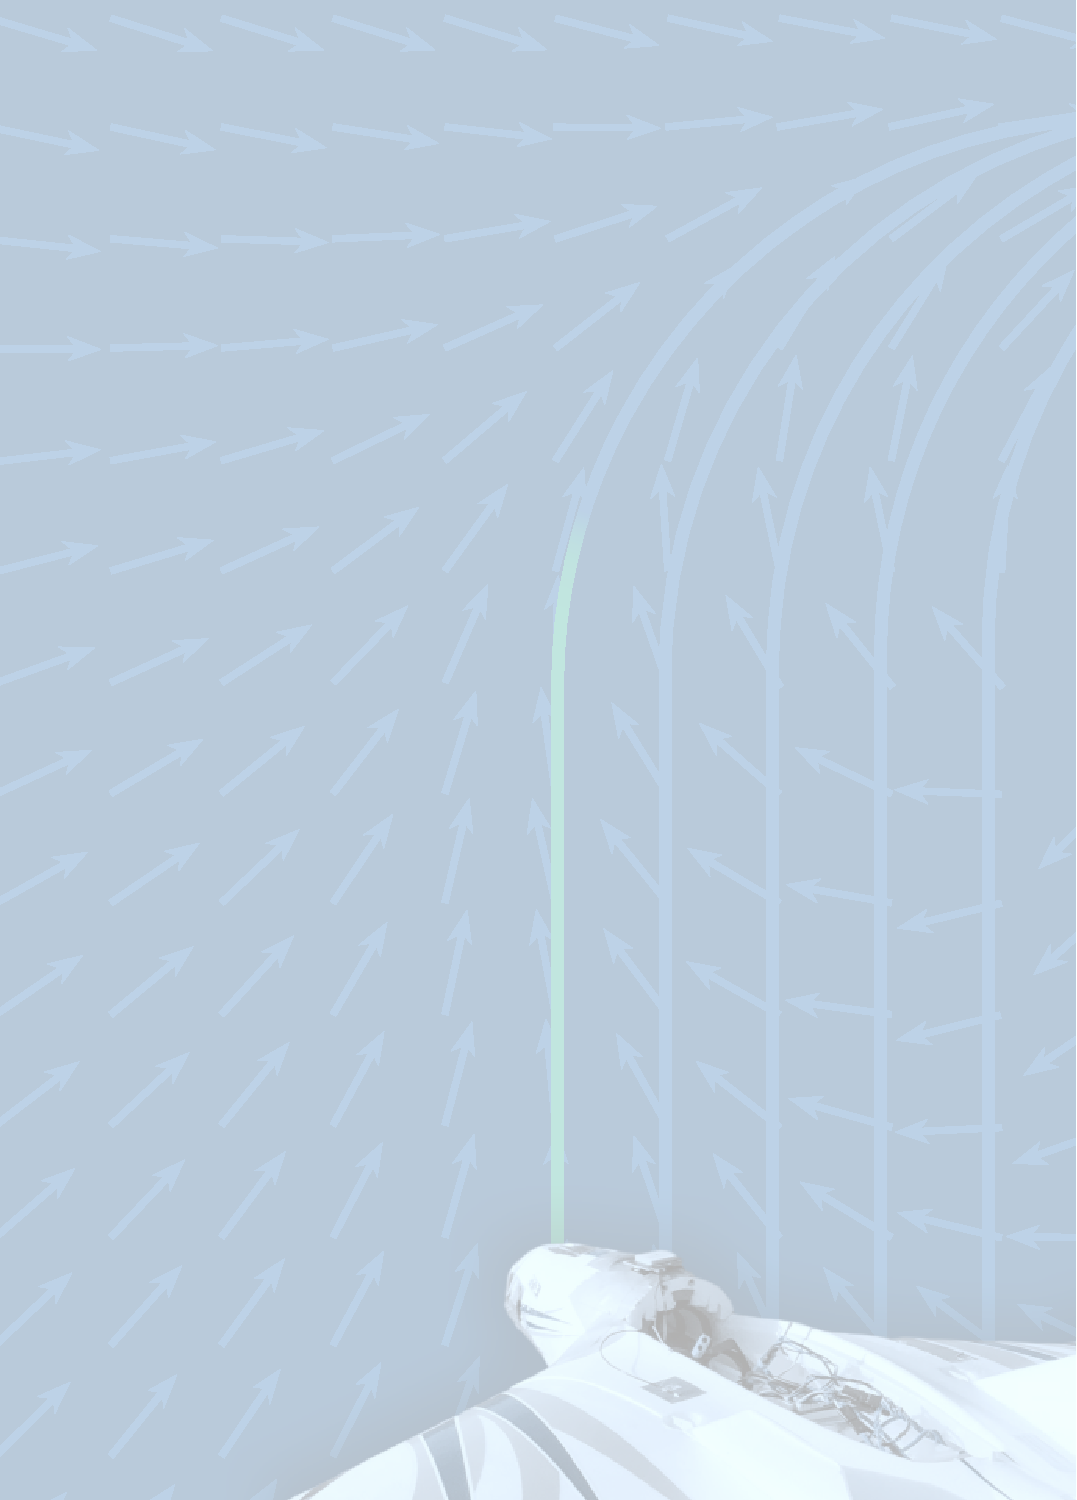
\includegraphics[width=\paperwidth,height=\paperheight]{figures/source/cover2.pdf}};
%{
%\centering
%	~
%}
%\cleardoublepage


\begin{titlepage}
	\centering
	{\large \publisher\par}
	~

	\vspace{36pt}
	{\Huge\fontfamily{phv}\selectfont\bfseries\booktitle\par}
	\vspace{24pt}

	\vspace{\stretch{1.25}}
	{\large A Dissertation submitted in partial satisfaction\par\vspace*{.8ex}
	of the requirements for the degree of\par\vspace*{.8ex}
	Doctor of Philosophy in Engineering Science}

	\vspace{12pt}
	{\large\itshape by\par}
	\vspace{6pt}
	{\Large\itshape \authorname\par}
	\vspace{24pt}

	{\begin{flushleft}{\itshape Approved by:}
		\begin{multicols}{2}
			{Ulrik Pagh Schultz, Advisor\\\vspace*{.8ex}
			~, Committee Member\\\vspace*{.8ex}
			~, Committee Member\\\vspace*{.8ex}
			~, Committee Chair\\
			}\par
			\columnbreak
			{~\\
			~\\
			~}\par
		\end{multicols}
		\vspace{6pt}
		\begin{multicols}{2}
		~\\\columnbreak {\itshape %Approved on: 
		                }
		\end{multicols}	
	\end{flushleft}}

	\vspace{\stretch{6}}
	{\large \editionyear{}}
\end{titlepage}



%%%%%%%%%%%%%%%%%%%%
%                  %
% Copyright page   %
%                  %
{\small\setlength{\parindent}{0em}\setlength{\parskip}{1em}
~

\vfill

\url{https://doi.org/10.21996/022y-wk34}

The typesetting is done using \LaTeX. Figures are generated with PGF/Ti\textit{k}Z. Fonts are EB Garamond, Helvetica, and Iwona for body, headers, and equations respectively.

Copyright \copyright{} 2021 by \authorname. Some rights reserved.

This work is subject to CC BY-NC-SA license, which means that you can copy, redistribute, remix, transform, and build upon the content for any non commercial purpose, as long as you give appropriate credit, provide a link to the license, and indicate if changes were made. If you remix, transform, or build upon the material, you must distribute your contributions under the same license as the original. License details: \url{https://creativecommons.org/licenses/by-nc-sa/4.0/}

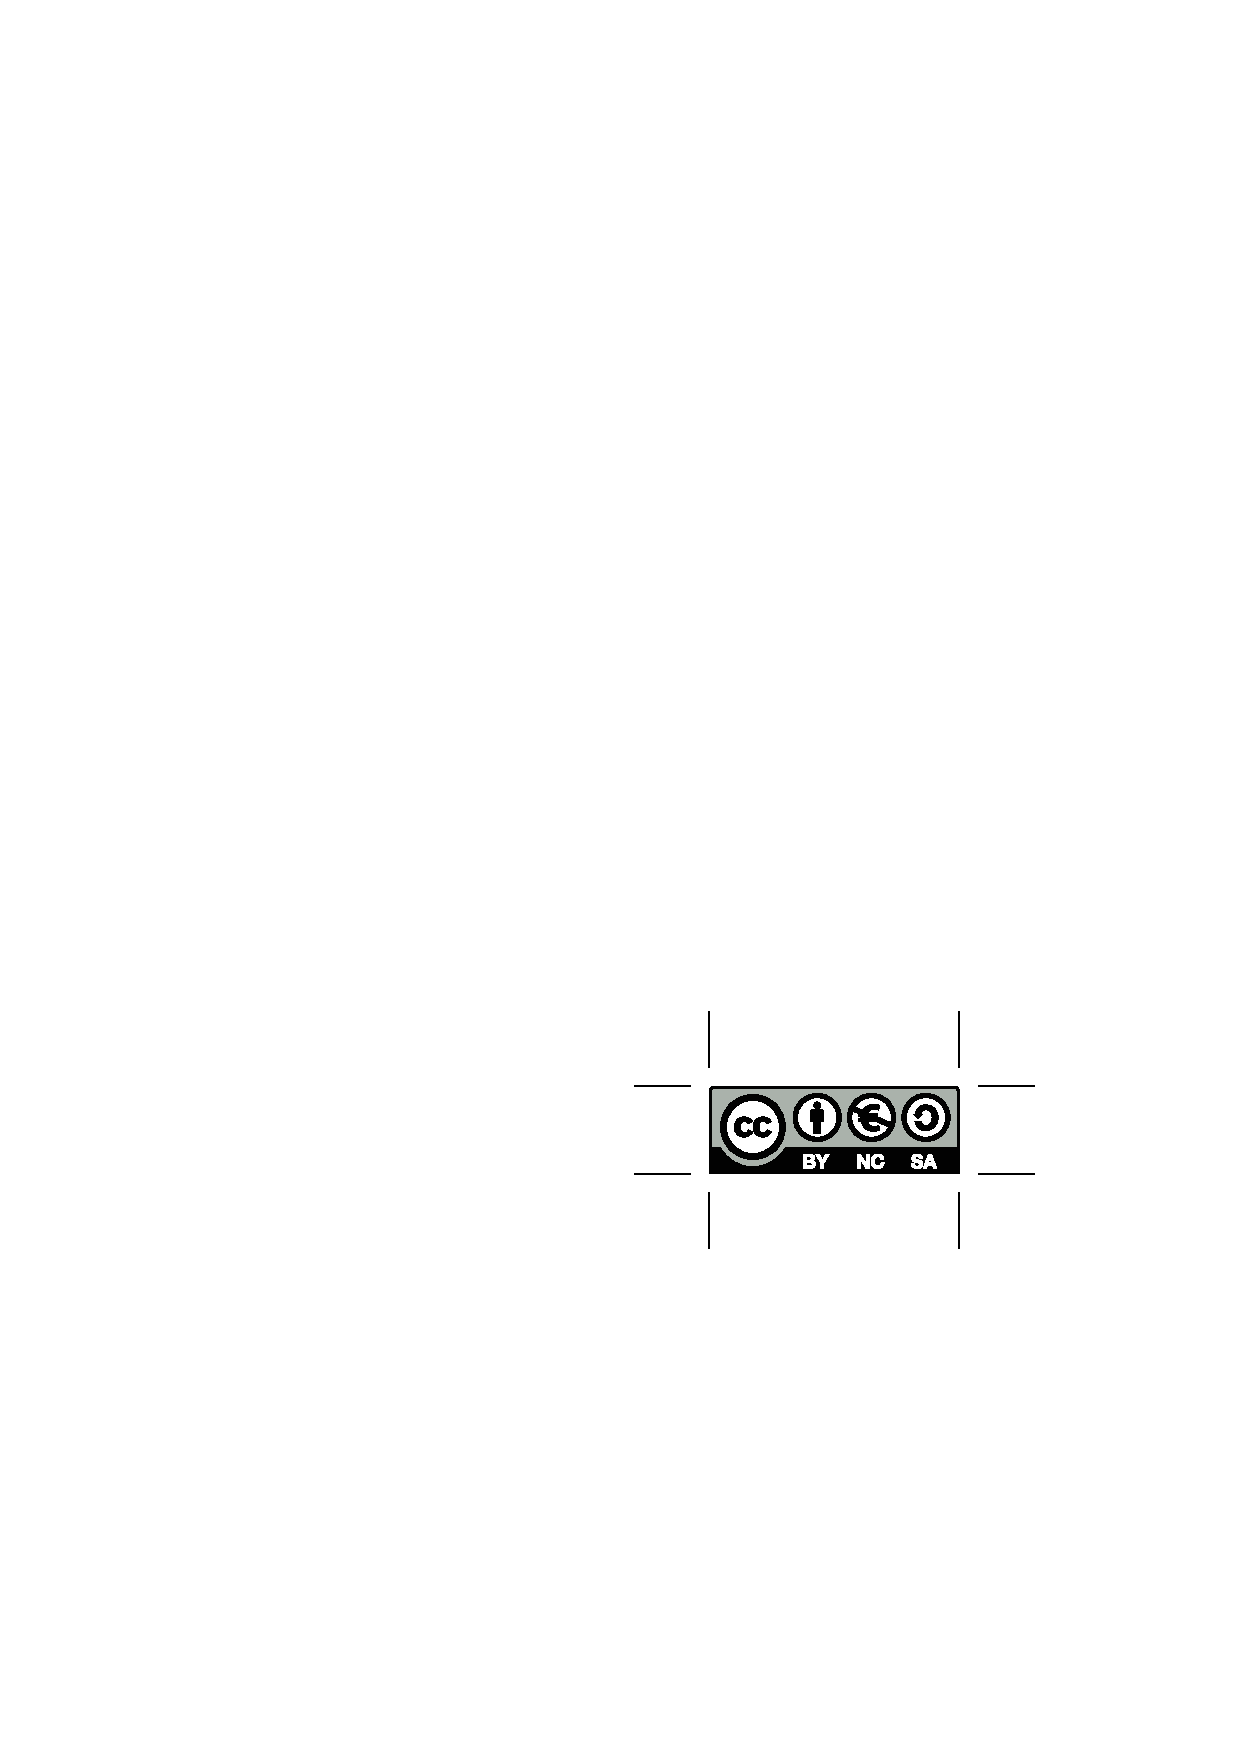
\includegraphics[width=.2\textwidth]{by-nc-sa}

First edition, \editionyear{}

%ISBN \isbn{} 

Published by \publisher{}, in \place{}
}\cleardoublepage

% dedication
\pagestyle{empty}\begin{center} 
    \thispagestyle{empty}
    \vspace*{\fill}\raggedleft\large
    To\dots
    
    \vspace*{\fill}
\end{center}\cleardoublepage
\pagestyle{fancy}

%%%%%%%%%%%%%%%%%%%%%%
%                    %
% Acknowledgements   %
%                    %
\chapter*{\color{red}Acknowledgements}

%\lettrine{A}{a}

\cleardoublepage   % tocpage on right-side

\thispagestyle{empty} 
\pagestyle{fancy}\tableofcontents\cleardoublepage\thispagestyle{empty} % toc
\renewcommand{\numberline}[1]{\hspace*{-1.5em}}
\pagestyle{fancy}\listoffigures\cleardoublepage\thispagestyle{empty} % list of figures
\pagestyle{fancy}\printunsrtglossary[type=notation,style=long]\cleardoublepage\thispagestyle{empty} % notation
\pagestyle{fancy}\printunsrtglossary[type=acronym,style=long]\cleardoublepage\thispagestyle{empty} % acronyms


%%%%%%%%%%%%%%%%
               %
% Mainmatter   %
               %
\mainmatter
\pagestyle{fancy}

%%%%%%%%%%%%%%%%%%
%                %
% Introduction   %
%                %
\chapter{Introduction}
\label{cp:intro}

%\begin{highlight}
%    \begin{st}
%        General structure with just some dummy text.
%    \end{st} 
%\end{highlight}

\lettrine{M}{obile robots} are a class of robots with the ability to move through the environment~\citep{corke2017robotics}. Most of these robots are power-demanding devices constrained by battery limitations. Whilst such limitations are a common challenge in many areas, they are critical in mobile robots' design and development, where they impact the level of autonomy~\citep{seewald2020mechanical}. This in turn is expected to increase in the foreseeable future~\citep{fisher2013verifying}.

To achieve the motion, mobile robots combine different components which sense and interact with the surrounding environment~\citep{mei2006deployment}. The analysis and interpretation of data originating from these components require energy-demanding heterogeneous mobile computing hardware. Planning energy-aware paths with a power-saving scheduler policy on such hardware is an underrepresented topic in the literature, even though the energy needed for the computations can almost equal the actuation in some instances of low-energy mobile robots~\citep{sudhakar2020balancing}. Due to the recent advancements in the computational capabilities of mobile hardware, such as the introduction of powerful portable GPUs~\citep{rizvi2017general}, the use of computations is expected to increase~\citep{abramov2012real,satria2016real,jaramillo2019visual}.

Aerial mobile robots, or more commonly Unmanned aerial vehicles (\Gls{acr:uav})s, are mobile robots with even more stringent battery limitations. Recharging the battery during normal operation is rarely an option, as it would require to land to replace or recharge the battery~\citep{zamanakos2020energy}. They are being increasingly used in applications such as monitoring, meteorology, robotics research, surveillance, search and rescue, and agriculture.


\section{A Brief History of Aerial Robotics}

After the Wright brothers worked so hard to put humans in the air in flying machines, a hundred years later some are working hard to take them out of flying machines~\citep{anderson2005introduction}.


\section{Motivation}

Many scenarios involving unmanned aerial vehicles (UAVs), such as precision agriculture, search and rescue, and surveillance, require high autonomy but have limited energy budgets. A typical example of these scenarios is a UAV following a path and performing some on-board computational tasks. For instance, the UAV might detect ground patterns and notify other ground-based actors with little human interaction. We refer to such computational tasks that can be dynamically replanned and adapted as \emph{computations}. We are interested in the energy optimization of the path and computations under uncertainty (atmospheric interferences) and refer to it as energy-aware dynamic planning. Such planning would find optimal tradeoffs between the path, computations, and energy requirements. Current generic planning solutions for outdoor UAVs do not plan the path and computations dynamically, nor are they energy-aware. They are often semi-autonomous: the path and computations are static and usually defined using planning software~\citep{daponte2019review} (for instance~\citep{papa} and~\citep{px4}). Such a state of practice has prompted us to propose an \emph{energy-aware dynamic planning algorithm} for UAVs. The algorithm combines and generalizes some of the past body of knowledge on mobile robot planning problems and addresses the increasing \emph{computational demands} and their relation to energy consumption, path, and autonomy for the UAV planning problem.

\section{Objective}


\section{Outline of the Approach}

Unlike most of the past planning algorithms literature, our algorithm plans the path and computations simultaneously. To model the path we use multiple mathematical functions. For instance, the path might contain multiple circles and lines. To model the computations we use \powprof{}, a profiling tool presented in previous work~\citep{seewald2019coarse}. To guide the UAV we use a vector field~\citep{de2017guidance} that converges to the path. The use of vector fields for guidance is widely discussed in the literature~\citep{lindemann2005smoothly,gonccalves2010vector,panagou2014motion,zhou2014vector,kapitanyuk2017guiding,de2017guidance}. 


To achieve the energy-aware dynamic planning, we further introduce and formally prove a periodic energy model that accounts for the uncertainty. We use Fourier analysis to derive the model, and state estimation to address the uncertainty. Periodicity is often present due to repetitive patterns in the plan~\citep{seewald2020mechanical}. Indeed, UAV scenarios often iterate over a set of tasks and paths (e.g., monitoring or search and rescue). Given that the plan is periodic, we expect the energy consumption to approximately evolve periodically. Some collected energy data from a UAV flying a survey scenario along its power spectrum motivates our choice.

% add these plots

In the spirit of reducing costs and resources, we showcase the algorithm using dynamic planning for a precision agriculture fixed-wing UAV. Precision agriculture is often put into practice~\citep{hajjaj2014review} with ground mobile robots used for harvesting~\citep{qingchun2012study,dong2011development, de2011design, aljanobi2010setup, li2008analysis, edan2000robotic}, and UAVs for preventing damage and ensuring better crop quality~\citep{puri2017agriculture, daponte2019review}. The plan is structured as follows. Path-wise, the UAV flies in circles and lines covering a polygon. Computation-wise, it detects hazards using a neural network and notifies grounded mobile robots employed for, e.g., harvesting. The algorithm alters the plan; it controls the processing rate and the radius of the circles (affecting the distance between the lines). 

We observe that not only the path but also the computations significantly impact the energy, with a potential extension of up to 13 minutes over an hour by switching from the highest to the lowest level of computations in presence of a standard battery.

\section{Applications}

\section{Problem Formulation}
\label{cp:intro:pb}

Let us adopt the following mathematical notation. Given an integer $a$, $[a]$ is the set $\{0,1,\dots,a\}$, $[a]^+$ the set $[a]/\{0\}$. Bold lower-case letters indicates vectors. $c_{i,j}$ the $j$-th parameter of the $i$-th parameters set $c_i$. $\underline{c}_{i,j},\overline{c}_{i,j}$ are the lower and upper bounds of the parameter $c_{i,j}$.

\begin{figure}[h]
  \center
  \begin{tikzpicture}[shorten >=.5pt,node distance=12.5ex,on grid,auto]
    \node[state,initial] (q_i) {$\Gamma_1$}; 
    \node        [right=of q_i] (q_dots0) {$\cdots$};
    \node[state] (q_0) [right=of q_dots0] {$\Gamma_i$};
    \node        (q_dots1) [right=of q_0] {$\cdots$};
    \node[state,accepting] (q_f) [right=of q_dots1] {$\Gamma_f$};
    \path[->]
    (q_i) edge node {$\mathbf{p}_{\Gamma_{1}}$} (q_dots0)
    (q_dots0) edge node{$\mathbf{p}_{\Gamma_{i-1}}$} (q_0)
    (q_0) edge node {$\mathbf{p}_{\Gamma_i}$} (q_dots1)
    (q_dots1) edge node {$\mathbf{p}_{\Gamma_{l}}$} (q_f)    
    (q_i) edge [loop above] node {$\mathbf{p}_{k_1}$} (q_i)
    (q_0) edge [loop above] node {$\mathbf{p}_{k_2}$} (q_0)
    (q_f) edge [loop above] node {$\mathbf{p}_{k_3}$} (q_f)
    ; %end path 
    \draw [decorate,decoration={brace,amplitude=10pt,mirror,raise=10pt},yshift=0pt]
    (q_i.south west) -- (q_f.south west) node [black,midway,yshift=-9ex]{$\Gamma$};
  \end{tikzpicture}
  \caption{The plan defined as a FSM}
  \label{fig:state-machine}
\end{figure}

Let us assume that the path at stage $i$ can be altered with $\rho$ path parameters
\begin{equation}
    c_i^\rho:=\{c_{i,1},c_{i,2},\dots,c_{i,\rho}\},
\end{equation}
and the computations with $\sigma$ computation parameters 
\begin{equation}
    c_i^\sigma:=\{c_{i,\rho+1},c_{i,\rho+2},\dots,c_{i,\rho+\sigma}\}.
\end{equation}

We then express the path as a continuous twice differentiable function $\varphi_i:\mathbb{R}^2\times\mathbb{R}^\rho\rightarrow\mathbb{R}$ of a point and the path parameters. The function returns a metric of the distance between the point and the nominal trajectory. We express the computations as the value of the computation parameters. We discuss the concrete meaning of the value of path parameters in \fref{cp:model}{Chapter}.

\begin{highlight}  
  \begin{defn}[Stage, plan, triggering, and final point]\label{def:mission}
    The $i$-th \emph{stage} $\Gamma_i$ at time instant $k$ of a plan $\Gamma$ is defined
    \begin{equation*}\begin{split}
      \Gamma_i:=\{\varphi_i(\mathbf{p}_k,c_i^\rho),c_i^\sigma\mid
      \,&\exists\,\,\mathbf{p}_k,\,\varphi_i(\mathbf{p}_k,c_i^\rho)\in\mathcal{C}_i,\,\\
        &\,\forall j\in[\sigma]^+,\,c_{i,\rho+j}\in\mathcal{S}_{i,j}\,\},
    \end{split}\end{equation*}
    where $\mathcal{C}_i:=[\underline{c}_i,\overline{c}_i]\subseteq\mathbb{R}$ is the path constraint set, and $\mathcal{S}_{i,j}:=[\underline{c}_{i,\rho+j},\overline{c}_{i,\rho+j}]\subseteq\mathbb{Z}_{\geq 0}$ the $j$-th computation constraint set. $\mathbf{p}_k$ is a point of a UAV flying at an altitude $h\in\mathbb{R}_{>0}$ w.r.t. some inertial navigation frame $\mathcal{O}_W$.
  
    The \emph{plan} is a finite state machine (FSM) $\Gamma$ where the state-transition function $s:\bigcup_i{\Gamma_i}\times\mathbb{R}^2\rightarrow\bigcup_i{\Gamma_i}$ maps a stage and a point to the next stage
    \begin{equation*}s(\Gamma_i,\mathbf{p}_k):=\begin{cases}
      \Gamma_{i+1} & \text{if }\mathbf{p}_k=\mathbf{p}_{\Gamma_i}\\
      \Gamma_i & \text{otherwise}
    \end{cases}.\end{equation*}
    The point $\mathbf{p}_{\Gamma_{i}}$ that allows the transition between $\Gamma_i$ and $\Gamma_{i+1}$ is called \emph{triggering point}. The last triggering point $\mathbf{p}_{\Gamma_{l}}$ relative to the last stage $\Gamma_l$ is called \emph{final point}.
  \end{defn}
\end{highlight}

\begin{figure}[t]
    \centering
    
\definecolor{c989898}{RGB}{152,152,152}
\definecolor{cDEDEDE}{RGB}{222,222,222}
\definecolor{cFFFFFF}{RGB}{255,255,255}
\definecolor{c2B2B2B}{RGB}{43,43,43}
\definecolor{c9B9B9B}{RGB}{155,155,155}


\def \globalscale {1.000000}
\begin{tikzpicture}[y=0.80pt, x=0.80pt, yscale=-1.1*\globalscale, xscale=1.1*\globalscale, inner sep=0pt, outer sep=0pt]
\path[draw=c989898,line join=round,line width=0.512pt] (37.9773,138.5660) -- (35.3357,138.5630);



  \path[fill=cDEDEDE,line join=round,even odd rule,line width=0.160pt] (59.2379,138.5360) -- (37.3300,138.5360) .. controls (37.3300,104.2680) and (65.1100,76.4881) .. (99.3784,76.4881) -- (99.3784,98.1778) .. controls (77.1987,98.3164) and (59.2589,116.3290) .. (59.2379,138.5360) -- cycle;



  \path[fill=cDEDEDE,line join=round,even odd rule,line width=0.160pt] (36.8146,208.2220) -- (59.2401,208.2220) -- (59.2407,138.0860) -- (36.8151,138.0860) -- (36.8146,208.2220) -- cycle;



  \path[fill=cDEDEDE,line join=round,even odd rule,line width=0.160pt] (75.5064,138.3220) -- (53.5984,138.3220) .. controls (53.5984,104.0540) and (81.3785,76.2741) .. (115.6470,76.2741) -- (115.6470,97.9639) .. controls (93.4671,98.1025) and (75.5273,116.1150) .. (75.5064,138.3220) -- cycle;



  \path[fill=cDEDEDE,line join=round,even odd rule,line width=0.160pt] (115.5600,97.9479) -- (115.5600,76.0399) .. controls (149.8280,76.0399) and (177.7080,103.8200) .. (177.7080,138.0880) -- (156.0190,138.0880) .. controls (155.8800,115.9090) and (137.7680,97.9688) .. (115.5600,97.9479) -- cycle;



  \path[fill=cDEDEDE,line join=round,even odd rule,line width=0.160pt] (53.0716,208.2330) -- (75.4972,208.2330) -- (75.4974,138.0950) -- (53.0718,138.0950) -- (53.0716,208.2330) -- cycle;



  \path[fill=cDEDEDE,line join=round,even odd rule,line width=0.160pt] (155.9570,208.2190) -- (178.3830,208.2190) -- (178.3990,137.9630) -- (155.9730,137.9630) -- (155.9570,208.2190) -- cycle;



  \path[draw=c989898,line join=round,line width=0.512pt] (99.5543,138.9930) ellipse (1.7511cm and 1.7511cm);



  \path[cm={{1.0,0.0,0.0,1.0,(190.0,175.0)}}] (0.0000,0.0000) node[above right] () {$\mathbf{p}_{k_4}$};



    \path[fill=cFFFFFF,line join=round,line width=0.160pt,rounded corners=0.0000cm] (65.5184,186.6300) rectangle (81.7257,202.8374);



    \path[cm={{1.0,0.0,0.0,1.0,(66.0,199.0)}}] (0.0000,0.0000) node[above right] () {$\varphi_1$};



  \path[draw=c2B2B2B,line join=round,line width=0.512pt] (115.6970,138.4880) ellipse (1.7511cm and 1.7511cm);



  \path[draw=c2B2B2B,line join=round,line width=0.512pt] (53.2806,50.4116) -- (53.2808,208.0220);



  \path[draw=c2B2B2B,line join=round,line width=0.512pt] (177.8300,50.4301) -- (177.8300,208.0410);



  \path[draw=c2B2B2B,line join=round,line width=0.512pt] (118.1030,140.8340) -- (113.8230,136.5520);



  \path[draw=c2B2B2B,line join=round,line width=0.512pt] (113.8260,140.8310) -- (118.1070,136.5500);



  \path[fill=black,line join=round,line width=0.256pt] (52.5078,197.6220) -- (52.5078,192.2880) -- (53.7878,192.2880) -- (53.7878,197.6220) -- (52.5078,197.6220) -- cycle(52.5078,186.9550) -- (52.5077,181.6220) -- (53.7877,181.6220) -- (53.7877,186.9550) -- (52.5078,186.9550) -- cycle(52.5077,176.2890) -- (52.5077,170.9550) -- (53.7877,170.9550) -- (53.7877,176.2890) -- (52.5077,176.2890) -- cycle(52.5077,165.6220) -- (52.5077,160.2890) -- (53.7877,160.2890) -- (53.7877,165.6220) -- (52.5077,165.6220) -- cycle(52.5076,154.9550) -- (52.5076,149.6220) -- (53.7876,149.6220) -- (53.7876,154.9550) -- (52.5076,154.9550) -- cycle(52.5076,144.2890) -- (52.5076,138.9550) -- (53.7876,138.9550) -- (53.7876,144.2890) -- (52.5076,144.2890) -- cycle(53.0267,133.5810) -- (53.1252,132.8330) -- (53.8254,128.9130) -- (53.9747,128.2740) -- (55.2289,128.5300) -- (55.0796,129.1680) -- (54.3905,133.0260) -- (54.2992,133.7200) -- (53.0267,133.5810) -- cycle(55.2719,123.0650) -- (56.4670,119.0750) -- (56.8957,117.9440) -- (58.1090,118.3510) -- (57.6804,119.4830) -- (56.5094,123.3920) -- (55.2719,123.0650) -- cycle(58.8505,112.9310) -- (61.1435,108.1160) -- (62.3221,108.6150) -- (60.0291,113.4300) -- (58.8505,112.9310) -- cycle(63.8781,103.4730) -- (64.7913,101.9480) -- (66.9793,99.0624) -- (68.0419,99.7761) -- (65.8539,102.6620) -- (65.0079,104.0740) -- (63.8781,103.4730) -- cycle(70.4287,94.9101) -- (74.1486,91.0881) -- (75.1213,91.9201) -- (71.4014,95.7421) -- (70.4287,94.9101) -- cycle(78.4053,87.7408) -- (80.3745,86.2019) -- (82.9136,84.7517) -- (83.6288,85.8132) -- (81.0897,87.2634) -- (79.2622,88.6916) -- (78.4053,87.7408) -- cycle(87.6306,82.0689) -- (92.6007,80.1345) -- (93.1529,81.2893) -- (88.1827,83.2237) -- (87.6306,82.0689) -- cycle(97.7391,78.4275) -- (102.9360,77.2307) -- (103.3130,78.4540) -- (98.1160,79.6508) -- (97.7391,78.4275) -- cycle(108.2830,76.3988) -- (113.5950,75.9193) -- (113.7960,77.1835) -- (108.4840,77.6630) -- (108.2830,76.3988) -- cycle(119.0310,75.9276) -- (124.3360,76.4738) -- (124.2840,77.7527) -- (118.9790,77.2066) -- (119.0310,75.9276) -- cycle(129.6590,77.4030) -- (134.8450,78.6494) -- (134.6300,79.9113) -- (129.4440,78.6648) -- (129.6590,77.4030) -- cycle(139.9380,80.4796) -- (144.0440,82.1042) -- (144.9200,82.6049) -- (144.3640,83.7578) -- (143.4890,83.2571) -- (139.5520,81.7000) -- (139.9380,80.4796) -- cycle(149.5490,85.2532) -- (150.9890,86.0768) -- (153.9650,88.3831) -- (153.2520,89.4460) -- (150.2750,87.1396) -- (148.9930,86.4062) -- (149.5490,85.2532) -- cycle(158.1060,91.8657) -- (161.8580,95.6554) -- (161.0080,96.6118) -- (157.2550,92.8221) -- (158.1060,91.8657) -- cycle(165.1950,99.9168) -- (166.1480,101.1420) -- (168.1780,104.4180) -- (167.1250,105.1460) -- (165.0960,101.8700) -- (164.2320,100.7590) -- (165.1950,99.9168) -- cycle(170.7940,109.1320) -- (172.2860,112.1330) -- (173.0420,114.0250) -- (171.8730,114.5450) -- (171.1170,112.6530) -- (169.6740,109.7510) -- (170.7940,109.1320) -- cycle(174.9250,119.0630) -- (175.9740,122.3380) -- (176.4510,124.2150) -- (175.2200,124.5650) -- (174.7430,122.6880) -- (173.7200,119.4930) -- (174.9250,119.0630) -- cycle(177.6310,129.4510) -- (177.8280,130.4450) -- (178.2610,133.3030) -- (178.4240,134.7830) -- (177.1550,134.9460) -- (176.9910,133.4660) -- (176.5670,130.6630) -- (176.3820,129.7310) -- (177.6310,129.4510) -- cycle(178.5140,140.1950) -- (178.5100,145.5280) -- (177.2300,145.5270) -- (177.2340,140.1940) -- (178.5140,140.1950) -- cycle(178.5060,150.8610) -- (178.5020,156.1950) -- (177.2220,156.1940) -- (177.2260,150.8600) -- (178.5060,150.8610) -- cycle(178.4970,161.5280) -- (178.4930,166.8610) -- (177.2130,166.8600) -- (177.2170,161.5270) -- (178.4970,161.5280) -- cycle(178.4890,172.1950) -- (178.4850,177.5280) -- (177.2050,177.5270) -- (177.2090,172.1940) -- (178.4890,172.1950) -- cycle(178.4810,182.8610) -- (178.4800,184.3970) -- (177.2000,184.3960) -- (177.2010,182.8600) -- (178.4810,182.8610) -- cycle(52.5078,208.2880) -- (52.5078,202.9550) -- (53.7878,202.9550) -- (53.7878,208.2880) -- (52.5078,208.2880) -- cycle;



    \path[fill=cFFFFFF,line join=round,line width=0.160pt,rounded corners=0.0000cm] (170.4340,62.4618) rectangle (186.6414,78.6691);



    \path[cm={{1.0,0.0,0.0,1.0,(170.0,75.0)}}] (0.0000,0.0000) node[above right] () {$\varphi_4$};



  \path[fill=cFFFFFF,line join=round,line width=0.160pt,rounded corners=0.0000cm] (151.1930,87.1333) rectangle (167.4004,103.3407);



  \path[cm={{1.0,0.0,0.0,1.0,(154.0,98.0)}}] (0.0000,0.0000) node[above right] () {$\varphi_5$};



  \path[cm={{1.0,0.0,0.0,1.0,(16.0,120.0)}}] (0.0000,0.0000) node[above right] () {$\mathbf{p}_{k_3}$};



  \path[draw=c989898,line join=round,line width=0.512pt] (101.6410,140.7130) -- (97.3588,136.4310);



  \path[draw=c989898,line join=round,line width=0.512pt] (97.3620,140.7090) -- (101.6430,136.4300);



  \path[draw=c989898,line join=round,line width=0.512pt] (37.4683,50.2362) -- (37.4674,207.8470);



  \path[draw=black,line join=round,line width=1.024pt] (37.3655,139.1460) .. controls (37.3655,108.3180) and (59.8482,82.7404) .. (89.3117,77.9160);



  \path[draw=black,line join=round,line width=1.024pt] (37.4074,138.8430) -- (37.4612,139.4260);



  \path[draw=black,line join=round,line width=1.024pt] (104.8160,14.6465) .. controls (114.1410,17.1626) and (116.3470,26.7356) .. (116.3470,26.7355) .. controls (116.3470,26.7355) and (134.0140,69.7724) .. (87.7439,78.3357);



  \path[draw=black,fill=cFFFFFF,line join=round,line width=0.512pt] (38.0214,129.9470) -- (48.4265,113.7660) -- (41.6299,114.7590) -- (36.4969,110.7700) -- (38.0214,129.9470) -- cycle;



  \path[draw=black,line join=round,line width=1.024pt] (37.3995,208.3130) -- (37.3999,138.8280);



    \path[fill=cFFFFFF,line join=round,line width=0.160pt,rounded corners=0.0000cm] (48.2360,62.4618) rectangle (64.4433,78.6691);



    \path[cm={{1.0,0.0,0.0,1.0,(46.0,75.0)}}] (0.0000,0.0000) node[above right] () {$\varphi_6$};



  \path[draw=black,line join=round,line width=0.512pt] (38.2486,129.1090) -- (41.5789,114.8440);



  \path[draw=black,fill=cFFFFFF,line join=round,line width=0.512pt] (75.8501,81.3976) -- (95.0620,82.3957) -- (90.0278,77.8124) -- (91.7396,70.5527) -- (75.8501,81.3976) -- cycle;



  \path[draw=black,line join=round,line width=0.512pt] (76.2742,81.2804) -- (89.9006,77.8114);



  \path[draw=black,line join=round,line width=1.024pt] (177.8490,208.2210) -- (177.8490,158.6520);



  \path[draw=black,fill=c9B9B9B,line join=round,line width=0.512pt] (177.8340,156.5720) -- (171.4330,174.7140) -- (177.8190,172.1830) -- (183.7320,174.8830) -- (177.8340,156.5720) -- cycle;



  \path[draw=black,line join=round,line width=0.512pt] (177.8060,157.4410) -- (177.8490,172.0900);



  \path[draw=black,fill=cFFFFFF,line join=round,line width=0.512pt] (122.5820,36.7240) -- (118.0690,18.0488) -- (113.9380,22.8537) -- (107.6780,24.6001) -- (122.5820,36.7240) -- cycle;



  \path[draw=black,line join=round,line width=0.512pt] (11.2790,8.9418) -- (11.2790,38.5413);



  \path[draw=black,line join=round,line width=0.512pt] (40.6757,38.3017) -- (11.0761,38.3017);



  \path[cm={{1.0,0.0,0.0,1.0,(1.0,52.0)}}] (0.0000,0.0000) node[above right] () {$\mathcal{O}_W$};



  \path[draw=black,line join=round,line width=0.512pt] (12.2122,38.1596) -- (114.5840,24.7774);



    \path[fill=cFFFFFF,line join=round,line width=0.160pt,rounded corners=0.0000cm] (49.3746,20.2690) rectangle (73.7139,36.4553);



    \path[cm={{1.0,0.0,0.0,1.0,(53.0,35.0)}}] (0.0000,0.0000) node[above right] () {$\mathbf{p}_{k_1}$};



  \path[draw=black,line join=round,line width=0.512pt] (113.9240,22.8546) -- (122.4610,36.6020);



  \path[fill=black,line join=round,line width=0.160pt] (38.7120,35.2069) -- (38.7201,41.3379) -- (44.3321,38.2655) -- (38.7120,35.2069) -- cycle;



  \path[fill=black,line join=round,line width=0.160pt] (8.2258,10.6325) -- (14.3568,10.6281) -- (11.2877,5.0143) -- (8.2258,10.6325) -- cycle;



  \path[fill=black,line join=round,line width=0.160pt] (109.5870,22.7566) -- (110.5860,28.8056) -- (115.6270,24.8662) -- (109.5870,22.7566) -- cycle;



    \path[fill=cFFFFFF,line join=round,line width=0.160pt,rounded corners=0.0000cm] (29.9808,62.4618) rectangle (46.1881,78.6691);



    \path[cm={{1.0,0.0,0.0,1.0,(27.0,75.0)}}] (0.0000,0.0000) node[above right] () {$\varphi_2$};



\path[draw=c2B2B2B,line join=round,line width=0.512pt] (179.6380,138.6350) -- (177.4990,138.6330);



\path[draw=c2B2B2B,line join=round,line width=0.512pt] (53.7370,138.6060) -- (51.0981,138.6060);



  \path[fill=cFFFFFF,line join=round,line width=0.160pt] (185.5880,202.9890) -- (173.1380,202.9890) -- (173.1040,215.0630) -- (185.5830,215.0320) -- (185.5880,202.9890) -- cycle;



  \path[cm={{1.0,0.0,0.0,1.0,(176.0,213.0)}}] (0.0000,0.0000) node[above right] () {$\overline{c}_4$};



  \path[fill=cFFFFFF,line join=round,line width=0.160pt] (160.5750,202.9910) -- (148.1260,202.9910) -- (148.0920,215.0660) -- (160.5710,215.0350) -- (160.5750,202.9910) -- cycle;



  \path[cm={{1.0,0.0,0.0,1.0,(151.0,213.0)}}] (0.0000,0.0000) node[above right] () {$\underline{c}_4$};




\path[cm={{1.0,0.0,0.0,1.0,(14.0,143.0)}}] (0.0000,0.0000) node[above right] () {$\mathbf{p}_{\Gamma_1}$};



\path[fill=cFFFFFF,line join=round,line width=0.160pt,rounded corners=0.0000cm] (62.9567,132.2440) rectangle (79.1640,148.4513);



\path[cm={{1.0,0.0,0.0,1.0,(66.0,144.0)}}] (0.0000,0.0000) node[above right] () {$\mathbf{p}_{\Gamma_5}$};



\path[cm={{1.0,0.0,0.0,1.0,(183.0,143.0)}}] (0.0000,0.0000) node[above right] () {$\mathbf{p}_{\Gamma_4}$};



\path[draw=black,line join=round,line width=0.512pt] (99.5120,138.7510) -- (99.5120,76.7023);



\path[fill=black,line join=round,line width=0.160pt] (97.1960,80.5069) -- (101.9120,80.5006) -- (99.5490,76.1842) -- (97.1960,80.5069) -- cycle;



  \path[fill=cFFFFFF,line join=round,line width=0.160pt] (108.2100,108.6570) -- (90.4810,108.6560) -- (90.4810,121.1060) -- (108.2100,121.1060) -- (108.2100,108.6570) -- cycle;



  \path[cm={{1.0,0.0,0.0,1.0,(93.0,120.0)}}] (0.0000,0.0000) node[above right] () {$c_{1,1}$};




\end{tikzpicture}


    \caption[Definition notation on a slice of the plan]{Definition notation shown on an slice of the plan.}
    \label{fig:traj1}
\end{figure}

The altitude $h$ from \fref{def:mission}{Definition} might change at different flying phases and under different atmospheric conditions

In \fref{fig:traj1}{Figure}, $\varphi_1,\dots,\varphi_6$ are paths. $\varphi_1$ and $\varphi_5$ are circles, while $\varphi_2$, $\varphi_4$, and $\varphi_6$ are lines. They are all relative to different stages $\Gamma_1,\Gamma_2,\dots$. The constraints set $\mathcal{C}_1,\mathcal{C}_2,\dots$ forms the area where the paths $\varphi_1,\varphi_2,\dots$ can be altered with the parameters $c_{i,1},\dots,c_{i,\rho}$ (gray area in the figure). This area is bounded by $\underline{c}_i,\overline{c}_i$, and can be different per each stage \fref{fig:traj1}{Figure}, the area relative to $\Gamma_4$ is bounded by $\underline{c}_4,\overline{c}_4$).

In \fref{fig:traj1}{Figure}, $\mathbf{p}_{\Gamma_1}$ allows the transition between $\Gamma_1$ and $\Gamma_2$, $\mathbf{p}_{\Gamma_4}$ between $\Gamma_4$ and $\Gamma_5$, and $\mathbf{p}_{\Gamma_5}$ between $\Gamma_5$ and $\Gamma_6$.

A slice of the plan in \fref{fig:state-machine}{Figure} shows the transition between the stages with the FSM. The triggering point $\mathbf{p}_{\Gamma_{i-1}}$ allows the transition to the stage $\Gamma_i$. The UAV remains in the stage with any generic point $\mathbf{p}_{k_2}$. It eventually enters the stage $\Gamma_{i+1}$ with the triggering point $\mathbf{p}_{\Gamma_i}$ and so on, until it reaches the final point. The stage $\Gamma_f$ is the accepting stage (it indicates that the UAV has completed the plan).

\begin{figure}[h]
  \center
  \begin{tikzpicture}[shorten >=1pt,node distance=27ex,on grid,auto] 
    \node        (q_dots0) {$\cdots$};
    \node[state] (q_0) [right=of q_dots0] {$\Gamma_i$};
    \node        (q_dots1) [right=of q_0] {$\cdots$};   
    \path[->]
    (q_dots0) edge node{$\mathbf{p}_{\Gamma_{i-1}}(c_1^\rho,\dots,c_{i-1}^\rho)$} (q_0)
    (q_0) edge node {$\mathbf{p}_{\Gamma_i}(c_1^\rho,\dots,c_{i}^\rho)$} (q_dots1)    
    (q_0) edge [loop above] node {$\mathbf{p}_{k}$} (q_0)
    ; %end path
  \end{tikzpicture}
\caption[Detail of a stage in the FSM]{Detail of the stage $\Gamma_i$ in the FSM}
\label{fig:state-machine2}
\end{figure}
    
Generally, one can express the triggering points in function of the $i$-th trajectory parameters $c_{i}^{\rho}$, or any previous trajectory parameters, propagating the information therein if necessary (see \fref{fig:state-machine2}{Figure}).
   

\subsection{Problem formulation}

In order to simplify the problem formulation, we consider some primitive paths. All the other paths are built from these paths with a shift $\mathbf{d}:=(x_d,y_d)$.

Given $n\in\mathbb{Z}_{>0}$ ($n<l,l/n\in\mathbb{Z}$) primitive paths $\varphi_1,\dots\varphi_n$, a generic starting point $\mathbf{p}$ and the current levels of the path parameters $c_1^\rho$, all the other paths $\varphi_{n+1},\dots,\varphi_l$ are built
\begin{equation}\label{eq:primitive}\begin{split}
  &\varphi_{(i-1)n+j}(\mathbf{p}+(i-1)\mathbf{d},c_1^\rho)-\\ &\,\,\,\varphi_{in+j}(\mathbf{p}+i\mathbf{d},c_1^\rho)=e_j,
\end{split}\end{equation}
$\forall i\in[l/n-1]^+,j\in[n]^+$, where $e_j\in\mathbb{R}$ is the $j$-th constant difference.

\begin{highlight}
\begin{defn}[Period]\label{def:period}
  The period $T\in\mathbb{R}_{> 0}$ is the time between $\varphi_{(i-1)n+j}$ and $\varphi_{in+j}$ in \frefeq{eq:primitive}.
\end{defn} 
\end{highlight}

The algorithm measures the time between the paths and assumes the initial period is one. The periods might be different for different $j$s due to atmospheric interferences.

One can define the plan using primitive paths or define all the stages explicitly and find $n$ searching the value which satisfies the \frefeq{eq:primitive}. If there is no such value, (e.g., when the plan is composed of only one stage), the period $T$ from \fref{def:period}{Definition} can be determined empirically from energy data.

\begin{highlight}
\begin{pb}[UAV planning problem]\label{pb}
  Consider an initial plan $\Gamma$ from \fref{def:mission}{Definition}. We are interested in the planning of the parameters $c_i,\,\forall i\in[l]^+$ and energy constraints and in the guidance of the UAV to the path resulting from such plan.
\end{pb}    
\end{highlight}

\section{Structure}



%
%%%%%%%%%%%%%%%%%%%%%%%%%
%                       %
% Problem Formulation   %
%                       %
%%%%%%%%%%%%%%%%%%%%%%%%%
%
% Brief abstract: formulates the two problem (coverage, (re)planning)
%
% Completion (1-10): 10
% Missing: -
% Proofreading: 11/10/21
%
\chapter{Problem Formulation}
\label{cp:pb}

\begin{chapquote}{\cite{arkin2001optimal}}
  ``While we will often speak of the [coverage] problem as `milling' with a `cutter', many of its important applications arise in various contexts outside of machining.''
\end{chapquote}

\vspace*{1em}

\lettrine{I}{n this chapter}, we discuss the planning and coverage problems that we are interested in solving. The coverage problem is the problem of finding the path that covers all the points in a given space~\citep{choset2001coverage,galceran2013survey}, for instance, the agricultural field in \fref{sec:motivation}{Section}. The coverage path with some user-defined computations forms the plan. The planning problem is then the problem of replanning the plan. It is replanned energy-wise in the eventuality of energy constraints dissatisfaction, and whenever the uncertainty affects the flight unexpectedly. To define both the problems, we need some basic constructs. In particular, we provide formal definitions in \fref{sec:definitions}{Sections}\fref{sec:defs-stages-triggs}{--\hspace*{-.8ex}} that include the computations, motion, computations energy, and motion energy. We then define the difference between computations and motion energy (\Gls{acr:mace}), which we encountered in \fref{sec:aerial-robo-types}{Section}, path, and other plan-specific constructs. In \fref{sec:2pbs}{Section}, we use all these to formulate the planning and coverage problems. We illustrate the problem with an example of the precision agriculture use case in \fref{sec:flight-plan}{Section}.

In \fref{cp:dyn}{Chapter}, we propose two algorithms. A first algorithm generates the coverage path, and another algorithm replans the plan in time, solving the coverage and planning problems. The replanning is energy-aware: the algorithm outputs the best trajectory of the path and computations alteration for an aerial robot with varying battery and atmospheric conditions. 

The chapter connects to the remainder of this work as follows. Here we formalize the plan, the planning and coverage problems, and some other basic constructs. We use the plan characteristics to derive an energy model in \fref{cp:model}{Chapter}. We solve the planning problem with modern optimal control techniques and the coverage problem using a coverage path planning (\Gls{acr:cpp})\findex{coverage path planning} algorithm in \fref{cp:dyn}{Chapter}. We guide the aerial robot with a vector field, using the plan's building blocks from this chapter. We show the solutions to the problems experimentally in \fref{cp:res}{Chapter}. We discuss past approaches to solve the problems in \fref{cp:soa}{Chapter}.% and the concrete implementation in \fref{app:imp}{Appendix}.


%%%%%%%%%%%%%%%%%%%%%%%%%%%%%%%%%%%%%%%%%%%%%%%%
\section{Definitions of computations and motion}
\label{sec:definitions}

First, we define computations and motion along with their energy and M\&CE. Our planning-scheduling depends on these basic concepts.

\begin{defn}[Computations/motion]
  \label{def:comps}
  \emph{Computations}\findex{computations} are energy-demanding computational tasks. The aerial robot runs the computations on heterogeneous computing hardware that interfaces microcontrollers.
  \emph{Motion}\findex{motion} is the act of the aerial robot moving in the surrounding environment. For this purpose, the aerial robot runs some primitives on microcontrollers that interface actuators, motors, and other components.
\end{defn}

Autonomous capabilities are often achieved by interconnecting heterogeneous computing hardware and microcontrollers. For the computations, we assume that the heterogeneous computing hardware runs a schedule parametrized by some parameters. For instance, for the detection computation from the precision agriculture scenario in \fref{sec:objective}{Section}, a parameter is the frames per second (\Gls{acr:fps})\findex{frames per second} rate. Alike for the computations, for the motion, we assume that the robot travels some paths parametrized by some other parameters. For instance, for the coverage, a parameter changes the coverage quality.

\begin{defn}[Computations/motion and overall energy]
  \label{def:comp-mot-energy}
  Given a path parametrized by $\rho$ parameters $c_i^\rho:=\{c_{i,1},c_{i,2},\dots,c_{i,\rho}\}$, the \emph{motion energy}\findex{motion energy} is the energy spent by the aerial robot while moving on the path.
  Given a schedule parametrized by parameters $c_i^\sigma:=\{c_{i,\rho+1},c_{i,\rho+2},\dots,c_{i,\rho+\sigma}\}$, the \emph{computations energy}\findex{computations energy} is the energy spent by heterogeneous computing hardware executing the schedule.
  The \emph{overall energy}\findex{overall energy} is the sum of motion energy and computations energy.
\end{defn}

Physically, motion energy is the energy spent by all the systems powering the aerial robot, excluding the heterogeneous computing hardware. We use watts for instantaneous or average measures of computations, motion, and overall energies, whereas joules for measures over a given time interval. We show in \fref{sec:defs-stages-triggs}{Section} what we mean by the parametrization of paths and computations with some parameters.

\Gls{acr:mace}\findex{difference of motion and computations energy} that we introduced in \fref{sec:aerial-robo-types}{Section} is the difference between average motion and computations energy. It is measured in watts, and it gives a measure of which of the two energy components is predominant. For \Gls{acr:mace} greater than zero, the motion energy dominates over the computations. The dynamic planning approach plans first an energy-efficient path. If we return briefly to \fref{fig:robots-vs-power}{Figure}, it is the case for rotary-wing aerial robots \sref{lab:matrice} and \sref{lab:agras}. On the contrary, for \Gls{acr:mace} lower than zero, the computations energy dominates. The dynamic planning approach plans first a power-saving schedule. It is the case for the lighter-than-air aerial robot \sref{lab:skye} in \fref{fig:robots-vs-power}{Figure}. For \Gls{acr:mace} close to zero, both energy components are important energy-wise. The dynamic planning approach plans both an energy-efficient path and a power-saving schedule to a similar extent. This M\&CE is characteristic of fixed-wing aerial robots, such as \sref{lab:cumulus}\fref{lab:opterra}{--\hspace*{-.8ex}} in \fref{fig:robots-vs-power}{Figure}.


%%%%%%%%%%%%%%%%%%%%%%%%%%%%%%%%%%%%%%
\section{Definition of path functions}
\label{sec:path-functions}

To model the path, we use multiple mathematical functions $\varphi_1,\varphi_2,\dots$ that we call path functions. These functions express the path in 2D space at an altitude $h\in\mathbb{R}$ for an inertial navigation frame $\mathcal{O}_W$. We discuss a generalization of the path functions in 3D space and how it affects the guidance in \fref{cp:conc}{Chapter}. 

\begin{defn}[Path functions]
  \label{def:paths}
  $\varphi_i:\mathbb{R}^2\rightarrow\mathbb{R},\,\forall i\in\{1,2,\dots\}$ are \emph{path functions}\findex{path functions} used to model the path. They are a function of a generic time-dependent point $\mathbf{p}(t):=(x_{\mathbf{p}(t)},y_{\mathbf{p}(t)})$ of the aerial robot flying in the 2D space and are continuous and twice differentiable. 
\end{defn}\findex{continuity}\findex{twice differentiability}

\begin{figure}[t!]
  \centering
  
\definecolor{cECECEC}{RGB}{236,236,236}
\definecolor{c989898}{RGB}{152,152,152}
\small

\def \globalscale {1.000000}
\begin{tikzpicture}[y=0.80pt, x=0.80pt, yscale=-.9*\globalscale, xscale=.9*\globalscale, inner sep=0pt, outer sep=0pt]
\path[fill=cECECEC,line join=round,line width=0.160pt] (338.3020,263.8010) -- (381.1050,-0.0001) -- (102.8640,12.1601) -- (58.1440,275.9610) -- (338.3020,263.8010) -- cycle;



\path[draw=c989898,line join=round,line width=0.512pt] (147.6250,213.3720) -- (173.5250,186.3120) -- (132.2780,180.7850);



\path[fill=c989898,line join=round,line width=0.256pt] (163.3290,190.5470) -- (158.3650,192.4980) -- (158.1310,191.9020) -- (163.0950,189.9520) -- (163.3290,190.5470) -- cycle(153.4020,194.4490) -- (148.4380,196.4000) -- (148.2040,195.8040) -- (153.1680,193.8530) -- (153.4020,194.4490) -- cycle(143.4740,198.3510) -- (138.5110,200.3020) -- (138.2760,199.7060) -- (143.2400,197.7550) -- (143.4740,198.3510) -- cycle(133.5470,202.2530) -- (128.5830,204.2040) -- (128.3490,203.6080) -- (133.3130,201.6570) -- (133.5470,202.2530) -- cycle(123.6200,206.1550) -- (118.6560,208.1060) -- (118.4220,207.5100) -- (123.3850,205.5590) -- (123.6200,206.1550) -- cycle(113.6920,210.0560) -- (108.7280,212.0070) -- (108.4940,211.4120) -- (113.4580,209.4610) -- (113.6920,210.0560) -- cycle(103.7650,213.9580) -- (100.0090,215.4350) -- (99.7748,214.8390) -- (103.5310,213.3630) -- (103.7650,213.9580) -- cycle(173.2570,186.6450) -- (168.2930,188.5960) -- (168.0590,188.0010) -- (173.0220,186.0500) -- (173.2570,186.6450) -- cycle;



\path[draw=c989898,line join=round,line width=0.512pt] (55.1846,208.3180) -- (99.4269,215.2590);



\path[draw=black,line join=round,line width=0.512pt] (68.2145,216.7950) -- (99.1080,215.5400);



\path[draw=c989898,line join=round,line width=0.512pt] (99.5793,215.0880) -- (196.7320,112.9950);



\path[draw=foo,line join=round,line width=0.512pt] (139.9040,221.4650) -- (147.6230,213.4870);



\path[draw=black,line join=round,line width=0.512pt] (99.6097,215.3190) -- (377.1250,258.8550);



\path[fill=foo,line join=round,line width=0.256pt] (163.7520,67.1159) -- (158.7880,69.0661) -- (158.5540,68.4704) -- (163.5180,66.5202) -- (163.7520,67.1159) -- cycle(153.8240,71.0164) -- (148.8600,72.9667) -- (148.6260,72.3709) -- (153.5900,70.4207) -- (153.8240,71.0164) -- cycle(143.8960,74.9168) -- (138.9320,76.8670) -- (138.6980,76.2713) -- (143.6620,74.3211) -- (143.8960,74.9168) -- cycle(133.9680,78.8173) -- (129.0040,80.7676) -- (128.7700,80.1719) -- (133.7340,78.2216) -- (133.9680,78.8173) -- cycle(124.0400,82.7178) -- (119.0760,84.6679) -- (118.8420,84.0722) -- (123.8060,82.1220) -- (124.0400,82.7178) -- cycle(114.1120,86.6182) -- (109.1480,88.5685) -- (108.9140,87.9728) -- (113.8780,86.0225) -- (114.1120,86.6182) -- cycle(104.1840,90.5187) -- (99.9651,92.1761) -- (99.7311,91.5804) -- (103.9500,89.9230) -- (104.1840,90.5187) -- cycle(173.6800,63.2155) -- (168.7160,65.1657) -- (168.4820,64.5700) -- (173.4460,62.6198) -- (173.6800,63.2155) -- cycle;



\path[draw=black,line join=round,line width=0.512pt] (99.6290,215.7460) -- (99.6701,45.2765);



\path[fill=black,line join=round,line width=0.160pt] (97.4234,50.0749) -- (99.6963,48.0699) -- (101.7800,50.0657) -- (99.5939,44.2973) -- (97.4234,50.0749) -- cycle;



\path[fill=black,line join=round,line width=0.160pt] (372.7840,255.6340) -- (374.2970,258.2610) -- (371.9260,259.9050) -- (378.0140,258.9110) -- (372.7840,255.6340) -- cycle;



\path[draw=c989898,fill=c989898,line join=round,line width=0.160pt] (191.9960,115.1180) -- (195.0250,115.0410) -- (195.3410,117.9090) -- (197.3700,112.0830) -- (191.9960,115.1180) -- cycle;



\path[draw=black,line join=round,line width=0.512pt] (99.6614,215.4240) -- (348.2110,205.3130);



\path[fill=black,line join=round,line width=0.256pt] (365.8960,204.3560) -- (371.2240,204.1220) -- (371.2520,204.7610) -- (365.9240,204.9950) -- (365.8960,204.3560) -- cycle(376.5520,203.8870) -- (381.8800,203.6530) -- (381.9080,204.2920) -- (376.5800,204.5270) -- (376.5520,203.8870) -- cycle(387.2080,203.4190) -- (391.6130,203.2250) -- (391.6410,203.8640) -- (387.2370,204.0580) -- (387.2080,203.4190) -- cycle(355.2390,204.8250) -- (360.5670,204.5900) -- (360.5960,205.2300) -- (355.2670,205.4640) -- (355.2390,204.8250) -- cycle;



\path[fill=black,line join=round,line width=0.256pt] (51.6916,217.8380) -- (46.3616,218.0290) -- (46.3388,217.3890) -- (51.6687,217.1990) -- (51.6916,217.8380) -- cycle(41.0317,218.2190) -- (35.7017,218.4090) -- (35.6789,217.7700) -- (41.0088,217.5790) -- (41.0317,218.2190) -- cycle(30.3718,218.6000) -- (25.0419,218.7900) -- (25.0190,218.1500) -- (30.3490,217.9600) -- (30.3718,218.6000) -- cycle(62.3514,217.4570) -- (57.0215,217.6480) -- (56.9986,217.0080) -- (62.3286,216.8180) -- (62.3514,217.4570) -- cycle;



\path[draw=black,line join=round,line width=0.512pt] (138.1150,223.3150) -- (140.0590,221.3710);



\path[draw=c989898,line join=round,line width=0.512pt] (129.6630,180.5070) -- (132.3930,180.8300);



\path[draw=c989898,line join=round,line width=0.512pt] (173.5260,186.3500) -- (173.5730,63.0377);



\path[draw=black,line join=round,line width=0.512pt] (96.7492,91.8181) -- (99.4988,91.8249);



\path[cm={{1.0,0.0,0.0,1.0,(376.0,276.0)}}] (0.0000,0.0000) node[above right] () {$x$};



\path[cm={{1.0,0.0,0.0,1.0,(198.0,102.0)}}] (0.0000,0.0000) node[above right] () {$y$};



\path[cm={{1.0,0.0,0.0,1.0,(85.0,46.0)}}] (0.0000,0.0000) node[above right] () {$z$};



\path[draw=black,line join=round,line width=0.512pt] (83.3760,232.1090) -- (99.6032,215.0620);



\path[fill=c989898,line join=round,line width=0.512pt] (173.2360,184.7230) .. controls (174.0900,184.7230) and (174.7820,185.4150) .. (174.7820,186.2700) .. controls (174.7820,187.1240) and (174.0900,187.8160) .. (173.2360,187.8160) .. controls (172.3810,187.8160) and (171.6890,187.1240) .. (171.6890,186.2700) .. controls (171.6890,185.4150) and (172.3810,184.7230) .. (173.2360,184.7230) -- cycle;



\path[cm={{1.0,0.0,0.0,1.0,(161.0,289.0)}}] (0.0000,0.0000) node[above right] () {$\varphi(x,y):=2y-x$};



\path[cm={{1.0,0.0,0.0,1.0,(353.0,224.0)}}] (0.0000,0.0000) node[above right] () {$2y-x=h$};



\path[cm={{1.0,0.0,0.0,1.0,(131.0,238.0)}}] (0.0000,0.0000) node[above right] () {$x_\mathbf{p}$};



\path[cm={{1.0,0.0,0.0,1.0,(113.0,180.9)}}] (0.0000,0.0000) node[above right] () {$y_\mathbf{p}$};



\path[cm={{1.0,0.0,0.0,1.0,(41.0,98.0)}}] (0.0000,0.0000) node[above right] () {$\varphi(\mathbf{p})=d$};



\path[draw=c989898,fill=c989898,line join=round,line width=0.160pt] (175.7670,179.7880) -- (173.4940,181.7930) -- (171.4110,179.7970) -- (173.5970,185.5660) -- (175.7670,179.7880) -- cycle;



\path[draw=c989898,fill=c989898,line join=round,line width=0.160pt] (171.2840,70.1412) -- (173.5570,68.1363) -- (175.6400,70.1321) -- (173.4540,64.3637) -- (171.2840,70.1412) -- cycle;



\path[fill=foo,line join=round,line width=0.512pt] (173.4160,61.7418) .. controls (174.2700,61.7418) and (174.9630,62.4342) .. (174.9630,63.2885) .. controls (174.9630,64.1427) and (174.2700,64.8351) .. (173.4160,64.8351) .. controls (172.5620,64.8351) and (171.8700,64.1427) .. (171.8700,63.2885) .. controls (171.8700,62.4342) and (172.5620,61.7418) .. (173.4160,61.7418) -- cycle;



  \path[fill=cECECEC,line join=round,line width=0.160pt] (182.5940,102.1690) -- (164.2430,102.1690) -- (164.1940,119.9680) -- (182.5870,119.9220) -- (182.5940,102.1690) -- cycle;



  \path[cm={{1.0,0.0,0.0,1.0,(170.0,116.0)}}] (0.0000,0.0000) node[above right] () {$d$};



\path[cm={{1.0,0.0,0.0,1.0,(187.0,186.0)}}] (0.0000,0.0000) node[above right] () {$(x_\mathbf{p},y_\mathbf{p},h)$};


\path[draw=c989898,line join=round,line width=0.512pt] (99.6154,255.8180) -- (99.6251,215.7290);


\end{tikzpicture}


  \caption[Concept of a line as a path function]{The path is a mathematical function $\varphi(\mathbf{p}(t))=h$ that represents a line at an altitude $h$. A generic point $\mathbf{p}$ in 2D space intersects the plane formed by $\varphi$ at a value $d$ of the $z$-axis.}
  \label{fig:line-pf}
\end{figure}

\begin{figure}[t!]
  \centering
  
\definecolor{c989898}{RGB}{152,152,152}
\definecolor{cFFFFFF}{RGB}{255,255,255}
\small

\def \globalscale {1.000000}
\begin{tikzpicture}[y=0.80pt, x=0.80pt, yscale=-\globalscale, xscale=\globalscale, inner sep=0pt, outer sep=0pt]

\path[cm={{1.0,0.0,0.0,1.0,(0,0)}}] (10.0000,23.0000) node[below right] () {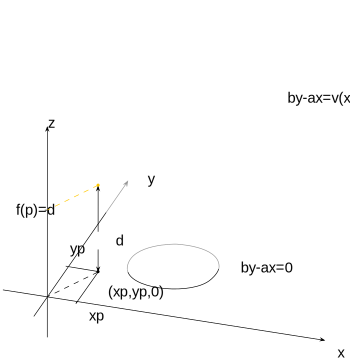
\includegraphics{figures/source/plot11}};


\path[draw=black,line join=round,line width=0.512pt] (2.8949,290.3560) -- (47.1372,297.2970);



\path[draw=black,line join=round,line width=0.512pt] (47.3200,297.3570) -- (324.8360,340.8930);



\path[draw=black,line join=round,line width=0.512pt] (47.3393,297.7850) -- (47.3804,127.3150);



\path[draw=black,line join=round,line width=0.512pt] (47.3257,337.8570) -- (47.3354,297.7680);



\path[draw=black,line join=round,line width=0.512pt] (47.2678,297.6320) -- (106.3620,212.7130);



\path[draw=c989898,line join=round,line width=0.512pt] (106.3620,212.7130) -- (127.7670,181.9530);



\path[fill=black,line join=round,line width=0.160pt] (45.1337,132.1130) -- (47.4066,130.1080) -- (49.4901,132.1040) -- (47.3042,126.3360) -- (45.1337,132.1130) -- cycle;



\path[fill=black,line join=round,line width=0.160pt] (320.4950,337.6720) -- (322.0070,340.2990) -- (319.6360,341.9440) -- (325.7240,340.9500) -- (320.4950,337.6720) -- cycle;



\path[cm={{1.0,0.0,0.0,1.0,(323.0,358.0)}}] (0.0000,0.0000) node[above right] () {$x$};



\path[cm={{1.0,0.0,0.0,1.0,(33.0,128.0)}}] (0.0000,0.0000) node[above right] () {$z$};



\path[cm={{1.0,0.0,0.0,1.0,(133.0,184.0)}}] (0.0000,0.0000) node[above right] () {$y$};



\path[draw=c989898,fill=c989898,line join=round,line width=0.160pt] (123.4090,184.7720) -- (126.3910,184.2350) -- (127.1390,187.0210) -- (128.2590,180.9550) -- (123.4090,184.7720) -- cycle;



\path[draw=black,line join=round,line width=0.512pt] (33.8410,316.9190) -- (47.2875,297.6020);



\path[draw=c989898,line join=round,line width=0.512pt] (219.3400,268.1300) .. controls (219.4020,267.7210) and (219.4350,267.3120) .. (219.4350,266.9020) .. controls (219.4350,246.0390) and (175.9680,244.5180) .. (175.9680,244.5180) .. controls (175.9680,244.5180) and (131.4840,243.8660) .. (127.5750,266.9020) .. controls (127.3910,267.9820) and (127.3660,269.0270) .. (127.4870,270.0360);



\path[draw=c989898,line join=round,line width=0.512pt] (127.4870,270.0360) .. controls (127.5930,270.9220) and (127.8120,271.7810) .. (128.1350,272.6120);



\path[draw=black,line join=round,line width=0.512pt] (128.1350,272.6120) .. controls (135.2830,291.0080) and (193.4860,295.5780) .. (210.9770,280.0880) .. controls (210.9770,280.0880) and (217.3970,275.0510) .. (219.0510,269.4220);



\path[draw=c989898,line join=round,line width=0.512pt] (219.0510,269.4220) .. controls (219.1760,268.9940) and (219.2750,268.5630) .. (219.3400,268.1300);



\path[draw=black,line join=round,line width=0.512pt] (76.1806,303.7580) -- (98.6304,272.0580) -- (68.5307,267.0880);



\path[fill=black,line join=round,line width=0.256pt] (88.4047,277.5740) -- (83.6131,279.9160) -- (83.3321,279.3410) -- (88.1237,276.9990) -- (88.4047,277.5740) -- cycle(78.8215,282.2580) -- (74.0299,284.6000) -- (73.7488,284.0250) -- (78.5405,281.6830) -- (78.8215,282.2580) -- cycle(69.2382,286.9420) -- (64.4466,289.2840) -- (64.1656,288.7090) -- (68.9572,286.3670) -- (69.2382,286.9420) -- cycle(59.6550,291.6260) -- (54.8634,293.9680) -- (54.5823,293.3930) -- (59.3740,291.0510) -- (59.6550,291.6260) -- cycle(50.0718,296.3100) -- (47.4163,297.6080) -- (47.1352,297.0330) -- (49.7907,295.7350) -- (50.0718,296.3100) -- cycle(97.9880,272.8900) -- (93.1964,275.2320) -- (92.9153,274.6570) -- (97.7069,272.3150) -- (97.9880,272.8900) -- cycle;



\path[draw=black,line join=round,line width=0.512pt] (75.8932,304.1100) -- (77.5142,301.8890);



\path[draw=black,line join=round,line width=0.512pt] (65.8149,266.5770) -- (68.5286,267.0200);



\path[fill=black,line join=round,line width=0.160pt] (98.1795,270.5460) .. controls (99.0337,270.5460) and (99.7262,271.2390) .. (99.7262,272.0930) .. controls (99.7262,272.9470) and (99.0337,273.6400) .. (98.1795,273.6400) .. controls (97.3253,273.6400) and (96.6329,272.9470) .. (96.6329,272.0930) .. controls (96.6329,271.2390) and (97.3253,270.5460) .. (98.1795,270.5460) -- cycle;



\path[draw=black,line join=round,line width=0.512pt] (98.2198,273.2710) -- (98.2658,184.9590);



\path[fill=black,line join=round,line width=0.160pt] (100.4610,266.7090) -- (98.1879,268.7140) -- (96.1044,266.7190) -- (98.2904,272.4870) -- (100.4610,266.7090) -- cycle;



\path[fill=black,line join=round,line width=0.160pt] (95.9772,191.7620) -- (98.2501,189.7570) -- (100.3340,191.7530) -- (98.1477,185.9850) -- (95.9772,191.7620) -- cycle;



\path[fill=foo,line join=round,line width=0.160pt] (98.2177,183.9090) .. controls (99.0719,183.9090) and (99.7643,184.6020) .. (99.7643,185.4560) .. controls (99.7643,186.3100) and (99.0719,187.0020) .. (98.2177,187.0020) .. controls (97.3635,187.0020) and (96.6710,186.3100) .. (96.6710,185.4560) .. controls (96.6710,184.6020) and (97.3635,183.9090) .. (98.2177,183.9090) -- cycle;



  \path[fill=cFFFFFF,line join=round,line width=0.160pt] (106.2870,232.0900) -- (96.9368,232.0900) -- (84.8873,249.8890) -- (112.2810,249.8430) -- (106.2870,232.0900) -- cycle;



  \path[cm={{1.0,0.0,0.0,1.0,(93.0,246.0)}}] (0.0000,0.0000) node[above right] () {$d_2$};



\path[draw=black,line join=round,line width=0.512pt] (44.8080,210.4840) -- (47.5576,210.4910);



\path[cm={{1.0,0.0,0.0,1.0,(-16.0,215.0)}}] (0.0000,0.0000) node[above right] () {$\varphi(\mathbf{p})=d_2$};



\path[fill=foo,line join=round,line width=0.256pt] (88.6970,190.5360) -- (83.9057,192.8790) -- (83.6246,192.3040) -- (88.4160,189.9610) -- (88.6970,190.5360) -- cycle(79.1143,195.2210) -- (74.3229,197.5640) -- (74.0419,196.9890) -- (78.8332,194.6460) -- (79.1143,195.2210) -- cycle(69.5316,199.9060) -- (64.7402,202.2490) -- (64.4591,201.6740) -- (69.2505,199.3310) -- (69.5316,199.9060) -- cycle(59.9489,204.5910) -- (55.1575,206.9340) -- (54.8764,206.3590) -- (59.6678,204.0160) -- (59.9489,204.5910) -- cycle(50.3661,209.2760) -- (47.4761,210.6890) -- (47.1950,210.1140) -- (50.0850,208.7010) -- (50.3661,209.2760) -- cycle(98.2798,185.8510) -- (93.4884,188.1940) -- (93.2073,187.6190) -- (97.9987,185.2760) -- (98.2798,185.8510) -- cycle;



\path[cm={{1.0,0.0,0.0,1.0,(93.0,298.0)}}] (0.0000,0.0000) node[above right] () {$(x_{\mathbf{p}},y_{\mathbf{p}},h)$};



\path[cm={{1.0,0.0,0.0,1.0,(74.0,321.0)}}] (0.0000,0.0000) node[above right] () {$x_{\mathbf{p}}$};



\path[cm={{1.0,0.0,0.0,1.0,(55.0,254.0)}}] (0.0000,0.0000) node[above right] () {$y_{\mathbf{p}}$};



\path[cm={{1.0,0.0,0.0,1.0,(200.0,300.0)}}] (0.0000,0.0000) node[above right] () {$(x-3)^2+(y-3)^2-2=h$};



\path[cm={{1.0,0.0,0.0,1.0,(70.0,20.0)}}] (0.0000,0.0000) node[above right] () {$\varphi(x,y):=(x-3)^2+(y-3)^2-2$};




\end{tikzpicture}


  \caption[Concept of a circle as a path function]{The path function now represents a circle at an altitude $h$. $\mathbf{p}$ intersects the cone formed by $\varphi$ at a value $d_2$ of the $z$-axis.}
  \label{fig:circle-pf}
\end{figure}

We use this notion to guide the aerial robot using vector field\findex{vector field} in \fref{algo:grad-desc}{Algorithms}\fref{algo:track}{--\hspace*{-.8ex}} in \fref{cp:dyn}{Chapter}. For instance, one can define a line as a path function with
\begin{equation}\label{eq:basic-path}
  \varphi(x,y):=ax+by+c,
\end{equation}
where $a,b,c\in\mathbb{R}$ are given constants. The generic point $\mathbf{p}(t)$ intersects $\varphi(x,y)$ on a specific value $d$ of the $z$-axis $(\mathbf{p}(t),d)$. We illustrate the concept in \fref{fig:line-pf}{Figure} for $c$ zero and $a,b$ minus one and two and $h$ zero for simplicity. The point intersects the plane\findex{plane} formed by the path function\findex{line}
\begin{equation}\label{eq:pathf-line}
  \varphi(x,y):=2y-x,%-h, there is no minus h here (facepalm)
\end{equation}
at $d=\varphi(\mathbf{p})$. The path that the aerial robot follows is then $\varphi(x,y)=h$. $\varphi(\mathbf{p})-h$ is the distance on the $z$-axis.

Likewise with the line, one can define a circle as a path function with\findex{circle}
\begin{equation}\label{eq:pathf-circle}
  \varphi(x,y):=(x-x_c)^2+(y-y_c)^2-r^2,
\end{equation}
where $x_c,y_c$ are given coordinates of the center and $r\in\mathbb{R}_{>0}$ the radius. We illustrate the circle path function in \fref{fig:circle-pf}{Figure} for $x_c,y_c$ both three, $\sqrt{r}$ two, and $h$ zero for simplicity. 

In this work, we use lines and circles as path functions. We connect these functions using some specific points--the triggering points. However, one can define any mathematical function, with the only requirement being continuity and twice differentiability. We use the first derivative for the vector field, the second derivative to derive the control action. We explain the concept further in \fref{cp:dyn}{Chapter}.


%%%%%%%%%%%%%%%%%%%%%%%%%%%%%%%%%%%%%%%%%%%%%%%%%%%%%
\section{Definitions of stages and triggering points}
\label{sec:defs-stages-triggs}

The plan has several stages $i=\{1,2,\dots\}$, and we assume that at each stage $i$, the aerial robot runs a schedule and travels a path function $\varphi_i$ using a parameters set $c_i$.
Parameters are variable values that we use for replanning the path and computations since they influence the computations/motion energy in \fref{def:comp-mot-energy}{Definition}. The path parameters are real-valued variable values ($\mathbb{R}$), the computations parameters are integer-valued variable values ($\mathbb{Z}$). We use the notation  $c_{i,j}$ to denote the $j$th parameter of the $i$th parameters set
\begin{equation}
  c_i=\{c_{i,1},c_{i,2},\dots,c_{i,j},\dots\}.
\end{equation}

Parameters are bounded. $\underline{c}_{i,j}$ is the lower bound of the parameter $c_{i,j}$. $\overline{c}_{i,j}$ is the upper bound
\begin{equation}
  \underline{c}_{i,j}\leq c_{i,j}\leq\overline{c}_{i,j}.
\end{equation}

We assume there are $\rho$ \emph{path}-specific \emph{parameters}\findex{path parameters} and $\sigma$ \emph{computations}-specific \emph{parameters}\findex{computations parameters} for every stage. It means that the path at stage $i$ can be replanned with $\rho$ path parameters
$c_i^\rho:=\{c_{i,1},c_{i,2},\dots,c_{i,\rho}\}$,
whereas the computations (i.e., the energy-demanding computational task executed on heterogeneous computing hardware in \fref{def:comps}{Definition}) with $\sigma$ computation parameters 
$c_i^\sigma:=\{c_{i,\rho+1},c_{i,\rho+2},\dots,c_{i,\rho+\sigma}\}$.

Returning to \fref{sec:definitions}{Section}, by parametrization of the path with parameters, we mean that we enhance $\varphi_i$ with the path parameters $c_i^\rho$. $\varphi_i:\mathbb{R}^2\times\mathbb{R}^\rho\rightarrow\mathbb{R}$ is thus a (continuous twice differentiable) function of a point and the path parameters. We use the parameters to alter the path and change the energy consumption. Similarly, by parametrization of the schedule with parameters, we mean that we express the computations as the value of the computations parameters. These are also employed for energy alteration (by, e.g., decreasing the granularity of a given computation we lower instantaneous energy consumption). We discuss the alteration of the energy with path parameters and computation parameters further in \fref{sec:nom-cont}{Sections}\fref{sec:merging}{--\hspace*{-.8ex}}.

Since at every stage the aerial robot travels a path and executes a schedule both parametrized by the parameters, we define the stage as a set that contains the path and path and computations parameters.

\begin{defn}[Stage]
  \label{def:stage}
  For a generic point $\mathbf{p}(t)$, the $i$th \emph{stage}\findex{stage} $\Gamma_i$ at time instant $t$ of a plan $\Gamma$ is
  \begin{equation*}\begin{split}
    \Gamma_i:=\{\varphi_i(\mathbf{p}(t),c_i^\rho),c_i^\sigma\mid
    \,&\forall j\,\in\,[\rho]_{>0},\,c_{i,j}\,\,\,\,\,\,\,\in\mathcal{C}_{i,j},\,\\
      &\,\forall k\in[\sigma]_{>0},\,c_{i,\rho+k}\in\mathcal{S}_{i,k}\,\},
  \end{split}\end{equation*}
  where $\mathcal{C}_{i,j}:=[\underline{c}_{i,j},\overline{c}_{i,j}]\subseteq\mathbb{R}$ is the $j$th path parameter constraint set, and $\mathcal{S}_{i,k}:=[\underline{c}_{i,\rho+k},\overline{c}_{i,\rho+k}]\subseteq\mathbb{Z}_{\geq 0}$ the $k$th computation parameter constraint set.\findex{constraint set}
\end{defn}

We clarify in the next section why the stage contains the generic point of the aerial robot flying in 2D space.

For simplicity, we merge the computations and path constraint sets in a single constraint set. $i$th stage constraint set is then
\begin{equation}\label{eq:constraint-set}
  \mathcal{U}_i(c_{i,j}):=\begin{cases}
  \mathcal{C}_{i,j} & \text{for } c_{i,j} \text{ with } j\leq\rho\\
  \mathcal{S}_{i,j-\rho} & \text{for } c_{i,j} \text{ with } \rho<j\leq\sigma
\end{cases},\end{equation}
the stage can be thus simplified $\Gamma_i:=\{\varphi_i(\mathbf{p}(t),c_i^\rho),c_i^\sigma\mid \,\forall j\,\in\,[\rho+\sigma]_{>0},\,c_{i,j}\in\mathcal{U}_i(c_{i,j})\}$.


To move from a given stage $\Gamma_i$ to the next stage $\Gamma_{i+1}$, we define some specific points $\mathbf{p}_{\Gamma_i}$. As soon as the aerial robot reaches the proximity of these points, it switches to the next stage
\begin{equation}\label{eq:trig-vareps}
  \norm{\mathbf{p}(t)-\mathbf{p}_{\Gamma_i}}<\varepsilon,
\end{equation}
where $\varepsilon\in\mathbb{R}$ is a given constant value expressing the radius of an imaginary circle over the point $\mathbf{p}_{\Gamma_i}$.

\begin{defn}[Triggering and final point]\findex{triggering point}\findex{final point}\findex{final stage}
  \label{def:trigs}
  The point $\mathbf{p}_{\Gamma_{i}}$ that allows the transition between stages is called the \emph{triggering point}. The last triggering point $\mathbf{p}_{\Gamma_{l}}$ relative to the last stage $\Gamma_l$ is called the \emph{final point}.
\end{defn}


%%%%%%%%%%%%%%%%%%%%%%%%%%%%%%%%
\section{Definition of the plan}
\label{sec:plan}

Our motion energy model in \fref{sec:mot-ener-model}{Section} uses the concept of the aerial robot flying a set of paths and computations autonomously. Such an autonomous flight plan often presumes a certain degree of periodicity, which one can observe in the precision agriculture use case in \fref{sec:objective}{Section}. An exhaustive way to cover the agricultural field in \fref{fig:plot2}{Figure}, i.e., to visit all the points in the space, is to define a basic pattern. The aerial robot flies over the field once and iterates the basic pattern until it covers the desired area. In literature, we often talk about motion, with the most common being, e.g., boustrophedon motion~\citep{choset2005principles,choset2001coverage,cabreira2019survey,galceran2013survey}. It means that we can define the plan just as a set of stages, triggering points, a final point, and finally a shift that tells how these constructs (except the final point) shifts in space each period. To simplify the planning problem to this latter case of plans with a pattern iterated over time, we consider some primitive paths.

\begin{defn}[Primitive paths]
  \label{def:primitive}
  Given $n\in\mathbb{Z}_{>0}$, the paths $\varphi_1,\dots\varphi_n$ are called \emph{primitive paths}\findex{primitive paths} if all the remaining paths in the plan are built from these paths with a \emph{shift}\findex{shift} $\mathbf{d}:=(x_{\mathbf{d}},y_{\mathbf{d}})$. 
\end{defn}

Let us assume the number of stages in the plan is known and is $l\in\mathbb{Z}$. If the plan is built from the primitive paths, it means that $n$ in \fref{def:primitive}{Definition} respects the inequation
\begin{equation}
  n<l,\,l/n\in\mathbb{Z}.
\end{equation}
%This means that $n$ is a multiplier of $l$, whereas $l/n$ is the multiplicand. 
One can then write the remaining paths from the $n$ primitive paths as $\varphi_{n+1},$ $\varphi_{n+2},\dots,\varphi_{n+n},\dots,\varphi_l$, or more generally $\varphi_{(i-1)n+1},$ $\varphi_{(i-1)n+2},\dots,\varphi_{(i-1)n+n},\,\forall i\in[l/n-1]_{>0}$. It can also be written formally
\begin{equation}\label{eq:primitive}\begin{split}
  &\varphi_{(i-1)n+j}(\mathbf{p}+(i-1)\mathbf{d},c_1^\rho)-\varphi_{in+j}(\mathbf{p}+i\mathbf{d},c_1^\rho)=e_j,
\end{split}\end{equation}
for a given shift $\mathbf{d}$, initial point $\mathbf{p}$, and initial value of path parameters $c_1^\rho$. \frefeq{eq:primitive} holds $\forall i\in[l/n-1]_{>0},j\in[n]_{>0}$. $e_j\in\mathbb{R}$ is the $j$th constant difference.

Generally, if the plan is built from the primitive paths, it is not required to know a priori the number of stages $l$. The paths can be iterated up until the final point $\mathbf{p}_{\Gamma_l}$. We use the concept of primitive paths for the energy modeling in \fref{cp:model}{Chapter}, where we show from collected energy data that plans built from primitive paths often have a periodic energy evolution. Alternatively to the primitive paths, one can define the plan as a mere linear succession of stages along with the triggering and final points. In the latter case, the energy can be periodic, aperiodic, or semi-periodic. Aperiodicity affects the modeling, and thus future energy predictions. We discuss the concrete meaning of periodicity, aperiodicity, and semi-periodicity in the context of energy modeling in \fref{sec:non-perio}{Section}.

Formally, we define the plan as a finite state machine using the constructs of path functions in \fref{def:paths}{Definition} of stages and triggering points in \fref{def:stage}{Definitions}\fref{def:trigs}{--\hspace*{-.8ex}}.

\begin{defn}[Plan]
  \label{def:plan}
  For a generic point $\mathbf{p}(t)$, the \emph{plan} is a finite state machine\findex{finite state machine} (\Gls{acr:fsm}) $\Gamma$, where the state-transition function $s:\bigcup_i{\Gamma_i}\times\mathbb{R}^2\rightarrow\bigcup_i{\Gamma_i}$ maps a stage and a point to the next stage
  \begin{equation*}s(\Gamma_i,\mathbf{p}(t)):=\begin{cases}
    \Gamma_{i+j} & \exists j\in\mathbb{Z},\text{ if }\norm{\mathbf{p}(t)-\mathbf{p}_{\Gamma_i}}<\varepsilon\\
    \Gamma_i & \text{otherwise}
  \end{cases}.\end{equation*}
\end{defn}

The value $\varepsilon$ in \fref{def:plan}{Definition} is the same $\varepsilon$ in \frefeq{eq:trig-vareps}. We illustrate the definition of the plan, stage, triggering, and final points in \fref{fig:state-machine}{Figures}\fref{fig:state-machine-loop}{--\hspace*{-.8ex}}.

\begin{figure}[h!]
  \center
  \begin{tikzpicture}[shorten >=.5pt,node distance=12.5ex,on grid,auto,initial text=\footnotesize\fontfamily{phv}\selectfont{start}]
    \node[state,initial] (q_i) {$\Gamma_1$}; 
    \node        [right=of q_i] (q_dots0) {$\cdots$};
    \node[state] (q_0) [right=of q_dots0] {$\Gamma_i$};
    \node        (q_dots1) [right=of q_0] {$\cdots$};
    \node[state,accepting] (q_f) [right=of q_dots1] {$\Gamma_f$};
    \path[->]
    (q_i) edge node {$\mathbf{p}_{\Gamma_{1}}$} (q_dots0)
    (q_dots0) edge node{$\mathbf{p}_{\Gamma_{i-1}}$} (q_0)
    (q_0) edge node {$\mathbf{p}_{\Gamma_i}$} (q_dots1)
    (q_dots1) edge node {$\mathbf{p}_{\Gamma_{l}}$} (q_f)    
    (q_i) edge [loop above] node {$\mathbf{p}(t_1)$} (q_i)
    (q_0) edge [loop above] node {$\mathbf{p}(t_2)$} (q_0)
    (q_f) edge [loop above] node {$\mathbf{p}(t_3)$} (q_f)
    ; %end path 
    \draw [decorate,decoration={brace,amplitude=10pt,mirror,raise=10pt},yshift=0pt]
    (q_i.south west) -- (q_f.south west) node [black,midway,yshift=-9ex]{$\Gamma$};
  \end{tikzpicture}
  \caption[Definition of a plan]{Definition of a plan $\Gamma$ as an FSM. Each state is a stage $\Gamma_i$, the transition happens in the proximity of specific points called triggering points $\mathbf{p}_{\Gamma_i}$. The accepting stage $\Gamma_f$ indicates the termination of the plan.}
  \label{fig:state-machine}
\end{figure}
In \fref{fig:state-machine}{Figure}, we illustrate a plan with a linear succession of stages. The triggering point $\mathbf{p}_{\Gamma_{i-1}}$ allows the transition to the stage $\Gamma_i$. The robot remains in the stage with any generic point $\mathbf{p}(t_2)$, where $t_1<t_2<t_3$ are three different time instants. It eventually enters the stage $\Gamma_{i+1}$ with the triggering point $\mathbf{p}_{\Gamma_i}$ and so on, until it reaches the final point. $\Gamma_f$ is the accepting stage (it indicates that the robot has completed the plan).
\begin{figure}[h!]
  \center
  \begin{tikzpicture}[shorten >=1pt,node distance=27ex,on grid,auto]
    \node        (q_dots0) {$\cdots$};
    \node[state] (q_0) [right=of q_dots0] {$\Gamma_i$};
    \node        (q_dots1) [right=of q_0] {$\cdots$};   
    \path[->]
    (q_dots0) edge node{$\mathbf{p}_{\Gamma_{i-1}}(c_1^\rho,\dots,c_{i-1}^\rho)$} (q_0)
    (q_0) edge node {$\mathbf{p}_{\Gamma_i}(c_1^\rho,\dots,c_{i}^\rho)$} (q_dots1)    
    (q_0) edge [loop above] node {$\mathbf{p}(t_2)$} (q_0)
    ; %end path
  \end{tikzpicture}
  \caption[Detail of a stage in the FSM]{Detail of the stage $\Gamma_i$ in the FSM. The triggering points used to transition between states are expressed in the function of the last and/or previous path parameters.}
  \label{fig:state-machine2}
\end{figure}
In \fref{fig:state-machine2}{Figure}, we illustrate that generally, one can express the basic constructs--such as path functions and triggering points--in the function of the $i$th path parameters $c_{i}^{\rho}$, or any previous path parameters, propagating the information therein if necessary. We further expand on this notion in the example in \fref{sec:flight-plan}{Section}, where we propagate a path parameter to all the following triggering points and path functions.

\begin{figure}[h!]
  \center
  \begin{tikzpicture}[shorten >=.5pt,node distance=12.5ex,on grid,auto,initial text=\footnotesize\fontfamily{phv}\selectfont{start}]
    \node[state,initial] (q_i) {$\Gamma_1$}; 
    \node[state] (q_2) [right=of q_i] {$\Gamma_2$}; 
    \node        [right=of q_2] (q_dots0) {$\cdots$};
    \node[state] (q_0) [right=of q_dots0] {$\Gamma_n$};
    \node[state,accepting] (q_f) [right=of q_0] {$\Gamma_f$};
    \path[->]
    (q_i) edge node {$\mathbf{p}_{\Gamma_{1}}$} (q_2)
    (q_2) edge node {$\mathbf{p}_{\Gamma_{2}}$} (q_dots0)
    (q_dots0) edge node{$\mathbf{p}_{\Gamma_{n-1}}$} (q_0)
    (q_0) edge [bend right=65] node [above] {$\mathbf{p}_{\Gamma_n}$} (q_i)
    (q_i) edge [bend left=-65] node [above] {$\mathbf{p}_{\Gamma_l}$} (q_f)
    (q_2) edge [bend left=-45] node [above] {$\mathbf{p}_{\Gamma_l}$} (q_f)
    (q_0) edge node {$\mathbf{p}_{\Gamma_{l}}$} (q_f)    
    (q_i) edge [loop above] node {$\mathbf{p}(t_1)$} (q_i)
    (q_2) edge [loop above] node {$\mathbf{p}(t_2)$} (q_2)
    (q_0) edge [loop above] node {$\mathbf{p}(t_3)$} (q_0)
    (q_f) edge [loop above] node {$\mathbf{p}(t_4)$} (q_f)
    ; %end path 
    \draw [decorate,decoration={brace,amplitude=10pt,mirror,raise=60pt},yshift=0pt]
    (q_i.south west) -- (q_f.south west) node [black,midway,yshift=-22ex]{$\Gamma$};
  \end{tikzpicture}
  \caption[Definition of a plan with a loop]{Definition of a plan $\Gamma$ with periodic patterns. Stages $\Gamma_1,\Gamma_2,\dots,\Gamma_n$ containing primitive paths $\varphi_1,\varphi_2,\dots,\varphi_n$ are iterated with a shift $\mathbf{d}$.}
  \label{fig:state-machine-loop}
\end{figure}
In \fref{fig:state-machine-loop}{Figure}, we illustrate a plan composed of $n$ stages $\Gamma_1,\Gamma_2,\dots,\Gamma_n$ (containing primitive paths $\varphi_1,\varphi_2,\dots,\varphi_n$) that are reiterated with the shift $\mathbf{d}$. $t_3<t_4$ is another time instant. We will see in \fref{cp:dyn}{Chapter} that the algorithm that solves the coverage problem outputs primitive paths, and the corresponding plan to be replanned is equivalent to \fref{fig:state-machine-loop}{Figure}. 

A concept that we use in the remainder of this work, and particularly in energy modeling in \fref{cp:model}{Chapter}, is the period--the time required to fly the primitive paths $\varphi_1,\varphi_2,\dots,\varphi_n$ (or generally $\varphi_{(i-1)n+1},$ $\varphi_{(i-1)n+2},\dots,\varphi_{(i-1)n+n}$). 

\begin{defn}[Period]
  \label{def:period}\findex{period}
  For a given stage $\Gamma_i$ and $j\in\mathbb{Z}_{>0}$, the \emph{period}\findex{period} $T\in\mathbb{R}_{> 0}$ is the flight time measured in seconds between $\varphi_{(i-1)n+j}$ and $\varphi_{in+j}$.
\end{defn} 
  
We assume the initial period is one and measure the period required to fly the paths physically or in simulation. The periods might be different for different $j$s due to atmospheric interferences or replanning. For the path functions, the coverage algorithm defines the plan using primitive paths $\varphi_1,\varphi_2,\dots,\varphi_n$, but can alternatively define all the stages explicitly and find $n$ searching the value which satisfies the \frefeq{eq:primitive}. If there is no such value (e.g., when the plan is composed of only one stage or the plan is aperiodic), the period $T$ from \fref{def:period}{Definition} can be determined empirically from energy data.


%%%%%%%%%%%%%%%%%%%%%%%%%%%
\section{Problem Statement}
\label{sec:2pbs}

We split the overall strategy for energy-aware planning-scheduling into two sub-problems. The planning problem is the problem of replanning a plan, whereas the coverage problem is the problem of defining the coverage plan for a given space.  

\subsection{Planning problem}
\label{sec:plan-pb}

More precisely, the planning problem is then the problem of finding the optimal configurations of the parameters within some criteria. In our approach, we focus on energy criteria, such as the battery constraints. In particular, in the solution to the planning problem in \fref{sec:algo}{Section}, we use a cost function (i.e., the function to maximize) that incorporates the energy model in \fref{sec:mot-ener-model}{Section}. Solving the planning problem by finding the optimal configurations within different criteria, such as shortest time, highest security, path tracking with the shortest detour, or others, is equally possible. In the context of the TeamPlay project that funded a considerable part of this work, we aim to find, for instance, the tradeoffs between time, energy, and security criteria for a variety of use cases. We discuss the eventuality of solving the planning problem with different costs in \fref{cp:conc}{Chapter}. We now use the concepts in the previous sections and provide a formal definition of the planning problem that we are interested in solving in the remainder of this work.

\begin{pb}[Planning problem]
  \label{pb}\findex{planning problem}
  Consider an initial plan $\Gamma$ in \fref{def:stage}{Definition}. It is either composed of $l$ stages or $n$ stages and a shift $\mathbf{d}$. The \emph{planning problem} is the problem of finding the optimal configuration of \emph{path} and \emph{computations parameters} $c_i\,\forall i\in[l]_{>0}$ or $\forall i\in\{1,2,\dots\}$ under energy constraints and uncertainty at each time step $t$.
\end{pb}    

In the definition, there is a fixed or variable number of stages, in the sense that all the stages are reiterated using the primitive paths in \fref{def:primitive}{Definition} up until the aerial robot reaches the last triggering point $\mathbf{p}_l$. Given the optimal configuration, we are further interested in the guidance to the path and the scheduling of the computations resulting from such planning.

\subsection{Coverage problem}

Given a polygon representing the space to be covered, some possible obstacles within the polygon, a starting point, and a turning radius, we want to find the route that covers the polygon. This problem is in the robotics research literature as CPP~\citep{choset1998coverage,choset2001coverage,galceran2013survey}. There are numerous approaches to solve CPP that ensure the completeness of the coverage and include algorithms optimized for mobile robots. We discuss the state-of-the-art in CPP in detail in \fref{cp:soa}{Chapter}. We assume that the free space, i.e., the space where the robot is free to move, and the obstacles, can be summarized by a set of vertices. The planning problem is then the problem of covering the free space while avoiding the obstacles. Physically, the obstacles are, e.g., areas where the aerial robot should not detect hazards in the agricultural use case in \fref{sec:objective}{Section}.

\begin{pb}[Coverage problem]
  \label{pb:cov-pb}\findex{coverage problem}\findex{verices}\findex{obstacles}
  Consider a finite set of vertices of a polygon to be covered $v:=\{v_1,v_2,\dots\}$ and of the obstacles $o:=\{o_1:=\{o_{1,1},o_{1,2},\dots\},o_2:=\{o_{2,1},o_{2,2},\dots\},\dots\}$ where each vertex $v_i:=(x_{v_i},y_{v_i}),o_{j,k}:=(x_{o_{j,k}},y_{o_{j,k}}),\,\forall i\in|v|,\,\forall j\in|o|,k\in|o_j|$ is a point w.r.t. $\mathcal{O}_W$. Let $r\in\mathbb{R}_{>0}$, the minimum turning radius, and $\mathbf{p}(t_0)$, the starting point at the time instant $t_0$, be given. The \emph{coverage problem} is the problem of finding a plan $\Gamma$ that covers $v$ while avoiding $o$ starting from $\mathbf{p}(t_0)$ with a turning radius greater or equal to $\underline{r}\in\mathbb{R}_{\geq 0}$.
\end{pb}    


%%%%%%%%%%%%%%%%%%%%%%%%%%%%%%%%%%%%%%%
\section{Precision agriculture use case}
\label{sec:flight-plan}

In this section, we discuss an example of a plan for the Opterra fixed-wing aerial robot\findex{Opterra fixed-wing aerial robot} in the precision agriculture use case and provide one possible solution to \fref{pb:cov-pb}{Problem}, which we will generalize in \fref{cp:dyn}{Chapter}. Path-wise, the aerial robot covers a polygon with variable quality of coverage. Computation-wise, it detects ground hazards and communicates eventual detection with other ground-based actors. To simplify the notation, we split the plan into two sub-plans, one containing the paths and the other the computations. We discuss the first sub-plan in \fref{sec:path-wise}{Section} and the second in \fref{sec:computation-wise}{Section}.

\subsection{Paths sub-plan}
\label{sec:path-wise}

In the paths sub-plan, we define the paths that form the plan. For simplicity, we assume the polygon has four sides with four vertices $v:=\{v_1,\dots,v_4\}$ (it is a rectangle) and has no obstacles $o:=\emptyset$. An intuitive static plan $\Gamma$ can be composed of lines connected by circles. The distance between the lines can then be a measure of the quality of the coverage.
\begin{figure}[h!]
  \centering
  
\definecolor{c989898}{RGB}{152,152,152}
\small

\def \globalscale {.890000}
\begin{tikzpicture}[y=0.80pt, x=0.80pt, yscale=-\globalscale, xscale=\globalscale, inner sep=0pt, outer sep=0pt]
\path[fill=foo,line join=round,line width=0.256pt] (31.2248,223.3740) -- (36.5581,223.3740) -- (36.5581,224.0140) -- (31.2248,224.0140) -- (31.2248,223.3740) -- cycle(41.8915,223.3740) -- (47.2248,223.3740) -- (47.2248,224.0140) -- (41.8915,224.0140) -- (41.8915,223.3740) -- cycle(20.5581,223.3740) -- (25.8915,223.3740) -- (25.8915,224.0140) -- (20.5581,224.0140) -- (20.5581,223.3740) -- cycle;



\path[fill=black,line join=round,line width=0.160pt] (18.0526,14.2226) -- (20.3255,12.2176) -- (22.4090,14.2134) -- (20.2230,8.4451) -- (18.0526,14.2226) -- cycle;



\path[fill=black,line join=round,line width=0.160pt] (300.9970,235.7320) -- (302.9740,238.0300) -- (300.9520,240.0880) -- (306.7470,237.9750) -- (300.9970,235.7320) -- cycle;



\path[draw=c989898,line join=round,line width=0.256pt] (34.9772,223.5730) .. controls (34.9772,219.5960) and (38.2007,216.3730) .. (42.1772,216.3730) .. controls (46.1536,216.3730) and (49.3772,219.5970) .. (49.3772,223.5730) .. controls (49.3772,227.5490) and (46.1536,230.7730) .. (42.1772,230.7730) .. controls (38.2007,230.7730) and (34.9772,227.5490) .. (34.9772,223.5730) -- cycle;



\path[draw=c989898,line join=round,line width=0.256pt] (49.4710,33.7738) .. controls (49.4710,29.7973) and (52.6945,26.5738) .. (56.6710,26.5738) .. controls (60.6474,26.5738) and (63.8710,29.7973) .. (63.8710,33.7738) .. controls (63.8710,37.7503) and (60.6474,40.9738) .. (56.6710,40.9738) .. controls (52.6945,40.9738) and (49.4710,37.7503) .. (49.4710,33.7738) -- cycle;



\path[draw=c989898,line join=round,line width=0.256pt] (49.4395,18.3717) -- (49.4395,245.9180);



\path[draw=black,line join=round,line width=0.512pt] (49.4395,33.7775) -- (49.4395,223.6220);



\path[draw=black,line join=round,line width=0.512pt] (49.3772,223.5730) .. controls (49.3772,227.5490) and (46.1536,230.7730) .. (42.1772,230.7730) .. controls (38.2007,230.7730) and (34.9772,227.5490) .. (34.9772,223.5730);



\path[draw=c989898,line join=round,line width=0.256pt] (34.8827,18.3619) -- (34.8827,245.9090);



\path[draw=black,line join=round,line width=0.512pt] (34.8827,33.8032) -- (34.8827,223.6480);



\path[fill=foo,line join=round,line width=0.256pt] (31.2249,33.2737) -- (36.5582,33.2737) -- (36.5582,33.9136) -- (31.2249,33.9136) -- (31.2249,33.2737) -- cycle(41.8915,33.2737) -- (47.2249,33.2737) -- (47.2249,33.9136) -- (41.8915,33.9136) -- (41.8915,33.2737) -- cycle(52.5582,33.2737) -- (57.8915,33.2737) -- (57.8915,33.9136) -- (52.5582,33.9136) -- (52.5582,33.2737) -- cycle(63.2249,33.2737) -- (64.1850,33.2737) -- (64.1850,33.9136) -- (63.2249,33.9136) -- (63.2249,33.2737) -- cycle(20.5582,33.2737) -- (25.8915,33.2737) -- (25.8915,33.9136) -- (20.5582,33.9136) -- (20.5582,33.2737) -- cycle;



\path[draw=black,line join=round,line width=0.512pt] (49.4710,33.7738) .. controls (49.4710,29.7973) and (52.6945,26.5738) .. (56.6710,26.5738) .. controls (60.6475,26.5738) and (63.8710,29.7973) .. (63.8710,33.7738);



\path[cm={{1.0,0.0,0.0,1.0,(29.0,16.0)}}] (0.0000,0.0000) node[above right] () {$\varphi_1$};


\path[cm={{1.0,0.0,0.0,1.0,(47.0,16.0)}}] (0.0000,0.0000) node[above right] () {$\varphi_3$};

\path[cm={{1.0,0.0,0.0,1.0,(65.0,32.0)}}] (0.0000,0.0000) node[above right] () {$\varphi_4$};



\path[fill=foo,line join=round,line width=0.160pt] (35.0047,222.7700) .. controls (35.5184,222.7700) and (35.9347,223.1860) .. (35.9347,223.7000) .. controls (35.9347,224.2140) and (35.5184,224.6300) .. (35.0047,224.6300) .. controls (34.4911,224.6300) and (34.0748,224.2140) .. (34.0748,223.7000) .. controls (34.0748,223.1860) and (34.4911,222.7700) .. (35.0047,222.7700) -- cycle;



\path[fill=foo,line join=round,line width=0.256pt] (34.5628,227.0200) -- (34.5628,224.3750) -- (35.2028,224.3750) -- (35.2028,227.0200) -- (34.5628,227.0200) -- cycle(34.5629,237.6870) -- (34.5629,232.3540) -- (35.2029,232.3540) -- (35.2030,237.6870) -- (34.5629,237.6870) -- cycle;



\path[fill=foo,line join=round,line width=0.160pt] (49.3348,222.7470) .. controls (49.8484,222.7470) and (50.2648,223.1630) .. (50.2648,223.6770) .. controls (50.2648,224.1900) and (49.8484,224.6070) .. (49.3348,224.6070) .. controls (48.8211,224.6070) and (48.4048,224.1900) .. (48.4048,223.6770) .. controls (48.4048,223.1630) and (48.8211,222.7470) .. (49.3348,222.7470) -- cycle;



\path[fill=foo,line join=round,line width=0.160pt] (49.4098,32.4649) .. controls (49.9234,32.4649) and (50.3398,32.8813) .. (50.3398,33.3949) .. controls (50.3398,33.9085) and (49.9234,34.3249) .. (49.4098,34.3249) .. controls (48.8961,34.3249) and (48.4798,33.9085) .. (48.4798,33.3949) .. controls (48.4798,32.8813) and (48.8961,32.4649) .. (49.4098,32.4649) -- cycle;



\path[fill=foo,line join=round,line width=0.160pt] (63.7398,32.4417) .. controls (64.2534,32.4417) and (64.6698,32.8581) .. (64.6698,33.3716) .. controls (64.6698,33.8853) and (64.2534,34.3017) .. (63.7398,34.3017) .. controls (63.2262,34.3017) and (62.8098,33.8853) .. (62.8098,33.3716) .. controls (62.8098,32.8581) and (63.2262,32.4417) .. (63.7398,32.4417) -- cycle;



\path[fill=foo,line join=round,line width=0.256pt] (49.1195,227.0180) -- (49.1195,224.3730) -- (49.7595,224.3730) -- (49.7596,227.0180) -- (49.1195,227.0180) -- cycle(49.1197,237.6850) -- (49.1196,232.3510) -- (49.7596,232.3510) -- (49.7597,237.6850) -- (49.1197,237.6850) -- cycle;



\path[fill=foo,line join=round,line width=0.256pt] (63.5468,227.0060) -- (63.5468,221.6730) -- (64.1868,221.6730) -- (64.1868,227.0060) -- (63.5468,227.0060) -- cycle(63.5468,216.3400) -- (63.5468,211.0060) -- (64.1868,211.0060) -- (64.1868,216.3400) -- (63.5468,216.3400) -- cycle(63.5468,205.6730) -- (63.5468,200.3400) -- (64.1868,200.3400) -- (64.1868,205.6730) -- (63.5468,205.6730) -- cycle(63.5468,195.0060) -- (63.5468,189.6730) -- (64.1868,189.6730) -- (64.1868,195.0060) -- (63.5468,195.0060) -- cycle(63.5468,184.3400) -- (63.5468,179.0060) -- (64.1868,179.0060) -- (64.1868,184.3400) -- (63.5468,184.3400) -- cycle(63.5468,173.6730) -- (63.5468,168.3400) -- (64.1868,168.3400) -- (64.1868,173.6730) -- (63.5468,173.6730) -- cycle(63.5468,163.0060) -- (63.5468,157.6730) -- (64.1868,157.6730) -- (64.1868,163.0060) -- (63.5468,163.0060) -- cycle(63.5468,152.3400) -- (63.5468,147.0060) -- (64.1868,147.0060) -- (64.1868,152.3400) -- (63.5468,152.3400) -- cycle(63.5468,141.6730) -- (63.5468,136.3400) -- (64.1868,136.3400) -- (64.1868,141.6730) -- (63.5468,141.6730) -- cycle(63.5468,131.0060) -- (63.5468,125.6730) -- (64.1868,125.6730) -- (64.1868,131.0060) -- (63.5468,131.0060) -- cycle(63.5468,120.3400) -- (63.5468,115.0060) -- (64.1868,115.0060) -- (64.1868,120.3400) -- (63.5468,120.3400) -- cycle(63.5468,109.6730) -- (63.5468,104.3400) -- (64.1868,104.3400) -- (64.1868,109.6730) -- (63.5468,109.6730) -- cycle(63.5468,99.0063) -- (63.5468,93.6730) -- (64.1868,93.6730) -- (64.1868,99.0063) -- (63.5468,99.0063) -- cycle(63.5468,88.3396) -- (63.5468,83.0063) -- (64.1868,83.0063) -- (64.1868,88.3396) -- (63.5468,88.3396) -- cycle(63.5468,77.6730) -- (63.5468,72.3396) -- (64.1868,72.3396) -- (64.1868,77.6730) -- (63.5468,77.6730) -- cycle(63.5468,67.0063) -- (63.5468,61.6730) -- (64.1868,61.6730) -- (64.1868,67.0063) -- (63.5468,67.0063) -- cycle(63.5468,56.3396) -- (63.5468,51.0063) -- (64.1868,51.0063) -- (64.1868,56.3396) -- (63.5468,56.3396) -- cycle(63.5468,45.6730) -- (63.5468,40.3396) -- (64.1868,40.3396) -- (64.1868,45.6730) -- (63.5468,45.6730) -- cycle(63.5468,35.0063) -- (63.5468,33.4474) -- (64.1868,33.4474) -- (64.1868,35.0063) -- (63.5468,35.0063) -- cycle(63.5468,237.6730) -- (63.5468,232.3400) -- (64.1868,232.3400) -- (64.1868,237.6730) -- (63.5468,237.6730) -- cycle;



\path[cm={{1.0,0.0,0.0,1.0,(50.0,223.0)}}] (0.0000,0.0000) node[above right] () {$\varphi_2$};



\path[draw=black,line join=round,line width=0.512pt] (10.0117,238.0060) -- (278.0320,238.0060) -- (281.8190,244.3940) -- (286.9390,233.1940) -- (290.4590,238.0060) -- (305.2120,238.0060);



\path[draw=black,line join=round,line width=0.512pt] (20.3262,248.0370) -- (20.3267,10.8367);



\path[cm={{1.0,0.0,0.0,1.0,(320.0,251.0)}}] (0.0000,0.0000) node[above right] () {$x$};



\path[cm={{1.0,0.0,0.0,1.0,(5.0,6.0)}}] (0.0000,0.0000) node[above right] () {$y$};



\path[cm={{1.0,0.0,0.0,1.0,(0.0,38.0)}}] (0.0000,0.0000) node[above right] () {$y_{\Gamma_3}$};



\path[cm={{1.0,0.0,0.0,1.0,(1.0,228.0)}}] (0.0000,0.0000) node[above right] () {$y_{\Gamma_1}$};



\path[cm={{1.0,0.0,0.0,1.0,(24.0,253.0)}}] (0.0000,0.0000) node[above right] () {$x_{\Gamma_1}$};



\path[cm={{1.0,0.0,0.0,1.0,(44.0,253.0)}}] (0.0000,0.0000) node[above right] () {$x_{\Gamma_2}$};



\path[cm={{1.0,0.0,0.0,1.0,(63.0,253.0)}}] (0.0000,0.0000) node[above right] () {$x_{\Gamma_4}$};

\end{tikzpicture}


  \caption[Intuitive plan to cover a regular polygon with four sides]{An intuitive plan to cover a regular polygon with four sides composed of circles $\varphi_2,\varphi_4$ and lines $\varphi_1,\varphi_3$. To switch between the paths, the aerial robot reaches the proximity of triggering points $\mathbf{p}_{\Gamma_1}:=(x_{\Gamma_1},y_{\Gamma_1}),\mathbf{p}_{\Gamma_2},\mathbf{p}_{\Gamma_3},\mathbf{p}_{\Gamma_4}$. The dashed blue line indicates the triggering points, and the black line is the planned flight. The rest of the polygon is covered by iterating the primitive paths and triggering points with a shift.}
  \label{fig:bm-like_pb}
\end{figure}
Such an intuitive static plan is illustrated in \fref{fig:bm-like_pb}{Figure}.

We can use the intuitive plan to solve the coverage problem with a rotary-wing aerial robot. A similar pattern, termed the boustrophedon motion\findex{boustrophedon motion}, is abundant in the aerial robotics literature relative to CPP~\citep{difranco2015energy,araujo2013multiple,artemenko2016energy,cabreira2018energy} and in the broader mobile robotics literature~\citep{choset2005principles,lavalle2006planning,choset2001coverage} where the circles are instead straight lines parallel to the segments connecting the corresponding vertices. However, this pattern is unsuitable for a fixed-wing aerial robot such as the Opterra. Fixed-wing aerial robots have considerable nonholonomic constraints and overall reduced maneuverability compared to rotary-wings~\citep{dille2013efficient,mannadiar2010optimal,xu2011optimal,xu2014efficient}, and generally, are unable to perform quick turns in flight~\citep{wang2017curvature}. 
\begin{figure}[h!]
  \centering
  
\definecolor{c989898}{RGB}{152,152,152}
\small

\def \globalscale {.670000}
\begin{tikzpicture}[y=0.80pt, x=0.80pt, yscale=-\globalscale, xscale=\globalscale, inner sep=0pt, outer sep=0pt]
\path[fill=foo,line join=round,line width=0.256pt] (31.2248,313.3740) -- (36.5581,313.3740) -- (36.5581,314.0140) -- (31.2248,314.0140) -- (31.2248,313.3740) -- cycle(41.8915,313.3740) -- (47.2248,313.3740) -- (47.2248,314.0140) -- (41.8915,314.0140) -- (41.8915,313.3740) -- cycle(52.5581,313.3740) -- (57.8915,313.3740) -- (57.8915,314.0140) -- (52.5581,314.0140) -- (52.5581,313.3740) -- cycle(63.2248,313.3740) -- (68.5581,313.3750) -- (68.5581,314.0150) -- (63.2248,314.0140) -- (63.2248,313.3740) -- cycle(73.8915,313.3750) -- (79.2248,313.3750) -- (79.2248,314.0150) -- (73.8915,314.0150) -- (73.8915,313.3750) -- cycle(84.5581,313.3750) -- (89.8915,313.3750) -- (89.8915,314.0150) -- (84.5581,314.0150) -- (84.5581,313.3750) -- cycle(95.2248,313.3750) -- (100.5580,313.3750) -- (100.5580,314.0150) -- (95.2248,314.0150) -- (95.2248,313.3750) -- cycle(105.8910,313.3750) -- (111.2250,313.3750) -- (111.2250,314.0150) -- (105.8910,314.0150) -- (105.8910,313.3750) -- cycle(116.5580,313.3750) -- (121.8910,313.3750) -- (121.8910,314.0150) -- (116.5580,314.0150) -- (116.5580,313.3750) -- cycle(127.2250,313.3760) -- (132.5580,313.3760) -- (132.5580,314.0160) -- (127.2250,314.0160) -- (127.2250,313.3760) -- cycle(137.8910,313.3760) -- (143.2250,313.3760) -- (143.2250,314.0160) -- (137.8910,314.0160) -- (137.8910,313.3760) -- cycle(148.5580,313.3760) -- (153.8910,313.3760) -- (153.8910,314.0160) -- (148.5580,314.0160) -- (148.5580,313.3760) -- cycle(159.2250,313.3760) -- (164.5580,313.3760) -- (164.5580,314.0160) -- (159.2250,314.0160) -- (159.2250,313.3760) -- cycle(169.8910,313.3760) -- (175.2250,313.3760) -- (175.2250,314.0160) -- (169.8910,314.0160) -- (169.8910,313.3760) -- cycle(180.5580,313.3760) -- (185.8910,313.3770) -- (185.8910,314.0170) -- (180.5580,314.0160) -- (180.5580,313.3760) -- cycle(191.2250,313.3770) -- (196.5580,313.3770) -- (196.5580,314.0170) -- (191.2250,314.0170) -- (191.2250,313.3770) -- cycle(201.8910,313.3770) -- (207.2250,313.3770) -- (207.2250,314.0170) -- (201.8910,314.0170) -- (201.8910,313.3770) -- cycle(212.5580,313.3770) -- (217.8910,313.3770) -- (217.8910,314.0170) -- (212.5580,314.0170) -- (212.5580,313.3770) -- cycle(223.2250,313.3770) -- (228.5580,313.3770) -- (228.5580,314.0170) -- (223.2250,314.0170) -- (223.2250,313.3770) -- cycle(233.8910,313.3770) -- (239.2250,313.3780) -- (239.2250,314.0180) -- (233.8910,314.0170) -- (233.8910,313.3770) -- cycle(244.5580,313.3780) -- (249.8910,313.3780) -- (249.8910,314.0180) -- (244.5580,314.0180) -- (244.5580,313.3780) -- cycle(20.5581,313.3740) -- (25.8915,313.3740) -- (25.8915,314.0140) -- (20.5581,314.0140) -- (20.5581,313.3740) -- cycle;



\path[fill=black,line join=round,line width=0.160pt] (17.0526,14.2224) -- (20.3255,12.2175) -- (23.4090,14.2133) -- (20.2230,6.4450) -- (17.0526,14.2224) -- cycle;



\path[fill=black,line join=round,line width=0.160pt] (300.9970,324.7320) -- (302.9740,328.0300) -- (300.9520,331.0880) -- (308.7470,327.9750) -- (300.9970,324.7320) -- cycle;



\path[draw=c989898,line join=round,line width=0.256pt] (252.0790,17.3728) -- (252.0790,429.9190);



\path[draw=c989898,line join=round,line width=0.256pt] (34.8827,17.3632) -- (34.8827,429.9090);



\path[draw=c989898,line join=round,line width=0.256pt] (150.8380,125.0660) ellipse (2.8574cm and 2.8574cm);



\path[cm={{1.0,0.0,0.0,1.0,(75.0,40.0)}}] (0.0000,0.0000) node[above right] () {$\varphi_4$};


\path[fill=foo,line join=round,line width=0.256pt] (49.2470,317.0060) -- (49.2470,311.6730) -- (49.8870,311.6730) -- (49.8870,317.0060) -- (49.2470,317.0060) -- cycle(49.2470,306.3400) -- (49.2470,301.0060) -- (49.8870,301.0060) -- (49.8870,306.3400) -- (49.2470,306.3400) -- cycle(49.2470,295.6730) -- (49.2470,290.3400) -- (49.8870,290.3400) -- (49.8870,295.6730) -- (49.2470,295.6730) -- cycle(49.2470,285.0060) -- (49.2470,279.6730) -- (49.8870,279.6730) -- (49.8870,285.0060) -- (49.2470,285.0060) -- cycle(49.2470,274.3400) -- (49.2470,269.0060) -- (49.8870,269.0060) -- (49.8870,274.3400) -- (49.2470,274.3400) -- cycle(49.2470,263.6730) -- (49.2470,258.3400) -- (49.8870,258.3400) -- (49.8870,263.6730) -- (49.2470,263.6730) -- cycle(49.2470,253.0060) -- (49.2470,247.6730) -- (49.8870,247.6730) -- (49.8870,253.0060) -- (49.2470,253.0060) -- cycle(49.2470,242.3400) -- (49.2470,237.0060) -- (49.8870,237.0060) -- (49.8870,242.3400) -- (49.2470,242.3400) -- cycle(49.2470,231.6730) -- (49.2470,226.3400) -- (49.8870,226.3400) -- (49.8870,231.6730) -- (49.2470,231.6730) -- cycle(49.2470,221.0060) -- (49.2470,215.6730) -- (49.8870,215.6730) -- (49.8870,221.0060) -- (49.2470,221.0060) -- cycle(49.2470,210.3400) -- (49.2470,205.0060) -- (49.8870,205.0060) -- (49.8870,210.3400) -- (49.2470,210.3400) -- cycle(49.2470,199.6730) -- (49.2470,194.3400) -- (49.8870,194.3400) -- (49.8870,199.6730) -- (49.2470,199.6730) -- cycle(49.2470,189.0060) -- (49.2470,183.6730) -- (49.8870,183.6730) -- (49.8870,189.0060) -- (49.2470,189.0060) -- cycle(49.2470,178.3400) -- (49.2470,173.0060) -- (49.8870,173.0060) -- (49.8870,178.3400) -- (49.2470,178.3400) -- cycle(49.2470,167.6730) -- (49.2470,162.3400) -- (49.8870,162.3400) -- (49.8870,167.6730) -- (49.2470,167.6730) -- cycle(49.2470,157.0060) -- (49.2470,151.6730) -- (49.8870,151.6730) -- (49.8870,157.0060) -- (49.2470,157.0060) -- cycle(49.2470,146.3400) -- (49.2470,141.0060) -- (49.8870,141.0060) -- (49.8870,146.3400) -- (49.2470,146.3400) -- cycle(49.2470,135.6730) -- (49.2470,130.3400) -- (49.8870,130.3400) -- (49.8870,135.6730) -- (49.2470,135.6730) -- cycle(49.2470,125.0060) -- (49.2470,123.4470) -- (49.8870,123.4470) -- (49.8870,125.0060) -- (49.2470,125.0060) -- cycle(49.2470,327.6730) -- (49.2470,322.3400) -- (49.8870,322.3400) -- (49.8870,327.6730) -- (49.2470,327.6730) -- cycle;



\path[cm={{1.0,0.0,0.0,1.0,(24.0,14.0)}}] (0.0000,0.0000) node[above right] () {$\varphi_1$};



\path[draw=black,line join=round,line width=0.512pt] (10.0117,328.0060) -- (278.0320,328.0060) -- (281.8190,334.3940) -- (286.9390,323.1940) -- (290.4590,328.0060) -- (305.2120,328.0060);



\path[draw=black,line join=round,line width=0.512pt] (20.3262,438.0360) -- (20.3268,10.8361);



\path[cm={{1.0,0.0,0.0,1.0,(320.0,341.0)}}] (0.0000,0.0000) node[above right] () {$x$};

\path[cm={{1.0,0.0,0.0,1.0,(5.0,6.0)}}] (0.0000,0.0000) node[above right] () {$y$};



\path[cm={{1.0,0.0,0.0,1.0,(-6.0,128.0)}}] (0.0000,0.0000) node[above right] () {$y_{\Gamma_3}$};



\path[cm={{1.0,0.0,0.0,1.0,(-5.0,318.0)}}] (0.0000,0.0000) node[above right] () {$y_{\Gamma_1}$};



\path[cm={{1.0,0.0,0.0,1.0,(24.0,345.0)}}] (0.0000,0.0000) node[above right] () {$x_{\Gamma_1}$};



\path[cm={{1.0,0.0,0.0,1.0,(51.0,345.0)}}] (0.0000,0.0000) node[above right] () {$x_{\Gamma_4}$};



\path[cm={{1.0,0.0,0.0,1.0,(256.0,345.0)}}] (0.0000,0.0000) node[above right] () {$x_{\Gamma_2}$};




\path[draw=c989898,line join=round,line width=0.256pt] (143.4670,313.1890) ellipse (3.0633cm and 3.0633cm);



\path[draw=black,line join=round,line width=0.512pt] (34.8827,123.8030) -- (34.8827,313.6480);



\path[fill=foo,line join=round,line width=0.256pt] (31.2249,123.2740) -- (36.5582,123.2740) -- (36.5582,123.9140) -- (31.2249,123.9140) -- (31.2249,123.2740) -- cycle(41.8915,123.2740) -- (47.2249,123.2740) -- (47.2249,123.9140) -- (41.8915,123.9140) -- (41.8915,123.2740) -- cycle(52.5582,123.2740) -- (57.8915,123.2740) -- (57.8915,123.9140) -- (52.5582,123.9140) -- (52.5582,123.2740) -- cycle(63.2249,123.2740) -- (68.5582,123.2740) -- (68.5582,123.9140) -- (63.2249,123.9140) -- (63.2249,123.2740) -- cycle(73.8915,123.2740) -- (79.2249,123.2750) -- (79.2249,123.9150) -- (73.8915,123.9150) -- (73.8915,123.2740) -- cycle(84.5582,123.2750) -- (89.8915,123.2750) -- (89.8915,123.9150) -- (84.5582,123.9150) -- (84.5582,123.2750) -- cycle(95.2249,123.2750) -- (100.5580,123.2750) -- (100.5580,123.9150) -- (95.2249,123.9150) -- (95.2249,123.2750) -- cycle(105.8920,123.2750) -- (111.2250,123.2750) -- (111.2250,123.9150) -- (105.8920,123.9150) -- (105.8920,123.2750) -- cycle(116.5580,123.2750) -- (121.8920,123.2750) -- (121.8920,123.9150) -- (116.5580,123.9150) -- (116.5580,123.2750) -- cycle(127.2250,123.2750) -- (132.5580,123.2750) -- (132.5580,123.9150) -- (127.2250,123.9150) -- (127.2250,123.2750) -- cycle(137.8920,123.2760) -- (143.2250,123.2760) -- (143.2250,123.9160) -- (137.8920,123.9150) -- (137.8920,123.2760) -- cycle(148.5580,123.2760) -- (153.8920,123.2760) -- (153.8920,123.9160) -- (148.5580,123.9160) -- (148.5580,123.2760) -- cycle(159.2250,123.2760) -- (164.5580,123.2760) -- (164.5580,123.9160) -- (159.2250,123.9160) -- (159.2250,123.2760) -- cycle(169.8920,123.2760) -- (175.2250,123.2760) -- (175.2250,123.9160) -- (169.8920,123.9160) -- (169.8920,123.2760) -- cycle(180.5580,123.2760) -- (185.8920,123.2760) -- (185.8920,123.9160) -- (180.5580,123.9160) -- (180.5580,123.2760) -- cycle(191.2250,123.2760) -- (196.5580,123.2760) -- (196.5580,123.9160) -- (191.2250,123.9160) -- (191.2250,123.2760) -- cycle(201.8920,123.2770) -- (207.2250,123.2770) -- (207.2250,123.9170) -- (201.8920,123.9170) -- (201.8920,123.2770) -- cycle(212.5580,123.2770) -- (217.8920,123.2770) -- (217.8920,123.9170) -- (212.5580,123.9170) -- (212.5580,123.2770) -- cycle(223.2250,123.2770) -- (228.5580,123.2770) -- (228.5580,123.9170) -- (223.2250,123.9170) -- (223.2250,123.2770) -- cycle(233.8920,123.2770) -- (239.2250,123.2770) -- (239.2250,123.9170) -- (233.8920,123.9170) -- (233.8920,123.2770) -- cycle(244.5580,123.2770) -- (249.8920,123.2770) -- (249.8920,123.9170) -- (244.5580,123.9170) -- (244.5580,123.2770) -- cycle(20.5582,123.2740) -- (25.8915,123.2740) -- (25.8915,123.9140) -- (20.5582,123.9140) -- (20.5582,123.2740) -- cycle;



\path[draw=black,line join=round,line width=0.512pt] (252.0080,313.1890) .. controls (252.0080,373.1340) and (203.4130,421.7300) .. (143.4670,421.7300) .. controls (83.5218,421.7300) and (34.9263,373.1340) .. (34.9263,313.1890);



\path[fill=foo,line join=round,line width=0.256pt] (34.5615,317.0200) -- (34.5614,314.3750) -- (35.2014,314.3750) -- (35.2015,317.0200) -- (34.5615,317.0200) -- cycle(34.5616,327.6870) -- (34.5615,322.3540) -- (35.2015,322.3540) -- (35.2016,327.6870) -- (34.5616,327.6870) -- cycle;



\path[draw=black,line join=round,line width=0.512pt] (49.5931,125.0660) .. controls (49.5931,69.1502) and (94.9222,23.8211) .. (150.8380,23.8211) .. controls (206.7540,23.8211) and (252.0830,69.1502) .. (252.0830,125.0660);



\path[fill=foo,line join=round,line width=0.160pt] (49.5098,122.4650) .. controls (50.0234,122.4650) and (50.4398,122.8810) .. (50.4398,123.3950) .. controls (50.4398,123.9090) and (50.0234,124.3250) .. (49.5098,124.3250) .. controls (48.9962,124.3250) and (48.5798,123.9090) .. (48.5798,123.3950) .. controls (48.5798,122.8810) and (48.9962,122.4650) .. (49.5098,122.4650) -- cycle;



\path[fill=foo,line join=round,line width=0.160pt] (34.9047,312.7700) .. controls (35.4184,312.7700) and (35.8348,313.1860) .. (35.8348,313.7000) .. controls (35.8348,314.2140) and (35.4184,314.6300) .. (34.9047,314.6300) .. controls (34.3911,314.6300) and (33.9748,314.2140) .. (33.9748,313.7000) .. controls (33.9748,313.1860) and (34.3911,312.7700) .. (34.9047,312.7700) -- cycle;



\path[cm={{1.0,0.0,0.0,1.0,(74.0,421.0)}}] (0.0000,0.0000) node[above right] () {$\varphi_2$};



\path[cm={{1.0,0.0,0.0,1.0,(241.0,14.0)}}] (0.0000,0.0000) node[above right] () {$\varphi_3$};



\path[fill=foo,line join=round,line width=0.256pt] (251.7540,317.0240) -- (251.7520,311.6910) -- (252.3920,311.6910) -- (252.3940,317.0240) -- (251.7540,317.0240) -- cycle(251.7490,306.3580) -- (251.7460,301.0240) -- (252.3860,301.0240) -- (252.3890,306.3570) -- (251.7490,306.3580) -- cycle(251.7440,295.6910) -- (251.7410,290.3580) -- (252.3810,290.3570) -- (252.3840,295.6910) -- (251.7440,295.6910) -- cycle(251.7390,285.0240) -- (251.7360,279.6910) -- (252.3760,279.6910) -- (252.3790,285.0240) -- (251.7390,285.0240) -- cycle(251.7330,274.3580) -- (251.7310,269.0240) -- (252.3710,269.0240) -- (252.3730,274.3570) -- (251.7330,274.3580) -- cycle(251.7280,263.6910) -- (251.7250,258.3580) -- (252.3650,258.3570) -- (252.3680,263.6910) -- (251.7280,263.6910) -- cycle(251.7230,253.0240) -- (251.7200,247.6910) -- (252.3600,247.6910) -- (252.3630,253.0240) -- (251.7230,253.0240) -- cycle(251.7180,242.3580) -- (251.7150,237.0240) -- (252.3550,237.0240) -- (252.3580,242.3570) -- (251.7180,242.3580) -- cycle(251.7120,231.6910) -- (251.7100,226.3580) -- (252.3500,226.3570) -- (252.3520,231.6910) -- (251.7120,231.6910) -- cycle(251.7070,221.0240) -- (251.7050,215.6910) -- (252.3450,215.6910) -- (252.3470,221.0240) -- (251.7070,221.0240) -- cycle(251.7020,210.3580) -- (251.6990,205.0240) -- (252.3390,205.0240) -- (252.3420,210.3570) -- (251.7020,210.3580) -- cycle(251.6970,199.6910) -- (251.6940,194.3580) -- (252.3340,194.3570) -- (252.3370,199.6910) -- (251.6970,199.6910) -- cycle(251.6920,189.0240) -- (251.6890,183.6910) -- (252.3290,183.6910) -- (252.3320,189.0240) -- (251.6920,189.0240) -- cycle(251.6860,178.3580) -- (251.6840,173.0240) -- (252.3240,173.0240) -- (252.3260,178.3570) -- (251.6860,178.3580) -- cycle(251.6810,167.6910) -- (251.6790,162.3580) -- (252.3190,162.3570) -- (252.3210,167.6910) -- (251.6810,167.6910) -- cycle(251.6760,157.0240) -- (251.6730,151.6910) -- (252.3130,151.6910) -- (252.3160,157.0240) -- (251.6760,157.0240) -- cycle(251.6710,146.3580) -- (251.6680,141.0240) -- (252.3080,141.0240) -- (252.3110,146.3570) -- (251.6710,146.3580) -- cycle(251.6650,135.6910) -- (251.6630,130.3580) -- (252.3030,130.3570) -- (252.3050,135.6910) -- (251.6650,135.6910) -- cycle(251.6600,125.0240) -- (251.6600,123.4650) -- (252.2990,123.4650) -- (252.3000,125.0240) -- (251.6600,125.0240) -- cycle(251.7590,327.6910) -- (251.7570,322.3580) -- (252.3970,322.3570) -- (252.3990,327.6910) -- (251.7590,327.6910) -- cycle;



\path[draw=black,line join=round,line width=0.512pt] (252.0790,123.7970) -- (252.0790,313.6420);



\path[fill=foo,line join=round,line width=0.160pt] (252.0400,122.4420) .. controls (252.5530,122.4420) and (252.9700,122.8580) .. (252.9700,123.3720) .. controls (252.9700,123.8850) and (252.5530,124.3020) .. (252.0400,124.3020) .. controls (251.5260,124.3020) and (251.1100,123.8850) .. (251.1100,123.3720) .. controls (251.1100,122.8580) and (251.5260,122.4420) .. (252.0400,122.4420) -- cycle;



\path[fill=foo,line join=round,line width=0.160pt] (251.9350,312.7470) .. controls (252.4480,312.7470) and (252.8650,313.1630) .. (252.8650,313.6770) .. controls (252.8650,314.1900) and (252.4480,314.6070) .. (251.9350,314.6070) .. controls (251.4210,314.6070) and (251.0050,314.1900) .. (251.0050,313.6770) .. controls (251.0050,313.1630) and (251.4210,312.7470) .. (251.9350,312.7470) -- cycle;




\end{tikzpicture}


  \caption[Fixed-wing aerial robot plan to cover a regular polygon with four sides]{Fixed-wing aerial robot plan to cover a regular polygon with four sides. The plan covers the polygon with the same principle in \fref{fig:bm-like_pb}{Figure} but respecting turning constraints. The polygon is covered by iterating the primitive paths (gray lines) and triggering points (dashed blue line). The black line is the planned flight. The height and length of the polygon are $y_{\Gamma_3}-y_{\Gamma_1}$ and $lx_\mathbf{d}/4$.}
  \label{fig:zambo-like_pb}
\end{figure}
We illustrate an updated version of the intuitive plan for fixed-wing aerial robots in \fref{fig:zambo-like_pb}{Figure}. This latter coverage variation is similar to Zamboni motion\findex{Zamboni motion} in the literature~\citep{araujo2013multiple}. 
We term the plans in \fref{fig:bm-like_pb}{Figure} and \fref{fig:zambo-like_pb}{Figure} boustrophedon-like and Zamboni-like motions\findex{boustrophedon-like motion}\findex{Zamboni-like motion} because they are similar to the robotics literature but optimized to our use case and potentially a broad class of aerial robots with turning constraints. Indeed such constraints are commonly treated in the aerial robotics literature~\citep{artemenko2016energy,li2011coverage,xu2011optimal,xu2014efficient}, and similar patterns are already in other studies~\citep{huang2001optimal,xu2014efficient}. We discuss further the boustrophedon, Zamboni, and other motions for the coverage in \fref{cp:soa}{Chapter} and include them in our coverage planning in \fref{cp:dyn}{Chapter}. 

The Zamboni-like motion in \fref{fig:zambo-like_pb}{Figure} is composed of four primitive paths
\begin{subequations}\label{eq:basic-plan}\begin{align}
\varphi_1(\mathbf{p}(t))&:=x-10,\label{eq:line1}\\
\varphi_2(\mathbf{p}(t))&:=(x-85)^2+(y-10)^2-5625,\label{eq:circ1}\\
\varphi_3(\mathbf{p}(t))&:=x-160,\label{eq:line2}\\
\varphi_4(\mathbf{p}(t))&:=(x-90)^2+(y-140)^2-4900,\label{eq:circ2}\end{align}
\end{subequations}
where $x,y$s are the $x$- and $y$-coordinates of a generic point $\mathbf{p}(t)$. The triggering points (the points in which proximity occurs the change of stages) are then the points
\begin{equation}\label{eq:basic-plan-trigs}
  \mathbf{p}_{\Gamma_1}:=(10,10),\,\mathbf{p}_{\Gamma_2}:=(160,10),\,\mathbf{p}_{\Gamma_3}:=(160,140),\,\mathbf{p}_{\Gamma_4}:=(20,140).
\end{equation}

The coverage problem can be solved using the paths in \frefeq{eq:basic-plan}, the triggering points in \frefeq{eq:basic-plan-trigs}, the remaining paths $\varphi_5,\varphi_6,\dots,\varphi_l$, and triggering points $\mathbf{p}_{\Gamma_5},\mathbf{p}_{\Gamma_6},\dots,\mathbf{p}_{\Gamma_l}$ defined similarly to \frefeqM{eq:basic-plan}{eq:basic-plan-trigs}. A generic solution for the coverage problem defined as an iterated pattern contains the primitive paths
\begin{subequations}\label{eq:line-gene}\begin{align}
  \varphi_i(\mathbf{p}(t))&:=x-x_{\Gamma_1}-\lfloor i/4\rfloor x_\mathbf{d},\\
  \varphi_{i+2}(\mathbf{p}(t))&:=x-x_{\Gamma_2}-\lfloor i/4\rfloor x_\mathbf{d},
\end{align}
\end{subequations}
$\forall i\in\{1,5,9,\dots\}$. $x_\mathbf{d}$ is a shift on the $x$-axis, $\lfloor i/4\rfloor$ is the integer division. The expressions in \frefeq{eq:line-gene} correspond to the generalizations of the lines in \frefeq{eq:line1} and \frefeq{eq:line2}. The generalizations of the circles in \frefeq{eq:circ1} and \frefeq{eq:circ2} are
\begin{subequations}\label{eq:circ-gene}\begin{align}
  \varphi_{i+1}(\mathbf{p}(t))&:=(x-x_{\Gamma_1}-r_1-\lfloor i/4\rfloor x_\mathbf{d})^2+(y-y_{\Gamma_1}-\lfloor i/4\rfloor y_\mathbf{d})^2-r_1^2,\\
  \varphi_{i+3}(\mathbf{p}(t))&:=(x-x_{\Gamma_2}+r_2-\lfloor i/4\rfloor x_\mathbf{d})^2+(y-y_{\Gamma_3}-\lfloor i/4\rfloor y_\mathbf{d})^2-r_2^2,\label{eq:second-circ-gene}
\end{align}
\end{subequations}
where index $i$ is defined the same way as in \frefeq{eq:line-gene}, along with the shift (additionally, $y_\mathbf{d}$ is a shift on the $y$-axis) and integer division. $r_1>r_2>\underline{r}$ are given radiuses of the circles $\varphi_2$ and $\varphi_4$ in \fref{fig:zambo-like_pb}{Figure}, and $\underline{r}$ is the turning radius in \fref{pb:cov-pb}{Definition}.

The triggering points can be expressed similarly with the expressions
\begin{subequations}\label{eq:trigs-gene}\begin{align}
  \mathbf{p}_{\Gamma_i}&:=(x_{\Gamma_1}+\lfloor i/4\rfloor x_\mathbf{d},y_{\Gamma_1}+\lfloor i/4\rfloor y_\mathbf{d}),\\
  \mathbf{p}_{\Gamma_{i+1}}&:=(x_{\Gamma_1}+2r_1+\lfloor i/4\rfloor x_\mathbf{d},y_{\Gamma_1}+\lfloor i/4\rfloor y_\mathbf{d}),\\
  \mathbf{p}_{\Gamma_{i+2}}&:=(x_{\Gamma_1}+2r_1+\lfloor i/4\rfloor x_\mathbf{d},y_{\Gamma_3}+\lfloor i/4\rfloor y_\mathbf{d}),\\
  \mathbf{p}_{\Gamma_{i+3}}&:=(x_{\Gamma_1}+2r_1-2r_2+\lfloor i/4\rfloor x_\mathbf{d},y_{\Gamma_3}+\lfloor i/4\rfloor y_\mathbf{d})\label{eq:last-trig-gene}.
\end{align}
\end{subequations}

We note from \fref{fig:zambo-like_pb}{Figure} and \frefeqM{eq:line-gene}{eq:trigs-gene} that $y_{\Gamma_3}-y_{\Gamma_1}$ is the height of the polygon to be covered, $2(r_1-r_2)$ the distance between the covering lines (which is equal to the shift $x_\mathbf{d}$), and $lx_\mathbf{d}/4$ is the length of the polygon if the number of stages $l$ is known.


The plan in \frefeqM{eq:line-gene}{eq:trigs-gene} is static: no path parameter allows altering the plan. We can transform such a plan with the addition of a path parameter $c_{4,1}$ relative to the radius of the second circle $\varphi_4$ in \fref{fig:zambo-like_pb}{Figure}
\begin{equation}\label{eq:radius-dynamic}
  r_2(c_{4,1}):=\sqrt{r^2+c_{4,1}},
\end{equation}
where $\underline{r}<r<r_1$ is a given positive constant initial radius and $c_{4,1}\in(\underline{r}^2-r^2,0]$. We assume that the highest value is thus $\overline{c}_{4,1}=0$, the lowest is strictly higher than the difference between the turning and constant initial radiuses squared $\underline{c}_{4,1}>\underline{r}^2-r^2$ (to respect the turning radius).

We note from the expression in \frefeq{eq:radius-dynamic} that \frefeq{eq:last-trig-gene} and \frefeq{eq:second-circ-gene} depend on the parameter $c_{4,1}$ (they contain $r_2$, which depends on $c_{4,1}$). They can be thereby dynamically replanned, resulting in an alteration of the quality of the coverage. They indeed change the distance between the survey lines.
We can bound the alteration with 
\begin{equation}\label{eq:path-const-c}
  c_{i,1}\in[\underline{c}_{4,1},\overline{c}_{4,1}]=:\mathcal{C}_{4,1}\subseteq(\underline{r}^2-r^2,0],\,\forall i,
\end{equation} 
where we assume for ease of notation that we can change the parameter in advance at any stage (thus we use $\forall i$ in the equation). We will see in \fref{cp:res}{Chapter} that $\underline{c}_{4,1}$ is usually chosen from empirical observations to alter the flight time in case of, e.g., sudden battery drop, while still respecting the turning radius.

\begin{sidewaysfigure}
  \rotatesidewayslabel
  \centering
  
\definecolor{c989898}{RGB}{152,152,152}
\small

\def \globalscale {1.000000}
\begin{tikzpicture}[y=0.80pt, x=0.80pt, yscale=-\globalscale, xscale=\globalscale, inner sep=0pt, outer sep=0pt]
\path[draw=c989898,line join=round,line width=0.256pt] (176.1140,19.3167) -- (176.1140,294.8750);



\path[draw=c989898,line join=round,line width=0.256pt] (40.8469,19.4899) -- (40.8469,295.0480);



\path[draw=c989898,line join=round,line width=0.256pt] (31.0387,19.3103) -- (31.0387,294.8690);



\path[fill=black,line join=round,line width=0.160pt] (19.0001,17.7314) -- (21.2730,15.7264) -- (23.3565,17.7222) -- (21.1705,11.9539) -- (19.0001,17.7314) -- cycle;



\path[fill=black,line join=round,line width=0.160pt] (248.9450,224.5410) -- (250.9210,226.8390) -- (248.8990,228.8970) -- (254.6950,226.7840) -- (248.9450,224.5410) -- cycle;



\path[draw=c989898,line join=round,line width=0.256pt] (113.3860,216.9060) ellipse (2.0461cm and 2.0461cm);



\path[draw=c989898,line join=round,line width=0.256pt] (108.4910,91.2500) ellipse (1.9086cm and 1.9086cm);



\path[draw=black,line join=round,line width=0.512pt] (14.4262,226.8030) -- (233.5260,226.8030) -- (236.0560,231.0690) -- (239.4760,223.5890) -- (241.8270,226.8030) -- (251.6810,226.8030);



\path[draw=black,line join=round,line width=0.512pt] (21.3158,300.2970) -- (21.3162,14.9505);



\path[cm={{1.0,0.0,0.0,1.0,(265.0,240.0)}}] (0.0000,0.0000) node[above right] () {$x$};



\path[cm={{1.0,0.0,0.0,1.0,(9.0,12.0)}}] (0.0000,0.0000) node[above right] () {$y$};





\path[draw=black,line join=round,line width=0.512pt] (31.0387,90.4066) -- (31.0387,217.2130);



\path[draw=black,line join=round,line width=0.512pt] (176.0670,216.9060) .. controls (176.0670,256.9460) and (143.6080,289.4050) .. (103.5670,289.4050) .. controls (63.5269,289.4050) and (31.0678,256.9460) .. (31.0678,216.9060);



\path[cm={{1.0,0.0,0.0,1.0,(169.0,277.0)}}] (0.0000,0.0000) node[above right] () {$\varphi_6(\overline{c}_{4,1})$};



\path[draw=black,line join=round,line width=0.512pt] (176.1140,90.4026) -- (176.1140,217.2090);



\path[fill=foo,line join=round,line width=0.160pt] (35.0974,91.7294) -- (33.7582,90.2112) -- (35.0913,88.8196) -- (31.2383,90.2797) -- (35.0974,91.7294) -- cycle;



\path[draw=black,line join=round,line width=0.512pt] (40.8470,90.4064) -- (40.8470,217.2130);



\path[draw=black,line join=round,line width=0.512pt] (185.8860,216.9060) .. controls (185.8860,256.9460) and (153.4270,289.4050) .. (113.3860,289.4050) .. controls (73.3457,289.4050) and (40.8866,256.9460) .. (40.8866,216.9060);



\path[fill=foo,line join=round,line width=0.160pt] (36.7943,88.7905) -- (38.1335,90.3087) -- (36.8004,91.7003) -- (40.6533,90.2402) -- (36.7943,88.7905) -- cycle;



\path[draw=foo,line join=round,line width=0.512pt] (32.7696,90.2499) -- (39.7495,90.2499);



\path[draw=black,line join=round,line width=0.512pt] (40.8644,91.2500) .. controls (40.8644,53.9012) and (71.1418,23.6238) .. (108.4910,23.6238) .. controls (145.8390,23.6238) and (176.1170,53.9012) .. (176.1170,91.2500);



%\path[fill=foo,line join=round,line width=0.160pt] (40.7959,89.6159) .. controls (41.1390,89.6159) and (41.4171,89.8940) .. (41.4171,90.2371) .. controls (41.4171,90.5801) and (41.1390,90.8583) .. (40.7959,90.8583) .. controls (40.4529,90.8583) and (40.1747,90.5801) .. (40.1747,90.2371) .. controls (40.1747,89.8940) and (40.4529,89.6159) .. (40.7959,89.6159) -- cycle;



\path[cm={{1.0,0.0,0.0,1.0,(115.0,20.0)}}] (0.0000,0.0000) node[above right] () {$\varphi_4(\overline{c}_{4,1})$};



\path[draw=c989898,line join=round,line width=0.256pt] (462.5830,216.8700) ellipse (2.0461cm and 2.0461cm);



\path[draw=c989898,line join=round,line width=0.256pt] (489.1040,19.2809) -- (489.1040,294.8400);



\path[draw=c989898,line join=round,line width=0.256pt] (390.1450,19.4541) -- (390.1450,295.0130);



\path[draw=c989898,line join=round,line width=0.256pt] (344.0280,19.2745) -- (344.0280,294.8330);



\path[draw=black,line join=round,line width=0.512pt] (327.4150,226.7670) -- (546.5160,226.7670) -- (549.0450,231.0340) -- (552.4650,223.5530) -- (554.8160,226.7670) -- (564.6700,226.7670);



\path[draw=black,line join=round,line width=0.512pt] (334.3050,300.2610) -- (334.3050,14.9143);



\path[cm={{1.0,0.0,0.0,1.0,(322.0,12.0)}}] (0.0000,0.0000) node[above right] () {$y$};



\path[draw=black,line join=round,line width=0.512pt] (344.0280,90.3707) -- (344.0280,217.1770);



\path[draw=black,line join=round,line width=0.512pt] (489.0560,216.8700) .. controls (489.0560,256.9100) and (456.5970,289.3690) .. (416.5560,289.3690) .. controls (376.5160,289.3690) and (344.0570,256.9100) .. (344.0570,216.8700);



\path[draw=black,line join=round,line width=0.512pt] (535.0820,216.8700) .. controls (535.0820,256.9100) and (502.6230,289.3690) .. (462.5830,289.3690) .. controls (422.5420,289.3690) and (390.0830,256.9100) .. (390.0830,216.8700);



\path[draw=c989898,line join=round,line width=0.256pt] (439.5820,90.2292) ellipse (1.3977cm and 1.3977cm);



\path[draw=black,line join=round,line width=0.512pt] (489.1040,90.3668) -- (489.1040,217.1730);



\path[draw=black,line join=round,line width=0.512pt] (390.0790,90.5972) -- (390.0790,217.1770);



\path[fill=foo,line join=round,line width=0.160pt] (386.0460,88.7947) -- (387.3850,90.3129) -- (386.0520,91.7045) -- (389.9050,90.2444) -- (386.0460,88.7947) -- cycle;



\path[draw=foo,line join=round,line width=0.512pt] (345.7520,90.2542) -- (388.3940,90.2542);



\path[fill=foo,line join=round,line width=0.160pt] (348.0930,91.6751) -- (346.7540,90.1569) -- (348.0870,88.7653) -- (344.2340,90.2254) -- (348.0930,91.6751) -- cycle;



\path[draw=black,line join=round,line width=0.512pt] (390.0590,90.2292) .. controls (390.0590,62.8783) and (412.2310,40.7060) .. (439.5820,40.7060) .. controls (466.9330,40.7060) and (489.1050,62.8783) .. (489.1050,90.2292);



%\path[fill=foo,line join=round,line width=0.160pt] (390.1040,89.5975) .. controls (390.4470,89.5975) and (390.7250,89.8756) .. (390.7250,90.2187) .. controls (390.7250,90.5617) and (390.4470,90.8398) .. (390.1040,90.8398) .. controls (389.7610,90.8398) and (389.4820,90.5617) .. (389.4820,90.2187) .. controls (389.4820,89.8756) and (389.7610,89.5975) .. (390.1040,89.5975) -- cycle;



\path[cm={{1.0,0.0,0.0,1.0,(389.0,15.0)}}] (0.0000,0.0000) node[above right] () {$\varphi_5(\underline{c}_{4,1})$};



\path[cm={{1.0,0.0,0.0,1.0,(516.0,279.0)}}] (0.0000,0.0000) node[above right] () {$\varphi_6(\underline{c}_{4,1})$};



\path[fill=black,line join=round,line width=0.160pt] (332.0220,17.6534) -- (334.2950,15.6484) -- (336.3790,17.6442) -- (334.1930,11.8759) -- (332.0220,17.6534) -- cycle;



\path[fill=black,line join=round,line width=0.160pt] (561.4920,224.4680) -- (563.4690,226.7660) -- (561.4470,228.8250) -- (567.2420,226.7110) -- (561.4920,224.4680) -- cycle;



\path[cm={{1.0,0.0,0.0,1.0,(41.0,16.0)}}] (0.0000,0.0000) node[above right] () {$\varphi_5(\overline{c}_{4,1})$};



\path[cm={{1.0,0.0,0.0,1.0,(433.0,36.0)}}] (0.0000,0.0000) node[above right] () {$\varphi_4(\underline{c}_{4,1})$};



\path[cm={{1.0,0.0,0.0,1.0,(578.0,240.0)}}] (0.0000,0.0000) node[above right] () {$x$};



\path[draw=c989898,line join=round,line width=0.256pt] (437.5990,92.2095) -- (441.6010,88.2081);



\path[draw=c989898,line join=round,line width=0.256pt] (437.5540,88.2117) -- (441.5550,92.2131);



\path[draw=foo,line join=round,line width=0.512pt] (416.3770,48.1906) -- (424.1920,62.3400);



\path[draw=foo,line join=round,line width=0.512pt] (432.0660,76.4802) -- (439.6460,90.1488);



\path[fill=foo,line join=round,line width=0.160pt] (416.4120,51.2283) -- (417.0600,49.3103) -- (418.9310,49.7715) -- (415.7440,47.1605) -- (416.4120,51.2283) -- cycle;



\path[cm={{1.0,0.0,0.0,1.0,(421.0,76.0)}}] (0.0000,0.0000) node[above right] () {$r_2(\underline{c}_{4,1})$};



\path[draw=c989898,line join=round,line width=0.256pt] (106.5430,93.2394) -- (110.5440,89.2380);



\path[draw=c989898,line join=round,line width=0.256pt] (106.4980,89.2418) -- (110.4990,93.2432);



\path[draw=foo,line join=round,line width=0.512pt] (83.3358,30.4583) -- (93.0033,53.8025);



\path[draw=foo,line join=round,line width=0.512pt] (98.8560,67.9351) -- (108.5360,91.3086);



\path[fill=foo,line join=round,line width=0.160pt] (82.8039,33.2827) -- (83.6378,31.4379) -- (85.4543,32.0815) -- (82.5400,29.1687) -- (82.8039,33.2827) -- cycle;



\path[cm={{1.0,0.0,0.0,1.0,(87.0,66.0)}}] (0.0000,0.0000) node[above right] () {$r_2(\overline{c}_{4,1})$};



\path[cm={{1.0,0.0,0.0,1.0,(88.0,325.0)}}] (0.0000,0.0000) node[above right] () {\fontfamily{phv}\selectfont\scriptsize (a) original path};



\path[cm={{1.0,0.0,0.0,1.0,(389.0,325.0)}}] (0.0000,0.0000) node[above right] () {\fontfamily{phv}\selectfont\scriptsize (b) replanned path};




\end{tikzpicture}


  \vspace*{42pt}
  \caption[Alteration of a path parameter of the fixed-wing aerial robot's plan]{Alteration of a path parameter of the fixed-wing aerial robot's plan in \fref{fig:zambo-like_pb}{Figure}. The black line is the un-altered path up to the triggering point $\mathbf{p}_{\Gamma_3}$, where the path can be altered with the parameter $c_{4,1}$ relative to the radius $r_2$ of $\varphi_4$. The alteration changes the distance between the survey lines hence extending or shortening the flying time. The longest distance is then $2(r_1-r_2(\overline{c}_{4,1}))$, the shortest $2(r_1-r_2(\underline{c}_{4,1}))$. The same principle applies to path parameter $c_{8,1}$ for the next two survey lines, to $c_{12,1}$, and so on.}
  \label{fig:zambo-repla_pb}
\end{sidewaysfigure}

The concept is illustrated in \fref{fig:zambo-repla_pb}{Figure}. The black line is the un-altered path until the triggering point $\mathbf{p}_{\Gamma_3}$, where the path splits depending on the value of the path parameter $c_{4,1}$. The alteration of the plan shortens or extends the flying time and thus influences the energy consumption. Since the last path $\varphi_4$ is a function of the parameter $c_{4,1}$, the correct expression for \frefeq{eq:second-circ-gene} is 
\begin{equation}\label{eq:line-gene-param}\begin{split}
  \varphi_{i+3}(\mathbf{p}(t),c_{4,1}):=(&x-x_{\Gamma_2}+r_2(c_{4,1})-\lfloor i/4\rfloor x_\mathbf{d})^2+\\
  (&y-y_{\Gamma_3}-\lfloor i/4\rfloor y_\mathbf{d})^2-r_2(c_{4,1})^2.
\end{split}\end{equation}

The last triggering point $\mathbf{p}_{\Gamma_4}$ in \frefeq{eq:last-trig-gene} is likewise a function of the parameter $c_{4,1}$
\begin{equation}
  \mathbf{p}_{\Gamma_{i+3}}(c_{4,1}):=(x_{\Gamma_1}+2r_1-2r_2(c_{4,1})+\lfloor i/4\rfloor x_\mathbf{d},y_{\Gamma_3}+\lfloor i/4\rfloor y_\mathbf{d}),
\end{equation}
as it depends on the radius $r_2$ of the circle $\varphi_4$. The same applies to all the following functions $\varphi_5,\varphi_6,\varphi_7$ since these are all a function of the triggering point $\mathbf{p}_{\Gamma_4}$. The path $\varphi_8$ is then a function of the parameter $c_{4,1}$ and $c_{8,1}$ propagating the parameters for all the following paths $\varphi_9,\varphi_{10},\varphi_{11}$ and so on.

We discuss further the coverage with the Zamboni-like motion in \fref{sec:cov-path-plan}{Section}.

\subsection{Computations sub-plan}
\label{sec:computation-wise}

In the computations sub-plan, we define the computations that form the plan. In the precision agriculture use case, we are interested in monitoring the field in \fref{fig:plot2}{Figure}, detecting ground hazards, and communicating with other ground-based actors. We use a convolutional neural network (\Gls{acr:cnn})\findex{convolutional neural network} implemented in a ROS node\findex{ROS node} to detect the ground hazards. The CNN detection uses image frames from a downward-facing camera mounted on the aerial robot. We assume that there is one centralized workstation on the ground to communicate with the ground-based actors and that the communication between the aerial robot and the centralized workstation\findex{workstation} occurs on another ROS node, which uses the technical standard for wireless communication IEEE 802.11\findex{IEEE 802.11}~\citep{crow1997ieee}. It sends the detected images either unencrypted or using public-key infrastructure\findex{public-key infrastructure} for encryption\findex{encryption}. We refer to these two computations as CNN and encryption ROS nodes here and discuss the implementation in \fref{cp:res}{Chapter}. The schedule for the CNN ROS node is parametrized by the FPS rate at which the frames are sent from the camera and for the encryption ROS node by a binary value that indicates whenever the encryption is enabled.

There are thus two computations parameters. A computation parameter is the FPS rate, and another computation parameter is the encryption binary value. The CNN ROS node's computation parameter is $c_{i,2}$, and the encryption ROS node's computation parameter is $c_{i,3}$.

The upper and lower bounds of $c_{i,3}$ are 
\begin{equation}\label{eq:encr-comp-const}
  c_{i,3}\in\mathcal{S}_{i,3}:=\{0,1\},\,\forall i,
\end{equation}
the parameter value thus indicates if the encryption is active (one) or data are sent unencrypted (zero).

For the upper and lower bound of $c_{i,2}$, we first note from the path plan in \fref{sec:path-wise}{Section} that during the turns the aerial robot is not surveying the polygon. We thus place different constraints for different paths. For the circles in \frefeq{eq:circ-plan} and \frefeq{eq:circ2-plan}, the computation parameters constraint sets are 
\begin{equation}
  c_{i+1,2},c_{i+3,2}\in\mathcal{S}_{i+1,2}=\mathcal{S}_{i+3,2}:=\{0\},\,\forall i\in\{1,5,9,\dots\},
\end{equation}
and thus the CNN ROS node is not detecting any hazard when it flies out of the polygon. On the contrary, for the lines in \frefeq{eq:line-plan} and \frefeq{eq:line2-plan} 
\begin{equation}\label{eq:cnn-comp-const}
c_{i,2},c_{i+2,2}\in\mathcal{S}_{i,2}=\mathcal{S}_{i+2,2}:=[2,10],\,\forall i\in\{1,5,9,\dots\},
\end{equation} 
the CNN ROS node is detecting hazards on the ground with an FPS rate between two and ten.

Energy-wise we expect the highest configuration of computations parameters to correspond to the highest instantaneous energy consumption. We use \powprof{}, the profiling and modeling tool that we briefly outlined in \fref{sec:outline}{Section} and introduce in \fref{sec:comp-ener-model}{Section}, to measure and model the future energy consumption of different computations' configurations.

\subsection{Coverage plan with paths and computations sub-plans}

The plan for the precision agriculture use case is composed of stages, containing the primitive paths in \frefeqM{eq:line-gene}{eq:circ-gene} and the parameter-dependent version in \frefeq{eq:line-gene-param}. It further contains the path parameter $c_{i,1},\,\forall i\in\{4,8,\dots\}$ and the computations parameters $c_{i,2}$ and $c_{i,3},\,\forall i\in\{1,2,\dots\}$. In particular, the stages corresponding to the primitive paths are 
\begin{subequations}\label{eq:ex-pb-stages}\begin{align}
  \Gamma_i&:=\{\varphi_i(\mathbf{p}(t),c_{4,1},c_{8,1},\dots,c_{i-1,1}),c_{i,2},c_{i,3}\},\label{eq:line-plan}\\
  \Gamma_{i+1}&:=\{\varphi_{i+1}(\mathbf{p}(t),c_{4,1},c_{8,1},\dots,c_{i-1,1}),c_{i+1,2},c_{i+1,3}\},\label{eq:circ-plan}\\
  \Gamma_{i+2}&:=\{\varphi_{i+2}(\mathbf{p}(t),c_{4,1},c_{8,1},\dots,c_{i-1,1}),c_{i+2,2},c_{i+2,3}\},\label{eq:line2-plan}\\
  \Gamma_{i+3}&:=\{\varphi_{i+3}(\mathbf{p}(t),c_{4,1},c_{8,1},\dots,c_{i-1,1},c_{i+3,1}),c_{i+3,2},c_{i+3,3}\},\label{eq:circ2-plan}
\end{align}
\end{subequations}
$\forall i\in\{1,5,9,\dots\}$. The path constraint set for the path parameter $c_{i,1}$ is then in \frefeq{eq:path-const-c}, the computation constraint set for the computation parameter $c_{i,2}$ in \frefeq{eq:cnn-comp-const}, and for the computation parameter $c_{i,3}$ in \frefeq{eq:encr-comp-const}. The triggering points
\begin{subequations}\label{eq:ex-pb-trigs}\begin{align}
  \begin{split}
  \mathbf{p}_{\Gamma_i}(c_{4,1},\dots,c_{i-1,1}):=(&x_{\Gamma_{i-4}}(c_{4,1},\dots,c_{i-1,1})+\\
  &\lfloor i/4\rfloor x_\mathbf{d},y_{\Gamma_1}+\lfloor i/4\rfloor y_\mathbf{d}),\end{split}\\
  \begin{split}
  \mathbf{p}_{\Gamma_{i+1}}(c_{4,1},\dots,c_{i-1,1}):=(&x_{\Gamma_{i-4}}(c_{4,1},\dots,c_{i-1,1})+2r_1+\\
  &\lfloor i/4\rfloor x_\mathbf{d},y_{\Gamma_1}+\lfloor i/4\rfloor y_\mathbf{d}),\end{split}\\
  \begin{split}
  \mathbf{p}_{\Gamma_{i+2}}(c_{4,1},\dots,c_{i-1,1}):=(&x_{\Gamma_{i-4}}(c_{4,1},\dots,c_{i-1,1})+2r_1+\\
  &\lfloor i/4\rfloor x_\mathbf{d},y_{\Gamma_3}+\lfloor i/4\rfloor y_\mathbf{d}),\end{split}\\
  \begin{split}
  \mathbf{p}_{\Gamma_{i+3}}(c_{4,1},\dots,c_{i+3,1}):=(&x_{\Gamma_{i-4}}(c_{4,1},\dots,c_{i-1,1})+2r_1-2r_2(c_{i+3,1})+\\
  &\lfloor i/4\rfloor x_\mathbf{d},y_{\Gamma_3}+\lfloor i/4\rfloor y_\mathbf{d}).\end{split}
\end{align}
\end{subequations}
$\forall i\in\{5,9,\dots\}$. The initial points $x_{\Gamma_1},y_{\Gamma_1}$ and $y_{\Gamma_3}$ are given along the shift $\mathbf{d}=(x_\mathbf{d},y_\mathbf{d})$, the radius of the first circle $r_1$, and the last triggering point $\mathbf{p}_l$. The function $r_2$, which returns the radius of the second circle and it is a function of the path parameter $c_{i,1}$, is in \frefeq{eq:radius-dynamic}. It contains $r$, which is likewise given (we can estimate $r$ from the desired distance of the covering lines $r=r_1-x_\mathbf{d}/2$).

The solutions to the planning problem are thus the three trajectories $c_i^*(t)=\{c_{i,1}^*(t),c_{i,2}^*(t),c_{i,3}^*(t)\},\,\forall i\in\{1,2,\dots\}$ that are energy-aware. 
Since each quadruple of stages in \frefeq{eq:ex-pb-stages} and triggering points in \frefeq{eq:ex-pb-trigs} depends only on the last path parameter (of the quadruple), we further assume that $c_{1,1}=c_{1,2}=c_{1,3}=c_{1,4}$ and more generally 
\begin{equation}
c_{i,1}=c_{i+1,1}=c_{i+2,1}=c_{i+3,1},\,\forall i\in\{1,5,9,\dots\}.
\end{equation}

We derive the solution to the planning problem in \fref{sec:output-mpc}{Section}.


%%%%%%%%%%%%%%%%%
\section{Summary}

In this chapter, we defined the planning and coverage problems in \fref{sec:2pbs}{Section}. The solution to the coverage problem is a static cover tour, to the planning problem energy-aware replanning. Both are interconnected and require some basic concepts, including path functions in \fref{sec:path-functions}{Section} and plan in \fref{sec:plan}{Section}. The latter is composed of stages, triggering, and final points in \fref{sec:defs-stages-triggs}{Section} and parameters for the replanning itself. Some parameters parametrize the path, and some parameters parametrize the computations. 
Alternatively to defining all the stages manually, it is possible to define an autonomous scenario with some periodicity, using primitive paths and a shift as we saw in \fref{sec:plan}{Section}. We illustrated the concept with the precision agriculture use case first introduced in \fref{sec:objective}{Section} in \fref{sec:flight-plan}{Section}. We discuss later in \fref{cp:model}{Chapter} the physical intuition behind periodicity, with some empirical data proving a periodic energy evolution and thus helping us to define a model for future energy estimations.

%---



%%%%%%%%%%%%%%%%%%%%%%
%                    %
% State of the Art   %
%                    %
\chapter{State of the Art}
\label{cp:soa}


In this chapter, we discuss the state of the art in energy modeling and optimization of computing hardware and mobile robots and in dynamic energy planning for mobile robots. We are interested in using the two energy models (of computing hardware and mobile robot) for the energy planning of the path and computations. Generally, planning algorithms in robotics center around robot motion planning and deal with problems such as swarms, dynamics, and uncertainty~\citep{lavalle2006planning}. Although there are several contributions applied to a variety of robots, we primarily focus on the literature that--similarly to our approach--plans the path along with computations. We especially emphasize approaches for mobile robots with energy constraints. 

We split the chapter into multiple sections and replicate our workflow throughout the topic. Initially, we analyzed some contributions that quantify the energy consumption of computing hardware carried by mobile robots. Modeling the energy of these devices has laid the foundation for our dynamic energy planning. In \fref{sec:soa-ene-mod}{Section}, we report our findings. We discuss the available approaches for battery modeling and the battery modeling and optimization of the mobile computing hardware in \fref{sec:soa-ene-bat}{Section}. We then briefly discuss some approaches for motion planning, planning with dynamical systems, and planning for aerial robots in \fref{sec:soa-motion-pl}{Sections}\fref{sec:soa-aerial-pl}{--\hspace{-.8ex}}. Although simultaneous dynamic planning of computations and motion is underrepresented~\citep{sudhakar2020balancing}, some recent contributions have proposed various techniques and further motivated our analysis. We report these in detail in \fref{sec:soa-comp-motion-pl}{Section}.

This chapter connects to the remainder of this work as follows. Here we discuss the state of the art of topics that allowed us to derive a dynamic energy planning approach for autonomous aerial robots. Based on these findings, we later propose a computations energy modeling technique to derive future energy consumption of mobile computing hardware along with motion in \fref{cp:model}{Chapter}. Planning in the context of mobile robots, under differential constraints, for aerial robots, and of computations and motion are the basis for the derivation of the optimal configuration in \fref{cp:dyn}{Chapter} of the plan and the planning problem that we defined in \fref{cp:pb}{Chapter}.


\section{Computations Energy Modeling}
\label{sec:soa-ene-mod}

There are several different energy modeling and optimization approaches for computations, usually under the topic of energy efficiency for computing hardware.
Such hardware is carried by aerial robots that we analyze in this work and is often composed of heterogeneous elements: one or more CPUs and a GPU as we outlined in \fref{sec:motivation}{Section}. Energy efficiency is critical for battery-constrained devices~\citep{rao2005battery} and a limiting factor in improving further computing performance~\citep{horowitz2014computing}. We split some of the available approaches in the literature into different classes, depending on their modeling and optimization approach. We illustrate an overview of the approaches we consider in \fref{tab:energy-models}{Table}. Due to the unpredictable nature of the heterogeneous elements, many contributions to energy modeling observe hardware characteristics and perform physical energy consumption measurements to derive an energy model. We analyze some of these contributions first. They treat the heterogeneous elements altogether and are of particular interest to our approach where we use heterogeneous mobile computing hardware. We then analyze the techniques that focus on the energy of GPUs. Finally, we analyze techniques that treat CPUs. Some of the latter are based on dynamic voltage scaling (\Gls{acr:dvs})\findex{dynamic voltage scaling} that scales down both the supply voltage and the frequency when there is no high computations demand~\citep{flautner2001automatic, chen2009fundamentals}. A review of techniques with different computing elements that focus on predictive modeling is provided by O'Neal~and~Brisk~\citep{oneal2018predictive} with emphasis on heterogeneous models based on machine learning.
Some other reviews that deal with energy modeling and focus on high-performance computing (HPC) systems are provided by O'Brien~et~al.\citep{obrien2017survey} and Czarnul~et~al.\citep{czarnul2019energy}. In the context of energy modeling, Czarnul~et~al. report existing tools for energy prediction in HPC systems and O'Brien~et~al. the accuracy of different models in the literature.

\begin{sidewaystable}
    \footnotesize\fontfamily{phv}\selectfont

    \begin{tabularx}{\textwidth}{l|*{6}{l|}X|l}\hline
      &  & Model & Technique & Accuracy & DVS & DFS & Platform & Mobile \\
      \hline
      \multirow{8}*{\rotatebox{90}{Heterogeneous}} & Marowka & Analytical & Selection & - & \xmark & \xmark & Intel Core-i7-960 (CPU), NVIDIA GTX 280 (GPU) & \xmark \\
      & Bailey et al. & Regression & Configuration & 91\%\footnote{accuracy under-limit against oracle with perfect knowledge} & \xmark & \xmark & AMD A10-5800K (CPU), Radeon HD7660D (GPU) & \xmark\\
      & Goraczko et al. & Analytical & Configuration\footnote{optimization problem solved with ILP} & - & (\cmark) & (\cmark) & ARM7 OKI ML675003 (CPU), TI MSP430F1611 (microcontroller) & \cmark  \\
      & Ma et al. & - & Configuration & - & \cmark & \cmark & AMD Phenom II X2 (CPU), NVIDIA GeForce 8800 (GPU) & \xmark \\
      & Yang et al. & Analytical & Pruning & - & \xmark & \xmark & - & \xmark\\
      & Calore et al. & Analytical & Selection & - & \xmark & [\cmark] & ARM Cortex-A15 (CPU), NVIDIA GK20A (GPU) & \cmark\\\hline
      \multirow{5}*{\rotatebox{90}{GPU}} & Hong and Kim & Analytical & Selection & 91.06\%\footnote{average accuracy for both power and time models against measuring hardware} & \xmark & \xmark & NVIDIA GTX280 (GPU) & \xmark\\
      & Wu et al. & Regression (ML) & Selection & 90\%\footnote{\label{foot:avg-in-tab-energy-model}accuracy against built-in power monitors (if the accuracy is reported for multiple hardware or benchmarks, it is average)} & \xmark & [\cmark] & AMD Radeon HD 7970 (GPU) & \xmark\\
      & Collange et al. & - & Selection & - & \xmark & \xmark & NVIDIA G80, G92, GT200 (GPU) & \xmark\\
      & Luo and Suda & Analytical & - & 88.87\%\footnoteref{foot:avg-in-tab-energy-model} & \xmark & \xmark & NVIDIA Tesla C2050 (GPU) & \xmark \\
      & Leng et al. & Analytical & Selection & 88.35\%\footnoteref{foot:avg-in-tab-energy-model} & \cmark & \cmark & NVIDIA GTX 480, Quadro FX5600 (GPU) & \xmark \\\hline
      \multirow{6}*{\rotatebox{90}{CPU}} & Lee and Brooks & Regression & Configuration & 95.7\%\footnote{accuracy against median error, leveraging only the most relevant samples} & \xmark & \xmark & - & \xmark \\
      & Takouna et al. & Regression & Selection & 93\%\footnote{accuracy of 95\% of the predictions} & \xmark & \cmark & Intel Xeon E5540 (CPU) & \xmark \\
      & Reddy et al. & Analytical & Selection & 94\%\footnote{accuracy on 60 workloads}\textsuperscript{, }\footnoteref{foot:avg-in-tab-energy-model} & \cmark & \cmark & ARM Cortex-A15 & \cmark \\
      & Nikov et al. & Regression & Selection & 92--95\%\footnote{accuracy against related work} & \cmark & \cmark & ARM Cortex-A15, Cortex-A7 (CPU) & \cmark \\
      & Nunez-Yanez~and~Geza & Regression & Selection & 95\% & \xmark & \xmark & ARM Cortex-A9 (CPU) & \cmark \\
      & Walker et al. & Regression & Selection & 96.2--97.2\% & \cmark & \cmark & ARM Cortex-A15, Cortex-A7 (CPU) & \cmark \\\hline
    \end{tabularx}
    \caption[Comparison of different computations energy models]{Comparison of different computations energy models. The model is either an analytical expression or a regression. The energy optimization technique is the selection of some architectural parameters, of computations configurations. Scaling is split into DVS and dynamic frequency scaling DFS. (\cmark) scaling is used only in the model, not in the optimization technique. [\cmark] values are changed statically (or manually where appropriate such as in Marowka).}
    \label{tab:energy-models}
\end{sidewaystable}

\subsection{Heterogeneous elements modeling}
\label{sec:soa-ene-hete}

Modern computing hardware energy modeling and optimization techniques often deal with the heterogeneous computing elements altogether using statistical tools. Such tools are inexpensive to deploy and relatively accurate in predicting future computations energy consumption~\citep{bailey2014adaptive}. Although there are further optimizations available by looking at the elements (CPUs, GPUs) separately, these are often application and hardware-dependent. Instead, we focus on a generic computations energy model that can be used independently of the hardware and computations under analysis. 

A model for heterogeneous elements is derived by Marowka~\citep{marowka2017energy}. The model is based on some power metrics: the scaled speedup scaled performance per watt, and scaled performance per joule. The approach increases energy efficiency by choosing the configuration of the heterogeneous components--for instance, by enabling computations only on CPU cores--and hence, investigates the impact of different architectural choices on energy efficiency. In particular, the model is used to analyze the energy of three processing schemes: symmetric, asymmetric, and simultaneous. The former uses merely a multicore CPU. Asymmetric processing scheme both CPU and GPU. The software benchmark on this scheme consists of running a program on one of the computing elements at a time. The latter processing scheme is similar to the previous, but the software benchmark runs on CPU and GPU simultaneously. Our work extends the model and builds a computations model to the simultaneous processing scheme.

A more sophisticated statistical model relies on multivariate linear regression for heterogeneous elements and is derived by Bailey~et~al.~\citep{bailey2014adaptive}. The model eases the selection of the application's configuration that maximizes performance under given power constraints. It is trained offline with a small set of benchmarks and works across multiple devices. The overall flow of the proposed approach is composed of two stages. The first stage is the offline training stage. The stage utilizes a small training set of benchmarks split into clusters. The model is built then with a regression per each cluster. After this stage, follows the online predicting stage. The latter uses the model to predict the power and performance of a large set of applications (opposed to the relatively small number of benchmarks in the offline stage). Our work similarly models a subset of samples and infers properties of the entire search space. However, our work focuses on mobile computing hardware that we use for aerial robots.

A resource model for heterogeneous mobile devices developed by Goraczko~et~al.~\citep{goraczko2008energy} considers both the time and power of a given run-time mode (Goraczko~et~al. use the term mode rather than configuration used by Marowka and Bailey~et~al.). Goraczko~et~al. use a CPU and a microcontroller as a heterogeneous platform opposed to GPU in the past approaches in this section. Energy-wise, the resource model uses DVS as some other models in \fref{sec:soa-cpu}{Section} but accounts for heterogeneous elements. The approach models multiple processors with a state machine then used to derive a software partitioning problem--the problem of deriving the optimal mode. The problem is solved with an optimization technique: integer linear programming (ILP)\findex{integer linear programming}. The optimization occurs over an energy cost and with given deadline constraints. The intuition of formally defining the problem of deriving the optimal mode is similar in our work, which we expanded further by merging the path in our dynamic energy planning.

A holistic approach for heterogeneous elements energy efficiency  is proposed by Ma~et~al.~\citep{ma2012holistic}. The approach achieves energy efficiency by splitting and distributing the workload among the heterogeneous elements. Ma~et~al. then use frequency scaling for the CPU and GPU, and \Gls{acr:dvs} for the CPU. GPU-side, the frequency is determined with a lightweight machine learning algorithm. Energy in this approach is analyzed by empirical means, using two power meters. The testbed under analysis--NVIDIA GeForce GPUs and AMD Phenom II CPUs--does not include built-in power monitors, and overall, Ma~et~al. do not consider mobile computing heterogeneous hardware or derive a model for the energy. Nevertheless, the approach is of interest for energy implications of heterogeneous elements.

Recently, approaches are emerging to model the energy consumption of machine learning algorithms.
Some computations-specific modeling approaches have been developed in this context by Yang~et~al.~\citep{yang2017method}, and more recently surveyed by Garc{'\i}a-Mart{'\i}n~et~al.~\citep{garcia2019estimation}. The latter is a literature review motivated by the lack of appropriate tools to build and measure power models in existing machine learning suites. Garc{'\i}a-Mart{'\i}n~et~al. describe the state of the art of energy estimation for convolutional neural networks (\Gls{acr:cnn}s) and data mining\findex{data mining}. Yang~et~al. evaluate an energy model of deep neural networks (\Gls{acr:dnn}s)\findex{deep neural network} based on a network bitwidth, sparsity, and architecture. The methodology applies exclusively to DNNs, but has been extended and used with CNNs~\citep{yang2017designing} in an optimization loop to reduce the computations energy consumption. A survey to optimize and evaluate neural networks on some of the embedded platforms that we use in this work (NVIDIA Jetson TK1 and TX2) specifically is proposed in~\citep{mittal2019survey}. 

A review of operating system level energy management techniques for heterogeneous element of computing hardware is carried by Kim~et~al.~\citep{kim2018survey}. Although Kim~et~al. do not deal with energy models, they list energy management techniques such as power-saving schedule that we utilize to dynamically optimize the energy resource of the aerial robots. They also detail aspects such as Quality of Service (QoS)\findex{quality of service} that we use to define execution boundaries for the computations. 

Our initial approach~\citep{seewald2019hlpgpu} relied on external meters rather than internal power monitors. A similar technique has been developed in~\citep{calore2015energy} to measure the energy efficiency of HPC systems. In both \citep{seewald2019hlpgpu}~and~\citep{calore2015energy}, the approach is evaluated on the NVIDIA Jetson TK1 computing hardware that does not include built-in power monitors as opposed to other computing hardware that we analyze.


\subsection{GPU features modeling}

GPUs are used in several applications due to their high computational resources~\citep{kasichayanula2012power}, which come at a price of increasing energy demands~\citep{mittal2014survey}. It is hence unsurprising that for computations energy modeling, GPUs have their own modeling approaches. Here we discuss some of the approaches of interest to our work. Extensive reviews of the available methodologies are proposed by Mittal~and~Vetter~\citep{mittal2014survey} and by Bridges et al.~\citep{bridges2016understanding} but are not tailored to mobile computing hardware.

An energy model that analyzes GPU features is derived by Hong~and~Kim~\citep{hong2010integrated}. The contribution consists of an integrated power and performance prediction model to derive the optimal number of active processors for a given application. The model predicts performance per watt and the optimal number of cores to achieve energy savings~\citep{hong2010integrated}. The model is GPU specific: it consist of an analytical expression which estimates the GPU power and time in function of some parameters. Opposite to our work, it does not model the energy of the entire platform nor is deployed on mobile computing hardware. Nevertheless, it achieves high accuracy in terms of GPU power and time prediction.

A similar focus on GPU features is proposed by Wu~et~al.~\citep{wu2015gpgpu}. The approach uses machine learning techniques to evaluate the performance and estimate the power from real GPU hardware. In particular, Wu et al. trains a neural network with different performance counters for various GPU configurations of a collection of applications, and derive the optimal values of these counters. The data gathered from one hardware are used to estimate the power and performance for multiple other GPU hardware. Like the approaches in~\fref{sec:soa-ene-hete}{Section}, the approach is computation-independent and requires no source code analysis. Moreover, machine learning is an energy-expensive computation itself~\citep{garcia2019estimation,yang2017method}, thus deterring similar approaches in our planning where we aim to preserve the energy as far as possible.

An empirical approach for energy evaluations of GPUs during various computations in the CUDA\findex{CUDA} environment is proposed by Collange~et~al.~\citep{collange2009power}. The approach measures and analyzes how computations impact instantaneous energy consumption. It observes a significant energy impact of memory accesses and generally analyzes the energy cost of parallel GPU computations. The work by Collange~et~al. thus aims to derive the optimal memory configuration of a given benchmark. However, it does not use the measured data to calibrate a model for energy estimation, nor focus on mobile computing devices.

Contrary to the previous approach of pure empirical measurements, Luo~and~Suda\citep{luo2011performance} proposes an analytical model for energy and performance estimation of GPUs. The model contains execution time and energy consumption prediction sub-models, where the latter follows from the former. The final analytical model for the energy estimation multiplies the execution time and the estimated power derived using an analytical expression. The work derives some observations on energy implication of a given benchmark, which is then not used nor hypothesized in any energy adaptation technique. The accuracy analysis, redefined by the authors with another analytical expression, shows a strong correlation between observation and the analytical model. We also derive an analytical expression. We further motivate such expression with empirical observation of energy data and employ a multivariate linear regression. We then focus on heterogeneous elements and mobile computing hardware.

A model based on a performance-per-watt metric for GPUs is proposed by Leng~et~al.~\citep{leng2013gpuwattch}. Developed for general-purpose GPUs (GPGPU)\findex{genral purpose GPU}, it is composed of multiple stages. An initial model is validated with some empirical measurements and eventually refined.  The contribution suggests an integrated power and performance modeling framework, which inputs a configuration to define micro-architectural and component parameters. It is then used in a feedback-driven optimization loop with the GPGPU. In our approach, we similarly input a configuration to the model but we specifies the computing hardware's computations rather then architectural parameters. We use the output of the model in an optimization loop but extend this latter stage together with the path. Computation-wise, we use both heterogeneous elements.

\subsection{CPU features modeling}
\label{sec:soa-cpu}

Numerous other contributions model the CPU energy specifically and investigate how to lower the power~\citep{hong1999power, luo2001battery, chowdhury2005static} by some system-level modeling and optimization techniques including DVS, multiple asymmetric cores (such as the ARM big.LITTLE architecture), and power gating~\citep{walker2017accurate}. They usually incorporate information about configuration parameters into the scheduler~\citep{seewald2019coarse} and focus on homogeneous opposite to heterogeneous systems in our work. 

A model for microprocessors based on regression is proposed by Lee~and~Brooks~\citep{lee2006statistically,lee2006accurate}. The model is built with a small number of samples of both the power and performance in a joint architecture-computations search space. Lee~and~Brooks provide extensive coverage of regression modeling and use the same model specification for power and performance. The entire search space is sampled uniformly at random, an approach that allows identifying trends and trade-offs between the parameters~\citep{lee2006accurate}. The results show high accuracy even with a relatively small number of samples. We likewise use a regression model in our computations energy modeling approach but cover all the heterogeneous elements. Nonetheless, Lee and Brooks' approach is of interest to evaluate the accuracy of regression techniques and distributions of samples. Depending on the configuration space we also sample the computations uniformly using a linear or exponential distribution of samples: we specify the sampling distance in a configuration file. 

Statistical multicore CPU\findex{multicore CPU} power models are presented by Takouna~et~al.~\citep{takouna2011accurate}. These models are based on the average running frequency and the number of active cores. Commonly to other computations energy models, they use multivariate linear regression. Although insightful in terms of multicore CPU power models, the approach does not model GPUs nor heterogeneous elements. Moreover, it is tailored on virtualized serves, opposed to mobile computing hardware that we focus on in this work. Moreover, Takouna~et~al. do not consider computations configurations in the regression, but a variable selection of architectural parameters. 

An empirical CPU power model is presented by Reddy~et~al.~\citep{reddy2017empirical}. The model uses measured data and simulates the energy consumption of a quad-core ARM Cortex-A15 and gem5\findex{gem5}, a full-system architectural performance simulator. To collect the measurements, the model uses built-in power monitors in the ODROID-XU3 platform and evaluates the model against sixty workloads reporting high accuracy (the average error between estimated and real power is less than six percent). Our model shares compatibility with the ODROID-XU3 platform but is not simulator-dependent. It further models heterogeneous computing hardware such as NVIDIA Jetson TK1, TX2, and Nano platforms. 
 
Other models for mobile computing hardware based on the ODROID-XU3 platform are developed by Nunez-Yanez~and~Geza~\citep{nunez2013enabling} and by Nikov~et~al.~\citep{nikov2015evaluation}. These models use hardware event registers and capture the state of the CPU under a representative workload. They have three modeling stages: data collection of a benchmark running on the platform occurs in the first stage. The second and third stages are performed offline on a different architecture. They process the collected data (in the second stage) and generate the model (in the third stage)~\citep{seewald2019coarse}. In~\citep{nikov2015evaluation}, the model deals with ARM big.LITTLE architecture. We use these models to evaluate the performance of our computations energy modeling.

A run-time model that uses performance monitoring counters (PMCs)\findex{performance monitoring counters} for mobile computing hardware is proposed by Walker~et~al.~\citep{walker2017accurate}. The approach is implemented on mobile CPUs such as ARM Cortex-A7 and Cortex-A15 and can be implemented on other CPUs. Likewise in~\citep{reddy2017empirical}, the model can be used with the architectural performance simulator gem5, and likewise in~\citep{nunez2013enabling,nikov2015evaluation,reddy2017empirical}, it is implemented on the ODROID-XU3 platform. The approach builds a linear regression for a given experiment for CPU power prediction. Although it considers CPU-powered computing hardware only, it is insightful in terms of proposed statistical rigor in building run-time CPU power models.

\section{Battery Modeling}
\label{sec:soa-ene-bat}

In this section, we describe some battery modeling approaches and focus on battery models that we can use with both the computing hardware and the aerial robot. There are several models for this purpose, each with its advantages and disadvantages. The state of the art in battery modeling is surveyed by Rao~et~al.~\citep{rao2003battery}.
Physical models use ordinary and partial differential equations to accurately predict the battery evolution in time~\citep{rao2003battery}. These models come at a considerable time and computational cost~\citep{doyle1993modeling,marcicki2013design,lotfi2017reduced,moura2017battery}. Nevertheless, some hybrid models with less computational complexity have emerged as well~\citep{kim2011hybrid,kim2019enhanced}. Empirical models model the battery out of a set of empirical trials~\citep{syracuse1997statistical,pedram1999design}, in a similar way as many computations energy models in \fref{sec:soa-ene-mod}{Section}. They have a relatively low analytical insight~\citep{rao2003battery}, opposed to mixed models that derive some parameters from analytical expressions and experimental data~\citep{rao2003battery,rakhmatov2001analytical}. Abstract methodologies use techniques such as the time evolution of an equivalent electrical circuit~\citep{gold1997pspice,benini2001discrete,seongjun2008state,xiaosong2012comparative,xing2014state,hasan2018exogenous} similarly to hybrid models~\citep{kim2011hybrid} but with less computational complexity. They have compelling trade-offs in terms of analytical insight, accuracy, and complexity~\citep{rao2003battery} and are the models of our choice for battery modeling.

Abstract models with an equivalent electrical circuit are presented by Xing~et~al.~\citep{xing2014state} and Hasan~et~al.~\citep{hasan2018exogenous}. These models model the battery state of charge (SoC) with the evolution in time of a differential model of an equivalent circuit. The first model~\citep{xing2014state} utilizes an unscented Kalman filter to tune some parameters at each sampling step. the SoC is then estimated in the second model~\citep{hasan2018exogenous} utilizing an eXogenous Kalman filter~\citep{johansen2017exogenous}. We use the model from Hasan~et~al. for the battery modeling. We derive an equivalent circuit for a Li-ion\findex{Li-ion battery} aerial robot battery and evaluate the SoC over time with an equivalent differential equation to the one proposed in~\citep{hasan2018exogenous}. 

A battery model for computing hardware specifically is proposed by Rao~et~al.~\citep{rao2005battery}. The approach consists of an abstract stochastic model\findex{stochastic battery model} that uses Markov processes\findex{Markov processes} with probabilities related to the physical characteristics of the battery~\citep{panigrahi2001battery}. Rao~et~al. improve further the accuracy of the model including some physical battery characteristics. The approach is useful in terms of evaluating models for computing hardware. Indeed our approach relies similarly on an abstract model~\citep{hasan2018exogenous}, whereas we focus on models based on an equivalent electrical circuit which requires less battery-specific knowledge for modeling. We can then model the SoC with little information regarding what battery is mounted on the aerial robot. 

A modeling technique for smartphones is proposed by Zhang~et~al.~\citep{zhang2010accurate}. The approach consists of an automated modeling technique that uses knowledge of battery discharge behavior and battery voltage sensors. The technique models the power using a multivariate regression (similarly to our approach and many computations energy models in \fref{sec:soa-ene-mod}{Section}) and the battery using an equivalent circuit. Although the analysis is limited to smartphones, it is insightful in terms of automated modeling techniques for computing hardware. We have similarly derived an automated modeling technique for computations, battery, and entire system model that we integrate into our dynamic energy planning for aerial robots.

A battery model for the low-power design of computing hardware is presented by Benini~et~al.~\citep{benini2001discrete}. The model is also derived from an equivalent circuit but is discrete-time and intended for system-level design environments. Although specific to this latter application, it evaluates different battery types: a first Li-ion implementation of the model is extended to various battery types with both non and rechargeable cells. 




---



%Calore et al. develop an approach for measuring power efficiency for High-Performance Computing or HPC systems~\citep{calore2015energy}. An external board is used to measure the power consumption, while the data are collected from NVIDIA Jetson TK1 board running one benchmark. Our initial analysis presented at HLPGPU 2019 was made using a similar technique~\citep{seewald2019hlpgpu}. A shunt resistor and digital multimeter integrated into the external board was used to evaluate the power efficiency. In this paper we extend our experiments to use internal power monitors and address a broader range of platforms. We now build a proper energy model that reflects the computational behavior of the device under study and shows the energy evolution. An early report on our work has been presented in the TeamPlay project's deliverable D4.3~\citep{teamplay} ``Report on Energy, Timing and Security Modeling of Complex Architectures''.


\section{\color{cyan}Motion Planning}
\label{sec:soa-motion-pl}

Planning algorithms literature for mobile robots includes topics such as trajectory generation and path planning. Generally, the algorithms select an energy-optimized trajectory~\cite{mei2004energy}, e.g., by maximizing the operational time~\cite{wahab2015energy}. However, they apply to a small number of robots~\cite{kim2005energy} and focus exclusively on planning the trajectory~\cite{kim2008minimum}, despite compelling evidence for the energy consumption also being significantly influenced by computations~\cite{mei2005case}. Given the availability of powerful GPU-equipped mobile hardware~\cite{rizvi2017general}, the use of computations is expected to increase in the near future~\cite{abramov2012real,satria2016real,jaramillo2019visual}. More complex planning, which includes a broader concept of the plan being a set of tasks and a path, all focus on the trajectory~\cite{mei2005case,mei2006deployment} and apply to a small number of robots~\cite{sadrpour2013mission,sadrpour2013experimental}. For UAVs specifically, rotorcrafts have also gained interest in terms of algorithms for energy-optimized trajectory generation~\cite{morbidi2016minimum,kreciglowa2017energy}. 

The majority of other contributions in the literature focus on optimizing motion planning to increase power efficiency. For instance, approaches to minimize UAV power consumption, such as the work by~\citep{kreciglowa2017energy}, aim to determine the best trajectory generation method for an aerial vehicle to travel from one configuration to another. Uragun suggests the use of power-efficient components~\citep{uragun2011energy}: an energy-efficient UAV system can either be built using conceptual product development with emerging technologies or using energy-efficient components. Kanellakis et al. affirm that integrating visual sensors in the UAV ecosystem still lacks solid experimental evaluation~\citep{kanellakis2017survey}. They suggest that to save energy, the available payload for sensing and computing has to be restricted.

\section{\color{orange}Planning with Dynamics}
\label{sec:soa-dynamics-pl}

\section{\color{orange}Planning for Autonomous Aerial Robots}
\label{sec:soa-aerial-pl}

\subsection{\color{orange}Flight controllers}

%\subsection{\color{orange}Energy models in aerial robotics}

%\subsection{\color{orange}State estimation in aerial robotics}

\subsection{\color{orange}Optimal control in aerial robotics}


\section{\color{cyan}Planning Computations with Motion}
\label{sec:soa-comp-motion-pl}


Our approach shares the same principle of differentiating the microcontroller from the companion computer with~\citep{mei2004energy, mei2005case}. The controller acts on the actuators and reads the sensors, while the companion computer (can be found with different names in literature, such as secondary or embedded computer), performs computationally heavy operations. A similar approach for mobile robots is presented by~\citep{dressler2005energy}. However, both contributions neither elaborate further on computational elements of a heterogeneous platform, such as GPU, nor focus on different robots except the one under analysis.

Our approach towards energy modeling shares a similar principle as the one presented by~\citep{sadrpour2013mission, sadrpour2013experimental} for Unmanned Ground Vehicles or UGVs. They propose a linear regression-based technique in the absence of real measurements and a Bayesian networks-based one in their presence. We used a simplified approximation technique to limit the number of computations needed while focusing rather on an accurate battery prediction.

\section{\color{red}Summary}

 
%%%%%%%%%%%%%%%%%%%
%                 %
% Energy Models   %
%                 %
\chapter{Energy Models}
\label{cp:model}

%\begin{highlight}
%    \begin{st}
%        Started filling the model from~\citep{seewald202Xenergy} (\fref{cp:model:periodic:diff-model}{Subsection}), rest is dummy text.
%    \end{st} 
%\end{highlight}

\lettrine{A}{a}


\section{Models Classification}


\section{Energy Model of the Computations}


Numerous new challenges have been introduced in embedded systems through evolution from small and predictable to large and complex architectures featuring different computational units. Limited energy availability, security considerations, and time requirements are among the most common challenges and significantly impact the level of autonomy of modern heterogeneous systems. These systems use many-core architectures, where a CPU executes along a general-purpose GPU or GPGPU with energy-efficient small cores. A parallel CPU-GPU execution is a core aspect to achieve the best possible energy efficiency and speed-up~\cite{woo2008extending}.\footnote{This is implied by Amdahl's law~\cite{amdahl1967validity}, and can be seen as its extension. For a program, the maximum achievable speed-up is limited by its sequential execution. The law, more recently reevaluated by Gustafson~\cite{gustafson1988reevaluating}, is still relevant to assess the achievable speedup for heterogeneous parallel systems~\cite{marowka2012extending}.}
%
In this paper, we focus on limited energy availability for mobile heterogeneous devices powered by a battery and present a coarse-grained computation-oriented energy modeling approach. 
%
The model \textit{describes energy usage as a function of component configuration} and is based on physical measurements of power consumption of the on-board computing elements.
%
The term \emph{computing} is used here to denote the energy consumed by the software components of a complex embedded system. Estimates indicate that more than 50\% of power consumption of complex devices featuring mechanical and computational units can occur due to computational operations, with the motion accounting for the remaining~\cite{mei2004energy, mei2005case}. Energy efficiency concerns are not limited to battery-powered devices, but also to the high-end systems~\cite{mudge2001power}, and thus it is becoming more important for computer architects as power consumption is growing with the introduction of new processors. 

Complex software applications are often composed of many components interacting concurrently to achieve a specific functionality. Our approach aims to predict the energy consumption of a provided set of software components, in a specific configuration, executed according to a given scheduling policy. Statistical methods are used to derive a predictive model allowing prediction of the components' total power consumption as scheduling and configuration parameters are varied. High-level modeling of using a battery as energy-source is used to model the energy that would be drained from the system during computation. The energy model is segmented into two layers: the measurement layer, which describes energy consumption as a function of time, and the predictive layer, which describes energy consumption as a function of component configuration and scheduling. The model generation process starts from the developer, who specifies the configuration space within which software components can run on a given system. A profiling process collects power samples for every component configuration (measurement layer). A model that maps configuration parameters to an energy metric, such as overall energy or average power, is generated from the data, showing the energy evolution for every possible configuration (predictive layer).

\subsection{Computational energy of the UAV}

We use software for drones as a case study for energy efficiency. Drones (known also as aerial robots, Unmanned Aerial Vehicles, or UAVs) are often composed of two computational units. A controller that manages real-time control of the physical aspects of the drone, and a companion computer that handles heavy computations. The latter is often a heterogeneous parallel system. A coarse-grained model of these systems can be used for energy-aware planning and optimization from a computational point of view. Moreover, energy constraints are of particular interest for drones, since their level of autonomy is directly proportional to the power-to-compute \cite{fabiani2007autonomous}. Unlike their grounded counterparts, drones must trade-off size, weight, and power, resulting in strict limits to their energy source that may not accommodate their computational needs. Operating from a limited energy source, typically a lithium-ion battery, can significantly reduce the amount of autonomy that the drone can carry on. One of the reasons why this happens is the high energy demand required by complex parallel algorithms used in several use cases, from computer vision to data processing. To this extent, many tasks in aerial robotics are still not fully autonomous. Advanced operations that require a significant level of autonomy, such as path planning, obstacle avoidance, environment mapping, and object detection, often involve human interaction. Thus there is still little difference between flying robots and their manned counterparts, except that the pilot operates from a ground station rather than onboard~\cite{siciliano2016springer}.

\label{cross:example}
As a concrete example, we present the drone use case that recognize an object while performing some computationally heavy operations. The use case is composed of two components, object detection algorithm (\stt{darknet-gpu}) that recognize a pattern using a neural network, and matrix exponentiation (\stt{matrix-gpu}) that simulates heavy operations with varying scheduling patterns using sleep of different durations between consecutive operations. Both the components execute mostly on GPU. In a configuration file, the developer specifies these parameters per component: 
\begin{enumerate}[label={\alph*)},font={\bfseries}]
\item for \stt{darknet-gpu} a frame-per-seconds rate [5.8, 32] from the lowest acceptable, to the highest achievable, and
\item for \stt{matrix-gpu} two sets of rates, the matrix size [256, 4096] from smallest to largest, and sleep interval [0, 10] from no sleep to 10 seconds.
\end{enumerate}
A profiling process generates models that map time to power, one per combination in the configuration file. Based on this a high-level model is generated which combines component parameters to energy consumption. The energy consumption is estimated for any parameter combinations not profiled. This information is useful to define a proper trade-off between parameters and decide eventually, what configuration has to be used to optimize energy consumption. The information about the battery state, included in the analysis, enables the developer to select a specific runtime configuration (for instance, one that will allow completing the mission without recharging the battery by just adjusting the combinations of components and their parameters).

In our experiments, the resulting model shows an almost linear behavior for the \stt{darknet-gpu} component, highlighting the energy behavior for any configuration in the interval [5.8, 32]. The \stt{matrix-gpu} model shows the energy evolution with different scheduling options and addresses the impact of different scheduling to the battery depletion. Results for both components are presented and further discussed in Section~\ref{sec:experimental-results}.


With this work we have: 
\begin{enumerate}
  \item designed a computation-oriented energy modeling approach for heterogeneous platforms,
  \item evaluated the outcomes of the model on several benchmarks and devices,
  \item assessed the model's validity against external measurements and a fine-grained approach, and
  \item developed a profiling tool for computation-oriented energy modeling.
\end{enumerate}
The tool, named \powprof{}, is written in C++ and distributed under MIT license.~\footnote{\label{powprof-url}\url{https://bitbucket.org/adamseew/powprofiler}} The tool was used to perform all of the experiments reported in this paper and is designed to be used, among others, in mobile robotics scenarios. It can profile a set of components being executed in a number of possible configurations and from this, build an energy model. The model allows the system under analysis to define an appropriate tradeoff between consumed energy and computations performed. This information can be used to increase energy efficiency, often linked to the level of autonomy in many modern scenarios, and meet the power requirements. For example, a drone can dynamically adjust autonomous detection capabilities to fit the current battery state of charge (referred to in this paper as SoC). Similarly, an autonomous vehicle can increase the amount of computation only when the collision detection system is required, and a mobile robot can automatically schedule tasks to compute in an energy-aware fashion. In these examples, awareness of precise computational energy cost can potentially lead to significant energy savings. Key to the approach is flexibility in terms of easy support for different heterogeneous platforms and extensibility to other classes of systems outside the mobile robotics domain.

\subsection{Energy modeling for heterogeneous hardware}

In this paper, we aim to provide a tool for automatic generation of hardware-specific energy models of a given application. The energy model is generated through a profiling process which collects several power samples and builds an energy abstraction upon them. Computational energy is addressed by mapping a component configuration to an energy metric, such as average power or overall energy. Our approach includes several on-board computing elements, such as CPU and GPU, and analyzes their role in the tradeoff related power decisions. 

Figure~\ref{fig:power-to-compute-model} shows an overview of our approach. For a specific application on the system under study, the developer describes how components behave in a configuration file. For each component, any parameter range or value can be specified. By varying the parameters and scheduling policy, the tool generates $n$ combinations of components called configurations $\mathcal{D}=\left\{d_1,d_2,\cdots,d_{n}\right\}$. Once the set $\mathcal{D}$ is generated, the profiling process starts by collecting a set of samples and by generating a layer 1 model for every configuration $d_k$ (with $1\leq k\leq n$). The layer 1 model maps a time interval $t$ to a power measure $f(t)$ and estimates the power-to-compute value for a given component. Later, the model is integrated with battery state evolution and quantified in the amount of SoC left in the battery. Finally, both $f(t)$ and $\mathrm{SoC}$ are used to generate a layer 2 model, that maps a set of configurations $\mathcal{D}$ to the energy metric (i.e., average power consumption or overall energy usage) and SoC $g(\mathcal{D})$. This information can be used to select the best configuration and define a better scheduling policy to optimize the average computational energy.

\begin{figure}[h!]
  \centering
  \footnotesize
  \definecolor{cFFFFFF}{RGB}{255,255,255}
\definecolor{c909090}{RGB}{144,144,144}
\definecolor{cBFBFBF}{RGB}{191,191,191}
\definecolor{cDBDBDB}{RGB}{219,219,219}
\definecolor{c363636}{RGB}{54,54,54}
\definecolor{c7A7A7A}{RGB}{122,122,122}
\begin{tikzpicture}[y=0.59pt, x=0.59pt, yscale=-1.000000, xscale=1.000000, inner sep=0pt, outer sep=0pt]
\path[draw=black,line join=round,line width=0.512pt] (30.6689,30.7767) --
  (183.8560,30.7767) -- (183.8520,309.3870) -- (30.6651,309.3870) --
  (30.6689,30.7767) -- cycle;
\path[draw=cFFFFFF,fill=cFFFFFF,line join=round,line width=0.160pt]
  (30.7640,30.8043) -- (183.9510,30.8043) -- (183.9520,309.3880) --
  (30.7651,309.3880) -- (30.7640,30.8043) -- cycle;
  \path[fill=c909090,line join=round,line width=0.160pt] (0.0000,65.3595) --
    (153.5760,65.3602) -- (153.5790,344.5270) -- (0.0031,344.5270) --
    (0.0000,65.3595) -- cycle;
  \path[draw=cFFFFFF,fill=cFFFFFF,line join=round,line width=0.160pt]
    (3.6951,62.1728) -- (156.8820,62.1728) -- (156.8830,340.7570) --
    (3.6962,340.7570) -- (3.6951,62.1728) -- cycle;
\path[fill=c909090,line join=round] (23.7817,36.9846) -- (27.0553,36.9846) --
  (27.0553,36.9812) -- (30.3886,36.9812) -- (30.3886,62.0854) --
  (27.1150,62.0854) -- (27.1150,62.0887) -- (23.7817,62.0887) --
  (23.7817,36.9846) -- cycle;
\path[draw=black,line join=round,line width=0.512pt] (3.6000,62.1451) --
  (156.7870,62.1451) -- (156.7830,340.7560) -- (3.5961,340.7560) --
  (3.6000,62.1451) -- cycle;
\path[cm={{1.0,0.0,0.0,1.0,(91.0,332.0)}}] (0.0000,0.0000) node[above right] ()
  {\textbf{layer 1}, $d_n$};
  \path[fill=c909090,line join=round,line width=0.160pt] (253.3460,64.1704) --
    (481.1650,64.1751) -- (481.1680,213.3400) -- (253.3480,213.3350) --
    (253.3460,64.1704) -- cycle;
  \path[draw=cFFFFFF,fill=cFFFFFF,line join=round,line width=0.160pt]
    (257.0410,60.9839) -- (484.4700,60.9869) -- (484.4710,209.5710) --
    (257.0420,209.5680) -- (257.0410,60.9839) -- cycle;
\path[draw=black,line join=round,line width=0.512pt] (256.9460,60.9560) --
  (484.3750,60.9590) -- (484.3710,209.5700) -- (256.9420,209.5680) --
  (256.9460,60.9560) -- cycle;
\path[cm={{1.0,0.0,0.0,1.0,(431.0,200.0)}}] (0.0000,0.0000) node[above right] ()
  {\textbf{layer 2}};
  \path[fill=cBFBFBF,line join=round,line width=0.160pt] (27.0689,62.1910) --
    (156.8340,62.1917) -- (156.8370,313.1590) -- (27.0719,313.1580) --
    (27.0689,62.1910) -- cycle;
  \path[draw=cFFFFFF,fill=cFFFFFF,line join=round,line width=0.160pt]
    (30.7640,30.8043) -- (183.9510,30.8043) -- (183.9520,309.3880) --
    (30.7651,309.3880) -- (30.7640,30.8043) -- cycle;
\path[draw=black,fill=cFFFFFF,line join=round,line width=0.512pt]
  (30.6689,30.7767) -- (183.8560,30.7767) -- (183.8520,309.3870) --
  (30.6651,309.3870) -- (30.6689,30.7767) -- cycle;
  \path[fill=cDBDBDB,line join=round,line width=0.160pt,rounded corners=0.0000cm]
    (45.7405,50.0970) rectangle (162.2635,141.2547);
  \path[draw=cFFFFFF,fill=cFFFFFF,line join=round,line width=0.160pt,rounded
    corners=0.0000cm] (49.4356,46.9121) rectangle (165.5696,137.4878);
\path[cm={{1.0,0.0,0.0,1.0,(120.0,301.0)}}] (0.0000,0.0000) node[above right] ()
  {\textbf{layer 1}, $d_1$};
\path[cm={{1.0,0.0,0.0,1.0,(58.0,76.0)}}] (0.0000,0.0000) node[above right] ()
  {Power-to-compute};
\path[fill=cFFFFFF,line join=round,line width=0.160pt] (97.8040,267.1880) ..
  controls (99.3355,267.1880) and (100.5770,268.4290) .. (100.5770,269.9610) ..
  controls (100.5770,271.4920) and (99.3355,272.7340) .. (97.8040,272.7340) ..
  controls (96.2725,272.7340) and (95.0310,271.4920) .. (95.0310,269.9610) ..
  controls (95.0310,268.4290) and (96.2725,267.1880) .. (97.8040,267.1880) --
  cycle;
\path[draw=black,line join=round,line width=0.512pt] (49.3375,46.8843) --
  (165.4710,46.8843) -- (165.4690,137.4880) -- (49.3355,137.4880) --
  (49.3375,46.8843) -- cycle;
\path[fill=cDBDBDB,line join=round,line width=0.160pt,rounded corners=0.0000cm]
  (79.8796,89.0354) rectangle (128.8654,128.0505);
\path[draw=black,fill=cFFFFFF,line join=round,line width=0.512pt,rounded
  corners=0.0000cm] (83.6555,84.2498) rectangle (133.4426,124.5727);
\path[cm={{1.0,0.0,0.0,1.0,(99.0,111.0)}}] (0.0000,0.0000) node[above right] ()
  {$f(t)$};
  \path[fill=cDBDBDB,line join=round,line width=0.160pt] (278.0370,110.0810) --
    (393.5910,110.0820) -- (393.5910,201.2390) -- (278.0370,201.2390) --
    (278.0370,110.0810) -- cycle;
  \path[draw=cFFFFFF,fill=cFFFFFF,line join=round,line width=0.160pt]
    (282.2400,106.8970) -- (397.3520,106.8950) -- (397.3520,197.4720) --
    (282.2400,197.4720) -- (282.2400,106.8970) -- cycle;
\path[cm={{1.0,0.0,0.0,1.0,(294.0,136.0)}}] (0.0000,0.0000) node[above right] ()
  {Predictive model};
\path[draw=black,line join=round,line width=0.512pt] (282.1280,106.8690) --
  (397.2400,106.8670) -- (397.2400,197.4720) -- (282.1280,197.4720) --
  (282.1280,106.8690) -- cycle;
\path[fill=cDBDBDB,line join=round,line width=0.160pt,rounded corners=0.0000cm]
  (306.1430,148.6010) rectangle (363.1424,187.6161);
\path[draw=black,fill=cFFFFFF,line join=round,line width=0.512pt,rounded
  corners=0.0000cm] (309.9190,143.8160) rectangle (367.9377,184.1389);
\path[cm={{1.0,0.0,0.0,1.0,(325.0,170.0)}}] (0.0000,0.0000) node[above right] ()
  {$g(\mathcal{D})$};
\path[fill=black,line join=round,line width=0.160pt] (276.2960,141.4250) ..
  controls (265.4340,141.3850) and (254.5720,141.3440) .. (243.7090,141.3040) ..
  controls (242.6340,141.3000) and (241.5050,141.5250) .. (240.4840,141.1900) ..
  controls (240.3330,140.8420) and (240.3820,140.4360) .. (240.3820,140.0570) ..
  controls (240.3820,139.3100) and (240.3820,138.5630) .. (240.3820,137.8150) ..
  controls (240.3850,124.0290) and (240.3880,110.2420) .. (240.3910,96.4557) ..
  controls (239.2720,96.4555) and (238.1530,96.4554) .. (237.0340,96.4553) ..
  controls (213.2370,96.4522) and (189.4410,96.4491) .. (165.6440,96.4461) --
  (165.6440,95.7508) .. controls (189.6650,95.7539) and (213.6860,95.7570) ..
  (237.7070,95.7601) .. controls (238.4610,95.7602) and (239.2160,95.7603) ..
  (239.9700,95.7604) .. controls (240.2220,95.7604) and (240.4750,95.7355) ..
  (240.7250,95.7605) .. controls (240.8200,95.7700) and (240.9030,95.8284) ..
  (240.9920,95.8623) .. controls (241.3240,96.9775) and (241.0950,98.1853) ..
  (241.0950,99.3476) .. controls (241.0920,113.0980) and (241.0880,126.8480) ..
  (241.0850,140.5990) .. controls (252.8550,140.6420) and (264.6250,140.6860) ..
  (276.3950,140.7300) -- (276.5920,139.3400) -- (281.9770,141.0980) --
  (276.0990,142.8150) -- (276.2960,141.4250) -- cycle;
  \path[fill=cDBDBDB,line join=round,line width=0.160pt] (45.2271,180.0010) --
    (162.2500,180.0020) -- (162.2500,271.1600) -- (45.2271,271.1580) --
    (45.2271,180.0010) -- cycle;
  \path[draw=cFFFFFF,fill=cFFFFFF,line join=round,line width=0.160pt]
    (48.9222,176.8160) -- (176.5570,176.8160) -- (176.5570,267.3920) --
    (48.9222,267.3910) -- (48.9222,176.8160) -- cycle;
\path[cm={{1.0,0.0,0.0,1.0,(61.0,206.0)}}] (0.0000,0.0000) node[above right] ()
  {Battery evolution};
\path[draw=black,line join=round,line width=0.512pt] (48.8241,176.7880) --
  (165.4590,176.7890) -- (165.4570,267.3930) -- (48.8221,267.3920) --
  (48.8241,176.7880) -- cycle;
\path[fill=cDBDBDB,line join=round,line width=0.160pt,rounded corners=0.0000cm]
  (79.7776,218.9390) rectangle (128.7634,257.9541);
\path[draw=black,fill=cFFFFFF,line join=round,line width=0.512pt,rounded
  corners=0.0000cm] (83.1935,214.1530) rectangle (132.9805,254.4759);
\path[cm={{1.0,0.0,0.0,1.0,(98.0,239.0)}}] (0.0000,0.0000) node[above right] ()
  {SoC};
\path[fill=black,line join=round,line width=0.160pt] (110.9600,170.8140) --
  (110.9600,137.3920) -- (111.6560,137.3920) -- (111.6560,170.8140) --
  (113.0460,170.8140) -- (111.3080,176.4460) -- (109.5700,170.8140) --
  (110.9600,170.8140) -- cycle;
\path[cm={{1.0,0.0,0.0,1.0,(71.0,163.0)}}] (0.0000,0.0000) node[above right] ()
  {ODEs};
\path[fill=cBFBFBF,line join=round,line width=0.160pt] (276.6700,60.2969) --
  (393.9320,60.2969) -- (393.9310,85.3120) -- (276.6700,85.3120) --
  (276.6700,60.2969) -- cycle;
\path[draw=black,fill=cFFFFFF,line join=round,line width=0.512pt,rounded
  corners=0.0000cm] (280.4460,41.5112) rectangle (397.5280,81.8341);
\path[cm={{1.0,0.0,0.0,1.0,(313.0,66.0)}}] (0.0000,0.0000) node[above right] ()
  {\textbf{Runtime}};
\path[fill=black,line join=round,line width=0.160pt] (321.5700,203.3960) --
  (321.5790,208.1990) .. controls (321.5900,211.9190) and (321.6010,215.6400) ..
  (321.6120,219.3600) .. controls (321.6140,220.0270) and (321.6160,220.6940) ..
  (321.6180,221.3610) .. controls (321.6190,221.7100) and (321.6780,222.0920) ..
  (321.5190,222.4020) .. controls (321.4500,222.4350) and (321.3890,222.4970) ..
  (321.3130,222.5020) .. controls (320.7940,222.5320) and (320.2740,222.5040) ..
  (319.7540,222.5040) .. controls (319.2330,222.5040) and (318.7130,222.5040) ..
  (318.1920,222.5040) .. controls (267.2850,222.4970) and (216.3780,222.4900) ..
  (165.4710,222.4830) -- (165.4710,221.7880) .. controls (216.1510,221.7950) and
  (266.8310,221.8020) .. (317.5100,221.8090) .. controls (318.6480,221.8090) and
  (319.7860,221.8090) .. (320.9240,221.8090) .. controls (320.9110,217.2730) and
  (320.8970,212.7370) .. (320.8840,208.2010) -- (320.8740,203.3970) --
  (319.4840,203.4000) -- (321.2110,197.8340) -- (322.9600,203.3930) --
  (321.5700,203.3960) -- cycle;
\path[cm={{1.0,0.0,0.0,1.0,(199.0,72.0)}}] (0.0000,0.0000) node[above right] ()
  {energy/};
\path[cm={{1.0,0.0,0.0,1.0,(426.0,121.0)}}] (0.0000,0.0000) node[above right] ()
  {energy/};
\path[draw=c363636,line join=round,line width=0.512pt] (276.6650,60.9609) --
  (280.1070,60.9609);
\path[draw=black,line join=round,even odd rule,line width=0.512pt]
  (397.2710,157.1920) -- (416.6750,157.1920) -- (416.7290,92.1256) --
  (335.2010,92.1881) -- (335.0700,87.0194);
\path[fill=black,line join=round,line width=0.160pt] (335.4980,87.4940) --
  (335.5260,92.4636) -- (334.8310,92.4677) -- (334.8030,87.4981) --
  (333.4120,87.5063) -- (335.1180,81.8644) -- (336.8880,87.4858) --
  (335.4980,87.4940) -- cycle;
\path[cm={{1.0,0.0,0.0,1.0,(30.0,21.0)}}] (0.0000,0.0000) node[above right] ()
  {\textit{samples}};
\path[fill=black,line join=round,line width=0.160pt] (82.1604,41.1275) --
  (82.1438,39.0545) -- (82.8390,39.0488) -- (82.8557,41.1218) --
  (84.2461,41.1104) -- (82.5524,46.6529) -- (80.7700,41.1390) --
  (82.1604,41.1275) -- cycle;
\path[fill=black,line join=round,line width=0.160pt] (131.3560,41.6405) --
  (131.3390,39.5675) -- (132.0340,39.5617) -- (132.0510,41.6348) --
  (133.4420,41.6234) -- (131.7480,47.1659) -- (129.9650,41.6520) --
  (131.3560,41.6405) -- cycle;
\path[cm={{1.0,0.0,0.0,1.0,(138.0,19.0)}}] (0.0000,0.0000) node[above right] ()
  {\textit{application specification}};
\path[fill=black,line join=round] (82.8306,8.3199) -- (82.8316,12.3199) --
  (82.1916,12.3200) -- (82.1906,8.3201) -- (82.8306,8.3199) --
  cycle(82.8326,16.3199) -- (82.8336,20.3199) -- (82.1936,20.3200) --
  (82.1926,16.3200) -- (82.8326,16.3199) -- cycle(82.8346,24.3199) --
  (82.8356,28.3199) -- (82.1956,28.3200) -- (82.1945,24.3200) --
  (82.8346,24.3199) -- cycle(82.8366,32.3199) -- (82.8376,36.3199) --
  (82.1975,36.3200) -- (82.1965,32.3200) -- (82.8366,32.3199) --
  cycle(82.8386,40.3199) -- (82.8396,44.3199) -- (82.1995,44.3200) --
  (82.1985,40.3200) -- (82.8386,40.3199) -- cycle(82.8286,0.3199) --
  (82.8296,4.3199) -- (82.1896,4.3201) -- (82.1886,0.3200) -- (82.8286,0.3199)
  -- cycle;
\path[fill=black,line join=round] (132.0140,8.7475) -- (132.0150,12.7475) --
  (131.3750,12.7477) -- (131.3740,8.7477) -- (132.0140,8.7475) --
  cycle(132.0160,16.7475) -- (132.0170,20.7475) -- (131.3770,20.7477) --
  (131.3760,16.7477) -- (132.0160,16.7475) -- cycle(132.0180,24.7475) --
  (132.0190,28.7475) -- (131.3790,28.7477) -- (131.3780,24.7477) --
  (132.0180,24.7475) -- cycle(132.0200,32.7475) -- (132.0210,36.7475) --
  (131.3810,36.7477) -- (131.3800,32.7477) -- (132.0200,32.7475) --
  cycle(132.0220,40.7475) -- (132.0230,44.7475) -- (131.3830,44.7477) --
  (131.3820,40.7477) -- (132.0220,40.7475) -- cycle(132.0120,0.7475) --
  (132.0130,4.7475) -- (131.3730,4.7477) -- (131.3720,0.7477) --
  (132.0120,0.7475) -- cycle;
\path[fill=black,line join=round,line width=0.160pt] (276.3150,171.2060) ..
  controls (256.7980,171.1620) and (237.2800,171.1170) .. (217.7620,171.0720) ..
  controls (216.6690,171.0700) and (215.5600,171.1560) .. (214.4850,170.9630) ..
  controls (214.1300,169.8920) and (214.3820,168.7110) .. (214.3820,167.5840) ..
  controls (214.3860,154.1320) and (214.3880,140.6800) .. (214.3920,127.2280) ..
  controls (204.1420,127.2250) and (193.8930,127.2220) .. (183.6440,127.2190) --
  (183.6440,126.5240) .. controls (193.0590,126.5270) and (202.4740,126.5300) ..
  (211.8890,126.5320) .. controls (212.5300,126.5330) and (213.1720,126.5330) ..
  (213.8130,126.5330) .. controls (214.2080,126.5330) and (214.6350,126.4700) ..
  (214.9930,126.6350) .. controls (215.3250,127.7220) and (215.0950,128.9050) ..
  (215.0950,130.0400) .. controls (215.0920,143.4840) and (215.0890,156.9270) ..
  (215.0860,170.3710) .. controls (216.2010,170.3730) and (217.3160,170.3760) ..
  (218.4310,170.3790) .. controls (237.7460,170.4230) and (257.0610,170.4670) ..
  (276.3760,170.5110) -- (276.4970,169.1210) -- (281.9770,170.8720) --
  (276.1940,172.5960) -- (276.3150,171.2060) -- cycle;
\path[fill=black,line join=round,line width=0.160pt] (353.2350,202.9250) --
  (353.2460,208.7280) .. controls (353.2590,222.9280) and (353.2720,237.1280) ..
  (353.2850,251.3280) .. controls (353.2860,252.5300) and (353.5110,253.7750) ..
  (353.1860,254.9310) .. controls (352.6410,254.9650) and (352.0980,255.0160) ..
  (351.5520,255.0330) .. controls (350.9890,255.0500) and (350.4250,255.0330) ..
  (349.8610,255.0320) .. controls (294.6200,255.0250) and (239.3790,255.0190) ..
  (184.1380,255.0120) -- (184.1380,254.3160) .. controls (239.1520,254.3230) and
  (294.1650,254.3300) .. (349.1790,254.3370) .. controls (349.7400,254.3370) and
  (350.3020,254.3370) .. (350.8640,254.3370) .. controls (351.4400,254.3370) and
  (352.0160,254.3370) .. (352.5920,254.3380) .. controls (352.5790,239.1350) and
  (352.5640,223.9320) .. (352.5510,208.7290) -- (352.5400,202.9260) --
  (351.1500,202.9280) -- (352.8780,197.3630) -- (354.6260,202.9220) --
  (353.2350,202.9250) -- cycle;
\path[fill=black,line join=round,line width=0.160pt] (334.3640,6.2871) --
  (334.3800,8.3602) -- (333.6850,8.3659) -- (333.6680,6.2928) --
  (332.2780,6.3043) -- (333.9720,0.7618) -- (335.7540,6.2757) --
  (334.3640,6.2871) -- cycle;
\path[fill=black,line join=round] (333.7050,33.1800) -- (333.7040,29.1800) --
  (334.3440,29.1798) -- (334.3450,33.1798) -- (333.7050,33.1800) --
  cycle(333.7030,25.1800) -- (333.7020,21.1800) -- (334.3420,21.1798) --
  (334.3430,25.1798) -- (333.7030,25.1800) -- cycle(333.7010,17.1800) --
  (333.7000,13.1800) -- (334.3400,13.1798) -- (334.3410,17.1798) --
  (333.7010,17.1800) -- cycle(333.6990,9.1800) -- (333.6970,5.1800) --
  (334.3370,5.1799) -- (334.3390,9.1799) -- (333.6990,9.1800) --
  cycle(333.7080,41.1800) -- (333.7070,37.1800) -- (334.3470,37.1798) --
  (334.3480,41.1798) -- (333.7080,41.1800) -- cycle;
\path[cm={{1.0,0.0,0.0,1.0,(347.0,19.0)}}] (0.0000,0.0000) node[above right] ()
  {\textit{optimal configuration} ($d^*$)};
\path[cm={{1.0,0.0,0.0,1.0,(249.0,274.0)}}] (0.0000,0.0000) node[above right] ()
  {battery/};
\path[cm={{1.0,0.0,0.0,1.0,(256.0,288.0)}}] (0.0000,0.0000) node[above right] ()
  {time};
\path[cm={{1.0,0.0,0.0,1.0,(203.0,87.0)}}] (0.0000,0.0000) node[above right] ()
  {time};
\path[cm={{1.0,0.0,0.0,1.0,(423.0,137.0)}}] (0.0000,0.0000) node[above right] ()
  {configu-};
\path[cm={{1.0,0.0,0.0,1.0,(429.0,152.0)}}] (0.0000,0.0000) node[above right] ()
  {ration};
\path[cm={{1.0,0.0,0.0,1.0,(217.0,107.0)}}] (0.0000,0.0000) node[above right] ()
  {.};
\path[cm={{1.0,0.0,0.0,1.0,(217.0,112.0)}}] (0.0000,0.0000) node[above right] ()
  {.};
\path[cm={{1.0,0.0,0.0,1.0,(217.0,117.0)}}] (0.0000,0.0000) node[above right] ()
  {.};
\path[cm={{1.0,0.0,0.0,1.0,(217.0,233.0)}}] (0.0000,0.0000) node[above right] ()
  {.};
\path[cm={{1.0,0.0,0.0,1.0,(217.0,238.0)}}] (0.0000,0.0000) node[above right] ()
  {.};
\path[cm={{1.0,0.0,0.0,1.0,(217.0,243.0)}}] (0.0000,0.0000) node[above right] ()
  {.};
\path[cm={{1.0,0.0,0.0,1.0,(21.0,322.0)}}] (0.0000,0.0000) node[above right] ()
  {.};
\path[cm={{1.0,0.0,0.0,1.0,(17.0,327.0)}}] (0.0000,0.0000) node[above right] ()
  {.};
\path[cm={{1.0,0.0,0.0,1.0,(13.0,331.0)}}] (0.0000,0.0000) node[above right] ()
  {.};
\path[draw=c363636,line join=round,line width=0.512pt] (27.0299,62.1401) --
  (30.3522,62.1401);
\path[draw=c363636,line join=round,line width=0.512pt] (156.7780,309.7100) --
  (156.7780,313.1510);
\path[fill=c7A7A7A,line join=round] (177.1240,309.7150) -- (177.1240,312.9890)
  -- (177.1270,312.9890) -- (177.1270,316.3220) -- (157.1070,316.3220) --
  (157.1070,313.0490) -- (157.1040,313.0490) -- (157.1040,309.7150) --
  (177.1240,309.7150) -- cycle;
\path[fill=c909090,line join=round] (273.5170,46.3685) -- (276.7910,46.3685) --
  (276.7910,46.3665) -- (280.1240,46.3665) -- (280.1240,60.6163) --
  (276.8510,60.6163) -- (276.8510,60.6182) -- (273.5170,60.6182) --
  (273.5170,46.3685) -- cycle;
\end{tikzpicture}

  \caption{Overview of energy modeling for heterogeneous hardware.}
  \label{fig:power-to-compute-model}
\end{figure}

The modeling approach is tested across four different platforms, ODROID XU3, NVIDIA TK1, TX2, and Nano (see Section~\ref{sec:experimental-setup} for details), and a selection of benchmark components is used. Each component has a set of configuration parameters varied inside defined boundaries, that represent the acceptable rate of quality of service or QoS. We use the following benchmark components: a random matrix of a predefined size that is multiplied by another or exponentiated by a given exponent on CPU (\stt{matrix-cpu}) or GPU (\stt{matrix-gpu}). A computer vision component built upon the darknet~\cite{RA17,Red13a} implementation of the YOLO library~\cite{redmon2016you}, that uses a deep neural network to detect an object from a video stream on CPU (\stt{darknet-cpu}) or GPU (\stt{darknet-gpu}), and NVIDIA custom-made benchmarks, modified so they can be iterated several times over a time interval, that perform matrix multiplication (\stt{nvidia-matrix}) and quicksort (\stt{nvidia-quicks}) of a given size on GPU.

\subsection{Measurement layer}

The measurement layer describes an energy sample for a given configuration and scheduling of a component executed on specific hardware as a function of time. It provides average power or overall energy over a time interval for every computational unit that allows power measurement.

The developer provides for every application a number of components in the configuration file along with their parameters. An application in this layer is structured as several configured components that execute in parallel according to a specific scheduling policy. First, immediate power consumption is measured. This information is used to model the power into the power-to-compute and battery drain. An \emph{application specification}, described later in this section, is used to define all the possible configurations of an application in the configuration file. The power is measured throughout a time interval set by the developer. Multiple metrics can be captured at this level and sampled at a fixed rate specified in the application specification, including CPU, GPU, and total power. Other metrics, as the system's load and sensors' evolution, can be added by extending the approach. Based on the information obtained at this layer, the energy that the computation would draw from a battery can be estimated using the \emph{battery model}, also described later in this section. As a concrete example, Figure~\ref{fig:darknet-layer1} shows the total energy usage as a function of time for CPU and GPU of the NVIDIA~TX2 board executing the \stt{darknet-gpu} component in four different QoS configurations.

\subsection{Application specification}
\label{sec:measurement:application-specification}

The application specification is used to define all the computations to run for a specific energy model. It depends on the schedule that is used when performing measurements, in the sense that scheduling policies will be specific to the kind of scheduling supported by this scheduler. Currently, only a basic application specification is supported that corresponds to the capabilities of the \powprof{} tool described later in Section~\ref{sec:experimental-setup:powprof}. Support for more advanced models is considered future work. In particular, a dynamic measurement-oriented scheduler should be adopted in the future to define the optimal scheduling policy during computation.

The basic application specification is defined as follows. The choice between component implementations (if needed) is implicitly supported by requiring the developer to select the specific component implementation to use for the measurement. Components are configured by providing concrete, fixed values for all of their configuration parameters. A scheduling policy is implicitly supported by requiring each component to provide parameters that explicitly control fixed scheduling patterns in time (e.g., what rate to execute, when to execute). Components are assumed to implicitly control scheduling in space, for example by having different implementations for CPU and GPU (and hence being explicitly selected as part of the application configuration).

\subsection{Predictive layer}

The predictive model is expressed in terms of the measurement layer and describes ``average power over time frame'' and other similar coarse-grained metrics as a function of component configuration parameters and scheduling policies.

The predictive model concerns the average power over a time frame as a function of varying application models (i.e., configuration parameters, scheduling policy, \dots). The average power can be any of the outputs of the measuring layer, such as average power used by the embedded board, or average power drained from a battery. First-layer measurements are used to generate functions that map application models to energy metrics. Any aspect of the application model can be varied, as defined by the \emph{sampling strategy} described later in this section. Varying selected aspects of the application model corresponds to changes in component configuration parameters and scheduling policies, thus making it possible to determine the average power as a function of specific variations of selected component configuration parameters and aspects of the scheduling policy. Due to the potentially large configuration space, it is critical that a model covering all relevant parameter/scheduling variations can be generated from a subset of samples. This is handled by the \emph{approximation method}, also described later in this section.

As a concrete example, Figure~\ref{fig:matrix-exponent} shows the total average energy usage of the TX2 board executing the \stt{matrix-gpu} component as a function of the size and exponent parameters. Results are discussed in further detail in the context of experimental results, see Section~\ref{sec:experimental-results}.

\begin{figure}[t]
  \centering
  \footnotesize
  \fontfamily{phv}\selectfont
  \begin{footnotesize}
\definecolor{ca0a0a4}{RGB}{160,160,164}
\begin{tikzpicture}[y=0.80pt, x=0.80pt, yscale=-0.570000, xscale=0.570000, inner sep=0pt, outer sep=0pt]
\begin{scope}[draw=black,line join=bevel,line cap=rect,even odd rule,line width=0.800pt]
  \begin{scope}[cm={{1.0,0.0,0.0,1.0,(0.0,0.0)}},draw=black,line join=bevel,line cap=rect,line width=0.800pt]
  \end{scope}
  \begin{scope}[cm={{1.00465,0.0,0.0,1.00465,(0.0,0.0)}},draw=black,line join=bevel,line cap=rect,line width=0.800pt]
  \end{scope}
  \begin{scope}[cm={{1.00465,0.0,0.0,1.00465,(0.0,0.0)}},draw=black,line join=round,line cap=round,line width=0.800pt]
    \path[draw] (67.6000,186.1000) -- (271.5000,146.8000);
    \path[draw] (362.4000,235.2000) -- (271.5000,146.8000);
    \path[draw] (67.5000,186.5000) -- (67.5000,70.5000);
    \path[draw] (271.5000,146.5000) -- (271.5000,40.5000);
    \path[draw] (362.5000,235.5000) -- (362.5000,133.5000);
  \end{scope}
  \begin{scope}[cm={{1.00465,0.0,0.0,1.00465,(0.0,0.0)}},draw=ca0a0a4,dash pattern=on 0.40pt off 0.80pt,line join=round,line cap=round,line width=0.400pt]
    \path[draw] (158.5000,274.6000) -- (67.6000,186.1000);
  \end{scope}
  \begin{scope}[cm={{1.00465,0.0,0.0,1.00465,(0.0,0.0)}},draw=black,line join=round,line cap=round,line width=0.800pt]
    \path[draw] (158.5000,274.6000) -- (155.1000,271.3000);
    \path[draw] (67.6000,186.1000) -- (71.0000,189.4000);
  \end{scope}
  \begin{scope}[cm={{1.00465,0.0,0.0,1.00465,(0.0,0.0)}},draw=black,line join=bevel,line cap=rect,line width=0.800pt]
  \end{scope}
  \begin{scope}[cm={{1.00465,0.0,0.0,1.00465,(149.693,296.874)}},draw=black,line join=bevel,line cap=rect,line width=0.800pt]
  \end{scope}
  \begin{scope}[cm={{1.00465,0.0,0.0,1.00465,(149.693,296.874)}},draw=black,line join=bevel,line cap=rect,line width=0.800pt]
  \end{scope}
  \begin{scope}[cm={{1.00465,0.0,0.0,1.00465,(149.693,296.874)}},draw=black,line join=bevel,line cap=rect,line width=0.800pt]
  \end{scope}
  \begin{scope}[cm={{1.00465,0.0,0.0,1.00465,(149.693,296.874)}},draw=black,line join=bevel,line cap=rect,line width=0.800pt]
  \end{scope}
  \begin{scope}[cm={{1.00465,0.0,0.0,1.00465,(149.693,296.874)}},draw=black,line join=bevel,line cap=rect,line width=0.800pt]
  \end{scope}
  \begin{scope}[cm={{1.00465,0.0,0.0,1.00465,(149.693,296.874)}},draw=black,line join=bevel,line cap=rect,line width=0.800pt]
    \path[fill=black] (0.0000,0.0000) node[above right] () {256};
  \end{scope}
  \begin{scope}[cm={{1.00465,0.0,0.0,1.00465,(149.693,296.874)}},draw=black,line join=bevel,line cap=rect,line width=0.800pt]
  \end{scope}
  \begin{scope}[cm={{1.00465,0.0,0.0,1.00465,(0.0,0.0)}},draw=black,line join=bevel,line cap=rect,line width=0.800pt]
  \end{scope}
  \begin{scope}[cm={{1.00465,0.0,0.0,1.00465,(0.0,0.0)}},draw=ca0a0a4,dash pattern=on 0.40pt off 0.80pt,line join=round,line cap=round,line width=0.400pt]
    \path[draw] (209.5000,264.8000) -- (118.6000,176.3000);
  \end{scope}
  \begin{scope}[cm={{1.00465,0.0,0.0,1.00465,(0.0,0.0)}},draw=black,line join=round,line cap=round,line width=0.800pt]
    \path[draw] (209.5000,264.8000) -- (206.1000,261.5000);
    \path[draw] (118.6000,176.3000) -- (122.0000,179.6000);
  \end{scope}
  \begin{scope}[cm={{1.00465,0.0,0.0,1.00465,(0.0,0.0)}},draw=black,line join=bevel,line cap=rect,line width=0.800pt]
  \end{scope}
  \begin{scope}[cm={{1.00465,0.0,0.0,1.00465,(200.93,286.828)}},draw=black,line join=bevel,line cap=rect,line width=0.800pt]
  \end{scope}
  \begin{scope}[cm={{1.00465,0.0,0.0,1.00465,(200.93,286.828)}},draw=black,line join=bevel,line cap=rect,line width=0.800pt]
  \end{scope}
  \begin{scope}[cm={{1.00465,0.0,0.0,1.00465,(200.93,286.828)}},draw=black,line join=bevel,line cap=rect,line width=0.800pt]
  \end{scope}
  \begin{scope}[cm={{1.00465,0.0,0.0,1.00465,(200.93,286.828)}},draw=black,line join=bevel,line cap=rect,line width=0.800pt]
  \end{scope}
  \begin{scope}[cm={{1.00465,0.0,0.0,1.00465,(200.93,286.828)}},draw=black,line join=bevel,line cap=rect,line width=0.800pt]
  \end{scope}
  \begin{scope}[cm={{1.00465,0.0,0.0,1.00465,(200.93,286.828)}},draw=black,line join=bevel,line cap=rect,line width=0.800pt]
    \path[fill=black] (0.0000,0.0000) node[above right] () {512};
  \end{scope}
  \begin{scope}[cm={{1.00465,0.0,0.0,1.00465,(200.93,286.828)}},draw=black,line join=bevel,line cap=rect,line width=0.800pt]
  \end{scope}
  \begin{scope}[cm={{1.00465,0.0,0.0,1.00465,(0.0,0.0)}},draw=black,line join=bevel,line cap=rect,line width=0.800pt]
  \end{scope}
  \begin{scope}[cm={{1.00465,0.0,0.0,1.00465,(0.0,0.0)}},draw=ca0a0a4,dash pattern=on 0.40pt off 0.80pt,line join=round,line cap=round,line width=0.400pt]
    \path[draw] (260.4000,254.9000) -- (169.6000,166.4000);
  \end{scope}
  \begin{scope}[cm={{1.00465,0.0,0.0,1.00465,(0.0,0.0)}},draw=black,line join=round,line cap=round,line width=0.800pt]
    \path[draw] (260.4000,254.9000) -- (257.0000,251.6000);
    \path[draw] (169.6000,166.4000) -- (173.0000,169.7000);
  \end{scope}
  \begin{scope}[cm={{1.00465,0.0,0.0,1.00465,(0.0,0.0)}},draw=black,line join=bevel,line cap=rect,line width=0.800pt]
  \end{scope}
  \begin{scope}[cm={{1.00465,0.0,0.0,1.00465,(248.149,276.781)}},draw=black,line join=bevel,line cap=rect,line width=0.800pt]
  \end{scope}
  \begin{scope}[cm={{1.00465,0.0,0.0,1.00465,(248.149,276.781)}},draw=black,line join=bevel,line cap=rect,line width=0.800pt]
  \end{scope}
  \begin{scope}[cm={{1.00465,0.0,0.0,1.00465,(248.149,276.781)}},draw=black,line join=bevel,line cap=rect,line width=0.800pt]
  \end{scope}
  \begin{scope}[cm={{1.00465,0.0,0.0,1.00465,(248.149,276.781)}},draw=black,line join=bevel,line cap=rect,line width=0.800pt]
  \end{scope}
  \begin{scope}[cm={{1.00465,0.0,0.0,1.00465,(248.149,276.781)}},draw=black,line join=bevel,line cap=rect,line width=0.800pt]
  \end{scope}
  \begin{scope}[cm={{1.00465,0.0,0.0,1.00465,(248.149,276.781)}},draw=black,line join=bevel,line cap=rect,line width=0.800pt]
    \path[fill=black] (0.0000,0.0000) node[above right] () {1024};
  \end{scope}
  \begin{scope}[cm={{1.00465,0.0,0.0,1.00465,(248.149,276.781)}},draw=black,line join=bevel,line cap=rect,line width=0.800pt]
  \end{scope}
  \begin{scope}[cm={{1.00465,0.0,0.0,1.00465,(0.0,0.0)}},draw=black,line join=bevel,line cap=rect,line width=0.800pt]
  \end{scope}
  \begin{scope}[cm={{1.00465,0.0,0.0,1.00465,(0.0,0.0)}},draw=ca0a0a4,dash pattern=on 0.40pt off 0.80pt,line join=round,line cap=round,line width=0.400pt]
    \path[draw] (311.4000,245.1000) -- (220.5000,156.6000);
  \end{scope}
  \begin{scope}[cm={{1.00465,0.0,0.0,1.00465,(0.0,0.0)}},draw=black,line join=round,line cap=round,line width=0.800pt]
    \path[draw] (311.4000,245.1000) -- (308.0000,241.8000);
    \path[draw] (220.5000,156.6000) -- (223.9000,159.9000);
  \end{scope}
  \begin{scope}[cm={{1.00465,0.0,0.0,1.00465,(0.0,0.0)}},draw=black,line join=bevel,line cap=rect,line width=0.800pt]
  \end{scope}
  \begin{scope}[cm={{1.00465,0.0,0.0,1.00465,(299.888,266.735)}},draw=black,line join=bevel,line cap=rect,line width=0.800pt]
  \end{scope}
  \begin{scope}[cm={{1.00465,0.0,0.0,1.00465,(299.888,266.735)}},draw=black,line join=bevel,line cap=rect,line width=0.800pt]
  \end{scope}
  \begin{scope}[cm={{1.00465,0.0,0.0,1.00465,(299.888,266.735)}},draw=black,line join=bevel,line cap=rect,line width=0.800pt]
  \end{scope}
  \begin{scope}[cm={{1.00465,0.0,0.0,1.00465,(299.888,266.735)}},draw=black,line join=bevel,line cap=rect,line width=0.800pt]
  \end{scope}
  \begin{scope}[cm={{1.00465,0.0,0.0,1.00465,(299.888,266.735)}},draw=black,line join=bevel,line cap=rect,line width=0.800pt]
  \end{scope}
  \begin{scope}[cm={{1.00465,0.0,0.0,1.00465,(299.888,266.735)}},draw=black,line join=bevel,line cap=rect,line width=0.800pt]
    \path[fill=black] (0.0000,0.0000) node[above right] () {2048};
  \end{scope}
  \begin{scope}[cm={{1.00465,0.0,0.0,1.00465,(299.888,266.735)}},draw=black,line join=bevel,line cap=rect,line width=0.800pt]
  \end{scope}
  \begin{scope}[cm={{1.00465,0.0,0.0,1.00465,(0.0,0.0)}},draw=black,line join=bevel,line cap=rect,line width=0.800pt]
  \end{scope}
  \begin{scope}[cm={{1.00465,0.0,0.0,1.00465,(0.0,0.0)}},draw=ca0a0a4,dash pattern=on 0.40pt off 0.80pt,line join=round,line cap=round,line width=0.400pt]
    \path[draw] (362.4000,235.2000) -- (271.5000,146.8000);
  \end{scope}
  \begin{scope}[cm={{1.00465,0.0,0.0,1.00465,(0.0,0.0)}},draw=black,line join=round,line cap=round,line width=0.800pt]
    \path[draw] (362.4000,235.2000) -- (359.0000,231.9000);
    \path[draw] (271.5000,146.8000) -- (274.9000,150.1000);
  \end{scope}
  \begin{scope}[cm={{1.00465,0.0,0.0,1.00465,(0.0,0.0)}},draw=black,line join=bevel,line cap=rect,line width=0.800pt]
  \end{scope}
  \begin{scope}[cm={{1.00465,0.0,0.0,1.00465,(350.623,256.688)}},draw=black,line join=bevel,line cap=rect,line width=0.800pt]
  \end{scope}
  \begin{scope}[cm={{1.00465,0.0,0.0,1.00465,(350.623,256.688)}},draw=black,line join=bevel,line cap=rect,line width=0.800pt]
  \end{scope}
  \begin{scope}[cm={{1.00465,0.0,0.0,1.00465,(350.623,256.688)}},draw=black,line join=bevel,line cap=rect,line width=0.800pt]
  \end{scope}
  \begin{scope}[cm={{1.00465,0.0,0.0,1.00465,(350.623,256.688)}},draw=black,line join=bevel,line cap=rect,line width=0.800pt]
  \end{scope}
  \begin{scope}[cm={{1.00465,0.0,0.0,1.00465,(350.623,256.688)}},draw=black,line join=bevel,line cap=rect,line width=0.800pt]
  \end{scope}
  \begin{scope}[cm={{1.00465,0.0,0.0,1.00465,(350.623,256.688)}},draw=black,line join=bevel,line cap=rect,line width=0.800pt]
    \path[fill=black] (0.0000,0.0000) node[above right] () {4096};
  \end{scope}
  \begin{scope}[cm={{1.00465,0.0,0.0,1.00465,(350.623,256.688)}},draw=black,line join=bevel,line cap=rect,line width=0.800pt]
  \end{scope}
  \begin{scope}[cm={{1.00465,0.0,0.0,1.00465,(0.0,0.0)}},draw=black,line join=bevel,line cap=rect,line width=0.800pt]
  \end{scope}
  \begin{scope}[cm={{1.00465,0.0,0.0,1.00465,(0.0,0.0)}},draw=ca0a0a4,dash pattern=on 0.40pt off 0.80pt,line join=round,line cap=round,line width=0.400pt]
    \path[draw] (158.5000,274.6000) -- (362.4000,235.2000);
  \end{scope}
  \begin{scope}[cm={{1.00465,0.0,0.0,1.00465,(0.0,0.0)}},draw=black,line join=round,line cap=round,line width=0.800pt]
    \path[draw] (158.5000,274.6000) -- (163.6000,273.6000);
    \path[draw] (362.4000,235.2000) -- (357.2000,236.2000);
  \end{scope}
  \begin{scope}[cm={{1.00465,0.0,0.0,1.00465,(0.0,0.0)}},draw=black,line join=bevel,line cap=rect,line width=0.800pt]
  \end{scope}
  \begin{scope}[cm={{1.00465,0.0,0.0,1.00465,(132.614,290.847)}},draw=black,line join=bevel,line cap=rect,line width=0.800pt]
  \end{scope}
  \begin{scope}[cm={{1.00465,0.0,0.0,1.00465,(132.614,290.847)}},draw=black,line join=bevel,line cap=rect,line width=0.800pt]
  \end{scope}
  \begin{scope}[cm={{1.00465,0.0,0.0,1.00465,(132.614,290.847)}},draw=black,line join=bevel,line cap=rect,line width=0.800pt]
  \end{scope}
  \begin{scope}[cm={{1.00465,0.0,0.0,1.00465,(132.614,290.847)}},draw=black,line join=bevel,line cap=rect,line width=0.800pt]
  \end{scope}
  \begin{scope}[cm={{1.00465,0.0,0.0,1.00465,(132.614,290.847)}},draw=black,line join=bevel,line cap=rect,line width=0.800pt]
  \end{scope}
  \begin{scope}[cm={{1.00465,0.0,0.0,1.00465,(132.614,290.847)}},draw=black,line join=bevel,line cap=rect,line width=0.800pt]
    \path[fill=black] (0.0000,0.0000) node[above right] () {20};
  \end{scope}
  \begin{scope}[cm={{1.00465,0.0,0.0,1.00465,(132.614,290.847)}},draw=black,line join=bevel,line cap=rect,line width=0.800pt]
  \end{scope}
  \begin{scope}[cm={{1.00465,0.0,0.0,1.00465,(0.0,0.0)}},draw=black,line join=bevel,line cap=rect,line width=0.800pt]
  \end{scope}
  \begin{scope}[cm={{1.00465,0.0,0.0,1.00465,(0.0,0.0)}},draw=ca0a0a4,dash pattern=on 0.40pt off 0.80pt,line join=round,line cap=round,line width=0.400pt]
    \path[draw] (135.8000,252.5000) -- (339.7000,213.1000);
  \end{scope}
  \begin{scope}[cm={{1.00465,0.0,0.0,1.00465,(0.0,0.0)}},draw=black,line join=round,line cap=round,line width=0.800pt]
    \path[draw] (135.8000,252.5000) -- (140.9000,251.5000);
    \path[draw] (339.7000,213.1000) -- (334.5000,214.1000);
  \end{scope}
  \begin{scope}[cm={{1.00465,0.0,0.0,1.00465,(0.0,0.0)}},draw=black,line join=bevel,line cap=rect,line width=0.800pt]
  \end{scope}
  \begin{scope}[cm={{1.00465,0.0,0.0,1.00465,(109.507,268.744)}},draw=black,line join=bevel,line cap=rect,line width=0.800pt]
  \end{scope}
  \begin{scope}[cm={{1.00465,0.0,0.0,1.00465,(109.507,268.744)}},draw=black,line join=bevel,line cap=rect,line width=0.800pt]
  \end{scope}
  \begin{scope}[cm={{1.00465,0.0,0.0,1.00465,(109.507,268.744)}},draw=black,line join=bevel,line cap=rect,line width=0.800pt]
  \end{scope}
  \begin{scope}[cm={{1.00465,0.0,0.0,1.00465,(109.507,268.744)}},draw=black,line join=bevel,line cap=rect,line width=0.800pt]
  \end{scope}
  \begin{scope}[cm={{1.00465,0.0,0.0,1.00465,(109.507,268.744)}},draw=black,line join=bevel,line cap=rect,line width=0.800pt]
  \end{scope}
  \begin{scope}[cm={{1.00465,0.0,0.0,1.00465,(109.507,268.744)}},draw=black,line join=bevel,line cap=rect,line width=0.800pt]
    \path[fill=black] (0.0000,0.0000) node[above right] () {30};
  \end{scope}
  \begin{scope}[cm={{1.00465,0.0,0.0,1.00465,(109.507,268.744)}},draw=black,line join=bevel,line cap=rect,line width=0.800pt]
  \end{scope}
  \begin{scope}[cm={{1.00465,0.0,0.0,1.00465,(0.0,0.0)}},draw=black,line join=bevel,line cap=rect,line width=0.800pt]
  \end{scope}
  \begin{scope}[cm={{1.00465,0.0,0.0,1.00465,(0.0,0.0)}},draw=ca0a0a4,dash pattern=on 0.40pt off 0.80pt,line join=round,line cap=round,line width=0.400pt]
    \path[draw] (113.1000,230.4000) -- (316.9000,191.0000);
  \end{scope}
  \begin{scope}[cm={{1.00465,0.0,0.0,1.00465,(0.0,0.0)}},draw=black,line join=round,line cap=round,line width=0.800pt]
    \path[draw] (113.1000,230.4000) -- (118.2000,229.4000);
    \path[draw] (316.9000,191.0000) -- (311.8000,192.0000);
  \end{scope}
  \begin{scope}[cm={{1.00465,0.0,0.0,1.00465,(0.0,0.0)}},draw=black,line join=bevel,line cap=rect,line width=0.800pt]
  \end{scope}
  \begin{scope}[cm={{1.00465,0.0,0.0,1.00465,(87.4047,246.642)}},draw=black,line join=bevel,line cap=rect,line width=0.800pt]
  \end{scope}
  \begin{scope}[cm={{1.00465,0.0,0.0,1.00465,(87.4047,246.642)}},draw=black,line join=bevel,line cap=rect,line width=0.800pt]
  \end{scope}
  \begin{scope}[cm={{1.00465,0.0,0.0,1.00465,(87.4047,246.642)}},draw=black,line join=bevel,line cap=rect,line width=0.800pt]
  \end{scope}
  \begin{scope}[cm={{1.00465,0.0,0.0,1.00465,(87.4047,246.642)}},draw=black,line join=bevel,line cap=rect,line width=0.800pt]
  \end{scope}
  \begin{scope}[cm={{1.00465,0.0,0.0,1.00465,(87.4047,246.642)}},draw=black,line join=bevel,line cap=rect,line width=0.800pt]
  \end{scope}
  \begin{scope}[cm={{1.00465,0.0,0.0,1.00465,(87.4047,246.642)}},draw=black,line join=bevel,line cap=rect,line width=0.800pt]
    \path[fill=black] (0.0000,0.0000) node[above right] () {40};
  \end{scope}
  \begin{scope}[cm={{1.00465,0.0,0.0,1.00465,(87.4047,246.642)}},draw=black,line join=bevel,line cap=rect,line width=0.800pt]
  \end{scope}
  \begin{scope}[cm={{1.00465,0.0,0.0,1.00465,(0.0,0.0)}},draw=black,line join=bevel,line cap=rect,line width=0.800pt]
  \end{scope}
  \begin{scope}[cm={{1.00465,0.0,0.0,1.00465,(0.0,0.0)}},draw=ca0a0a4,dash pattern=on 0.40pt off 0.80pt,line join=round,line cap=round,line width=0.400pt]
    \path[draw] (90.3000,208.2000) -- (294.2000,168.8000);
  \end{scope}
  \begin{scope}[cm={{1.00465,0.0,0.0,1.00465,(0.0,0.0)}},draw=black,line join=round,line cap=round,line width=0.800pt]
    \path[draw] (90.3000,208.2000) -- (95.5000,207.3000);
    \path[draw] (294.2000,168.8000) -- (289.1000,169.8000);
  \end{scope}
  \begin{scope}[cm={{1.00465,0.0,0.0,1.00465,(0.0,0.0)}},draw=black,line join=bevel,line cap=rect,line width=0.800pt]
  \end{scope}
  \begin{scope}[cm={{1.00465,0.0,0.0,1.00465,(64.2977,224.54)}},draw=black,line join=bevel,line cap=rect,line width=0.800pt]
  \end{scope}
  \begin{scope}[cm={{1.00465,0.0,0.0,1.00465,(64.2977,224.54)}},draw=black,line join=bevel,line cap=rect,line width=0.800pt]
  \end{scope}
  \begin{scope}[cm={{1.00465,0.0,0.0,1.00465,(64.2977,224.54)}},draw=black,line join=bevel,line cap=rect,line width=0.800pt]
  \end{scope}
  \begin{scope}[cm={{1.00465,0.0,0.0,1.00465,(64.2977,224.54)}},draw=black,line join=bevel,line cap=rect,line width=0.800pt]
  \end{scope}
  \begin{scope}[cm={{1.00465,0.0,0.0,1.00465,(64.2977,224.54)}},draw=black,line join=bevel,line cap=rect,line width=0.800pt]
  \end{scope}
  \begin{scope}[cm={{1.00465,0.0,0.0,1.00465,(64.2977,224.54)}},draw=black,line join=bevel,line cap=rect,line width=0.800pt]
    \path[fill=black] (0.0000,0.0000) node[above right] () {50};
  \end{scope}
  \begin{scope}[cm={{1.00465,0.0,0.0,1.00465,(64.2977,224.54)}},draw=black,line join=bevel,line cap=rect,line width=0.800pt]
  \end{scope}
  \begin{scope}[cm={{1.00465,0.0,0.0,1.00465,(0.0,0.0)}},draw=black,line join=bevel,line cap=rect,line width=0.800pt]
  \end{scope}
  \begin{scope}[cm={{1.00465,0.0,0.0,1.00465,(0.0,0.0)}},draw=ca0a0a4,dash pattern=on 0.40pt off 0.80pt,line join=round,line cap=round,line width=0.400pt]
    \path[draw] (67.6000,186.1000) -- (271.5000,146.8000);
  \end{scope}
  \begin{scope}[cm={{1.00465,0.0,0.0,1.00465,(0.0,0.0)}},draw=black,line join=round,line cap=round,line width=0.800pt]
    \path[draw] (67.6000,186.1000) -- (72.8000,185.1000);
    \path[draw] (271.5000,146.8000) -- (266.4000,147.8000);
  \end{scope}
  \begin{scope}[cm={{1.00465,0.0,0.0,1.00465,(0.0,0.0)}},draw=black,line join=bevel,line cap=rect,line width=0.800pt]
  \end{scope}
  \begin{scope}[cm={{1.00465,0.0,0.0,1.00465,(41.1907,202.437)}},draw=black,line join=bevel,line cap=rect,line width=0.800pt]
  \end{scope}
  \begin{scope}[cm={{1.00465,0.0,0.0,1.00465,(41.1907,202.437)}},draw=black,line join=bevel,line cap=rect,line width=0.800pt]
  \end{scope}
  \begin{scope}[cm={{1.00465,0.0,0.0,1.00465,(41.1907,202.437)}},draw=black,line join=bevel,line cap=rect,line width=0.800pt]
  \end{scope}
  \begin{scope}[cm={{1.00465,0.0,0.0,1.00465,(41.1907,202.437)}},draw=black,line join=bevel,line cap=rect,line width=0.800pt]
  \end{scope}
  \begin{scope}[cm={{1.00465,0.0,0.0,1.00465,(41.1907,202.437)}},draw=black,line join=bevel,line cap=rect,line width=0.800pt]
  \end{scope}
  \begin{scope}[cm={{1.00465,0.0,0.0,1.00465,(41.1907,202.437)}},draw=black,line join=bevel,line cap=rect,line width=0.800pt]
    \path[fill=black] (0.0000,0.0000) node[above right] () {60};
  \end{scope}
  \begin{scope}[cm={{1.00465,0.0,0.0,1.00465,(41.1907,202.437)}},draw=black,line join=bevel,line cap=rect,line width=0.800pt]
  \end{scope}
  \begin{scope}[cm={{1.00465,0.0,0.0,1.00465,(0.0,0.0)}},draw=black,line join=bevel,line cap=rect,line width=0.800pt]
  \end{scope}
  \begin{scope}[cm={{1.00465,0.0,0.0,1.00465,(0.0,0.0)}},draw=ca0a0a4,dash pattern=on 0.40pt off 0.80pt,line join=round,line cap=round,line width=0.400pt]
    \path[draw] (67.6000,158.1000) -- (271.5000,118.8000);
    \path[draw] (271.5000,118.8000) -- (271.5000,118.8000) -- (362.4000,207.2000);
  \end{scope}
  \begin{scope}[cm={{1.00465,0.0,0.0,1.00465,(0.0,0.0)}},draw=black,line join=round,line cap=round,line width=0.800pt]
    \path[draw] (67.5000,158.5000) -- (73.5000,158.5000);
  \end{scope}
  \begin{scope}[cm={{1.00465,0.0,0.0,1.00465,(0.0,0.0)}},draw=black,line join=bevel,line cap=rect,line width=0.800pt]
  \end{scope}
  \begin{scope}[cm={{1.00465,0.0,0.0,1.00465,(45.2093,164.26)}},draw=black,line join=bevel,line cap=rect,line width=0.800pt]
  \end{scope}
  \begin{scope}[cm={{1.00465,0.0,0.0,1.00465,(45.2093,164.26)}},draw=black,line join=bevel,line cap=rect,line width=0.800pt]
  \end{scope}
  \begin{scope}[cm={{1.00465,0.0,0.0,1.00465,(45.2093,164.26)}},draw=black,line join=bevel,line cap=rect,line width=0.800pt]
  \end{scope}
  \begin{scope}[cm={{1.00465,0.0,0.0,1.00465,(45.2093,164.26)}},draw=black,line join=bevel,line cap=rect,line width=0.800pt]
  \end{scope}
  \begin{scope}[cm={{1.00465,0.0,0.0,1.00465,(45.2093,164.26)}},draw=black,line join=bevel,line cap=rect,line width=0.800pt]
  \end{scope}
  \begin{scope}[cm={{1.00465,0.0,0.0,1.00465,(45.2093,164.26)}},draw=black,line join=bevel,line cap=rect,line width=0.800pt]
    \path[fill=black] (0.0000,0.0000) node[above right] () {3};
  \end{scope}
  \begin{scope}[cm={{1.00465,0.0,0.0,1.00465,(45.2093,164.26)}},draw=black,line join=bevel,line cap=rect,line width=0.800pt]
  \end{scope}
  \begin{scope}[cm={{1.00465,0.0,0.0,1.00465,(0.0,0.0)}},draw=black,line join=bevel,line cap=rect,line width=0.800pt]
  \end{scope}
  \begin{scope}[cm={{1.00465,0.0,0.0,1.00465,(0.0,0.0)}},draw=ca0a0a4,dash pattern=on 0.40pt off 0.80pt,line join=round,line cap=round,line width=0.400pt]
    \path[draw] (67.6000,129.1000) -- (271.5000,89.7000);
    \path[draw] (271.5000,89.7000) -- (271.5000,89.7000) -- (362.4000,178.1000);
  \end{scope}
  \begin{scope}[cm={{1.00465,0.0,0.0,1.00465,(0.0,0.0)}},draw=black,line join=round,line cap=round,line width=0.800pt]
    \path[draw] (67.5000,129.5000) -- (73.5000,129.5000);
  \end{scope}
  \begin{scope}[cm={{1.00465,0.0,0.0,1.00465,(0.0,0.0)}},draw=black,line join=bevel,line cap=rect,line width=0.800pt]
  \end{scope}
  \begin{scope}[cm={{1.00465,0.0,0.0,1.00465,(45.2093,135.126)}},draw=black,line join=bevel,line cap=rect,line width=0.800pt]
  \end{scope}
  \begin{scope}[cm={{1.00465,0.0,0.0,1.00465,(45.2093,135.126)}},draw=black,line join=bevel,line cap=rect,line width=0.800pt]
  \end{scope}
  \begin{scope}[cm={{1.00465,0.0,0.0,1.00465,(45.2093,135.126)}},draw=black,line join=bevel,line cap=rect,line width=0.800pt]
  \end{scope}
  \begin{scope}[cm={{1.00465,0.0,0.0,1.00465,(45.2093,135.126)}},draw=black,line join=bevel,line cap=rect,line width=0.800pt]
  \end{scope}
  \begin{scope}[cm={{1.00465,0.0,0.0,1.00465,(45.2093,135.126)}},draw=black,line join=bevel,line cap=rect,line width=0.800pt]
  \end{scope}
  \begin{scope}[cm={{1.00465,0.0,0.0,1.00465,(45.2093,135.126)}},draw=black,line join=bevel,line cap=rect,line width=0.800pt]
    \path[fill=black] (0.0000,0.0000) node[above right] () {5};
  \end{scope}
  \begin{scope}[cm={{1.00465,0.0,0.0,1.00465,(45.2093,135.126)}},draw=black,line join=bevel,line cap=rect,line width=0.800pt]
  \end{scope}
  \begin{scope}[cm={{1.00465,0.0,0.0,1.00465,(0.0,0.0)}},draw=black,line join=bevel,line cap=rect,line width=0.800pt]
  \end{scope}
  \begin{scope}[cm={{1.00465,0.0,0.0,1.00465,(0.0,0.0)}},draw=ca0a0a4,dash pattern=on 0.40pt off 0.80pt,line join=round,line cap=round,line width=0.400pt]
    \path[draw] (67.6000,99.9000) -- (271.5000,60.5000);
    \path[draw] (271.5000,60.5000) -- (271.5000,60.5000) -- (362.4000,149.0000);
  \end{scope}
  \begin{scope}[cm={{1.00465,0.0,0.0,1.00465,(0.0,0.0)}},draw=black,line join=round,line cap=round,line width=0.800pt]
    \path[draw] (67.5000,99.5000) -- (73.5000,99.5000);
  \end{scope}
  \begin{scope}[cm={{1.00465,0.0,0.0,1.00465,(0.0,0.0)}},draw=black,line join=bevel,line cap=rect,line width=0.800pt]
  \end{scope}
  \begin{scope}[cm={{1.00465,0.0,0.0,1.00465,(45.2093,105.991)}},draw=black,line join=bevel,line cap=rect,line width=0.800pt]
  \end{scope}
  \begin{scope}[cm={{1.00465,0.0,0.0,1.00465,(45.2093,105.991)}},draw=black,line join=bevel,line cap=rect,line width=0.800pt]
  \end{scope}
  \begin{scope}[cm={{1.00465,0.0,0.0,1.00465,(45.2093,105.991)}},draw=black,line join=bevel,line cap=rect,line width=0.800pt]
  \end{scope}
  \begin{scope}[cm={{1.00465,0.0,0.0,1.00465,(45.2093,105.991)}},draw=black,line join=bevel,line cap=rect,line width=0.800pt]
  \end{scope}
  \begin{scope}[cm={{1.00465,0.0,0.0,1.00465,(45.2093,105.991)}},draw=black,line join=bevel,line cap=rect,line width=0.800pt]
  \end{scope}
  \begin{scope}[cm={{1.00465,0.0,0.0,1.00465,(45.2093,105.991)}},draw=black,line join=bevel,line cap=rect,line width=0.800pt]
    \path[fill=black] (0.0000,0.0000) node[above right] () {7};
  \end{scope}
  \begin{scope}[cm={{1.00465,0.0,0.0,1.00465,(45.2093,105.991)}},draw=black,line join=bevel,line cap=rect,line width=0.800pt]
  \end{scope}
  \begin{scope}[cm={{1.00465,0.0,0.0,1.00465,(0.0,0.0)}},draw=black,line join=bevel,line cap=rect,line width=0.800pt]
  \end{scope}
  \begin{scope}[cm={{1.00465,0.0,0.0,1.00465,(0.0,0.0)}},draw=ca0a0a4,dash pattern=on 0.40pt off 0.80pt,line join=round,line cap=round,line width=0.400pt]
    \path[draw] (67.6000,70.8000) -- (271.5000,31.4000);
    \path[draw] (271.5000,31.4000) -- (271.5000,31.4000) -- (362.4000,119.9000);
  \end{scope}
  \begin{scope}[cm={{1.00465,0.0,0.0,1.00465,(0.0,0.0)}},draw=black,line join=round,line cap=round,line width=0.800pt]
    \path[draw] (67.5000,70.5000) -- (73.5000,70.5000);
  \end{scope}
  \begin{scope}[cm={{1.00465,0.0,0.0,1.00465,(0.0,0.0)}},draw=black,line join=bevel,line cap=rect,line width=0.800pt]
  \end{scope}
  \begin{scope}[cm={{1.00465,0.0,0.0,1.00465,(45.2093,76.8558)}},draw=black,line join=bevel,line cap=rect,line width=0.800pt]
  \end{scope}
  \begin{scope}[cm={{1.00465,0.0,0.0,1.00465,(45.2093,76.8558)}},draw=black,line join=bevel,line cap=rect,line width=0.800pt]
  \end{scope}
  \begin{scope}[cm={{1.00465,0.0,0.0,1.00465,(45.2093,76.8558)}},draw=black,line join=bevel,line cap=rect,line width=0.800pt]
  \end{scope}
  \begin{scope}[cm={{1.00465,0.0,0.0,1.00465,(45.2093,76.8558)}},draw=black,line join=bevel,line cap=rect,line width=0.800pt]
  \end{scope}
  \begin{scope}[cm={{1.00465,0.0,0.0,1.00465,(45.2093,76.8558)}},draw=black,line join=bevel,line cap=rect,line width=0.800pt]
  \end{scope}
  \begin{scope}[cm={{1.00465,0.0,0.0,1.00465,(45.2093,76.8558)}},draw=black,line join=bevel,line cap=rect,line width=0.800pt]
    \path[fill=black] (0.0000,0.0000) node[above right] () {9};
  \end{scope}
  \begin{scope}[cm={{1.00465,0.0,0.0,1.00465,(45.2093,76.8558)}},draw=black,line join=bevel,line cap=rect,line width=0.800pt]
  \end{scope}
  \begin{scope}[cm={{0.0,-1.00465,1.00465,0.0,(24.614,149.191)}},draw=black,line join=bevel,line cap=rect,line width=0.800pt]
  \end{scope}
  \begin{scope}[cm={{0.0,-1.00465,1.00465,0.0,(24.614,149.191)}},draw=black,line join=bevel,line cap=rect,line width=0.800pt]
  \end{scope}
  \begin{scope}[cm={{0.0,-1.00465,1.00465,0.0,(24.614,149.191)}},draw=black,line join=bevel,line cap=rect,line width=0.800pt]
  \end{scope}
  \begin{scope}[cm={{0.0,-1.00465,1.00465,0.0,(24.614,149.191)}},draw=black,line join=bevel,line cap=rect,line width=0.800pt]
  \end{scope}
  \begin{scope}[cm={{0.0,-1.00465,1.00465,0.0,(24.614,149.191)}},draw=black,line join=bevel,line cap=rect,line width=0.800pt]
  \end{scope}
  \begin{scope}[cm={{0.0,-1.00465,1.00465,0.0,(16.614,143.163)}},draw=black,line join=bevel,line cap=rect,line width=0.800pt]
    \path[fill=black] (0.0000,0.0000) node[above right] () {\rotatebox{90}{Power (W)}};
  \end{scope}
  \begin{scope}[cm={{0.0,-1.00465,1.00465,0.0,(24.614,149.191)}},draw=black,line join=bevel,line cap=rect,line width=0.800pt]
  \end{scope}
  \begin{scope}[cm={{1.00465,0.0,0.0,1.00465,(0.0,0.0)}},draw=black,line join=bevel,line cap=rect,line width=0.800pt]
  \end{scope}
  \begin{scope}[cm={{1.00465,0.0,0.0,1.00465,(0.0,0.0)}},draw=black,line join=bevel,line cap=rect,line width=0.800pt]
  \end{scope}
  \begin{scope}[cm={{1.00465,0.0,0.0,1.00465,(0.0,0.0)}},draw=black,line join=bevel,line cap=rect,line width=0.800pt]
  \end{scope}
  \begin{scope}[cm={{1.00465,0.0,0.0,1.00465,(0.0,0.0)}},draw=black,line join=round,line cap=round,line width=0.800pt]
    \path[draw] (362.4000,133.1000) -- (358.6000,129.3000) -- (358.6000,129.3000) --
      (354.8000,125.4000) -- (354.8000,125.4000) -- (351.0000,121.5000) --
      (351.0000,121.5000) -- (347.2000,117.6000) -- (347.2000,117.6000) --
      (343.4000,113.7000) -- (343.4000,113.7000) -- (339.7000,109.8000) --
      (339.7000,109.8000) -- (335.9000,105.9000) -- (335.9000,105.9000) --
      (332.1000,101.9000) -- (332.1000,101.9000) -- (328.3000,98.0000) --
      (328.3000,98.0000) -- (324.5000,94.1000) -- (324.5000,94.1000) --
      (320.7000,90.2000) -- (320.7000,90.2000) -- (316.9000,86.3000) --
      (316.9000,86.3000) -- (313.2000,82.2000) -- (313.2000,82.2000) --
      (309.4000,78.2000) -- (309.4000,78.2000) -- (305.6000,74.3000) --
      (305.6000,74.3000) -- (301.8000,70.2000) -- (301.8000,70.2000) --
      (298.0000,66.2000) -- (298.0000,66.2000) -- (294.2000,62.4000) --
      (294.2000,62.4000) -- (290.5000,58.6000) -- (290.5000,58.6000) --
      (286.7000,55.1000) -- (286.7000,55.1000) -- (282.9000,51.5000) --
      (282.9000,51.5000) -- (279.1000,47.9000) -- (279.1000,47.9000) --
      (275.3000,44.3000) -- (275.3000,44.3000) -- (271.5000,40.4000);
    \path[draw] (353.9000,135.7000) -- (350.1000,131.8000) -- (350.1000,131.8000) --
      (346.3000,128.0000) -- (346.3000,128.0000) -- (342.5000,124.1000) --
      (342.5000,124.1000) -- (338.7000,120.1000) -- (338.7000,120.1000) --
      (334.9000,116.2000) -- (334.9000,116.2000) -- (331.2000,112.3000) --
      (331.2000,112.3000) -- (327.4000,108.4000) -- (327.4000,108.4000) --
      (323.6000,104.4000) -- (323.6000,104.4000) -- (319.8000,100.5000) --
      (319.8000,100.5000) -- (316.0000,96.6000) -- (316.0000,96.6000) --
      (312.2000,92.6000) -- (312.2000,92.6000) -- (308.4000,88.7000) --
      (308.4000,88.7000) -- (304.7000,84.7000) -- (304.7000,84.7000) --
      (300.9000,80.6000) -- (300.9000,80.6000) -- (297.1000,76.7000) --
      (297.1000,76.7000) -- (293.3000,72.6000) -- (293.3000,72.6000) --
      (289.5000,68.6000) -- (289.5000,68.6000) -- (285.7000,64.7000) --
      (285.7000,64.7000) -- (282.0000,60.9000) -- (282.0000,60.9000) --
      (278.2000,57.4000) -- (278.2000,57.4000) -- (274.4000,53.8000) --
      (274.4000,53.8000) -- (270.6000,50.2000) -- (270.6000,50.2000) --
      (266.8000,46.5000) -- (266.8000,46.5000) -- (263.0000,42.6000);
    \path[draw] (345.4000,138.4000) -- (341.6000,134.5000) -- (341.6000,134.5000) --
      (337.8000,130.7000) -- (337.8000,130.7000) -- (334.0000,126.8000) --
      (334.0000,126.8000) -- (330.2000,122.8000) -- (330.2000,122.8000) --
      (326.4000,118.9000) -- (326.4000,118.9000) -- (322.7000,115.0000) --
      (322.7000,115.0000) -- (318.9000,111.0000) -- (318.9000,111.0000) --
      (315.1000,107.1000) -- (315.1000,107.1000) -- (311.3000,103.2000) --
      (311.3000,103.2000) -- (307.5000,99.2000) -- (307.5000,99.2000) --
      (303.7000,95.2000) -- (303.7000,95.2000) -- (299.9000,91.3000) --
      (299.9000,91.3000) -- (296.2000,87.2000) -- (296.2000,87.2000) --
      (292.4000,83.2000) -- (292.4000,83.2000) -- (288.6000,79.2000) --
      (288.6000,79.2000) -- (284.8000,75.1000) -- (284.8000,75.1000) --
      (281.0000,71.0000) -- (281.0000,71.0000) -- (277.2000,67.1000) --
      (277.2000,67.1000) -- (273.5000,63.4000) -- (273.5000,63.4000) --
      (269.7000,59.7000) -- (269.7000,59.7000) -- (265.9000,56.2000) --
      (265.9000,56.2000) -- (262.1000,52.5000) -- (262.1000,52.5000) --
      (258.3000,48.8000) -- (258.3000,48.8000) -- (254.5000,44.9000);
    \path[draw] (336.9000,141.3000) -- (333.1000,137.4000) -- (333.1000,137.4000) --
      (329.3000,133.5000) -- (329.3000,133.5000) -- (325.5000,129.6000) --
      (325.5000,129.6000) -- (321.7000,125.7000) -- (321.7000,125.7000) --
      (317.9000,121.8000) -- (317.9000,121.8000) -- (314.2000,117.8000) --
      (314.2000,117.8000) -- (310.4000,113.9000) -- (310.4000,113.9000) --
      (306.6000,109.9000) -- (306.6000,109.9000) -- (302.8000,105.9000) --
      (302.8000,105.9000) -- (299.0000,101.9000) -- (299.0000,101.9000) --
      (295.2000,97.9000) -- (295.2000,97.9000) -- (291.4000,94.0000) --
      (291.4000,94.0000) -- (287.7000,89.9000) -- (287.7000,89.9000) --
      (283.9000,85.8000) -- (283.9000,85.8000) -- (280.1000,81.8000) --
      (280.1000,81.8000) -- (276.3000,77.7000) -- (276.3000,77.7000) --
      (272.5000,73.6000) -- (272.5000,73.6000) -- (268.7000,69.7000) --
      (268.7000,69.7000) -- (265.0000,65.9000) -- (265.0000,65.9000) --
      (261.2000,62.3000) -- (261.2000,62.3000) -- (257.4000,58.7000) --
      (257.4000,58.7000) -- (253.6000,55.0000) -- (253.6000,55.0000) --
      (249.8000,51.2000) -- (249.8000,51.2000) -- (246.0000,47.3000);
    \path[draw] (328.4000,144.4000) -- (324.6000,140.5000) -- (324.6000,140.5000) --
      (320.8000,136.6000) -- (320.8000,136.6000) -- (317.0000,132.7000) --
      (317.0000,132.7000) -- (313.2000,128.7000) -- (313.2000,128.7000) --
      (309.4000,124.8000) -- (309.4000,124.8000) -- (305.7000,120.9000) --
      (305.7000,120.9000) -- (301.9000,116.9000) -- (301.9000,116.9000) --
      (298.1000,112.9000) -- (298.1000,112.9000) -- (294.3000,108.9000) --
      (294.3000,108.9000) -- (290.5000,104.8000) -- (290.5000,104.8000) --
      (286.7000,100.8000) -- (286.7000,100.8000) -- (282.9000,96.8000) --
      (282.9000,96.8000) -- (279.2000,92.7000) -- (279.2000,92.7000) --
      (275.4000,88.6000) -- (275.4000,88.6000) -- (271.6000,84.6000) --
      (271.6000,84.6000) -- (267.8000,80.4000) -- (267.8000,80.4000) --
      (264.0000,76.3000) -- (264.0000,76.3000) -- (260.2000,72.4000) --
      (260.2000,72.4000) -- (256.5000,68.6000) -- (256.5000,68.6000) --
      (252.7000,64.9000) -- (252.7000,64.9000) -- (248.9000,61.3000) --
      (248.9000,61.3000) -- (245.1000,57.5000) -- (245.1000,57.5000) --
      (241.3000,53.8000) -- (241.3000,53.8000) -- (237.5000,49.8000);
    \path[draw] (319.9000,147.7000) -- (316.1000,143.8000) -- (316.1000,143.8000) --
      (312.3000,139.8000) -- (312.3000,139.8000) -- (308.5000,135.9000) --
      (308.5000,135.9000) -- (304.7000,132.0000) -- (304.7000,132.0000) --
      (300.9000,128.1000) -- (300.9000,128.1000) -- (297.2000,124.1000) --
      (297.2000,124.1000) -- (293.4000,120.1000) -- (293.4000,120.1000) --
      (289.6000,116.0000) -- (289.6000,116.0000) -- (285.8000,112.0000) --
      (285.8000,112.0000) -- (282.0000,107.9000) -- (282.0000,107.9000) --
      (278.2000,103.9000) -- (278.2000,103.9000) -- (274.4000,99.8000) --
      (274.4000,99.8000) -- (270.7000,95.7000) -- (270.7000,95.7000) --
      (266.9000,91.6000) -- (266.9000,91.6000) -- (263.1000,87.5000) --
      (263.1000,87.5000) -- (259.3000,83.3000) -- (259.3000,83.3000) --
      (255.5000,79.2000) -- (255.5000,79.2000) -- (251.7000,75.2000) --
      (251.7000,75.2000) -- (248.0000,71.4000) -- (248.0000,71.4000) --
      (244.2000,67.7000) -- (244.2000,67.7000) -- (240.4000,64.0000) --
      (240.4000,64.0000) -- (236.6000,60.2000) -- (236.6000,60.2000) --
      (232.8000,56.4000) -- (232.8000,56.4000) -- (229.0000,52.4000);
    \path[draw] (311.4000,151.2000) -- (307.6000,147.3000) -- (307.6000,147.3000) --
      (303.8000,143.3000) -- (303.8000,143.3000) -- (300.0000,139.4000) --
      (300.0000,139.4000) -- (296.2000,135.5000) -- (296.2000,135.5000) --
      (292.4000,131.5000) -- (292.4000,131.5000) -- (288.7000,127.6000) --
      (288.7000,127.6000) -- (284.9000,123.5000) -- (284.9000,123.5000) --
      (281.1000,119.4000) -- (281.1000,119.4000) -- (277.3000,115.3000) --
      (277.3000,115.3000) -- (273.5000,111.2000) -- (273.5000,111.2000) --
      (269.7000,107.1000) -- (269.7000,107.1000) -- (265.9000,103.1000) --
      (265.9000,103.1000) -- (262.2000,98.9000) -- (262.2000,98.9000) --
      (258.4000,94.7000) -- (258.4000,94.7000) -- (254.6000,90.6000) --
      (254.6000,90.6000) -- (250.8000,86.4000) -- (250.8000,86.4000) --
      (247.0000,82.3000) -- (247.0000,82.3000) -- (243.2000,78.3000) --
      (243.2000,78.3000) -- (239.5000,74.4000) -- (239.5000,74.4000) --
      (235.7000,70.6000) -- (235.7000,70.6000) -- (231.9000,66.9000) --
      (231.9000,66.9000) -- (228.1000,63.0000) -- (228.1000,63.0000) --
      (224.3000,59.2000) -- (224.3000,59.2000) -- (220.5000,55.2000);
    \path[draw] (302.9000,154.9000) -- (299.1000,151.0000) -- (299.1000,151.0000) --
      (295.3000,147.1000) -- (295.3000,147.1000) -- (291.5000,143.1000) --
      (291.5000,143.1000) -- (287.7000,139.2000) -- (287.7000,139.2000) --
      (283.9000,135.2000) -- (283.9000,135.2000) -- (280.2000,131.2000) --
      (280.2000,131.2000) -- (276.4000,127.1000) -- (276.4000,127.1000) --
      (272.6000,123.0000) -- (272.6000,123.0000) -- (268.8000,118.9000) --
      (268.8000,118.9000) -- (265.0000,114.7000) -- (265.0000,114.7000) --
      (261.2000,110.6000) -- (261.2000,110.6000) -- (257.4000,106.5000) --
      (257.4000,106.5000) -- (253.7000,102.3000) -- (253.7000,102.3000) --
      (249.9000,98.1000) -- (249.9000,98.1000) -- (246.1000,93.9000) --
      (246.1000,93.9000) -- (242.3000,89.7000) -- (242.3000,89.7000) --
      (238.5000,85.5000) -- (238.5000,85.5000) -- (234.7000,81.4000) --
      (234.7000,81.4000) -- (231.0000,77.5000) -- (231.0000,77.5000) --
      (227.2000,73.7000) -- (227.2000,73.7000) -- (223.4000,69.9000) --
      (223.4000,69.9000) -- (219.6000,66.0000) -- (219.6000,66.0000) --
      (215.8000,62.1000) -- (215.8000,62.1000) -- (212.1000,58.1000);
    \path[draw] (294.4000,159.0000) -- (290.6000,155.0000) -- (290.6000,155.0000) --
      (286.8000,151.1000) -- (286.8000,151.1000) -- (283.0000,147.1000) --
      (283.0000,147.1000) -- (279.2000,143.1000) -- (279.2000,143.1000) --
      (275.4000,139.2000) -- (275.4000,139.2000) -- (271.7000,135.2000) --
      (271.7000,135.2000) -- (267.9000,131.0000) -- (267.9000,131.0000) --
      (264.1000,126.8000) -- (264.1000,126.8000) -- (260.3000,122.6000) --
      (260.3000,122.6000) -- (256.5000,118.4000) -- (256.5000,118.4000) --
      (252.7000,114.3000) -- (252.7000,114.3000) -- (248.9000,110.1000) --
      (248.9000,110.1000) -- (245.2000,105.8000) -- (245.2000,105.8000) --
      (241.4000,101.6000) -- (241.4000,101.6000) -- (237.6000,97.4000) --
      (237.6000,97.4000) -- (233.8000,93.2000) -- (233.8000,93.2000) --
      (230.0000,88.9000) -- (230.0000,88.9000) -- (226.2000,84.8000) --
      (226.2000,84.8000) -- (222.5000,80.8000) -- (222.5000,80.8000) --
      (218.7000,76.9000) -- (218.7000,76.9000) -- (215.0000,73.1000) --
      (215.0000,73.1000) -- (211.2000,69.2000) -- (211.2000,69.2000) --
      (207.4000,65.2000) -- (207.4000,65.2000) -- (203.6000,61.1000);
    \path[draw] (285.9000,163.4000) -- (282.1000,159.3000) -- (282.1000,159.3000) --
      (278.3000,155.3000) -- (278.3000,155.3000) -- (274.5000,151.3000) --
      (274.5000,151.3000) -- (270.7000,147.4000) -- (270.7000,147.4000) --
      (266.9000,143.4000) -- (266.9000,143.4000) -- (263.2000,139.3000) --
      (263.2000,139.3000) -- (259.4000,135.1000) -- (259.4000,135.1000) --
      (255.6000,130.9000) -- (255.6000,130.9000) -- (251.8000,126.6000) --
      (251.8000,126.6000) -- (248.0000,122.4000) -- (248.0000,122.4000) --
      (244.2000,118.1000) -- (244.2000,118.1000) -- (240.4000,113.9000) --
      (240.4000,113.9000) -- (236.7000,109.6000) -- (236.7000,109.6000) --
      (232.9000,105.3000) -- (232.9000,105.3000) -- (229.1000,101.1000) --
      (229.1000,101.1000) -- (225.3000,96.8000) -- (225.3000,96.8000) --
      (221.5000,92.5000) -- (221.5000,92.5000) -- (217.7000,88.4000) --
      (217.7000,88.4000) -- (214.1000,84.3000) -- (214.1000,84.3000) --
      (210.3000,80.4000) -- (210.3000,80.4000) -- (206.5000,76.5000) --
      (206.5000,76.5000) -- (202.7000,72.5000) -- (202.7000,72.5000) --
      (198.9000,68.5000) -- (198.9000,68.5000) -- (195.1000,64.4000);
    \path[draw] (277.4000,168.1000) -- (273.6000,163.9000) -- (273.6000,163.9000) --
      (269.8000,159.8000) -- (269.8000,159.8000) -- (266.0000,155.7000) --
      (266.0000,155.7000) -- (262.2000,151.8000) -- (262.2000,151.8000) --
      (258.4000,147.8000) -- (258.4000,147.8000) -- (254.7000,143.7000) --
      (254.7000,143.7000) -- (250.9000,139.5000) -- (250.9000,139.5000) --
      (247.1000,135.2000) -- (247.1000,135.2000) -- (243.3000,130.8000) --
      (243.3000,130.8000) -- (239.5000,126.5000) -- (239.5000,126.5000) --
      (235.7000,122.2000) -- (235.7000,122.2000) -- (231.9000,117.9000) --
      (231.9000,117.9000) -- (228.2000,113.6000) -- (228.2000,113.6000) --
      (224.4000,109.3000) -- (224.4000,109.3000) -- (220.6000,105.0000) --
      (220.6000,105.0000) -- (216.8000,100.6000) -- (216.8000,100.6000) --
      (213.1000,96.3000) -- (213.1000,96.3000) -- (209.3000,92.1000) --
      (209.3000,92.1000) -- (205.6000,88.0000) -- (205.6000,88.0000) --
      (201.8000,84.0000) -- (201.8000,84.0000) -- (198.0000,80.0000) --
      (198.0000,80.0000) -- (194.2000,76.0000) -- (194.2000,76.0000) --
      (190.4000,71.9000) -- (190.4000,71.9000) -- (186.6000,67.8000);
    \path[draw] (268.9000,173.0000) -- (265.1000,168.7000) -- (265.1000,168.7000) --
      (261.3000,164.5000) -- (261.3000,164.5000) -- (257.5000,160.4000) --
      (257.5000,160.4000) -- (253.7000,156.4000) -- (253.7000,156.4000) --
      (249.9000,152.4000) -- (249.9000,152.4000) -- (246.2000,148.3000) --
      (246.2000,148.3000) -- (242.4000,144.0000) -- (242.4000,144.0000) --
      (238.6000,139.6000) -- (238.6000,139.6000) -- (234.8000,135.2000) --
      (234.8000,135.2000) -- (231.0000,130.9000) -- (231.0000,130.9000) --
      (227.2000,126.5000) -- (227.2000,126.5000) -- (223.4000,122.1000) --
      (223.4000,122.1000) -- (219.7000,117.7000) -- (219.7000,117.7000) --
      (215.9000,113.4000) -- (215.9000,113.4000) -- (212.2000,109.0000) --
      (212.2000,109.0000) -- (208.4000,104.6000) -- (208.4000,104.6000) --
      (204.6000,100.3000) -- (204.6000,100.3000) -- (200.8000,96.0000) --
      (200.8000,96.0000) -- (197.1000,91.8000) -- (197.1000,91.8000) --
      (193.3000,87.8000) -- (193.3000,87.8000) -- (189.5000,83.7000) --
      (189.5000,83.7000) -- (185.7000,79.6000) -- (185.7000,79.6000) --
      (181.9000,75.6000) -- (181.9000,75.6000) -- (178.1000,71.4000);
    \path[draw] (260.4000,178.2000) -- (256.6000,173.7000) -- (256.6000,173.7000) --
      (252.8000,169.5000) -- (252.8000,169.5000) -- (249.0000,165.3000) --
      (249.0000,165.3000) -- (245.2000,161.3000) -- (245.2000,161.3000) --
      (241.4000,157.2000) -- (241.4000,157.2000) -- (237.7000,153.0000) --
      (237.7000,153.0000) -- (233.9000,148.7000) -- (233.9000,148.7000) --
      (230.1000,144.3000) -- (230.1000,144.3000) -- (226.3000,139.8000) --
      (226.3000,139.8000) -- (222.5000,135.4000) -- (222.5000,135.4000) --
      (218.7000,131.0000) -- (218.7000,131.0000) -- (215.0000,126.5000) --
      (215.0000,126.5000) -- (211.3000,122.1000) -- (211.3000,122.1000) --
      (207.5000,117.7000) -- (207.5000,117.7000) -- (203.7000,113.2000) --
      (203.7000,113.2000) -- (199.9000,108.8000) -- (199.9000,108.8000) --
      (196.1000,104.4000) -- (196.1000,104.4000) -- (192.3000,100.1000) --
      (192.3000,100.1000) -- (188.6000,95.8000) -- (188.6000,95.8000) --
      (184.8000,91.7000) -- (184.8000,91.7000) -- (181.0000,87.6000) --
      (181.0000,87.6000) -- (177.2000,83.5000) -- (177.2000,83.5000) --
      (173.4000,79.3000) -- (173.4000,79.3000) -- (169.6000,75.2000);
    \path[draw] (251.9000,183.7000) -- (248.1000,179.0000) -- (248.1000,179.0000) --
      (244.3000,174.7000) -- (244.3000,174.7000) -- (240.5000,170.4000) --
      (240.5000,170.4000) -- (236.7000,166.3000) -- (236.7000,166.3000) --
      (232.9000,162.2000) -- (232.9000,162.2000) -- (229.2000,157.9000) --
      (229.2000,157.9000) -- (225.4000,153.5000) -- (225.4000,153.5000) --
      (221.6000,149.1000) -- (221.6000,149.1000) -- (217.8000,144.5000) --
      (217.8000,144.5000) -- (214.1000,140.1000) -- (214.1000,140.1000) --
      (210.3000,135.6000) -- (210.3000,135.6000) -- (206.6000,131.0000) --
      (206.6000,131.0000) -- (202.8000,126.6000) -- (202.8000,126.6000) --
      (199.0000,122.1000) -- (199.0000,122.1000) -- (195.2000,117.6000) --
      (195.2000,117.6000) -- (191.4000,113.1000) -- (191.4000,113.1000) --
      (187.6000,108.7000) -- (187.6000,108.7000) -- (183.8000,104.3000) --
      (183.8000,104.3000) -- (180.1000,100.0000) -- (180.1000,100.0000) --
      (176.3000,95.8000) -- (176.3000,95.8000) -- (172.5000,91.7000) --
      (172.5000,91.7000) -- (168.7000,87.5000) -- (168.7000,87.5000) --
      (164.9000,83.3000) -- (164.9000,83.3000) -- (161.1000,79.1000);
    \path[draw] (243.4000,189.3000) -- (239.6000,184.4000) -- (239.6000,184.4000) --
      (235.8000,180.0000) -- (235.8000,180.0000) -- (232.0000,175.6000) --
      (232.0000,175.6000) -- (228.2000,171.5000) -- (228.2000,171.5000) --
      (224.4000,167.3000) -- (224.4000,167.3000) -- (220.7000,162.9000) --
      (220.7000,162.9000) -- (216.9000,158.5000) -- (216.9000,158.5000) --
      (213.2000,153.9000) -- (213.2000,153.9000) -- (209.4000,149.4000) --
      (209.4000,149.4000) -- (205.6000,144.9000) -- (205.6000,144.9000) --
      (201.8000,140.3000) -- (201.8000,140.3000) -- (198.1000,135.7000) --
      (198.1000,135.7000) -- (194.3000,131.2000) -- (194.3000,131.2000) --
      (190.5000,126.7000) -- (190.5000,126.7000) -- (186.7000,122.1000) --
      (186.7000,122.1000) -- (182.9000,117.6000) -- (182.9000,117.6000) --
      (179.1000,113.1000) -- (179.1000,113.1000) -- (175.3000,108.6000) --
      (175.3000,108.6000) -- (171.6000,104.3000) -- (171.6000,104.3000) --
      (167.8000,100.1000) -- (167.8000,100.1000) -- (164.0000,95.9000) --
      (164.0000,95.9000) -- (160.2000,91.6000) -- (160.2000,91.6000) --
      (156.4000,87.4000) -- (156.4000,87.4000) -- (152.6000,83.3000);
    \path[draw] (234.9000,195.0000) -- (231.1000,189.9000) -- (231.1000,189.9000) --
      (227.3000,185.3000) -- (227.3000,185.3000) -- (223.5000,180.9000) --
      (223.5000,180.9000) -- (219.7000,176.7000) -- (219.7000,176.7000) --
      (215.9000,172.5000) -- (215.9000,172.5000) -- (212.3000,168.0000) --
      (212.3000,168.0000) -- (208.5000,163.5000) -- (208.5000,163.5000) --
      (204.7000,158.9000) -- (204.7000,158.9000) -- (200.9000,154.2000) --
      (200.9000,154.2000) -- (197.1000,149.7000) -- (197.1000,149.7000) --
      (193.3000,145.1000) -- (193.3000,145.1000) -- (189.6000,140.4000) --
      (189.6000,140.4000) -- (185.8000,135.9000) -- (185.8000,135.9000) --
      (182.0000,131.3000) -- (182.0000,131.3000) -- (178.2000,126.7000) --
      (178.2000,126.7000) -- (174.4000,122.1000) -- (174.4000,122.1000) --
      (170.6000,117.5000) -- (170.6000,117.5000) -- (166.8000,113.0000) --
      (166.8000,113.0000) -- (163.1000,108.7000) -- (163.1000,108.7000) --
      (159.3000,104.4000) -- (159.3000,104.4000) -- (155.5000,100.2000) --
      (155.5000,100.2000) -- (151.7000,95.9000) -- (151.7000,95.9000) --
      (147.9000,91.7000) -- (147.9000,91.7000) -- (144.1000,87.5000);
    \path[draw] (226.4000,200.7000) -- (222.6000,195.5000) -- (222.6000,195.5000) --
      (218.8000,190.8000) -- (218.8000,190.8000) -- (215.0000,186.3000) --
      (215.0000,186.3000) -- (211.3000,182.0000) -- (211.3000,182.0000) --
      (207.5000,177.7000) -- (207.5000,177.7000) -- (203.8000,173.1000) --
      (203.8000,173.1000) -- (200.0000,168.6000) -- (200.0000,168.6000) --
      (196.2000,163.9000) -- (196.2000,163.9000) -- (192.4000,159.1000) --
      (192.4000,159.1000) -- (188.6000,154.5000) -- (188.6000,154.5000) --
      (184.8000,149.9000) -- (184.8000,149.9000) -- (181.1000,145.2000) --
      (181.1000,145.2000) -- (177.3000,140.6000) -- (177.3000,140.6000) --
      (173.5000,136.0000) -- (173.5000,136.0000) -- (169.7000,131.3000) --
      (169.7000,131.3000) -- (165.9000,126.7000) -- (165.9000,126.7000) --
      (162.1000,122.1000) -- (162.1000,122.1000) -- (158.3000,117.5000) --
      (158.3000,117.5000) -- (154.6000,113.1000) -- (154.6000,113.1000) --
      (150.8000,108.9000) -- (150.8000,108.9000) -- (147.0000,104.6000) --
      (147.0000,104.6000) -- (143.2000,100.3000) -- (143.2000,100.3000) --
      (139.4000,96.0000) -- (139.4000,96.0000) -- (135.6000,91.8000);
    \path[draw] (217.9000,206.5000) -- (214.2000,201.0000) -- (214.2000,201.0000) --
      (210.4000,196.2000) -- (210.4000,196.2000) -- (206.6000,191.6000) --
      (206.6000,191.6000) -- (202.8000,187.3000) -- (202.8000,187.3000) --
      (199.0000,182.8000) -- (199.0000,182.8000) -- (195.3000,178.2000) --
      (195.3000,178.2000) -- (191.5000,173.6000) -- (191.5000,173.6000) --
      (187.7000,168.9000) -- (187.7000,168.9000) -- (183.9000,164.1000) --
      (183.9000,164.1000) -- (180.1000,159.4000) -- (180.1000,159.4000) --
      (176.3000,154.7000) -- (176.3000,154.7000) -- (172.6000,150.0000) --
      (172.6000,150.0000) -- (168.8000,145.3000) -- (168.8000,145.3000) --
      (165.0000,140.7000) -- (165.0000,140.7000) -- (161.2000,136.0000) --
      (161.2000,136.0000) -- (157.4000,131.3000) -- (157.4000,131.3000) --
      (153.6000,126.7000) -- (153.6000,126.7000) -- (149.8000,122.1000) --
      (149.8000,122.1000) -- (146.1000,117.7000) -- (146.1000,117.7000) --
      (142.3000,113.4000) -- (142.3000,113.4000) -- (138.5000,109.0000) --
      (138.5000,109.0000) -- (134.7000,104.7000) -- (134.7000,104.7000) --
      (130.9000,100.4000) -- (130.9000,100.4000) -- (127.1000,96.3000);
    \path[draw] (209.5000,212.1000) -- (205.7000,206.5000) -- (205.7000,206.5000) --
      (201.9000,201.5000) -- (201.9000,201.5000) -- (198.1000,196.9000) --
      (198.1000,196.9000) -- (194.3000,192.5000) -- (194.3000,192.5000) --
      (190.5000,188.0000) -- (190.5000,188.0000) -- (186.8000,183.3000) --
      (186.8000,183.3000) -- (183.0000,178.6000) -- (183.0000,178.6000) --
      (179.2000,173.8000) -- (179.2000,173.8000) -- (175.4000,169.0000) --
      (175.4000,169.0000) -- (171.6000,164.2000) -- (171.6000,164.2000) --
      (167.8000,159.4000) -- (167.8000,159.4000) -- (164.1000,154.6000) --
      (164.1000,154.6000) -- (160.3000,150.0000) -- (160.3000,150.0000) --
      (156.5000,145.3000) -- (156.5000,145.3000) -- (152.7000,140.6000) --
      (152.7000,140.6000) -- (148.9000,135.9000) -- (148.9000,135.9000) --
      (145.1000,131.2000) -- (145.1000,131.2000) -- (141.3000,126.6000) --
      (141.3000,126.6000) -- (137.6000,122.2000) -- (137.6000,122.2000) --
      (133.8000,117.9000) -- (133.8000,117.9000) -- (130.0000,113.5000) --
      (130.0000,113.5000) -- (126.2000,109.2000) -- (126.2000,109.2000) --
      (122.4000,104.9000) -- (122.4000,104.9000) -- (118.6000,100.7000);
    \path[draw] (201.0000,217.6000) -- (197.2000,211.8000) -- (197.2000,211.8000) --
      (193.4000,206.8000) -- (193.4000,206.8000) -- (189.6000,202.0000) --
      (189.6000,202.0000) -- (185.8000,197.6000) -- (185.8000,197.6000) --
      (182.0000,193.0000) -- (182.0000,193.0000) -- (178.3000,188.2000) --
      (178.3000,188.2000) -- (174.5000,183.5000) -- (174.5000,183.5000) --
      (170.7000,178.7000) -- (170.7000,178.7000) -- (166.9000,173.7000) --
      (166.9000,173.7000) -- (163.1000,169.0000) -- (163.1000,169.0000) --
      (159.3000,164.1000) -- (159.3000,164.1000) -- (155.6000,159.3000) --
      (155.6000,159.3000) -- (151.8000,154.6000) -- (151.8000,154.6000) --
      (148.0000,149.9000) -- (148.0000,149.9000) -- (144.2000,145.2000) --
      (144.2000,145.2000) -- (140.4000,140.5000) -- (140.4000,140.5000) --
      (136.6000,135.7000) -- (136.6000,135.7000) -- (132.8000,131.1000) --
      (132.8000,131.1000) -- (129.1000,126.7000) -- (129.1000,126.7000) --
      (125.3000,122.3000) -- (125.3000,122.3000) -- (121.5000,118.0000) --
      (121.5000,118.0000) -- (117.7000,113.6000) -- (117.7000,113.6000) --
      (113.9000,109.3000) -- (113.9000,109.3000) -- (110.1000,105.2000);
    \path[draw] (192.5000,223.0000) -- (188.7000,217.0000) -- (188.7000,217.0000) --
      (184.9000,211.9000) -- (184.9000,211.9000) -- (181.1000,207.0000) --
      (181.1000,207.0000) -- (177.3000,202.5000) -- (177.3000,202.5000) --
      (173.5000,197.8000) -- (173.5000,197.8000) -- (169.8000,193.0000) --
      (169.8000,193.0000) -- (166.0000,188.3000) -- (166.0000,188.3000) --
      (162.2000,183.4000) -- (162.2000,183.4000) -- (158.4000,178.4000) --
      (158.4000,178.4000) -- (154.6000,173.6000) -- (154.6000,173.6000) --
      (150.8000,168.7000) -- (150.8000,168.7000) -- (147.1000,163.8000) --
      (147.1000,163.8000) -- (143.3000,159.1000) -- (143.3000,159.1000) --
      (139.5000,154.3000) -- (139.5000,154.3000) -- (135.7000,149.7000) --
      (135.7000,149.7000) -- (131.9000,144.9000) -- (131.9000,144.9000) --
      (128.1000,140.2000) -- (128.1000,140.2000) -- (124.3000,135.5000) --
      (124.3000,135.5000) -- (120.6000,131.1000) -- (120.6000,131.1000) --
      (116.8000,126.8000) -- (116.8000,126.8000) -- (113.0000,122.4000) --
      (113.0000,122.4000) -- (109.2000,118.0000) -- (109.2000,118.0000) --
      (105.4000,113.7000) -- (105.4000,113.7000) -- (101.6000,109.6000);
    \path[draw] (184.0000,228.1000) -- (180.2000,222.1000) -- (180.2000,222.1000) --
      (176.4000,216.8000) -- (176.4000,216.8000) -- (172.6000,211.9000) --
      (172.6000,211.9000) -- (168.8000,207.3000) -- (168.8000,207.3000) --
      (165.0000,202.6000) -- (165.0000,202.6000) -- (161.3000,197.6000) --
      (161.3000,197.6000) -- (157.5000,192.9000) -- (157.5000,192.9000) --
      (153.7000,187.9000) -- (153.7000,187.9000) -- (149.9000,182.9000) --
      (149.9000,182.9000) -- (146.1000,178.1000) -- (146.1000,178.1000) --
      (142.3000,173.2000) -- (142.3000,173.2000) -- (138.6000,168.2000) --
      (138.6000,168.2000) -- (134.8000,163.5000) -- (134.8000,163.5000) --
      (131.0000,158.7000) -- (131.0000,158.7000) -- (127.2000,153.9000) --
      (127.2000,153.9000) -- (123.4000,149.3000) -- (123.4000,149.3000) --
      (119.6000,144.5000) -- (119.6000,144.5000) -- (115.8000,139.9000) --
      (115.8000,139.9000) -- (112.1000,135.4000) -- (112.1000,135.4000) --
      (108.3000,131.1000) -- (108.3000,131.1000) -- (104.5000,126.7000) --
      (104.5000,126.7000) -- (100.7000,122.3000) -- (100.7000,122.3000) --
      (96.9000,118.1000) -- (96.9000,118.1000) -- (93.1000,113.9000);
    \path[draw] (175.5000,232.9000) -- (171.7000,226.9000) -- (171.7000,226.9000) --
      (167.9000,221.6000) -- (167.9000,221.6000) -- (164.1000,216.5000) --
      (164.1000,216.5000) -- (160.3000,211.9000) -- (160.3000,211.9000) --
      (156.5000,207.1000) -- (156.5000,207.1000) -- (152.8000,202.1000) --
      (152.8000,202.1000) -- (149.0000,197.3000) -- (149.0000,197.3000) --
      (145.2000,192.3000) -- (145.2000,192.3000) -- (141.4000,187.3000) --
      (141.4000,187.3000) -- (137.6000,182.4000) -- (137.6000,182.4000) --
      (133.8000,177.5000) -- (133.8000,177.5000) -- (130.1000,172.5000) --
      (130.1000,172.5000) -- (126.3000,167.7000) -- (126.3000,167.7000) --
      (122.5000,163.0000) -- (122.5000,163.0000) -- (118.7000,158.1000) --
      (118.7000,158.1000) -- (114.9000,153.4000) -- (114.9000,153.4000) --
      (111.1000,148.8000) -- (111.1000,148.8000) -- (107.3000,144.1000) --
      (107.3000,144.1000) -- (103.6000,139.6000) -- (103.6000,139.6000) --
      (99.8000,135.3000) -- (99.8000,135.3000) -- (96.0000,130.9000) --
      (96.0000,130.9000) -- (92.2000,126.6000) -- (92.2000,126.6000) --
      (88.4000,122.3000) -- (88.4000,122.3000) -- (84.6000,118.1000);
    \path[draw] (167.0000,237.6000) -- (163.2000,231.5000) -- (163.2000,231.5000) --
      (159.4000,226.1000) -- (159.4000,226.1000) -- (155.6000,221.0000) --
      (155.6000,221.0000) -- (151.8000,216.3000) -- (151.8000,216.3000) --
      (148.0000,211.4000) -- (148.0000,211.4000) -- (144.3000,206.3000) --
      (144.3000,206.3000) -- (140.5000,201.5000) -- (140.5000,201.5000) --
      (136.7000,196.5000) -- (136.7000,196.5000) -- (132.9000,191.4000) --
      (132.9000,191.4000) -- (129.1000,186.5000) -- (129.1000,186.5000) --
      (125.3000,181.6000) -- (125.3000,181.6000) -- (121.6000,176.6000) --
      (121.6000,176.6000) -- (117.8000,171.8000) -- (117.8000,171.8000) --
      (114.0000,167.0000) -- (114.0000,167.0000) -- (110.2000,162.2000) --
      (110.2000,162.2000) -- (106.4000,157.5000) -- (106.4000,157.5000) --
      (102.6000,152.8000) -- (102.6000,152.8000) -- (98.8000,148.1000) --
      (98.8000,148.1000) -- (95.1000,143.7000) -- (95.1000,143.7000) --
      (91.3000,139.4000) -- (91.3000,139.4000) -- (87.5000,135.0000) --
      (87.5000,135.0000) -- (83.7000,130.6000) -- (83.7000,130.6000) --
      (79.9000,126.3000) -- (79.9000,126.3000) -- (76.1000,122.2000);
    \path[draw] (158.5000,241.9000) -- (154.7000,235.8000) -- (154.7000,235.8000) --
      (150.9000,230.4000) -- (150.9000,230.4000) -- (147.1000,225.2000) --
      (147.1000,225.2000) -- (143.3000,220.5000) -- (143.3000,220.5000) --
      (139.5000,215.5000) -- (139.5000,215.5000) -- (135.8000,210.4000) --
      (135.8000,210.4000) -- (132.0000,205.5000) -- (132.0000,205.5000) --
      (128.2000,200.5000) -- (128.2000,200.5000) -- (124.4000,195.4000) --
      (124.4000,195.4000) -- (120.6000,190.5000) -- (120.6000,190.5000) --
      (116.8000,185.5000) -- (116.8000,185.5000) -- (113.1000,180.5000) --
      (113.1000,180.5000) -- (109.3000,175.7000) -- (109.3000,175.7000) --
      (105.5000,170.9000) -- (105.5000,170.9000) -- (101.7000,166.1000) --
      (101.7000,166.1000) -- (97.9000,161.4000) -- (97.9000,161.4000) --
      (94.1000,156.6000) -- (94.1000,156.6000) -- (90.3000,152.0000) --
      (90.3000,152.0000) -- (86.6000,147.6000) -- (86.6000,147.6000) --
      (82.8000,143.3000) -- (82.8000,143.3000) -- (79.0000,138.9000) --
      (79.0000,138.9000) -- (75.2000,134.6000) -- (75.2000,134.6000) --
      (71.4000,130.3000) -- (71.4000,130.3000) -- (67.6000,126.1000);
    \path[draw] (271.5000,40.4000) -- (263.0000,42.6000) -- (263.0000,42.6000) --
      (254.5000,44.9000) -- (254.5000,44.9000) -- (246.0000,47.3000) --
      (246.0000,47.3000) -- (237.5000,49.8000) -- (237.5000,49.8000) --
      (229.0000,52.4000) -- (229.0000,52.4000) -- (220.5000,55.2000) --
      (220.5000,55.2000) -- (212.1000,58.1000) -- (212.1000,58.1000) --
      (203.6000,61.1000) -- (203.6000,61.1000) -- (195.1000,64.4000) --
      (195.1000,64.4000) -- (186.6000,67.8000) -- (186.6000,67.8000) --
      (178.1000,71.4000) -- (178.1000,71.4000) -- (169.6000,75.2000) --
      (169.6000,75.2000) -- (161.1000,79.1000) -- (161.1000,79.1000) --
      (152.6000,83.3000) -- (152.6000,83.3000) -- (144.1000,87.5000) --
      (144.1000,87.5000) -- (135.6000,91.8000) -- (135.6000,91.8000) --
      (127.1000,96.3000) -- (127.1000,96.3000) -- (118.6000,100.7000) --
      (118.6000,100.7000) -- (110.1000,105.2000) -- (110.1000,105.2000) --
      (101.6000,109.6000) -- (101.6000,109.6000) -- (93.1000,113.9000) --
      (93.1000,113.9000) -- (84.6000,118.1000) -- (84.6000,118.1000) --
      (76.1000,122.2000) -- (76.1000,122.2000) -- (67.6000,126.1000);
    \path[draw] (275.3000,44.3000) -- (266.8000,46.5000) -- (266.8000,46.5000) --
      (258.3000,48.8000) -- (258.3000,48.8000) -- (249.8000,51.2000) --
      (249.8000,51.2000) -- (241.3000,53.8000) -- (241.3000,53.8000) --
      (232.8000,56.4000) -- (232.8000,56.4000) -- (224.3000,59.2000) --
      (224.3000,59.2000) -- (215.8000,62.1000) -- (215.8000,62.1000) --
      (207.4000,65.2000) -- (207.4000,65.2000) -- (198.9000,68.5000) --
      (198.9000,68.5000) -- (190.4000,71.9000) -- (190.4000,71.9000) --
      (181.9000,75.6000) -- (181.9000,75.6000) -- (173.4000,79.3000) --
      (173.4000,79.3000) -- (164.9000,83.3000) -- (164.9000,83.3000) --
      (156.4000,87.4000) -- (156.4000,87.4000) -- (147.9000,91.7000) --
      (147.9000,91.7000) -- (139.4000,96.0000) -- (139.4000,96.0000) --
      (130.9000,100.4000) -- (130.9000,100.4000) -- (122.4000,104.9000) --
      (122.4000,104.9000) -- (113.9000,109.3000) -- (113.9000,109.3000) --
      (105.4000,113.7000) -- (105.4000,113.7000) -- (96.9000,118.1000) --
      (96.9000,118.1000) -- (88.4000,122.3000) -- (88.4000,122.3000) --
      (79.9000,126.3000) -- (79.9000,126.3000) -- (71.4000,130.3000);
    \path[draw] (279.1000,47.9000) -- (270.6000,50.2000) -- (270.6000,50.2000) --
      (262.1000,52.5000) -- (262.1000,52.5000) -- (253.6000,55.0000) --
      (253.6000,55.0000) -- (245.1000,57.5000) -- (245.1000,57.5000) --
      (236.6000,60.2000) -- (236.6000,60.2000) -- (228.1000,63.0000) --
      (228.1000,63.0000) -- (219.6000,66.0000) -- (219.6000,66.0000) --
      (211.2000,69.2000) -- (211.2000,69.2000) -- (202.7000,72.5000) --
      (202.7000,72.5000) -- (194.2000,76.0000) -- (194.2000,76.0000) --
      (185.7000,79.6000) -- (185.7000,79.6000) -- (177.2000,83.5000) --
      (177.2000,83.5000) -- (168.7000,87.5000) -- (168.7000,87.5000) --
      (160.2000,91.6000) -- (160.2000,91.6000) -- (151.7000,95.9000) --
      (151.7000,95.9000) -- (143.2000,100.3000) -- (143.2000,100.3000) --
      (134.7000,104.7000) -- (134.7000,104.7000) -- (126.2000,109.2000) --
      (126.2000,109.2000) -- (117.7000,113.6000) -- (117.7000,113.6000) --
      (109.2000,118.0000) -- (109.2000,118.0000) -- (100.7000,122.3000) --
      (100.7000,122.3000) -- (92.2000,126.6000) -- (92.2000,126.6000) --
      (83.7000,130.6000) -- (83.7000,130.6000) -- (75.2000,134.6000);
    \path[draw] (282.9000,51.5000) -- (274.4000,53.8000) -- (274.4000,53.8000) --
      (265.9000,56.2000) -- (265.9000,56.2000) -- (257.4000,58.7000) --
      (257.4000,58.7000) -- (248.9000,61.3000) -- (248.9000,61.3000) --
      (240.4000,64.0000) -- (240.4000,64.0000) -- (231.9000,66.9000) --
      (231.9000,66.9000) -- (223.4000,69.9000) -- (223.4000,69.9000) --
      (215.0000,73.1000) -- (215.0000,73.1000) -- (206.5000,76.5000) --
      (206.5000,76.5000) -- (198.0000,80.0000) -- (198.0000,80.0000) --
      (189.5000,83.7000) -- (189.5000,83.7000) -- (181.0000,87.6000) --
      (181.0000,87.6000) -- (172.5000,91.7000) -- (172.5000,91.7000) --
      (164.0000,95.9000) -- (164.0000,95.9000) -- (155.5000,100.2000) --
      (155.5000,100.2000) -- (147.0000,104.6000) -- (147.0000,104.6000) --
      (138.5000,109.0000) -- (138.5000,109.0000) -- (130.0000,113.5000) --
      (130.0000,113.5000) -- (121.5000,118.0000) -- (121.5000,118.0000) --
      (113.0000,122.4000) -- (113.0000,122.4000) -- (104.5000,126.7000) --
      (104.5000,126.7000) -- (96.0000,130.9000) -- (96.0000,130.9000) --
      (87.5000,135.0000) -- (87.5000,135.0000) -- (79.0000,138.9000);
    \path[draw] (286.7000,55.1000) -- (278.2000,57.4000) -- (278.2000,57.4000) --
      (269.7000,59.7000) -- (269.7000,59.7000) -- (261.2000,62.3000) --
      (261.2000,62.3000) -- (252.7000,64.9000) -- (252.7000,64.9000) --
      (244.2000,67.7000) -- (244.2000,67.7000) -- (235.7000,70.6000) --
      (235.7000,70.6000) -- (227.2000,73.7000) -- (227.2000,73.7000) --
      (218.7000,76.9000) -- (218.7000,76.9000) -- (210.3000,80.4000) --
      (210.3000,80.4000) -- (201.8000,84.0000) -- (201.8000,84.0000) --
      (193.3000,87.8000) -- (193.3000,87.8000) -- (184.8000,91.7000) --
      (184.8000,91.7000) -- (176.3000,95.8000) -- (176.3000,95.8000) --
      (167.8000,100.1000) -- (167.8000,100.1000) -- (159.3000,104.4000) --
      (159.3000,104.4000) -- (150.8000,108.9000) -- (150.8000,108.9000) --
      (142.3000,113.4000) -- (142.3000,113.4000) -- (133.8000,117.9000) --
      (133.8000,117.9000) -- (125.3000,122.3000) -- (125.3000,122.3000) --
      (116.8000,126.8000) -- (116.8000,126.8000) -- (108.3000,131.1000) --
      (108.3000,131.1000) -- (99.8000,135.3000) -- (99.8000,135.3000) --
      (91.3000,139.4000) -- (91.3000,139.4000) -- (82.8000,143.3000);
    \path[draw] (290.5000,58.6000) -- (282.0000,60.9000) -- (282.0000,60.9000) --
      (273.5000,63.4000) -- (273.5000,63.4000) -- (265.0000,65.9000) --
      (265.0000,65.9000) -- (256.5000,68.6000) -- (256.5000,68.6000) --
      (248.0000,71.4000) -- (248.0000,71.4000) -- (239.5000,74.4000) --
      (239.5000,74.4000) -- (231.0000,77.5000) -- (231.0000,77.5000) --
      (222.5000,80.8000) -- (222.5000,80.8000) -- (214.1000,84.3000) --
      (214.1000,84.3000) -- (205.6000,88.0000) -- (205.6000,88.0000) --
      (197.1000,91.8000) -- (197.1000,91.8000) -- (188.6000,95.8000) --
      (188.6000,95.8000) -- (180.1000,100.0000) -- (180.1000,100.0000) --
      (171.6000,104.3000) -- (171.6000,104.3000) -- (163.1000,108.7000) --
      (163.1000,108.7000) -- (154.6000,113.1000) -- (154.6000,113.1000) --
      (146.1000,117.7000) -- (146.1000,117.7000) -- (137.6000,122.2000) --
      (137.6000,122.2000) -- (129.1000,126.7000) -- (129.1000,126.7000) --
      (120.6000,131.1000) -- (120.6000,131.1000) -- (112.1000,135.4000) --
      (112.1000,135.4000) -- (103.6000,139.6000) -- (103.6000,139.6000) --
      (95.1000,143.7000) -- (95.1000,143.7000) -- (86.6000,147.6000);
    \path[draw] (294.2000,62.4000) -- (285.7000,64.7000) -- (285.7000,64.7000) --
      (277.2000,67.1000) -- (277.2000,67.1000) -- (268.7000,69.7000) --
      (268.7000,69.7000) -- (260.2000,72.4000) -- (260.2000,72.4000) --
      (251.7000,75.2000) -- (251.7000,75.2000) -- (243.2000,78.3000) --
      (243.2000,78.3000) -- (234.7000,81.4000) -- (234.7000,81.4000) --
      (226.2000,84.8000) -- (226.2000,84.8000) -- (217.7000,88.4000) --
      (217.7000,88.4000) -- (209.3000,92.1000) -- (209.3000,92.1000) --
      (200.8000,96.0000) -- (200.8000,96.0000) -- (192.3000,100.1000) --
      (192.3000,100.1000) -- (183.8000,104.3000) -- (183.8000,104.3000) --
      (175.3000,108.6000) -- (175.3000,108.6000) -- (166.8000,113.0000) --
      (166.8000,113.0000) -- (158.3000,117.5000) -- (158.3000,117.5000) --
      (149.8000,122.1000) -- (149.8000,122.1000) -- (141.3000,126.6000) --
      (141.3000,126.6000) -- (132.8000,131.1000) -- (132.8000,131.1000) --
      (124.3000,135.5000) -- (124.3000,135.5000) -- (115.8000,139.9000) --
      (115.8000,139.9000) -- (107.3000,144.1000) -- (107.3000,144.1000) --
      (98.8000,148.1000) -- (98.8000,148.1000) -- (90.3000,152.0000);
    \path[draw] (298.0000,66.2000) -- (289.5000,68.6000) -- (289.5000,68.6000) --
      (281.0000,71.0000) -- (281.0000,71.0000) -- (272.5000,73.6000) --
      (272.5000,73.6000) -- (264.0000,76.3000) -- (264.0000,76.3000) --
      (255.5000,79.2000) -- (255.5000,79.2000) -- (247.0000,82.3000) --
      (247.0000,82.3000) -- (238.5000,85.5000) -- (238.5000,85.5000) --
      (230.0000,88.9000) -- (230.0000,88.9000) -- (221.5000,92.5000) --
      (221.5000,92.5000) -- (213.1000,96.3000) -- (213.1000,96.3000) --
      (204.6000,100.3000) -- (204.6000,100.3000) -- (196.1000,104.4000) --
      (196.1000,104.4000) -- (187.6000,108.7000) -- (187.6000,108.7000) --
      (179.1000,113.1000) -- (179.1000,113.1000) -- (170.6000,117.5000) --
      (170.6000,117.5000) -- (162.1000,122.1000) -- (162.1000,122.1000) --
      (153.6000,126.7000) -- (153.6000,126.7000) -- (145.1000,131.2000) --
      (145.1000,131.2000) -- (136.6000,135.7000) -- (136.6000,135.7000) --
      (128.1000,140.2000) -- (128.1000,140.2000) -- (119.6000,144.5000) --
      (119.6000,144.5000) -- (111.1000,148.8000) -- (111.1000,148.8000) --
      (102.6000,152.8000) -- (102.6000,152.8000) -- (94.1000,156.6000);
    \path[draw] (301.8000,70.2000) -- (293.3000,72.6000) -- (293.3000,72.6000) --
      (284.8000,75.1000) -- (284.8000,75.1000) -- (276.3000,77.7000) --
      (276.3000,77.7000) -- (267.8000,80.4000) -- (267.8000,80.4000) --
      (259.3000,83.3000) -- (259.3000,83.3000) -- (250.8000,86.4000) --
      (250.8000,86.4000) -- (242.3000,89.7000) -- (242.3000,89.7000) --
      (233.8000,93.2000) -- (233.8000,93.2000) -- (225.3000,96.8000) --
      (225.3000,96.8000) -- (216.8000,100.6000) -- (216.8000,100.6000) --
      (208.4000,104.6000) -- (208.4000,104.6000) -- (199.9000,108.8000) --
      (199.9000,108.8000) -- (191.4000,113.1000) -- (191.4000,113.1000) --
      (182.9000,117.6000) -- (182.9000,117.6000) -- (174.4000,122.1000) --
      (174.4000,122.1000) -- (165.9000,126.7000) -- (165.9000,126.7000) --
      (157.4000,131.3000) -- (157.4000,131.3000) -- (148.9000,135.9000) --
      (148.9000,135.9000) -- (140.4000,140.5000) -- (140.4000,140.5000) --
      (131.9000,144.9000) -- (131.9000,144.9000) -- (123.4000,149.3000) --
      (123.4000,149.3000) -- (114.9000,153.4000) -- (114.9000,153.4000) --
      (106.4000,157.5000) -- (106.4000,157.5000) -- (97.9000,161.4000);
    \path[draw] (305.6000,74.3000) -- (297.1000,76.7000) -- (297.1000,76.7000) --
      (288.6000,79.2000) -- (288.6000,79.2000) -- (280.1000,81.8000) --
      (280.1000,81.8000) -- (271.6000,84.6000) -- (271.6000,84.6000) --
      (263.1000,87.5000) -- (263.1000,87.5000) -- (254.6000,90.6000) --
      (254.6000,90.6000) -- (246.1000,93.9000) -- (246.1000,93.9000) --
      (237.6000,97.4000) -- (237.6000,97.4000) -- (229.1000,101.1000) --
      (229.1000,101.1000) -- (220.6000,105.0000) -- (220.6000,105.0000) --
      (212.2000,109.0000) -- (212.2000,109.0000) -- (203.7000,113.2000) --
      (203.7000,113.2000) -- (195.2000,117.6000) -- (195.2000,117.6000) --
      (186.7000,122.1000) -- (186.7000,122.1000) -- (178.2000,126.7000) --
      (178.2000,126.7000) -- (169.7000,131.3000) -- (169.7000,131.3000) --
      (161.2000,136.0000) -- (161.2000,136.0000) -- (152.7000,140.6000) --
      (152.7000,140.6000) -- (144.2000,145.2000) -- (144.2000,145.2000) --
      (135.7000,149.7000) -- (135.7000,149.7000) -- (127.2000,153.9000) --
      (127.2000,153.9000) -- (118.7000,158.1000) -- (118.7000,158.1000) --
      (110.2000,162.2000) -- (110.2000,162.2000) -- (101.7000,166.1000);
    \path[draw] (309.4000,78.2000) -- (300.9000,80.6000) -- (300.9000,80.6000) --
      (292.4000,83.2000) -- (292.4000,83.2000) -- (283.9000,85.8000) --
      (283.9000,85.8000) -- (275.4000,88.6000) -- (275.4000,88.6000) --
      (266.9000,91.6000) -- (266.9000,91.6000) -- (258.4000,94.7000) --
      (258.4000,94.7000) -- (249.9000,98.1000) -- (249.9000,98.1000) --
      (241.4000,101.6000) -- (241.4000,101.6000) -- (232.9000,105.3000) --
      (232.9000,105.3000) -- (224.4000,109.3000) -- (224.4000,109.3000) --
      (215.9000,113.4000) -- (215.9000,113.4000) -- (207.5000,117.7000) --
      (207.5000,117.7000) -- (199.0000,122.1000) -- (199.0000,122.1000) --
      (190.5000,126.7000) -- (190.5000,126.7000) -- (182.0000,131.3000) --
      (182.0000,131.3000) -- (173.5000,136.0000) -- (173.5000,136.0000) --
      (165.0000,140.7000) -- (165.0000,140.7000) -- (156.5000,145.3000) --
      (156.5000,145.3000) -- (148.0000,149.9000) -- (148.0000,149.9000) --
      (139.5000,154.3000) -- (139.5000,154.3000) -- (131.0000,158.7000) --
      (131.0000,158.7000) -- (122.5000,163.0000) -- (122.5000,163.0000) --
      (114.0000,167.0000) -- (114.0000,167.0000) -- (105.5000,170.9000);
    \path[draw] (313.2000,82.2000) -- (304.7000,84.7000) -- (304.7000,84.7000) --
      (296.2000,87.2000) -- (296.2000,87.2000) -- (287.7000,89.9000) --
      (287.7000,89.9000) -- (279.2000,92.7000) -- (279.2000,92.7000) --
      (270.7000,95.7000) -- (270.7000,95.7000) -- (262.2000,98.9000) --
      (262.2000,98.9000) -- (253.7000,102.3000) -- (253.7000,102.3000) --
      (245.2000,105.8000) -- (245.2000,105.8000) -- (236.7000,109.6000) --
      (236.7000,109.6000) -- (228.2000,113.6000) -- (228.2000,113.6000) --
      (219.7000,117.7000) -- (219.7000,117.7000) -- (211.3000,122.1000) --
      (211.3000,122.1000) -- (202.8000,126.6000) -- (202.8000,126.6000) --
      (194.3000,131.2000) -- (194.3000,131.2000) -- (185.8000,135.9000) --
      (185.8000,135.9000) -- (177.3000,140.6000) -- (177.3000,140.6000) --
      (168.8000,145.3000) -- (168.8000,145.3000) -- (160.3000,150.0000) --
      (160.3000,150.0000) -- (151.8000,154.6000) -- (151.8000,154.6000) --
      (143.3000,159.1000) -- (143.3000,159.1000) -- (134.8000,163.5000) --
      (134.8000,163.5000) -- (126.3000,167.7000) -- (126.3000,167.7000) --
      (117.8000,171.8000) -- (117.8000,171.8000) -- (109.3000,175.7000);
    \path[draw] (316.9000,86.3000) -- (308.4000,88.7000) -- (308.4000,88.7000) --
      (299.9000,91.3000) -- (299.9000,91.3000) -- (291.4000,94.0000) --
      (291.4000,94.0000) -- (282.9000,96.8000) -- (282.9000,96.8000) --
      (274.4000,99.8000) -- (274.4000,99.8000) -- (265.9000,103.1000) --
      (265.9000,103.1000) -- (257.4000,106.5000) -- (257.4000,106.5000) --
      (248.9000,110.1000) -- (248.9000,110.1000) -- (240.4000,113.9000) --
      (240.4000,113.9000) -- (231.9000,117.9000) -- (231.9000,117.9000) --
      (223.4000,122.1000) -- (223.4000,122.1000) -- (215.0000,126.5000) --
      (215.0000,126.5000) -- (206.6000,131.0000) -- (206.6000,131.0000) --
      (198.1000,135.7000) -- (198.1000,135.7000) -- (189.6000,140.4000) --
      (189.6000,140.4000) -- (181.1000,145.2000) -- (181.1000,145.2000) --
      (172.6000,150.0000) -- (172.6000,150.0000) -- (164.1000,154.6000) --
      (164.1000,154.6000) -- (155.6000,159.3000) -- (155.6000,159.3000) --
      (147.1000,163.8000) -- (147.1000,163.8000) -- (138.6000,168.2000) --
      (138.6000,168.2000) -- (130.1000,172.5000) -- (130.1000,172.5000) --
      (121.6000,176.6000) -- (121.6000,176.6000) -- (113.1000,180.5000);
    \path[draw] (320.7000,90.2000) -- (312.2000,92.6000) -- (312.2000,92.6000) --
      (303.7000,95.2000) -- (303.7000,95.2000) -- (295.2000,97.9000) --
      (295.2000,97.9000) -- (286.7000,100.8000) -- (286.7000,100.8000) --
      (278.2000,103.9000) -- (278.2000,103.9000) -- (269.7000,107.1000) --
      (269.7000,107.1000) -- (261.2000,110.6000) -- (261.2000,110.6000) --
      (252.7000,114.3000) -- (252.7000,114.3000) -- (244.2000,118.1000) --
      (244.2000,118.1000) -- (235.7000,122.2000) -- (235.7000,122.2000) --
      (227.2000,126.5000) -- (227.2000,126.5000) -- (218.7000,131.0000) --
      (218.7000,131.0000) -- (210.3000,135.6000) -- (210.3000,135.6000) --
      (201.8000,140.3000) -- (201.8000,140.3000) -- (193.3000,145.1000) --
      (193.3000,145.1000) -- (184.8000,149.9000) -- (184.8000,149.9000) --
      (176.3000,154.7000) -- (176.3000,154.7000) -- (167.8000,159.4000) --
      (167.8000,159.4000) -- (159.3000,164.1000) -- (159.3000,164.1000) --
      (150.8000,168.7000) -- (150.8000,168.7000) -- (142.3000,173.2000) --
      (142.3000,173.2000) -- (133.8000,177.5000) -- (133.8000,177.5000) --
      (125.3000,181.6000) -- (125.3000,181.6000) -- (116.8000,185.5000);
    \path[draw] (324.5000,94.1000) -- (316.0000,96.6000) -- (316.0000,96.6000) --
      (307.5000,99.2000) -- (307.5000,99.2000) -- (299.0000,101.9000) --
      (299.0000,101.9000) -- (290.5000,104.8000) -- (290.5000,104.8000) --
      (282.0000,107.9000) -- (282.0000,107.9000) -- (273.5000,111.2000) --
      (273.5000,111.2000) -- (265.0000,114.7000) -- (265.0000,114.7000) --
      (256.5000,118.4000) -- (256.5000,118.4000) -- (248.0000,122.4000) --
      (248.0000,122.4000) -- (239.5000,126.5000) -- (239.5000,126.5000) --
      (231.0000,130.9000) -- (231.0000,130.9000) -- (222.5000,135.4000) --
      (222.5000,135.4000) -- (214.1000,140.1000) -- (214.1000,140.1000) --
      (205.6000,144.9000) -- (205.6000,144.9000) -- (197.1000,149.7000) --
      (197.1000,149.7000) -- (188.6000,154.5000) -- (188.6000,154.5000) --
      (180.1000,159.4000) -- (180.1000,159.4000) -- (171.6000,164.2000) --
      (171.6000,164.2000) -- (163.1000,169.0000) -- (163.1000,169.0000) --
      (154.6000,173.6000) -- (154.6000,173.6000) -- (146.1000,178.1000) --
      (146.1000,178.1000) -- (137.6000,182.4000) -- (137.6000,182.4000) --
      (129.1000,186.5000) -- (129.1000,186.5000) -- (120.6000,190.5000);
    \path[draw] (328.3000,98.0000) -- (319.8000,100.5000) -- (319.8000,100.5000) --
      (311.3000,103.2000) -- (311.3000,103.2000) -- (302.8000,105.9000) --
      (302.8000,105.9000) -- (294.3000,108.9000) -- (294.3000,108.9000) --
      (285.8000,112.0000) -- (285.8000,112.0000) -- (277.3000,115.3000) --
      (277.3000,115.3000) -- (268.8000,118.9000) -- (268.8000,118.9000) --
      (260.3000,122.6000) -- (260.3000,122.6000) -- (251.8000,126.6000) --
      (251.8000,126.6000) -- (243.3000,130.8000) -- (243.3000,130.8000) --
      (234.8000,135.2000) -- (234.8000,135.2000) -- (226.3000,139.8000) --
      (226.3000,139.8000) -- (217.8000,144.5000) -- (217.8000,144.5000) --
      (209.4000,149.4000) -- (209.4000,149.4000) -- (200.9000,154.2000) --
      (200.9000,154.2000) -- (192.4000,159.1000) -- (192.4000,159.1000) --
      (183.9000,164.1000) -- (183.9000,164.1000) -- (175.4000,169.0000) --
      (175.4000,169.0000) -- (166.9000,173.7000) -- (166.9000,173.7000) --
      (158.4000,178.4000) -- (158.4000,178.4000) -- (149.9000,182.9000) --
      (149.9000,182.9000) -- (141.4000,187.3000) -- (141.4000,187.3000) --
      (132.9000,191.4000) -- (132.9000,191.4000) -- (124.4000,195.4000);
    \path[draw] (332.1000,101.9000) -- (323.6000,104.4000) -- (323.6000,104.4000) --
      (315.1000,107.1000) -- (315.1000,107.1000) -- (306.6000,109.9000) --
      (306.6000,109.9000) -- (298.1000,112.9000) -- (298.1000,112.9000) --
      (289.6000,116.0000) -- (289.6000,116.0000) -- (281.1000,119.4000) --
      (281.1000,119.4000) -- (272.6000,123.0000) -- (272.6000,123.0000) --
      (264.1000,126.8000) -- (264.1000,126.8000) -- (255.6000,130.9000) --
      (255.6000,130.9000) -- (247.1000,135.2000) -- (247.1000,135.2000) --
      (238.6000,139.6000) -- (238.6000,139.6000) -- (230.1000,144.3000) --
      (230.1000,144.3000) -- (221.6000,149.1000) -- (221.6000,149.1000) --
      (213.2000,153.9000) -- (213.2000,153.9000) -- (204.7000,158.9000) --
      (204.7000,158.9000) -- (196.2000,163.9000) -- (196.2000,163.9000) --
      (187.7000,168.9000) -- (187.7000,168.9000) -- (179.2000,173.8000) --
      (179.2000,173.8000) -- (170.7000,178.7000) -- (170.7000,178.7000) --
      (162.2000,183.4000) -- (162.2000,183.4000) -- (153.7000,187.9000) --
      (153.7000,187.9000) -- (145.2000,192.3000) -- (145.2000,192.3000) --
      (136.7000,196.5000) -- (136.7000,196.5000) -- (128.2000,200.5000);
    \path[draw] (335.9000,105.9000) -- (327.4000,108.4000) -- (327.4000,108.4000) --
      (318.9000,111.0000) -- (318.9000,111.0000) -- (310.4000,113.9000) --
      (310.4000,113.9000) -- (301.9000,116.9000) -- (301.9000,116.9000) --
      (293.4000,120.1000) -- (293.4000,120.1000) -- (284.9000,123.5000) --
      (284.9000,123.5000) -- (276.4000,127.1000) -- (276.4000,127.1000) --
      (267.9000,131.0000) -- (267.9000,131.0000) -- (259.4000,135.1000) --
      (259.4000,135.1000) -- (250.9000,139.5000) -- (250.9000,139.5000) --
      (242.4000,144.0000) -- (242.4000,144.0000) -- (233.9000,148.7000) --
      (233.9000,148.7000) -- (225.4000,153.5000) -- (225.4000,153.5000) --
      (216.9000,158.5000) -- (216.9000,158.5000) -- (208.5000,163.5000) --
      (208.5000,163.5000) -- (200.0000,168.6000) -- (200.0000,168.6000) --
      (191.5000,173.6000) -- (191.5000,173.6000) -- (183.0000,178.6000) --
      (183.0000,178.6000) -- (174.5000,183.5000) -- (174.5000,183.5000) --
      (166.0000,188.3000) -- (166.0000,188.3000) -- (157.5000,192.9000) --
      (157.5000,192.9000) -- (149.0000,197.3000) -- (149.0000,197.3000) --
      (140.5000,201.5000) -- (140.5000,201.5000) -- (132.0000,205.5000);
    \path[draw] (339.7000,109.8000) -- (331.2000,112.3000) -- (331.2000,112.3000) --
      (322.7000,115.0000) -- (322.7000,115.0000) -- (314.2000,117.8000) --
      (314.2000,117.8000) -- (305.7000,120.9000) -- (305.7000,120.9000) --
      (297.2000,124.1000) -- (297.2000,124.1000) -- (288.7000,127.6000) --
      (288.7000,127.6000) -- (280.2000,131.2000) -- (280.2000,131.2000) --
      (271.7000,135.2000) -- (271.7000,135.2000) -- (263.2000,139.3000) --
      (263.2000,139.3000) -- (254.7000,143.7000) -- (254.7000,143.7000) --
      (246.2000,148.3000) -- (246.2000,148.3000) -- (237.7000,153.0000) --
      (237.7000,153.0000) -- (229.2000,157.9000) -- (229.2000,157.9000) --
      (220.7000,162.9000) -- (220.7000,162.9000) -- (212.3000,168.0000) --
      (212.3000,168.0000) -- (203.8000,173.1000) -- (203.8000,173.1000) --
      (195.3000,178.2000) -- (195.3000,178.2000) -- (186.8000,183.3000) --
      (186.8000,183.3000) -- (178.3000,188.2000) -- (178.3000,188.2000) --
      (169.8000,193.0000) -- (169.8000,193.0000) -- (161.3000,197.6000) --
      (161.3000,197.6000) -- (152.8000,202.1000) -- (152.8000,202.1000) --
      (144.3000,206.3000) -- (144.3000,206.3000) -- (135.8000,210.4000);
    \path[draw] (343.4000,113.7000) -- (334.9000,116.2000) -- (334.9000,116.2000) --
      (326.4000,118.9000) -- (326.4000,118.9000) -- (317.9000,121.8000) --
      (317.9000,121.8000) -- (309.4000,124.8000) -- (309.4000,124.8000) --
      (300.9000,128.1000) -- (300.9000,128.1000) -- (292.4000,131.5000) --
      (292.4000,131.5000) -- (283.9000,135.2000) -- (283.9000,135.2000) --
      (275.4000,139.2000) -- (275.4000,139.2000) -- (266.9000,143.4000) --
      (266.9000,143.4000) -- (258.4000,147.8000) -- (258.4000,147.8000) --
      (249.9000,152.4000) -- (249.9000,152.4000) -- (241.4000,157.2000) --
      (241.4000,157.2000) -- (232.9000,162.2000) -- (232.9000,162.2000) --
      (224.4000,167.3000) -- (224.4000,167.3000) -- (215.9000,172.5000) --
      (215.9000,172.5000) -- (207.5000,177.7000) -- (207.5000,177.7000) --
      (199.0000,182.8000) -- (199.0000,182.8000) -- (190.5000,188.0000) --
      (190.5000,188.0000) -- (182.0000,193.0000) -- (182.0000,193.0000) --
      (173.5000,197.8000) -- (173.5000,197.8000) -- (165.0000,202.6000) --
      (165.0000,202.6000) -- (156.5000,207.1000) -- (156.5000,207.1000) --
      (148.0000,211.4000) -- (148.0000,211.4000) -- (139.5000,215.5000);
    \path[draw] (347.2000,117.6000) -- (338.7000,120.1000) -- (338.7000,120.1000) --
      (330.2000,122.8000) -- (330.2000,122.8000) -- (321.7000,125.7000) --
      (321.7000,125.7000) -- (313.2000,128.7000) -- (313.2000,128.7000) --
      (304.7000,132.0000) -- (304.7000,132.0000) -- (296.2000,135.5000) --
      (296.2000,135.5000) -- (287.7000,139.2000) -- (287.7000,139.2000) --
      (279.2000,143.1000) -- (279.2000,143.1000) -- (270.7000,147.4000) --
      (270.7000,147.4000) -- (262.2000,151.8000) -- (262.2000,151.8000) --
      (253.7000,156.4000) -- (253.7000,156.4000) -- (245.2000,161.3000) --
      (245.2000,161.3000) -- (236.7000,166.3000) -- (236.7000,166.3000) --
      (228.2000,171.5000) -- (228.2000,171.5000) -- (219.7000,176.7000) --
      (219.7000,176.7000) -- (211.3000,182.0000) -- (211.3000,182.0000) --
      (202.8000,187.3000) -- (202.8000,187.3000) -- (194.3000,192.5000) --
      (194.3000,192.5000) -- (185.8000,197.6000) -- (185.8000,197.6000) --
      (177.3000,202.5000) -- (177.3000,202.5000) -- (168.8000,207.3000) --
      (168.8000,207.3000) -- (160.3000,211.9000) -- (160.3000,211.9000) --
      (151.8000,216.3000) -- (151.8000,216.3000) -- (143.3000,220.5000);
    \path[draw] (351.0000,121.5000) -- (342.5000,124.1000) -- (342.5000,124.1000) --
      (334.0000,126.8000) -- (334.0000,126.8000) -- (325.5000,129.6000) --
      (325.5000,129.6000) -- (317.0000,132.7000) -- (317.0000,132.7000) --
      (308.5000,135.9000) -- (308.5000,135.9000) -- (300.0000,139.4000) --
      (300.0000,139.4000) -- (291.5000,143.1000) -- (291.5000,143.1000) --
      (283.0000,147.1000) -- (283.0000,147.1000) -- (274.5000,151.3000) --
      (274.5000,151.3000) -- (266.0000,155.7000) -- (266.0000,155.7000) --
      (257.5000,160.4000) -- (257.5000,160.4000) -- (249.0000,165.3000) --
      (249.0000,165.3000) -- (240.5000,170.4000) -- (240.5000,170.4000) --
      (232.0000,175.6000) -- (232.0000,175.6000) -- (223.5000,180.9000) --
      (223.5000,180.9000) -- (215.0000,186.3000) -- (215.0000,186.3000) --
      (206.6000,191.6000) -- (206.6000,191.6000) -- (198.1000,196.9000) --
      (198.1000,196.9000) -- (189.6000,202.0000) -- (189.6000,202.0000) --
      (181.1000,207.0000) -- (181.1000,207.0000) -- (172.6000,211.9000) --
      (172.6000,211.9000) -- (164.1000,216.5000) -- (164.1000,216.5000) --
      (155.6000,221.0000) -- (155.6000,221.0000) -- (147.1000,225.2000);
    \path[draw] (354.8000,125.4000) -- (346.3000,128.0000) -- (346.3000,128.0000) --
      (337.8000,130.7000) -- (337.8000,130.7000) -- (329.3000,133.5000) --
      (329.3000,133.5000) -- (320.8000,136.6000) -- (320.8000,136.6000) --
      (312.3000,139.8000) -- (312.3000,139.8000) -- (303.8000,143.3000) --
      (303.8000,143.3000) -- (295.3000,147.1000) -- (295.3000,147.1000) --
      (286.8000,151.1000) -- (286.8000,151.1000) -- (278.3000,155.3000) --
      (278.3000,155.3000) -- (269.8000,159.8000) -- (269.8000,159.8000) --
      (261.3000,164.5000) -- (261.3000,164.5000) -- (252.8000,169.5000) --
      (252.8000,169.5000) -- (244.3000,174.7000) -- (244.3000,174.7000) --
      (235.8000,180.0000) -- (235.8000,180.0000) -- (227.3000,185.3000) --
      (227.3000,185.3000) -- (218.8000,190.8000) -- (218.8000,190.8000) --
      (210.4000,196.2000) -- (210.4000,196.2000) -- (201.9000,201.5000) --
      (201.9000,201.5000) -- (193.4000,206.8000) -- (193.4000,206.8000) --
      (184.9000,211.9000) -- (184.9000,211.9000) -- (176.4000,216.8000) --
      (176.4000,216.8000) -- (167.9000,221.6000) -- (167.9000,221.6000) --
      (159.4000,226.1000) -- (159.4000,226.1000) -- (150.9000,230.4000);
    \path[draw] (358.6000,129.3000) -- (350.1000,131.8000) -- (350.1000,131.8000) --
      (341.6000,134.5000) -- (341.6000,134.5000) -- (333.1000,137.4000) --
      (333.1000,137.4000) -- (324.6000,140.5000) -- (324.6000,140.5000) --
      (316.1000,143.8000) -- (316.1000,143.8000) -- (307.6000,147.3000) --
      (307.6000,147.3000) -- (299.1000,151.0000) -- (299.1000,151.0000) --
      (290.6000,155.0000) -- (290.6000,155.0000) -- (282.1000,159.3000) --
      (282.1000,159.3000) -- (273.6000,163.9000) -- (273.6000,163.9000) --
      (265.1000,168.7000) -- (265.1000,168.7000) -- (256.6000,173.7000) --
      (256.6000,173.7000) -- (248.1000,179.0000) -- (248.1000,179.0000) --
      (239.6000,184.4000) -- (239.6000,184.4000) -- (231.1000,189.9000) --
      (231.1000,189.9000) -- (222.6000,195.5000) -- (222.6000,195.5000) --
      (214.2000,201.0000) -- (214.2000,201.0000) -- (205.7000,206.5000) --
      (205.7000,206.5000) -- (197.2000,211.8000) -- (197.2000,211.8000) --
      (188.7000,217.0000) -- (188.7000,217.0000) -- (180.2000,222.1000) --
      (180.2000,222.1000) -- (171.7000,226.9000) -- (171.7000,226.9000) --
      (163.2000,231.5000) -- (163.2000,231.5000) -- (154.7000,235.8000);
    \path[draw] (362.4000,133.1000) -- (353.9000,135.7000) -- (353.9000,135.7000) --
      (345.4000,138.4000) -- (345.4000,138.4000) -- (336.9000,141.3000) --
      (336.9000,141.3000) -- (328.4000,144.4000) -- (328.4000,144.4000) --
      (319.9000,147.7000) -- (319.9000,147.7000) -- (311.4000,151.2000) --
      (311.4000,151.2000) -- (302.9000,154.9000) -- (302.9000,154.9000) --
      (294.4000,159.0000) -- (294.4000,159.0000) -- (285.9000,163.4000) --
      (285.9000,163.4000) -- (277.4000,168.1000) -- (277.4000,168.1000) --
      (268.9000,173.0000) -- (268.9000,173.0000) -- (260.4000,178.2000) --
      (260.4000,178.2000) -- (251.9000,183.7000) -- (251.9000,183.7000) --
      (243.4000,189.3000) -- (243.4000,189.3000) -- (234.9000,195.0000) --
      (234.9000,195.0000) -- (226.4000,200.7000) -- (226.4000,200.7000) --
      (217.9000,206.5000) -- (217.9000,206.5000) -- (209.5000,212.1000) --
      (209.5000,212.1000) -- (201.0000,217.6000) -- (201.0000,217.6000) --
      (192.5000,223.0000) -- (192.5000,223.0000) -- (184.0000,228.1000) --
      (184.0000,228.1000) -- (175.5000,232.9000) -- (175.5000,232.9000) --
      (167.0000,237.6000) -- (167.0000,237.6000) -- (158.5000,241.9000);
  \end{scope}
  \begin{scope}[cm={{1.00465,0.0,0.0,1.00465,(0.0,0.0)}},draw=black,line join=bevel,line cap=rect,line width=0.800pt]
  \end{scope}
  \begin{scope}[cm={{1.00465,0.0,0.0,1.00465,(0.0,0.0)}},draw=black,line join=bevel,line cap=rect,line width=0.800pt]
  \end{scope}
  \begin{scope}[cm={{1.00465,0.0,0.0,1.00465,(0.0,0.0)}},draw=black,line join=round,line cap=round,line width=0.800pt]
    \path[draw] (362.4000,235.2000) -- (158.5000,274.6000);
    \path[draw] (67.6000,186.1000) -- (158.5000,274.6000);
    \path[draw] (158.5000,274.5000) -- (158.5000,274.5000) -- (158.5000,241.5000);
  \end{scope}
  \begin{scope}[cm={{1.00465,0.0,0.0,1.00465,(0.0,0.0)}},draw=black,line join=bevel,line cap=rect,line width=0.800pt]
  \end{scope}
  \begin{scope}[cm={{0.98619,-0.1917,0.1917,0.98619,(261.499,300.27)}},draw=black,line join=bevel,line cap=rect,line width=0.800pt]
  \end{scope}
  \begin{scope}[cm={{0.98619,-0.1917,0.1917,0.98619,(261.499,300.27)}},draw=black,line join=bevel,line cap=rect,line width=0.800pt]
  \end{scope}
  \begin{scope}[cm={{0.98619,-0.1917,0.1917,0.98619,(261.499,300.27)}},draw=black,line join=bevel,line cap=rect,line width=0.800pt]
  \end{scope}
  \begin{scope}[cm={{0.98619,-0.1917,0.1917,0.98619,(261.499,300.27)}},draw=black,line join=bevel,line cap=rect,line width=0.800pt]
  \end{scope}
  \begin{scope}[cm={{0.98619,-0.1917,0.1917,0.98619,(261.499,300.27)}},draw=black,line join=bevel,line cap=rect,line width=0.800pt]
  \end{scope}
  \begin{scope}[cm={{0.98619,-0.1917,0.1917,0.98619,(261.499,300.27)}},draw=black,line join=bevel,line cap=rect,line width=0.800pt]
    \path[fill=black] (0.0000,0.0000) node[above right] () {\rotatebox{12}{Size}};
  \end{scope}
  \begin{scope}[cm={{0.98619,-0.1917,0.1917,0.98619,(261.499,300.27)}},draw=black,line join=bevel,line cap=rect,line width=0.800pt]
  \end{scope}
  \begin{scope}[cm={{0.72269,0.69789,-0.69789,0.72269,(46.4546,232.847)}},draw=black,line join=bevel,line cap=rect,line width=0.800pt]
  \end{scope}
  \begin{scope}[cm={{0.72269,0.69789,-0.69789,0.72269,(46.4546,232.847)}},draw=black,line join=bevel,line cap=rect,line width=0.800pt]
  \end{scope}
  \begin{scope}[cm={{0.72269,0.69789,-0.69789,0.72269,(46.4546,232.847)}},draw=black,line join=bevel,line cap=rect,line width=0.800pt]
  \end{scope}
  \begin{scope}[cm={{0.72269,0.69789,-0.69789,0.72269,(46.4546,232.847)}},draw=black,line join=bevel,line cap=rect,line width=0.800pt]
  \end{scope}
  \begin{scope}[cm={{0.72269,0.69789,-0.69789,0.72269,(46.4546,232.847)}},draw=black,line join=bevel,line cap=rect,line width=0.800pt]
  \end{scope}
  \begin{scope}[cm={{0.72269,0.69789,-0.69789,0.72269,(42.4546,284.847)}},draw=black,line join=bevel,line cap=rect,line width=0.800pt]
    \path[fill=black] (0.0000,0.0000) node[above right] () {\rotatebox{-50}{Exponent}};
  \end{scope}
  \begin{scope}[cm={{0.72269,0.69789,-0.69789,0.72269,(46.4546,232.847)}},draw=black,line join=bevel,line cap=rect,line width=0.800pt]
  \end{scope}
  \begin{scope}[cm={{0.0,-1.00465,1.00465,0.0,(24.614,149.191)}},draw=black,line join=bevel,line cap=rect,line width=0.800pt]
  \end{scope}
  \begin{scope}[cm={{0.0,-1.00465,1.00465,0.0,(24.614,149.191)}},draw=black,line join=bevel,line cap=rect,line width=0.800pt]
  \end{scope}
  \begin{scope}[cm={{0.0,-1.00465,1.00465,0.0,(24.614,149.191)}},draw=black,line join=bevel,line cap=rect,line width=0.800pt]
  \end{scope}
  \begin{scope}[cm={{0.0,-1.00465,1.00465,0.0,(24.614,149.191)}},draw=black,line join=bevel,line cap=rect,line width=0.800pt]
  \end{scope}
  \begin{scope}[cm={{0.0,-1.00465,1.00465,0.0,(24.614,149.191)}},draw=black,line join=bevel,line cap=rect,line width=0.800pt]
  \end{scope}
  \begin{scope}[cm={{0.0,-1.00465,1.00465,0.0,(24.614,149.191)}},draw=black,line join=bevel,line cap=rect,line width=0.800pt]
  \end{scope}
  \begin{scope}[cm={{1.0,0.0,0.0,1.0,(0.0,0.0)}},draw=black,line join=bevel,line cap=rect,line width=0.800pt]
  \end{scope}
\end{scope}
\end{tikzpicture}
\end{footnotesize}

  \caption{Average power}
  \label{fig:matrix-exponent:power}
\end{figure}

\begin{figure}[t]
  \centering
  \scriptsize
  \fontfamily{phv}\selectfont
  \begin{footnotesize}
\definecolor{ca0a0a4}{RGB}{160,160,164}
\begin{tikzpicture}[y=0.80pt, x=0.80pt, yscale=-0.570000, xscale=0.570000, inner sep=0pt, outer sep=0pt]
\begin{scope}[draw=black,line join=bevel,line cap=rect,even odd rule,line width=0.800pt]
  \begin{scope}[cm={{1.0,0.0,0.0,1.0,(0.0,0.0)}},draw=black,line join=bevel,line cap=rect,line width=0.800pt]
  \end{scope}
  \begin{scope}[cm={{1.00465,0.0,0.0,1.00465,(0.0,0.0)}},draw=black,line join=bevel,line cap=rect,line width=0.800pt]
  \end{scope}
  \begin{scope}[cm={{1.00465,0.0,0.0,1.00465,(0.0,0.0)}},draw=black,line join=round,line cap=round,line width=0.800pt]
    \path[draw] (67.6000,186.1000) -- (271.5000,146.8000);
    \path[draw] (362.4000,235.2000) -- (271.5000,146.8000);
    \path[draw] (67.5000,186.5000) -- (67.5000,70.5000);
    \path[draw] (271.5000,146.5000) -- (271.5000,39.5000);
    \path[draw] (362.5000,235.5000) -- (362.5000,181.5000);
  \end{scope}
  \begin{scope}[cm={{1.00465,0.0,0.0,1.00465,(0.0,0.0)}},draw=ca0a0a4,dash pattern=on 0.40pt off 0.80pt,line join=round,line cap=round,line width=0.400pt]
    \path[draw] (158.5000,274.6000) -- (67.6000,186.1000);
  \end{scope}
  \begin{scope}[cm={{1.00465,0.0,0.0,1.00465,(0.0,0.0)}},draw=black,line join=round,line cap=round,line width=0.800pt]
    \path[draw] (158.5000,274.6000) -- (155.1000,271.3000);
    \path[draw] (67.6000,186.1000) -- (71.0000,189.4000);
  \end{scope}
  \begin{scope}[cm={{1.00465,0.0,0.0,1.00465,(0.0,0.0)}},draw=black,line join=bevel,line cap=rect,line width=0.800pt]
  \end{scope}
  \begin{scope}[cm={{1.00465,0.0,0.0,1.00465,(149.693,296.874)}},draw=black,line join=bevel,line cap=rect,line width=0.800pt]
  \end{scope}
  \begin{scope}[cm={{1.00465,0.0,0.0,1.00465,(149.693,296.874)}},draw=black,line join=bevel,line cap=rect,line width=0.800pt]
  \end{scope}
  \begin{scope}[cm={{1.00465,0.0,0.0,1.00465,(149.693,296.874)}},draw=black,line join=bevel,line cap=rect,line width=0.800pt]
  \end{scope}
  \begin{scope}[cm={{1.00465,0.0,0.0,1.00465,(149.693,296.874)}},draw=black,line join=bevel,line cap=rect,line width=0.800pt]
  \end{scope}
  \begin{scope}[cm={{1.00465,0.0,0.0,1.00465,(149.693,296.874)}},draw=black,line join=bevel,line cap=rect,line width=0.800pt]
  \end{scope}
  \begin{scope}[cm={{1.00465,0.0,0.0,1.00465,(149.693,296.874)}},draw=black,line join=bevel,line cap=rect,line width=0.800pt]
    \path[fill=black] (0.0000,0.0000) node[above right] () {256};
  \end{scope}
  \begin{scope}[cm={{1.00465,0.0,0.0,1.00465,(149.693,296.874)}},draw=black,line join=bevel,line cap=rect,line width=0.800pt]
  \end{scope}
  \begin{scope}[cm={{1.00465,0.0,0.0,1.00465,(0.0,0.0)}},draw=black,line join=bevel,line cap=rect,line width=0.800pt]
  \end{scope}
  \begin{scope}[cm={{1.00465,0.0,0.0,1.00465,(0.0,0.0)}},draw=ca0a0a4,dash pattern=on 0.40pt off 0.80pt,line join=round,line cap=round,line width=0.400pt]
    \path[draw] (209.5000,264.8000) -- (118.6000,176.3000);
  \end{scope}
  \begin{scope}[cm={{1.00465,0.0,0.0,1.00465,(0.0,0.0)}},draw=black,line join=round,line cap=round,line width=0.800pt]
    \path[draw] (209.5000,264.8000) -- (206.1000,261.5000);
    \path[draw] (118.6000,176.3000) -- (122.0000,179.6000);
  \end{scope}
  \begin{scope}[cm={{1.00465,0.0,0.0,1.00465,(0.0,0.0)}},draw=black,line join=bevel,line cap=rect,line width=0.800pt]
  \end{scope}
  \begin{scope}[cm={{1.00465,0.0,0.0,1.00465,(200.93,286.828)}},draw=black,line join=bevel,line cap=rect,line width=0.800pt]
  \end{scope}
  \begin{scope}[cm={{1.00465,0.0,0.0,1.00465,(200.93,286.828)}},draw=black,line join=bevel,line cap=rect,line width=0.800pt]
  \end{scope}
  \begin{scope}[cm={{1.00465,0.0,0.0,1.00465,(200.93,286.828)}},draw=black,line join=bevel,line cap=rect,line width=0.800pt]
  \end{scope}
  \begin{scope}[cm={{1.00465,0.0,0.0,1.00465,(200.93,286.828)}},draw=black,line join=bevel,line cap=rect,line width=0.800pt]
  \end{scope}
  \begin{scope}[cm={{1.00465,0.0,0.0,1.00465,(200.93,286.828)}},draw=black,line join=bevel,line cap=rect,line width=0.800pt]
  \end{scope}
  \begin{scope}[cm={{1.00465,0.0,0.0,1.00465,(200.93,286.828)}},draw=black,line join=bevel,line cap=rect,line width=0.800pt]
    \path[fill=black] (0.0000,0.0000) node[above right] () {512};
  \end{scope}
  \begin{scope}[cm={{1.00465,0.0,0.0,1.00465,(200.93,286.828)}},draw=black,line join=bevel,line cap=rect,line width=0.800pt]
  \end{scope}
  \begin{scope}[cm={{1.00465,0.0,0.0,1.00465,(0.0,0.0)}},draw=black,line join=bevel,line cap=rect,line width=0.800pt]
  \end{scope}
  \begin{scope}[cm={{1.00465,0.0,0.0,1.00465,(0.0,0.0)}},draw=ca0a0a4,dash pattern=on 0.40pt off 0.80pt,line join=round,line cap=round,line width=0.400pt]
    \path[draw] (260.4000,254.9000) -- (169.6000,166.4000);
  \end{scope}
  \begin{scope}[cm={{1.00465,0.0,0.0,1.00465,(0.0,0.0)}},draw=black,line join=round,line cap=round,line width=0.800pt]
    \path[draw] (260.4000,254.9000) -- (257.0000,251.6000);
    \path[draw] (169.6000,166.4000) -- (173.0000,169.7000);
  \end{scope}
  \begin{scope}[cm={{1.00465,0.0,0.0,1.00465,(0.0,0.0)}},draw=black,line join=bevel,line cap=rect,line width=0.800pt]
  \end{scope}
  \begin{scope}[cm={{1.00465,0.0,0.0,1.00465,(248.149,276.781)}},draw=black,line join=bevel,line cap=rect,line width=0.800pt]
  \end{scope}
  \begin{scope}[cm={{1.00465,0.0,0.0,1.00465,(248.149,276.781)}},draw=black,line join=bevel,line cap=rect,line width=0.800pt]
  \end{scope}
  \begin{scope}[cm={{1.00465,0.0,0.0,1.00465,(248.149,276.781)}},draw=black,line join=bevel,line cap=rect,line width=0.800pt]
  \end{scope}
  \begin{scope}[cm={{1.00465,0.0,0.0,1.00465,(248.149,276.781)}},draw=black,line join=bevel,line cap=rect,line width=0.800pt]
  \end{scope}
  \begin{scope}[cm={{1.00465,0.0,0.0,1.00465,(248.149,276.781)}},draw=black,line join=bevel,line cap=rect,line width=0.800pt]
  \end{scope}
  \begin{scope}[cm={{1.00465,0.0,0.0,1.00465,(248.149,276.781)}},draw=black,line join=bevel,line cap=rect,line width=0.800pt]
    \path[fill=black] (0.0000,0.0000) node[above right] () {1024};
  \end{scope}
  \begin{scope}[cm={{1.00465,0.0,0.0,1.00465,(248.149,276.781)}},draw=black,line join=bevel,line cap=rect,line width=0.800pt]
  \end{scope}
  \begin{scope}[cm={{1.00465,0.0,0.0,1.00465,(0.0,0.0)}},draw=black,line join=bevel,line cap=rect,line width=0.800pt]
  \end{scope}
  \begin{scope}[cm={{1.00465,0.0,0.0,1.00465,(0.0,0.0)}},draw=ca0a0a4,dash pattern=on 0.40pt off 0.80pt,line join=round,line cap=round,line width=0.400pt]
    \path[draw] (311.4000,245.1000) -- (220.5000,156.6000);
  \end{scope}
  \begin{scope}[cm={{1.00465,0.0,0.0,1.00465,(0.0,0.0)}},draw=black,line join=round,line cap=round,line width=0.800pt]
    \path[draw] (311.4000,245.1000) -- (308.0000,241.8000);
    \path[draw] (220.5000,156.6000) -- (223.9000,159.9000);
  \end{scope}
  \begin{scope}[cm={{1.00465,0.0,0.0,1.00465,(0.0,0.0)}},draw=black,line join=bevel,line cap=rect,line width=0.800pt]
  \end{scope}
  \begin{scope}[cm={{1.00465,0.0,0.0,1.00465,(299.888,266.735)}},draw=black,line join=bevel,line cap=rect,line width=0.800pt]
  \end{scope}
  \begin{scope}[cm={{1.00465,0.0,0.0,1.00465,(299.888,266.735)}},draw=black,line join=bevel,line cap=rect,line width=0.800pt]
  \end{scope}
  \begin{scope}[cm={{1.00465,0.0,0.0,1.00465,(299.888,266.735)}},draw=black,line join=bevel,line cap=rect,line width=0.800pt]
  \end{scope}
  \begin{scope}[cm={{1.00465,0.0,0.0,1.00465,(299.888,266.735)}},draw=black,line join=bevel,line cap=rect,line width=0.800pt]
  \end{scope}
  \begin{scope}[cm={{1.00465,0.0,0.0,1.00465,(299.888,266.735)}},draw=black,line join=bevel,line cap=rect,line width=0.800pt]
  \end{scope}
  \begin{scope}[cm={{1.00465,0.0,0.0,1.00465,(299.888,266.735)}},draw=black,line join=bevel,line cap=rect,line width=0.800pt]
    \path[fill=black] (0.0000,0.0000) node[above right] () {2048};
  \end{scope}
  \begin{scope}[cm={{1.00465,0.0,0.0,1.00465,(299.888,266.735)}},draw=black,line join=bevel,line cap=rect,line width=0.800pt]
  \end{scope}
  \begin{scope}[cm={{1.00465,0.0,0.0,1.00465,(0.0,0.0)}},draw=black,line join=bevel,line cap=rect,line width=0.800pt]
  \end{scope}
  \begin{scope}[cm={{1.00465,0.0,0.0,1.00465,(0.0,0.0)}},draw=ca0a0a4,dash pattern=on 0.40pt off 0.80pt,line join=round,line cap=round,line width=0.400pt]
    \path[draw] (362.4000,235.2000) -- (271.5000,146.8000);
  \end{scope}
  \begin{scope}[cm={{1.00465,0.0,0.0,1.00465,(0.0,0.0)}},draw=black,line join=round,line cap=round,line width=0.800pt]
    \path[draw] (362.4000,235.2000) -- (359.0000,231.9000);
    \path[draw] (271.5000,146.8000) -- (274.9000,150.1000);
  \end{scope}
  \begin{scope}[cm={{1.00465,0.0,0.0,1.00465,(0.0,0.0)}},draw=black,line join=bevel,line cap=rect,line width=0.800pt]
  \end{scope}
  \begin{scope}[cm={{1.00465,0.0,0.0,1.00465,(350.623,256.688)}},draw=black,line join=bevel,line cap=rect,line width=0.800pt]
  \end{scope}
  \begin{scope}[cm={{1.00465,0.0,0.0,1.00465,(350.623,256.688)}},draw=black,line join=bevel,line cap=rect,line width=0.800pt]
  \end{scope}
  \begin{scope}[cm={{1.00465,0.0,0.0,1.00465,(350.623,256.688)}},draw=black,line join=bevel,line cap=rect,line width=0.800pt]
  \end{scope}
  \begin{scope}[cm={{1.00465,0.0,0.0,1.00465,(350.623,256.688)}},draw=black,line join=bevel,line cap=rect,line width=0.800pt]
  \end{scope}
  \begin{scope}[cm={{1.00465,0.0,0.0,1.00465,(350.623,256.688)}},draw=black,line join=bevel,line cap=rect,line width=0.800pt]
  \end{scope}
  \begin{scope}[cm={{1.00465,0.0,0.0,1.00465,(350.623,256.688)}},draw=black,line join=bevel,line cap=rect,line width=0.800pt]
    \path[fill=black] (0.0000,0.0000) node[above right] () {4096};
  \end{scope}
  \begin{scope}[cm={{1.00465,0.0,0.0,1.00465,(350.623,256.688)}},draw=black,line join=bevel,line cap=rect,line width=0.800pt]
  \end{scope}
  \begin{scope}[cm={{1.00465,0.0,0.0,1.00465,(0.0,0.0)}},draw=black,line join=bevel,line cap=rect,line width=0.800pt]
  \end{scope}
  \begin{scope}[cm={{1.00465,0.0,0.0,1.00465,(0.0,0.0)}},draw=ca0a0a4,dash pattern=on 0.40pt off 0.80pt,line join=round,line cap=round,line width=0.400pt]
    \path[draw] (158.5000,274.6000) -- (362.4000,235.2000);
  \end{scope}
  \begin{scope}[cm={{1.00465,0.0,0.0,1.00465,(0.0,0.0)}},draw=black,line join=round,line cap=round,line width=0.800pt]
    \path[draw] (158.5000,274.6000) -- (163.6000,273.6000);
    \path[draw] (362.4000,235.2000) -- (357.2000,236.2000);
  \end{scope}
  \begin{scope}[cm={{1.00465,0.0,0.0,1.00465,(0.0,0.0)}},draw=black,line join=bevel,line cap=rect,line width=0.800pt]
  \end{scope}
  \begin{scope}[cm={{1.00465,0.0,0.0,1.00465,(132.614,290.847)}},draw=black,line join=bevel,line cap=rect,line width=0.800pt]
  \end{scope}
  \begin{scope}[cm={{1.00465,0.0,0.0,1.00465,(132.614,290.847)}},draw=black,line join=bevel,line cap=rect,line width=0.800pt]
  \end{scope}
  \begin{scope}[cm={{1.00465,0.0,0.0,1.00465,(132.614,290.847)}},draw=black,line join=bevel,line cap=rect,line width=0.800pt]
  \end{scope}
  \begin{scope}[cm={{1.00465,0.0,0.0,1.00465,(132.614,290.847)}},draw=black,line join=bevel,line cap=rect,line width=0.800pt]
  \end{scope}
  \begin{scope}[cm={{1.00465,0.0,0.0,1.00465,(132.614,290.847)}},draw=black,line join=bevel,line cap=rect,line width=0.800pt]
  \end{scope}
  \begin{scope}[cm={{1.00465,0.0,0.0,1.00465,(132.614,290.847)}},draw=black,line join=bevel,line cap=rect,line width=0.800pt]
    \path[fill=black] (0.0000,0.0000) node[above right] () {20};
  \end{scope}
  \begin{scope}[cm={{1.00465,0.0,0.0,1.00465,(132.614,290.847)}},draw=black,line join=bevel,line cap=rect,line width=0.800pt]
  \end{scope}
  \begin{scope}[cm={{1.00465,0.0,0.0,1.00465,(0.0,0.0)}},draw=black,line join=bevel,line cap=rect,line width=0.800pt]
  \end{scope}
  \begin{scope}[cm={{1.00465,0.0,0.0,1.00465,(0.0,0.0)}},draw=ca0a0a4,dash pattern=on 0.40pt off 0.80pt,line join=round,line cap=round,line width=0.400pt]
    \path[draw] (135.8000,252.5000) -- (339.7000,213.1000);
  \end{scope}
  \begin{scope}[cm={{1.00465,0.0,0.0,1.00465,(0.0,0.0)}},draw=black,line join=round,line cap=round,line width=0.800pt]
    \path[draw] (135.8000,252.5000) -- (140.9000,251.5000);
    \path[draw] (339.7000,213.1000) -- (334.5000,214.1000);
  \end{scope}
  \begin{scope}[cm={{1.00465,0.0,0.0,1.00465,(0.0,0.0)}},draw=black,line join=bevel,line cap=rect,line width=0.800pt]
  \end{scope}
  \begin{scope}[cm={{1.00465,0.0,0.0,1.00465,(109.507,268.744)}},draw=black,line join=bevel,line cap=rect,line width=0.800pt]
  \end{scope}
  \begin{scope}[cm={{1.00465,0.0,0.0,1.00465,(109.507,268.744)}},draw=black,line join=bevel,line cap=rect,line width=0.800pt]
  \end{scope}
  \begin{scope}[cm={{1.00465,0.0,0.0,1.00465,(109.507,268.744)}},draw=black,line join=bevel,line cap=rect,line width=0.800pt]
  \end{scope}
  \begin{scope}[cm={{1.00465,0.0,0.0,1.00465,(109.507,268.744)}},draw=black,line join=bevel,line cap=rect,line width=0.800pt]
  \end{scope}
  \begin{scope}[cm={{1.00465,0.0,0.0,1.00465,(109.507,268.744)}},draw=black,line join=bevel,line cap=rect,line width=0.800pt]
  \end{scope}
  \begin{scope}[cm={{1.00465,0.0,0.0,1.00465,(109.507,268.744)}},draw=black,line join=bevel,line cap=rect,line width=0.800pt]
    \path[fill=black] (0.0000,0.0000) node[above right] () {30};
  \end{scope}
  \begin{scope}[cm={{1.00465,0.0,0.0,1.00465,(109.507,268.744)}},draw=black,line join=bevel,line cap=rect,line width=0.800pt]
  \end{scope}
  \begin{scope}[cm={{1.00465,0.0,0.0,1.00465,(0.0,0.0)}},draw=black,line join=bevel,line cap=rect,line width=0.800pt]
  \end{scope}
  \begin{scope}[cm={{1.00465,0.0,0.0,1.00465,(0.0,0.0)}},draw=ca0a0a4,dash pattern=on 0.40pt off 0.80pt,line join=round,line cap=round,line width=0.400pt]
    \path[draw] (113.1000,230.4000) -- (316.9000,191.0000);
  \end{scope}
  \begin{scope}[cm={{1.00465,0.0,0.0,1.00465,(0.0,0.0)}},draw=black,line join=round,line cap=round,line width=0.800pt]
    \path[draw] (113.1000,230.4000) -- (118.2000,229.4000);
    \path[draw] (316.9000,191.0000) -- (311.8000,192.0000);
  \end{scope}
  \begin{scope}[cm={{1.00465,0.0,0.0,1.00465,(0.0,0.0)}},draw=black,line join=bevel,line cap=rect,line width=0.800pt]
  \end{scope}
  \begin{scope}[cm={{1.00465,0.0,0.0,1.00465,(87.4047,246.642)}},draw=black,line join=bevel,line cap=rect,line width=0.800pt]
  \end{scope}
  \begin{scope}[cm={{1.00465,0.0,0.0,1.00465,(87.4047,246.642)}},draw=black,line join=bevel,line cap=rect,line width=0.800pt]
  \end{scope}
  \begin{scope}[cm={{1.00465,0.0,0.0,1.00465,(87.4047,246.642)}},draw=black,line join=bevel,line cap=rect,line width=0.800pt]
  \end{scope}
  \begin{scope}[cm={{1.00465,0.0,0.0,1.00465,(87.4047,246.642)}},draw=black,line join=bevel,line cap=rect,line width=0.800pt]
  \end{scope}
  \begin{scope}[cm={{1.00465,0.0,0.0,1.00465,(87.4047,246.642)}},draw=black,line join=bevel,line cap=rect,line width=0.800pt]
  \end{scope}
  \begin{scope}[cm={{1.00465,0.0,0.0,1.00465,(87.4047,246.642)}},draw=black,line join=bevel,line cap=rect,line width=0.800pt]
    \path[fill=black] (0.0000,0.0000) node[above right] () {40};
  \end{scope}
  \begin{scope}[cm={{1.00465,0.0,0.0,1.00465,(87.4047,246.642)}},draw=black,line join=bevel,line cap=rect,line width=0.800pt]
  \end{scope}
  \begin{scope}[cm={{1.00465,0.0,0.0,1.00465,(0.0,0.0)}},draw=black,line join=bevel,line cap=rect,line width=0.800pt]
  \end{scope}
  \begin{scope}[cm={{1.00465,0.0,0.0,1.00465,(0.0,0.0)}},draw=ca0a0a4,dash pattern=on 0.40pt off 0.80pt,line join=round,line cap=round,line width=0.400pt]
    \path[draw] (90.3000,208.2000) -- (294.2000,168.8000);
  \end{scope}
  \begin{scope}[cm={{1.00465,0.0,0.0,1.00465,(0.0,0.0)}},draw=black,line join=round,line cap=round,line width=0.800pt]
    \path[draw] (90.3000,208.2000) -- (95.5000,207.3000);
    \path[draw] (294.2000,168.8000) -- (289.1000,169.8000);
  \end{scope}
  \begin{scope}[cm={{1.00465,0.0,0.0,1.00465,(0.0,0.0)}},draw=black,line join=bevel,line cap=rect,line width=0.800pt]
  \end{scope}
  \begin{scope}[cm={{1.00465,0.0,0.0,1.00465,(64.2977,224.54)}},draw=black,line join=bevel,line cap=rect,line width=0.800pt]
  \end{scope}
  \begin{scope}[cm={{1.00465,0.0,0.0,1.00465,(64.2977,224.54)}},draw=black,line join=bevel,line cap=rect,line width=0.800pt]
  \end{scope}
  \begin{scope}[cm={{1.00465,0.0,0.0,1.00465,(64.2977,224.54)}},draw=black,line join=bevel,line cap=rect,line width=0.800pt]
  \end{scope}
  \begin{scope}[cm={{1.00465,0.0,0.0,1.00465,(64.2977,224.54)}},draw=black,line join=bevel,line cap=rect,line width=0.800pt]
  \end{scope}
  \begin{scope}[cm={{1.00465,0.0,0.0,1.00465,(64.2977,224.54)}},draw=black,line join=bevel,line cap=rect,line width=0.800pt]
  \end{scope}
  \begin{scope}[cm={{1.00465,0.0,0.0,1.00465,(64.2977,224.54)}},draw=black,line join=bevel,line cap=rect,line width=0.800pt]
    \path[fill=black] (0.0000,0.0000) node[above right] () {50};
  \end{scope}
  \begin{scope}[cm={{1.00465,0.0,0.0,1.00465,(64.2977,224.54)}},draw=black,line join=bevel,line cap=rect,line width=0.800pt]
  \end{scope}
  \begin{scope}[cm={{1.00465,0.0,0.0,1.00465,(0.0,0.0)}},draw=black,line join=bevel,line cap=rect,line width=0.800pt]
  \end{scope}
  \begin{scope}[cm={{1.00465,0.0,0.0,1.00465,(0.0,0.0)}},draw=ca0a0a4,dash pattern=on 0.40pt off 0.80pt,line join=round,line cap=round,line width=0.400pt]
    \path[draw] (67.6000,186.1000) -- (271.5000,146.8000);
  \end{scope}
  \begin{scope}[cm={{1.00465,0.0,0.0,1.00465,(0.0,0.0)}},draw=black,line join=round,line cap=round,line width=0.800pt]
    \path[draw] (67.6000,186.1000) -- (72.8000,185.1000);
    \path[draw] (271.5000,146.8000) -- (266.4000,147.8000);
  \end{scope}
  \begin{scope}[cm={{1.00465,0.0,0.0,1.00465,(0.0,0.0)}},draw=black,line join=bevel,line cap=rect,line width=0.800pt]
  \end{scope}
  \begin{scope}[cm={{1.00465,0.0,0.0,1.00465,(41.1907,202.437)}},draw=black,line join=bevel,line cap=rect,line width=0.800pt]
  \end{scope}
  \begin{scope}[cm={{1.00465,0.0,0.0,1.00465,(41.1907,202.437)}},draw=black,line join=bevel,line cap=rect,line width=0.800pt]
  \end{scope}
  \begin{scope}[cm={{1.00465,0.0,0.0,1.00465,(41.1907,202.437)}},draw=black,line join=bevel,line cap=rect,line width=0.800pt]
  \end{scope}
  \begin{scope}[cm={{1.00465,0.0,0.0,1.00465,(41.1907,202.437)}},draw=black,line join=bevel,line cap=rect,line width=0.800pt]
  \end{scope}
  \begin{scope}[cm={{1.00465,0.0,0.0,1.00465,(41.1907,202.437)}},draw=black,line join=bevel,line cap=rect,line width=0.800pt]
  \end{scope}
  \begin{scope}[cm={{1.00465,0.0,0.0,1.00465,(41.1907,202.437)}},draw=black,line join=bevel,line cap=rect,line width=0.800pt]
    \path[fill=black] (0.0000,0.0000) node[above right] () {60};
  \end{scope}
  \begin{scope}[cm={{1.00465,0.0,0.0,1.00465,(41.1907,202.437)}},draw=black,line join=bevel,line cap=rect,line width=0.800pt]
  \end{scope}
  \begin{scope}[cm={{1.00465,0.0,0.0,1.00465,(0.0,0.0)}},draw=black,line join=bevel,line cap=rect,line width=0.800pt]
  \end{scope}
  \begin{scope}[cm={{1.00465,0.0,0.0,1.00465,(0.0,0.0)}},draw=ca0a0a4,dash pattern=on 0.40pt off 0.80pt,line join=round,line cap=round,line width=0.400pt]
    \path[draw] (67.6000,160.5000) -- (271.5000,121.2000);
    \path[draw] (271.5000,121.2000) -- (271.5000,121.2000) -- (362.4000,209.6000);
  \end{scope}
  \begin{scope}[cm={{1.00465,0.0,0.0,1.00465,(0.0,0.0)}},draw=black,line join=round,line cap=round,line width=0.800pt]
    \path[draw] (67.5000,160.5000) -- (73.5000,160.5000);
  \end{scope}
  \begin{scope}[cm={{1.00465,0.0,0.0,1.00465,(0.0,0.0)}},draw=black,line join=bevel,line cap=rect,line width=0.800pt]
  \end{scope}
  \begin{scope}[cm={{1.00465,0.0,0.0,1.00465,(48.2233,167.274)}},draw=black,line join=bevel,line cap=rect,line width=0.800pt]
  \end{scope}
  \begin{scope}[cm={{1.00465,0.0,0.0,1.00465,(48.2233,167.274)}},draw=black,line join=bevel,line cap=rect,line width=0.800pt]
  \end{scope}
  \begin{scope}[cm={{1.00465,0.0,0.0,1.00465,(48.2233,167.274)}},draw=black,line join=bevel,line cap=rect,line width=0.800pt]
  \end{scope}
  \begin{scope}[cm={{1.00465,0.0,0.0,1.00465,(48.2233,167.274)}},draw=black,line join=bevel,line cap=rect,line width=0.800pt]
  \end{scope}
  \begin{scope}[cm={{1.00465,0.0,0.0,1.00465,(48.2233,167.274)}},draw=black,line join=bevel,line cap=rect,line width=0.800pt]
  \end{scope}
  \begin{scope}[cm={{1.00465,0.0,0.0,1.00465,(48.2233,167.274)}},draw=black,line join=bevel,line cap=rect,line width=0.800pt]
    \path[fill=black] (0.0000,0.0000) node[above right] () {0};
  \end{scope}
  \begin{scope}[cm={{1.00465,0.0,0.0,1.00465,(48.2233,167.274)}},draw=black,line join=bevel,line cap=rect,line width=0.800pt]
  \end{scope}
  \begin{scope}[cm={{1.00465,0.0,0.0,1.00465,(0.0,0.0)}},draw=black,line join=bevel,line cap=rect,line width=0.800pt]
  \end{scope}
  \begin{scope}[cm={{1.00465,0.0,0.0,1.00465,(0.0,0.0)}},draw=ca0a0a4,dash pattern=on 0.40pt off 0.80pt,line join=round,line cap=round,line width=0.400pt]
    \path[draw] (67.6000,134.9000) -- (271.5000,95.5000);
    \path[draw] (271.5000,95.5000) -- (271.5000,95.5000) -- (362.4000,183.9000);
  \end{scope}
  \begin{scope}[cm={{1.00465,0.0,0.0,1.00465,(0.0,0.0)}},draw=black,line join=round,line cap=round,line width=0.800pt]
    \path[draw] (67.5000,134.5000) -- (73.5000,134.5000);
  \end{scope}
  \begin{scope}[cm={{1.00465,0.0,0.0,1.00465,(0.0,0.0)}},draw=black,line join=bevel,line cap=rect,line width=0.800pt]
  \end{scope}
  \begin{scope}[cm={{1.00465,0.0,0.0,1.00465,(48.2233,141.153)}},draw=black,line join=bevel,line cap=rect,line width=0.800pt]
  \end{scope}
  \begin{scope}[cm={{1.00465,0.0,0.0,1.00465,(48.2233,141.153)}},draw=black,line join=bevel,line cap=rect,line width=0.800pt]
  \end{scope}
  \begin{scope}[cm={{1.00465,0.0,0.0,1.00465,(48.2233,141.153)}},draw=black,line join=bevel,line cap=rect,line width=0.800pt]
  \end{scope}
  \begin{scope}[cm={{1.00465,0.0,0.0,1.00465,(48.2233,141.153)}},draw=black,line join=bevel,line cap=rect,line width=0.800pt]
  \end{scope}
  \begin{scope}[cm={{1.00465,0.0,0.0,1.00465,(48.2233,141.153)}},draw=black,line join=bevel,line cap=rect,line width=0.800pt]
  \end{scope}
  \begin{scope}[cm={{1.00465,0.0,0.0,1.00465,(48.2233,141.153)}},draw=black,line join=bevel,line cap=rect,line width=0.800pt]
    \path[fill=black] (0.0000,0.0000) node[above right] () {2};
  \end{scope}
  \begin{scope}[cm={{1.00465,0.0,0.0,1.00465,(48.2233,141.153)}},draw=black,line join=bevel,line cap=rect,line width=0.800pt]
  \end{scope}
  \begin{scope}[cm={{1.00465,0.0,0.0,1.00465,(0.0,0.0)}},draw=black,line join=bevel,line cap=rect,line width=0.800pt]
  \end{scope}
  \begin{scope}[cm={{1.00465,0.0,0.0,1.00465,(0.0,0.0)}},draw=ca0a0a4,dash pattern=on 0.40pt off 0.80pt,line join=round,line cap=round,line width=0.400pt]
    \path[draw] (67.6000,109.3000) -- (271.5000,69.9000);
    \path[draw] (271.5000,69.9000) -- (271.5000,69.9000) -- (362.4000,158.3000);
  \end{scope}
  \begin{scope}[cm={{1.00465,0.0,0.0,1.00465,(0.0,0.0)}},draw=black,line join=round,line cap=round,line width=0.800pt]
    \path[draw] (67.5000,109.5000) -- (73.5000,109.5000);
  \end{scope}
  \begin{scope}[cm={{1.00465,0.0,0.0,1.00465,(0.0,0.0)}},draw=black,line join=bevel,line cap=rect,line width=0.800pt]
  \end{scope}
  \begin{scope}[cm={{1.00465,0.0,0.0,1.00465,(48.2233,115.033)}},draw=black,line join=bevel,line cap=rect,line width=0.800pt]
  \end{scope}
  \begin{scope}[cm={{1.00465,0.0,0.0,1.00465,(48.2233,115.033)}},draw=black,line join=bevel,line cap=rect,line width=0.800pt]
  \end{scope}
  \begin{scope}[cm={{1.00465,0.0,0.0,1.00465,(48.2233,115.033)}},draw=black,line join=bevel,line cap=rect,line width=0.800pt]
  \end{scope}
  \begin{scope}[cm={{1.00465,0.0,0.0,1.00465,(48.2233,115.033)}},draw=black,line join=bevel,line cap=rect,line width=0.800pt]
  \end{scope}
  \begin{scope}[cm={{1.00465,0.0,0.0,1.00465,(48.2233,115.033)}},draw=black,line join=bevel,line cap=rect,line width=0.800pt]
  \end{scope}
  \begin{scope}[cm={{1.00465,0.0,0.0,1.00465,(48.2233,115.033)}},draw=black,line join=bevel,line cap=rect,line width=0.800pt]
    \path[fill=black] (0.0000,0.0000) node[above right] () {4};
  \end{scope}
  \begin{scope}[cm={{1.00465,0.0,0.0,1.00465,(48.2233,115.033)}},draw=black,line join=bevel,line cap=rect,line width=0.800pt]
  \end{scope}
  \begin{scope}[cm={{1.00465,0.0,0.0,1.00465,(0.0,0.0)}},draw=black,line join=bevel,line cap=rect,line width=0.800pt]
  \end{scope}
  \begin{scope}[cm={{1.00465,0.0,0.0,1.00465,(0.0,0.0)}},draw=ca0a0a4,dash pattern=on 0.40pt off 0.80pt,line join=round,line cap=round,line width=0.400pt]
    \path[draw] (67.6000,83.6000) -- (271.5000,44.2000);
    \path[draw] (271.5000,44.2000) -- (271.5000,44.2000) -- (362.4000,132.7000);
  \end{scope}
  \begin{scope}[cm={{1.00465,0.0,0.0,1.00465,(0.0,0.0)}},draw=black,line join=round,line cap=round,line width=0.800pt]
    \path[draw] (67.5000,83.5000) -- (73.5000,83.5000);
  \end{scope}
  \begin{scope}[cm={{1.00465,0.0,0.0,1.00465,(0.0,0.0)}},draw=black,line join=bevel,line cap=rect,line width=0.800pt]
  \end{scope}
  \begin{scope}[cm={{1.00465,0.0,0.0,1.00465,(48.2233,89.9163)}},draw=black,line join=bevel,line cap=rect,line width=0.800pt]
  \end{scope}
  \begin{scope}[cm={{1.00465,0.0,0.0,1.00465,(48.2233,89.9163)}},draw=black,line join=bevel,line cap=rect,line width=0.800pt]
  \end{scope}
  \begin{scope}[cm={{1.00465,0.0,0.0,1.00465,(48.2233,89.9163)}},draw=black,line join=bevel,line cap=rect,line width=0.800pt]
  \end{scope}
  \begin{scope}[cm={{1.00465,0.0,0.0,1.00465,(48.2233,89.9163)}},draw=black,line join=bevel,line cap=rect,line width=0.800pt]
  \end{scope}
  \begin{scope}[cm={{1.00465,0.0,0.0,1.00465,(48.2233,89.9163)}},draw=black,line join=bevel,line cap=rect,line width=0.800pt]
  \end{scope}
  \begin{scope}[cm={{1.00465,0.0,0.0,1.00465,(48.2233,89.9163)}},draw=black,line join=bevel,line cap=rect,line width=0.800pt]
    \path[fill=black] (0.0000,0.0000) node[above right] () {6};
  \end{scope}
  \begin{scope}[cm={{1.00465,0.0,0.0,1.00465,(48.2233,89.9163)}},draw=black,line join=bevel,line cap=rect,line width=0.800pt]
  \end{scope}
  \begin{scope}[cm={{0.0,-1.00465,1.00465,0.0,(24.614,166.27)}},draw=black,line join=bevel,line cap=rect,line width=0.800pt]
  \end{scope}
  \begin{scope}[cm={{0.0,-1.00465,1.00465,0.0,(24.614,166.27)}},draw=black,line join=bevel,line cap=rect,line width=0.800pt]
  \end{scope}
  \begin{scope}[cm={{0.0,-1.00465,1.00465,0.0,(24.614,166.27)}},draw=black,line join=bevel,line cap=rect,line width=0.800pt]
  \end{scope}
  \begin{scope}[cm={{0.0,-1.00465,1.00465,0.0,(24.614,166.27)}},draw=black,line join=bevel,line cap=rect,line width=0.800pt]
  \end{scope}
  \begin{scope}[cm={{0.0,-1.00465,1.00465,0.0,(24.614,166.27)}},draw=black,line join=bevel,line cap=rect,line width=0.800pt]
  \end{scope}
  \begin{scope}[cm={{0.0,-1.00465,1.00465,0.0,(22.614,165.177)}},draw=black,line join=bevel,line cap=rect,line width=0.800pt]
    \path[fill=black] (0.0000,0.0000) node[above right] () {\rotatebox{90}{Energy (kJ)}};
  \end{scope}
  \begin{scope}[cm={{0.0,-1.00465,1.00465,0.0,(24.614,166.27)}},draw=black,line join=bevel,line cap=rect,line width=0.800pt]
  \end{scope}
  \begin{scope}[cm={{1.00465,0.0,0.0,1.00465,(0.0,0.0)}},draw=black,line join=bevel,line cap=rect,line width=0.800pt]
  \end{scope}
  \begin{scope}[cm={{1.00465,0.0,0.0,1.00465,(0.0,0.0)}},draw=black,line join=bevel,line cap=rect,line width=0.800pt]
  \end{scope}
  \begin{scope}[cm={{1.00465,0.0,0.0,1.00465,(0.0,0.0)}},draw=black,line join=bevel,line cap=rect,line width=0.800pt]
  \end{scope}
  \begin{scope}[cm={{1.00465,0.0,0.0,1.00465,(0.0,0.0)}},draw=black,line join=round,line cap=round,line width=0.800pt]
    \path[draw] (362.4000,181.8000) -- (358.6000,177.1000) -- (358.6000,177.1000) --
      (354.8000,171.8000) -- (354.8000,171.8000) -- (351.0000,166.5000) --
      (351.0000,166.5000) -- (347.2000,161.0000) -- (347.2000,161.0000) --
      (343.4000,155.5000) -- (343.4000,155.5000) -- (339.7000,150.3000) --
      (339.7000,150.3000) -- (335.9000,144.6000) -- (335.9000,144.6000) --
      (332.1000,139.1000) -- (332.1000,139.1000) -- (328.3000,133.8000) --
      (328.3000,133.8000) -- (324.5000,127.9000) -- (324.5000,127.9000) --
      (320.7000,122.3000) -- (320.7000,122.3000) -- (316.9000,116.9000) --
      (316.9000,116.9000) -- (313.2000,110.6000) -- (313.2000,110.6000) --
      (309.4000,104.5000) -- (309.4000,104.5000) -- (305.6000,98.9000) --
      (305.6000,98.9000) -- (301.8000,92.3000) -- (301.8000,92.3000) --
      (298.0000,86.2000) -- (298.0000,86.2000) -- (294.2000,80.6000) --
      (294.2000,80.6000) -- (290.5000,74.1000) -- (290.5000,74.1000) --
      (286.7000,68.3000) -- (286.7000,68.3000) -- (282.9000,62.9000) --
      (282.9000,62.9000) -- (279.1000,56.3000) -- (279.1000,56.3000) --
      (275.3000,48.9000) -- (275.3000,48.9000) -- (271.5000,39.0000);
    \path[draw] (353.9000,185.5000) -- (350.1000,180.9000) -- (350.1000,180.9000) --
      (346.3000,175.7000) -- (346.3000,175.7000) -- (342.5000,170.5000) --
      (342.5000,170.5000) -- (338.7000,165.1000) -- (338.7000,165.1000) --
      (334.9000,159.8000) -- (334.9000,159.8000) -- (331.2000,154.7000) --
      (331.2000,154.7000) -- (327.4000,149.2000) -- (327.4000,149.2000) --
      (323.6000,143.8000) -- (323.6000,143.8000) -- (319.8000,138.6000) --
      (319.8000,138.6000) -- (316.0000,132.9000) -- (316.0000,132.9000) --
      (312.2000,127.5000) -- (312.2000,127.5000) -- (308.4000,122.3000) --
      (308.4000,122.3000) -- (304.7000,116.2000) -- (304.7000,116.2000) --
      (300.9000,110.3000) -- (300.9000,110.3000) -- (297.1000,104.9000) --
      (297.1000,104.9000) -- (293.3000,98.5000) -- (293.3000,98.5000) --
      (289.5000,92.6000) -- (289.5000,92.6000) -- (285.7000,87.2000) --
      (285.7000,87.2000) -- (282.0000,80.9000) -- (282.0000,80.9000) --
      (278.2000,75.3000) -- (278.2000,75.3000) -- (274.4000,70.1000) --
      (274.4000,70.1000) -- (270.6000,63.8000) -- (270.6000,63.8000) --
      (266.8000,56.6000) -- (266.8000,56.6000) -- (263.0000,46.9000);
    \path[draw] (345.4000,189.3000) -- (341.6000,184.8000) -- (341.6000,184.8000) --
      (337.8000,179.7000) -- (337.8000,179.7000) -- (334.0000,174.7000) --
      (334.0000,174.7000) -- (330.2000,169.4000) -- (330.2000,169.4000) --
      (326.4000,164.2000) -- (326.4000,164.2000) -- (322.7000,159.2000) --
      (322.7000,159.2000) -- (318.9000,153.8000) -- (318.9000,153.8000) --
      (315.1000,148.6000) -- (315.1000,148.6000) -- (311.3000,143.6000) --
      (311.3000,143.6000) -- (307.5000,138.1000) -- (307.5000,138.1000) --
      (303.7000,132.8000) -- (303.7000,132.8000) -- (299.9000,127.7000) --
      (299.9000,127.7000) -- (296.2000,121.9000) -- (296.2000,121.9000) --
      (292.4000,116.2000) -- (292.4000,116.2000) -- (288.6000,110.9000) --
      (288.6000,110.9000) -- (284.8000,104.8000) -- (284.8000,104.8000) --
      (281.0000,99.1000) -- (281.0000,99.1000) -- (277.2000,93.9000) --
      (277.2000,93.9000) -- (273.5000,87.9000) -- (273.5000,87.9000) --
      (269.7000,82.5000) -- (269.7000,82.5000) -- (265.9000,77.5000) --
      (265.9000,77.5000) -- (262.1000,71.4000) -- (262.1000,71.4000) --
      (258.3000,64.5000) -- (258.3000,64.5000) -- (254.5000,55.0000);
    \path[draw] (336.9000,193.2000) -- (333.1000,188.7000) -- (333.1000,188.7000) --
      (329.3000,183.8000) -- (329.3000,183.8000) -- (325.5000,178.8000) --
      (325.5000,178.8000) -- (321.7000,173.7000) -- (321.7000,173.7000) --
      (317.9000,168.7000) -- (317.9000,168.7000) -- (314.2000,163.8000) --
      (314.2000,163.8000) -- (310.4000,158.6000) -- (310.4000,158.6000) --
      (306.6000,153.4000) -- (306.6000,153.4000) -- (302.8000,148.7000) --
      (302.8000,148.7000) -- (299.0000,143.3000) -- (299.0000,143.3000) --
      (295.2000,138.2000) -- (295.2000,138.2000) -- (291.4000,133.3000) --
      (291.4000,133.3000) -- (287.7000,127.6000) -- (287.7000,127.6000) --
      (283.9000,122.2000) -- (283.9000,122.2000) -- (280.1000,117.1000) --
      (280.1000,117.1000) -- (276.3000,111.2000) -- (276.3000,111.2000) --
      (272.5000,105.7000) -- (272.5000,105.7000) -- (268.7000,100.7000) --
      (268.7000,100.7000) -- (265.0000,94.9000) -- (265.0000,94.9000) --
      (261.2000,89.7000) -- (261.2000,89.7000) -- (257.4000,84.9000) --
      (257.4000,84.9000) -- (253.6000,79.1000) -- (253.6000,79.1000) --
      (249.8000,72.4000) -- (249.8000,72.4000) -- (246.0000,63.2000);
    \path[draw] (328.4000,197.1000) -- (324.6000,192.7000) -- (324.6000,192.7000) --
      (320.8000,187.9000) -- (320.8000,187.9000) -- (317.0000,183.0000) --
      (317.0000,183.0000) -- (313.2000,178.1000) -- (313.2000,178.1000) --
      (309.4000,173.2000) -- (309.4000,173.2000) -- (305.7000,168.4000) --
      (305.7000,168.4000) -- (301.9000,163.3000) -- (301.9000,163.3000) --
      (298.1000,158.4000) -- (298.1000,158.4000) -- (294.3000,153.6000) --
      (294.3000,153.6000) -- (290.5000,148.6000) -- (290.5000,148.6000) --
      (286.7000,143.6000) -- (286.7000,143.6000) -- (282.9000,138.8000) --
      (282.9000,138.8000) -- (279.2000,133.4000) -- (279.2000,133.4000) --
      (275.4000,128.1000) -- (275.4000,128.1000) -- (271.6000,123.2000) --
      (271.6000,123.2000) -- (267.8000,117.6000) -- (267.8000,117.6000) --
      (264.0000,112.3000) -- (264.0000,112.3000) -- (260.2000,107.4000) --
      (260.2000,107.4000) -- (256.5000,101.9000) -- (256.5000,101.9000) --
      (252.7000,96.9000) -- (252.7000,96.9000) -- (248.9000,92.3000) --
      (248.9000,92.3000) -- (245.1000,86.7000) -- (245.1000,86.7000) --
      (241.3000,80.3000) -- (241.3000,80.3000) -- (237.5000,71.6000);
    \path[draw] (319.9000,200.9000) -- (316.1000,196.6000) -- (316.1000,196.6000) --
      (312.3000,191.9000) -- (312.3000,191.9000) -- (308.5000,187.2000) --
      (308.5000,187.2000) -- (304.7000,182.4000) -- (304.7000,182.4000) --
      (300.9000,177.7000) -- (300.9000,177.7000) -- (297.2000,173.0000) --
      (297.2000,173.0000) -- (293.4000,168.1000) -- (293.4000,168.1000) --
      (289.6000,163.3000) -- (289.6000,163.3000) -- (285.8000,158.7000) --
      (285.8000,158.7000) -- (282.0000,153.7000) -- (282.0000,153.7000) --
      (278.2000,149.0000) -- (278.2000,149.0000) -- (274.4000,144.4000) --
      (274.4000,144.4000) -- (270.7000,139.1000) -- (270.7000,139.1000) --
      (266.9000,134.0000) -- (266.9000,134.0000) -- (263.1000,129.3000) --
      (263.1000,129.3000) -- (259.3000,123.9000) -- (259.3000,123.9000) --
      (255.5000,118.8000) -- (255.5000,118.8000) -- (251.7000,114.1000) --
      (251.7000,114.1000) -- (248.0000,108.8000) -- (248.0000,108.8000) --
      (244.2000,104.0000) -- (244.2000,104.0000) -- (240.4000,99.5000) --
      (240.4000,99.5000) -- (236.6000,94.2000) -- (236.6000,94.2000) --
      (232.8000,88.1000) -- (232.8000,88.1000) -- (229.0000,79.8000);
    \path[draw] (311.4000,204.8000) -- (307.6000,200.5000) -- (307.6000,200.5000) --
      (303.8000,195.9000) -- (303.8000,195.9000) -- (300.0000,191.4000) --
      (300.0000,191.4000) -- (296.2000,186.7000) -- (296.2000,186.7000) --
      (292.4000,182.1000) -- (292.4000,182.1000) -- (288.7000,177.5000) --
      (288.7000,177.5000) -- (284.9000,172.8000) -- (284.9000,172.8000) --
      (281.1000,168.1000) -- (281.1000,168.1000) -- (277.3000,163.6000) --
      (277.3000,163.6000) -- (273.5000,158.8000) -- (273.5000,158.8000) --
      (269.7000,154.2000) -- (269.7000,154.2000) -- (265.9000,149.7000) --
      (265.9000,149.7000) -- (262.2000,144.7000) -- (262.2000,144.7000) --
      (258.4000,139.8000) -- (258.4000,139.8000) -- (254.6000,135.2000) --
      (254.6000,135.2000) -- (250.8000,130.0000) -- (250.8000,130.0000) --
      (247.0000,125.1000) -- (247.0000,125.1000) -- (243.2000,120.6000) --
      (243.2000,120.6000) -- (239.5000,115.5000) -- (239.5000,115.5000) --
      (235.7000,110.9000) -- (235.7000,110.9000) -- (231.9000,106.6000) --
      (231.9000,106.6000) -- (228.1000,101.5000) -- (228.1000,101.5000) --
      (224.3000,95.7000) -- (224.3000,95.7000) -- (220.5000,87.9000);
    \path[draw] (302.9000,208.5000) -- (299.1000,204.3000) -- (299.1000,204.3000) --
      (295.3000,199.8000) -- (295.3000,199.8000) -- (291.5000,195.4000) --
      (291.5000,195.4000) -- (287.7000,190.9000) -- (287.7000,190.9000) --
      (283.9000,186.4000) -- (283.9000,186.4000) -- (280.2000,181.9000) --
      (280.2000,181.9000) -- (276.4000,177.3000) -- (276.4000,177.3000) --
      (272.6000,172.8000) -- (272.6000,172.8000) -- (268.8000,168.4000) --
      (268.8000,168.4000) -- (265.0000,163.8000) -- (265.0000,163.8000) --
      (261.2000,159.3000) -- (261.2000,159.3000) -- (257.4000,154.9000) --
      (257.4000,154.9000) -- (253.7000,150.1000) -- (253.7000,150.1000) --
      (249.9000,145.4000) -- (249.9000,145.4000) -- (246.1000,140.9000) --
      (246.1000,140.9000) -- (242.3000,135.9000) -- (242.3000,135.9000) --
      (238.5000,131.2000) -- (238.5000,131.2000) -- (234.7000,126.8000) --
      (234.7000,126.8000) -- (231.0000,122.0000) -- (231.0000,122.0000) --
      (227.2000,117.5000) -- (227.2000,117.5000) -- (223.4000,113.3000) --
      (223.4000,113.3000) -- (219.6000,108.4000) -- (219.6000,108.4000) --
      (215.8000,103.0000) -- (215.8000,103.0000) -- (212.1000,95.7000);
    \path[draw] (294.4000,212.0000) -- (290.6000,207.9000) -- (290.6000,207.9000) --
      (286.8000,203.6000) -- (286.8000,203.6000) -- (283.0000,199.3000) --
      (283.0000,199.3000) -- (279.2000,194.8000) -- (279.2000,194.8000) --
      (275.4000,190.5000) -- (275.4000,190.5000) -- (271.7000,186.2000) --
      (271.7000,186.2000) -- (267.9000,181.7000) -- (267.9000,181.7000) --
      (264.1000,177.3000) -- (264.1000,177.3000) -- (260.3000,173.0000) --
      (260.3000,173.0000) -- (256.5000,168.5000) -- (256.5000,168.5000) --
      (252.7000,164.1000) -- (252.7000,164.1000) -- (248.9000,159.8000) --
      (248.9000,159.8000) -- (245.2000,155.2000) -- (245.2000,155.2000) --
      (241.4000,150.7000) -- (241.4000,150.7000) -- (237.6000,146.3000) --
      (237.6000,146.3000) -- (233.8000,141.6000) -- (233.8000,141.6000) --
      (230.0000,137.0000) -- (230.0000,137.0000) -- (226.2000,132.7000) --
      (226.2000,132.7000) -- (222.5000,128.1000) -- (222.5000,128.1000) --
      (218.7000,123.7000) -- (218.7000,123.7000) -- (215.0000,119.6000) --
      (215.0000,119.6000) -- (211.2000,115.0000) -- (211.2000,115.0000) --
      (207.4000,109.8000) -- (207.4000,109.8000) -- (203.6000,103.1000);
    \path[draw] (285.9000,215.5000) -- (282.1000,211.4000) -- (282.1000,211.4000) --
      (278.3000,207.2000) -- (278.3000,207.2000) -- (274.5000,202.9000) --
      (274.5000,202.9000) -- (270.7000,198.7000) -- (270.7000,198.7000) --
      (266.9000,194.4000) -- (266.9000,194.4000) -- (263.2000,190.2000) --
      (263.2000,190.2000) -- (259.4000,185.9000) -- (259.4000,185.9000) --
      (255.6000,181.6000) -- (255.6000,181.6000) -- (251.8000,177.4000) --
      (251.8000,177.4000) -- (248.0000,173.0000) -- (248.0000,173.0000) --
      (244.2000,168.8000) -- (244.2000,168.8000) -- (240.4000,164.6000) --
      (240.4000,164.6000) -- (236.7000,160.1000) -- (236.7000,160.1000) --
      (232.9000,155.6000) -- (232.9000,155.6000) -- (229.1000,151.4000) --
      (229.1000,151.4000) -- (225.3000,146.9000) -- (225.3000,146.9000) --
      (221.5000,142.4000) -- (221.5000,142.4000) -- (217.7000,138.2000) --
      (217.7000,138.2000) -- (214.1000,133.8000) -- (214.1000,133.8000) --
      (210.3000,129.6000) -- (210.3000,129.6000) -- (206.5000,125.5000) --
      (206.5000,125.5000) -- (202.7000,121.1000) -- (202.7000,121.1000) --
      (198.9000,116.2000) -- (198.9000,116.2000) -- (195.1000,109.9000);
    \path[draw] (277.4000,218.7000) -- (273.6000,214.7000) -- (273.6000,214.7000) --
      (269.8000,210.5000) -- (269.8000,210.5000) -- (266.0000,206.4000) --
      (266.0000,206.4000) -- (262.2000,202.2000) -- (262.2000,202.2000) --
      (258.4000,198.1000) -- (258.4000,198.1000) -- (254.7000,194.0000) --
      (254.7000,194.0000) -- (250.9000,189.7000) -- (250.9000,189.7000) --
      (247.1000,185.6000) -- (247.1000,185.6000) -- (243.3000,181.5000) --
      (243.3000,181.5000) -- (239.5000,177.2000) -- (239.5000,177.2000) --
      (235.7000,173.1000) -- (235.7000,173.1000) -- (231.9000,168.9000) --
      (231.9000,168.9000) -- (228.2000,164.6000) -- (228.2000,164.6000) --
      (224.4000,160.3000) -- (224.4000,160.3000) -- (220.6000,156.1000) --
      (220.6000,156.1000) -- (216.8000,151.8000) -- (216.8000,151.8000) --
      (213.1000,147.5000) -- (213.1000,147.5000) -- (209.3000,143.4000) --
      (209.3000,143.4000) -- (205.6000,139.1000) -- (205.6000,139.1000) --
      (201.8000,134.9000) -- (201.8000,134.9000) -- (198.0000,131.0000) --
      (198.0000,131.0000) -- (194.2000,126.7000) -- (194.2000,126.7000) --
      (190.4000,122.0000) -- (190.4000,122.0000) -- (186.6000,116.3000);
    \path[draw] (268.9000,221.7000) -- (265.1000,217.8000) -- (265.1000,217.8000) --
      (261.3000,213.7000) -- (261.3000,213.7000) -- (257.5000,209.7000) --
      (257.5000,209.7000) -- (253.7000,205.6000) -- (253.7000,205.6000) --
      (249.9000,201.5000) -- (249.9000,201.5000) -- (246.2000,197.5000) --
      (246.2000,197.5000) -- (242.4000,193.4000) -- (242.4000,193.4000) --
      (238.6000,189.3000) -- (238.6000,189.3000) -- (234.8000,185.2000) --
      (234.8000,185.2000) -- (231.0000,181.1000) -- (231.0000,181.1000) --
      (227.2000,177.0000) -- (227.2000,177.0000) -- (223.4000,173.0000) --
      (223.4000,173.0000) -- (219.7000,168.8000) -- (219.7000,168.8000) --
      (215.9000,164.6000) -- (215.9000,164.6000) -- (212.2000,160.5000) --
      (212.2000,160.5000) -- (208.4000,156.2000) -- (208.4000,156.2000) --
      (204.6000,152.1000) -- (204.6000,152.1000) -- (200.8000,148.1000) --
      (200.8000,148.1000) -- (197.1000,143.9000) -- (197.1000,143.9000) --
      (193.3000,139.9000) -- (193.3000,139.9000) -- (189.5000,136.0000) --
      (189.5000,136.0000) -- (185.7000,131.8000) -- (185.7000,131.8000) --
      (181.9000,127.3000) -- (181.9000,127.3000) -- (178.1000,122.0000);
    \path[draw] (260.4000,224.6000) -- (256.6000,220.6000) -- (256.6000,220.6000) --
      (252.8000,216.7000) -- (252.8000,216.7000) -- (249.0000,212.7000) --
      (249.0000,212.7000) -- (245.2000,208.7000) -- (245.2000,208.7000) --
      (241.4000,204.7000) -- (241.4000,204.7000) -- (237.7000,200.7000) --
      (237.7000,200.7000) -- (233.9000,196.7000) -- (233.9000,196.7000) --
      (230.1000,192.7000) -- (230.1000,192.7000) -- (226.3000,188.7000) --
      (226.3000,188.7000) -- (222.5000,184.7000) -- (222.5000,184.7000) --
      (218.7000,180.7000) -- (218.7000,180.7000) -- (215.0000,176.7000) --
      (215.0000,176.7000) -- (211.3000,172.6000) -- (211.3000,172.6000) --
      (207.5000,168.5000) -- (207.5000,168.5000) -- (203.7000,164.5000) --
      (203.7000,164.5000) -- (199.9000,160.3000) -- (199.9000,160.3000) --
      (196.1000,156.2000) -- (196.1000,156.2000) -- (192.3000,152.3000) --
      (192.3000,152.3000) -- (188.6000,148.3000) -- (188.6000,148.3000) --
      (184.8000,144.3000) -- (184.8000,144.3000) -- (181.0000,140.5000) --
      (181.0000,140.5000) -- (177.2000,136.4000) -- (177.2000,136.4000) --
      (173.4000,132.1000) -- (173.4000,132.1000) -- (169.6000,127.2000);
    \path[draw] (251.9000,227.2000) -- (248.1000,223.3000) -- (248.1000,223.3000) --
      (244.3000,219.4000) -- (244.3000,219.4000) -- (240.5000,215.5000) --
      (240.5000,215.5000) -- (236.7000,211.5000) -- (236.7000,211.5000) --
      (232.9000,207.6000) -- (232.9000,207.6000) -- (229.2000,203.7000) --
      (229.2000,203.7000) -- (225.4000,199.8000) -- (225.4000,199.8000) --
      (221.6000,195.8000) -- (221.6000,195.8000) -- (217.8000,191.9000) --
      (217.8000,191.9000) -- (214.1000,188.0000) -- (214.1000,188.0000) --
      (210.3000,184.0000) -- (210.3000,184.0000) -- (206.6000,180.1000) --
      (206.6000,180.1000) -- (202.8000,176.1000) -- (202.8000,176.1000) --
      (199.0000,172.1000) -- (199.0000,172.1000) -- (195.2000,168.1000) --
      (195.2000,168.1000) -- (191.4000,164.0000) -- (191.4000,164.0000) --
      (187.6000,160.0000) -- (187.6000,160.0000) -- (183.8000,156.1000) --
      (183.8000,156.1000) -- (180.1000,152.2000) -- (180.1000,152.2000) --
      (176.3000,148.3000) -- (176.3000,148.3000) -- (172.5000,144.5000) --
      (172.5000,144.5000) -- (168.7000,140.5000) -- (168.7000,140.5000) --
      (164.9000,136.4000) -- (164.9000,136.4000) -- (161.1000,131.8000);
    \path[draw] (243.4000,229.7000) -- (239.6000,225.8000) -- (239.6000,225.8000) --
      (235.8000,221.9000) -- (235.8000,221.9000) -- (232.0000,218.1000) --
      (232.0000,218.1000) -- (228.2000,214.2000) -- (228.2000,214.2000) --
      (224.4000,210.3000) -- (224.4000,210.3000) -- (220.7000,206.5000) --
      (220.7000,206.5000) -- (216.9000,202.6000) -- (216.9000,202.6000) --
      (213.2000,198.7000) -- (213.2000,198.7000) -- (209.4000,194.8000) --
      (209.4000,194.8000) -- (205.6000,190.9000) -- (205.6000,190.9000) --
      (201.8000,187.1000) -- (201.8000,187.1000) -- (198.1000,183.2000) --
      (198.1000,183.2000) -- (194.3000,179.2000) -- (194.3000,179.2000) --
      (190.5000,175.3000) -- (190.5000,175.3000) -- (186.7000,171.4000) --
      (186.7000,171.4000) -- (182.9000,167.4000) -- (182.9000,167.4000) --
      (179.1000,163.5000) -- (179.1000,163.5000) -- (175.3000,159.6000) --
      (175.3000,159.6000) -- (171.6000,155.7000) -- (171.6000,155.7000) --
      (167.8000,151.9000) -- (167.8000,151.9000) -- (164.0000,148.1000) --
      (164.0000,148.1000) -- (160.2000,144.2000) -- (160.2000,144.2000) --
      (156.4000,140.2000) -- (156.4000,140.2000) -- (152.6000,135.8000);
    \path[draw] (234.9000,232.0000) -- (231.1000,228.1000) -- (231.1000,228.1000) --
      (227.3000,224.3000) -- (227.3000,224.3000) -- (223.5000,220.5000) --
      (223.5000,220.5000) -- (219.7000,216.7000) -- (219.7000,216.7000) --
      (215.9000,212.8000) -- (215.9000,212.8000) -- (212.3000,209.0000) --
      (212.3000,209.0000) -- (208.5000,205.2000) -- (208.5000,205.2000) --
      (204.7000,201.3000) -- (204.7000,201.3000) -- (200.9000,197.5000) --
      (200.9000,197.5000) -- (197.1000,193.7000) -- (197.1000,193.7000) --
      (193.3000,189.8000) -- (193.3000,189.8000) -- (189.6000,186.0000) --
      (189.6000,186.0000) -- (185.8000,182.1000) -- (185.8000,182.1000) --
      (182.0000,178.2000) -- (182.0000,178.2000) -- (178.2000,174.3000) --
      (178.2000,174.3000) -- (174.4000,170.4000) -- (174.4000,170.4000) --
      (170.6000,166.5000) -- (170.6000,166.5000) -- (166.8000,162.7000) --
      (166.8000,162.7000) -- (163.1000,158.8000) -- (163.1000,158.8000) --
      (159.3000,155.0000) -- (159.3000,155.0000) -- (155.5000,151.4000) --
      (155.5000,151.4000) -- (151.7000,147.5000) -- (151.7000,147.5000) --
      (147.9000,143.6000) -- (147.9000,143.6000) -- (144.1000,139.4000);
    \path[draw] (226.4000,234.1000) -- (222.6000,230.3000) -- (222.6000,230.3000) --
      (218.8000,226.5000) -- (218.8000,226.5000) -- (215.0000,222.7000) --
      (215.0000,222.7000) -- (211.3000,219.0000) -- (211.3000,219.0000) --
      (207.5000,215.2000) -- (207.5000,215.2000) -- (203.8000,211.4000) --
      (203.8000,211.4000) -- (200.0000,207.6000) -- (200.0000,207.6000) --
      (196.2000,203.8000) -- (196.2000,203.8000) -- (192.4000,200.0000) --
      (192.4000,200.0000) -- (188.6000,196.2000) -- (188.6000,196.2000) --
      (184.8000,192.4000) -- (184.8000,192.4000) -- (181.1000,188.6000) --
      (181.1000,188.6000) -- (177.3000,184.7000) -- (177.3000,184.7000) --
      (173.5000,180.9000) -- (173.5000,180.9000) -- (169.7000,177.0000) --
      (169.7000,177.0000) -- (165.9000,173.2000) -- (165.9000,173.2000) --
      (162.1000,169.3000) -- (162.1000,169.3000) -- (158.3000,165.5000) --
      (158.3000,165.5000) -- (154.6000,161.7000) -- (154.6000,161.7000) --
      (150.8000,157.9000) -- (150.8000,157.9000) -- (147.0000,154.2000) --
      (147.0000,154.2000) -- (143.2000,150.5000) -- (143.2000,150.5000) --
      (139.4000,146.6000) -- (139.4000,146.6000) -- (135.6000,142.6000);
    \path[draw] (217.9000,236.2000) -- (214.2000,232.4000) -- (214.2000,232.4000) --
      (210.4000,228.6000) -- (210.4000,228.6000) -- (206.6000,224.9000) --
      (206.6000,224.9000) -- (202.8000,221.1000) -- (202.8000,221.1000) --
      (199.0000,217.3000) -- (199.0000,217.3000) -- (195.3000,213.6000) --
      (195.3000,213.6000) -- (191.5000,209.8000) -- (191.5000,209.8000) --
      (187.7000,206.0000) -- (187.7000,206.0000) -- (183.9000,202.3000) --
      (183.9000,202.3000) -- (180.1000,198.5000) -- (180.1000,198.5000) --
      (176.3000,194.7000) -- (176.3000,194.7000) -- (172.6000,190.9000) --
      (172.6000,190.9000) -- (168.8000,187.1000) -- (168.8000,187.1000) --
      (165.0000,183.3000) -- (165.0000,183.3000) -- (161.2000,179.5000) --
      (161.2000,179.5000) -- (157.4000,175.7000) -- (157.4000,175.7000) --
      (153.6000,171.9000) -- (153.6000,171.9000) -- (149.8000,168.1000) --
      (149.8000,168.1000) -- (146.1000,164.3000) -- (146.1000,164.3000) --
      (142.3000,160.6000) -- (142.3000,160.6000) -- (138.5000,156.8000) --
      (138.5000,156.8000) -- (134.7000,153.1000) -- (134.7000,153.1000) --
      (130.9000,149.3000) -- (130.9000,149.3000) -- (127.1000,145.4000);
    \path[draw] (209.5000,238.1000) -- (205.7000,234.4000) -- (205.7000,234.4000) --
      (201.9000,230.6000) -- (201.9000,230.6000) -- (198.1000,226.9000) --
      (198.1000,226.9000) -- (194.3000,223.1000) -- (194.3000,223.1000) --
      (190.5000,219.4000) -- (190.5000,219.4000) -- (186.8000,215.6000) --
      (186.8000,215.6000) -- (183.0000,211.9000) -- (183.0000,211.9000) --
      (179.2000,208.1000) -- (179.2000,208.1000) -- (175.4000,204.4000) --
      (175.4000,204.4000) -- (171.6000,200.6000) -- (171.6000,200.6000) --
      (167.8000,196.9000) -- (167.8000,196.9000) -- (164.1000,193.1000) --
      (164.1000,193.1000) -- (160.3000,189.3000) -- (160.3000,189.3000) --
      (156.5000,185.6000) -- (156.5000,185.6000) -- (152.7000,181.8000) --
      (152.7000,181.8000) -- (148.9000,178.0000) -- (148.9000,178.0000) --
      (145.1000,174.2000) -- (145.1000,174.2000) -- (141.3000,170.5000) --
      (141.3000,170.5000) -- (137.6000,166.7000) -- (137.6000,166.7000) --
      (133.8000,163.0000) -- (133.8000,163.0000) -- (130.0000,159.2000) --
      (130.0000,159.2000) -- (126.2000,155.5000) -- (126.2000,155.5000) --
      (122.4000,151.8000) -- (122.4000,151.8000) -- (118.6000,148.0000);
    \path[draw] (201.0000,240.0000) -- (197.2000,236.3000) -- (197.2000,236.3000) --
      (193.4000,232.5000) -- (193.4000,232.5000) -- (189.6000,228.8000) --
      (189.6000,228.8000) -- (185.8000,225.1000) -- (185.8000,225.1000) --
      (182.0000,221.3000) -- (182.0000,221.3000) -- (178.3000,217.6000) --
      (178.3000,217.6000) -- (174.5000,213.9000) -- (174.5000,213.9000) --
      (170.7000,210.1000) -- (170.7000,210.1000) -- (166.9000,206.4000) --
      (166.9000,206.4000) -- (163.1000,202.7000) -- (163.1000,202.7000) --
      (159.3000,198.9000) -- (159.3000,198.9000) -- (155.6000,195.2000) --
      (155.6000,195.2000) -- (151.8000,191.4000) -- (151.8000,191.4000) --
      (148.0000,187.7000) -- (148.0000,187.7000) -- (144.2000,183.9000) --
      (144.2000,183.9000) -- (140.4000,180.2000) -- (140.4000,180.2000) --
      (136.6000,176.4000) -- (136.6000,176.4000) -- (132.8000,172.7000) --
      (132.8000,172.7000) -- (129.1000,168.9000) -- (129.1000,168.9000) --
      (125.3000,165.2000) -- (125.3000,165.2000) -- (121.5000,161.5000) --
      (121.5000,161.5000) -- (117.7000,157.7000) -- (117.7000,157.7000) --
      (113.9000,154.0000) -- (113.9000,154.0000) -- (110.1000,150.3000);
    \path[draw] (192.5000,241.8000) -- (188.7000,238.1000) -- (188.7000,238.1000) --
      (184.9000,234.4000) -- (184.9000,234.4000) -- (181.1000,230.7000) --
      (181.1000,230.7000) -- (177.3000,226.9000) -- (177.3000,226.9000) --
      (173.5000,223.2000) -- (173.5000,223.2000) -- (169.8000,219.5000) --
      (169.8000,219.5000) -- (166.0000,215.8000) -- (166.0000,215.8000) --
      (162.2000,212.1000) -- (162.2000,212.1000) -- (158.4000,208.3000) --
      (158.4000,208.3000) -- (154.6000,204.6000) -- (154.6000,204.6000) --
      (150.8000,200.9000) -- (150.8000,200.9000) -- (147.1000,197.2000) --
      (147.1000,197.2000) -- (143.3000,193.4000) -- (143.3000,193.4000) --
      (139.5000,189.7000) -- (139.5000,189.7000) -- (135.7000,185.9000) --
      (135.7000,185.9000) -- (131.9000,182.2000) -- (131.9000,182.2000) --
      (128.1000,178.5000) -- (128.1000,178.5000) -- (124.3000,174.7000) --
      (124.3000,174.7000) -- (120.6000,171.0000) -- (120.6000,171.0000) --
      (116.8000,167.3000) -- (116.8000,167.3000) -- (113.0000,163.6000) --
      (113.0000,163.6000) -- (109.2000,159.8000) -- (109.2000,159.8000) --
      (105.4000,156.1000) -- (105.4000,156.1000) -- (101.6000,152.5000);
    \path[draw] (184.0000,243.6000) -- (180.2000,239.9000) -- (180.2000,239.9000) --
      (176.4000,236.2000) -- (176.4000,236.2000) -- (172.6000,232.5000) --
      (172.6000,232.5000) -- (168.8000,228.7000) -- (168.8000,228.7000) --
      (165.0000,225.0000) -- (165.0000,225.0000) -- (161.3000,221.3000) --
      (161.3000,221.3000) -- (157.5000,217.6000) -- (157.5000,217.6000) --
      (153.7000,213.9000) -- (153.7000,213.9000) -- (149.9000,210.2000) --
      (149.9000,210.2000) -- (146.1000,206.5000) -- (146.1000,206.5000) --
      (142.3000,202.8000) -- (142.3000,202.8000) -- (138.6000,199.0000) --
      (138.6000,199.0000) -- (134.8000,195.3000) -- (134.8000,195.3000) --
      (131.0000,191.6000) -- (131.0000,191.6000) -- (127.2000,187.9000) --
      (127.2000,187.9000) -- (123.4000,184.1000) -- (123.4000,184.1000) --
      (119.6000,180.4000) -- (119.6000,180.4000) -- (115.8000,176.7000) --
      (115.8000,176.7000) -- (112.1000,173.0000) -- (112.1000,173.0000) --
      (108.3000,169.2000) -- (108.3000,169.2000) -- (104.5000,165.5000) --
      (104.5000,165.5000) -- (100.7000,161.8000) -- (100.7000,161.8000) --
      (96.9000,158.1000) -- (96.9000,158.1000) -- (93.1000,154.4000);
    \path[draw] (175.5000,245.3000) -- (171.7000,241.6000) -- (171.7000,241.6000) --
      (167.9000,237.9000) -- (167.9000,237.9000) -- (164.1000,234.2000) --
      (164.1000,234.2000) -- (160.3000,230.5000) -- (160.3000,230.5000) --
      (156.5000,226.8000) -- (156.5000,226.8000) -- (152.8000,223.1000) --
      (152.8000,223.1000) -- (149.0000,219.4000) -- (149.0000,219.4000) --
      (145.2000,215.7000) -- (145.2000,215.7000) -- (141.4000,212.0000) --
      (141.4000,212.0000) -- (137.6000,208.3000) -- (137.6000,208.3000) --
      (133.8000,204.6000) -- (133.8000,204.6000) -- (130.1000,200.9000) --
      (130.1000,200.9000) -- (126.3000,197.1000) -- (126.3000,197.1000) --
      (122.5000,193.4000) -- (122.5000,193.4000) -- (118.7000,189.7000) --
      (118.7000,189.7000) -- (114.9000,186.0000) -- (114.9000,186.0000) --
      (111.1000,182.3000) -- (111.1000,182.3000) -- (107.3000,178.5000) --
      (107.3000,178.5000) -- (103.6000,174.8000) -- (103.6000,174.8000) --
      (99.8000,171.1000) -- (99.8000,171.1000) -- (96.0000,167.4000) --
      (96.0000,167.4000) -- (92.2000,163.7000) -- (92.2000,163.7000) --
      (88.4000,160.0000) -- (88.4000,160.0000) -- (84.6000,156.3000);
    \path[draw] (167.0000,247.1000) -- (163.2000,243.3000) -- (163.2000,243.3000) --
      (159.4000,239.6000) -- (159.4000,239.6000) -- (155.6000,235.9000) --
      (155.6000,235.9000) -- (151.8000,232.2000) -- (151.8000,232.2000) --
      (148.0000,228.6000) -- (148.0000,228.6000) -- (144.3000,224.8000) --
      (144.3000,224.8000) -- (140.5000,221.1000) -- (140.5000,221.1000) --
      (136.7000,217.4000) -- (136.7000,217.4000) -- (132.9000,213.7000) --
      (132.9000,213.7000) -- (129.1000,210.0000) -- (129.1000,210.0000) --
      (125.3000,206.3000) -- (125.3000,206.3000) -- (121.6000,202.6000) --
      (121.6000,202.6000) -- (117.8000,198.9000) -- (117.8000,198.9000) --
      (114.0000,195.2000) -- (114.0000,195.2000) -- (110.2000,191.5000) --
      (110.2000,191.5000) -- (106.4000,187.8000) -- (106.4000,187.8000) --
      (102.6000,184.1000) -- (102.6000,184.1000) -- (98.8000,180.4000) --
      (98.8000,180.4000) -- (95.1000,176.7000) -- (95.1000,176.7000) --
      (91.3000,173.0000) -- (91.3000,173.0000) -- (87.5000,169.3000) --
      (87.5000,169.3000) -- (83.7000,165.6000) -- (83.7000,165.6000) --
      (79.9000,161.9000) -- (79.9000,161.9000) -- (76.1000,158.2000);
    \path[draw] (158.5000,248.8000) -- (154.7000,245.0000) -- (154.7000,245.0000) --
      (150.9000,241.3000) -- (150.9000,241.3000) -- (147.1000,237.7000) --
      (147.1000,237.7000) -- (143.3000,234.0000) -- (143.3000,234.0000) --
      (139.5000,230.3000) -- (139.5000,230.3000) -- (135.8000,226.6000) --
      (135.8000,226.6000) -- (132.0000,222.9000) -- (132.0000,222.9000) --
      (128.2000,219.2000) -- (128.2000,219.2000) -- (124.4000,215.5000) --
      (124.4000,215.5000) -- (120.6000,211.8000) -- (120.6000,211.8000) --
      (116.8000,208.1000) -- (116.8000,208.1000) -- (113.1000,204.4000) --
      (113.1000,204.4000) -- (109.3000,200.7000) -- (109.3000,200.7000) --
      (105.5000,197.0000) -- (105.5000,197.0000) -- (101.7000,193.3000) --
      (101.7000,193.3000) -- (97.9000,189.5000) -- (97.9000,189.5000) --
      (94.1000,185.8000) -- (94.1000,185.8000) -- (90.3000,182.1000) --
      (90.3000,182.1000) -- (86.6000,178.4000) -- (86.6000,178.4000) --
      (82.8000,174.7000) -- (82.8000,174.7000) -- (79.0000,171.0000) --
      (79.0000,171.0000) -- (75.2000,167.3000) -- (75.2000,167.3000) --
      (71.4000,163.7000) -- (71.4000,163.7000) -- (67.6000,160.0000);
    \path[draw] (271.5000,39.0000) -- (263.0000,46.9000) -- (263.0000,46.9000) --
      (254.5000,55.0000) -- (254.5000,55.0000) -- (246.0000,63.2000) --
      (246.0000,63.2000) -- (237.5000,71.6000) -- (237.5000,71.6000) --
      (229.0000,79.8000) -- (229.0000,79.8000) -- (220.5000,87.9000) --
      (220.5000,87.9000) -- (212.1000,95.7000) -- (212.1000,95.7000) --
      (203.6000,103.1000) -- (203.6000,103.1000) -- (195.1000,109.9000) --
      (195.1000,109.9000) -- (186.6000,116.3000) -- (186.6000,116.3000) --
      (178.1000,122.0000) -- (178.1000,122.0000) -- (169.6000,127.2000) --
      (169.6000,127.2000) -- (161.1000,131.8000) -- (161.1000,131.8000) --
      (152.6000,135.8000) -- (152.6000,135.8000) -- (144.1000,139.4000) --
      (144.1000,139.4000) -- (135.6000,142.6000) -- (135.6000,142.6000) --
      (127.1000,145.4000) -- (127.1000,145.4000) -- (118.6000,148.0000) --
      (118.6000,148.0000) -- (110.1000,150.3000) -- (110.1000,150.3000) --
      (101.6000,152.5000) -- (101.6000,152.5000) -- (93.1000,154.4000) --
      (93.1000,154.4000) -- (84.6000,156.3000) -- (84.6000,156.3000) --
      (76.1000,158.2000) -- (76.1000,158.2000) -- (67.6000,160.0000);
    \path[draw] (275.3000,48.9000) -- (266.8000,56.6000) -- (266.8000,56.6000) --
      (258.3000,64.5000) -- (258.3000,64.5000) -- (249.8000,72.4000) --
      (249.8000,72.4000) -- (241.3000,80.3000) -- (241.3000,80.3000) --
      (232.8000,88.1000) -- (232.8000,88.1000) -- (224.3000,95.7000) --
      (224.3000,95.7000) -- (215.8000,103.0000) -- (215.8000,103.0000) --
      (207.4000,109.8000) -- (207.4000,109.8000) -- (198.9000,116.2000) --
      (198.9000,116.2000) -- (190.4000,122.0000) -- (190.4000,122.0000) --
      (181.9000,127.3000) -- (181.9000,127.3000) -- (173.4000,132.1000) --
      (173.4000,132.1000) -- (164.9000,136.4000) -- (164.9000,136.4000) --
      (156.4000,140.2000) -- (156.4000,140.2000) -- (147.9000,143.6000) --
      (147.9000,143.6000) -- (139.4000,146.6000) -- (139.4000,146.6000) --
      (130.9000,149.3000) -- (130.9000,149.3000) -- (122.4000,151.8000) --
      (122.4000,151.8000) -- (113.9000,154.0000) -- (113.9000,154.0000) --
      (105.4000,156.1000) -- (105.4000,156.1000) -- (96.9000,158.1000) --
      (96.9000,158.1000) -- (88.4000,160.0000) -- (88.4000,160.0000) --
      (79.9000,161.9000) -- (79.9000,161.9000) -- (71.4000,163.7000);
    \path[draw] (279.1000,56.3000) -- (270.6000,63.8000) -- (270.6000,63.8000) --
      (262.1000,71.4000) -- (262.1000,71.4000) -- (253.6000,79.1000) --
      (253.6000,79.1000) -- (245.1000,86.7000) -- (245.1000,86.7000) --
      (236.6000,94.2000) -- (236.6000,94.2000) -- (228.1000,101.5000) --
      (228.1000,101.5000) -- (219.6000,108.4000) -- (219.6000,108.4000) --
      (211.2000,115.0000) -- (211.2000,115.0000) -- (202.7000,121.1000) --
      (202.7000,121.1000) -- (194.2000,126.7000) -- (194.2000,126.7000) --
      (185.7000,131.8000) -- (185.7000,131.8000) -- (177.2000,136.4000) --
      (177.2000,136.4000) -- (168.7000,140.5000) -- (168.7000,140.5000) --
      (160.2000,144.2000) -- (160.2000,144.2000) -- (151.7000,147.5000) --
      (151.7000,147.5000) -- (143.2000,150.5000) -- (143.2000,150.5000) --
      (134.7000,153.1000) -- (134.7000,153.1000) -- (126.2000,155.5000) --
      (126.2000,155.5000) -- (117.7000,157.7000) -- (117.7000,157.7000) --
      (109.2000,159.8000) -- (109.2000,159.8000) -- (100.7000,161.8000) --
      (100.7000,161.8000) -- (92.2000,163.7000) -- (92.2000,163.7000) --
      (83.7000,165.6000) -- (83.7000,165.6000) -- (75.2000,167.3000);
    \path[draw] (282.9000,62.9000) -- (274.4000,70.1000) -- (274.4000,70.1000) --
      (265.9000,77.5000) -- (265.9000,77.5000) -- (257.4000,84.9000) --
      (257.4000,84.9000) -- (248.9000,92.3000) -- (248.9000,92.3000) --
      (240.4000,99.5000) -- (240.4000,99.5000) -- (231.9000,106.6000) --
      (231.9000,106.6000) -- (223.4000,113.3000) -- (223.4000,113.3000) --
      (215.0000,119.6000) -- (215.0000,119.6000) -- (206.5000,125.5000) --
      (206.5000,125.5000) -- (198.0000,131.0000) -- (198.0000,131.0000) --
      (189.5000,136.0000) -- (189.5000,136.0000) -- (181.0000,140.5000) --
      (181.0000,140.5000) -- (172.5000,144.5000) -- (172.5000,144.5000) --
      (164.0000,148.1000) -- (164.0000,148.1000) -- (155.5000,151.4000) --
      (155.5000,151.4000) -- (147.0000,154.2000) -- (147.0000,154.2000) --
      (138.5000,156.8000) -- (138.5000,156.8000) -- (130.0000,159.2000) --
      (130.0000,159.2000) -- (121.5000,161.5000) -- (121.5000,161.5000) --
      (113.0000,163.6000) -- (113.0000,163.6000) -- (104.5000,165.5000) --
      (104.5000,165.5000) -- (96.0000,167.4000) -- (96.0000,167.4000) --
      (87.5000,169.3000) -- (87.5000,169.3000) -- (79.0000,171.0000);
    \path[draw] (286.7000,68.3000) -- (278.2000,75.3000) -- (278.2000,75.3000) --
      (269.7000,82.5000) -- (269.7000,82.5000) -- (261.2000,89.7000) --
      (261.2000,89.7000) -- (252.7000,96.9000) -- (252.7000,96.9000) --
      (244.2000,104.0000) -- (244.2000,104.0000) -- (235.7000,110.9000) --
      (235.7000,110.9000) -- (227.2000,117.5000) -- (227.2000,117.5000) --
      (218.7000,123.7000) -- (218.7000,123.7000) -- (210.3000,129.6000) --
      (210.3000,129.6000) -- (201.8000,134.9000) -- (201.8000,134.9000) --
      (193.3000,139.9000) -- (193.3000,139.9000) -- (184.8000,144.3000) --
      (184.8000,144.3000) -- (176.3000,148.3000) -- (176.3000,148.3000) --
      (167.8000,151.9000) -- (167.8000,151.9000) -- (159.3000,155.0000) --
      (159.3000,155.0000) -- (150.8000,157.9000) -- (150.8000,157.9000) --
      (142.3000,160.6000) -- (142.3000,160.6000) -- (133.8000,163.0000) --
      (133.8000,163.0000) -- (125.3000,165.2000) -- (125.3000,165.2000) --
      (116.8000,167.3000) -- (116.8000,167.3000) -- (108.3000,169.2000) --
      (108.3000,169.2000) -- (99.8000,171.1000) -- (99.8000,171.1000) --
      (91.3000,173.0000) -- (91.3000,173.0000) -- (82.8000,174.7000);
    \path[draw] (290.5000,74.1000) -- (282.0000,80.9000) -- (282.0000,80.9000) --
      (273.5000,87.9000) -- (273.5000,87.9000) -- (265.0000,94.9000) --
      (265.0000,94.9000) -- (256.5000,101.9000) -- (256.5000,101.9000) --
      (248.0000,108.8000) -- (248.0000,108.8000) -- (239.5000,115.5000) --
      (239.5000,115.5000) -- (231.0000,122.0000) -- (231.0000,122.0000) --
      (222.5000,128.1000) -- (222.5000,128.1000) -- (214.1000,133.8000) --
      (214.1000,133.8000) -- (205.6000,139.1000) -- (205.6000,139.1000) --
      (197.1000,143.9000) -- (197.1000,143.9000) -- (188.6000,148.3000) --
      (188.6000,148.3000) -- (180.1000,152.2000) -- (180.1000,152.2000) --
      (171.6000,155.7000) -- (171.6000,155.7000) -- (163.1000,158.8000) --
      (163.1000,158.8000) -- (154.6000,161.7000) -- (154.6000,161.7000) --
      (146.1000,164.3000) -- (146.1000,164.3000) -- (137.6000,166.7000) --
      (137.6000,166.7000) -- (129.1000,168.9000) -- (129.1000,168.9000) --
      (120.6000,171.0000) -- (120.6000,171.0000) -- (112.1000,173.0000) --
      (112.1000,173.0000) -- (103.6000,174.8000) -- (103.6000,174.8000) --
      (95.1000,176.7000) -- (95.1000,176.7000) -- (86.6000,178.4000);
    \path[draw] (294.2000,80.6000) -- (285.7000,87.2000) -- (285.7000,87.2000) --
      (277.2000,93.9000) -- (277.2000,93.9000) -- (268.7000,100.7000) --
      (268.7000,100.7000) -- (260.2000,107.4000) -- (260.2000,107.4000) --
      (251.7000,114.1000) -- (251.7000,114.1000) -- (243.2000,120.6000) --
      (243.2000,120.6000) -- (234.7000,126.8000) -- (234.7000,126.8000) --
      (226.2000,132.7000) -- (226.2000,132.7000) -- (217.7000,138.2000) --
      (217.7000,138.2000) -- (209.3000,143.4000) -- (209.3000,143.4000) --
      (200.8000,148.1000) -- (200.8000,148.1000) -- (192.3000,152.3000) --
      (192.3000,152.3000) -- (183.8000,156.1000) -- (183.8000,156.1000) --
      (175.3000,159.6000) -- (175.3000,159.6000) -- (166.8000,162.7000) --
      (166.8000,162.7000) -- (158.3000,165.5000) -- (158.3000,165.5000) --
      (149.8000,168.1000) -- (149.8000,168.1000) -- (141.3000,170.5000) --
      (141.3000,170.5000) -- (132.8000,172.7000) -- (132.8000,172.7000) --
      (124.3000,174.7000) -- (124.3000,174.7000) -- (115.8000,176.7000) --
      (115.8000,176.7000) -- (107.3000,178.5000) -- (107.3000,178.5000) --
      (98.8000,180.4000) -- (98.8000,180.4000) -- (90.3000,182.1000);
    \path[draw] (298.0000,86.2000) -- (289.5000,92.6000) -- (289.5000,92.6000) --
      (281.0000,99.1000) -- (281.0000,99.1000) -- (272.5000,105.7000) --
      (272.5000,105.7000) -- (264.0000,112.3000) -- (264.0000,112.3000) --
      (255.5000,118.8000) -- (255.5000,118.8000) -- (247.0000,125.1000) --
      (247.0000,125.1000) -- (238.5000,131.2000) -- (238.5000,131.2000) --
      (230.0000,137.0000) -- (230.0000,137.0000) -- (221.5000,142.4000) --
      (221.5000,142.4000) -- (213.1000,147.5000) -- (213.1000,147.5000) --
      (204.6000,152.1000) -- (204.6000,152.1000) -- (196.1000,156.2000) --
      (196.1000,156.2000) -- (187.6000,160.0000) -- (187.6000,160.0000) --
      (179.1000,163.5000) -- (179.1000,163.5000) -- (170.6000,166.5000) --
      (170.6000,166.5000) -- (162.1000,169.3000) -- (162.1000,169.3000) --
      (153.6000,171.9000) -- (153.6000,171.9000) -- (145.1000,174.2000) --
      (145.1000,174.2000) -- (136.6000,176.4000) -- (136.6000,176.4000) --
      (128.1000,178.5000) -- (128.1000,178.5000) -- (119.6000,180.4000) --
      (119.6000,180.4000) -- (111.1000,182.3000) -- (111.1000,182.3000) --
      (102.6000,184.1000) -- (102.6000,184.1000) -- (94.1000,185.8000);
    \path[draw] (301.8000,92.3000) -- (293.3000,98.5000) -- (293.3000,98.5000) --
      (284.8000,104.8000) -- (284.8000,104.8000) -- (276.3000,111.2000) --
      (276.3000,111.2000) -- (267.8000,117.6000) -- (267.8000,117.6000) --
      (259.3000,123.9000) -- (259.3000,123.9000) -- (250.8000,130.0000) --
      (250.8000,130.0000) -- (242.3000,135.9000) -- (242.3000,135.9000) --
      (233.8000,141.6000) -- (233.8000,141.6000) -- (225.3000,146.9000) --
      (225.3000,146.9000) -- (216.8000,151.8000) -- (216.8000,151.8000) --
      (208.4000,156.2000) -- (208.4000,156.2000) -- (199.9000,160.3000) --
      (199.9000,160.3000) -- (191.4000,164.0000) -- (191.4000,164.0000) --
      (182.9000,167.4000) -- (182.9000,167.4000) -- (174.4000,170.4000) --
      (174.4000,170.4000) -- (165.9000,173.2000) -- (165.9000,173.2000) --
      (157.4000,175.7000) -- (157.4000,175.7000) -- (148.9000,178.0000) --
      (148.9000,178.0000) -- (140.4000,180.2000) -- (140.4000,180.2000) --
      (131.9000,182.2000) -- (131.9000,182.2000) -- (123.4000,184.1000) --
      (123.4000,184.1000) -- (114.9000,186.0000) -- (114.9000,186.0000) --
      (106.4000,187.8000) -- (106.4000,187.8000) -- (97.9000,189.5000);
    \path[draw] (305.6000,98.9000) -- (297.1000,104.9000) -- (297.1000,104.9000) --
      (288.6000,110.9000) -- (288.6000,110.9000) -- (280.1000,117.1000) --
      (280.1000,117.1000) -- (271.6000,123.2000) -- (271.6000,123.2000) --
      (263.1000,129.3000) -- (263.1000,129.3000) -- (254.6000,135.2000) --
      (254.6000,135.2000) -- (246.1000,140.9000) -- (246.1000,140.9000) --
      (237.6000,146.3000) -- (237.6000,146.3000) -- (229.1000,151.4000) --
      (229.1000,151.4000) -- (220.6000,156.1000) -- (220.6000,156.1000) --
      (212.2000,160.5000) -- (212.2000,160.5000) -- (203.7000,164.5000) --
      (203.7000,164.5000) -- (195.2000,168.1000) -- (195.2000,168.1000) --
      (186.7000,171.4000) -- (186.7000,171.4000) -- (178.2000,174.3000) --
      (178.2000,174.3000) -- (169.7000,177.0000) -- (169.7000,177.0000) --
      (161.2000,179.5000) -- (161.2000,179.5000) -- (152.7000,181.8000) --
      (152.7000,181.8000) -- (144.2000,183.9000) -- (144.2000,183.9000) --
      (135.7000,185.9000) -- (135.7000,185.9000) -- (127.2000,187.9000) --
      (127.2000,187.9000) -- (118.7000,189.7000) -- (118.7000,189.7000) --
      (110.2000,191.5000) -- (110.2000,191.5000) -- (101.7000,193.3000);
    \path[draw] (309.4000,104.5000) -- (300.9000,110.3000) -- (300.9000,110.3000) --
      (292.4000,116.2000) -- (292.4000,116.2000) -- (283.9000,122.2000) --
      (283.9000,122.2000) -- (275.4000,128.1000) -- (275.4000,128.1000) --
      (266.9000,134.0000) -- (266.9000,134.0000) -- (258.4000,139.8000) --
      (258.4000,139.8000) -- (249.9000,145.4000) -- (249.9000,145.4000) --
      (241.4000,150.7000) -- (241.4000,150.7000) -- (232.9000,155.6000) --
      (232.9000,155.6000) -- (224.4000,160.3000) -- (224.4000,160.3000) --
      (215.9000,164.6000) -- (215.9000,164.6000) -- (207.5000,168.5000) --
      (207.5000,168.5000) -- (199.0000,172.1000) -- (199.0000,172.1000) --
      (190.5000,175.3000) -- (190.5000,175.3000) -- (182.0000,178.2000) --
      (182.0000,178.2000) -- (173.5000,180.9000) -- (173.5000,180.9000) --
      (165.0000,183.3000) -- (165.0000,183.3000) -- (156.5000,185.6000) --
      (156.5000,185.6000) -- (148.0000,187.7000) -- (148.0000,187.7000) --
      (139.5000,189.7000) -- (139.5000,189.7000) -- (131.0000,191.6000) --
      (131.0000,191.6000) -- (122.5000,193.4000) -- (122.5000,193.4000) --
      (114.0000,195.2000) -- (114.0000,195.2000) -- (105.5000,197.0000);
    \path[draw] (313.2000,110.6000) -- (304.7000,116.2000) -- (304.7000,116.2000) --
      (296.2000,121.9000) -- (296.2000,121.9000) -- (287.7000,127.6000) --
      (287.7000,127.6000) -- (279.2000,133.4000) -- (279.2000,133.4000) --
      (270.7000,139.1000) -- (270.7000,139.1000) -- (262.2000,144.7000) --
      (262.2000,144.7000) -- (253.7000,150.1000) -- (253.7000,150.1000) --
      (245.2000,155.2000) -- (245.2000,155.2000) -- (236.7000,160.1000) --
      (236.7000,160.1000) -- (228.2000,164.6000) -- (228.2000,164.6000) --
      (219.7000,168.8000) -- (219.7000,168.8000) -- (211.3000,172.6000) --
      (211.3000,172.6000) -- (202.8000,176.1000) -- (202.8000,176.1000) --
      (194.3000,179.2000) -- (194.3000,179.2000) -- (185.8000,182.1000) --
      (185.8000,182.1000) -- (177.3000,184.7000) -- (177.3000,184.7000) --
      (168.8000,187.1000) -- (168.8000,187.1000) -- (160.3000,189.3000) --
      (160.3000,189.3000) -- (151.8000,191.4000) -- (151.8000,191.4000) --
      (143.3000,193.4000) -- (143.3000,193.4000) -- (134.8000,195.3000) --
      (134.8000,195.3000) -- (126.3000,197.1000) -- (126.3000,197.1000) --
      (117.8000,198.9000) -- (117.8000,198.9000) -- (109.3000,200.7000);
    \path[draw] (316.9000,116.9000) -- (308.4000,122.3000) -- (308.4000,122.3000) --
      (299.9000,127.7000) -- (299.9000,127.7000) -- (291.4000,133.3000) --
      (291.4000,133.3000) -- (282.9000,138.8000) -- (282.9000,138.8000) --
      (274.4000,144.4000) -- (274.4000,144.4000) -- (265.9000,149.7000) --
      (265.9000,149.7000) -- (257.4000,154.9000) -- (257.4000,154.9000) --
      (248.9000,159.8000) -- (248.9000,159.8000) -- (240.4000,164.6000) --
      (240.4000,164.6000) -- (231.9000,168.9000) -- (231.9000,168.9000) --
      (223.4000,173.0000) -- (223.4000,173.0000) -- (215.0000,176.7000) --
      (215.0000,176.7000) -- (206.6000,180.1000) -- (206.6000,180.1000) --
      (198.1000,183.2000) -- (198.1000,183.2000) -- (189.6000,186.0000) --
      (189.6000,186.0000) -- (181.1000,188.6000) -- (181.1000,188.6000) --
      (172.6000,190.9000) -- (172.6000,190.9000) -- (164.1000,193.1000) --
      (164.1000,193.1000) -- (155.6000,195.2000) -- (155.6000,195.2000) --
      (147.1000,197.2000) -- (147.1000,197.2000) -- (138.6000,199.0000) --
      (138.6000,199.0000) -- (130.1000,200.9000) -- (130.1000,200.9000) --
      (121.6000,202.6000) -- (121.6000,202.6000) -- (113.1000,204.4000);
    \path[draw] (320.7000,122.3000) -- (312.2000,127.5000) -- (312.2000,127.5000) --
      (303.7000,132.8000) -- (303.7000,132.8000) -- (295.2000,138.2000) --
      (295.2000,138.2000) -- (286.7000,143.6000) -- (286.7000,143.6000) --
      (278.2000,149.0000) -- (278.2000,149.0000) -- (269.7000,154.2000) --
      (269.7000,154.2000) -- (261.2000,159.3000) -- (261.2000,159.3000) --
      (252.7000,164.1000) -- (252.7000,164.1000) -- (244.2000,168.8000) --
      (244.2000,168.8000) -- (235.7000,173.1000) -- (235.7000,173.1000) --
      (227.2000,177.0000) -- (227.2000,177.0000) -- (218.7000,180.7000) --
      (218.7000,180.7000) -- (210.3000,184.0000) -- (210.3000,184.0000) --
      (201.8000,187.1000) -- (201.8000,187.1000) -- (193.3000,189.8000) --
      (193.3000,189.8000) -- (184.8000,192.4000) -- (184.8000,192.4000) --
      (176.3000,194.7000) -- (176.3000,194.7000) -- (167.8000,196.9000) --
      (167.8000,196.9000) -- (159.3000,198.9000) -- (159.3000,198.9000) --
      (150.8000,200.9000) -- (150.8000,200.9000) -- (142.3000,202.8000) --
      (142.3000,202.8000) -- (133.8000,204.6000) -- (133.8000,204.6000) --
      (125.3000,206.3000) -- (125.3000,206.3000) -- (116.8000,208.1000);
    \path[draw] (324.5000,127.9000) -- (316.0000,132.9000) -- (316.0000,132.9000) --
      (307.5000,138.1000) -- (307.5000,138.1000) -- (299.0000,143.3000) --
      (299.0000,143.3000) -- (290.5000,148.6000) -- (290.5000,148.6000) --
      (282.0000,153.7000) -- (282.0000,153.7000) -- (273.5000,158.8000) --
      (273.5000,158.8000) -- (265.0000,163.8000) -- (265.0000,163.8000) --
      (256.5000,168.5000) -- (256.5000,168.5000) -- (248.0000,173.0000) --
      (248.0000,173.0000) -- (239.5000,177.2000) -- (239.5000,177.2000) --
      (231.0000,181.1000) -- (231.0000,181.1000) -- (222.5000,184.7000) --
      (222.5000,184.7000) -- (214.1000,188.0000) -- (214.1000,188.0000) --
      (205.6000,190.9000) -- (205.6000,190.9000) -- (197.1000,193.7000) --
      (197.1000,193.7000) -- (188.6000,196.2000) -- (188.6000,196.2000) --
      (180.1000,198.5000) -- (180.1000,198.5000) -- (171.6000,200.6000) --
      (171.6000,200.6000) -- (163.1000,202.7000) -- (163.1000,202.7000) --
      (154.6000,204.6000) -- (154.6000,204.6000) -- (146.1000,206.5000) --
      (146.1000,206.5000) -- (137.6000,208.3000) -- (137.6000,208.3000) --
      (129.1000,210.0000) -- (129.1000,210.0000) -- (120.6000,211.8000);
    \path[draw] (328.3000,133.8000) -- (319.8000,138.6000) -- (319.8000,138.6000) --
      (311.3000,143.6000) -- (311.3000,143.6000) -- (302.8000,148.7000) --
      (302.8000,148.7000) -- (294.3000,153.6000) -- (294.3000,153.6000) --
      (285.8000,158.7000) -- (285.8000,158.7000) -- (277.3000,163.6000) --
      (277.3000,163.6000) -- (268.8000,168.4000) -- (268.8000,168.4000) --
      (260.3000,173.0000) -- (260.3000,173.0000) -- (251.8000,177.4000) --
      (251.8000,177.4000) -- (243.3000,181.5000) -- (243.3000,181.5000) --
      (234.8000,185.2000) -- (234.8000,185.2000) -- (226.3000,188.7000) --
      (226.3000,188.7000) -- (217.8000,191.9000) -- (217.8000,191.9000) --
      (209.4000,194.8000) -- (209.4000,194.8000) -- (200.9000,197.5000) --
      (200.9000,197.5000) -- (192.4000,200.0000) -- (192.4000,200.0000) --
      (183.9000,202.3000) -- (183.9000,202.3000) -- (175.4000,204.4000) --
      (175.4000,204.4000) -- (166.9000,206.4000) -- (166.9000,206.4000) --
      (158.4000,208.3000) -- (158.4000,208.3000) -- (149.9000,210.2000) --
      (149.9000,210.2000) -- (141.4000,212.0000) -- (141.4000,212.0000) --
      (132.9000,213.7000) -- (132.9000,213.7000) -- (124.4000,215.5000);
    \path[draw] (332.1000,139.1000) -- (323.6000,143.8000) -- (323.6000,143.8000) --
      (315.1000,148.6000) -- (315.1000,148.6000) -- (306.6000,153.4000) --
      (306.6000,153.4000) -- (298.1000,158.4000) -- (298.1000,158.4000) --
      (289.6000,163.3000) -- (289.6000,163.3000) -- (281.1000,168.1000) --
      (281.1000,168.1000) -- (272.6000,172.8000) -- (272.6000,172.8000) --
      (264.1000,177.3000) -- (264.1000,177.3000) -- (255.6000,181.6000) --
      (255.6000,181.6000) -- (247.1000,185.6000) -- (247.1000,185.6000) --
      (238.6000,189.3000) -- (238.6000,189.3000) -- (230.1000,192.7000) --
      (230.1000,192.7000) -- (221.6000,195.8000) -- (221.6000,195.8000) --
      (213.2000,198.7000) -- (213.2000,198.7000) -- (204.7000,201.3000) --
      (204.7000,201.3000) -- (196.2000,203.8000) -- (196.2000,203.8000) --
      (187.7000,206.0000) -- (187.7000,206.0000) -- (179.2000,208.1000) --
      (179.2000,208.1000) -- (170.7000,210.1000) -- (170.7000,210.1000) --
      (162.2000,212.1000) -- (162.2000,212.1000) -- (153.7000,213.9000) --
      (153.7000,213.9000) -- (145.2000,215.7000) -- (145.2000,215.7000) --
      (136.7000,217.4000) -- (136.7000,217.4000) -- (128.2000,219.2000);
    \path[draw] (335.9000,144.6000) -- (327.4000,149.2000) -- (327.4000,149.2000) --
      (318.9000,153.8000) -- (318.9000,153.8000) -- (310.4000,158.6000) --
      (310.4000,158.6000) -- (301.9000,163.3000) -- (301.9000,163.3000) --
      (293.4000,168.1000) -- (293.4000,168.1000) -- (284.9000,172.8000) --
      (284.9000,172.8000) -- (276.4000,177.3000) -- (276.4000,177.3000) --
      (267.9000,181.7000) -- (267.9000,181.7000) -- (259.4000,185.9000) --
      (259.4000,185.9000) -- (250.9000,189.7000) -- (250.9000,189.7000) --
      (242.4000,193.4000) -- (242.4000,193.4000) -- (233.9000,196.7000) --
      (233.9000,196.7000) -- (225.4000,199.8000) -- (225.4000,199.8000) --
      (216.9000,202.6000) -- (216.9000,202.6000) -- (208.5000,205.2000) --
      (208.5000,205.2000) -- (200.0000,207.6000) -- (200.0000,207.6000) --
      (191.5000,209.8000) -- (191.5000,209.8000) -- (183.0000,211.9000) --
      (183.0000,211.9000) -- (174.5000,213.9000) -- (174.5000,213.9000) --
      (166.0000,215.8000) -- (166.0000,215.8000) -- (157.5000,217.6000) --
      (157.5000,217.6000) -- (149.0000,219.4000) -- (149.0000,219.4000) --
      (140.5000,221.1000) -- (140.5000,221.1000) -- (132.0000,222.9000);
    \path[draw] (339.7000,150.3000) -- (331.2000,154.7000) -- (331.2000,154.7000) --
      (322.7000,159.2000) -- (322.7000,159.2000) -- (314.2000,163.8000) --
      (314.2000,163.8000) -- (305.7000,168.4000) -- (305.7000,168.4000) --
      (297.2000,173.0000) -- (297.2000,173.0000) -- (288.7000,177.5000) --
      (288.7000,177.5000) -- (280.2000,181.9000) -- (280.2000,181.9000) --
      (271.7000,186.2000) -- (271.7000,186.2000) -- (263.2000,190.2000) --
      (263.2000,190.2000) -- (254.7000,194.0000) -- (254.7000,194.0000) --
      (246.2000,197.5000) -- (246.2000,197.5000) -- (237.7000,200.7000) --
      (237.7000,200.7000) -- (229.2000,203.7000) -- (229.2000,203.7000) --
      (220.7000,206.5000) -- (220.7000,206.5000) -- (212.3000,209.0000) --
      (212.3000,209.0000) -- (203.8000,211.4000) -- (203.8000,211.4000) --
      (195.3000,213.6000) -- (195.3000,213.6000) -- (186.8000,215.6000) --
      (186.8000,215.6000) -- (178.3000,217.6000) -- (178.3000,217.6000) --
      (169.8000,219.5000) -- (169.8000,219.5000) -- (161.3000,221.3000) --
      (161.3000,221.3000) -- (152.8000,223.1000) -- (152.8000,223.1000) --
      (144.3000,224.8000) -- (144.3000,224.8000) -- (135.8000,226.6000);
    \path[draw] (343.4000,155.5000) -- (334.9000,159.8000) -- (334.9000,159.8000) --
      (326.4000,164.2000) -- (326.4000,164.2000) -- (317.9000,168.7000) --
      (317.9000,168.7000) -- (309.4000,173.2000) -- (309.4000,173.2000) --
      (300.9000,177.7000) -- (300.9000,177.7000) -- (292.4000,182.1000) --
      (292.4000,182.1000) -- (283.9000,186.4000) -- (283.9000,186.4000) --
      (275.4000,190.5000) -- (275.4000,190.5000) -- (266.9000,194.4000) --
      (266.9000,194.4000) -- (258.4000,198.1000) -- (258.4000,198.1000) --
      (249.9000,201.5000) -- (249.9000,201.5000) -- (241.4000,204.7000) --
      (241.4000,204.7000) -- (232.9000,207.6000) -- (232.9000,207.6000) --
      (224.4000,210.3000) -- (224.4000,210.3000) -- (215.9000,212.8000) --
      (215.9000,212.8000) -- (207.5000,215.2000) -- (207.5000,215.2000) --
      (199.0000,217.3000) -- (199.0000,217.3000) -- (190.5000,219.4000) --
      (190.5000,219.4000) -- (182.0000,221.3000) -- (182.0000,221.3000) --
      (173.5000,223.2000) -- (173.5000,223.2000) -- (165.0000,225.0000) --
      (165.0000,225.0000) -- (156.5000,226.8000) -- (156.5000,226.8000) --
      (148.0000,228.6000) -- (148.0000,228.6000) -- (139.5000,230.3000);
    \path[draw] (347.2000,161.0000) -- (338.7000,165.1000) -- (338.7000,165.1000) --
      (330.2000,169.4000) -- (330.2000,169.4000) -- (321.7000,173.7000) --
      (321.7000,173.7000) -- (313.2000,178.1000) -- (313.2000,178.1000) --
      (304.7000,182.4000) -- (304.7000,182.4000) -- (296.2000,186.7000) --
      (296.2000,186.7000) -- (287.7000,190.9000) -- (287.7000,190.9000) --
      (279.2000,194.8000) -- (279.2000,194.8000) -- (270.7000,198.7000) --
      (270.7000,198.7000) -- (262.2000,202.2000) -- (262.2000,202.2000) --
      (253.7000,205.6000) -- (253.7000,205.6000) -- (245.2000,208.7000) --
      (245.2000,208.7000) -- (236.7000,211.5000) -- (236.7000,211.5000) --
      (228.2000,214.2000) -- (228.2000,214.2000) -- (219.7000,216.7000) --
      (219.7000,216.7000) -- (211.3000,219.0000) -- (211.3000,219.0000) --
      (202.8000,221.1000) -- (202.8000,221.1000) -- (194.3000,223.1000) --
      (194.3000,223.1000) -- (185.8000,225.1000) -- (185.8000,225.1000) --
      (177.3000,226.9000) -- (177.3000,226.9000) -- (168.8000,228.7000) --
      (168.8000,228.7000) -- (160.3000,230.5000) -- (160.3000,230.5000) --
      (151.8000,232.2000) -- (151.8000,232.2000) -- (143.3000,234.0000);
    \path[draw] (351.0000,166.5000) -- (342.5000,170.5000) -- (342.5000,170.5000) --
      (334.0000,174.7000) -- (334.0000,174.7000) -- (325.5000,178.8000) --
      (325.5000,178.8000) -- (317.0000,183.0000) -- (317.0000,183.0000) --
      (308.5000,187.2000) -- (308.5000,187.2000) -- (300.0000,191.4000) --
      (300.0000,191.4000) -- (291.5000,195.4000) -- (291.5000,195.4000) --
      (283.0000,199.3000) -- (283.0000,199.3000) -- (274.5000,202.9000) --
      (274.5000,202.9000) -- (266.0000,206.4000) -- (266.0000,206.4000) --
      (257.5000,209.7000) -- (257.5000,209.7000) -- (249.0000,212.7000) --
      (249.0000,212.7000) -- (240.5000,215.5000) -- (240.5000,215.5000) --
      (232.0000,218.1000) -- (232.0000,218.1000) -- (223.5000,220.5000) --
      (223.5000,220.5000) -- (215.0000,222.7000) -- (215.0000,222.7000) --
      (206.6000,224.9000) -- (206.6000,224.9000) -- (198.1000,226.9000) --
      (198.1000,226.9000) -- (189.6000,228.8000) -- (189.6000,228.8000) --
      (181.1000,230.7000) -- (181.1000,230.7000) -- (172.6000,232.5000) --
      (172.6000,232.5000) -- (164.1000,234.2000) -- (164.1000,234.2000) --
      (155.6000,235.9000) -- (155.6000,235.9000) -- (147.1000,237.7000);
    \path[draw] (354.8000,171.8000) -- (346.3000,175.7000) -- (346.3000,175.7000) --
      (337.8000,179.7000) -- (337.8000,179.7000) -- (329.3000,183.8000) --
      (329.3000,183.8000) -- (320.8000,187.9000) -- (320.8000,187.9000) --
      (312.3000,191.9000) -- (312.3000,191.9000) -- (303.8000,195.9000) --
      (303.8000,195.9000) -- (295.3000,199.8000) -- (295.3000,199.8000) --
      (286.8000,203.6000) -- (286.8000,203.6000) -- (278.3000,207.2000) --
      (278.3000,207.2000) -- (269.8000,210.5000) -- (269.8000,210.5000) --
      (261.3000,213.7000) -- (261.3000,213.7000) -- (252.8000,216.7000) --
      (252.8000,216.7000) -- (244.3000,219.4000) -- (244.3000,219.4000) --
      (235.8000,221.9000) -- (235.8000,221.9000) -- (227.3000,224.3000) --
      (227.3000,224.3000) -- (218.8000,226.5000) -- (218.8000,226.5000) --
      (210.4000,228.6000) -- (210.4000,228.6000) -- (201.9000,230.6000) --
      (201.9000,230.6000) -- (193.4000,232.5000) -- (193.4000,232.5000) --
      (184.9000,234.4000) -- (184.9000,234.4000) -- (176.4000,236.2000) --
      (176.4000,236.2000) -- (167.9000,237.9000) -- (167.9000,237.9000) --
      (159.4000,239.6000) -- (159.4000,239.6000) -- (150.9000,241.3000);
    \path[draw] (358.6000,177.1000) -- (350.1000,180.9000) -- (350.1000,180.9000) --
      (341.6000,184.8000) -- (341.6000,184.8000) -- (333.1000,188.7000) --
      (333.1000,188.7000) -- (324.6000,192.7000) -- (324.6000,192.7000) --
      (316.1000,196.6000) -- (316.1000,196.6000) -- (307.6000,200.5000) --
      (307.6000,200.5000) -- (299.1000,204.3000) -- (299.1000,204.3000) --
      (290.6000,207.9000) -- (290.6000,207.9000) -- (282.1000,211.4000) --
      (282.1000,211.4000) -- (273.6000,214.7000) -- (273.6000,214.7000) --
      (265.1000,217.8000) -- (265.1000,217.8000) -- (256.6000,220.6000) --
      (256.6000,220.6000) -- (248.1000,223.3000) -- (248.1000,223.3000) --
      (239.6000,225.8000) -- (239.6000,225.8000) -- (231.1000,228.1000) --
      (231.1000,228.1000) -- (222.6000,230.3000) -- (222.6000,230.3000) --
      (214.2000,232.4000) -- (214.2000,232.4000) -- (205.7000,234.4000) --
      (205.7000,234.4000) -- (197.2000,236.3000) -- (197.2000,236.3000) --
      (188.7000,238.1000) -- (188.7000,238.1000) -- (180.2000,239.9000) --
      (180.2000,239.9000) -- (171.7000,241.6000) -- (171.7000,241.6000) --
      (163.2000,243.3000) -- (163.2000,243.3000) -- (154.7000,245.0000);
    \path[draw] (362.4000,181.8000) -- (353.9000,185.5000) -- (353.9000,185.5000) --
      (345.4000,189.3000) -- (345.4000,189.3000) -- (336.9000,193.2000) --
      (336.9000,193.2000) -- (328.4000,197.1000) -- (328.4000,197.1000) --
      (319.9000,200.9000) -- (319.9000,200.9000) -- (311.4000,204.8000) --
      (311.4000,204.8000) -- (302.9000,208.5000) -- (302.9000,208.5000) --
      (294.4000,212.0000) -- (294.4000,212.0000) -- (285.9000,215.5000) --
      (285.9000,215.5000) -- (277.4000,218.7000) -- (277.4000,218.7000) --
      (268.9000,221.7000) -- (268.9000,221.7000) -- (260.4000,224.6000) --
      (260.4000,224.6000) -- (251.9000,227.2000) -- (251.9000,227.2000) --
      (243.4000,229.7000) -- (243.4000,229.7000) -- (234.9000,232.0000) --
      (234.9000,232.0000) -- (226.4000,234.1000) -- (226.4000,234.1000) --
      (217.9000,236.2000) -- (217.9000,236.2000) -- (209.5000,238.1000) --
      (209.5000,238.1000) -- (201.0000,240.0000) -- (201.0000,240.0000) --
      (192.5000,241.8000) -- (192.5000,241.8000) -- (184.0000,243.6000) --
      (184.0000,243.6000) -- (175.5000,245.3000) -- (175.5000,245.3000) --
      (167.0000,247.1000) -- (167.0000,247.1000) -- (158.5000,248.8000);
  \end{scope}
  \begin{scope}[cm={{1.00465,0.0,0.0,1.00465,(0.0,0.0)}},draw=black,line join=bevel,line cap=rect,line width=0.800pt]
  \end{scope}
  \begin{scope}[cm={{1.00465,0.0,0.0,1.00465,(0.0,0.0)}},draw=black,line join=bevel,line cap=rect,line width=0.800pt]
  \end{scope}
  \begin{scope}[cm={{1.00465,0.0,0.0,1.00465,(0.0,0.0)}},draw=black,line join=round,line cap=round,line width=0.800pt]
    \path[draw] (362.4000,235.2000) -- (158.5000,274.6000);
    \path[draw] (67.6000,186.1000) -- (158.5000,274.6000);
    \path[draw] (158.5000,274.5000) -- (158.5000,274.5000) -- (158.5000,248.5000);
  \end{scope}
  \begin{scope}[cm={{1.00465,0.0,0.0,1.00465,(0.0,0.0)}},draw=black,line join=bevel,line cap=rect,line width=0.800pt]
  \end{scope}
  \begin{scope}[cm={{0.98619,-0.1917,0.1917,0.98619,(261.499,300.27)}},draw=black,line join=bevel,line cap=rect,line width=0.800pt]
  \end{scope}
  \begin{scope}[cm={{0.98619,-0.1917,0.1917,0.98619,(261.499,300.27)}},draw=black,line join=bevel,line cap=rect,line width=0.800pt]
  \end{scope}
  \begin{scope}[cm={{0.98619,-0.1917,0.1917,0.98619,(261.499,300.27)}},draw=black,line join=bevel,line cap=rect,line width=0.800pt]
  \end{scope}
  \begin{scope}[cm={{0.98619,-0.1917,0.1917,0.98619,(261.499,300.27)}},draw=black,line join=bevel,line cap=rect,line width=0.800pt]
  \end{scope}
  \begin{scope}[cm={{0.98619,-0.1917,0.1917,0.98619,(261.499,300.27)}},draw=black,line join=bevel,line cap=rect,line width=0.800pt]
  \end{scope}
  \begin{scope}[cm={{0.98619,-0.1917,0.1917,0.98619,(261.499,300.27)}},draw=black,line join=bevel,line cap=rect,line width=0.800pt]
    \path[fill=black] (0.0000,0.0000) node[above right] () {\rotatebox{12}{Size}};
  \end{scope}
  \begin{scope}[cm={{0.98619,-0.1917,0.1917,0.98619,(261.499,300.27)}},draw=black,line join=bevel,line cap=rect,line width=0.800pt]
  \end{scope}
  \begin{scope}[cm={{0.72269,0.69789,-0.69789,0.72269,(46.4546,232.847)}},draw=black,line join=bevel,line cap=rect,line width=0.800pt]
  \end{scope}
  \begin{scope}[cm={{0.72269,0.69789,-0.69789,0.72269,(46.4546,232.847)}},draw=black,line join=bevel,line cap=rect,line width=0.800pt]
  \end{scope}
  \begin{scope}[cm={{0.72269,0.69789,-0.69789,0.72269,(46.4546,232.847)}},draw=black,line join=bevel,line cap=rect,line width=0.800pt]
  \end{scope}
  \begin{scope}[cm={{0.72269,0.69789,-0.69789,0.72269,(46.4546,232.847)}},draw=black,line join=bevel,line cap=rect,line width=0.800pt]
  \end{scope}
  \begin{scope}[cm={{0.72269,0.69789,-0.69789,0.72269,(46.4546,232.847)}},draw=black,line join=bevel,line cap=rect,line width=0.800pt]
  \end{scope}
  \begin{scope}[cm={{0.72269,0.69789,-0.69789,0.72269,(42.4546,284.847)}},draw=black,line join=bevel,line cap=rect,line width=0.800pt]
    \path[fill=black] (0.0000,0.0000) node[above right] () {\rotatebox{-50}{Exponent}};
  \end{scope}
  \begin{scope}[cm={{0.72269,0.69789,-0.69789,0.72269,(46.4546,232.847)}},draw=black,line join=bevel,line cap=rect,line width=0.800pt]
  \end{scope}
  \begin{scope}[cm={{0.0,-1.00465,1.00465,0.0,(24.614,166.27)}},draw=black,line join=bevel,line cap=rect,line width=0.800pt]
  \end{scope}
  \begin{scope}[cm={{0.0,-1.00465,1.00465,0.0,(24.614,166.27)}},draw=black,line join=bevel,line cap=rect,line width=0.800pt]
  \end{scope}
  \begin{scope}[cm={{0.0,-1.00465,1.00465,0.0,(24.614,166.27)}},draw=black,line join=bevel,line cap=rect,line width=0.800pt]
  \end{scope}
  \begin{scope}[cm={{0.0,-1.00465,1.00465,0.0,(24.614,166.27)}},draw=black,line join=bevel,line cap=rect,line width=0.800pt]
  \end{scope}
  \begin{scope}[cm={{0.0,-1.00465,1.00465,0.0,(24.614,166.27)}},draw=black,line join=bevel,line cap=rect,line width=0.800pt]
  \end{scope}
  \begin{scope}[cm={{0.0,-1.00465,1.00465,0.0,(24.614,166.27)}},draw=black,line join=bevel,line cap=rect,line width=0.800pt]
  \end{scope}
  \begin{scope}[cm={{1.0,0.0,0.0,1.0,(0.0,0.0)}},draw=black,line join=bevel,line cap=rect,line width=0.800pt]
  \end{scope}
\end{scope}
\end{tikzpicture}
\end{footnotesize}

  \caption{Overall energy}
  \label{fig:matrix-exponent:energy}
  \label{fig:matrix-exponent}
\end{figure}

\begin{figure}[t]
  \centering
  \scriptsize
  \fontfamily{phv}\selectfont
  
\definecolor{cffffff}{RGB}{255,255,255}
\definecolor{cf8f8f8}{RGB}{248,248,248}
\definecolor{cf1f1f1}{RGB}{241,241,241}
\definecolor{ceaeaea}{RGB}{234,234,234}
\definecolor{ce2e2e2}{RGB}{226,226,226}
\definecolor{ccbcbcb}{RGB}{203,203,203}
\definecolor{cbbbbbb}{RGB}{187,187,187}
\definecolor{caaaaaa}{RGB}{170,170,170}
\definecolor{cdbdbdb}{RGB}{219,219,219}
\definecolor{cb2b2b2}{RGB}{178,178,178}
\definecolor{ca1a1a1}{RGB}{161,161,161}
\definecolor{cc3c3c3}{RGB}{195,195,195}
\definecolor{c989898}{RGB}{152,152,152}
\definecolor{cd3d3d3}{RGB}{211,211,211}
\definecolor{c8e8e8e}{RGB}{142,142,142}
\definecolor{c858585}{RGB}{133,133,133}
\definecolor{c7b7b7b}{RGB}{123,123,123}
\definecolor{c656565}{RGB}{101,101,101}
\definecolor{c595959}{RGB}{89,89,89}
\definecolor{c4d4d4d}{RGB}{77,77,77}
\definecolor{c707070}{RGB}{112,112,112}
\definecolor{c404040}{RGB}{64,64,64}
\definecolor{c303030}{RGB}{48,48,48}
\definecolor{c1e1e1e}{RGB}{30,30,30}
\definecolor{ca0a0a4}{RGB}{160,160,164}
\scriptsize
\begin{tikzpicture}[y=0.80pt, x=0.80pt, yscale=-0.600000, xscale=0.570000, inner sep=0pt, outer sep=0pt]
\begin{scope}[draw=black,line join=bevel,line cap=rect,even odd rule,line width=0.512pt]
  \begin{scope}[cm={{1.0,0.0,0.0,1.0,(0.0,0.0)}},draw=black,line join=bevel,line cap=rect,line width=0.512pt]
  \end{scope}
  \begin{scope}[cm={{1.00625,0.0,0.0,1.00625,(0.0,0.0)}},draw=black,line join=bevel,line cap=rect,line width=0.512pt]
  \end{scope}
  \begin{scope}[cm={{1.00625,0.0,0.0,1.00625,(0.0,0.0)}},draw=black,line join=bevel,line cap=rect,line width=0.512pt]
  \end{scope}
  \begin{scope}[cm={{1.00625,0.0,0.0,1.00625,(0.0,0.0)}},draw=black,line join=bevel,line cap=rect,line width=0.512pt]
  \end{scope}
  \begin{scope}[cm={{1.00625,0.0,0.0,1.00625,(0.0,0.0)}},draw=cffffff,fill=cffffff,line join=bevel,line cap=rect,line width=0.512pt]
    \path[draw,fill,even odd rule] (57.5000,268.5000) -- (57.5000,257.5000) --
      (67.5000,257.5000) -- (67.5000,268.5000) -- (57.5000,268.5000);
    \path[draw,fill,even odd rule] (67.5000,268.5000) -- (67.5000,257.5000) --
      (78.5000,257.5000) -- (78.5000,268.5000) -- (67.5000,268.5000);
    \path[draw,fill,even odd rule] (78.5000,268.5000) -- (78.5000,257.5000) --
      (88.5000,257.5000) -- (88.5000,268.5000) -- (78.5000,268.5000);
    \path[draw,fill,even odd rule] (88.5000,268.5000) -- (88.5000,257.5000) --
      (98.5000,257.5000) -- (98.5000,268.5000) -- (88.5000,268.5000);
    \path[draw,fill,even odd rule] (98.5000,268.5000) -- (98.5000,257.5000) --
      (108.5000,257.5000) -- (108.5000,268.5000) -- (98.5000,268.5000);
    \path[draw,fill,even odd rule] (57.5000,257.5000) -- (57.5000,247.5000) --
      (67.5000,247.5000) -- (67.5000,257.5000) -- (57.5000,257.5000);
    \path[draw,fill,even odd rule] (67.5000,257.5000) -- (67.5000,247.5000) --
      (78.5000,247.5000) -- (78.5000,257.5000) -- (67.5000,257.5000);
    \path[draw,fill,even odd rule] (78.5000,257.5000) -- (78.5000,247.5000) --
      (88.5000,247.5000) -- (88.5000,257.5000) -- (78.5000,257.5000);
    \path[draw,fill,even odd rule] (88.5000,257.5000) -- (88.5000,247.5000) --
      (98.5000,247.5000) -- (98.5000,257.5000) -- (88.5000,257.5000);
    \path[draw,fill,even odd rule] (98.5000,257.5000) -- (98.5000,247.5000) --
      (108.5000,247.5000) -- (108.5000,257.5000) -- (98.5000,257.5000);
    \path[draw,fill,even odd rule] (57.5000,247.5000) -- (57.5000,236.5000) --
      (67.5000,236.5000) -- (67.5000,247.5000) -- (57.5000,247.5000);
    \path[draw,fill,even odd rule] (67.5000,247.5000) -- (67.5000,236.5000) --
      (78.5000,236.5000) -- (78.5000,247.5000) -- (67.5000,247.5000);
    \path[draw,fill,even odd rule] (78.5000,247.5000) -- (78.5000,236.5000) --
      (88.5000,236.5000) -- (88.5000,247.5000) -- (78.5000,247.5000);
    \path[draw,fill,even odd rule] (88.5000,247.5000) -- (88.5000,236.5000) --
      (98.5000,236.5000) -- (98.5000,247.5000) -- (88.5000,247.5000);
    \path[draw,fill,even odd rule] (98.5000,247.5000) -- (98.5000,236.5000) --
      (108.5000,236.5000) -- (108.5000,247.5000) -- (98.5000,247.5000);
    \path[draw,fill,even odd rule] (57.5000,236.5000) -- (57.5000,225.5000) --
      (67.5000,225.5000) -- (67.5000,236.5000) -- (57.5000,236.5000);
    \path[draw,fill,even odd rule] (67.5000,236.5000) -- (67.5000,225.5000) --
      (78.5000,225.5000) -- (78.5000,236.5000) -- (67.5000,236.5000);
    \path[draw,fill,even odd rule] (78.5000,236.5000) -- (78.5000,225.5000) --
      (88.5000,225.5000) -- (88.5000,236.5000) -- (78.5000,236.5000);
    \path[draw,fill,even odd rule] (88.5000,236.5000) -- (88.5000,225.5000) --
      (98.5000,225.5000) -- (98.5000,236.5000) -- (88.5000,236.5000);
    \path[draw,fill,even odd rule] (98.5000,236.5000) -- (98.5000,225.5000) --
      (108.5000,225.5000) -- (108.5000,236.5000) -- (98.5000,236.5000);
    \path[draw,fill,even odd rule] (57.5000,225.5000) -- (57.5000,214.5000) --
      (67.5000,214.5000) -- (67.5000,225.5000) -- (57.5000,225.5000);
    \path[draw,fill,even odd rule] (67.5000,225.5000) -- (67.5000,214.5000) --
      (78.5000,214.5000) -- (78.5000,225.5000) -- (67.5000,225.5000);
    \path[draw,fill,even odd rule] (78.5000,225.5000) -- (78.5000,214.5000) --
      (88.5000,214.5000) -- (88.5000,225.5000) -- (78.5000,225.5000);
    \path[draw,fill,even odd rule] (88.5000,225.5000) -- (88.5000,214.5000) --
      (98.5000,214.5000) -- (98.5000,225.5000) -- (88.5000,225.5000);
    \path[draw,fill,even odd rule] (98.5000,225.5000) -- (98.5000,214.5000) --
      (108.5000,214.5000) -- (108.5000,225.5000) -- (98.5000,225.5000);
    \path[draw,fill,even odd rule] (57.5000,214.5000) -- (57.5000,203.5000) --
      (67.5000,203.5000) -- (67.5000,214.5000) -- (57.5000,214.5000);
    \path[draw,fill,even odd rule] (67.5000,214.5000) -- (67.5000,203.5000) --
      (78.5000,203.5000) -- (78.5000,214.5000) -- (67.5000,214.5000);
    \path[draw,fill,even odd rule] (78.5000,214.5000) -- (78.5000,203.5000) --
      (88.5000,203.5000) -- (88.5000,214.5000) -- (78.5000,214.5000);
    \path[draw,fill,even odd rule] (88.5000,214.5000) -- (88.5000,203.5000) --
      (98.5000,203.5000) -- (98.5000,214.5000) -- (88.5000,214.5000);
    \path[draw,fill,even odd rule] (98.5000,214.5000) -- (98.5000,203.5000) --
      (108.5000,203.5000) -- (108.5000,214.5000) -- (98.5000,214.5000);
    \path[draw,fill,even odd rule] (57.5000,203.5000) -- (57.5000,192.5000) --
      (67.5000,192.5000) -- (67.5000,203.5000) -- (57.5000,203.5000);
    \path[draw,fill,even odd rule] (67.5000,203.5000) -- (67.5000,192.5000) --
      (78.5000,192.5000) -- (78.5000,203.5000) -- (67.5000,203.5000);
    \path[draw,fill,even odd rule] (78.5000,203.5000) -- (78.5000,192.5000) --
      (88.5000,192.5000) -- (88.5000,203.5000) -- (78.5000,203.5000);
    \path[draw,fill,even odd rule] (88.5000,203.5000) -- (88.5000,192.5000) --
      (98.5000,192.5000) -- (98.5000,203.5000) -- (88.5000,203.5000);
    \path[draw,fill,even odd rule] (98.5000,203.5000) -- (98.5000,192.5000) --
      (108.5000,192.5000) -- (108.5000,203.5000) -- (98.5000,203.5000);
    \path[draw,fill,even odd rule] (57.5000,192.5000) -- (57.5000,181.5000) --
      (67.5000,181.5000) -- (67.5000,192.5000) -- (57.5000,192.5000);
    \path[draw,fill,even odd rule] (67.5000,192.5000) -- (67.5000,181.5000) --
      (78.5000,181.5000) -- (78.5000,192.5000) -- (67.5000,192.5000);
    \path[draw,fill,even odd rule] (78.5000,192.5000) -- (78.5000,181.5000) --
      (88.5000,181.5000) -- (88.5000,192.5000) -- (78.5000,192.5000);
    \path[draw,fill,even odd rule] (88.5000,192.5000) -- (88.5000,181.5000) --
      (98.5000,181.5000) -- (98.5000,192.5000) -- (88.5000,192.5000);
    \path[draw,fill,even odd rule] (98.5000,192.5000) -- (98.5000,181.5000) --
      (108.5000,181.5000) -- (108.5000,192.5000) -- (98.5000,192.5000);
    \path[draw,fill,even odd rule] (57.5000,181.5000) -- (57.5000,170.5000) --
      (67.5000,170.5000) -- (67.5000,181.5000) -- (57.5000,181.5000);
    \path[draw,fill,even odd rule] (67.5000,181.5000) -- (67.5000,170.5000) --
      (78.5000,170.5000) -- (78.5000,181.5000) -- (67.5000,181.5000);
    \path[draw,fill,even odd rule] (78.5000,181.5000) -- (78.5000,170.5000) --
      (88.5000,170.5000) -- (88.5000,181.5000) -- (78.5000,181.5000);
    \path[draw,fill,even odd rule] (88.5000,181.5000) -- (88.5000,170.5000) --
      (98.5000,170.5000) -- (98.5000,181.5000) -- (88.5000,181.5000);
    \path[draw,fill,even odd rule] (98.5000,181.5000) -- (98.5000,170.5000) --
      (108.5000,170.5000) -- (108.5000,181.5000) -- (98.5000,181.5000);
    \path[draw,fill,even odd rule] (57.5000,170.5000) -- (57.5000,160.5000) --
      (67.5000,160.5000) -- (67.5000,170.5000) -- (57.5000,170.5000);
    \path[draw,fill,even odd rule] (67.5000,170.5000) -- (67.5000,160.5000) --
      (78.5000,160.5000) -- (78.5000,170.5000) -- (67.5000,170.5000);
    \path[draw,fill,even odd rule] (78.5000,170.5000) -- (78.5000,160.5000) --
      (88.5000,160.5000) -- (88.5000,170.5000) -- (78.5000,170.5000);
    \path[draw,fill,even odd rule] (88.5000,170.5000) -- (88.5000,160.5000) --
      (98.5000,160.5000) -- (98.5000,170.5000) -- (88.5000,170.5000);
    \path[draw,fill,even odd rule] (98.5000,170.5000) -- (98.5000,160.5000) --
      (108.5000,160.5000) -- (108.5000,170.5000) -- (98.5000,170.5000);
    \path[draw,fill,even odd rule] (57.5000,160.5000) -- (57.5000,149.5000) --
      (67.5000,149.5000) -- (67.5000,160.5000) -- (57.5000,160.5000);
    \path[draw,fill,even odd rule] (67.5000,160.5000) -- (67.5000,149.5000) --
      (78.5000,149.5000) -- (78.5000,160.5000) -- (67.5000,160.5000);
    \path[draw,fill,even odd rule] (78.5000,160.5000) -- (78.5000,149.5000) --
      (88.5000,149.5000) -- (88.5000,160.5000) -- (78.5000,160.5000);
    \path[draw,fill,even odd rule] (88.5000,160.5000) -- (88.5000,149.5000) --
      (98.5000,149.5000) -- (98.5000,160.5000) -- (88.5000,160.5000);
    \path[draw,fill,even odd rule] (98.5000,160.5000) -- (98.5000,149.5000) --
      (108.5000,149.5000) -- (108.5000,160.5000) -- (98.5000,160.5000);
    \path[draw,fill,even odd rule] (57.5000,149.5000) -- (57.5000,138.5000) --
      (67.5000,138.5000) -- (67.5000,149.5000) -- (57.5000,149.5000);
    \path[draw,fill,even odd rule] (67.5000,149.5000) -- (67.5000,138.5000) --
      (78.5000,138.5000) -- (78.5000,149.5000) -- (67.5000,149.5000);
    \path[draw,fill,even odd rule] (78.5000,149.5000) -- (78.5000,138.5000) --
      (88.5000,138.5000) -- (88.5000,149.5000) -- (78.5000,149.5000);
    \path[draw,fill,even odd rule] (88.5000,149.5000) -- (88.5000,138.5000) --
      (98.5000,138.5000) -- (98.5000,149.5000) -- (88.5000,149.5000);
    \path[draw,fill,even odd rule] (98.5000,149.5000) -- (98.5000,138.5000) --
      (108.5000,138.5000) -- (108.5000,149.5000) -- (98.5000,149.5000);
    \path[draw,fill,even odd rule] (57.5000,138.5000) -- (57.5000,127.5000) --
      (67.5000,127.5000) -- (67.5000,138.5000) -- (57.5000,138.5000);
    \path[draw,fill,even odd rule] (67.5000,138.5000) -- (67.5000,127.5000) --
      (78.5000,127.5000) -- (78.5000,138.5000) -- (67.5000,138.5000);
    \path[draw,fill,even odd rule] (78.5000,138.5000) -- (78.5000,127.5000) --
      (88.5000,127.5000) -- (88.5000,138.5000) -- (78.5000,138.5000);
    \path[draw,fill,even odd rule] (88.5000,138.5000) -- (88.5000,127.5000) --
      (98.5000,127.5000) -- (98.5000,138.5000) -- (88.5000,138.5000);
    \path[draw,fill,even odd rule] (98.5000,138.5000) -- (98.5000,127.5000) --
      (108.5000,127.5000) -- (108.5000,138.5000) -- (98.5000,138.5000);
    \path[draw,fill,even odd rule] (57.5000,127.5000) -- (57.5000,116.5000) --
      (67.5000,116.5000) -- (67.5000,127.5000) -- (57.5000,127.5000);
    \path[draw,fill,even odd rule] (67.5000,127.5000) -- (67.5000,116.5000) --
      (78.5000,116.5000) -- (78.5000,127.5000) -- (67.5000,127.5000);
    \path[draw,fill,even odd rule] (78.5000,127.5000) -- (78.5000,116.5000) --
      (88.5000,116.5000) -- (88.5000,127.5000) -- (78.5000,127.5000);
    \path[draw,fill,even odd rule] (88.5000,127.5000) -- (88.5000,116.5000) --
      (98.5000,116.5000) -- (98.5000,127.5000) -- (88.5000,127.5000);
    \path[draw,fill,even odd rule] (98.5000,127.5000) -- (98.5000,116.5000) --
      (108.5000,116.5000) -- (108.5000,127.5000) -- (98.5000,127.5000);
    \path[draw,fill,even odd rule] (57.5000,116.5000) -- (57.5000,105.5000) --
      (67.5000,105.5000) -- (67.5000,116.5000) -- (57.5000,116.5000);
    \path[draw,fill,even odd rule] (67.5000,116.5000) -- (67.5000,105.5000) --
      (78.5000,105.5000) -- (78.5000,116.5000) -- (67.5000,116.5000);
    \path[draw,fill,even odd rule] (78.5000,116.5000) -- (78.5000,105.5000) --
      (88.5000,105.5000) -- (88.5000,116.5000) -- (78.5000,116.5000);
    \path[draw,fill,even odd rule] (88.5000,116.5000) -- (88.5000,105.5000) --
      (98.5000,105.5000) -- (98.5000,116.5000) -- (88.5000,116.5000);
    \path[draw,fill,even odd rule] (98.5000,116.5000) -- (98.5000,105.5000) --
      (108.5000,105.5000) -- (108.5000,116.5000) -- (98.5000,116.5000);
    \path[draw,fill,even odd rule] (57.5000,105.5000) -- (57.5000,94.5000) --
      (67.5000,94.5000) -- (67.5000,105.5000) -- (57.5000,105.5000);
    \path[draw,fill,even odd rule] (67.5000,105.5000) -- (67.5000,94.5000) --
      (78.5000,94.5000) -- (78.5000,105.5000) -- (67.5000,105.5000);
    \path[draw,fill,even odd rule] (78.5000,105.5000) -- (78.5000,94.5000) --
      (88.5000,94.5000) -- (88.5000,105.5000) -- (78.5000,105.5000);
    \path[draw,fill,even odd rule] (88.5000,105.5000) -- (88.5000,94.5000) --
      (98.5000,94.5000) -- (98.5000,105.5000) -- (88.5000,105.5000);
    \path[draw,fill,even odd rule] (98.5000,105.5000) -- (98.5000,94.5000) --
      (108.5000,94.5000) -- (108.5000,105.5000) -- (98.5000,105.5000);
    \path[draw,fill,even odd rule] (57.5000,94.5000) -- (57.5000,83.5000) --
      (67.5000,83.5000) -- (67.5000,94.5000) -- (57.5000,94.5000);
    \path[draw,fill,even odd rule] (67.5000,94.5000) -- (67.5000,83.5000) --
      (78.5000,83.5000) -- (78.5000,94.5000) -- (67.5000,94.5000);
    \path[draw,fill,even odd rule] (78.5000,94.5000) -- (78.5000,83.5000) --
      (88.5000,83.5000) -- (88.5000,94.5000) -- (78.5000,94.5000);
    \path[draw,fill,even odd rule] (88.5000,94.5000) -- (88.5000,83.5000) --
      (98.5000,83.5000) -- (98.5000,94.5000) -- (88.5000,94.5000);
    \path[draw,fill,even odd rule] (98.5000,94.5000) -- (98.5000,83.5000) --
      (108.5000,83.5000) -- (108.5000,94.5000) -- (98.5000,94.5000);
    \path[draw,fill,even odd rule] (57.5000,83.5000) -- (57.5000,73.5000) --
      (67.5000,73.5000) -- (67.5000,83.5000) -- (57.5000,83.5000);
    \path[draw,fill,even odd rule] (67.5000,83.5000) -- (67.5000,73.5000) --
      (78.5000,73.5000) -- (78.5000,83.5000) -- (67.5000,83.5000);
    \path[draw,fill,even odd rule] (78.5000,83.5000) -- (78.5000,73.5000) --
      (88.5000,73.5000) -- (88.5000,83.5000) -- (78.5000,83.5000);
    \path[draw,fill,even odd rule] (88.5000,83.5000) -- (88.5000,73.5000) --
      (98.5000,73.5000) -- (98.5000,83.5000) -- (88.5000,83.5000);
    \path[draw,fill,even odd rule] (98.5000,83.5000) -- (98.5000,73.5000) --
      (108.5000,73.5000) -- (108.5000,83.5000) -- (98.5000,83.5000);
    \path[draw,fill,even odd rule] (57.5000,73.5000) -- (57.5000,62.5000) --
      (67.5000,62.5000) -- (67.5000,73.5000) -- (57.5000,73.5000);
    \path[draw,fill,even odd rule] (67.5000,73.5000) -- (67.5000,62.5000) --
      (78.5000,62.5000) -- (78.5000,73.5000) -- (67.5000,73.5000);
    \path[draw,fill,even odd rule] (78.5000,73.5000) -- (78.5000,62.5000) --
      (88.5000,62.5000) -- (88.5000,73.5000) -- (78.5000,73.5000);
    \path[draw,fill,even odd rule] (88.5000,73.5000) -- (88.5000,62.5000) --
      (98.5000,62.5000) -- (98.5000,73.5000) -- (88.5000,73.5000);
    \path[draw,fill,even odd rule] (98.5000,73.5000) -- (98.5000,62.5000) --
      (108.5000,62.5000) -- (108.5000,73.5000) -- (98.5000,73.5000);
    \path[draw,fill,even odd rule] (57.5000,62.5000) -- (57.5000,51.5000) --
      (67.5000,51.5000) -- (67.5000,62.5000) -- (57.5000,62.5000);
    \path[draw,fill,even odd rule] (67.5000,62.5000) -- (67.5000,51.5000) --
      (78.5000,51.5000) -- (78.5000,62.5000) -- (67.5000,62.5000);
    \path[draw,fill,even odd rule] (78.5000,62.5000) -- (78.5000,51.5000) --
      (88.5000,51.5000) -- (88.5000,62.5000) -- (78.5000,62.5000);
    \path[draw,fill,even odd rule] (88.5000,62.5000) -- (88.5000,51.5000) --
      (98.5000,51.5000) -- (98.5000,62.5000) -- (88.5000,62.5000);
    \path[draw,fill,even odd rule] (98.5000,62.5000) -- (98.5000,51.5000) --
      (108.5000,51.5000) -- (108.5000,62.5000) -- (98.5000,62.5000);
    \path[draw,fill,even odd rule] (108.5000,268.5000) -- (108.5000,257.5000) --
      (119.5000,257.5000) -- (119.5000,268.5000) -- (108.5000,268.5000);
    \path[draw,fill,even odd rule] (119.5000,268.5000) -- (119.5000,257.5000) --
      (129.5000,257.5000) -- (129.5000,268.5000) -- (119.5000,268.5000);
    \path[draw,fill,even odd rule] (129.5000,268.5000) -- (129.5000,257.5000) --
      (139.5000,257.5000) -- (139.5000,268.5000) -- (129.5000,268.5000);
    \path[draw,fill,even odd rule] (139.5000,268.5000) -- (139.5000,257.5000) --
      (149.5000,257.5000) -- (149.5000,268.5000) -- (139.5000,268.5000);
    \path[draw,fill,even odd rule] (149.5000,268.5000) -- (149.5000,257.5000) --
      (160.5000,257.5000) -- (160.5000,268.5000) -- (149.5000,268.5000);
    \path[draw,fill,even odd rule] (108.5000,257.5000) -- (108.5000,247.5000) --
      (119.5000,247.5000) -- (119.5000,257.5000) -- (108.5000,257.5000);
    \path[draw,fill,even odd rule] (119.5000,257.5000) -- (119.5000,247.5000) --
      (129.5000,247.5000) -- (129.5000,257.5000) -- (119.5000,257.5000);
    \path[draw,fill,even odd rule] (129.5000,257.5000) -- (129.5000,247.5000) --
      (139.5000,247.5000) -- (139.5000,257.5000) -- (129.5000,257.5000);
    \path[draw,fill,even odd rule] (139.5000,257.5000) -- (139.5000,247.5000) --
      (149.5000,247.5000) -- (149.5000,257.5000) -- (139.5000,257.5000);
    \path[draw,fill,even odd rule] (149.5000,257.5000) -- (149.5000,247.5000) --
      (160.5000,247.5000) -- (160.5000,257.5000) -- (149.5000,257.5000);
    \path[draw,fill,even odd rule] (108.5000,247.5000) -- (108.5000,236.5000) --
      (119.5000,236.5000) -- (119.5000,247.5000) -- (108.5000,247.5000);
    \path[draw,fill,even odd rule] (119.5000,247.5000) -- (119.5000,236.5000) --
      (129.5000,236.5000) -- (129.5000,247.5000) -- (119.5000,247.5000);
    \path[draw,fill,even odd rule] (129.5000,247.5000) -- (129.5000,236.5000) --
      (139.5000,236.5000) -- (139.5000,247.5000) -- (129.5000,247.5000);
    \path[draw,fill,even odd rule] (139.5000,247.5000) -- (139.5000,236.5000) --
      (149.5000,236.5000) -- (149.5000,247.5000) -- (139.5000,247.5000);
    \path[draw,fill,even odd rule] (149.5000,247.5000) -- (149.5000,236.5000) --
      (160.5000,236.5000) -- (160.5000,247.5000) -- (149.5000,247.5000);
    \path[draw,fill,even odd rule] (108.5000,236.5000) -- (108.5000,225.5000) --
      (119.5000,225.5000) -- (119.5000,236.5000) -- (108.5000,236.5000);
    \path[draw,fill,even odd rule] (119.5000,236.5000) -- (119.5000,225.5000) --
      (129.5000,225.5000) -- (129.5000,236.5000) -- (119.5000,236.5000);
    \path[draw,fill,even odd rule] (129.5000,236.5000) -- (129.5000,225.5000) --
      (139.5000,225.5000) -- (139.5000,236.5000) -- (129.5000,236.5000);
    \path[draw,fill,even odd rule] (139.5000,236.5000) -- (139.5000,225.5000) --
      (149.5000,225.5000) -- (149.5000,236.5000) -- (139.5000,236.5000);
    \path[draw,fill,even odd rule] (149.5000,236.5000) -- (149.5000,225.5000) --
      (160.5000,225.5000) -- (160.5000,236.5000) -- (149.5000,236.5000);
    \path[draw,fill,even odd rule] (108.5000,225.5000) -- (108.5000,214.5000) --
      (119.5000,214.5000) -- (119.5000,225.5000) -- (108.5000,225.5000);
    \path[draw,fill,even odd rule] (119.5000,225.5000) -- (119.5000,214.5000) --
      (129.5000,214.5000) -- (129.5000,225.5000) -- (119.5000,225.5000);
    \path[draw,fill,even odd rule] (129.5000,225.5000) -- (129.5000,214.5000) --
      (139.5000,214.5000) -- (139.5000,225.5000) -- (129.5000,225.5000);
    \path[draw,fill,even odd rule] (139.5000,225.5000) -- (139.5000,214.5000) --
      (149.5000,214.5000) -- (149.5000,225.5000) -- (139.5000,225.5000);
    \path[draw,fill,even odd rule] (149.5000,225.5000) -- (149.5000,214.5000) --
      (160.5000,214.5000) -- (160.5000,225.5000) -- (149.5000,225.5000);
    \path[draw,fill,even odd rule] (108.5000,214.5000) -- (108.5000,203.5000) --
      (119.5000,203.5000) -- (119.5000,214.5000) -- (108.5000,214.5000);
    \path[draw,fill,even odd rule] (119.5000,214.5000) -- (119.5000,203.5000) --
      (129.5000,203.5000) -- (129.5000,214.5000) -- (119.5000,214.5000);
    \path[draw,fill,even odd rule] (129.5000,214.5000) -- (129.5000,203.5000) --
      (139.5000,203.5000) -- (139.5000,214.5000) -- (129.5000,214.5000);
    \path[draw,fill,even odd rule] (139.5000,214.5000) -- (139.5000,203.5000) --
      (149.5000,203.5000) -- (149.5000,214.5000) -- (139.5000,214.5000);
    \path[draw,fill,even odd rule] (149.5000,214.5000) -- (149.5000,203.5000) --
      (160.5000,203.5000) -- (160.5000,214.5000) -- (149.5000,214.5000);
    \path[draw,fill,even odd rule] (108.5000,203.5000) -- (108.5000,192.5000) --
      (119.5000,192.5000) -- (119.5000,203.5000) -- (108.5000,203.5000);
    \path[draw,fill,even odd rule] (119.5000,203.5000) -- (119.5000,192.5000) --
      (129.5000,192.5000) -- (129.5000,203.5000) -- (119.5000,203.5000);
    \path[draw,fill,even odd rule] (129.5000,203.5000) -- (129.5000,192.5000) --
      (139.5000,192.5000) -- (139.5000,203.5000) -- (129.5000,203.5000);
    \path[draw,fill,even odd rule] (139.5000,203.5000) -- (139.5000,192.5000) --
      (149.5000,192.5000) -- (149.5000,203.5000) -- (139.5000,203.5000);
    \path[draw,fill,even odd rule] (149.5000,203.5000) -- (149.5000,192.5000) --
      (160.5000,192.5000) -- (160.5000,203.5000) -- (149.5000,203.5000);
    \path[draw,fill,even odd rule] (108.5000,192.5000) -- (108.5000,181.5000) --
      (119.5000,181.5000) -- (119.5000,192.5000) -- (108.5000,192.5000);
    \path[draw,fill,even odd rule] (119.5000,192.5000) -- (119.5000,181.5000) --
      (129.5000,181.5000) -- (129.5000,192.5000) -- (119.5000,192.5000);
    \path[draw,fill,even odd rule] (129.5000,192.5000) -- (129.5000,181.5000) --
      (139.5000,181.5000) -- (139.5000,192.5000) -- (129.5000,192.5000);
    \path[draw,fill,even odd rule] (139.5000,192.5000) -- (139.5000,181.5000) --
      (149.5000,181.5000) -- (149.5000,192.5000) -- (139.5000,192.5000);
    \path[draw,fill,even odd rule] (149.5000,192.5000) -- (149.5000,181.5000) --
      (160.5000,181.5000) -- (160.5000,192.5000) -- (149.5000,192.5000);
    \path[draw,fill,even odd rule] (108.5000,181.5000) -- (108.5000,170.5000) --
      (119.5000,170.5000) -- (119.5000,181.5000) -- (108.5000,181.5000);
    \path[draw,fill,even odd rule] (119.5000,181.5000) -- (119.5000,170.5000) --
      (129.5000,170.5000) -- (129.5000,181.5000) -- (119.5000,181.5000);
    \path[draw,fill,even odd rule] (129.5000,181.5000) -- (129.5000,170.5000) --
      (139.5000,170.5000) -- (139.5000,181.5000) -- (129.5000,181.5000);
    \path[draw,fill,even odd rule] (139.5000,181.5000) -- (139.5000,170.5000) --
      (149.5000,170.5000) -- (149.5000,181.5000) -- (139.5000,181.5000);
    \path[draw,fill,even odd rule] (149.5000,181.5000) -- (149.5000,170.5000) --
      (160.5000,170.5000) -- (160.5000,181.5000) -- (149.5000,181.5000);
    \path[draw,fill,even odd rule] (108.5000,170.5000) -- (108.5000,160.5000) --
      (119.5000,160.5000) -- (119.5000,170.5000) -- (108.5000,170.5000);
    \path[draw,fill,even odd rule] (119.5000,170.5000) -- (119.5000,160.5000) --
      (129.5000,160.5000) -- (129.5000,170.5000) -- (119.5000,170.5000);
    \path[draw,fill,even odd rule] (129.5000,170.5000) -- (129.5000,160.5000) --
      (139.5000,160.5000) -- (139.5000,170.5000) -- (129.5000,170.5000);
    \path[draw,fill,even odd rule] (139.5000,170.5000) -- (139.5000,160.5000) --
      (149.5000,160.5000) -- (149.5000,170.5000) -- (139.5000,170.5000);
    \path[draw,fill,even odd rule] (149.5000,170.5000) -- (149.5000,160.5000) --
      (160.5000,160.5000) -- (160.5000,170.5000) -- (149.5000,170.5000);
    \path[draw,fill,even odd rule] (108.5000,160.5000) -- (108.5000,149.5000) --
      (119.5000,149.5000) -- (119.5000,160.5000) -- (108.5000,160.5000);
    \path[draw,fill,even odd rule] (119.5000,160.5000) -- (119.5000,149.5000) --
      (129.5000,149.5000) -- (129.5000,160.5000) -- (119.5000,160.5000);
    \path[draw,fill,even odd rule] (129.5000,160.5000) -- (129.5000,149.5000) --
      (139.5000,149.5000) -- (139.5000,160.5000) -- (129.5000,160.5000);
    \path[draw,fill,even odd rule] (139.5000,160.5000) -- (139.5000,149.5000) --
      (149.5000,149.5000) -- (149.5000,160.5000) -- (139.5000,160.5000);
    \path[draw,fill,even odd rule] (149.5000,160.5000) -- (149.5000,149.5000) --
      (160.5000,149.5000) -- (160.5000,160.5000) -- (149.5000,160.5000);
    \path[draw,fill,even odd rule] (108.5000,149.5000) -- (108.5000,138.5000) --
      (119.5000,138.5000) -- (119.5000,149.5000) -- (108.5000,149.5000);
    \path[draw,fill,even odd rule] (119.5000,149.5000) -- (119.5000,138.5000) --
      (129.5000,138.5000) -- (129.5000,149.5000) -- (119.5000,149.5000);
    \path[draw,fill,even odd rule] (129.5000,149.5000) -- (129.5000,138.5000) --
      (139.5000,138.5000) -- (139.5000,149.5000) -- (129.5000,149.5000);
    \path[draw,fill,even odd rule] (139.5000,149.5000) -- (139.5000,138.5000) --
      (149.5000,138.5000) -- (149.5000,149.5000) -- (139.5000,149.5000);
    \path[draw,fill,even odd rule] (149.5000,149.5000) -- (149.5000,138.5000) --
      (160.5000,138.5000) -- (160.5000,149.5000) -- (149.5000,149.5000);
    \path[draw,fill,even odd rule] (108.5000,138.5000) -- (108.5000,127.5000) --
      (119.5000,127.5000) -- (119.5000,138.5000) -- (108.5000,138.5000);
    \path[draw,fill,even odd rule] (119.5000,138.5000) -- (119.5000,127.5000) --
      (129.5000,127.5000) -- (129.5000,138.5000) -- (119.5000,138.5000);
    \path[draw,fill,even odd rule] (129.5000,138.5000) -- (129.5000,127.5000) --
      (139.5000,127.5000) -- (139.5000,138.5000) -- (129.5000,138.5000);
    \path[draw,fill,even odd rule] (139.5000,138.5000) -- (139.5000,127.5000) --
      (149.5000,127.5000) -- (149.5000,138.5000) -- (139.5000,138.5000);
    \path[draw,fill,even odd rule] (149.5000,138.5000) -- (149.5000,127.5000) --
      (160.5000,127.5000) -- (160.5000,138.5000) -- (149.5000,138.5000);
    \path[draw,fill,even odd rule] (108.5000,127.5000) -- (108.5000,116.5000) --
      (119.5000,116.5000) -- (119.5000,127.5000) -- (108.5000,127.5000);
    \path[draw,fill,even odd rule] (119.5000,127.5000) -- (119.5000,116.5000) --
      (129.5000,116.5000) -- (129.5000,127.5000) -- (119.5000,127.5000);
    \path[draw,fill,even odd rule] (129.5000,127.5000) -- (129.5000,116.5000) --
      (139.5000,116.5000) -- (139.5000,127.5000) -- (129.5000,127.5000);
    \path[draw,fill,even odd rule] (139.5000,127.5000) -- (139.5000,116.5000) --
      (149.5000,116.5000) -- (149.5000,127.5000) -- (139.5000,127.5000);
    \path[draw,fill,even odd rule] (149.5000,127.5000) -- (149.5000,116.5000) --
      (160.5000,116.5000) -- (160.5000,127.5000) -- (149.5000,127.5000);
    \path[draw,fill,even odd rule] (108.5000,116.5000) -- (108.5000,105.5000) --
      (119.5000,105.5000) -- (119.5000,116.5000) -- (108.5000,116.5000);
    \path[draw,fill,even odd rule] (119.5000,116.5000) -- (119.5000,105.5000) --
      (129.5000,105.5000) -- (129.5000,116.5000) -- (119.5000,116.5000);
    \path[draw,fill,even odd rule] (129.5000,116.5000) -- (129.5000,105.5000) --
      (139.5000,105.5000) -- (139.5000,116.5000) -- (129.5000,116.5000);
    \path[draw,fill,even odd rule] (139.5000,116.5000) -- (139.5000,105.5000) --
      (149.5000,105.5000) -- (149.5000,116.5000) -- (139.5000,116.5000);
    \path[draw,fill,even odd rule] (149.5000,116.5000) -- (149.5000,105.5000) --
      (160.5000,105.5000) -- (160.5000,116.5000) -- (149.5000,116.5000);
    \path[draw,fill,even odd rule] (108.5000,105.5000) -- (108.5000,94.5000) --
      (119.5000,94.5000) -- (119.5000,105.5000) -- (108.5000,105.5000);
    \path[draw,fill,even odd rule] (119.5000,105.5000) -- (119.5000,94.5000) --
      (129.5000,94.5000) -- (129.5000,105.5000) -- (119.5000,105.5000);
    \path[draw,fill,even odd rule] (129.5000,105.5000) -- (129.5000,94.5000) --
      (139.5000,94.5000) -- (139.5000,105.5000) -- (129.5000,105.5000);
    \path[draw,fill,even odd rule] (139.5000,105.5000) -- (139.5000,94.5000) --
      (149.5000,94.5000) -- (149.5000,105.5000) -- (139.5000,105.5000);
    \path[draw,fill,even odd rule] (149.5000,105.5000) -- (149.5000,94.5000) --
      (160.5000,94.5000) -- (160.5000,105.5000) -- (149.5000,105.5000);
    \path[draw,fill,even odd rule] (108.5000,94.5000) -- (108.5000,83.5000) --
      (119.5000,83.5000) -- (119.5000,94.5000) -- (108.5000,94.5000);
    \path[draw,fill,even odd rule] (119.5000,94.5000) -- (119.5000,83.5000) --
      (129.5000,83.5000) -- (129.5000,94.5000) -- (119.5000,94.5000);
    \path[draw,fill,even odd rule] (129.5000,94.5000) -- (129.5000,83.5000) --
      (139.5000,83.5000) -- (139.5000,94.5000) -- (129.5000,94.5000);
    \path[draw,fill,even odd rule] (139.5000,94.5000) -- (139.5000,83.5000) --
      (149.5000,83.5000) -- (149.5000,94.5000) -- (139.5000,94.5000);
    \path[draw,fill,even odd rule] (149.5000,94.5000) -- (149.5000,83.5000) --
      (160.5000,83.5000) -- (160.5000,94.5000) -- (149.5000,94.5000);
    \path[draw,fill,even odd rule] (108.5000,83.5000) -- (108.5000,73.5000) --
      (119.5000,73.5000) -- (119.5000,83.5000) -- (108.5000,83.5000);
    \path[draw,fill,even odd rule] (119.5000,83.5000) -- (119.5000,73.5000) --
      (129.5000,73.5000) -- (129.5000,83.5000) -- (119.5000,83.5000);
    \path[draw,fill,even odd rule] (129.5000,83.5000) -- (129.5000,73.5000) --
      (139.5000,73.5000) -- (139.5000,83.5000) -- (129.5000,83.5000);
    \path[draw,fill,even odd rule] (139.5000,83.5000) -- (139.5000,73.5000) --
      (149.5000,73.5000) -- (149.5000,83.5000) -- (139.5000,83.5000);
    \path[draw,fill,even odd rule] (149.5000,83.5000) -- (149.5000,73.5000) --
      (160.5000,73.5000) -- (160.5000,83.5000) -- (149.5000,83.5000);
    \path[draw,fill,even odd rule] (108.5000,73.5000) -- (108.5000,62.5000) --
      (119.5000,62.5000) -- (119.5000,73.5000) -- (108.5000,73.5000);
    \path[draw,fill,even odd rule] (119.5000,73.5000) -- (119.5000,62.5000) --
      (129.5000,62.5000) -- (129.5000,73.5000) -- (119.5000,73.5000);
    \path[draw,fill,even odd rule] (129.5000,73.5000) -- (129.5000,62.5000) --
      (139.5000,62.5000) -- (139.5000,73.5000) -- (129.5000,73.5000);
    \path[draw,fill,even odd rule] (139.5000,73.5000) -- (139.5000,62.5000) --
      (149.5000,62.5000) -- (149.5000,73.5000) -- (139.5000,73.5000);
    \path[draw,fill,even odd rule] (149.5000,73.5000) -- (149.5000,62.5000) --
      (160.5000,62.5000) -- (160.5000,73.5000) -- (149.5000,73.5000);
    \path[draw,fill,even odd rule] (108.5000,62.5000) -- (108.5000,51.5000) --
      (119.5000,51.5000) -- (119.5000,62.5000) -- (108.5000,62.5000);
    \path[draw,fill,even odd rule] (119.5000,62.5000) -- (119.5000,51.5000) --
      (129.5000,51.5000) -- (129.5000,62.5000) -- (119.5000,62.5000);
    \path[draw,fill,even odd rule] (129.5000,62.5000) -- (129.5000,51.5000) --
      (139.5000,51.5000) -- (139.5000,62.5000) -- (129.5000,62.5000);
    \path[draw,fill,even odd rule] (139.5000,62.5000) -- (139.5000,51.5000) --
      (149.5000,51.5000) -- (149.5000,62.5000) -- (139.5000,62.5000);
    \path[draw,fill,even odd rule] (149.5000,62.5000) -- (149.5000,51.5000) --
      (160.5000,51.5000) -- (160.5000,62.5000) -- (149.5000,62.5000);
    \path[draw,fill,even odd rule] (160.5000,268.5000) -- (160.5000,257.5000) --
      (170.5000,257.5000) -- (170.5000,268.5000) -- (160.5000,268.5000);
    \path[draw,fill,even odd rule] (170.5000,268.5000) -- (170.5000,257.5000) --
      (180.5000,257.5000) -- (180.5000,268.5000) -- (170.5000,268.5000);
    \path[draw,fill,even odd rule] (180.5000,268.5000) -- (180.5000,257.5000) --
      (190.5000,257.5000) -- (190.5000,268.5000) -- (180.5000,268.5000);
  \end{scope}
  \begin{scope}[cm={{1.00625,0.0,0.0,1.00625,(0.0,0.0)}},draw=cf8f8f8,fill=cf8f8f8,line join=bevel,line cap=rect,line width=0.512pt]
    \path[draw,fill,even odd rule] (190.5000,268.5000) -- (190.5000,257.5000) --
      (200.5000,257.5000) -- (200.5000,268.5000) -- (190.5000,268.5000);
    \path[draw,fill,even odd rule] (200.5000,268.5000) -- (200.5000,257.5000) --
      (211.5000,257.5000) -- (211.5000,268.5000) -- (200.5000,268.5000);
  \end{scope}
  \begin{scope}[cm={{1.00625,0.0,0.0,1.00625,(0.0,0.0)}},draw=cffffff,fill=cffffff,line join=bevel,line cap=rect,line width=0.512pt]
    \path[draw,fill,even odd rule] (160.5000,257.5000) -- (160.5000,247.5000) --
      (170.5000,247.5000) -- (170.5000,257.5000) -- (160.5000,257.5000);
    \path[draw,fill,even odd rule] (170.5000,257.5000) -- (170.5000,247.5000) --
      (180.5000,247.5000) -- (180.5000,257.5000) -- (170.5000,257.5000);
    \path[draw,fill,even odd rule] (180.5000,257.5000) -- (180.5000,247.5000) --
      (190.5000,247.5000) -- (190.5000,257.5000) -- (180.5000,257.5000);
  \end{scope}
  \begin{scope}[cm={{1.00625,0.0,0.0,1.00625,(0.0,0.0)}},draw=cf8f8f8,fill=cf8f8f8,line join=bevel,line cap=rect,line width=0.512pt]
    \path[draw,fill,even odd rule] (190.5000,257.5000) -- (190.5000,247.5000) --
      (200.5000,247.5000) -- (200.5000,257.5000) -- (190.5000,257.5000);
    \path[draw,fill,even odd rule] (200.5000,257.5000) -- (200.5000,247.5000) --
      (211.5000,247.5000) -- (211.5000,257.5000) -- (200.5000,257.5000);
  \end{scope}
  \begin{scope}[cm={{1.00625,0.0,0.0,1.00625,(0.0,0.0)}},draw=cffffff,fill=cffffff,line join=bevel,line cap=rect,line width=0.512pt]
    \path[draw,fill,even odd rule] (160.5000,247.5000) -- (160.5000,236.5000) --
      (170.5000,236.5000) -- (170.5000,247.5000) -- (160.5000,247.5000);
    \path[draw,fill,even odd rule] (170.5000,247.5000) -- (170.5000,236.5000) --
      (180.5000,236.5000) -- (180.5000,247.5000) -- (170.5000,247.5000);
    \path[draw,fill,even odd rule] (180.5000,247.5000) -- (180.5000,236.5000) --
      (190.5000,236.5000) -- (190.5000,247.5000) -- (180.5000,247.5000);
  \end{scope}
  \begin{scope}[cm={{1.00625,0.0,0.0,1.00625,(0.0,0.0)}},draw=cf8f8f8,fill=cf8f8f8,line join=bevel,line cap=rect,line width=0.512pt]
    \path[draw,fill,even odd rule] (190.5000,247.5000) -- (190.5000,236.5000) --
      (200.5000,236.5000) -- (200.5000,247.5000) -- (190.5000,247.5000);
    \path[draw,fill,even odd rule] (200.5000,247.5000) -- (200.5000,236.5000) --
      (211.5000,236.5000) -- (211.5000,247.5000) -- (200.5000,247.5000);
  \end{scope}
  \begin{scope}[cm={{1.00625,0.0,0.0,1.00625,(0.0,0.0)}},draw=cffffff,fill=cffffff,line join=bevel,line cap=rect,line width=0.512pt]
    \path[draw,fill,even odd rule] (160.5000,236.5000) -- (160.5000,225.5000) --
      (170.5000,225.5000) -- (170.5000,236.5000) -- (160.5000,236.5000);
    \path[draw,fill,even odd rule] (170.5000,236.5000) -- (170.5000,225.5000) --
      (180.5000,225.5000) -- (180.5000,236.5000) -- (170.5000,236.5000);
  \end{scope}
  \begin{scope}[cm={{1.00625,0.0,0.0,1.00625,(0.0,0.0)}},draw=cf8f8f8,fill=cf8f8f8,line join=bevel,line cap=rect,line width=0.512pt]
    \path[draw,fill,even odd rule] (180.5000,236.5000) -- (180.5000,225.5000) --
      (190.5000,225.5000) -- (190.5000,236.5000) -- (180.5000,236.5000);
    \path[draw,fill,even odd rule] (190.5000,236.5000) -- (190.5000,225.5000) --
      (200.5000,225.5000) -- (200.5000,236.5000) -- (190.5000,236.5000);
    \path[draw,fill,even odd rule] (200.5000,236.5000) -- (200.5000,225.5000) --
      (211.5000,225.5000) -- (211.5000,236.5000) -- (200.5000,236.5000);
  \end{scope}
  \begin{scope}[cm={{1.00625,0.0,0.0,1.00625,(0.0,0.0)}},draw=cffffff,fill=cffffff,line join=bevel,line cap=rect,line width=0.512pt]
    \path[draw,fill,even odd rule] (160.5000,225.5000) -- (160.5000,214.5000) --
      (170.5000,214.5000) -- (170.5000,225.5000) -- (160.5000,225.5000);
    \path[draw,fill,even odd rule] (170.5000,225.5000) -- (170.5000,214.5000) --
      (180.5000,214.5000) -- (180.5000,225.5000) -- (170.5000,225.5000);
  \end{scope}
  \begin{scope}[cm={{1.00625,0.0,0.0,1.00625,(0.0,0.0)}},draw=cf8f8f8,fill=cf8f8f8,line join=bevel,line cap=rect,line width=0.512pt]
    \path[draw,fill,even odd rule] (180.5000,225.5000) -- (180.5000,214.5000) --
      (190.5000,214.5000) -- (190.5000,225.5000) -- (180.5000,225.5000);
    \path[draw,fill,even odd rule] (190.5000,225.5000) -- (190.5000,214.5000) --
      (200.5000,214.5000) -- (200.5000,225.5000) -- (190.5000,225.5000);
    \path[draw,fill,even odd rule] (200.5000,225.5000) -- (200.5000,214.5000) --
      (211.5000,214.5000) -- (211.5000,225.5000) -- (200.5000,225.5000);
  \end{scope}
  \begin{scope}[cm={{1.00625,0.0,0.0,1.00625,(0.0,0.0)}},draw=cffffff,fill=cffffff,line join=bevel,line cap=rect,line width=0.512pt]
    \path[draw,fill,even odd rule] (160.5000,214.5000) -- (160.5000,203.5000) --
      (170.5000,203.5000) -- (170.5000,214.5000) -- (160.5000,214.5000);
    \path[draw,fill,even odd rule] (170.5000,214.5000) -- (170.5000,203.5000) --
      (180.5000,203.5000) -- (180.5000,214.5000) -- (170.5000,214.5000);
  \end{scope}
  \begin{scope}[cm={{1.00625,0.0,0.0,1.00625,(0.0,0.0)}},draw=cf8f8f8,fill=cf8f8f8,line join=bevel,line cap=rect,line width=0.512pt]
    \path[draw,fill,even odd rule] (180.5000,214.5000) -- (180.5000,203.5000) --
      (190.5000,203.5000) -- (190.5000,214.5000) -- (180.5000,214.5000);
    \path[draw,fill,even odd rule] (190.5000,214.5000) -- (190.5000,203.5000) --
      (200.5000,203.5000) -- (200.5000,214.5000) -- (190.5000,214.5000);
    \path[draw,fill,even odd rule] (200.5000,214.5000) -- (200.5000,203.5000) --
      (211.5000,203.5000) -- (211.5000,214.5000) -- (200.5000,214.5000);
  \end{scope}
  \begin{scope}[cm={{1.00625,0.0,0.0,1.00625,(0.0,0.0)}},draw=cffffff,fill=cffffff,line join=bevel,line cap=rect,line width=0.512pt]
    \path[draw,fill,even odd rule] (160.5000,203.5000) -- (160.5000,192.5000) --
      (170.5000,192.5000) -- (170.5000,203.5000) -- (160.5000,203.5000);
    \path[draw,fill,even odd rule] (170.5000,203.5000) -- (170.5000,192.5000) --
      (180.5000,192.5000) -- (180.5000,203.5000) -- (170.5000,203.5000);
  \end{scope}
  \begin{scope}[cm={{1.00625,0.0,0.0,1.00625,(0.0,0.0)}},draw=cf8f8f8,fill=cf8f8f8,line join=bevel,line cap=rect,line width=0.512pt]
    \path[draw,fill,even odd rule] (180.5000,203.5000) -- (180.5000,192.5000) --
      (190.5000,192.5000) -- (190.5000,203.5000) -- (180.5000,203.5000);
    \path[draw,fill,even odd rule] (190.5000,203.5000) -- (190.5000,192.5000) --
      (200.5000,192.5000) -- (200.5000,203.5000) -- (190.5000,203.5000);
  \end{scope}
  \begin{scope}[cm={{1.00625,0.0,0.0,1.00625,(0.0,0.0)}},draw=cf1f1f1,fill=cf1f1f1,line join=bevel,line cap=rect,line width=0.512pt]
    \path[draw,fill,even odd rule] (200.5000,203.5000) -- (200.5000,192.5000) --
      (211.5000,192.5000) -- (211.5000,203.5000) -- (200.5000,203.5000);
  \end{scope}
  \begin{scope}[cm={{1.00625,0.0,0.0,1.00625,(0.0,0.0)}},draw=cffffff,fill=cffffff,line join=bevel,line cap=rect,line width=0.512pt]
    \path[draw,fill,even odd rule] (160.5000,192.5000) -- (160.5000,181.5000) --
      (170.5000,181.5000) -- (170.5000,192.5000) -- (160.5000,192.5000);
    \path[draw,fill,even odd rule] (170.5000,192.5000) -- (170.5000,181.5000) --
      (180.5000,181.5000) -- (180.5000,192.5000) -- (170.5000,192.5000);
  \end{scope}
  \begin{scope}[cm={{1.00625,0.0,0.0,1.00625,(0.0,0.0)}},draw=cf8f8f8,fill=cf8f8f8,line join=bevel,line cap=rect,line width=0.512pt]
    \path[draw,fill,even odd rule] (180.5000,192.5000) -- (180.5000,181.5000) --
      (190.5000,181.5000) -- (190.5000,192.5000) -- (180.5000,192.5000);
    \path[draw,fill,even odd rule] (190.5000,192.5000) -- (190.5000,181.5000) --
      (200.5000,181.5000) -- (200.5000,192.5000) -- (190.5000,192.5000);
  \end{scope}
  \begin{scope}[cm={{1.00625,0.0,0.0,1.00625,(0.0,0.0)}},draw=cf1f1f1,fill=cf1f1f1,line join=bevel,line cap=rect,line width=0.512pt]
    \path[draw,fill,even odd rule] (200.5000,192.5000) -- (200.5000,181.5000) --
      (211.5000,181.5000) -- (211.5000,192.5000) -- (200.5000,192.5000);
  \end{scope}
  \begin{scope}[cm={{1.00625,0.0,0.0,1.00625,(0.0,0.0)}},draw=cffffff,fill=cffffff,line join=bevel,line cap=rect,line width=0.512pt]
    \path[draw,fill,even odd rule] (160.5000,181.5000) -- (160.5000,170.5000) --
      (170.5000,170.5000) -- (170.5000,181.5000) -- (160.5000,181.5000);
    \path[draw,fill,even odd rule] (170.5000,181.5000) -- (170.5000,170.5000) --
      (180.5000,170.5000) -- (180.5000,181.5000) -- (170.5000,181.5000);
  \end{scope}
  \begin{scope}[cm={{1.00625,0.0,0.0,1.00625,(0.0,0.0)}},draw=cf8f8f8,fill=cf8f8f8,line join=bevel,line cap=rect,line width=0.512pt]
    \path[draw,fill,even odd rule] (180.5000,181.5000) -- (180.5000,170.5000) --
      (190.5000,170.5000) -- (190.5000,181.5000) -- (180.5000,181.5000);
    \path[draw,fill,even odd rule] (190.5000,181.5000) -- (190.5000,170.5000) --
      (200.5000,170.5000) -- (200.5000,181.5000) -- (190.5000,181.5000);
  \end{scope}
  \begin{scope}[cm={{1.00625,0.0,0.0,1.00625,(0.0,0.0)}},draw=cf1f1f1,fill=cf1f1f1,line join=bevel,line cap=rect,line width=0.512pt]
    \path[draw,fill,even odd rule] (200.5000,181.5000) -- (200.5000,170.5000) --
      (211.5000,170.5000) -- (211.5000,181.5000) -- (200.5000,181.5000);
  \end{scope}
  \begin{scope}[cm={{1.00625,0.0,0.0,1.00625,(0.0,0.0)}},draw=cffffff,fill=cffffff,line join=bevel,line cap=rect,line width=0.512pt]
    \path[draw,fill,even odd rule] (160.5000,170.5000) -- (160.5000,160.5000) --
      (170.5000,160.5000) -- (170.5000,170.5000) -- (160.5000,170.5000);
  \end{scope}
  \begin{scope}[cm={{1.00625,0.0,0.0,1.00625,(0.0,0.0)}},draw=cf8f8f8,fill=cf8f8f8,line join=bevel,line cap=rect,line width=0.512pt]
    \path[draw,fill,even odd rule] (170.5000,170.5000) -- (170.5000,160.5000) --
      (180.5000,160.5000) -- (180.5000,170.5000) -- (170.5000,170.5000);
    \path[draw,fill,even odd rule] (180.5000,170.5000) -- (180.5000,160.5000) --
      (190.5000,160.5000) -- (190.5000,170.5000) -- (180.5000,170.5000);
    \path[draw,fill,even odd rule] (190.5000,170.5000) -- (190.5000,160.5000) --
      (200.5000,160.5000) -- (200.5000,170.5000) -- (190.5000,170.5000);
  \end{scope}
  \begin{scope}[cm={{1.00625,0.0,0.0,1.00625,(0.0,0.0)}},draw=cf1f1f1,fill=cf1f1f1,line join=bevel,line cap=rect,line width=0.512pt]
    \path[draw,fill,even odd rule] (200.5000,170.5000) -- (200.5000,160.5000) --
      (211.5000,160.5000) -- (211.5000,170.5000) -- (200.5000,170.5000);
  \end{scope}
  \begin{scope}[cm={{1.00625,0.0,0.0,1.00625,(0.0,0.0)}},draw=cffffff,fill=cffffff,line join=bevel,line cap=rect,line width=0.512pt]
    \path[draw,fill,even odd rule] (160.5000,160.5000) -- (160.5000,149.5000) --
      (170.5000,149.5000) -- (170.5000,160.5000) -- (160.5000,160.5000);
  \end{scope}
  \begin{scope}[cm={{1.00625,0.0,0.0,1.00625,(0.0,0.0)}},draw=cf8f8f8,fill=cf8f8f8,line join=bevel,line cap=rect,line width=0.512pt]
    \path[draw,fill,even odd rule] (170.5000,160.5000) -- (170.5000,149.5000) --
      (180.5000,149.5000) -- (180.5000,160.5000) -- (170.5000,160.5000);
    \path[draw,fill,even odd rule] (180.5000,160.5000) -- (180.5000,149.5000) --
      (190.5000,149.5000) -- (190.5000,160.5000) -- (180.5000,160.5000);
  \end{scope}
  \begin{scope}[cm={{1.00625,0.0,0.0,1.00625,(0.0,0.0)}},draw=cf1f1f1,fill=cf1f1f1,line join=bevel,line cap=rect,line width=0.512pt]
    \path[draw,fill,even odd rule] (190.5000,160.5000) -- (190.5000,149.5000) --
      (200.5000,149.5000) -- (200.5000,160.5000) -- (190.5000,160.5000);
    \path[draw,fill,even odd rule] (200.5000,160.5000) -- (200.5000,149.5000) --
      (211.5000,149.5000) -- (211.5000,160.5000) -- (200.5000,160.5000);
  \end{scope}
  \begin{scope}[cm={{1.00625,0.0,0.0,1.00625,(0.0,0.0)}},draw=cffffff,fill=cffffff,line join=bevel,line cap=rect,line width=0.512pt]
    \path[draw,fill,even odd rule] (160.5000,149.5000) -- (160.5000,138.5000) --
      (170.5000,138.5000) -- (170.5000,149.5000) -- (160.5000,149.5000);
  \end{scope}
  \begin{scope}[cm={{1.00625,0.0,0.0,1.00625,(0.0,0.0)}},draw=cf8f8f8,fill=cf8f8f8,line join=bevel,line cap=rect,line width=0.512pt]
    \path[draw,fill,even odd rule] (170.5000,149.5000) -- (170.5000,138.5000) --
      (180.5000,138.5000) -- (180.5000,149.5000) -- (170.5000,149.5000);
    \path[draw,fill,even odd rule] (180.5000,149.5000) -- (180.5000,138.5000) --
      (190.5000,138.5000) -- (190.5000,149.5000) -- (180.5000,149.5000);
  \end{scope}
  \begin{scope}[cm={{1.00625,0.0,0.0,1.00625,(0.0,0.0)}},draw=cf1f1f1,fill=cf1f1f1,line join=bevel,line cap=rect,line width=0.512pt]
    \path[draw,fill,even odd rule] (190.5000,149.5000) -- (190.5000,138.5000) --
      (200.5000,138.5000) -- (200.5000,149.5000) -- (190.5000,149.5000);
    \path[draw,fill,even odd rule] (200.5000,149.5000) -- (200.5000,138.5000) --
      (211.5000,138.5000) -- (211.5000,149.5000) -- (200.5000,149.5000);
  \end{scope}
  \begin{scope}[cm={{1.00625,0.0,0.0,1.00625,(0.0,0.0)}},draw=cffffff,fill=cffffff,line join=bevel,line cap=rect,line width=0.512pt]
    \path[draw,fill,even odd rule] (160.5000,138.5000) -- (160.5000,127.5000) --
      (170.5000,127.5000) -- (170.5000,138.5000) -- (160.5000,138.5000);
  \end{scope}
  \begin{scope}[cm={{1.00625,0.0,0.0,1.00625,(0.0,0.0)}},draw=cf8f8f8,fill=cf8f8f8,line join=bevel,line cap=rect,line width=0.512pt]
    \path[draw,fill,even odd rule] (170.5000,138.5000) -- (170.5000,127.5000) --
      (180.5000,127.5000) -- (180.5000,138.5000) -- (170.5000,138.5000);
    \path[draw,fill,even odd rule] (180.5000,138.5000) -- (180.5000,127.5000) --
      (190.5000,127.5000) -- (190.5000,138.5000) -- (180.5000,138.5000);
  \end{scope}
  \begin{scope}[cm={{1.00625,0.0,0.0,1.00625,(0.0,0.0)}},draw=cf1f1f1,fill=cf1f1f1,line join=bevel,line cap=rect,line width=0.512pt]
    \path[draw,fill,even odd rule] (190.5000,138.5000) -- (190.5000,127.5000) --
      (200.5000,127.5000) -- (200.5000,138.5000) -- (190.5000,138.5000);
  \end{scope}
  \begin{scope}[cm={{1.00625,0.0,0.0,1.00625,(0.0,0.0)}},draw=ceaeaea,fill=ceaeaea,line join=bevel,line cap=rect,line width=0.512pt]
    \path[draw,fill,even odd rule] (200.5000,138.5000) -- (200.5000,127.5000) --
      (211.5000,127.5000) -- (211.5000,138.5000) -- (200.5000,138.5000);
  \end{scope}
  \begin{scope}[cm={{1.00625,0.0,0.0,1.00625,(0.0,0.0)}},draw=cffffff,fill=cffffff,line join=bevel,line cap=rect,line width=0.512pt]
    \path[draw,fill,even odd rule] (160.5000,127.5000) -- (160.5000,116.5000) --
      (170.5000,116.5000) -- (170.5000,127.5000) -- (160.5000,127.5000);
  \end{scope}
  \begin{scope}[cm={{1.00625,0.0,0.0,1.00625,(0.0,0.0)}},draw=cf8f8f8,fill=cf8f8f8,line join=bevel,line cap=rect,line width=0.512pt]
    \path[draw,fill,even odd rule] (170.5000,127.5000) -- (170.5000,116.5000) --
      (180.5000,116.5000) -- (180.5000,127.5000) -- (170.5000,127.5000);
    \path[draw,fill,even odd rule] (180.5000,127.5000) -- (180.5000,116.5000) --
      (190.5000,116.5000) -- (190.5000,127.5000) -- (180.5000,127.5000);
  \end{scope}
  \begin{scope}[cm={{1.00625,0.0,0.0,1.00625,(0.0,0.0)}},draw=cf1f1f1,fill=cf1f1f1,line join=bevel,line cap=rect,line width=0.512pt]
    \path[draw,fill,even odd rule] (190.5000,127.5000) -- (190.5000,116.5000) --
      (200.5000,116.5000) -- (200.5000,127.5000) -- (190.5000,127.5000);
  \end{scope}
  \begin{scope}[cm={{1.00625,0.0,0.0,1.00625,(0.0,0.0)}},draw=ceaeaea,fill=ceaeaea,line join=bevel,line cap=rect,line width=0.512pt]
    \path[draw,fill,even odd rule] (200.5000,127.5000) -- (200.5000,116.5000) --
      (211.5000,116.5000) -- (211.5000,127.5000) -- (200.5000,127.5000);
  \end{scope}
  \begin{scope}[cm={{1.00625,0.0,0.0,1.00625,(0.0,0.0)}},draw=cffffff,fill=cffffff,line join=bevel,line cap=rect,line width=0.512pt]
    \path[draw,fill,even odd rule] (160.5000,116.5000) -- (160.5000,105.5000) --
      (170.5000,105.5000) -- (170.5000,116.5000) -- (160.5000,116.5000);
  \end{scope}
  \begin{scope}[cm={{1.00625,0.0,0.0,1.00625,(0.0,0.0)}},draw=cf8f8f8,fill=cf8f8f8,line join=bevel,line cap=rect,line width=0.512pt]
    \path[draw,fill,even odd rule] (170.5000,116.5000) -- (170.5000,105.5000) --
      (180.5000,105.5000) -- (180.5000,116.5000) -- (170.5000,116.5000);
  \end{scope}
  \begin{scope}[cm={{1.00625,0.0,0.0,1.00625,(0.0,0.0)}},draw=cf1f1f1,fill=cf1f1f1,line join=bevel,line cap=rect,line width=0.512pt]
    \path[draw,fill,even odd rule] (180.5000,116.5000) -- (180.5000,105.5000) --
      (190.5000,105.5000) -- (190.5000,116.5000) -- (180.5000,116.5000);
    \path[draw,fill,even odd rule] (190.5000,116.5000) -- (190.5000,105.5000) --
      (200.5000,105.5000) -- (200.5000,116.5000) -- (190.5000,116.5000);
  \end{scope}
  \begin{scope}[cm={{1.00625,0.0,0.0,1.00625,(0.0,0.0)}},draw=ceaeaea,fill=ceaeaea,line join=bevel,line cap=rect,line width=0.512pt]
    \path[draw,fill,even odd rule] (200.5000,116.5000) -- (200.5000,105.5000) --
      (211.5000,105.5000) -- (211.5000,116.5000) -- (200.5000,116.5000);
  \end{scope}
  \begin{scope}[cm={{1.00625,0.0,0.0,1.00625,(0.0,0.0)}},draw=cffffff,fill=cffffff,line join=bevel,line cap=rect,line width=0.512pt]
    \path[draw,fill,even odd rule] (160.5000,105.5000) -- (160.5000,94.5000) --
      (170.5000,94.5000) -- (170.5000,105.5000) -- (160.5000,105.5000);
  \end{scope}
  \begin{scope}[cm={{1.00625,0.0,0.0,1.00625,(0.0,0.0)}},draw=cf8f8f8,fill=cf8f8f8,line join=bevel,line cap=rect,line width=0.512pt]
    \path[draw,fill,even odd rule] (170.5000,105.5000) -- (170.5000,94.5000) --
      (180.5000,94.5000) -- (180.5000,105.5000) -- (170.5000,105.5000);
  \end{scope}
  \begin{scope}[cm={{1.00625,0.0,0.0,1.00625,(0.0,0.0)}},draw=cf1f1f1,fill=cf1f1f1,line join=bevel,line cap=rect,line width=0.512pt]
    \path[draw,fill,even odd rule] (180.5000,105.5000) -- (180.5000,94.5000) --
      (190.5000,94.5000) -- (190.5000,105.5000) -- (180.5000,105.5000);
    \path[draw,fill,even odd rule] (190.5000,105.5000) -- (190.5000,94.5000) --
      (200.5000,94.5000) -- (200.5000,105.5000) -- (190.5000,105.5000);
  \end{scope}
  \begin{scope}[cm={{1.00625,0.0,0.0,1.00625,(0.0,0.0)}},draw=ceaeaea,fill=ceaeaea,line join=bevel,line cap=rect,line width=0.512pt]
    \path[draw,fill,even odd rule] (200.5000,105.5000) -- (200.5000,94.5000) --
      (211.5000,94.5000) -- (211.5000,105.5000) -- (200.5000,105.5000);
  \end{scope}
  \begin{scope}[cm={{1.00625,0.0,0.0,1.00625,(0.0,0.0)}},draw=cffffff,fill=cffffff,line join=bevel,line cap=rect,line width=0.512pt]
    \path[draw,fill,even odd rule] (160.5000,94.5000) -- (160.5000,83.5000) --
      (170.5000,83.5000) -- (170.5000,94.5000) -- (160.5000,94.5000);
  \end{scope}
  \begin{scope}[cm={{1.00625,0.0,0.0,1.00625,(0.0,0.0)}},draw=cf8f8f8,fill=cf8f8f8,line join=bevel,line cap=rect,line width=0.512pt]
    \path[draw,fill,even odd rule] (170.5000,94.5000) -- (170.5000,83.5000) --
      (180.5000,83.5000) -- (180.5000,94.5000) -- (170.5000,94.5000);
  \end{scope}
  \begin{scope}[cm={{1.00625,0.0,0.0,1.00625,(0.0,0.0)}},draw=cf1f1f1,fill=cf1f1f1,line join=bevel,line cap=rect,line width=0.512pt]
    \path[draw,fill,even odd rule] (180.5000,94.5000) -- (180.5000,83.5000) --
      (190.5000,83.5000) -- (190.5000,94.5000) -- (180.5000,94.5000);
    \path[draw,fill,even odd rule] (190.5000,94.5000) -- (190.5000,83.5000) --
      (200.5000,83.5000) -- (200.5000,94.5000) -- (190.5000,94.5000);
  \end{scope}
  \begin{scope}[cm={{1.00625,0.0,0.0,1.00625,(0.0,0.0)}},draw=ceaeaea,fill=ceaeaea,line join=bevel,line cap=rect,line width=0.512pt]
    \path[draw,fill,even odd rule] (200.5000,94.5000) -- (200.5000,83.5000) --
      (211.5000,83.5000) -- (211.5000,94.5000) -- (200.5000,94.5000);
  \end{scope}
  \begin{scope}[cm={{1.00625,0.0,0.0,1.00625,(0.0,0.0)}},draw=cffffff,fill=cffffff,line join=bevel,line cap=rect,line width=0.512pt]
    \path[draw,fill,even odd rule] (160.5000,83.5000) -- (160.5000,73.5000) --
      (170.5000,73.5000) -- (170.5000,83.5000) -- (160.5000,83.5000);
  \end{scope}
  \begin{scope}[cm={{1.00625,0.0,0.0,1.00625,(0.0,0.0)}},draw=cf8f8f8,fill=cf8f8f8,line join=bevel,line cap=rect,line width=0.512pt]
    \path[draw,fill,even odd rule] (170.5000,83.5000) -- (170.5000,73.5000) --
      (180.5000,73.5000) -- (180.5000,83.5000) -- (170.5000,83.5000);
  \end{scope}
  \begin{scope}[cm={{1.00625,0.0,0.0,1.00625,(0.0,0.0)}},draw=cf1f1f1,fill=cf1f1f1,line join=bevel,line cap=rect,line width=0.512pt]
    \path[draw,fill,even odd rule] (180.5000,83.5000) -- (180.5000,73.5000) --
      (190.5000,73.5000) -- (190.5000,83.5000) -- (180.5000,83.5000);
    \path[draw,fill,even odd rule] (190.5000,83.5000) -- (190.5000,73.5000) --
      (200.5000,73.5000) -- (200.5000,83.5000) -- (190.5000,83.5000);
  \end{scope}
  \begin{scope}[cm={{1.00625,0.0,0.0,1.00625,(0.0,0.0)}},draw=ceaeaea,fill=ceaeaea,line join=bevel,line cap=rect,line width=0.512pt]
    \path[draw,fill,even odd rule] (200.5000,83.5000) -- (200.5000,73.5000) --
      (211.5000,73.5000) -- (211.5000,83.5000) -- (200.5000,83.5000);
  \end{scope}
  \begin{scope}[cm={{1.00625,0.0,0.0,1.00625,(0.0,0.0)}},draw=cffffff,fill=cffffff,line join=bevel,line cap=rect,line width=0.512pt]
    \path[draw,fill,even odd rule] (160.5000,73.5000) -- (160.5000,62.5000) --
      (170.5000,62.5000) -- (170.5000,73.5000) -- (160.5000,73.5000);
  \end{scope}
  \begin{scope}[cm={{1.00625,0.0,0.0,1.00625,(0.0,0.0)}},draw=cf8f8f8,fill=cf8f8f8,line join=bevel,line cap=rect,line width=0.512pt]
    \path[draw,fill,even odd rule] (170.5000,73.5000) -- (170.5000,62.5000) --
      (180.5000,62.5000) -- (180.5000,73.5000) -- (170.5000,73.5000);
  \end{scope}
  \begin{scope}[cm={{1.00625,0.0,0.0,1.00625,(0.0,0.0)}},draw=cf1f1f1,fill=cf1f1f1,line join=bevel,line cap=rect,line width=0.512pt]
    \path[draw,fill,even odd rule] (180.5000,73.5000) -- (180.5000,62.5000) --
      (190.5000,62.5000) -- (190.5000,73.5000) -- (180.5000,73.5000);
  \end{scope}
  \begin{scope}[cm={{1.00625,0.0,0.0,1.00625,(0.0,0.0)}},draw=ceaeaea,fill=ceaeaea,line join=bevel,line cap=rect,line width=0.512pt]
    \path[draw,fill,even odd rule] (190.5000,73.5000) -- (190.5000,62.5000) --
      (200.5000,62.5000) -- (200.5000,73.5000) -- (190.5000,73.5000);
    \path[draw,fill,even odd rule] (200.5000,73.5000) -- (200.5000,62.5000) --
      (211.5000,62.5000) -- (211.5000,73.5000) -- (200.5000,73.5000);
  \end{scope}
  \begin{scope}[cm={{1.00625,0.0,0.0,1.00625,(0.0,0.0)}},draw=cffffff,fill=cffffff,line join=bevel,line cap=rect,line width=0.512pt]
    \path[draw,fill,even odd rule] (160.5000,62.5000) -- (160.5000,51.5000) --
      (170.5000,51.5000) -- (170.5000,62.5000) -- (160.5000,62.5000);
  \end{scope}
  \begin{scope}[cm={{1.00625,0.0,0.0,1.00625,(0.0,0.0)}},draw=cf8f8f8,fill=cf8f8f8,line join=bevel,line cap=rect,line width=0.512pt]
    \path[draw,fill,even odd rule] (170.5000,62.5000) -- (170.5000,51.5000) --
      (180.5000,51.5000) -- (180.5000,62.5000) -- (170.5000,62.5000);
  \end{scope}
  \begin{scope}[cm={{1.00625,0.0,0.0,1.00625,(0.0,0.0)}},draw=cf1f1f1,fill=cf1f1f1,line join=bevel,line cap=rect,line width=0.512pt]
    \path[draw,fill,even odd rule] (180.5000,62.5000) -- (180.5000,51.5000) --
      (190.5000,51.5000) -- (190.5000,62.5000) -- (180.5000,62.5000);
  \end{scope}
  \begin{scope}[cm={{1.00625,0.0,0.0,1.00625,(0.0,0.0)}},draw=ceaeaea,fill=ceaeaea,line join=bevel,line cap=rect,line width=0.512pt]
    \path[draw,fill,even odd rule] (190.5000,62.5000) -- (190.5000,51.5000) --
      (200.5000,51.5000) -- (200.5000,62.5000) -- (190.5000,62.5000);
    \path[draw,fill,even odd rule] (200.5000,62.5000) -- (200.5000,51.5000) --
      (211.5000,51.5000) -- (211.5000,62.5000) -- (200.5000,62.5000);
  \end{scope}
  \begin{scope}[cm={{1.00625,0.0,0.0,1.00625,(0.0,0.0)}},draw=cf1f1f1,fill=cf1f1f1,line join=bevel,line cap=rect,line width=0.512pt]
    \path[draw,fill,even odd rule] (211.5000,268.5000) -- (211.5000,257.5000) --
      (221.5000,257.5000) -- (221.5000,268.5000) -- (211.5000,268.5000);
  \end{scope}
  \begin{scope}[cm={{1.00625,0.0,0.0,1.00625,(0.0,0.0)}},draw=ce2e2e2,fill=ce2e2e2,line join=bevel,line cap=rect,line width=0.512pt]
    \path[draw,fill,even odd rule] (221.5000,268.5000) -- (221.5000,257.5000) --
      (231.5000,257.5000) -- (231.5000,268.5000) -- (221.5000,268.5000);
  \end{scope}
  \begin{scope}[cm={{1.00625,0.0,0.0,1.00625,(0.0,0.0)}},draw=ccbcbcb,fill=ccbcbcb,line join=bevel,line cap=rect,line width=0.512pt]
    \path[draw,fill,even odd rule] (231.5000,268.5000) -- (231.5000,257.5000) --
      (241.5000,257.5000) -- (241.5000,268.5000) -- (231.5000,268.5000);
  \end{scope}
  \begin{scope}[cm={{1.00625,0.0,0.0,1.00625,(0.0,0.0)}},draw=cbbbbbb,fill=cbbbbbb,line join=bevel,line cap=rect,line width=0.512pt]
    \path[draw,fill,even odd rule] (241.5000,268.5000) -- (241.5000,257.5000) --
      (252.5000,257.5000) -- (252.5000,268.5000) -- (241.5000,268.5000);
  \end{scope}
  \begin{scope}[cm={{1.00625,0.0,0.0,1.00625,(0.0,0.0)}},draw=caaaaaa,fill=caaaaaa,line join=bevel,line cap=rect,line width=0.512pt]
    \path[draw,fill,even odd rule] (252.5000,268.5000) -- (252.5000,257.5000) --
      (262.5000,257.5000) -- (262.5000,268.5000) -- (252.5000,268.5000);
  \end{scope}
  \begin{scope}[cm={{1.00625,0.0,0.0,1.00625,(0.0,0.0)}},draw=cf1f1f1,fill=cf1f1f1,line join=bevel,line cap=rect,line width=0.512pt]
    \path[draw,fill,even odd rule] (211.5000,257.5000) -- (211.5000,247.5000) --
      (221.5000,247.5000) -- (221.5000,257.5000) -- (211.5000,257.5000);
  \end{scope}
  \begin{scope}[cm={{1.00625,0.0,0.0,1.00625,(0.0,0.0)}},draw=cdbdbdb,fill=cdbdbdb,line join=bevel,line cap=rect,line width=0.512pt]
    \path[draw,fill,even odd rule] (221.5000,257.5000) -- (221.5000,247.5000) --
      (231.5000,247.5000) -- (231.5000,257.5000) -- (221.5000,257.5000);
  \end{scope}
  \begin{scope}[cm={{1.00625,0.0,0.0,1.00625,(0.0,0.0)}},draw=ccbcbcb,fill=ccbcbcb,line join=bevel,line cap=rect,line width=0.512pt]
    \path[draw,fill,even odd rule] (231.5000,257.5000) -- (231.5000,247.5000) --
      (241.5000,247.5000) -- (241.5000,257.5000) -- (231.5000,257.5000);
  \end{scope}
  \begin{scope}[cm={{1.00625,0.0,0.0,1.00625,(0.0,0.0)}},draw=cb2b2b2,fill=cb2b2b2,line join=bevel,line cap=rect,line width=0.512pt]
    \path[draw,fill,even odd rule] (241.5000,257.5000) -- (241.5000,247.5000) --
      (252.5000,247.5000) -- (252.5000,257.5000) -- (241.5000,257.5000);
  \end{scope}
  \begin{scope}[cm={{1.00625,0.0,0.0,1.00625,(0.0,0.0)}},draw=ca1a1a1,fill=ca1a1a1,line join=bevel,line cap=rect,line width=0.512pt]
    \path[draw,fill,even odd rule] (252.5000,257.5000) -- (252.5000,247.5000) --
      (262.5000,247.5000) -- (262.5000,257.5000) -- (252.5000,257.5000);
  \end{scope}
  \begin{scope}[cm={{1.00625,0.0,0.0,1.00625,(0.0,0.0)}},draw=ceaeaea,fill=ceaeaea,line join=bevel,line cap=rect,line width=0.512pt]
    \path[draw,fill,even odd rule] (211.5000,247.5000) -- (211.5000,236.5000) --
      (221.5000,236.5000) -- (221.5000,247.5000) -- (211.5000,247.5000);
  \end{scope}
  \begin{scope}[cm={{1.00625,0.0,0.0,1.00625,(0.0,0.0)}},draw=cdbdbdb,fill=cdbdbdb,line join=bevel,line cap=rect,line width=0.512pt]
    \path[draw,fill,even odd rule] (221.5000,247.5000) -- (221.5000,236.5000) --
      (231.5000,236.5000) -- (231.5000,247.5000) -- (221.5000,247.5000);
  \end{scope}
  \begin{scope}[cm={{1.00625,0.0,0.0,1.00625,(0.0,0.0)}},draw=cc3c3c3,fill=cc3c3c3,line join=bevel,line cap=rect,line width=0.512pt]
    \path[draw,fill,even odd rule] (231.5000,247.5000) -- (231.5000,236.5000) --
      (241.5000,236.5000) -- (241.5000,247.5000) -- (231.5000,247.5000);
  \end{scope}
  \begin{scope}[cm={{1.00625,0.0,0.0,1.00625,(0.0,0.0)}},draw=cb2b2b2,fill=cb2b2b2,line join=bevel,line cap=rect,line width=0.512pt]
    \path[draw,fill,even odd rule] (241.5000,247.5000) -- (241.5000,236.5000) --
      (252.5000,236.5000) -- (252.5000,247.5000) -- (241.5000,247.5000);
  \end{scope}
  \begin{scope}[cm={{1.00625,0.0,0.0,1.00625,(0.0,0.0)}},draw=c989898,fill=c989898,line join=bevel,line cap=rect,line width=0.512pt]
    \path[draw,fill,even odd rule] (252.5000,247.5000) -- (252.5000,236.5000) --
      (262.5000,236.5000) -- (262.5000,247.5000) -- (252.5000,247.5000);
  \end{scope}
  \begin{scope}[cm={{1.00625,0.0,0.0,1.00625,(0.0,0.0)}},draw=ceaeaea,fill=ceaeaea,line join=bevel,line cap=rect,line width=0.512pt]
    \path[draw,fill,even odd rule] (211.5000,236.5000) -- (211.5000,225.5000) --
      (221.5000,225.5000) -- (221.5000,236.5000) -- (211.5000,236.5000);
  \end{scope}
  \begin{scope}[cm={{1.00625,0.0,0.0,1.00625,(0.0,0.0)}},draw=cd3d3d3,fill=cd3d3d3,line join=bevel,line cap=rect,line width=0.512pt]
    \path[draw,fill,even odd rule] (221.5000,236.5000) -- (221.5000,225.5000) --
      (231.5000,225.5000) -- (231.5000,236.5000) -- (221.5000,236.5000);
  \end{scope}
  \begin{scope}[cm={{1.00625,0.0,0.0,1.00625,(0.0,0.0)}},draw=cbbbbbb,fill=cbbbbbb,line join=bevel,line cap=rect,line width=0.512pt]
    \path[draw,fill,even odd rule] (231.5000,236.5000) -- (231.5000,225.5000) --
      (241.5000,225.5000) -- (241.5000,236.5000) -- (231.5000,236.5000);
  \end{scope}
  \begin{scope}[cm={{1.00625,0.0,0.0,1.00625,(0.0,0.0)}},draw=caaaaaa,fill=caaaaaa,line join=bevel,line cap=rect,line width=0.512pt]
    \path[draw,fill,even odd rule] (241.5000,236.5000) -- (241.5000,225.5000) --
      (252.5000,225.5000) -- (252.5000,236.5000) -- (241.5000,236.5000);
  \end{scope}
  \begin{scope}[cm={{1.00625,0.0,0.0,1.00625,(0.0,0.0)}},draw=c8e8e8e,fill=c8e8e8e,line join=bevel,line cap=rect,line width=0.512pt]
    \path[draw,fill,even odd rule] (252.5000,236.5000) -- (252.5000,225.5000) --
      (262.5000,225.5000) -- (262.5000,236.5000) -- (252.5000,236.5000);
  \end{scope}
  \begin{scope}[cm={{1.00625,0.0,0.0,1.00625,(0.0,0.0)}},draw=ceaeaea,fill=ceaeaea,line join=bevel,line cap=rect,line width=0.512pt]
    \path[draw,fill,even odd rule] (211.5000,225.5000) -- (211.5000,214.5000) --
      (221.5000,214.5000) -- (221.5000,225.5000) -- (211.5000,225.5000);
  \end{scope}
  \begin{scope}[cm={{1.00625,0.0,0.0,1.00625,(0.0,0.0)}},draw=cd3d3d3,fill=cd3d3d3,line join=bevel,line cap=rect,line width=0.512pt]
    \path[draw,fill,even odd rule] (221.5000,225.5000) -- (221.5000,214.5000) --
      (231.5000,214.5000) -- (231.5000,225.5000) -- (221.5000,225.5000);
  \end{scope}
  \begin{scope}[cm={{1.00625,0.0,0.0,1.00625,(0.0,0.0)}},draw=cbbbbbb,fill=cbbbbbb,line join=bevel,line cap=rect,line width=0.512pt]
    \path[draw,fill,even odd rule] (231.5000,225.5000) -- (231.5000,214.5000) --
      (241.5000,214.5000) -- (241.5000,225.5000) -- (231.5000,225.5000);
  \end{scope}
  \begin{scope}[cm={{1.00625,0.0,0.0,1.00625,(0.0,0.0)}},draw=ca1a1a1,fill=ca1a1a1,line join=bevel,line cap=rect,line width=0.512pt]
    \path[draw,fill,even odd rule] (241.5000,225.5000) -- (241.5000,214.5000) --
      (252.5000,214.5000) -- (252.5000,225.5000) -- (241.5000,225.5000);
  \end{scope}
  \begin{scope}[cm={{1.00625,0.0,0.0,1.00625,(0.0,0.0)}},draw=c858585,fill=c858585,line join=bevel,line cap=rect,line width=0.512pt]
    \path[draw,fill,even odd rule] (252.5000,225.5000) -- (252.5000,214.5000) --
      (262.5000,214.5000) -- (262.5000,225.5000) -- (252.5000,225.5000);
  \end{scope}
  \begin{scope}[cm={{1.00625,0.0,0.0,1.00625,(0.0,0.0)}},draw=ceaeaea,fill=ceaeaea,line join=bevel,line cap=rect,line width=0.512pt]
    \path[draw,fill,even odd rule] (211.5000,214.5000) -- (211.5000,203.5000) --
      (221.5000,203.5000) -- (221.5000,214.5000) -- (211.5000,214.5000);
  \end{scope}
  \begin{scope}[cm={{1.00625,0.0,0.0,1.00625,(0.0,0.0)}},draw=ccbcbcb,fill=ccbcbcb,line join=bevel,line cap=rect,line width=0.512pt]
    \path[draw,fill,even odd rule] (221.5000,214.5000) -- (221.5000,203.5000) --
      (231.5000,203.5000) -- (231.5000,214.5000) -- (221.5000,214.5000);
  \end{scope}
  \begin{scope}[cm={{1.00625,0.0,0.0,1.00625,(0.0,0.0)}},draw=cb2b2b2,fill=cb2b2b2,line join=bevel,line cap=rect,line width=0.512pt]
    \path[draw,fill,even odd rule] (231.5000,214.5000) -- (231.5000,203.5000) --
      (241.5000,203.5000) -- (241.5000,214.5000) -- (231.5000,214.5000);
  \end{scope}
  \begin{scope}[cm={{1.00625,0.0,0.0,1.00625,(0.0,0.0)}},draw=c989898,fill=c989898,line join=bevel,line cap=rect,line width=0.512pt]
    \path[draw,fill,even odd rule] (241.5000,214.5000) -- (241.5000,203.5000) --
      (252.5000,203.5000) -- (252.5000,214.5000) -- (241.5000,214.5000);
  \end{scope}
  \begin{scope}[cm={{1.00625,0.0,0.0,1.00625,(0.0,0.0)}},draw=c7b7b7b,fill=c7b7b7b,line join=bevel,line cap=rect,line width=0.512pt]
    \path[draw,fill,even odd rule] (252.5000,214.5000) -- (252.5000,203.5000) --
      (262.5000,203.5000) -- (262.5000,214.5000) -- (252.5000,214.5000);
  \end{scope}
  \begin{scope}[cm={{1.00625,0.0,0.0,1.00625,(0.0,0.0)}},draw=ce2e2e2,fill=ce2e2e2,line join=bevel,line cap=rect,line width=0.512pt]
    \path[draw,fill,even odd rule] (211.5000,203.5000) -- (211.5000,192.5000) --
      (221.5000,192.5000) -- (221.5000,203.5000) -- (211.5000,203.5000);
  \end{scope}
  \begin{scope}[cm={{1.00625,0.0,0.0,1.00625,(0.0,0.0)}},draw=ccbcbcb,fill=ccbcbcb,line join=bevel,line cap=rect,line width=0.512pt]
    \path[draw,fill,even odd rule] (221.5000,203.5000) -- (221.5000,192.5000) --
      (231.5000,192.5000) -- (231.5000,203.5000) -- (221.5000,203.5000);
  \end{scope}
  \begin{scope}[cm={{1.00625,0.0,0.0,1.00625,(0.0,0.0)}},draw=caaaaaa,fill=caaaaaa,line join=bevel,line cap=rect,line width=0.512pt]
    \path[draw,fill,even odd rule] (231.5000,203.5000) -- (231.5000,192.5000) --
      (241.5000,192.5000) -- (241.5000,203.5000) -- (231.5000,203.5000);
  \end{scope}
  \begin{scope}[cm={{1.00625,0.0,0.0,1.00625,(0.0,0.0)}},draw=c8e8e8e,fill=c8e8e8e,line join=bevel,line cap=rect,line width=0.512pt]
    \path[draw,fill,even odd rule] (241.5000,203.5000) -- (241.5000,192.5000) --
      (252.5000,192.5000) -- (252.5000,203.5000) -- (241.5000,203.5000);
  \end{scope}
  \begin{scope}[cm={{1.00625,0.0,0.0,1.00625,(0.0,0.0)}},draw=c656565,fill=c656565,line join=bevel,line cap=rect,line width=0.512pt]
    \path[draw,fill,even odd rule] (252.5000,203.5000) -- (252.5000,192.5000) --
      (262.5000,192.5000) -- (262.5000,203.5000) -- (252.5000,203.5000);
  \end{scope}
  \begin{scope}[cm={{1.00625,0.0,0.0,1.00625,(0.0,0.0)}},draw=ce2e2e2,fill=ce2e2e2,line join=bevel,line cap=rect,line width=0.512pt]
    \path[draw,fill,even odd rule] (211.5000,192.5000) -- (211.5000,181.5000) --
      (221.5000,181.5000) -- (221.5000,192.5000) -- (211.5000,192.5000);
  \end{scope}
  \begin{scope}[cm={{1.00625,0.0,0.0,1.00625,(0.0,0.0)}},draw=cc3c3c3,fill=cc3c3c3,line join=bevel,line cap=rect,line width=0.512pt]
    \path[draw,fill,even odd rule] (221.5000,192.5000) -- (221.5000,181.5000) --
      (231.5000,181.5000) -- (231.5000,192.5000) -- (221.5000,192.5000);
  \end{scope}
  \begin{scope}[cm={{1.00625,0.0,0.0,1.00625,(0.0,0.0)}},draw=caaaaaa,fill=caaaaaa,line join=bevel,line cap=rect,line width=0.512pt]
    \path[draw,fill,even odd rule] (231.5000,192.5000) -- (231.5000,181.5000) --
      (241.5000,181.5000) -- (241.5000,192.5000) -- (231.5000,192.5000);
  \end{scope}
  \begin{scope}[cm={{1.00625,0.0,0.0,1.00625,(0.0,0.0)}},draw=c858585,fill=c858585,line join=bevel,line cap=rect,line width=0.512pt]
    \path[draw,fill,even odd rule] (241.5000,192.5000) -- (241.5000,181.5000) --
      (252.5000,181.5000) -- (252.5000,192.5000) -- (241.5000,192.5000);
  \end{scope}
  \begin{scope}[cm={{1.00625,0.0,0.0,1.00625,(0.0,0.0)}},draw=c595959,fill=c595959,line join=bevel,line cap=rect,line width=0.512pt]
    \path[draw,fill,even odd rule] (252.5000,192.5000) -- (252.5000,181.5000) --
      (262.5000,181.5000) -- (262.5000,192.5000) -- (252.5000,192.5000);
  \end{scope}
  \begin{scope}[cm={{1.00625,0.0,0.0,1.00625,(0.0,0.0)}},draw=ce2e2e2,fill=ce2e2e2,line join=bevel,line cap=rect,line width=0.512pt]
    \path[draw,fill,even odd rule] (211.5000,181.5000) -- (211.5000,170.5000) --
      (221.5000,170.5000) -- (221.5000,181.5000) -- (211.5000,181.5000);
  \end{scope}
  \begin{scope}[cm={{1.00625,0.0,0.0,1.00625,(0.0,0.0)}},draw=cc3c3c3,fill=cc3c3c3,line join=bevel,line cap=rect,line width=0.512pt]
    \path[draw,fill,even odd rule] (221.5000,181.5000) -- (221.5000,170.5000) --
      (231.5000,170.5000) -- (231.5000,181.5000) -- (221.5000,181.5000);
  \end{scope}
  \begin{scope}[cm={{1.00625,0.0,0.0,1.00625,(0.0,0.0)}},draw=ca1a1a1,fill=ca1a1a1,line join=bevel,line cap=rect,line width=0.512pt]
    \path[draw,fill,even odd rule] (231.5000,181.5000) -- (231.5000,170.5000) --
      (241.5000,170.5000) -- (241.5000,181.5000) -- (231.5000,181.5000);
  \end{scope}
  \begin{scope}[cm={{1.00625,0.0,0.0,1.00625,(0.0,0.0)}},draw=c7b7b7b,fill=c7b7b7b,line join=bevel,line cap=rect,line width=0.512pt]
    \path[draw,fill,even odd rule] (241.5000,181.5000) -- (241.5000,170.5000) --
      (252.5000,170.5000) -- (252.5000,181.5000) -- (241.5000,181.5000);
  \end{scope}
  \begin{scope}[cm={{1.00625,0.0,0.0,1.00625,(0.0,0.0)}},draw=c4d4d4d,fill=c4d4d4d,line join=bevel,line cap=rect,line width=0.512pt]
    \path[draw,fill,even odd rule] (252.5000,181.5000) -- (252.5000,170.5000) --
      (262.5000,170.5000) -- (262.5000,181.5000) -- (252.5000,181.5000);
  \end{scope}
  \begin{scope}[cm={{1.00625,0.0,0.0,1.00625,(0.0,0.0)}},draw=ce2e2e2,fill=ce2e2e2,line join=bevel,line cap=rect,line width=0.512pt]
    \path[draw,fill,even odd rule] (211.5000,170.5000) -- (211.5000,160.5000) --
      (221.5000,160.5000) -- (221.5000,170.5000) -- (211.5000,170.5000);
  \end{scope}
  \begin{scope}[cm={{1.00625,0.0,0.0,1.00625,(0.0,0.0)}},draw=cc3c3c3,fill=cc3c3c3,line join=bevel,line cap=rect,line width=0.512pt]
    \path[draw,fill,even odd rule] (221.5000,170.5000) -- (221.5000,160.5000) --
      (231.5000,160.5000) -- (231.5000,170.5000) -- (221.5000,170.5000);
  \end{scope}
  \begin{scope}[cm={{1.00625,0.0,0.0,1.00625,(0.0,0.0)}},draw=c989898,fill=c989898,line join=bevel,line cap=rect,line width=0.512pt]
    \path[draw,fill,even odd rule] (231.5000,170.5000) -- (231.5000,160.5000) --
      (241.5000,160.5000) -- (241.5000,170.5000) -- (231.5000,170.5000);
  \end{scope}
  \begin{scope}[cm={{1.00625,0.0,0.0,1.00625,(0.0,0.0)}},draw=c707070,fill=c707070,line join=bevel,line cap=rect,line width=0.512pt]
    \path[draw,fill,even odd rule] (241.5000,170.5000) -- (241.5000,160.5000) --
      (252.5000,160.5000) -- (252.5000,170.5000) -- (241.5000,170.5000);
  \end{scope}
  \begin{scope}[cm={{1.00625,0.0,0.0,1.00625,(0.0,0.0)}},draw=c404040,fill=c404040,line join=bevel,line cap=rect,line width=0.512pt]
    \path[draw,fill,even odd rule] (252.5000,170.5000) -- (252.5000,160.5000) --
      (262.5000,160.5000) -- (262.5000,170.5000) -- (252.5000,170.5000);
  \end{scope}
  \begin{scope}[cm={{1.00625,0.0,0.0,1.00625,(0.0,0.0)}},draw=cdbdbdb,fill=cdbdbdb,line join=bevel,line cap=rect,line width=0.512pt]
    \path[draw,fill,even odd rule] (211.5000,160.5000) -- (211.5000,149.5000) --
      (221.5000,149.5000) -- (221.5000,160.5000) -- (211.5000,160.5000);
  \end{scope}
  \begin{scope}[cm={{1.00625,0.0,0.0,1.00625,(0.0,0.0)}},draw=cbbbbbb,fill=cbbbbbb,line join=bevel,line cap=rect,line width=0.512pt]
    \path[draw,fill,even odd rule] (221.5000,160.5000) -- (221.5000,149.5000) --
      (231.5000,149.5000) -- (231.5000,160.5000) -- (221.5000,160.5000);
  \end{scope}
  \begin{scope}[cm={{1.00625,0.0,0.0,1.00625,(0.0,0.0)}},draw=c989898,fill=c989898,line join=bevel,line cap=rect,line width=0.512pt]
    \path[draw,fill,even odd rule] (231.5000,160.5000) -- (231.5000,149.5000) --
      (241.5000,149.5000) -- (241.5000,160.5000) -- (231.5000,160.5000);
  \end{scope}
  \begin{scope}[cm={{1.00625,0.0,0.0,1.00625,(0.0,0.0)}},draw=c656565,fill=c656565,line join=bevel,line cap=rect,line width=0.512pt]
    \path[draw,fill,even odd rule] (241.5000,160.5000) -- (241.5000,149.5000) --
      (252.5000,149.5000) -- (252.5000,160.5000) -- (241.5000,160.5000);
  \end{scope}
  \begin{scope}[cm={{1.00625,0.0,0.0,1.00625,(0.0,0.0)}},draw=c303030,fill=c303030,line join=bevel,line cap=rect,line width=0.512pt]
    \path[draw,fill,even odd rule] (252.5000,160.5000) -- (252.5000,149.5000) --
      (262.5000,149.5000) -- (262.5000,160.5000) -- (252.5000,160.5000);
  \end{scope}
  \begin{scope}[cm={{1.00625,0.0,0.0,1.00625,(0.0,0.0)}},draw=cdbdbdb,fill=cdbdbdb,line join=bevel,line cap=rect,line width=0.512pt]
    \path[draw,fill,even odd rule] (211.5000,149.5000) -- (211.5000,138.5000) --
      (221.5000,138.5000) -- (221.5000,149.5000) -- (211.5000,149.5000);
  \end{scope}
  \begin{scope}[cm={{1.00625,0.0,0.0,1.00625,(0.0,0.0)}},draw=cb2b2b2,fill=cb2b2b2,line join=bevel,line cap=rect,line width=0.512pt]
    \path[draw,fill,even odd rule] (221.5000,149.5000) -- (221.5000,138.5000) --
      (231.5000,138.5000) -- (231.5000,149.5000) -- (221.5000,149.5000);
  \end{scope}
  \begin{scope}[cm={{1.00625,0.0,0.0,1.00625,(0.0,0.0)}},draw=c8e8e8e,fill=c8e8e8e,line join=bevel,line cap=rect,line width=0.512pt]
    \path[draw,fill,even odd rule] (231.5000,149.5000) -- (231.5000,138.5000) --
      (241.5000,138.5000) -- (241.5000,149.5000) -- (231.5000,149.5000);
  \end{scope}
  \begin{scope}[cm={{1.00625,0.0,0.0,1.00625,(0.0,0.0)}},draw=c595959,fill=c595959,line join=bevel,line cap=rect,line width=0.512pt]
    \path[draw,fill,even odd rule] (241.5000,149.5000) -- (241.5000,138.5000) --
      (252.5000,138.5000) -- (252.5000,149.5000) -- (241.5000,149.5000);
  \end{scope}
  \begin{scope}[cm={{1.00625,0.0,0.0,1.00625,(0.0,0.0)}},draw=c1e1e1e,fill=c1e1e1e,line join=bevel,line cap=rect,line width=0.512pt]
    \path[draw,fill,even odd rule] (252.5000,149.5000) -- (252.5000,138.5000) --
      (262.5000,138.5000) -- (262.5000,149.5000) -- (252.5000,149.5000);
  \end{scope}
  \begin{scope}[cm={{1.00625,0.0,0.0,1.00625,(0.0,0.0)}},draw=cdbdbdb,fill=cdbdbdb,line join=bevel,line cap=rect,line width=0.512pt]
    \path[draw,fill,even odd rule] (211.5000,138.5000) -- (211.5000,127.5000) --
      (221.5000,127.5000) -- (221.5000,138.5000) -- (211.5000,138.5000);
  \end{scope}
  \begin{scope}[cm={{1.00625,0.0,0.0,1.00625,(0.0,0.0)}},draw=cb2b2b2,fill=cb2b2b2,line join=bevel,line cap=rect,line width=0.512pt]
    \path[draw,fill,even odd rule] (221.5000,138.5000) -- (221.5000,127.5000) --
      (231.5000,127.5000) -- (231.5000,138.5000) -- (221.5000,138.5000);
  \end{scope}
  \begin{scope}[cm={{1.00625,0.0,0.0,1.00625,(0.0,0.0)}},draw=c858585,fill=c858585,line join=bevel,line cap=rect,line width=0.512pt]
    \path[draw,fill,even odd rule] (231.5000,138.5000) -- (231.5000,127.5000) --
      (241.5000,127.5000) -- (241.5000,138.5000) -- (231.5000,138.5000);
  \end{scope}
  \begin{scope}[cm={{1.00625,0.0,0.0,1.00625,(0.0,0.0)}},draw=c4d4d4d,fill=c4d4d4d,line join=bevel,line cap=rect,line width=0.512pt]
    \path[draw,fill,even odd rule] (241.5000,138.5000) -- (241.5000,127.5000) --
      (252.5000,127.5000) -- (252.5000,138.5000) -- (241.5000,138.5000);
  \end{scope}
  \begin{scope}[cm={{1.00625,0.0,0.0,1.00625,(0.0,0.0)}},draw=black,fill=black,line join=bevel,line cap=rect,line width=0.512pt]
    \path[draw,fill,even odd rule] (252.5000,138.5000) -- (252.5000,127.5000) --
      (262.5000,127.5000) -- (262.5000,138.5000) -- (252.5000,138.5000);
  \end{scope}
  \begin{scope}[cm={{1.00625,0.0,0.0,1.00625,(0.0,0.0)}},draw=cd3d3d3,fill=cd3d3d3,line join=bevel,line cap=rect,line width=0.512pt]
    \path[draw,fill,even odd rule] (211.5000,127.5000) -- (211.5000,116.5000) --
      (221.5000,116.5000) -- (221.5000,127.5000) -- (211.5000,127.5000);
  \end{scope}
  \begin{scope}[cm={{1.00625,0.0,0.0,1.00625,(0.0,0.0)}},draw=caaaaaa,fill=caaaaaa,line join=bevel,line cap=rect,line width=0.512pt]
    \path[draw,fill,even odd rule] (221.5000,127.5000) -- (221.5000,116.5000) --
      (231.5000,116.5000) -- (231.5000,127.5000) -- (221.5000,127.5000);
  \end{scope}
  \begin{scope}[cm={{1.00625,0.0,0.0,1.00625,(0.0,0.0)}},draw=c7b7b7b,fill=c7b7b7b,line join=bevel,line cap=rect,line width=0.512pt]
    \path[draw,fill,even odd rule] (231.5000,127.5000) -- (231.5000,116.5000) --
      (241.5000,116.5000) -- (241.5000,127.5000) -- (231.5000,127.5000);
  \end{scope}
  \begin{scope}[cm={{1.00625,0.0,0.0,1.00625,(0.0,0.0)}},draw=c404040,fill=c404040,line join=bevel,line cap=rect,line width=0.512pt]
    \path[draw,fill,even odd rule] (241.5000,127.5000) -- (241.5000,116.5000) --
      (252.5000,116.5000) -- (252.5000,127.5000) -- (241.5000,127.5000);
  \end{scope}
  \begin{scope}[cm={{1.00625,0.0,0.0,1.00625,(0.0,0.0)}},draw=black,fill=black,line join=bevel,line cap=rect,line width=0.512pt]
    \path[draw,fill,even odd rule] (252.5000,127.5000) -- (252.5000,116.5000) --
      (262.5000,116.5000) -- (262.5000,127.5000) -- (252.5000,127.5000);
  \end{scope}
  \begin{scope}[cm={{1.00625,0.0,0.0,1.00625,(0.0,0.0)}},draw=cd3d3d3,fill=cd3d3d3,line join=bevel,line cap=rect,line width=0.512pt]
    \path[draw,fill,even odd rule] (211.5000,116.5000) -- (211.5000,105.5000) --
      (221.5000,105.5000) -- (221.5000,116.5000) -- (211.5000,116.5000);
  \end{scope}
  \begin{scope}[cm={{1.00625,0.0,0.0,1.00625,(0.0,0.0)}},draw=caaaaaa,fill=caaaaaa,line join=bevel,line cap=rect,line width=0.512pt]
    \path[draw,fill,even odd rule] (221.5000,116.5000) -- (221.5000,105.5000) --
      (231.5000,105.5000) -- (231.5000,116.5000) -- (221.5000,116.5000);
  \end{scope}
  \begin{scope}[cm={{1.00625,0.0,0.0,1.00625,(0.0,0.0)}},draw=c707070,fill=c707070,line join=bevel,line cap=rect,line width=0.512pt]
    \path[draw,fill,even odd rule] (231.5000,116.5000) -- (231.5000,105.5000) --
      (241.5000,105.5000) -- (241.5000,116.5000) -- (231.5000,116.5000);
  \end{scope}
  \begin{scope}[cm={{1.00625,0.0,0.0,1.00625,(0.0,0.0)}},draw=c303030,fill=c303030,line join=bevel,line cap=rect,line width=0.512pt]
    \path[draw,fill,even odd rule] (241.5000,116.5000) -- (241.5000,105.5000) --
      (252.5000,105.5000) -- (252.5000,116.5000) -- (241.5000,116.5000);
  \end{scope}
  \begin{scope}[cm={{1.00625,0.0,0.0,1.00625,(0.0,0.0)}},draw=black,fill=black,line join=bevel,line cap=rect,line width=0.512pt]
    \path[draw,fill,even odd rule] (252.5000,116.5000) -- (252.5000,105.5000) --
      (262.5000,105.5000) -- (262.5000,116.5000) -- (252.5000,116.5000);
  \end{scope}
  \begin{scope}[cm={{1.00625,0.0,0.0,1.00625,(0.0,0.0)}},draw=cd3d3d3,fill=cd3d3d3,line join=bevel,line cap=rect,line width=0.512pt]
    \path[draw,fill,even odd rule] (211.5000,105.5000) -- (211.5000,94.5000) --
      (221.5000,94.5000) -- (221.5000,105.5000) -- (211.5000,105.5000);
  \end{scope}
  \begin{scope}[cm={{1.00625,0.0,0.0,1.00625,(0.0,0.0)}},draw=ca1a1a1,fill=ca1a1a1,line join=bevel,line cap=rect,line width=0.512pt]
    \path[draw,fill,even odd rule] (221.5000,105.5000) -- (221.5000,94.5000) --
      (231.5000,94.5000) -- (231.5000,105.5000) -- (221.5000,105.5000);
  \end{scope}
  \begin{scope}[cm={{1.00625,0.0,0.0,1.00625,(0.0,0.0)}},draw=c707070,fill=c707070,line join=bevel,line cap=rect,line width=0.512pt]
    \path[draw,fill,even odd rule] (231.5000,105.5000) -- (231.5000,94.5000) --
      (241.5000,94.5000) -- (241.5000,105.5000) -- (231.5000,105.5000);
  \end{scope}
  \begin{scope}[cm={{1.00625,0.0,0.0,1.00625,(0.0,0.0)}},draw=c1e1e1e,fill=c1e1e1e,line join=bevel,line cap=rect,line width=0.512pt]
    \path[draw,fill,even odd rule] (241.5000,105.5000) -- (241.5000,94.5000) --
      (252.5000,94.5000) -- (252.5000,105.5000) -- (241.5000,105.5000);
  \end{scope}
  \begin{scope}[cm={{1.00625,0.0,0.0,1.00625,(0.0,0.0)}},draw=black,fill=black,line join=bevel,line cap=rect,line width=0.512pt]
    \path[draw,fill,even odd rule] (252.5000,105.5000) -- (252.5000,94.5000) --
      (262.5000,94.5000) -- (262.5000,105.5000) -- (252.5000,105.5000);
  \end{scope}
  \begin{scope}[cm={{1.00625,0.0,0.0,1.00625,(0.0,0.0)}},draw=cd3d3d3,fill=cd3d3d3,line join=bevel,line cap=rect,line width=0.512pt]
    \path[draw,fill,even odd rule] (211.5000,94.5000) -- (211.5000,83.5000) --
      (221.5000,83.5000) -- (221.5000,94.5000) -- (211.5000,94.5000);
  \end{scope}
  \begin{scope}[cm={{1.00625,0.0,0.0,1.00625,(0.0,0.0)}},draw=ca1a1a1,fill=ca1a1a1,line join=bevel,line cap=rect,line width=0.512pt]
    \path[draw,fill,even odd rule] (221.5000,94.5000) -- (221.5000,83.5000) --
      (231.5000,83.5000) -- (231.5000,94.5000) -- (221.5000,94.5000);
  \end{scope}
  \begin{scope}[cm={{1.00625,0.0,0.0,1.00625,(0.0,0.0)}},draw=c656565,fill=c656565,line join=bevel,line cap=rect,line width=0.512pt]
    \path[draw,fill,even odd rule] (231.5000,94.5000) -- (231.5000,83.5000) --
      (241.5000,83.5000) -- (241.5000,94.5000) -- (231.5000,94.5000);
  \end{scope}
  \begin{scope}[cm={{1.00625,0.0,0.0,1.00625,(0.0,0.0)}},draw=black,fill=black,line join=bevel,line cap=rect,line width=0.512pt]
    \path[draw,fill,even odd rule] (241.5000,94.5000) -- (241.5000,83.5000) --
      (252.5000,83.5000) -- (252.5000,94.5000) -- (241.5000,94.5000);
    \path[draw,fill,even odd rule] (252.5000,94.5000) -- (252.5000,83.5000) --
      (262.5000,83.5000) -- (262.5000,94.5000) -- (252.5000,94.5000);
  \end{scope}
  \begin{scope}[cm={{1.00625,0.0,0.0,1.00625,(0.0,0.0)}},draw=ccbcbcb,fill=ccbcbcb,line join=bevel,line cap=rect,line width=0.512pt]
    \path[draw,fill,even odd rule] (211.5000,83.5000) -- (211.5000,73.5000) --
      (221.5000,73.5000) -- (221.5000,83.5000) -- (211.5000,83.5000);
  \end{scope}
  \begin{scope}[cm={{1.00625,0.0,0.0,1.00625,(0.0,0.0)}},draw=c989898,fill=c989898,line join=bevel,line cap=rect,line width=0.512pt]
    \path[draw,fill,even odd rule] (221.5000,83.5000) -- (221.5000,73.5000) --
      (231.5000,73.5000) -- (231.5000,83.5000) -- (221.5000,83.5000);
  \end{scope}
  \begin{scope}[cm={{1.00625,0.0,0.0,1.00625,(0.0,0.0)}},draw=c595959,fill=c595959,line join=bevel,line cap=rect,line width=0.512pt]
    \path[draw,fill,even odd rule] (231.5000,83.5000) -- (231.5000,73.5000) --
      (241.5000,73.5000) -- (241.5000,83.5000) -- (231.5000,83.5000);
  \end{scope}
  \begin{scope}[cm={{1.00625,0.0,0.0,1.00625,(0.0,0.0)}},draw=black,fill=black,line join=bevel,line cap=rect,line width=0.512pt]
    \path[draw,fill,even odd rule] (241.5000,83.5000) -- (241.5000,73.5000) --
      (252.5000,73.5000) -- (252.5000,83.5000) -- (241.5000,83.5000);
    \path[draw,fill,even odd rule] (252.5000,83.5000) -- (252.5000,73.5000) --
      (262.5000,73.5000) -- (262.5000,83.5000) -- (252.5000,83.5000);
  \end{scope}
  \begin{scope}[cm={{1.00625,0.0,0.0,1.00625,(0.0,0.0)}},draw=ccbcbcb,fill=ccbcbcb,line join=bevel,line cap=rect,line width=0.512pt]
    \path[draw,fill,even odd rule] (211.5000,73.5000) -- (211.5000,62.5000) --
      (221.5000,62.5000) -- (221.5000,73.5000) -- (211.5000,73.5000);
  \end{scope}
  \begin{scope}[cm={{1.00625,0.0,0.0,1.00625,(0.0,0.0)}},draw=c989898,fill=c989898,line join=bevel,line cap=rect,line width=0.512pt]
    \path[draw,fill,even odd rule] (221.5000,73.5000) -- (221.5000,62.5000) --
      (231.5000,62.5000) -- (231.5000,73.5000) -- (221.5000,73.5000);
  \end{scope}
  \begin{scope}[cm={{1.00625,0.0,0.0,1.00625,(0.0,0.0)}},draw=c595959,fill=c595959,line join=bevel,line cap=rect,line width=0.512pt]
    \path[draw,fill,even odd rule] (231.5000,73.5000) -- (231.5000,62.5000) --
      (241.5000,62.5000) -- (241.5000,73.5000) -- (231.5000,73.5000);
  \end{scope}
  \begin{scope}[cm={{1.00625,0.0,0.0,1.00625,(0.0,0.0)}},draw=black,fill=black,line join=bevel,line cap=rect,line width=0.512pt]
    \path[draw,fill,even odd rule] (241.5000,73.5000) -- (241.5000,62.5000) --
      (252.5000,62.5000) -- (252.5000,73.5000) -- (241.5000,73.5000);
    \path[draw,fill,even odd rule] (252.5000,73.5000) -- (252.5000,62.5000) --
      (262.5000,62.5000) -- (262.5000,73.5000) -- (252.5000,73.5000);
  \end{scope}
  \begin{scope}[cm={{1.00625,0.0,0.0,1.00625,(0.0,0.0)}},draw=ccbcbcb,fill=ccbcbcb,line join=bevel,line cap=rect,line width=0.512pt]
    \path[draw,fill,even odd rule] (211.5000,62.5000) -- (211.5000,51.5000) --
      (221.5000,51.5000) -- (221.5000,62.5000) -- (211.5000,62.5000);
  \end{scope}
  \begin{scope}[cm={{1.00625,0.0,0.0,1.00625,(0.0,0.0)}},draw=c8e8e8e,fill=c8e8e8e,line join=bevel,line cap=rect,line width=0.512pt]
    \path[draw,fill,even odd rule] (221.5000,62.5000) -- (221.5000,51.5000) --
      (231.5000,51.5000) -- (231.5000,62.5000) -- (221.5000,62.5000);
  \end{scope}
  \begin{scope}[cm={{1.00625,0.0,0.0,1.00625,(0.0,0.0)}},draw=c4d4d4d,fill=c4d4d4d,line join=bevel,line cap=rect,line width=0.512pt]
    \path[draw,fill,even odd rule] (231.5000,62.5000) -- (231.5000,51.5000) --
      (241.5000,51.5000) -- (241.5000,62.5000) -- (231.5000,62.5000);
  \end{scope}
  \begin{scope}[cm={{1.00625,0.0,0.0,1.00625,(0.0,0.0)}},draw=black,fill=black,line join=bevel,line cap=rect,line width=0.512pt]
    \path[draw,fill,even odd rule] (241.5000,62.5000) -- (241.5000,51.5000) --
      (252.5000,51.5000) -- (252.5000,62.5000) -- (241.5000,62.5000);
    \path[draw,fill,even odd rule] (252.5000,62.5000) -- (252.5000,51.5000) --
      (262.5000,51.5000) -- (262.5000,62.5000) -- (252.5000,62.5000);
  \end{scope}
  \begin{scope}[cm={{1.00625,0.0,0.0,1.00625,(0.0,0.0)}},draw=black,line join=bevel,line cap=rect,line width=0.512pt]
  \end{scope}
  \begin{scope}[cm={{1.00625,0.0,0.0,1.00625,(0.0,0.0)}},draw=black,line join=bevel,line cap=rect,line width=0.512pt]
  \end{scope}
  \begin{scope}[cm={{1.00625,0.0,0.0,1.00625,(0.0,0.0)}},draw=black,line join=round,line cap=round,line width=0.512pt]
    \path[draw] (57.5000,51.5000) -- (57.5000,268.5000) -- (57.5000,268.5000) --
      (262.5000,268.5000) -- (262.5000,268.5000) -- (262.5000,51.5000) --
      (262.5000,51.5000) -- (57.5000,51.5000);
  \end{scope}
  \begin{scope}[cm={{1.00625,0.0,0.0,1.00625,(0.0,0.0)}},draw=ca0a0a4,dash pattern=on 0.40pt off 0.80pt,line join=round,line cap=round,line width=0.400pt]
    \path[draw] (57.5000,268.5000) -- (57.5000,51.5000);
  \end{scope}
  \begin{scope}[cm={{1.00625,0.0,0.0,1.00625,(0.0,0.0)}},draw=black,line join=round,line cap=round,line width=0.512pt]
    \path[draw] (57.5000,268.5000) -- (57.5000,260.5000);
    \path[draw] (57.5000,51.5000) -- (57.5000,59.5000);
  \end{scope}
  \begin{scope}[cm={{1.00625,0.0,0.0,1.00625,(0.0,0.0)}},draw=black,line join=bevel,line cap=rect,line width=0.512pt]
  \end{scope}
  \begin{scope}[cm={{1.00625,0.0,0.0,1.00625,(44.275,296.341)}},draw=black,line join=bevel,line cap=rect,line width=0.512pt]
  \end{scope}
  \begin{scope}[cm={{1.00625,0.0,0.0,1.00625,(44.275,296.341)}},draw=black,line join=bevel,line cap=rect,line width=0.512pt]
  \end{scope}
  \begin{scope}[cm={{1.00625,0.0,0.0,1.00625,(44.275,296.341)}},draw=black,line join=bevel,line cap=rect,line width=0.512pt]
  \end{scope}
  \begin{scope}[cm={{1.00625,0.0,0.0,1.00625,(44.275,296.341)}},draw=black,line join=bevel,line cap=rect,line width=0.512pt]
  \end{scope}
  \begin{scope}[cm={{1.00625,0.0,0.0,1.00625,(44.275,296.341)}},draw=black,line join=bevel,line cap=rect,line width=0.512pt]
  \end{scope}
  \begin{scope}[cm={{1.00625,0.0,0.0,1.00625,(44.275,296.341)}},draw=black,line join=bevel,line cap=rect,line width=0.512pt]
    \path[fill=black] (0.0000,0.0000) node[above right] () {256};
  \end{scope}
  \begin{scope}[cm={{1.00625,0.0,0.0,1.00625,(44.275,296.341)}},draw=black,line join=bevel,line cap=rect,line width=0.512pt]
  \end{scope}
  \begin{scope}[cm={{1.00625,0.0,0.0,1.00625,(0.0,0.0)}},draw=black,line join=bevel,line cap=rect,line width=0.512pt]
  \end{scope}
  \begin{scope}[cm={{1.00625,0.0,0.0,1.00625,(0.0,0.0)}},draw=ca0a0a4,dash pattern=on 0.40pt off 0.80pt,line join=round,line cap=round,line width=0.400pt]
    \path[draw] (108.5000,268.5000) -- (108.5000,51.5000);
  \end{scope}
  \begin{scope}[cm={{1.00625,0.0,0.0,1.00625,(0.0,0.0)}},draw=black,line join=round,line cap=round,line width=0.512pt]
    \path[draw] (108.5000,268.5000) -- (108.5000,260.5000);
    \path[draw] (108.5000,51.5000) -- (108.5000,59.5000);
  \end{scope}
  \begin{scope}[cm={{1.00625,0.0,0.0,1.00625,(0.0,0.0)}},draw=black,line join=bevel,line cap=rect,line width=0.512pt]
  \end{scope}
  \begin{scope}[cm={{1.00625,0.0,0.0,1.00625,(95.5938,296.341)}},draw=black,line join=bevel,line cap=rect,line width=0.512pt]
  \end{scope}
  \begin{scope}[cm={{1.00625,0.0,0.0,1.00625,(95.5938,296.341)}},draw=black,line join=bevel,line cap=rect,line width=0.512pt]
  \end{scope}
  \begin{scope}[cm={{1.00625,0.0,0.0,1.00625,(95.5938,296.341)}},draw=black,line join=bevel,line cap=rect,line width=0.512pt]
  \end{scope}
  \begin{scope}[cm={{1.00625,0.0,0.0,1.00625,(95.5938,296.341)}},draw=black,line join=bevel,line cap=rect,line width=0.512pt]
  \end{scope}
  \begin{scope}[cm={{1.00625,0.0,0.0,1.00625,(95.5938,296.341)}},draw=black,line join=bevel,line cap=rect,line width=0.512pt]
  \end{scope}
  \begin{scope}[cm={{1.00625,0.0,0.0,1.00625,(95.5938,296.341)}},draw=black,line join=bevel,line cap=rect,line width=0.512pt]
    \path[fill=black] (0.0000,0.0000) node[above right] () {512};
  \end{scope}
  \begin{scope}[cm={{1.00625,0.0,0.0,1.00625,(95.5938,296.341)}},draw=black,line join=bevel,line cap=rect,line width=0.512pt]
  \end{scope}
  \begin{scope}[cm={{1.00625,0.0,0.0,1.00625,(0.0,0.0)}},draw=black,line join=bevel,line cap=rect,line width=0.512pt]
  \end{scope}
  \begin{scope}[cm={{1.00625,0.0,0.0,1.00625,(0.0,0.0)}},draw=ca0a0a4,dash pattern=on 0.40pt off 0.80pt,line join=round,line cap=round,line width=0.400pt]
    \path[draw] (160.5000,268.5000) -- (160.5000,51.5000);
  \end{scope}
  \begin{scope}[cm={{1.00625,0.0,0.0,1.00625,(0.0,0.0)}},draw=black,line join=round,line cap=round,line width=0.512pt]
    \path[draw] (160.5000,268.5000) -- (160.5000,260.5000);
    \path[draw] (160.5000,51.5000) -- (160.5000,59.5000);
  \end{scope}
  \begin{scope}[cm={{1.00625,0.0,0.0,1.00625,(0.0,0.0)}},draw=black,line join=bevel,line cap=rect,line width=0.512pt]
  \end{scope}
  \begin{scope}[cm={{1.00625,0.0,0.0,1.00625,(142.888,296.341)}},draw=black,line join=bevel,line cap=rect,line width=0.512pt]
  \end{scope}
  \begin{scope}[cm={{1.00625,0.0,0.0,1.00625,(142.888,296.341)}},draw=black,line join=bevel,line cap=rect,line width=0.512pt]
  \end{scope}
  \begin{scope}[cm={{1.00625,0.0,0.0,1.00625,(142.888,296.341)}},draw=black,line join=bevel,line cap=rect,line width=0.512pt]
  \end{scope}
  \begin{scope}[cm={{1.00625,0.0,0.0,1.00625,(142.888,296.341)}},draw=black,line join=bevel,line cap=rect,line width=0.512pt]
  \end{scope}
  \begin{scope}[cm={{1.00625,0.0,0.0,1.00625,(142.888,296.341)}},draw=black,line join=bevel,line cap=rect,line width=0.512pt]
  \end{scope}
  \begin{scope}[cm={{1.00625,0.0,0.0,1.00625,(142.888,296.341)}},draw=black,line join=bevel,line cap=rect,line width=0.512pt]
    \path[fill=black] (0.0000,0.0000) node[above right] () {1024};
  \end{scope}
  \begin{scope}[cm={{1.00625,0.0,0.0,1.00625,(142.888,296.341)}},draw=black,line join=bevel,line cap=rect,line width=0.512pt]
  \end{scope}
  \begin{scope}[cm={{1.00625,0.0,0.0,1.00625,(0.0,0.0)}},draw=black,line join=bevel,line cap=rect,line width=0.512pt]
  \end{scope}
  \begin{scope}[cm={{1.00625,0.0,0.0,1.00625,(0.0,0.0)}},draw=ca0a0a4,dash pattern=on 0.40pt off 0.80pt,line join=round,line cap=round,line width=0.400pt]
    \path[draw] (211.5000,268.5000) -- (211.5000,51.5000);
  \end{scope}
  \begin{scope}[cm={{1.00625,0.0,0.0,1.00625,(0.0,0.0)}},draw=black,line join=round,line cap=round,line width=0.512pt]
    \path[draw] (211.5000,268.5000) -- (211.5000,260.5000);
    \path[draw] (211.5000,51.5000) -- (211.5000,59.5000);
  \end{scope}
  \begin{scope}[cm={{1.00625,0.0,0.0,1.00625,(0.0,0.0)}},draw=black,line join=bevel,line cap=rect,line width=0.512pt]
  \end{scope}
  \begin{scope}[cm={{1.00625,0.0,0.0,1.00625,(194.709,296.341)}},draw=black,line join=bevel,line cap=rect,line width=0.512pt]
  \end{scope}
  \begin{scope}[cm={{1.00625,0.0,0.0,1.00625,(194.709,296.341)}},draw=black,line join=bevel,line cap=rect,line width=0.512pt]
  \end{scope}
  \begin{scope}[cm={{1.00625,0.0,0.0,1.00625,(194.709,296.341)}},draw=black,line join=bevel,line cap=rect,line width=0.512pt]
  \end{scope}
  \begin{scope}[cm={{1.00625,0.0,0.0,1.00625,(194.709,296.341)}},draw=black,line join=bevel,line cap=rect,line width=0.512pt]
  \end{scope}
  \begin{scope}[cm={{1.00625,0.0,0.0,1.00625,(194.709,296.341)}},draw=black,line join=bevel,line cap=rect,line width=0.512pt]
  \end{scope}
  \begin{scope}[cm={{1.00625,0.0,0.0,1.00625,(194.709,296.341)}},draw=black,line join=bevel,line cap=rect,line width=0.512pt]
    \path[fill=black] (0.0000,0.0000) node[above right] () {2048};
  \end{scope}
  \begin{scope}[cm={{1.00625,0.0,0.0,1.00625,(194.709,296.341)}},draw=black,line join=bevel,line cap=rect,line width=0.512pt]
  \end{scope}
  \begin{scope}[cm={{1.00625,0.0,0.0,1.00625,(0.0,0.0)}},draw=black,line join=bevel,line cap=rect,line width=0.512pt]
  \end{scope}
  \begin{scope}[cm={{1.00625,0.0,0.0,1.00625,(0.0,0.0)}},draw=ca0a0a4,dash pattern=on 0.40pt off 0.80pt,line join=round,line cap=round,line width=0.400pt]
    \path[draw] (262.5000,268.5000) -- (262.5000,51.5000);
  \end{scope}
  \begin{scope}[cm={{1.00625,0.0,0.0,1.00625,(0.0,0.0)}},draw=black,line join=round,line cap=round,line width=0.512pt]
    \path[draw] (262.5000,268.5000) -- (262.5000,260.5000);
    \path[draw] (262.5000,51.5000) -- (262.5000,59.5000);
  \end{scope}
  \begin{scope}[cm={{1.00625,0.0,0.0,1.00625,(0.0,0.0)}},draw=black,line join=bevel,line cap=rect,line width=0.512pt]
  \end{scope}
  \begin{scope}[cm={{1.00625,0.0,0.0,1.00625,(245.525,296.341)}},draw=black,line join=bevel,line cap=rect,line width=0.512pt]
  \end{scope}
  \begin{scope}[cm={{1.00625,0.0,0.0,1.00625,(245.525,296.341)}},draw=black,line join=bevel,line cap=rect,line width=0.512pt]
  \end{scope}
  \begin{scope}[cm={{1.00625,0.0,0.0,1.00625,(245.525,296.341)}},draw=black,line join=bevel,line cap=rect,line width=0.512pt]
  \end{scope}
  \begin{scope}[cm={{1.00625,0.0,0.0,1.00625,(245.525,296.341)}},draw=black,line join=bevel,line cap=rect,line width=0.512pt]
  \end{scope}
  \begin{scope}[cm={{1.00625,0.0,0.0,1.00625,(245.525,296.341)}},draw=black,line join=bevel,line cap=rect,line width=0.512pt]
  \end{scope}
  \begin{scope}[cm={{1.00625,0.0,0.0,1.00625,(245.525,296.341)}},draw=black,line join=bevel,line cap=rect,line width=0.512pt]
    \path[fill=black] (0.0000,0.0000) node[above right] () {4096};
  \end{scope}
  \begin{scope}[cm={{1.00625,0.0,0.0,1.00625,(245.525,296.341)}},draw=black,line join=bevel,line cap=rect,line width=0.512pt]
  \end{scope}
  \begin{scope}[cm={{1.00625,0.0,0.0,1.00625,(147.919,317.472)}},draw=black,line join=bevel,line cap=rect,line width=0.512pt]
  \end{scope}
  \begin{scope}[cm={{1.00625,0.0,0.0,1.00625,(147.919,317.472)}},draw=black,line join=bevel,line cap=rect,line width=0.512pt]
  \end{scope}
  \begin{scope}[cm={{1.00625,0.0,0.0,1.00625,(147.919,317.472)}},draw=black,line join=bevel,line cap=rect,line width=0.512pt]
  \end{scope}
  \begin{scope}[cm={{1.00625,0.0,0.0,1.00625,(147.919,317.472)}},draw=black,line join=bevel,line cap=rect,line width=0.512pt]
  \end{scope}
  \begin{scope}[cm={{1.00625,0.0,0.0,1.00625,(147.919,317.472)}},draw=black,line join=bevel,line cap=rect,line width=0.512pt]
  \end{scope}
  \begin{scope}[cm={{1.00625,0.0,0.0,1.00625,(147.919,317.472)}},draw=black,line join=bevel,line cap=rect,line width=0.512pt]
    \path[fill=black] (0.0000,0.0000) node[above right] () {\footnotesize Size};
  \end{scope}
  \begin{scope}[cm={{1.00625,0.0,0.0,1.00625,(147.919,317.472)}},draw=black,line join=bevel,line cap=rect,line width=0.512pt]
  \end{scope}
  \begin{scope}[cm={{1.00625,0.0,0.0,1.00625,(0.0,0.0)}},draw=black,line join=bevel,line cap=rect,line width=0.512pt]
  \end{scope}
  \begin{scope}[cm={{1.00625,0.0,0.0,1.00625,(0.0,0.0)}},draw=ca0a0a4,dash pattern=on 0.40pt off 0.80pt,line join=round,line cap=round,line width=0.400pt]
    \path[draw] (57.5000,268.5000) -- (262.5000,268.5000);
  \end{scope}
  \begin{scope}[cm={{1.00625,0.0,0.0,1.00625,(0.0,0.0)}},draw=black,line join=round,line cap=round,line width=0.512pt]
    \path[draw] (57.5000,268.5000) -- (65.5000,268.5000);
    \path[draw] (262.5000,268.5000) -- (254.5000,268.5000);
  \end{scope}
  \begin{scope}[cm={{1.00625,0.0,0.0,1.00625,(0.0,0.0)}},draw=black,line join=bevel,line cap=rect,line width=0.512pt]
  \end{scope}
  \begin{scope}[cm={{1.00625,0.0,0.0,1.00625,(28.175,276.216)}},draw=black,line join=bevel,line cap=rect,line width=0.512pt]
  \end{scope}
  \begin{scope}[cm={{1.00625,0.0,0.0,1.00625,(28.175,276.216)}},draw=black,line join=bevel,line cap=rect,line width=0.512pt]
  \end{scope}
  \begin{scope}[cm={{1.00625,0.0,0.0,1.00625,(28.175,276.216)}},draw=black,line join=bevel,line cap=rect,line width=0.512pt]
  \end{scope}
  \begin{scope}[cm={{1.00625,0.0,0.0,1.00625,(28.175,276.216)}},draw=black,line join=bevel,line cap=rect,line width=0.512pt]
  \end{scope}
  \begin{scope}[cm={{1.00625,0.0,0.0,1.00625,(28.175,276.216)}},draw=black,line join=bevel,line cap=rect,line width=0.512pt]
  \end{scope}
  \begin{scope}[cm={{1.00625,0.0,0.0,1.00625,(28.175,276.216)}},draw=black,line join=bevel,line cap=rect,line width=0.512pt]
    \path[fill=black] (0.0000,0.0000) node[above right] () {20};
  \end{scope}
  \begin{scope}[cm={{1.00625,0.0,0.0,1.00625,(28.175,276.216)}},draw=black,line join=bevel,line cap=rect,line width=0.512pt]
  \end{scope}
  \begin{scope}[cm={{1.00625,0.0,0.0,1.00625,(0.0,0.0)}},draw=black,line join=bevel,line cap=rect,line width=0.512pt]
  \end{scope}
  \begin{scope}[cm={{1.00625,0.0,0.0,1.00625,(0.0,0.0)}},draw=ca0a0a4,dash pattern=on 0.40pt off 0.80pt,line join=round,line cap=round,line width=0.400pt]
    \path[draw] (57.5000,214.5000) -- (262.5000,214.5000);
  \end{scope}
  \begin{scope}[cm={{1.00625,0.0,0.0,1.00625,(0.0,0.0)}},draw=black,line join=round,line cap=round,line width=0.512pt]
    \path[draw] (57.5000,214.5000) -- (65.5000,214.5000);
    \path[draw] (262.5000,214.5000) -- (254.5000,214.5000);
  \end{scope}
  \begin{scope}[cm={{1.00625,0.0,0.0,1.00625,(0.0,0.0)}},draw=black,line join=bevel,line cap=rect,line width=0.512pt]
  \end{scope}
  \begin{scope}[cm={{1.00625,0.0,0.0,1.00625,(28.175,220.872)}},draw=black,line join=bevel,line cap=rect,line width=0.512pt]
  \end{scope}
  \begin{scope}[cm={{1.00625,0.0,0.0,1.00625,(28.175,220.872)}},draw=black,line join=bevel,line cap=rect,line width=0.512pt]
  \end{scope}
  \begin{scope}[cm={{1.00625,0.0,0.0,1.00625,(28.175,220.872)}},draw=black,line join=bevel,line cap=rect,line width=0.512pt]
  \end{scope}
  \begin{scope}[cm={{1.00625,0.0,0.0,1.00625,(28.175,220.872)}},draw=black,line join=bevel,line cap=rect,line width=0.512pt]
  \end{scope}
  \begin{scope}[cm={{1.00625,0.0,0.0,1.00625,(28.175,220.872)}},draw=black,line join=bevel,line cap=rect,line width=0.512pt]
  \end{scope}
  \begin{scope}[cm={{1.00625,0.0,0.0,1.00625,(28.175,220.872)}},draw=black,line join=bevel,line cap=rect,line width=0.512pt]
    \path[fill=black] (0.0000,0.0000) node[above right] () {30};
  \end{scope}
  \begin{scope}[cm={{1.00625,0.0,0.0,1.00625,(28.175,220.872)}},draw=black,line join=bevel,line cap=rect,line width=0.512pt]
  \end{scope}
  \begin{scope}[cm={{1.00625,0.0,0.0,1.00625,(0.0,0.0)}},draw=black,line join=bevel,line cap=rect,line width=0.512pt]
  \end{scope}
  \begin{scope}[cm={{1.00625,0.0,0.0,1.00625,(0.0,0.0)}},draw=ca0a0a4,dash pattern=on 0.40pt off 0.80pt,line join=round,line cap=round,line width=0.400pt]
    \path[draw] (57.5000,160.5000) -- (262.5000,160.5000);
  \end{scope}
  \begin{scope}[cm={{1.00625,0.0,0.0,1.00625,(0.0,0.0)}},draw=black,line join=round,line cap=round,line width=0.512pt]
    \path[draw] (57.5000,160.5000) -- (65.5000,160.5000);
    \path[draw] (262.5000,160.5000) -- (254.5000,160.5000);
  \end{scope}
  \begin{scope}[cm={{1.00625,0.0,0.0,1.00625,(0.0,0.0)}},draw=black,line join=bevel,line cap=rect,line width=0.512pt]
  \end{scope}
  \begin{scope}[cm={{1.00625,0.0,0.0,1.00625,(28.175,166.534)}},draw=black,line join=bevel,line cap=rect,line width=0.512pt]
  \end{scope}
  \begin{scope}[cm={{1.00625,0.0,0.0,1.00625,(28.175,166.534)}},draw=black,line join=bevel,line cap=rect,line width=0.512pt]
  \end{scope}
  \begin{scope}[cm={{1.00625,0.0,0.0,1.00625,(28.175,166.534)}},draw=black,line join=bevel,line cap=rect,line width=0.512pt]
  \end{scope}
  \begin{scope}[cm={{1.00625,0.0,0.0,1.00625,(28.175,166.534)}},draw=black,line join=bevel,line cap=rect,line width=0.512pt]
  \end{scope}
  \begin{scope}[cm={{1.00625,0.0,0.0,1.00625,(28.175,166.534)}},draw=black,line join=bevel,line cap=rect,line width=0.512pt]
  \end{scope}
  \begin{scope}[cm={{1.00625,0.0,0.0,1.00625,(28.175,166.534)}},draw=black,line join=bevel,line cap=rect,line width=0.512pt]
    \path[fill=black] (0.0000,0.0000) node[above right] () {40};
  \end{scope}
  \begin{scope}[cm={{1.00625,0.0,0.0,1.00625,(28.175,166.534)}},draw=black,line join=bevel,line cap=rect,line width=0.512pt]
  \end{scope}
  \begin{scope}[cm={{1.00625,0.0,0.0,1.00625,(0.0,0.0)}},draw=black,line join=bevel,line cap=rect,line width=0.512pt]
  \end{scope}
  \begin{scope}[cm={{1.00625,0.0,0.0,1.00625,(0.0,0.0)}},draw=ca0a0a4,dash pattern=on 0.40pt off 0.80pt,line join=round,line cap=round,line width=0.400pt]
    \path[draw] (57.5000,105.5000) -- (262.5000,105.5000);
  \end{scope}
  \begin{scope}[cm={{1.00625,0.0,0.0,1.00625,(0.0,0.0)}},draw=black,line join=round,line cap=round,line width=0.512pt]
    \path[draw] (57.5000,105.5000) -- (65.5000,105.5000);
    \path[draw] (262.5000,105.5000) -- (254.5000,105.5000);
  \end{scope}
  \begin{scope}[cm={{1.00625,0.0,0.0,1.00625,(0.0,0.0)}},draw=black,line join=bevel,line cap=rect,line width=0.512pt]
  \end{scope}
  \begin{scope}[cm={{1.00625,0.0,0.0,1.00625,(28.175,112.197)}},draw=black,line join=bevel,line cap=rect,line width=0.512pt]
  \end{scope}
  \begin{scope}[cm={{1.00625,0.0,0.0,1.00625,(28.175,112.197)}},draw=black,line join=bevel,line cap=rect,line width=0.512pt]
  \end{scope}
  \begin{scope}[cm={{1.00625,0.0,0.0,1.00625,(28.175,112.197)}},draw=black,line join=bevel,line cap=rect,line width=0.512pt]
  \end{scope}
  \begin{scope}[cm={{1.00625,0.0,0.0,1.00625,(28.175,112.197)}},draw=black,line join=bevel,line cap=rect,line width=0.512pt]
  \end{scope}
  \begin{scope}[cm={{1.00625,0.0,0.0,1.00625,(28.175,112.197)}},draw=black,line join=bevel,line cap=rect,line width=0.512pt]
  \end{scope}
  \begin{scope}[cm={{1.00625,0.0,0.0,1.00625,(28.175,112.197)}},draw=black,line join=bevel,line cap=rect,line width=0.512pt]
    \path[fill=black] (0.0000,0.0000) node[above right] () {50};
  \end{scope}
  \begin{scope}[cm={{1.00625,0.0,0.0,1.00625,(28.175,112.197)}},draw=black,line join=bevel,line cap=rect,line width=0.512pt]
  \end{scope}
  \begin{scope}[cm={{1.00625,0.0,0.0,1.00625,(0.0,0.0)}},draw=black,line join=bevel,line cap=rect,line width=0.512pt]
  \end{scope}
  \begin{scope}[cm={{1.00625,0.0,0.0,1.00625,(0.0,0.0)}},draw=ca0a0a4,dash pattern=on 0.40pt off 0.80pt,line join=round,line cap=round,line width=0.400pt]
    \path[draw] (57.5000,51.5000) -- (262.5000,51.5000);
  \end{scope}
  \begin{scope}[cm={{1.00625,0.0,0.0,1.00625,(0.0,0.0)}},draw=black,line join=round,line cap=round,line width=0.512pt]
    \path[draw] (57.5000,51.5000) -- (65.5000,51.5000);
    \path[draw] (262.5000,51.5000) -- (254.5000,51.5000);
  \end{scope}
  \begin{scope}[cm={{1.00625,0.0,0.0,1.00625,(0.0,0.0)}},draw=black,line join=bevel,line cap=rect,line width=0.512pt]
  \end{scope}
  \begin{scope}[cm={{1.00625,0.0,0.0,1.00625,(28.175,56.8531)}},draw=black,line join=bevel,line cap=rect,line width=0.512pt]
  \end{scope}
  \begin{scope}[cm={{1.00625,0.0,0.0,1.00625,(28.175,56.8531)}},draw=black,line join=bevel,line cap=rect,line width=0.512pt]
  \end{scope}
  \begin{scope}[cm={{1.00625,0.0,0.0,1.00625,(28.175,56.8531)}},draw=black,line join=bevel,line cap=rect,line width=0.512pt]
  \end{scope}
  \begin{scope}[cm={{1.00625,0.0,0.0,1.00625,(28.175,56.8531)}},draw=black,line join=bevel,line cap=rect,line width=0.512pt]
  \end{scope}
  \begin{scope}[cm={{1.00625,0.0,0.0,1.00625,(28.175,56.8531)}},draw=black,line join=bevel,line cap=rect,line width=0.512pt]
  \end{scope}
  \begin{scope}[cm={{1.00625,0.0,0.0,1.00625,(28.175,56.8531)}},draw=black,line join=bevel,line cap=rect,line width=0.512pt]
    \path[fill=black] (0.0000,0.0000) node[above right] () {60};
  \end{scope}
  \begin{scope}[cm={{1.00625,0.0,0.0,1.00625,(28.175,56.8531)}},draw=black,line join=bevel,line cap=rect,line width=0.512pt]
  \end{scope}
  \begin{scope}[cm={{0.0,-1.00625,1.00625,0.0,(18.6156,191.691)}},draw=black,line join=bevel,line cap=rect,line width=0.512pt]
  \end{scope}
  \begin{scope}[cm={{0.0,-1.00625,1.00625,0.0,(18.6156,191.691)}},draw=black,line join=bevel,line cap=rect,line width=0.512pt]
  \end{scope}
  \begin{scope}[cm={{0.0,-1.00625,1.00625,0.0,(18.6156,191.691)}},draw=black,line join=bevel,line cap=rect,line width=0.512pt]
  \end{scope}
  \begin{scope}[cm={{0.0,-1.00625,1.00625,0.0,(18.6156,191.691)}},draw=black,line join=bevel,line cap=rect,line width=0.512pt]
  \end{scope}
  \begin{scope}[cm={{0.0,-1.00625,1.00625,0.0,(18.6156,191.691)}},draw=black,line join=bevel,line cap=rect,line width=0.512pt]
  \end{scope}
  \begin{scope}[cm={{0.0,-1.00625,1.00625,0.0,(1.6156,191.691)}},draw=black,line join=bevel,line cap=rect,line width=0.512pt]
    \path[fill=black] (0.0000,0.0000) node[above right] () {\rotatebox{90}{\footnotesize Exponent}};
  \end{scope}
  \begin{scope}[cm={{0.0,-1.00625,1.00625,0.0,(18.6156,191.691)}},draw=black,line join=bevel,line cap=rect,line width=0.512pt]
  \end{scope}
  \begin{scope}[cm={{1.00625,0.0,0.0,1.00625,(0.0,0.0)}},draw=black,line join=bevel,line cap=rect,line width=0.512pt]
  \end{scope}
  \begin{scope}[cm={{1.00625,0.0,0.0,1.00625,(0.0,0.0)}},draw=black,fill=black,line join=bevel,line cap=rect,line width=0.512pt]
    \path[draw,fill,even odd rule] (267.5000,268.5000) -- (277.5000,268.5000) --
      (277.5000,267.5000) -- (267.5000,267.5000) -- (267.5000,268.5000);
    \path[draw,fill,even odd rule] (267.5000,267.5000) -- (277.5000,267.5000) --
      (277.5000,265.5000) -- (267.5000,265.5000) -- (267.5000,267.5000);
    \path[draw,fill,even odd rule] (267.5000,265.5000) -- (277.5000,265.5000) --
      (277.5000,263.5000) -- (267.5000,263.5000) -- (267.5000,265.5000);
    \path[draw,fill,even odd rule] (267.5000,263.5000) -- (277.5000,263.5000) --
      (277.5000,261.5000) -- (267.5000,261.5000) -- (267.5000,263.5000);
    \path[draw,fill,even odd rule] (267.5000,262.5000) -- (277.5000,262.5000) --
      (277.5000,260.5000) -- (267.5000,260.5000) -- (267.5000,262.5000);
    \path[draw,fill,even odd rule] (267.5000,260.5000) -- (277.5000,260.5000) --
      (277.5000,258.5000) -- (267.5000,258.5000) -- (267.5000,260.5000);
  \end{scope}
  \begin{scope}[cm={{1.00625,0.0,0.0,1.00625,(0.0,0.0)}},draw=c1e1e1e,fill=c1e1e1e,line join=bevel,line cap=rect,line width=0.512pt]
    \path[draw,fill,even odd rule] (267.5000,258.5000) -- (277.5000,258.5000) --
      (277.5000,256.5000) -- (267.5000,256.5000) -- (267.5000,258.5000);
    \path[draw,fill,even odd rule] (267.5000,256.5000) -- (277.5000,256.5000) --
      (277.5000,255.5000) -- (267.5000,255.5000) -- (267.5000,256.5000);
    \path[draw,fill,even odd rule] (267.5000,255.5000) -- (277.5000,255.5000) --
      (277.5000,253.5000) -- (267.5000,253.5000) -- (267.5000,255.5000);
    \path[draw,fill,even odd rule] (267.5000,253.5000) -- (277.5000,253.5000) --
      (277.5000,251.5000) -- (267.5000,251.5000) -- (267.5000,253.5000);
    \path[draw,fill,even odd rule] (267.5000,251.5000) -- (277.5000,251.5000) --
      (277.5000,250.5000) -- (267.5000,250.5000) -- (267.5000,251.5000);
  \end{scope}
  \begin{scope}[cm={{1.00625,0.0,0.0,1.00625,(0.0,0.0)}},draw=c303030,fill=c303030,line join=bevel,line cap=rect,line width=0.512pt]
    \path[draw,fill,even odd rule] (267.5000,250.5000) -- (277.5000,250.5000) --
      (277.5000,248.5000) -- (267.5000,248.5000) -- (267.5000,250.5000);
    \path[draw,fill,even odd rule] (267.5000,248.5000) -- (277.5000,248.5000) --
      (277.5000,246.5000) -- (267.5000,246.5000) -- (267.5000,248.5000);
    \path[draw,fill,even odd rule] (267.5000,246.5000) -- (277.5000,246.5000) --
      (277.5000,244.5000) -- (267.5000,244.5000) -- (267.5000,246.5000);
    \path[draw,fill,even odd rule] (267.5000,245.5000) -- (277.5000,245.5000) --
      (277.5000,243.5000) -- (267.5000,243.5000) -- (267.5000,245.5000);
    \path[draw,fill,even odd rule] (267.5000,243.5000) -- (277.5000,243.5000) --
      (277.5000,241.5000) -- (267.5000,241.5000) -- (267.5000,243.5000);
  \end{scope}
  \begin{scope}[cm={{1.00625,0.0,0.0,1.00625,(0.0,0.0)}},draw=c404040,fill=c404040,line join=bevel,line cap=rect,line width=0.512pt]
    \path[draw,fill,even odd rule] (267.5000,241.5000) -- (277.5000,241.5000) --
      (277.5000,239.5000) -- (267.5000,239.5000) -- (267.5000,241.5000);
    \path[draw,fill,even odd rule] (267.5000,239.5000) -- (277.5000,239.5000) --
      (277.5000,238.5000) -- (267.5000,238.5000) -- (267.5000,239.5000);
    \path[draw,fill,even odd rule] (267.5000,238.5000) -- (277.5000,238.5000) --
      (277.5000,236.5000) -- (267.5000,236.5000) -- (267.5000,238.5000);
    \path[draw,fill,even odd rule] (267.5000,236.5000) -- (277.5000,236.5000) --
      (277.5000,234.5000) -- (267.5000,234.5000) -- (267.5000,236.5000);
    \path[draw,fill,even odd rule] (267.5000,234.5000) -- (277.5000,234.5000) --
      (277.5000,233.5000) -- (267.5000,233.5000) -- (267.5000,234.5000);
  \end{scope}
  \begin{scope}[cm={{1.00625,0.0,0.0,1.00625,(0.0,0.0)}},draw=c4d4d4d,fill=c4d4d4d,line join=bevel,line cap=rect,line width=0.512pt]
    \path[draw,fill,even odd rule] (267.5000,233.5000) -- (277.5000,233.5000) --
      (277.5000,231.5000) -- (267.5000,231.5000) -- (267.5000,233.5000);
    \path[draw,fill,even odd rule] (267.5000,231.5000) -- (277.5000,231.5000) --
      (277.5000,229.5000) -- (267.5000,229.5000) -- (267.5000,231.5000);
    \path[draw,fill,even odd rule] (267.5000,229.5000) -- (277.5000,229.5000) --
      (277.5000,227.5000) -- (267.5000,227.5000) -- (267.5000,229.5000);
    \path[draw,fill,even odd rule] (267.5000,228.5000) -- (277.5000,228.5000) --
      (277.5000,226.5000) -- (267.5000,226.5000) -- (267.5000,228.5000);
    \path[draw,fill,even odd rule] (267.5000,226.5000) -- (277.5000,226.5000) --
      (277.5000,224.5000) -- (267.5000,224.5000) -- (267.5000,226.5000);
  \end{scope}
  \begin{scope}[cm={{1.00625,0.0,0.0,1.00625,(0.0,0.0)}},draw=c595959,fill=c595959,line join=bevel,line cap=rect,line width=0.512pt]
    \path[draw,fill,even odd rule] (267.5000,224.5000) -- (277.5000,224.5000) --
      (277.5000,222.5000) -- (267.5000,222.5000) -- (267.5000,224.5000);
    \path[draw,fill,even odd rule] (267.5000,222.5000) -- (277.5000,222.5000) --
      (277.5000,221.5000) -- (267.5000,221.5000) -- (267.5000,222.5000);
    \path[draw,fill,even odd rule] (267.5000,221.5000) -- (277.5000,221.5000) --
      (277.5000,219.5000) -- (267.5000,219.5000) -- (267.5000,221.5000);
    \path[draw,fill,even odd rule] (267.5000,219.5000) -- (277.5000,219.5000) --
      (277.5000,217.5000) -- (267.5000,217.5000) -- (267.5000,219.5000);
    \path[draw,fill,even odd rule] (267.5000,217.5000) -- (277.5000,217.5000) --
      (277.5000,216.5000) -- (267.5000,216.5000) -- (267.5000,217.5000);
  \end{scope}
  \begin{scope}[cm={{1.00625,0.0,0.0,1.00625,(0.0,0.0)}},draw=c656565,fill=c656565,line join=bevel,line cap=rect,line width=0.512pt]
    \path[draw,fill,even odd rule] (267.5000,216.5000) -- (277.5000,216.5000) --
      (277.5000,214.5000) -- (267.5000,214.5000) -- (267.5000,216.5000);
    \path[draw,fill,even odd rule] (267.5000,214.5000) -- (277.5000,214.5000) --
      (277.5000,212.5000) -- (267.5000,212.5000) -- (267.5000,214.5000);
    \path[draw,fill,even odd rule] (267.5000,212.5000) -- (277.5000,212.5000) --
      (277.5000,210.5000) -- (267.5000,210.5000) -- (267.5000,212.5000);
    \path[draw,fill,even odd rule] (267.5000,211.5000) -- (277.5000,211.5000) --
      (277.5000,209.5000) -- (267.5000,209.5000) -- (267.5000,211.5000);
    \path[draw,fill,even odd rule] (267.5000,209.5000) -- (277.5000,209.5000) --
      (277.5000,207.5000) -- (267.5000,207.5000) -- (267.5000,209.5000);
  \end{scope}
  \begin{scope}[cm={{1.00625,0.0,0.0,1.00625,(0.0,0.0)}},draw=c707070,fill=c707070,line join=bevel,line cap=rect,line width=0.512pt]
    \path[draw,fill,even odd rule] (267.5000,207.5000) -- (277.5000,207.5000) --
      (277.5000,205.5000) -- (267.5000,205.5000) -- (267.5000,207.5000);
    \path[draw,fill,even odd rule] (267.5000,205.5000) -- (277.5000,205.5000) --
      (277.5000,204.5000) -- (267.5000,204.5000) -- (267.5000,205.5000);
    \path[draw,fill,even odd rule] (267.5000,204.5000) -- (277.5000,204.5000) --
      (277.5000,202.5000) -- (267.5000,202.5000) -- (267.5000,204.5000);
    \path[draw,fill,even odd rule] (267.5000,202.5000) -- (277.5000,202.5000) --
      (277.5000,200.5000) -- (267.5000,200.5000) -- (267.5000,202.5000);
    \path[draw,fill,even odd rule] (267.5000,200.5000) -- (277.5000,200.5000) --
      (277.5000,199.5000) -- (267.5000,199.5000) -- (267.5000,200.5000);
  \end{scope}
  \begin{scope}[cm={{1.00625,0.0,0.0,1.00625,(0.0,0.0)}},draw=c7b7b7b,fill=c7b7b7b,line join=bevel,line cap=rect,line width=0.512pt]
    \path[draw,fill,even odd rule] (267.5000,199.5000) -- (277.5000,199.5000) --
      (277.5000,197.5000) -- (267.5000,197.5000) -- (267.5000,199.5000);
    \path[draw,fill,even odd rule] (267.5000,197.5000) -- (277.5000,197.5000) --
      (277.5000,195.5000) -- (267.5000,195.5000) -- (267.5000,197.5000);
    \path[draw,fill,even odd rule] (267.5000,195.5000) -- (277.5000,195.5000) --
      (277.5000,193.5000) -- (267.5000,193.5000) -- (267.5000,195.5000);
    \path[draw,fill,even odd rule] (267.5000,194.5000) -- (277.5000,194.5000) --
      (277.5000,192.5000) -- (267.5000,192.5000) -- (267.5000,194.5000);
    \path[draw,fill,even odd rule] (267.5000,192.5000) -- (277.5000,192.5000) --
      (277.5000,190.5000) -- (267.5000,190.5000) -- (267.5000,192.5000);
    \path[draw,fill,even odd rule] (267.5000,190.5000) -- (277.5000,190.5000) --
      (277.5000,188.5000) -- (267.5000,188.5000) -- (267.5000,190.5000);
  \end{scope}
  \begin{scope}[cm={{1.00625,0.0,0.0,1.00625,(0.0,0.0)}},draw=c858585,fill=c858585,line join=bevel,line cap=rect,line width=0.512pt]
    \path[draw,fill,even odd rule] (267.5000,188.5000) -- (277.5000,188.5000) --
      (277.5000,187.5000) -- (267.5000,187.5000) -- (267.5000,188.5000);
    \path[draw,fill,even odd rule] (267.5000,187.5000) -- (277.5000,187.5000) --
      (277.5000,185.5000) -- (267.5000,185.5000) -- (267.5000,187.5000);
    \path[draw,fill,even odd rule] (267.5000,185.5000) -- (277.5000,185.5000) --
      (277.5000,183.5000) -- (267.5000,183.5000) -- (267.5000,185.5000);
    \path[draw,fill,even odd rule] (267.5000,183.5000) -- (277.5000,183.5000) --
      (277.5000,182.5000) -- (267.5000,182.5000) -- (267.5000,183.5000);
    \path[draw,fill,even odd rule] (267.5000,182.5000) -- (277.5000,182.5000) --
      (277.5000,180.5000) -- (267.5000,180.5000) -- (267.5000,182.5000);
  \end{scope}
  \begin{scope}[cm={{1.00625,0.0,0.0,1.00625,(0.0,0.0)}},draw=c8e8e8e,fill=c8e8e8e,line join=bevel,line cap=rect,line width=0.512pt]
    \path[draw,fill,even odd rule] (267.5000,180.5000) -- (277.5000,180.5000) --
      (277.5000,178.5000) -- (267.5000,178.5000) -- (267.5000,180.5000);
    \path[draw,fill,even odd rule] (267.5000,178.5000) -- (277.5000,178.5000) --
      (277.5000,176.5000) -- (267.5000,176.5000) -- (267.5000,178.5000);
    \path[draw,fill,even odd rule] (267.5000,177.5000) -- (277.5000,177.5000) --
      (277.5000,175.5000) -- (267.5000,175.5000) -- (267.5000,177.5000);
    \path[draw,fill,even odd rule] (267.5000,175.5000) -- (277.5000,175.5000) --
      (277.5000,173.5000) -- (267.5000,173.5000) -- (267.5000,175.5000);
    \path[draw,fill,even odd rule] (267.5000,173.5000) -- (277.5000,173.5000) --
      (277.5000,171.5000) -- (267.5000,171.5000) -- (267.5000,173.5000);
  \end{scope}
  \begin{scope}[cm={{1.00625,0.0,0.0,1.00625,(0.0,0.0)}},draw=c989898,fill=c989898,line join=bevel,line cap=rect,line width=0.512pt]
    \path[draw,fill,even odd rule] (267.5000,171.5000) -- (277.5000,171.5000) --
      (277.5000,170.5000) -- (267.5000,170.5000) -- (267.5000,171.5000);
    \path[draw,fill,even odd rule] (267.5000,170.5000) -- (277.5000,170.5000) --
      (277.5000,168.5000) -- (267.5000,168.5000) -- (267.5000,170.5000);
    \path[draw,fill,even odd rule] (267.5000,168.5000) -- (277.5000,168.5000) --
      (277.5000,166.5000) -- (267.5000,166.5000) -- (267.5000,168.5000);
    \path[draw,fill,even odd rule] (267.5000,166.5000) -- (277.5000,166.5000) --
      (277.5000,165.5000) -- (267.5000,165.5000) -- (267.5000,166.5000);
    \path[draw,fill,even odd rule] (267.5000,165.5000) -- (277.5000,165.5000) --
      (277.5000,163.5000) -- (267.5000,163.5000) -- (267.5000,165.5000);
  \end{scope}
  \begin{scope}[cm={{1.00625,0.0,0.0,1.00625,(0.0,0.0)}},draw=ca1a1a1,fill=ca1a1a1,line join=bevel,line cap=rect,line width=0.512pt]
    \path[draw,fill,even odd rule] (267.5000,163.5000) -- (277.5000,163.5000) --
      (277.5000,161.5000) -- (267.5000,161.5000) -- (267.5000,163.5000);
    \path[draw,fill,even odd rule] (267.5000,161.5000) -- (277.5000,161.5000) --
      (277.5000,159.5000) -- (267.5000,159.5000) -- (267.5000,161.5000);
    \path[draw,fill,even odd rule] (267.5000,160.5000) -- (277.5000,160.5000) --
      (277.5000,158.5000) -- (267.5000,158.5000) -- (267.5000,160.5000);
    \path[draw,fill,even odd rule] (267.5000,158.5000) -- (277.5000,158.5000) --
      (277.5000,156.5000) -- (267.5000,156.5000) -- (267.5000,158.5000);
    \path[draw,fill,even odd rule] (267.5000,156.5000) -- (277.5000,156.5000) --
      (277.5000,154.5000) -- (267.5000,154.5000) -- (267.5000,156.5000);
  \end{scope}
  \begin{scope}[cm={{1.00625,0.0,0.0,1.00625,(0.0,0.0)}},draw=caaaaaa,fill=caaaaaa,line join=bevel,line cap=rect,line width=0.512pt]
    \path[draw,fill,even odd rule] (267.5000,155.5000) -- (277.5000,155.5000) --
      (277.5000,153.5000) -- (267.5000,153.5000) -- (267.5000,155.5000);
    \path[draw,fill,even odd rule] (267.5000,153.5000) -- (277.5000,153.5000) --
      (277.5000,151.5000) -- (267.5000,151.5000) -- (267.5000,153.5000);
    \path[draw,fill,even odd rule] (267.5000,151.5000) -- (277.5000,151.5000) --
      (277.5000,149.5000) -- (267.5000,149.5000) -- (267.5000,151.5000);
    \path[draw,fill,even odd rule] (267.5000,149.5000) -- (277.5000,149.5000) --
      (277.5000,148.5000) -- (267.5000,148.5000) -- (267.5000,149.5000);
    \path[draw,fill,even odd rule] (267.5000,148.5000) -- (277.5000,148.5000) --
      (277.5000,146.5000) -- (267.5000,146.5000) -- (267.5000,148.5000);
  \end{scope}
  \begin{scope}[cm={{1.00625,0.0,0.0,1.00625,(0.0,0.0)}},draw=cb2b2b2,fill=cb2b2b2,line join=bevel,line cap=rect,line width=0.512pt]
    \path[draw,fill,even odd rule] (267.5000,146.5000) -- (277.5000,146.5000) --
      (277.5000,144.5000) -- (267.5000,144.5000) -- (267.5000,146.5000);
    \path[draw,fill,even odd rule] (267.5000,144.5000) -- (277.5000,144.5000) --
      (277.5000,143.5000) -- (267.5000,143.5000) -- (267.5000,144.5000);
    \path[draw,fill,even odd rule] (267.5000,143.5000) -- (277.5000,143.5000) --
      (277.5000,141.5000) -- (267.5000,141.5000) -- (267.5000,143.5000);
    \path[draw,fill,even odd rule] (267.5000,141.5000) -- (277.5000,141.5000) --
      (277.5000,139.5000) -- (267.5000,139.5000) -- (267.5000,141.5000);
    \path[draw,fill,even odd rule] (267.5000,139.5000) -- (277.5000,139.5000) --
      (277.5000,137.5000) -- (267.5000,137.5000) -- (267.5000,139.5000);
  \end{scope}
  \begin{scope}[cm={{1.00625,0.0,0.0,1.00625,(0.0,0.0)}},draw=cbbbbbb,fill=cbbbbbb,line join=bevel,line cap=rect,line width=0.512pt]
    \path[draw,fill,even odd rule] (267.5000,138.5000) -- (277.5000,138.5000) --
      (277.5000,136.5000) -- (267.5000,136.5000) -- (267.5000,138.5000);
    \path[draw,fill,even odd rule] (267.5000,136.5000) -- (277.5000,136.5000) --
      (277.5000,134.5000) -- (267.5000,134.5000) -- (267.5000,136.5000);
    \path[draw,fill,even odd rule] (267.5000,134.5000) -- (277.5000,134.5000) --
      (277.5000,132.5000) -- (267.5000,132.5000) -- (267.5000,134.5000);
    \path[draw,fill,even odd rule] (267.5000,132.5000) -- (277.5000,132.5000) --
      (277.5000,131.5000) -- (267.5000,131.5000) -- (267.5000,132.5000);
    \path[draw,fill,even odd rule] (267.5000,131.5000) -- (277.5000,131.5000) --
      (277.5000,129.5000) -- (267.5000,129.5000) -- (267.5000,131.5000);
  \end{scope}
  \begin{scope}[cm={{1.00625,0.0,0.0,1.00625,(0.0,0.0)}},draw=cc3c3c3,fill=cc3c3c3,line join=bevel,line cap=rect,line width=0.512pt]
    \path[draw,fill,even odd rule] (267.5000,129.5000) -- (277.5000,129.5000) --
      (277.5000,127.5000) -- (267.5000,127.5000) -- (267.5000,129.5000);
    \path[draw,fill,even odd rule] (267.5000,127.5000) -- (277.5000,127.5000) --
      (277.5000,126.5000) -- (267.5000,126.5000) -- (267.5000,127.5000);
    \path[draw,fill,even odd rule] (267.5000,126.5000) -- (277.5000,126.5000) --
      (277.5000,124.5000) -- (267.5000,124.5000) -- (267.5000,126.5000);
    \path[draw,fill,even odd rule] (267.5000,124.5000) -- (277.5000,124.5000) --
      (277.5000,122.5000) -- (267.5000,122.5000) -- (267.5000,124.5000);
    \path[draw,fill,even odd rule] (267.5000,122.5000) -- (277.5000,122.5000) --
      (277.5000,120.5000) -- (267.5000,120.5000) -- (267.5000,122.5000);
    \path[draw,fill,even odd rule] (267.5000,121.5000) -- (277.5000,121.5000) --
      (277.5000,119.5000) -- (267.5000,119.5000) -- (267.5000,121.5000);
  \end{scope}
  \begin{scope}[cm={{1.00625,0.0,0.0,1.00625,(0.0,0.0)}},draw=ccbcbcb,fill=ccbcbcb,line join=bevel,line cap=rect,line width=0.512pt]
    \path[draw,fill,even odd rule] (267.5000,119.5000) -- (277.5000,119.5000) --
      (277.5000,117.5000) -- (267.5000,117.5000) -- (267.5000,119.5000);
    \path[draw,fill,even odd rule] (267.5000,117.5000) -- (277.5000,117.5000) --
      (277.5000,115.5000) -- (267.5000,115.5000) -- (267.5000,117.5000);
    \path[draw,fill,even odd rule] (267.5000,115.5000) -- (277.5000,115.5000) --
      (277.5000,114.5000) -- (267.5000,114.5000) -- (267.5000,115.5000);
    \path[draw,fill,even odd rule] (267.5000,114.5000) -- (277.5000,114.5000) --
      (277.5000,112.5000) -- (267.5000,112.5000) -- (267.5000,114.5000);
    \path[draw,fill,even odd rule] (267.5000,112.5000) -- (277.5000,112.5000) --
      (277.5000,110.5000) -- (267.5000,110.5000) -- (267.5000,112.5000);
  \end{scope}
  \begin{scope}[cm={{1.00625,0.0,0.0,1.00625,(0.0,0.0)}},draw=cd3d3d3,fill=cd3d3d3,line join=bevel,line cap=rect,line width=0.512pt]
    \path[draw,fill,even odd rule] (267.5000,110.5000) -- (277.5000,110.5000) --
      (277.5000,109.5000) -- (267.5000,109.5000) -- (267.5000,110.5000);
    \path[draw,fill,even odd rule] (267.5000,109.5000) -- (277.5000,109.5000) --
      (277.5000,107.5000) -- (267.5000,107.5000) -- (267.5000,109.5000);
    \path[draw,fill,even odd rule] (267.5000,107.5000) -- (277.5000,107.5000) --
      (277.5000,105.5000) -- (267.5000,105.5000) -- (267.5000,107.5000);
    \path[draw,fill,even odd rule] (267.5000,105.5000) -- (277.5000,105.5000) --
      (277.5000,103.5000) -- (267.5000,103.5000) -- (267.5000,105.5000);
    \path[draw,fill,even odd rule] (267.5000,104.5000) -- (277.5000,104.5000) --
      (277.5000,102.5000) -- (267.5000,102.5000) -- (267.5000,104.5000);
  \end{scope}
  \begin{scope}[cm={{1.00625,0.0,0.0,1.00625,(0.0,0.0)}},draw=cdbdbdb,fill=cdbdbdb,line join=bevel,line cap=rect,line width=0.512pt]
    \path[draw,fill,even odd rule] (267.5000,102.5000) -- (277.5000,102.5000) --
      (277.5000,100.5000) -- (267.5000,100.5000) -- (267.5000,102.5000);
    \path[draw,fill,even odd rule] (267.5000,100.5000) -- (277.5000,100.5000) --
      (277.5000,98.5000) -- (267.5000,98.5000) -- (267.5000,100.5000);
    \path[draw,fill,even odd rule] (267.5000,98.5000) -- (277.5000,98.5000) --
      (277.5000,97.5000) -- (267.5000,97.5000) -- (267.5000,98.5000);
    \path[draw,fill,even odd rule] (267.5000,97.5000) -- (277.5000,97.5000) --
      (277.5000,95.5000) -- (267.5000,95.5000) -- (267.5000,97.5000);
    \path[draw,fill,even odd rule] (267.5000,95.5000) -- (277.5000,95.5000) --
      (277.5000,93.5000) -- (267.5000,93.5000) -- (267.5000,95.5000);
  \end{scope}
  \begin{scope}[cm={{1.00625,0.0,0.0,1.00625,(0.0,0.0)}},draw=ce2e2e2,fill=ce2e2e2,line join=bevel,line cap=rect,line width=0.512pt]
    \path[draw,fill,even odd rule] (267.5000,93.5000) -- (277.5000,93.5000) --
      (277.5000,92.5000) -- (267.5000,92.5000) -- (267.5000,93.5000);
    \path[draw,fill,even odd rule] (267.5000,92.5000) -- (277.5000,92.5000) --
      (277.5000,90.5000) -- (267.5000,90.5000) -- (267.5000,92.5000);
    \path[draw,fill,even odd rule] (267.5000,90.5000) -- (277.5000,90.5000) --
      (277.5000,88.5000) -- (267.5000,88.5000) -- (267.5000,90.5000);
    \path[draw,fill,even odd rule] (267.5000,88.5000) -- (277.5000,88.5000) --
      (277.5000,86.5000) -- (267.5000,86.5000) -- (267.5000,88.5000);
    \path[draw,fill,even odd rule] (267.5000,87.5000) -- (277.5000,87.5000) --
      (277.5000,85.5000) -- (267.5000,85.5000) -- (267.5000,87.5000);
  \end{scope}
  \begin{scope}[cm={{1.00625,0.0,0.0,1.00625,(0.0,0.0)}},draw=ceaeaea,fill=ceaeaea,line join=bevel,line cap=rect,line width=0.512pt]
    \path[draw,fill,even odd rule] (267.5000,85.5000) -- (277.5000,85.5000) --
      (277.5000,83.5000) -- (267.5000,83.5000) -- (267.5000,85.5000);
    \path[draw,fill,even odd rule] (267.5000,83.5000) -- (277.5000,83.5000) --
      (277.5000,81.5000) -- (267.5000,81.5000) -- (267.5000,83.5000);
    \path[draw,fill,even odd rule] (267.5000,81.5000) -- (277.5000,81.5000) --
      (277.5000,80.5000) -- (267.5000,80.5000) -- (267.5000,81.5000);
    \path[draw,fill,even odd rule] (267.5000,80.5000) -- (277.5000,80.5000) --
      (277.5000,78.5000) -- (267.5000,78.5000) -- (267.5000,80.5000);
    \path[draw,fill,even odd rule] (267.5000,78.5000) -- (277.5000,78.5000) --
      (277.5000,76.5000) -- (267.5000,76.5000) -- (267.5000,78.5000);
  \end{scope}
  \begin{scope}[cm={{1.00625,0.0,0.0,1.00625,(0.0,0.0)}},draw=cf1f1f1,fill=cf1f1f1,line join=bevel,line cap=rect,line width=0.512pt]
    \path[draw,fill,even odd rule] (267.5000,76.5000) -- (277.5000,76.5000) --
      (277.5000,75.5000) -- (267.5000,75.5000) -- (267.5000,76.5000);
    \path[draw,fill,even odd rule] (267.5000,75.5000) -- (277.5000,75.5000) --
      (277.5000,73.5000) -- (267.5000,73.5000) -- (267.5000,75.5000);
    \path[draw,fill,even odd rule] (267.5000,73.5000) -- (277.5000,73.5000) --
      (277.5000,71.5000) -- (267.5000,71.5000) -- (267.5000,73.5000);
    \path[draw,fill,even odd rule] (267.5000,71.5000) -- (277.5000,71.5000) --
      (277.5000,69.5000) -- (267.5000,69.5000) -- (267.5000,71.5000);
    \path[draw,fill,even odd rule] (267.5000,70.5000) -- (277.5000,70.5000) --
      (277.5000,68.5000) -- (267.5000,68.5000) -- (267.5000,70.5000);
  \end{scope}
  \begin{scope}[cm={{1.00625,0.0,0.0,1.00625,(0.0,0.0)}},draw=cf8f8f8,fill=cf8f8f8,line join=bevel,line cap=rect,line width=0.512pt]
    \path[draw,fill,even odd rule] (267.5000,68.5000) -- (277.5000,68.5000) --
      (277.5000,66.5000) -- (267.5000,66.5000) -- (267.5000,68.5000);
    \path[draw,fill,even odd rule] (267.5000,66.5000) -- (277.5000,66.5000) --
      (277.5000,64.5000) -- (267.5000,64.5000) -- (267.5000,66.5000);
    \path[draw,fill,even odd rule] (267.5000,64.5000) -- (277.5000,64.5000) --
      (277.5000,63.5000) -- (267.5000,63.5000) -- (267.5000,64.5000);
    \path[draw,fill,even odd rule] (267.5000,63.5000) -- (277.5000,63.5000) --
      (277.5000,61.5000) -- (267.5000,61.5000) -- (267.5000,63.5000);
    \path[draw,fill,even odd rule] (267.5000,61.5000) -- (277.5000,61.5000) --
      (277.5000,59.5000) -- (267.5000,59.5000) -- (267.5000,61.5000);
  \end{scope}
  \begin{scope}[cm={{1.00625,0.0,0.0,1.00625,(0.0,0.0)}},draw=cffffff,fill=cffffff,line join=bevel,line cap=rect,line width=0.512pt]
    \path[draw,fill,even odd rule] (267.5000,59.5000) -- (277.5000,59.5000) --
      (277.5000,58.5000) -- (267.5000,58.5000) -- (267.5000,59.5000);
    \path[draw,fill,even odd rule] (267.5000,58.5000) -- (277.5000,58.5000) --
      (277.5000,56.5000) -- (267.5000,56.5000) -- (267.5000,58.5000);
    \path[draw,fill,even odd rule] (267.5000,56.5000) -- (277.5000,56.5000) --
      (277.5000,54.5000) -- (267.5000,54.5000) -- (267.5000,56.5000);
    \path[draw,fill,even odd rule] (267.5000,54.5000) -- (277.5000,54.5000) --
      (277.5000,52.5000) -- (267.5000,52.5000) -- (267.5000,54.5000);
    \path[draw,fill,even odd rule] (267.5000,53.5000) -- (277.5000,53.5000) --
      (277.5000,51.5000) -- (267.5000,51.5000) -- (267.5000,53.5000);
  \end{scope}
  \begin{scope}[cm={{1.00625,0.0,0.0,1.00625,(0.0,0.0)}},draw=black,line join=round,line cap=round,line width=0.512pt]
    \path[draw] (267.5000,268.5000) -- (277.5000,268.5000) -- (277.5000,51.5000) --
      (267.5000,51.5000) -- (267.5000,268.5000);
    \path[draw] (277.5000,268.5000) -- (272.5000,268.5000);
  \end{scope}
  \begin{scope}[cm={{1.00625,0.0,0.0,1.00625,(0.0,0.0)}},draw=black,line join=bevel,line cap=rect,line width=0.512pt]
  \end{scope}
  \begin{scope}[cm={{1.00625,0.0,0.0,1.00625,(286.781,276.216)}},draw=black,line join=bevel,line cap=rect,line width=0.512pt]
  \end{scope}
  \begin{scope}[cm={{1.00625,0.0,0.0,1.00625,(286.781,276.216)}},draw=black,line join=bevel,line cap=rect,line width=0.512pt]
  \end{scope}
  \begin{scope}[cm={{1.00625,0.0,0.0,1.00625,(286.781,276.216)}},draw=black,line join=bevel,line cap=rect,line width=0.512pt]
  \end{scope}
  \begin{scope}[cm={{1.00625,0.0,0.0,1.00625,(286.781,276.216)}},draw=black,line join=bevel,line cap=rect,line width=0.512pt]
  \end{scope}
  \begin{scope}[cm={{1.00625,0.0,0.0,1.00625,(286.781,276.216)}},draw=black,line join=bevel,line cap=rect,line width=0.512pt]
  \end{scope}
  \begin{scope}[cm={{1.00625,0.0,0.0,1.00625,(286.781,276.216)}},draw=black,line join=bevel,line cap=rect,line width=0.512pt]
    \path[fill=black] (0.0000,0.0000) node[above right] () {0};
  \end{scope}
  \begin{scope}[cm={{1.00625,0.0,0.0,1.00625,(286.781,276.216)}},draw=black,line join=bevel,line cap=rect,line width=0.512pt]
  \end{scope}
  \begin{scope}[cm={{1.00625,0.0,0.0,1.00625,(0.0,0.0)}},draw=black,line join=bevel,line cap=rect,line width=0.512pt]
  \end{scope}
  \begin{scope}[cm={{1.00625,0.0,0.0,1.00625,(0.0,0.0)}},draw=black,line join=round,line cap=round,line width=0.512pt]
    \path[draw] (267.5000,268.5000) -- (273.5000,268.5000);
    \path[draw] (277.5000,160.5000) -- (272.5000,160.5000);
  \end{scope}
  \begin{scope}[cm={{1.00625,0.0,0.0,1.00625,(0.0,0.0)}},draw=black,line join=bevel,line cap=rect,line width=0.512pt]
  \end{scope}
  \begin{scope}[cm={{1.00625,0.0,0.0,1.00625,(286.781,166.534)}},draw=black,line join=bevel,line cap=rect,line width=0.512pt]
  \end{scope}
  \begin{scope}[cm={{1.00625,0.0,0.0,1.00625,(286.781,166.534)}},draw=black,line join=bevel,line cap=rect,line width=0.512pt]
  \end{scope}
  \begin{scope}[cm={{1.00625,0.0,0.0,1.00625,(286.781,166.534)}},draw=black,line join=bevel,line cap=rect,line width=0.512pt]
  \end{scope}
  \begin{scope}[cm={{1.00625,0.0,0.0,1.00625,(286.781,166.534)}},draw=black,line join=bevel,line cap=rect,line width=0.512pt]
  \end{scope}
  \begin{scope}[cm={{1.00625,0.0,0.0,1.00625,(286.781,166.534)}},draw=black,line join=bevel,line cap=rect,line width=0.512pt]
  \end{scope}
  \begin{scope}[cm={{1.00625,0.0,0.0,1.00625,(286.781,166.534)}},draw=black,line join=bevel,line cap=rect,line width=0.512pt]
    \path[fill=black] (0.0000,0.0000) node[above right] () {50};
  \end{scope}
  \begin{scope}[cm={{1.00625,0.0,0.0,1.00625,(286.781,166.534)}},draw=black,line join=bevel,line cap=rect,line width=0.512pt]
  \end{scope}
  \begin{scope}[cm={{1.00625,0.0,0.0,1.00625,(0.0,0.0)}},draw=black,line join=bevel,line cap=rect,line width=0.512pt]
  \end{scope}
  \begin{scope}[cm={{1.00625,0.0,0.0,1.00625,(0.0,0.0)}},draw=black,line join=round,line cap=round,line width=0.512pt]
    \path[draw] (267.5000,160.5000) -- (273.5000,160.5000);
    \path[draw] (277.5000,51.5000) -- (272.5000,51.5000);
  \end{scope}
  \begin{scope}[cm={{1.00625,0.0,0.0,1.00625,(0.0,0.0)}},draw=black,line join=bevel,line cap=rect,line width=0.512pt]
  \end{scope}
  \begin{scope}[cm={{1.00625,0.0,0.0,1.00625,(285.775,56.8531)}},draw=black,line join=bevel,line cap=rect,line width=0.512pt]
  \end{scope}
  \begin{scope}[cm={{1.00625,0.0,0.0,1.00625,(285.775,56.8531)}},draw=black,line join=bevel,line cap=rect,line width=0.512pt]
  \end{scope}
  \begin{scope}[cm={{1.00625,0.0,0.0,1.00625,(285.775,56.8531)}},draw=black,line join=bevel,line cap=rect,line width=0.512pt]
  \end{scope}
  \begin{scope}[cm={{1.00625,0.0,0.0,1.00625,(285.775,56.8531)}},draw=black,line join=bevel,line cap=rect,line width=0.512pt]
  \end{scope}
  \begin{scope}[cm={{1.00625,0.0,0.0,1.00625,(285.775,56.8531)}},draw=black,line join=bevel,line cap=rect,line width=0.512pt]
  \end{scope}
  \begin{scope}[cm={{1.00625,0.0,0.0,1.00625,(285.775,56.8531)}},draw=black,line join=bevel,line cap=rect,line width=0.512pt]
    \path[fill=black] (0.0000,0.0000) node[above right] () {100};
  \end{scope}
  \begin{scope}[cm={{1.00625,0.0,0.0,1.00625,(285.775,56.8531)}},draw=black,line join=bevel,line cap=rect,line width=0.512pt]
  \end{scope}
  \begin{scope}[cm={{1.00625,0.0,0.0,1.00625,(0.0,0.0)}},draw=black,line join=bevel,line cap=rect,line width=0.512pt]
  \end{scope}
  \begin{scope}[cm={{1.00625,0.0,0.0,1.00625,(0.0,0.0)}},draw=black,line join=round,line cap=round,line width=0.512pt]
    \path[draw] (267.5000,51.5000) -- (273.5000,51.5000);
  \end{scope}
  \begin{scope}[cm={{1.00625,0.0,0.0,1.00625,(0.0,0.0)}},draw=black,line join=bevel,line cap=rect,line width=0.512pt]
  \end{scope}
  \begin{scope}[cm={{0.0,-1.00625,1.00625,0.0,(316.466,187.666)}},draw=black,line join=bevel,line cap=rect,line width=0.512pt]
  \end{scope}
  \begin{scope}[cm={{0.0,-1.00625,1.00625,0.0,(316.466,187.666)}},draw=black,line join=bevel,line cap=rect,line width=0.512pt]
  \end{scope}
  \begin{scope}[cm={{0.0,-1.00625,1.00625,0.0,(316.466,187.666)}},draw=black,line join=bevel,line cap=rect,line width=0.512pt]
  \end{scope}
  \begin{scope}[cm={{0.0,-1.00625,1.00625,0.0,(316.466,187.666)}},draw=black,line join=bevel,line cap=rect,line width=0.512pt]
  \end{scope}
  \begin{scope}[cm={{0.0,-1.00625,1.00625,0.0,(316.466,187.666)}},draw=black,line join=bevel,line cap=rect,line width=0.512pt]
  \end{scope}
  \begin{scope}[cm={{0.0,-1.00625,1.00625,0.0,(316.466,187.666)}},draw=black,line join=bevel,line cap=rect,line width=0.512pt]
    \path[fill=black] (0.0000,0.0000) node[above right] () {\rotatebox{90}{\footnotesize SoC (\%)}};
  \end{scope}
  \begin{scope}[cm={{0.0,-1.00625,1.00625,0.0,(316.466,187.666)}},draw=black,line join=bevel,line cap=rect,line width=0.512pt]
  \end{scope}
  \begin{scope}[cm={{1.0,0.0,0.0,1.0,(0.0,0.0)}},draw=black,line join=bevel,line cap=rect,line width=0.512pt]
  \end{scope}
\end{scope}
\end{tikzpicture}


  \caption{Remaining battery capacity}  
  \label{fig:matrix-exponent:battery}
\end{figure}
%\caption{Execution of GPU exponentiation, average total power~\ref{fig:matrix-exponent:power}, overall energy consumption~\ref{fig:matrix-exponent:energy}, and battery depletion~\ref{fig:matrix-exponent:battery} as a function of size and exponent parameters. The plot shows how the choice between specific configurations impacts the energy performance of the system under analysis.}
  
\begin{figure}[t]
  \centering
  \scriptsize
  \fontfamily{phv}\selectfont
  \begin{footnotesize}
\definecolor{ca0a0a4}{RGB}{160,160,164}
\begin{tikzpicture}[y=0.80pt, x=0.80pt, yscale=-0.570000, xscale=0.570000, inner sep=0pt, outer sep=0pt]
\begin{scope}[draw=black,line join=bevel,line cap=rect,even odd rule,line width=0.800pt]
  \begin{scope}[cm={{1.0,0.0,0.0,1.0,(0.0,0.0)}},draw=black,line join=bevel,line cap=rect,line width=0.800pt]
  \end{scope}
  \begin{scope}[cm={{1.00465,0.0,0.0,1.00465,(0.0,0.0)}},draw=black,line join=bevel,line cap=rect,line width=0.800pt]
  \end{scope}
  \begin{scope}[cm={{1.00465,0.0,0.0,1.00465,(0.0,0.0)}},draw=black,line join=round,line cap=round,line width=0.800pt]
    \path[draw] (59.1000,229.5000) -- (190.3000,187.8000);
    \path[draw] (370.9000,218.1000) -- (190.3000,187.8000);
    \path[draw] (59.5000,229.5000) -- (59.5000,87.5000);
    \path[draw] (190.5000,187.5000) -- (190.5000,113.5000);
    \path[draw] (370.5000,218.5000) -- (370.5000,88.5000);
  \end{scope}
  \begin{scope}[cm={{1.00465,0.0,0.0,1.00465,(0.0,0.0)}},draw=ca0a0a4,dash pattern=on 0.40pt off 0.80pt,line join=round,line cap=round,line width=0.400pt]
    \path[draw] (239.7000,259.8000) -- (59.1000,229.5000);
  \end{scope}
  \begin{scope}[cm={{1.00465,0.0,0.0,1.00465,(0.0,0.0)}},draw=black,line join=round,line cap=round,line width=0.800pt]
    \path[draw] (239.7000,259.8000) -- (232.9000,258.6000);
    \path[draw] (59.1000,229.5000) -- (65.8000,230.6000);
  \end{scope}
  \begin{scope}[cm={{1.00465,0.0,0.0,1.00465,(0.0,0.0)}},draw=black,line join=bevel,line cap=rect,line width=0.800pt]
  \end{scope}
  \begin{scope}[cm={{1.00465,0.0,0.0,1.00465,(249.153,276.781)}},draw=black,line join=bevel,line cap=rect,line width=0.800pt]
  \end{scope}
  \begin{scope}[cm={{1.00465,0.0,0.0,1.00465,(249.153,276.781)}},draw=black,line join=bevel,line cap=rect,line width=0.800pt]
  \end{scope}
  \begin{scope}[cm={{1.00465,0.0,0.0,1.00465,(249.153,276.781)}},draw=black,line join=bevel,line cap=rect,line width=0.800pt]
  \end{scope}
  \begin{scope}[cm={{1.00465,0.0,0.0,1.00465,(249.153,276.781)}},draw=black,line join=bevel,line cap=rect,line width=0.800pt]
  \end{scope}
  \begin{scope}[cm={{1.00465,0.0,0.0,1.00465,(249.153,276.781)}},draw=black,line join=bevel,line cap=rect,line width=0.800pt]
  \end{scope}
  \begin{scope}[cm={{1.00465,0.0,0.0,1.00465,(249.153,276.781)}},draw=black,line join=bevel,line cap=rect,line width=0.800pt]
    \path[fill=black] (0.0000,0.0000) node[above right] () {256};
  \end{scope}
  \begin{scope}[cm={{1.00465,0.0,0.0,1.00465,(249.153,276.781)}},draw=black,line join=bevel,line cap=rect,line width=0.800pt]
  \end{scope}
  \begin{scope}[cm={{1.00465,0.0,0.0,1.00465,(0.0,0.0)}},draw=black,line join=bevel,line cap=rect,line width=0.800pt]
  \end{scope}
  \begin{scope}[cm={{1.00465,0.0,0.0,1.00465,(0.0,0.0)}},draw=ca0a0a4,dash pattern=on 0.40pt off 0.80pt,line join=round,line cap=round,line width=0.400pt]
    \path[draw] (272.5000,249.3000) -- (91.9000,219.0000);
  \end{scope}
  \begin{scope}[cm={{1.00465,0.0,0.0,1.00465,(0.0,0.0)}},draw=black,line join=round,line cap=round,line width=0.800pt]
    \path[draw] (272.5000,249.3000) -- (265.8000,248.2000);
    \path[draw] (91.9000,219.0000) -- (98.6000,220.2000);
  \end{scope}
  \begin{scope}[cm={{1.00465,0.0,0.0,1.00465,(0.0,0.0)}},draw=black,line join=bevel,line cap=rect,line width=0.800pt]
  \end{scope}
  \begin{scope}[cm={{1.00465,0.0,0.0,1.00465,(282.307,265.73)}},draw=black,line join=bevel,line cap=rect,line width=0.800pt]
  \end{scope}
  \begin{scope}[cm={{1.00465,0.0,0.0,1.00465,(282.307,265.73)}},draw=black,line join=bevel,line cap=rect,line width=0.800pt]
  \end{scope}
  \begin{scope}[cm={{1.00465,0.0,0.0,1.00465,(282.307,265.73)}},draw=black,line join=bevel,line cap=rect,line width=0.800pt]
  \end{scope}
  \begin{scope}[cm={{1.00465,0.0,0.0,1.00465,(282.307,265.73)}},draw=black,line join=bevel,line cap=rect,line width=0.800pt]
  \end{scope}
  \begin{scope}[cm={{1.00465,0.0,0.0,1.00465,(282.307,265.73)}},draw=black,line join=bevel,line cap=rect,line width=0.800pt]
  \end{scope}
  \begin{scope}[cm={{1.00465,0.0,0.0,1.00465,(282.307,265.73)}},draw=black,line join=bevel,line cap=rect,line width=0.800pt]
    \path[fill=black] (0.0000,0.0000) node[above right] () {512};
  \end{scope}
  \begin{scope}[cm={{1.00465,0.0,0.0,1.00465,(282.307,265.73)}},draw=black,line join=bevel,line cap=rect,line width=0.800pt]
  \end{scope}
  \begin{scope}[cm={{1.00465,0.0,0.0,1.00465,(0.0,0.0)}},draw=black,line join=bevel,line cap=rect,line width=0.800pt]
  \end{scope}
  \begin{scope}[cm={{1.00465,0.0,0.0,1.00465,(0.0,0.0)}},draw=ca0a0a4,dash pattern=on 0.40pt off 0.80pt,line join=round,line cap=round,line width=0.400pt]
    \path[draw] (305.3000,238.9000) -- (124.7000,208.6000);
  \end{scope}
  \begin{scope}[cm={{1.00465,0.0,0.0,1.00465,(0.0,0.0)}},draw=black,line join=round,line cap=round,line width=0.800pt]
    \path[draw] (305.3000,238.9000) -- (298.6000,237.8000);
    \path[draw] (124.7000,208.6000) -- (131.4000,209.7000);
  \end{scope}
  \begin{scope}[cm={{1.00465,0.0,0.0,1.00465,(0.0,0.0)}},draw=black,line join=bevel,line cap=rect,line width=0.800pt]
  \end{scope}
  \begin{scope}[cm={{1.00465,0.0,0.0,1.00465,(315.46,255.684)}},draw=black,line join=bevel,line cap=rect,line width=0.800pt]
  \end{scope}
  \begin{scope}[cm={{1.00465,0.0,0.0,1.00465,(315.46,255.684)}},draw=black,line join=bevel,line cap=rect,line width=0.800pt]
  \end{scope}
  \begin{scope}[cm={{1.00465,0.0,0.0,1.00465,(315.46,255.684)}},draw=black,line join=bevel,line cap=rect,line width=0.800pt]
  \end{scope}
  \begin{scope}[cm={{1.00465,0.0,0.0,1.00465,(315.46,255.684)}},draw=black,line join=bevel,line cap=rect,line width=0.800pt]
  \end{scope}
  \begin{scope}[cm={{1.00465,0.0,0.0,1.00465,(315.46,255.684)}},draw=black,line join=bevel,line cap=rect,line width=0.800pt]
  \end{scope}
  \begin{scope}[cm={{1.00465,0.0,0.0,1.00465,(315.46,255.684)}},draw=black,line join=bevel,line cap=rect,line width=0.800pt]
    \path[fill=black] (0.0000,0.0000) node[above right] () {1024};
  \end{scope}
  \begin{scope}[cm={{1.00465,0.0,0.0,1.00465,(315.46,255.684)}},draw=black,line join=bevel,line cap=rect,line width=0.800pt]
  \end{scope}
  \begin{scope}[cm={{1.00465,0.0,0.0,1.00465,(0.0,0.0)}},draw=black,line join=bevel,line cap=rect,line width=0.800pt]
  \end{scope}
  \begin{scope}[cm={{1.00465,0.0,0.0,1.00465,(0.0,0.0)}},draw=ca0a0a4,dash pattern=on 0.40pt off 0.80pt,line join=round,line cap=round,line width=0.400pt]
    \path[draw] (338.1000,228.5000) -- (157.5000,198.2000);
  \end{scope}
  \begin{scope}[cm={{1.00465,0.0,0.0,1.00465,(0.0,0.0)}},draw=black,line join=round,line cap=round,line width=0.800pt]
    \path[draw] (338.1000,228.5000) -- (331.4000,227.4000);
    \path[draw] (157.5000,198.2000) -- (164.2000,199.3000);
  \end{scope}
  \begin{scope}[cm={{1.00465,0.0,0.0,1.00465,(0.0,0.0)}},draw=black,line join=bevel,line cap=rect,line width=0.800pt]
  \end{scope}
  \begin{scope}[cm={{1.00465,0.0,0.0,1.00465,(348.614,244.633)}},draw=black,line join=bevel,line cap=rect,line width=0.800pt]
  \end{scope}
  \begin{scope}[cm={{1.00465,0.0,0.0,1.00465,(348.614,244.633)}},draw=black,line join=bevel,line cap=rect,line width=0.800pt]
  \end{scope}
  \begin{scope}[cm={{1.00465,0.0,0.0,1.00465,(348.614,244.633)}},draw=black,line join=bevel,line cap=rect,line width=0.800pt]
  \end{scope}
  \begin{scope}[cm={{1.00465,0.0,0.0,1.00465,(348.614,244.633)}},draw=black,line join=bevel,line cap=rect,line width=0.800pt]
  \end{scope}
  \begin{scope}[cm={{1.00465,0.0,0.0,1.00465,(348.614,244.633)}},draw=black,line join=bevel,line cap=rect,line width=0.800pt]
  \end{scope}
  \begin{scope}[cm={{1.00465,0.0,0.0,1.00465,(348.614,244.633)}},draw=black,line join=bevel,line cap=rect,line width=0.800pt]
    \path[fill=black] (0.0000,0.0000) node[above right] () {2048};
  \end{scope}
  \begin{scope}[cm={{1.00465,0.0,0.0,1.00465,(348.614,244.633)}},draw=black,line join=bevel,line cap=rect,line width=0.800pt]
  \end{scope}
  \begin{scope}[cm={{1.00465,0.0,0.0,1.00465,(0.0,0.0)}},draw=black,line join=bevel,line cap=rect,line width=0.800pt]
  \end{scope}
  \begin{scope}[cm={{1.00465,0.0,0.0,1.00465,(0.0,0.0)}},draw=ca0a0a4,dash pattern=on 0.40pt off 0.80pt,line join=round,line cap=round,line width=0.400pt]
    \path[draw] (370.9000,218.1000) -- (190.3000,187.8000);
  \end{scope}
  \begin{scope}[cm={{1.00465,0.0,0.0,1.00465,(0.0,0.0)}},draw=black,line join=round,line cap=round,line width=0.800pt]
    \path[draw] (370.9000,218.1000) -- (364.2000,216.9000);
    \path[draw] (190.3000,187.8000) -- (197.1000,188.9000);
  \end{scope}
  \begin{scope}[cm={{1.00465,0.0,0.0,1.00465,(0.0,0.0)}},draw=black,line join=bevel,line cap=rect,line width=0.800pt]
  \end{scope}
  \begin{scope}[cm={{1.00465,0.0,0.0,1.00465,(380.763,234.586)}},draw=black,line join=bevel,line cap=rect,line width=0.800pt]
  \end{scope}
  \begin{scope}[cm={{1.00465,0.0,0.0,1.00465,(380.763,234.586)}},draw=black,line join=bevel,line cap=rect,line width=0.800pt]
  \end{scope}
  \begin{scope}[cm={{1.00465,0.0,0.0,1.00465,(380.763,234.586)}},draw=black,line join=bevel,line cap=rect,line width=0.800pt]
  \end{scope}
  \begin{scope}[cm={{1.00465,0.0,0.0,1.00465,(380.763,234.586)}},draw=black,line join=bevel,line cap=rect,line width=0.800pt]
  \end{scope}
  \begin{scope}[cm={{1.00465,0.0,0.0,1.00465,(380.763,234.586)}},draw=black,line join=bevel,line cap=rect,line width=0.800pt]
  \end{scope}
  \begin{scope}[cm={{1.00465,0.0,0.0,1.00465,(380.763,234.586)}},draw=black,line join=bevel,line cap=rect,line width=0.800pt]
    \path[fill=black] (0.0000,0.0000) node[above right] () {4096};
  \end{scope}
  \begin{scope}[cm={{1.00465,0.0,0.0,1.00465,(380.763,234.586)}},draw=black,line join=bevel,line cap=rect,line width=0.800pt]
  \end{scope}
  \begin{scope}[cm={{1.00465,0.0,0.0,1.00465,(0.0,0.0)}},draw=black,line join=bevel,line cap=rect,line width=0.800pt]
  \end{scope}
  \begin{scope}[cm={{1.00465,0.0,0.0,1.00465,(0.0,0.0)}},draw=ca0a0a4,dash pattern=on 0.40pt off 0.80pt,line join=round,line cap=round,line width=0.400pt]
    \path[draw] (239.7000,259.8000) -- (370.9000,218.1000);
  \end{scope}
  \begin{scope}[cm={{1.00465,0.0,0.0,1.00465,(0.0,0.0)}},draw=black,line join=round,line cap=round,line width=0.800pt]
    \path[draw] (239.7000,259.8000) -- (242.9000,258.7000);
    \path[draw] (370.9000,218.1000) -- (367.6000,219.1000);
  \end{scope}
  \begin{scope}[cm={{1.00465,0.0,0.0,1.00465,(0.0,0.0)}},draw=black,line join=bevel,line cap=rect,line width=0.800pt]
  \end{scope}
  \begin{scope}[cm={{1.00465,0.0,0.0,1.00465,(231.07,275.777)}},draw=black,line join=bevel,line cap=rect,line width=0.800pt]
  \end{scope}
  \begin{scope}[cm={{1.00465,0.0,0.0,1.00465,(231.07,275.777)}},draw=black,line join=bevel,line cap=rect,line width=0.800pt]
  \end{scope}
  \begin{scope}[cm={{1.00465,0.0,0.0,1.00465,(231.07,275.777)}},draw=black,line join=bevel,line cap=rect,line width=0.800pt]
  \end{scope}
  \begin{scope}[cm={{1.00465,0.0,0.0,1.00465,(231.07,275.777)}},draw=black,line join=bevel,line cap=rect,line width=0.800pt]
  \end{scope}
  \begin{scope}[cm={{1.00465,0.0,0.0,1.00465,(231.07,275.777)}},draw=black,line join=bevel,line cap=rect,line width=0.800pt]
  \end{scope}
  \begin{scope}[cm={{1.00465,0.0,0.0,1.00465,(231.07,275.777)}},draw=black,line join=bevel,line cap=rect,line width=0.800pt]
    \path[fill=black] (0.0000,0.0000) node[above right] () {0};
  \end{scope}
  \begin{scope}[cm={{1.00465,0.0,0.0,1.00465,(231.07,275.777)}},draw=black,line join=bevel,line cap=rect,line width=0.800pt]
  \end{scope}
  \begin{scope}[cm={{1.00465,0.0,0.0,1.00465,(0.0,0.0)}},draw=black,line join=bevel,line cap=rect,line width=0.800pt]
  \end{scope}
  \begin{scope}[cm={{1.00465,0.0,0.0,1.00465,(0.0,0.0)}},draw=ca0a0a4,dash pattern=on 0.40pt off 0.80pt,line join=round,line cap=round,line width=0.400pt]
    \path[draw] (203.6000,253.7000) -- (334.8000,212.0000);
  \end{scope}
  \begin{scope}[cm={{1.00465,0.0,0.0,1.00465,(0.0,0.0)}},draw=black,line join=round,line cap=round,line width=0.800pt]
    \path[draw] (203.6000,253.7000) -- (206.9000,252.6000);
    \path[draw] (334.8000,212.0000) -- (331.5000,213.0000);
  \end{scope}
  \begin{scope}[cm={{1.00465,0.0,0.0,1.00465,(0.0,0.0)}},draw=black,line join=bevel,line cap=rect,line width=0.800pt]
  \end{scope}
  \begin{scope}[cm={{1.00465,0.0,0.0,1.00465,(194.902,269.749)}},draw=black,line join=bevel,line cap=rect,line width=0.800pt]
  \end{scope}
  \begin{scope}[cm={{1.00465,0.0,0.0,1.00465,(194.902,269.749)}},draw=black,line join=bevel,line cap=rect,line width=0.800pt]
  \end{scope}
  \begin{scope}[cm={{1.00465,0.0,0.0,1.00465,(194.902,269.749)}},draw=black,line join=bevel,line cap=rect,line width=0.800pt]
  \end{scope}
  \begin{scope}[cm={{1.00465,0.0,0.0,1.00465,(194.902,269.749)}},draw=black,line join=bevel,line cap=rect,line width=0.800pt]
  \end{scope}
  \begin{scope}[cm={{1.00465,0.0,0.0,1.00465,(194.902,269.749)}},draw=black,line join=bevel,line cap=rect,line width=0.800pt]
  \end{scope}
  \begin{scope}[cm={{1.00465,0.0,0.0,1.00465,(194.902,269.749)}},draw=black,line join=bevel,line cap=rect,line width=0.800pt]
    \path[fill=black] (0.0000,0.0000) node[above right] () {2};
  \end{scope}
  \begin{scope}[cm={{1.00465,0.0,0.0,1.00465,(194.902,269.749)}},draw=black,line join=bevel,line cap=rect,line width=0.800pt]
  \end{scope}
  \begin{scope}[cm={{1.00465,0.0,0.0,1.00465,(0.0,0.0)}},draw=black,line join=bevel,line cap=rect,line width=0.800pt]
  \end{scope}
  \begin{scope}[cm={{1.00465,0.0,0.0,1.00465,(0.0,0.0)}},draw=ca0a0a4,dash pattern=on 0.40pt off 0.80pt,line join=round,line cap=round,line width=0.400pt]
    \path[draw] (167.5000,247.6000) -- (298.6000,205.9000);
  \end{scope}
  \begin{scope}[cm={{1.00465,0.0,0.0,1.00465,(0.0,0.0)}},draw=black,line join=round,line cap=round,line width=0.800pt]
    \path[draw] (167.5000,247.6000) -- (170.8000,246.6000);
    \path[draw] (298.6000,205.9000) -- (295.3000,207.0000);
  \end{scope}
  \begin{scope}[cm={{1.00465,0.0,0.0,1.00465,(0.0,0.0)}},draw=black,line join=bevel,line cap=rect,line width=0.800pt]
  \end{scope}
  \begin{scope}[cm={{1.00465,0.0,0.0,1.00465,(157.73,263.721)}},draw=black,line join=bevel,line cap=rect,line width=0.800pt]
  \end{scope}
  \begin{scope}[cm={{1.00465,0.0,0.0,1.00465,(157.73,263.721)}},draw=black,line join=bevel,line cap=rect,line width=0.800pt]
  \end{scope}
  \begin{scope}[cm={{1.00465,0.0,0.0,1.00465,(157.73,263.721)}},draw=black,line join=bevel,line cap=rect,line width=0.800pt]
  \end{scope}
  \begin{scope}[cm={{1.00465,0.0,0.0,1.00465,(157.73,263.721)}},draw=black,line join=bevel,line cap=rect,line width=0.800pt]
  \end{scope}
  \begin{scope}[cm={{1.00465,0.0,0.0,1.00465,(157.73,263.721)}},draw=black,line join=bevel,line cap=rect,line width=0.800pt]
  \end{scope}
  \begin{scope}[cm={{1.00465,0.0,0.0,1.00465,(157.73,263.721)}},draw=black,line join=bevel,line cap=rect,line width=0.800pt]
    \path[fill=black] (0.0000,0.0000) node[above right] () {4};
  \end{scope}
  \begin{scope}[cm={{1.00465,0.0,0.0,1.00465,(157.73,263.721)}},draw=black,line join=bevel,line cap=rect,line width=0.800pt]
  \end{scope}
  \begin{scope}[cm={{1.00465,0.0,0.0,1.00465,(0.0,0.0)}},draw=black,line join=bevel,line cap=rect,line width=0.800pt]
  \end{scope}
  \begin{scope}[cm={{1.00465,0.0,0.0,1.00465,(0.0,0.0)}},draw=ca0a0a4,dash pattern=on 0.40pt off 0.80pt,line join=round,line cap=round,line width=0.400pt]
    \path[draw] (131.4000,241.6000) -- (262.5000,199.9000);
  \end{scope}
  \begin{scope}[cm={{1.00465,0.0,0.0,1.00465,(0.0,0.0)}},draw=black,line join=round,line cap=round,line width=0.800pt]
    \path[draw] (131.4000,241.6000) -- (134.7000,240.5000);
    \path[draw] (262.5000,199.9000) -- (259.2000,200.9000);
  \end{scope}
  \begin{scope}[cm={{1.00465,0.0,0.0,1.00465,(0.0,0.0)}},draw=black,line join=bevel,line cap=rect,line width=0.800pt]
  \end{scope}
  \begin{scope}[cm={{1.00465,0.0,0.0,1.00465,(121.563,257.693)}},draw=black,line join=bevel,line cap=rect,line width=0.800pt]
  \end{scope}
  \begin{scope}[cm={{1.00465,0.0,0.0,1.00465,(121.563,257.693)}},draw=black,line join=bevel,line cap=rect,line width=0.800pt]
  \end{scope}
  \begin{scope}[cm={{1.00465,0.0,0.0,1.00465,(121.563,257.693)}},draw=black,line join=bevel,line cap=rect,line width=0.800pt]
  \end{scope}
  \begin{scope}[cm={{1.00465,0.0,0.0,1.00465,(121.563,257.693)}},draw=black,line join=bevel,line cap=rect,line width=0.800pt]
  \end{scope}
  \begin{scope}[cm={{1.00465,0.0,0.0,1.00465,(121.563,257.693)}},draw=black,line join=bevel,line cap=rect,line width=0.800pt]
  \end{scope}
  \begin{scope}[cm={{1.00465,0.0,0.0,1.00465,(121.563,257.693)}},draw=black,line join=bevel,line cap=rect,line width=0.800pt]
    \path[fill=black] (0.0000,0.0000) node[above right] () {6};
  \end{scope}
  \begin{scope}[cm={{1.00465,0.0,0.0,1.00465,(121.563,257.693)}},draw=black,line join=bevel,line cap=rect,line width=0.800pt]
  \end{scope}
  \begin{scope}[cm={{1.00465,0.0,0.0,1.00465,(0.0,0.0)}},draw=black,line join=bevel,line cap=rect,line width=0.800pt]
  \end{scope}
  \begin{scope}[cm={{1.00465,0.0,0.0,1.00465,(0.0,0.0)}},draw=ca0a0a4,dash pattern=on 0.40pt off 0.80pt,line join=round,line cap=round,line width=0.400pt]
    \path[draw] (95.2000,235.5000) -- (226.4000,193.8000);
  \end{scope}
  \begin{scope}[cm={{1.00465,0.0,0.0,1.00465,(0.0,0.0)}},draw=black,line join=round,line cap=round,line width=0.800pt]
    \path[draw] (95.2000,235.5000) -- (98.5000,234.5000);
    \path[draw] (226.4000,193.8000) -- (223.1000,194.9000);
  \end{scope}
  \begin{scope}[cm={{1.00465,0.0,0.0,1.00465,(0.0,0.0)}},draw=black,line join=bevel,line cap=rect,line width=0.800pt]
  \end{scope}
  \begin{scope}[cm={{1.00465,0.0,0.0,1.00465,(85.8977,251.665)}},draw=black,line join=bevel,line cap=rect,line width=0.800pt]
  \end{scope}
  \begin{scope}[cm={{1.00465,0.0,0.0,1.00465,(85.8977,251.665)}},draw=black,line join=bevel,line cap=rect,line width=0.800pt]
  \end{scope}
  \begin{scope}[cm={{1.00465,0.0,0.0,1.00465,(85.8977,251.665)}},draw=black,line join=bevel,line cap=rect,line width=0.800pt]
  \end{scope}
  \begin{scope}[cm={{1.00465,0.0,0.0,1.00465,(85.8977,251.665)}},draw=black,line join=bevel,line cap=rect,line width=0.800pt]
  \end{scope}
  \begin{scope}[cm={{1.00465,0.0,0.0,1.00465,(85.8977,251.665)}},draw=black,line join=bevel,line cap=rect,line width=0.800pt]
  \end{scope}
  \begin{scope}[cm={{1.00465,0.0,0.0,1.00465,(85.8977,251.665)}},draw=black,line join=bevel,line cap=rect,line width=0.800pt]
    \path[fill=black] (0.0000,0.0000) node[above right] () {8};
  \end{scope}
  \begin{scope}[cm={{1.00465,0.0,0.0,1.00465,(85.8977,251.665)}},draw=black,line join=bevel,line cap=rect,line width=0.800pt]
  \end{scope}
  \begin{scope}[cm={{1.00465,0.0,0.0,1.00465,(0.0,0.0)}},draw=black,line join=bevel,line cap=rect,line width=0.800pt]
  \end{scope}
  \begin{scope}[cm={{1.00465,0.0,0.0,1.00465,(0.0,0.0)}},draw=ca0a0a4,dash pattern=on 0.40pt off 0.80pt,line join=round,line cap=round,line width=0.400pt]
    \path[draw] (59.1000,229.5000) -- (190.3000,187.8000);
  \end{scope}
  \begin{scope}[cm={{1.00465,0.0,0.0,1.00465,(0.0,0.0)}},draw=black,line join=round,line cap=round,line width=0.800pt]
    \path[draw] (59.1000,229.5000) -- (62.4000,228.4000);
    \path[draw] (190.3000,187.8000) -- (187.1000,188.8000);
  \end{scope}
  \begin{scope}[cm={{1.00465,0.0,0.0,1.00465,(0.0,0.0)}},draw=black,line join=bevel,line cap=rect,line width=0.800pt]
  \end{scope}
  \begin{scope}[cm={{1.00465,0.0,0.0,1.00465,(45.2093,245.637)}},draw=black,line join=bevel,line cap=rect,line width=0.800pt]
  \end{scope}
  \begin{scope}[cm={{1.00465,0.0,0.0,1.00465,(45.2093,245.637)}},draw=black,line join=bevel,line cap=rect,line width=0.800pt]
  \end{scope}
  \begin{scope}[cm={{1.00465,0.0,0.0,1.00465,(45.2093,245.637)}},draw=black,line join=bevel,line cap=rect,line width=0.800pt]
  \end{scope}
  \begin{scope}[cm={{1.00465,0.0,0.0,1.00465,(45.2093,245.637)}},draw=black,line join=bevel,line cap=rect,line width=0.800pt]
  \end{scope}
  \begin{scope}[cm={{1.00465,0.0,0.0,1.00465,(45.2093,245.637)}},draw=black,line join=bevel,line cap=rect,line width=0.800pt]
  \end{scope}
  \begin{scope}[cm={{1.00465,0.0,0.0,1.00465,(45.2093,245.637)}},draw=black,line join=bevel,line cap=rect,line width=0.800pt]
    \path[fill=black] (0.0000,0.0000) node[above right] () {10};
  \end{scope}
  \begin{scope}[cm={{1.00465,0.0,0.0,1.00465,(45.2093,245.637)}},draw=black,line join=bevel,line cap=rect,line width=0.800pt]
  \end{scope}
  \begin{scope}[cm={{1.00465,0.0,0.0,1.00465,(0.0,0.0)}},draw=black,line join=bevel,line cap=rect,line width=0.800pt]
  \end{scope}
  \begin{scope}[cm={{1.00465,0.0,0.0,1.00465,(0.0,0.0)}},draw=ca0a0a4,dash pattern=on 0.40pt off 0.80pt,line join=round,line cap=round,line width=0.400pt]
    \path[draw] (59.1000,195.1000) -- (190.3000,153.4000);
    \path[draw] (190.3000,153.4000) -- (190.3000,153.4000) -- (370.9000,183.7000);
  \end{scope}
  \begin{scope}[cm={{1.00465,0.0,0.0,1.00465,(0.0,0.0)}},draw=black,line join=round,line cap=round,line width=0.800pt]
    \path[draw] (59.5000,195.5000) -- (64.5000,195.5000);
  \end{scope}
  \begin{scope}[cm={{1.00465,0.0,0.0,1.00465,(0.0,0.0)}},draw=black,line join=bevel,line cap=rect,line width=0.800pt]
  \end{scope}
  \begin{scope}[cm={{1.00465,0.0,0.0,1.00465,(38.1767,201.433)}},draw=black,line join=bevel,line cap=rect,line width=0.800pt]
  \end{scope}
  \begin{scope}[cm={{1.00465,0.0,0.0,1.00465,(38.1767,201.433)}},draw=black,line join=bevel,line cap=rect,line width=0.800pt]
  \end{scope}
  \begin{scope}[cm={{1.00465,0.0,0.0,1.00465,(38.1767,201.433)}},draw=black,line join=bevel,line cap=rect,line width=0.800pt]
  \end{scope}
  \begin{scope}[cm={{1.00465,0.0,0.0,1.00465,(38.1767,201.433)}},draw=black,line join=bevel,line cap=rect,line width=0.800pt]
  \end{scope}
  \begin{scope}[cm={{1.00465,0.0,0.0,1.00465,(38.1767,201.433)}},draw=black,line join=bevel,line cap=rect,line width=0.800pt]
  \end{scope}
  \begin{scope}[cm={{1.00465,0.0,0.0,1.00465,(38.1767,201.433)}},draw=black,line join=bevel,line cap=rect,line width=0.800pt]
    \path[fill=black] (0.0000,0.0000) node[above right] () {1};
  \end{scope}
  \begin{scope}[cm={{1.00465,0.0,0.0,1.00465,(38.1767,201.433)}},draw=black,line join=bevel,line cap=rect,line width=0.800pt]
  \end{scope}
  \begin{scope}[cm={{1.00465,0.0,0.0,1.00465,(0.0,0.0)}},draw=black,line join=bevel,line cap=rect,line width=0.800pt]
  \end{scope}
  \begin{scope}[cm={{1.00465,0.0,0.0,1.00465,(0.0,0.0)}},draw=ca0a0a4,dash pattern=on 0.40pt off 0.80pt,line join=round,line cap=round,line width=0.400pt]
    \path[draw] (59.1000,159.4000) -- (190.3000,117.8000);
    \path[draw] (190.3000,117.8000) -- (190.3000,117.8000) -- (370.9000,148.1000);
  \end{scope}
  \begin{scope}[cm={{1.00465,0.0,0.0,1.00465,(0.0,0.0)}},draw=black,line join=round,line cap=round,line width=0.800pt]
    \path[draw] (59.5000,159.5000) -- (64.5000,159.5000);
  \end{scope}
  \begin{scope}[cm={{1.00465,0.0,0.0,1.00465,(0.0,0.0)}},draw=black,line join=bevel,line cap=rect,line width=0.800pt]
  \end{scope}
  \begin{scope}[cm={{1.00465,0.0,0.0,1.00465,(37.1721,165.265)}},draw=black,line join=bevel,line cap=rect,line width=0.800pt]
  \end{scope}
  \begin{scope}[cm={{1.00465,0.0,0.0,1.00465,(37.1721,165.265)}},draw=black,line join=bevel,line cap=rect,line width=0.800pt]
  \end{scope}
  \begin{scope}[cm={{1.00465,0.0,0.0,1.00465,(37.1721,165.265)}},draw=black,line join=bevel,line cap=rect,line width=0.800pt]
  \end{scope}
  \begin{scope}[cm={{1.00465,0.0,0.0,1.00465,(37.1721,165.265)}},draw=black,line join=bevel,line cap=rect,line width=0.800pt]
  \end{scope}
  \begin{scope}[cm={{1.00465,0.0,0.0,1.00465,(37.1721,165.265)}},draw=black,line join=bevel,line cap=rect,line width=0.800pt]
  \end{scope}
  \begin{scope}[cm={{1.00465,0.0,0.0,1.00465,(37.1721,165.265)}},draw=black,line join=bevel,line cap=rect,line width=0.800pt]
    \path[fill=black] (0.0000,0.0000) node[above right] () {3};
  \end{scope}
  \begin{scope}[cm={{1.00465,0.0,0.0,1.00465,(37.1721,165.265)}},draw=black,line join=bevel,line cap=rect,line width=0.800pt]
  \end{scope}
  \begin{scope}[cm={{1.00465,0.0,0.0,1.00465,(0.0,0.0)}},draw=black,line join=bevel,line cap=rect,line width=0.800pt]
  \end{scope}
  \begin{scope}[cm={{1.00465,0.0,0.0,1.00465,(0.0,0.0)}},draw=ca0a0a4,dash pattern=on 0.40pt off 0.80pt,line join=round,line cap=round,line width=0.400pt]
    \path[draw] (59.1000,123.7000) -- (190.3000,82.0000);
    \path[draw] (190.3000,82.0000) -- (190.3000,82.0000) -- (370.9000,112.3000);
  \end{scope}
  \begin{scope}[cm={{1.00465,0.0,0.0,1.00465,(0.0,0.0)}},draw=black,line join=round,line cap=round,line width=0.800pt]
    \path[draw] (59.5000,123.5000) -- (64.5000,123.5000);
  \end{scope}
  \begin{scope}[cm={{1.00465,0.0,0.0,1.00465,(0.0,0.0)}},draw=black,line join=bevel,line cap=rect,line width=0.800pt]
  \end{scope}
  \begin{scope}[cm={{1.00465,0.0,0.0,1.00465,(37.1721,130.102)}},draw=black,line join=bevel,line cap=rect,line width=0.800pt]
  \end{scope}
  \begin{scope}[cm={{1.00465,0.0,0.0,1.00465,(37.1721,130.102)}},draw=black,line join=bevel,line cap=rect,line width=0.800pt]
  \end{scope}
  \begin{scope}[cm={{1.00465,0.0,0.0,1.00465,(37.1721,130.102)}},draw=black,line join=bevel,line cap=rect,line width=0.800pt]
  \end{scope}
  \begin{scope}[cm={{1.00465,0.0,0.0,1.00465,(37.1721,130.102)}},draw=black,line join=bevel,line cap=rect,line width=0.800pt]
  \end{scope}
  \begin{scope}[cm={{1.00465,0.0,0.0,1.00465,(37.1721,130.102)}},draw=black,line join=bevel,line cap=rect,line width=0.800pt]
  \end{scope}
  \begin{scope}[cm={{1.00465,0.0,0.0,1.00465,(37.1721,130.102)}},draw=black,line join=bevel,line cap=rect,line width=0.800pt]
    \path[fill=black] (0.0000,0.0000) node[above right] () {5};
  \end{scope}
  \begin{scope}[cm={{1.00465,0.0,0.0,1.00465,(37.1721,130.102)}},draw=black,line join=bevel,line cap=rect,line width=0.800pt]
  \end{scope}
  \begin{scope}[cm={{1.00465,0.0,0.0,1.00465,(0.0,0.0)}},draw=black,line join=bevel,line cap=rect,line width=0.800pt]
  \end{scope}
  \begin{scope}[cm={{1.00465,0.0,0.0,1.00465,(0.0,0.0)}},draw=ca0a0a4,dash pattern=on 0.40pt off 0.80pt,line join=round,line cap=round,line width=0.400pt]
    \path[draw] (59.1000,87.9000) -- (190.3000,46.2000);
    \path[draw] (190.3000,46.2000) -- (190.3000,46.2000) -- (370.9000,76.5000);
  \end{scope}
  \begin{scope}[cm={{1.00465,0.0,0.0,1.00465,(0.0,0.0)}},draw=black,line join=round,line cap=round,line width=0.800pt]
    \path[draw] (59.5000,87.5000) -- (64.5000,87.5000);
  \end{scope}
  \begin{scope}[cm={{1.00465,0.0,0.0,1.00465,(0.0,0.0)}},draw=black,line join=bevel,line cap=rect,line width=0.800pt]
  \end{scope}
  \begin{scope}[cm={{1.00465,0.0,0.0,1.00465,(37.1721,93.9349)}},draw=black,line join=bevel,line cap=rect,line width=0.800pt]
  \end{scope}
  \begin{scope}[cm={{1.00465,0.0,0.0,1.00465,(37.1721,93.9349)}},draw=black,line join=bevel,line cap=rect,line width=0.800pt]
  \end{scope}
  \begin{scope}[cm={{1.00465,0.0,0.0,1.00465,(37.1721,93.9349)}},draw=black,line join=bevel,line cap=rect,line width=0.800pt]
  \end{scope}
  \begin{scope}[cm={{1.00465,0.0,0.0,1.00465,(37.1721,93.9349)}},draw=black,line join=bevel,line cap=rect,line width=0.800pt]
  \end{scope}
  \begin{scope}[cm={{1.00465,0.0,0.0,1.00465,(37.1721,93.9349)}},draw=black,line join=bevel,line cap=rect,line width=0.800pt]
  \end{scope}
  \begin{scope}[cm={{1.00465,0.0,0.0,1.00465,(37.1721,93.9349)}},draw=black,line join=bevel,line cap=rect,line width=0.800pt]
    \path[fill=black] (0.0000,0.0000) node[above right] () {7};
  \end{scope}
  \begin{scope}[cm={{1.00465,0.0,0.0,1.00465,(37.1721,93.9349)}},draw=black,line join=bevel,line cap=rect,line width=0.800pt]
  \end{scope}
  \begin{scope}[cm={{0.0,-1.00465,1.00465,0.0,(15.5721,176.316)}},draw=black,line join=bevel,line cap=rect,line width=0.800pt]
  \end{scope}
  \begin{scope}[cm={{0.0,-1.00465,1.00465,0.0,(15.5721,176.316)}},draw=black,line join=bevel,line cap=rect,line width=0.800pt]
  \end{scope}
  \begin{scope}[cm={{0.0,-1.00465,1.00465,0.0,(15.5721,176.316)}},draw=black,line join=bevel,line cap=rect,line width=0.800pt]
  \end{scope}
  \begin{scope}[cm={{0.0,-1.00465,1.00465,0.0,(15.5721,176.316)}},draw=black,line join=bevel,line cap=rect,line width=0.800pt]
  \end{scope}
  \begin{scope}[cm={{0.0,-1.00465,1.00465,0.0,(15.5721,176.316)}},draw=black,line join=bevel,line cap=rect,line width=0.800pt]
  \end{scope}
  \begin{scope}[cm={{0.0,-1.00465,1.00465,0.0,(8.5721,169.284)}},draw=black,line join=bevel,line cap=rect,line width=0.800pt]
    \path[fill=black] (0.0000,0.0000) node[above right] () {\rotatebox{90}{Power (W)}};
  \end{scope}
  \begin{scope}[cm={{0.0,-1.00465,1.00465,0.0,(15.5721,176.316)}},draw=black,line join=bevel,line cap=rect,line width=0.800pt]
  \end{scope}
  \begin{scope}[cm={{1.00465,0.0,0.0,1.00465,(0.0,0.0)}},draw=black,line join=bevel,line cap=rect,line width=0.800pt]
  \end{scope}
  \begin{scope}[cm={{1.00465,0.0,0.0,1.00465,(0.0,0.0)}},draw=black,line join=bevel,line cap=rect,line width=0.800pt]
  \end{scope}
  \begin{scope}[cm={{1.00465,0.0,0.0,1.00465,(0.0,0.0)}},draw=black,line join=bevel,line cap=rect,line width=0.800pt]
  \end{scope}
  \begin{scope}[cm={{1.00465,0.0,0.0,1.00465,(0.0,0.0)}},draw=black,line join=round,line cap=round,line width=0.800pt]
    \path[draw] (370.9000,88.3000) -- (363.4000,89.7000) -- (363.4000,89.7000) --
      (355.8000,91.6000) -- (355.8000,91.6000) -- (348.3000,94.0000) --
      (348.3000,94.0000) -- (340.8000,96.7000) -- (340.8000,96.7000) --
      (333.3000,99.6000) -- (333.3000,99.6000) -- (325.7000,102.3000) --
      (325.7000,102.3000) -- (318.2000,104.8000) -- (318.2000,104.8000) --
      (310.7000,107.0000) -- (310.7000,107.0000) -- (303.2000,108.8000) --
      (303.2000,108.8000) -- (295.6000,110.4000) -- (295.6000,110.4000) --
      (288.1000,111.7000) -- (288.1000,111.7000) -- (280.6000,112.7000) --
      (280.6000,112.7000) -- (273.0000,113.6000) -- (273.0000,113.6000) --
      (265.5000,114.3000) -- (265.5000,114.3000) -- (258.0000,114.8000) --
      (258.0000,114.8000) -- (250.5000,115.1000) -- (250.5000,115.1000) --
      (242.9000,115.3000) -- (242.9000,115.3000) -- (235.4000,115.4000) --
      (235.4000,115.4000) -- (227.9000,115.4000) -- (227.9000,115.4000) --
      (220.4000,115.3000) -- (220.4000,115.3000) -- (212.9000,115.0000) --
      (212.9000,115.0000) -- (205.4000,114.6000) -- (205.4000,114.6000) --
      (197.9000,114.0000) -- (197.9000,114.0000) -- (190.3000,113.2000);
    \path[draw] (365.4000,92.2000) -- (357.9000,93.7000) -- (357.9000,93.7000) --
      (350.4000,95.6000) -- (350.4000,95.6000) -- (342.9000,98.1000) --
      (342.9000,98.1000) -- (335.3000,100.9000) -- (335.3000,100.9000) --
      (327.8000,103.8000) -- (327.8000,103.8000) -- (320.3000,106.6000) --
      (320.3000,106.6000) -- (312.7000,109.2000) -- (312.7000,109.2000) --
      (305.2000,111.3000) -- (305.2000,111.3000) -- (297.7000,113.1000) --
      (297.7000,113.1000) -- (290.2000,114.6000) -- (290.2000,114.6000) --
      (282.6000,115.8000) -- (282.6000,115.8000) -- (275.1000,116.9000) --
      (275.1000,116.9000) -- (267.6000,117.7000) -- (267.6000,117.7000) --
      (260.1000,118.3000) -- (260.1000,118.3000) -- (252.5000,118.8000) --
      (252.5000,118.8000) -- (245.0000,119.1000) -- (245.0000,119.1000) --
      (237.5000,119.3000) -- (237.5000,119.3000) -- (229.9000,119.3000) --
      (229.9000,119.3000) -- (222.4000,119.3000) -- (222.4000,119.3000) --
      (215.0000,119.2000) -- (215.0000,119.2000) -- (207.5000,118.9000) --
      (207.5000,118.9000) -- (199.9000,118.4000) -- (199.9000,118.4000) --
      (192.4000,117.8000) -- (192.4000,117.8000) -- (184.9000,117.0000);
    \path[draw] (360.0000,96.3000) -- (352.4000,97.8000) -- (352.4000,97.8000) --
      (344.9000,99.9000) -- (344.9000,99.9000) -- (337.4000,102.4000) --
      (337.4000,102.4000) -- (329.9000,105.3000) -- (329.9000,105.3000) --
      (322.3000,108.3000) -- (322.3000,108.3000) -- (314.8000,111.1000) --
      (314.8000,111.1000) -- (307.3000,113.6000) -- (307.3000,113.6000) --
      (299.7000,115.8000) -- (299.7000,115.8000) -- (292.2000,117.5000) --
      (292.2000,117.5000) -- (284.7000,119.0000) -- (284.7000,119.0000) --
      (277.2000,120.2000) -- (277.2000,120.2000) -- (269.6000,121.1000) --
      (269.6000,121.1000) -- (262.1000,121.9000) -- (262.1000,121.9000) --
      (254.6000,122.5000) -- (254.6000,122.5000) -- (247.1000,122.9000) --
      (247.1000,122.9000) -- (239.5000,123.1000) -- (239.5000,123.1000) --
      (232.0000,123.3000) -- (232.0000,123.3000) -- (224.5000,123.3000) --
      (224.5000,123.3000) -- (216.9000,123.3000) -- (216.9000,123.3000) --
      (209.5000,123.1000) -- (209.5000,123.1000) -- (202.0000,122.8000) --
      (202.0000,122.8000) -- (194.5000,122.3000) -- (194.5000,122.3000) --
      (186.9000,121.6000) -- (186.9000,121.6000) -- (179.4000,120.8000);
    \path[draw] (354.5000,100.6000) -- (347.0000,102.2000) -- (347.0000,102.2000) --
      (339.4000,104.3000) -- (339.4000,104.3000) -- (331.9000,106.9000) --
      (331.9000,106.9000) -- (324.4000,109.9000) -- (324.4000,109.9000) --
      (316.9000,112.9000) -- (316.9000,112.9000) -- (309.3000,115.8000) --
      (309.3000,115.8000) -- (301.8000,118.3000) -- (301.8000,118.3000) --
      (294.3000,120.4000) -- (294.3000,120.4000) -- (286.8000,122.1000) --
      (286.8000,122.1000) -- (279.2000,123.5000) -- (279.2000,123.5000) --
      (271.7000,124.6000) -- (271.7000,124.6000) -- (264.2000,125.5000) --
      (264.2000,125.5000) -- (256.6000,126.2000) -- (256.6000,126.2000) --
      (249.1000,126.7000) -- (249.1000,126.7000) -- (241.6000,127.1000) --
      (241.6000,127.1000) -- (234.1000,127.3000) -- (234.1000,127.3000) --
      (226.5000,127.4000) -- (226.5000,127.4000) -- (219.0000,127.4000) --
      (219.0000,127.4000) -- (211.6000,127.3000) -- (211.6000,127.3000) --
      (204.1000,127.1000) -- (204.1000,127.1000) -- (196.5000,126.7000) --
      (196.5000,126.7000) -- (189.0000,126.2000) -- (189.0000,126.2000) --
      (181.5000,125.5000) -- (181.5000,125.5000) -- (173.9000,124.7000);
    \path[draw] (349.0000,105.1000) -- (341.5000,106.7000) -- (341.5000,106.7000) --
      (334.0000,108.9000) -- (334.0000,108.9000) -- (326.4000,111.6000) --
      (326.4000,111.6000) -- (318.9000,114.6000) -- (318.9000,114.6000) --
      (311.4000,117.7000) -- (311.4000,117.7000) -- (303.9000,120.6000) --
      (303.9000,120.6000) -- (296.3000,123.0000) -- (296.3000,123.0000) --
      (288.8000,125.1000) -- (288.8000,125.1000) -- (281.3000,126.8000) --
      (281.3000,126.8000) -- (273.8000,128.1000) -- (273.8000,128.1000) --
      (266.2000,129.1000) -- (266.2000,129.1000) -- (258.7000,130.0000) --
      (258.7000,130.0000) -- (251.2000,130.6000) -- (251.2000,130.6000) --
      (243.6000,131.0000) -- (243.6000,131.0000) -- (236.1000,131.3000) --
      (236.1000,131.3000) -- (228.6000,131.5000) -- (228.6000,131.5000) --
      (221.1000,131.5000) -- (221.1000,131.5000) -- (213.6000,131.5000) --
      (213.6000,131.5000) -- (206.1000,131.3000) -- (206.1000,131.3000) --
      (198.6000,131.1000) -- (198.6000,131.1000) -- (191.1000,130.7000) --
      (191.1000,130.7000) -- (183.5000,130.1000) -- (183.5000,130.1000) --
      (176.0000,129.5000) -- (176.0000,129.5000) -- (168.5000,128.6000);
    \path[draw] (343.6000,109.7000) -- (336.0000,111.4000) -- (336.0000,111.4000) --
      (328.5000,113.7000) -- (328.5000,113.7000) -- (321.0000,116.4000) --
      (321.0000,116.4000) -- (313.4000,119.5000) -- (313.4000,119.5000) --
      (305.9000,122.6000) -- (305.9000,122.6000) -- (298.4000,125.4000) --
      (298.4000,125.4000) -- (290.9000,127.9000) -- (290.9000,127.9000) --
      (283.3000,129.9000) -- (283.3000,129.9000) -- (275.8000,131.5000) --
      (275.8000,131.5000) -- (268.3000,132.7000) -- (268.3000,132.7000) --
      (260.8000,133.7000) -- (260.8000,133.7000) -- (253.2000,134.5000) --
      (253.2000,134.5000) -- (245.7000,135.0000) -- (245.7000,135.0000) --
      (238.2000,135.4000) -- (238.2000,135.4000) -- (230.7000,135.6000) --
      (230.7000,135.6000) -- (223.1000,135.7000) -- (223.1000,135.7000) --
      (215.6000,135.6000) -- (215.6000,135.6000) -- (208.2000,135.5000) --
      (208.2000,135.5000) -- (200.6000,135.3000) -- (200.6000,135.3000) --
      (193.1000,135.0000) -- (193.1000,135.0000) -- (185.6000,134.6000) --
      (185.6000,134.6000) -- (178.1000,134.1000) -- (178.1000,134.1000) --
      (170.5000,133.4000) -- (170.5000,133.4000) -- (163.0000,132.5000);
    \path[draw] (338.1000,114.5000) -- (330.6000,116.2000) -- (330.6000,116.2000) --
      (323.0000,118.5000) -- (323.0000,118.5000) -- (315.5000,121.3000) --
      (315.5000,121.3000) -- (308.0000,124.4000) -- (308.0000,124.4000) --
      (300.5000,127.5000) -- (300.5000,127.5000) -- (292.9000,130.4000) --
      (292.9000,130.4000) -- (285.4000,132.8000) -- (285.4000,132.8000) --
      (277.9000,134.7000) -- (277.9000,134.7000) -- (270.3000,136.2000) --
      (270.3000,136.2000) -- (262.8000,137.4000) -- (262.8000,137.4000) --
      (255.3000,138.3000) -- (255.3000,138.3000) -- (247.8000,138.9000) --
      (247.8000,138.9000) -- (240.2000,139.4000) -- (240.2000,139.4000) --
      (232.7000,139.7000) -- (232.7000,139.7000) -- (225.2000,139.8000) --
      (225.2000,139.8000) -- (217.7000,139.8000) -- (217.7000,139.8000) --
      (210.2000,139.7000) -- (210.2000,139.7000) -- (202.7000,139.6000) --
      (202.7000,139.6000) -- (195.2000,139.3000) -- (195.2000,139.3000) --
      (187.6000,138.9000) -- (187.6000,138.9000) -- (180.1000,138.5000) --
      (180.1000,138.5000) -- (172.6000,137.9000) -- (172.6000,137.9000) --
      (165.1000,137.2000) -- (165.1000,137.2000) -- (157.5000,136.4000);
    \path[draw] (332.6000,119.4000) -- (325.1000,121.2000) -- (325.1000,121.2000) --
      (317.6000,123.5000) -- (317.6000,123.5000) -- (310.0000,126.3000) --
      (310.0000,126.3000) -- (302.5000,129.4000) -- (302.5000,129.4000) --
      (295.0000,132.5000) -- (295.0000,132.5000) -- (287.5000,135.3000) --
      (287.5000,135.3000) -- (279.9000,137.7000) -- (279.9000,137.7000) --
      (272.4000,139.5000) -- (272.4000,139.5000) -- (264.9000,141.0000) --
      (264.9000,141.0000) -- (257.3000,142.0000) -- (257.3000,142.0000) --
      (249.8000,142.8000) -- (249.8000,142.8000) -- (242.3000,143.4000) --
      (242.3000,143.4000) -- (234.8000,143.8000) -- (234.8000,143.8000) --
      (227.2000,144.0000) -- (227.2000,144.0000) -- (219.7000,144.0000) --
      (219.7000,144.0000) -- (212.3000,143.9000) -- (212.3000,143.9000) --
      (204.8000,143.8000) -- (204.8000,143.8000) -- (197.2000,143.5000) --
      (197.2000,143.5000) -- (189.7000,143.2000) -- (189.7000,143.2000) --
      (182.2000,142.8000) -- (182.2000,142.8000) -- (174.6000,142.3000) --
      (174.6000,142.3000) -- (167.1000,141.7000) -- (167.1000,141.7000) --
      (159.6000,140.9000) -- (159.6000,140.9000) -- (152.1000,140.1000);
    \path[draw] (327.2000,124.3000) -- (319.6000,126.1000) -- (319.6000,126.1000) --
      (312.1000,128.4000) -- (312.1000,128.4000) -- (304.6000,131.3000) --
      (304.6000,131.3000) -- (297.0000,134.3000) -- (297.0000,134.3000) --
      (289.5000,137.4000) -- (289.5000,137.4000) -- (282.0000,140.2000) --
      (282.0000,140.2000) -- (274.5000,142.5000) -- (274.5000,142.5000) --
      (266.9000,144.3000) -- (266.9000,144.3000) -- (259.4000,145.6000) --
      (259.4000,145.6000) -- (251.9000,146.6000) -- (251.9000,146.6000) --
      (244.4000,147.3000) -- (244.4000,147.3000) -- (236.8000,147.8000) --
      (236.8000,147.8000) -- (229.3000,148.0000) -- (229.3000,148.0000) --
      (221.8000,148.1000) -- (221.8000,148.1000) -- (214.3000,148.1000) --
      (214.3000,148.1000) -- (206.8000,147.9000) -- (206.8000,147.9000) --
      (199.3000,147.7000) -- (199.3000,147.7000) -- (191.8000,147.3000) --
      (191.8000,147.3000) -- (184.2000,146.9000) -- (184.2000,146.9000) --
      (176.7000,146.5000) -- (176.7000,146.5000) -- (169.2000,145.9000) --
      (169.2000,145.9000) -- (161.7000,145.3000) -- (161.7000,145.3000) --
      (154.1000,144.5000) -- (154.1000,144.5000) -- (146.6000,143.7000);
    \path[draw] (321.7000,129.3000) -- (314.2000,131.1000) -- (314.2000,131.1000) --
      (306.6000,133.4000) -- (306.6000,133.4000) -- (299.1000,136.2000) --
      (299.1000,136.2000) -- (291.6000,139.2000) -- (291.6000,139.2000) --
      (284.0000,142.3000) -- (284.0000,142.3000) -- (276.5000,145.0000) --
      (276.5000,145.0000) -- (269.0000,147.2000) -- (269.0000,147.2000) --
      (261.5000,148.9000) -- (261.5000,148.9000) -- (253.9000,150.1000) --
      (253.9000,150.1000) -- (246.4000,151.0000) -- (246.4000,151.0000) --
      (238.9000,151.6000) -- (238.9000,151.6000) -- (231.4000,152.0000) --
      (231.4000,152.0000) -- (223.8000,152.2000) -- (223.8000,152.2000) --
      (216.3000,152.2000) -- (216.3000,152.2000) -- (208.9000,152.1000) --
      (208.9000,152.1000) -- (201.3000,151.8000) -- (201.3000,151.8000) --
      (193.8000,151.4000) -- (193.8000,151.4000) -- (186.3000,151.0000) --
      (186.3000,151.0000) -- (178.8000,150.6000) -- (178.8000,150.6000) --
      (171.2000,150.0000) -- (171.2000,150.0000) -- (163.7000,149.4000) --
      (163.7000,149.4000) -- (156.2000,148.8000) -- (156.2000,148.8000) --
      (148.7000,148.0000) -- (148.7000,148.0000) -- (141.1000,147.1000);
    \path[draw] (316.2000,134.2000) -- (308.7000,136.0000) -- (308.7000,136.0000) --
      (301.2000,138.3000) -- (301.2000,138.3000) -- (293.6000,141.0000) --
      (293.6000,141.0000) -- (286.1000,144.0000) -- (286.1000,144.0000) --
      (278.6000,147.0000) -- (278.6000,147.0000) -- (271.1000,149.6000) --
      (271.1000,149.6000) -- (263.5000,151.8000) -- (263.5000,151.8000) --
      (256.0000,153.3000) -- (256.0000,153.3000) -- (248.5000,154.4000) --
      (248.5000,154.4000) -- (240.9000,155.2000) -- (240.9000,155.2000) --
      (233.4000,155.7000) -- (233.4000,155.7000) -- (225.9000,155.9000) --
      (225.9000,155.9000) -- (218.4000,156.0000) -- (218.4000,156.0000) --
      (210.9000,156.0000) -- (210.9000,156.0000) -- (203.4000,155.7000) --
      (203.4000,155.7000) -- (195.9000,155.4000) -- (195.9000,155.4000) --
      (188.4000,155.0000) -- (188.4000,155.0000) -- (180.8000,154.5000) --
      (180.8000,154.5000) -- (173.3000,153.9000) -- (173.3000,153.9000) --
      (165.8000,153.3000) -- (165.8000,153.3000) -- (158.2000,152.8000) --
      (158.2000,152.8000) -- (150.7000,152.0000) -- (150.7000,152.0000) --
      (143.2000,151.2000) -- (143.2000,151.2000) -- (135.7000,150.3000);
    \path[draw] (310.7000,139.1000) -- (303.2000,140.8000) -- (303.2000,140.8000) --
      (295.7000,143.1000) -- (295.7000,143.1000) -- (288.2000,145.7000) --
      (288.2000,145.7000) -- (280.6000,148.7000) -- (280.6000,148.7000) --
      (273.1000,151.6000) -- (273.1000,151.6000) -- (265.6000,154.0000) --
      (265.6000,154.0000) -- (258.1000,156.0000) -- (258.1000,156.0000) --
      (250.5000,157.5000) -- (250.5000,157.5000) -- (243.0000,158.5000) --
      (243.0000,158.5000) -- (235.5000,159.2000) -- (235.5000,159.2000) --
      (227.9000,159.6000) -- (227.9000,159.6000) -- (220.4000,159.8000) --
      (220.4000,159.8000) -- (213.0000,159.8000) -- (213.0000,159.8000) --
      (205.5000,159.6000) -- (205.5000,159.6000) -- (197.9000,159.3000) --
      (197.9000,159.3000) -- (190.4000,158.9000) -- (190.4000,158.9000) --
      (182.9000,158.4000) -- (182.9000,158.4000) -- (175.4000,157.8000) --
      (175.4000,157.8000) -- (167.8000,157.2000) -- (167.8000,157.2000) --
      (160.3000,156.5000) -- (160.3000,156.5000) -- (152.8000,155.8000) --
      (152.8000,155.8000) -- (145.2000,155.0000) -- (145.2000,155.0000) --
      (137.7000,154.2000) -- (137.7000,154.2000) -- (130.2000,153.2000);
    \path[draw] (305.3000,143.8000) -- (297.7000,145.5000) -- (297.7000,145.5000) --
      (290.2000,147.7000) -- (290.2000,147.7000) -- (282.7000,150.3000) --
      (282.7000,150.3000) -- (275.2000,153.1000) -- (275.2000,153.1000) --
      (267.6000,155.8000) -- (267.6000,155.8000) -- (260.1000,158.3000) --
      (260.1000,158.3000) -- (252.6000,160.2000) -- (252.6000,160.2000) --
      (245.1000,161.6000) -- (245.1000,161.6000) -- (237.5000,162.5000) --
      (237.5000,162.5000) -- (230.0000,163.0000) -- (230.0000,163.0000) --
      (222.5000,163.4000) -- (222.5000,163.4000) -- (215.0000,163.4000) --
      (215.0000,163.4000) -- (207.5000,163.4000) -- (207.5000,163.4000) --
      (200.0000,163.1000) -- (200.0000,163.1000) -- (192.5000,162.7000) --
      (192.5000,162.7000) -- (184.9000,162.2000) -- (184.9000,162.2000) --
      (177.4000,161.6000) -- (177.4000,161.6000) -- (169.9000,160.9000) --
      (169.9000,160.9000) -- (162.4000,160.2000) -- (162.4000,160.2000) --
      (154.8000,159.5000) -- (154.8000,159.5000) -- (147.3000,158.7000) --
      (147.3000,158.7000) -- (139.8000,157.9000) -- (139.8000,157.9000) --
      (132.3000,157.0000) -- (132.3000,157.0000) -- (124.7000,156.1000);
    \path[draw] (299.8000,148.4000) -- (292.3000,150.0000) -- (292.3000,150.0000) --
      (284.8000,152.2000) -- (284.8000,152.2000) -- (277.2000,154.6000) --
      (277.2000,154.6000) -- (269.7000,157.3000) -- (269.7000,157.3000) --
      (262.2000,160.0000) -- (262.2000,160.0000) -- (254.6000,162.3000) --
      (254.6000,162.3000) -- (247.1000,164.1000) -- (247.1000,164.1000) --
      (239.6000,165.4000) -- (239.6000,165.4000) -- (232.1000,166.2000) --
      (232.1000,166.2000) -- (224.5000,166.6000) -- (224.5000,166.6000) --
      (217.0000,166.9000) -- (217.0000,166.9000) -- (209.6000,166.9000) --
      (209.6000,166.9000) -- (202.1000,166.7000) -- (202.1000,166.7000) --
      (194.5000,166.4000) -- (194.5000,166.4000) -- (187.0000,165.9000) --
      (187.0000,165.9000) -- (179.5000,165.3000) -- (179.5000,165.3000) --
      (171.9000,164.6000) -- (171.9000,164.6000) -- (164.4000,163.9000) --
      (164.4000,163.9000) -- (156.9000,163.1000) -- (156.9000,163.1000) --
      (149.4000,162.3000) -- (149.4000,162.3000) -- (141.8000,161.5000) --
      (141.8000,161.5000) -- (134.3000,160.6000) -- (134.3000,160.6000) --
      (126.8000,159.7000) -- (126.8000,159.7000) -- (119.3000,158.7000);
    \path[draw] (294.3000,152.9000) -- (286.8000,154.3000) -- (286.8000,154.3000) --
      (279.3000,156.4000) -- (279.3000,156.4000) -- (271.8000,158.8000) --
      (271.8000,158.8000) -- (264.2000,161.4000) -- (264.2000,161.4000) --
      (256.7000,163.9000) -- (256.7000,163.9000) -- (249.2000,166.1000) --
      (249.2000,166.1000) -- (241.6000,167.8000) -- (241.6000,167.8000) --
      (234.1000,168.9000) -- (234.1000,168.9000) -- (226.6000,169.6000) --
      (226.6000,169.6000) -- (219.1000,170.0000) -- (219.1000,170.0000) --
      (211.6000,170.1000) -- (211.6000,170.1000) -- (204.1000,170.1000) --
      (204.1000,170.1000) -- (196.6000,169.8000) -- (196.6000,169.8000) --
      (189.1000,169.4000) -- (189.1000,169.4000) -- (181.5000,168.9000) --
      (181.5000,168.9000) -- (174.0000,168.2000) -- (174.0000,168.2000) --
      (166.5000,167.5000) -- (166.5000,167.5000) -- (158.9000,166.6000) --
      (158.9000,166.6000) -- (151.4000,165.8000) -- (151.4000,165.8000) --
      (143.9000,164.9000) -- (143.9000,164.9000) -- (136.4000,164.0000) --
      (136.4000,164.0000) -- (128.8000,163.1000) -- (128.8000,163.1000) --
      (121.3000,162.1000) -- (121.3000,162.1000) -- (113.8000,161.1000);
    \path[draw] (288.9000,157.1000) -- (281.3000,158.5000) -- (281.3000,158.5000) --
      (273.8000,160.5000) -- (273.8000,160.5000) -- (266.3000,162.8000) --
      (266.3000,162.8000) -- (258.8000,165.3000) -- (258.8000,165.3000) --
      (251.2000,167.7000) -- (251.2000,167.7000) -- (243.7000,169.7000) --
      (243.7000,169.7000) -- (236.2000,171.3000) -- (236.2000,171.3000) --
      (228.7000,172.3000) -- (228.7000,172.3000) -- (221.1000,172.9000) --
      (221.1000,172.9000) -- (213.7000,173.2000) -- (213.7000,173.2000) --
      (206.2000,173.2000) -- (206.2000,173.2000) -- (198.6000,173.1000) --
      (198.6000,173.1000) -- (191.1000,172.8000) -- (191.1000,172.8000) --
      (183.6000,172.3000) -- (183.6000,172.3000) -- (176.1000,171.7000) --
      (176.1000,171.7000) -- (168.5000,170.9000) -- (168.5000,170.9000) --
      (161.0000,170.1000) -- (161.0000,170.1000) -- (153.5000,169.2000) --
      (153.5000,169.2000) -- (146.0000,168.3000) -- (146.0000,168.3000) --
      (138.4000,167.3000) -- (138.4000,167.3000) -- (130.9000,166.4000) --
      (130.9000,166.4000) -- (123.4000,165.4000) -- (123.4000,165.4000) --
      (115.8000,164.4000) -- (115.8000,164.4000) -- (108.3000,163.4000);
    \path[draw] (283.4000,161.2000) -- (275.9000,162.5000) -- (275.9000,162.5000) --
      (268.3000,164.4000) -- (268.3000,164.4000) -- (260.8000,166.6000) --
      (260.8000,166.6000) -- (253.3000,168.9000) -- (253.3000,168.9000) --
      (245.8000,171.2000) -- (245.8000,171.2000) -- (238.2000,173.1000) --
      (238.2000,173.1000) -- (230.7000,174.5000) -- (230.7000,174.5000) --
      (223.2000,175.4000) -- (223.2000,175.4000) -- (215.7000,175.9000) --
      (215.7000,175.9000) -- (208.2000,176.1000) -- (208.2000,176.1000) --
      (200.7000,176.1000) -- (200.7000,176.1000) -- (193.2000,175.9000) --
      (193.2000,175.9000) -- (185.6000,175.5000) -- (185.6000,175.5000) --
      (178.1000,175.0000) -- (178.1000,175.0000) -- (170.6000,174.3000) --
      (170.6000,174.3000) -- (163.1000,173.5000) -- (163.1000,173.5000) --
      (155.5000,172.5000) -- (155.5000,172.5000) -- (148.0000,171.6000) --
      (148.0000,171.6000) -- (140.5000,170.6000) -- (140.5000,170.6000) --
      (133.0000,169.6000) -- (133.0000,169.6000) -- (125.4000,168.6000) --
      (125.4000,168.6000) -- (117.9000,167.6000) -- (117.9000,167.6000) --
      (110.4000,166.6000) -- (110.4000,166.6000) -- (102.8000,165.5000);
    \path[draw] (277.9000,165.1000) -- (270.4000,166.4000) -- (270.4000,166.4000) --
      (262.9000,168.1000) -- (262.9000,168.1000) -- (255.4000,170.2000) --
      (255.4000,170.2000) -- (247.8000,172.4000) -- (247.8000,172.4000) --
      (240.3000,174.5000) -- (240.3000,174.5000) -- (232.8000,176.3000) --
      (232.8000,176.3000) -- (225.2000,177.6000) -- (225.2000,177.6000) --
      (217.7000,178.4000) -- (217.7000,178.4000) -- (210.3000,178.8000) --
      (210.3000,178.8000) -- (202.8000,178.9000) -- (202.8000,178.9000) --
      (195.2000,178.8000) -- (195.2000,178.8000) -- (187.7000,178.5000) --
      (187.7000,178.5000) -- (180.2000,178.1000) -- (180.2000,178.1000) --
      (172.7000,177.5000) -- (172.7000,177.5000) -- (165.1000,176.7000) --
      (165.1000,176.7000) -- (157.6000,175.8000) -- (157.6000,175.8000) --
      (150.1000,174.8000) -- (150.1000,174.8000) -- (142.5000,173.8000) --
      (142.5000,173.8000) -- (135.0000,172.8000) -- (135.0000,172.8000) --
      (127.5000,171.7000) -- (127.5000,171.7000) -- (120.0000,170.7000) --
      (120.0000,170.7000) -- (112.4000,169.6000) -- (112.4000,169.6000) --
      (104.9000,168.6000) -- (104.9000,168.6000) -- (97.4000,167.5000);
    \path[draw] (272.5000,168.9000) -- (264.9000,170.1000) -- (264.9000,170.1000) --
      (257.4000,171.7000) -- (257.4000,171.7000) -- (249.9000,173.6000) --
      (249.9000,173.6000) -- (242.4000,175.7000) -- (242.4000,175.7000) --
      (234.8000,177.7000) -- (234.8000,177.7000) -- (227.3000,179.3000) --
      (227.3000,179.3000) -- (219.8000,180.5000) -- (219.8000,180.5000) --
      (212.3000,181.1000) -- (212.3000,181.1000) -- (204.8000,181.5000) --
      (204.8000,181.5000) -- (197.3000,181.5000) -- (197.3000,181.5000) --
      (189.8000,181.3000) -- (189.8000,181.3000) -- (182.2000,181.0000) --
      (182.2000,181.0000) -- (174.7000,180.5000) -- (174.7000,180.5000) --
      (167.2000,179.8000) -- (167.2000,179.8000) -- (159.7000,179.0000) --
      (159.7000,179.0000) -- (152.1000,178.1000) -- (152.1000,178.1000) --
      (144.6000,177.0000) -- (144.6000,177.0000) -- (137.1000,175.9000) --
      (137.1000,175.9000) -- (129.5000,174.8000) -- (129.5000,174.8000) --
      (122.0000,173.7000) -- (122.0000,173.7000) -- (114.5000,172.6000) --
      (114.5000,172.6000) -- (107.0000,171.6000) -- (107.0000,171.6000) --
      (99.4000,170.5000) -- (99.4000,170.5000) -- (91.9000,169.4000);
    \path[draw] (267.0000,172.5000) -- (259.5000,173.6000) -- (259.5000,173.6000) --
      (251.9000,175.1000) -- (251.9000,175.1000) -- (244.4000,176.9000) --
      (244.4000,176.9000) -- (236.9000,178.8000) -- (236.9000,178.8000) --
      (229.4000,180.7000) -- (229.4000,180.7000) -- (221.8000,182.2000) --
      (221.8000,182.2000) -- (214.4000,183.2000) -- (214.4000,183.2000) --
      (206.9000,183.8000) -- (206.9000,183.8000) -- (199.3000,184.0000) --
      (199.3000,184.0000) -- (191.8000,184.0000) -- (191.8000,184.0000) --
      (184.3000,183.7000) -- (184.3000,183.7000) -- (176.8000,183.3000) --
      (176.8000,183.3000) -- (169.2000,182.8000) -- (169.2000,182.8000) --
      (161.7000,182.1000) -- (161.7000,182.1000) -- (154.2000,181.2000) --
      (154.2000,181.2000) -- (146.7000,180.2000) -- (146.7000,180.2000) --
      (139.1000,179.1000) -- (139.1000,179.1000) -- (131.6000,177.9000) --
      (131.6000,177.9000) -- (124.1000,176.7000) -- (124.1000,176.7000) --
      (116.6000,175.6000) -- (116.6000,175.6000) -- (109.0000,174.5000) --
      (109.0000,174.5000) -- (101.5000,173.4000) -- (101.5000,173.4000) --
      (94.0000,172.3000) -- (94.0000,172.3000) -- (86.4000,171.2000);
    \path[draw] (261.5000,176.0000) -- (254.0000,177.0000) -- (254.0000,177.0000) --
      (246.5000,178.3000) -- (246.5000,178.3000) -- (238.9000,180.0000) --
      (238.9000,180.0000) -- (231.4000,181.8000) -- (231.4000,181.8000) --
      (223.9000,183.5000) -- (223.9000,183.5000) -- (216.4000,184.9000) --
      (216.4000,184.9000) -- (208.9000,185.8000) -- (208.9000,185.8000) --
      (201.4000,186.3000) -- (201.4000,186.3000) -- (193.9000,186.4000) --
      (193.9000,186.4000) -- (186.4000,186.3000) -- (186.4000,186.3000) --
      (178.8000,186.0000) -- (178.8000,186.0000) -- (171.3000,185.6000) --
      (171.3000,185.6000) -- (163.8000,185.0000) -- (163.8000,185.0000) --
      (156.2000,184.2000) -- (156.2000,184.2000) -- (148.7000,183.3000) --
      (148.7000,183.3000) -- (141.2000,182.2000) -- (141.2000,182.2000) --
      (133.7000,181.0000) -- (133.7000,181.0000) -- (126.1000,179.8000) --
      (126.1000,179.8000) -- (118.6000,178.6000) -- (118.6000,178.6000) --
      (111.1000,177.4000) -- (111.1000,177.4000) -- (103.6000,176.3000) --
      (103.6000,176.3000) -- (96.0000,175.2000) -- (96.0000,175.2000) --
      (88.5000,174.1000) -- (88.5000,174.1000) -- (81.0000,172.9000);
    \path[draw] (256.1000,179.3000) -- (248.5000,180.2000) -- (248.5000,180.2000) --
      (241.0000,181.5000) -- (241.0000,181.5000) -- (233.5000,183.0000) --
      (233.5000,183.0000) -- (225.9000,184.7000) -- (225.9000,184.7000) --
      (218.4000,186.3000) -- (218.4000,186.3000) -- (211.0000,187.5000) --
      (211.0000,187.5000) -- (203.5000,188.3000) -- (203.5000,188.3000) --
      (195.9000,188.7000) -- (195.9000,188.7000) -- (188.4000,188.8000) --
      (188.4000,188.8000) -- (180.9000,188.6000) -- (180.9000,188.6000) --
      (173.4000,188.2000) -- (173.4000,188.2000) -- (165.8000,187.7000) --
      (165.8000,187.7000) -- (158.3000,187.1000) -- (158.3000,187.1000) --
      (150.8000,186.2000) -- (150.8000,186.2000) -- (143.2000,185.2000) --
      (143.2000,185.2000) -- (135.7000,184.1000) -- (135.7000,184.1000) --
      (128.2000,182.9000) -- (128.2000,182.9000) -- (120.7000,181.6000) --
      (120.7000,181.6000) -- (113.1000,180.4000) -- (113.1000,180.4000) --
      (105.6000,179.2000) -- (105.6000,179.2000) -- (98.1000,178.0000) --
      (98.1000,178.0000) -- (90.6000,176.9000) -- (90.6000,176.9000) --
      (83.0000,175.8000) -- (83.0000,175.8000) -- (75.5000,174.7000);
    \path[draw] (250.6000,182.5000) -- (243.1000,183.3000) -- (243.1000,183.3000) --
      (235.5000,184.5000) -- (235.5000,184.5000) -- (228.0000,185.9000) --
      (228.0000,185.9000) -- (220.5000,187.5000) -- (220.5000,187.5000) --
      (213.1000,188.9000) -- (213.1000,188.9000) -- (205.5000,190.1000) --
      (205.5000,190.1000) -- (198.0000,190.8000) -- (198.0000,190.8000) --
      (190.5000,191.1000) -- (190.5000,191.1000) -- (182.9000,191.0000) --
      (182.9000,191.0000) -- (175.4000,190.8000) -- (175.4000,190.8000) --
      (167.9000,190.4000) -- (167.9000,190.4000) -- (160.4000,189.8000) --
      (160.4000,189.8000) -- (152.8000,189.1000) -- (152.8000,189.1000) --
      (145.3000,188.2000) -- (145.3000,188.2000) -- (137.8000,187.2000) --
      (137.8000,187.2000) -- (130.3000,186.0000) -- (130.3000,186.0000) --
      (122.7000,184.7000) -- (122.7000,184.7000) -- (115.2000,183.4000) --
      (115.2000,183.4000) -- (107.7000,182.1000) -- (107.7000,182.1000) --
      (100.1000,180.9000) -- (100.1000,180.9000) -- (92.6000,179.7000) --
      (92.6000,179.7000) -- (85.1000,178.6000) -- (85.1000,178.6000) --
      (77.6000,177.5000) -- (77.6000,177.5000) -- (70.0000,176.3000);
    \path[draw] (245.1000,185.6000) -- (237.6000,186.3000) -- (237.6000,186.3000) --
      (230.1000,187.4000) -- (230.1000,187.4000) -- (222.5000,188.7000) --
      (222.5000,188.7000) -- (215.0000,190.2000) -- (215.0000,190.2000) --
      (207.6000,191.5000) -- (207.6000,191.5000) -- (200.1000,192.5000) --
      (200.1000,192.5000) -- (192.5000,193.1000) -- (192.5000,193.1000) --
      (185.0000,193.3000) -- (185.0000,193.3000) -- (177.5000,193.2000) --
      (177.5000,193.2000) -- (169.9000,192.9000) -- (169.9000,192.9000) --
      (162.4000,192.4000) -- (162.4000,192.4000) -- (154.9000,191.8000) --
      (154.9000,191.8000) -- (147.4000,191.1000) -- (147.4000,191.1000) --
      (139.8000,190.1000) -- (139.8000,190.1000) -- (132.3000,189.0000) --
      (132.3000,189.0000) -- (124.8000,187.8000) -- (124.8000,187.8000) --
      (117.3000,186.4000) -- (117.3000,186.4000) -- (109.7000,185.1000) --
      (109.7000,185.1000) -- (102.2000,183.8000) -- (102.2000,183.8000) --
      (94.7000,182.5000) -- (94.7000,182.5000) -- (87.1000,181.3000) --
      (87.1000,181.3000) -- (79.6000,180.2000) -- (79.6000,180.2000) --
      (72.1000,179.1000) -- (72.1000,179.1000) -- (64.6000,178.0000);
    \path[draw] (239.7000,188.6000) -- (232.1000,189.2000) -- (232.1000,189.2000) --
      (224.6000,190.2000) -- (224.6000,190.2000) -- (217.1000,191.4000) --
      (217.1000,191.4000) -- (209.6000,192.7000) -- (209.6000,192.7000) --
      (202.1000,194.0000) -- (202.1000,194.0000) -- (194.6000,194.9000) --
      (194.6000,194.9000) -- (187.1000,195.4000) -- (187.1000,195.4000) --
      (179.5000,195.5000) -- (179.5000,195.5000) -- (172.0000,195.4000) --
      (172.0000,195.4000) -- (164.5000,195.0000) -- (164.5000,195.0000) --
      (157.0000,194.5000) -- (157.0000,194.5000) -- (149.4000,193.8000) --
      (149.4000,193.8000) -- (141.9000,193.0000) -- (141.9000,193.0000) --
      (134.4000,192.0000) -- (134.4000,192.0000) -- (126.8000,190.9000) --
      (126.8000,190.9000) -- (119.3000,189.5000) -- (119.3000,189.5000) --
      (111.8000,188.2000) -- (111.8000,188.2000) -- (104.3000,186.8000) --
      (104.3000,186.8000) -- (96.7000,185.4000) -- (96.7000,185.4000) --
      (89.2000,184.2000) -- (89.2000,184.2000) -- (81.7000,183.0000) --
      (81.7000,183.0000) -- (74.2000,181.9000) -- (74.2000,181.9000) --
      (66.6000,180.7000) -- (66.6000,180.7000) -- (59.1000,179.6000);
    \path[draw] (190.3000,113.2000) -- (184.9000,117.0000) -- (184.9000,117.0000) --
      (179.4000,120.8000) -- (179.4000,120.8000) -- (173.9000,124.7000) --
      (173.9000,124.7000) -- (168.5000,128.6000) -- (168.5000,128.6000) --
      (163.0000,132.5000) -- (163.0000,132.5000) -- (157.5000,136.4000) --
      (157.5000,136.4000) -- (152.1000,140.1000) -- (152.1000,140.1000) --
      (146.6000,143.7000) -- (146.6000,143.7000) -- (141.1000,147.1000) --
      (141.1000,147.1000) -- (135.7000,150.3000) -- (135.7000,150.3000) --
      (130.2000,153.2000) -- (130.2000,153.2000) -- (124.7000,156.1000) --
      (124.7000,156.1000) -- (119.3000,158.7000) -- (119.3000,158.7000) --
      (113.8000,161.1000) -- (113.8000,161.1000) -- (108.3000,163.4000) --
      (108.3000,163.4000) -- (102.8000,165.5000) -- (102.8000,165.5000) --
      (97.4000,167.5000) -- (97.4000,167.5000) -- (91.9000,169.4000) --
      (91.9000,169.4000) -- (86.4000,171.2000) -- (86.4000,171.2000) --
      (81.0000,172.9000) -- (81.0000,172.9000) -- (75.5000,174.7000) --
      (75.5000,174.7000) -- (70.0000,176.3000) -- (70.0000,176.3000) --
      (64.6000,178.0000) -- (64.6000,178.0000) -- (59.1000,179.6000);
    \path[draw] (197.9000,114.0000) -- (192.4000,117.8000) -- (192.4000,117.8000) --
      (186.9000,121.6000) -- (186.9000,121.6000) -- (181.5000,125.5000) --
      (181.5000,125.5000) -- (176.0000,129.5000) -- (176.0000,129.5000) --
      (170.5000,133.4000) -- (170.5000,133.4000) -- (165.1000,137.2000) --
      (165.1000,137.2000) -- (159.6000,140.9000) -- (159.6000,140.9000) --
      (154.1000,144.5000) -- (154.1000,144.5000) -- (148.7000,148.0000) --
      (148.7000,148.0000) -- (143.2000,151.2000) -- (143.2000,151.2000) --
      (137.7000,154.2000) -- (137.7000,154.2000) -- (132.3000,157.0000) --
      (132.3000,157.0000) -- (126.8000,159.7000) -- (126.8000,159.7000) --
      (121.3000,162.1000) -- (121.3000,162.1000) -- (115.8000,164.4000) --
      (115.8000,164.4000) -- (110.4000,166.6000) -- (110.4000,166.6000) --
      (104.9000,168.6000) -- (104.9000,168.6000) -- (99.4000,170.5000) --
      (99.4000,170.5000) -- (94.0000,172.3000) -- (94.0000,172.3000) --
      (88.5000,174.1000) -- (88.5000,174.1000) -- (83.0000,175.8000) --
      (83.0000,175.8000) -- (77.6000,177.5000) -- (77.6000,177.5000) --
      (72.1000,179.1000) -- (72.1000,179.1000) -- (66.6000,180.7000);
    \path[draw] (205.4000,114.6000) -- (199.9000,118.4000) -- (199.9000,118.4000) --
      (194.5000,122.3000) -- (194.5000,122.3000) -- (189.0000,126.2000) --
      (189.0000,126.2000) -- (183.5000,130.1000) -- (183.5000,130.1000) --
      (178.1000,134.1000) -- (178.1000,134.1000) -- (172.6000,137.9000) --
      (172.6000,137.9000) -- (167.1000,141.7000) -- (167.1000,141.7000) --
      (161.7000,145.3000) -- (161.7000,145.3000) -- (156.2000,148.8000) --
      (156.2000,148.8000) -- (150.7000,152.0000) -- (150.7000,152.0000) --
      (145.2000,155.0000) -- (145.2000,155.0000) -- (139.8000,157.9000) --
      (139.8000,157.9000) -- (134.3000,160.6000) -- (134.3000,160.6000) --
      (128.8000,163.1000) -- (128.8000,163.1000) -- (123.4000,165.4000) --
      (123.4000,165.4000) -- (117.9000,167.6000) -- (117.9000,167.6000) --
      (112.4000,169.6000) -- (112.4000,169.6000) -- (107.0000,171.6000) --
      (107.0000,171.6000) -- (101.5000,173.4000) -- (101.5000,173.4000) --
      (96.0000,175.2000) -- (96.0000,175.2000) -- (90.6000,176.9000) --
      (90.6000,176.9000) -- (85.1000,178.6000) -- (85.1000,178.6000) --
      (79.6000,180.2000) -- (79.6000,180.2000) -- (74.2000,181.9000);
    \path[draw] (212.9000,115.0000) -- (207.5000,118.9000) -- (207.5000,118.9000) --
      (202.0000,122.8000) -- (202.0000,122.8000) -- (196.5000,126.7000) --
      (196.5000,126.7000) -- (191.1000,130.7000) -- (191.1000,130.7000) --
      (185.6000,134.6000) -- (185.6000,134.6000) -- (180.1000,138.5000) --
      (180.1000,138.5000) -- (174.6000,142.3000) -- (174.6000,142.3000) --
      (169.2000,145.9000) -- (169.2000,145.9000) -- (163.7000,149.4000) --
      (163.7000,149.4000) -- (158.2000,152.8000) -- (158.2000,152.8000) --
      (152.8000,155.8000) -- (152.8000,155.8000) -- (147.3000,158.7000) --
      (147.3000,158.7000) -- (141.8000,161.5000) -- (141.8000,161.5000) --
      (136.4000,164.0000) -- (136.4000,164.0000) -- (130.9000,166.4000) --
      (130.9000,166.4000) -- (125.4000,168.6000) -- (125.4000,168.6000) --
      (120.0000,170.7000) -- (120.0000,170.7000) -- (114.5000,172.6000) --
      (114.5000,172.6000) -- (109.0000,174.5000) -- (109.0000,174.5000) --
      (103.6000,176.3000) -- (103.6000,176.3000) -- (98.1000,178.0000) --
      (98.1000,178.0000) -- (92.6000,179.7000) -- (92.6000,179.7000) --
      (87.1000,181.3000) -- (87.1000,181.3000) -- (81.7000,183.0000);
    \path[draw] (220.4000,115.3000) -- (215.0000,119.2000) -- (215.0000,119.2000) --
      (209.5000,123.1000) -- (209.5000,123.1000) -- (204.1000,127.1000) --
      (204.1000,127.1000) -- (198.6000,131.1000) -- (198.6000,131.1000) --
      (193.1000,135.0000) -- (193.1000,135.0000) -- (187.6000,138.9000) --
      (187.6000,138.9000) -- (182.2000,142.8000) -- (182.2000,142.8000) --
      (176.7000,146.5000) -- (176.7000,146.5000) -- (171.2000,150.0000) --
      (171.2000,150.0000) -- (165.8000,153.3000) -- (165.8000,153.3000) --
      (160.3000,156.5000) -- (160.3000,156.5000) -- (154.8000,159.5000) --
      (154.8000,159.5000) -- (149.4000,162.3000) -- (149.4000,162.3000) --
      (143.9000,164.9000) -- (143.9000,164.9000) -- (138.4000,167.3000) --
      (138.4000,167.3000) -- (133.0000,169.6000) -- (133.0000,169.6000) --
      (127.5000,171.7000) -- (127.5000,171.7000) -- (122.0000,173.7000) --
      (122.0000,173.7000) -- (116.6000,175.6000) -- (116.6000,175.6000) --
      (111.1000,177.4000) -- (111.1000,177.4000) -- (105.6000,179.2000) --
      (105.6000,179.2000) -- (100.1000,180.9000) -- (100.1000,180.9000) --
      (94.7000,182.5000) -- (94.7000,182.5000) -- (89.2000,184.2000);
    \path[draw] (227.9000,115.4000) -- (222.4000,119.3000) -- (222.4000,119.3000) --
      (216.9000,123.3000) -- (216.9000,123.3000) -- (211.6000,127.3000) --
      (211.6000,127.3000) -- (206.1000,131.3000) -- (206.1000,131.3000) --
      (200.6000,135.3000) -- (200.6000,135.3000) -- (195.2000,139.3000) --
      (195.2000,139.3000) -- (189.7000,143.2000) -- (189.7000,143.2000) --
      (184.2000,146.9000) -- (184.2000,146.9000) -- (178.8000,150.6000) --
      (178.8000,150.6000) -- (173.3000,153.9000) -- (173.3000,153.9000) --
      (167.8000,157.2000) -- (167.8000,157.2000) -- (162.4000,160.2000) --
      (162.4000,160.2000) -- (156.9000,163.1000) -- (156.9000,163.1000) --
      (151.4000,165.8000) -- (151.4000,165.8000) -- (146.0000,168.3000) --
      (146.0000,168.3000) -- (140.5000,170.6000) -- (140.5000,170.6000) --
      (135.0000,172.8000) -- (135.0000,172.8000) -- (129.5000,174.8000) --
      (129.5000,174.8000) -- (124.1000,176.7000) -- (124.1000,176.7000) --
      (118.6000,178.6000) -- (118.6000,178.6000) -- (113.1000,180.4000) --
      (113.1000,180.4000) -- (107.7000,182.1000) -- (107.7000,182.1000) --
      (102.2000,183.8000) -- (102.2000,183.8000) -- (96.7000,185.4000);
    \path[draw] (235.4000,115.4000) -- (229.9000,119.3000) -- (229.9000,119.3000) --
      (224.5000,123.3000) -- (224.5000,123.3000) -- (219.0000,127.4000) --
      (219.0000,127.4000) -- (213.6000,131.5000) -- (213.6000,131.5000) --
      (208.2000,135.5000) -- (208.2000,135.5000) -- (202.7000,139.6000) --
      (202.7000,139.6000) -- (197.2000,143.5000) -- (197.2000,143.5000) --
      (191.8000,147.3000) -- (191.8000,147.3000) -- (186.3000,151.0000) --
      (186.3000,151.0000) -- (180.8000,154.5000) -- (180.8000,154.5000) --
      (175.4000,157.8000) -- (175.4000,157.8000) -- (169.9000,160.9000) --
      (169.9000,160.9000) -- (164.4000,163.9000) -- (164.4000,163.9000) --
      (158.9000,166.6000) -- (158.9000,166.6000) -- (153.5000,169.2000) --
      (153.5000,169.2000) -- (148.0000,171.6000) -- (148.0000,171.6000) --
      (142.5000,173.8000) -- (142.5000,173.8000) -- (137.1000,175.9000) --
      (137.1000,175.9000) -- (131.6000,177.9000) -- (131.6000,177.9000) --
      (126.1000,179.8000) -- (126.1000,179.8000) -- (120.7000,181.6000) --
      (120.7000,181.6000) -- (115.2000,183.4000) -- (115.2000,183.4000) --
      (109.7000,185.1000) -- (109.7000,185.1000) -- (104.3000,186.8000);
    \path[draw] (242.9000,115.3000) -- (237.5000,119.3000) -- (237.5000,119.3000) --
      (232.0000,123.3000) -- (232.0000,123.3000) -- (226.5000,127.4000) --
      (226.5000,127.4000) -- (221.1000,131.5000) -- (221.1000,131.5000) --
      (215.6000,135.6000) -- (215.6000,135.6000) -- (210.2000,139.7000) --
      (210.2000,139.7000) -- (204.8000,143.8000) -- (204.8000,143.8000) --
      (199.3000,147.7000) -- (199.3000,147.7000) -- (193.8000,151.4000) --
      (193.8000,151.4000) -- (188.4000,155.0000) -- (188.4000,155.0000) --
      (182.9000,158.4000) -- (182.9000,158.4000) -- (177.4000,161.6000) --
      (177.4000,161.6000) -- (171.9000,164.6000) -- (171.9000,164.6000) --
      (166.5000,167.5000) -- (166.5000,167.5000) -- (161.0000,170.1000) --
      (161.0000,170.1000) -- (155.5000,172.5000) -- (155.5000,172.5000) --
      (150.1000,174.8000) -- (150.1000,174.8000) -- (144.6000,177.0000) --
      (144.6000,177.0000) -- (139.1000,179.1000) -- (139.1000,179.1000) --
      (133.7000,181.0000) -- (133.7000,181.0000) -- (128.2000,182.9000) --
      (128.2000,182.9000) -- (122.7000,184.7000) -- (122.7000,184.7000) --
      (117.3000,186.4000) -- (117.3000,186.4000) -- (111.8000,188.2000);
    \path[draw] (250.5000,115.1000) -- (245.0000,119.1000) -- (245.0000,119.1000) --
      (239.5000,123.1000) -- (239.5000,123.1000) -- (234.1000,127.3000) --
      (234.1000,127.3000) -- (228.6000,131.5000) -- (228.6000,131.5000) --
      (223.1000,135.7000) -- (223.1000,135.7000) -- (217.7000,139.8000) --
      (217.7000,139.8000) -- (212.3000,143.9000) -- (212.3000,143.9000) --
      (206.8000,147.9000) -- (206.8000,147.9000) -- (201.3000,151.8000) --
      (201.3000,151.8000) -- (195.9000,155.4000) -- (195.9000,155.4000) --
      (190.4000,158.9000) -- (190.4000,158.9000) -- (184.9000,162.2000) --
      (184.9000,162.2000) -- (179.5000,165.3000) -- (179.5000,165.3000) --
      (174.0000,168.2000) -- (174.0000,168.2000) -- (168.5000,170.9000) --
      (168.5000,170.9000) -- (163.1000,173.5000) -- (163.1000,173.5000) --
      (157.6000,175.8000) -- (157.6000,175.8000) -- (152.1000,178.1000) --
      (152.1000,178.1000) -- (146.7000,180.2000) -- (146.7000,180.2000) --
      (141.2000,182.2000) -- (141.2000,182.2000) -- (135.7000,184.1000) --
      (135.7000,184.1000) -- (130.3000,186.0000) -- (130.3000,186.0000) --
      (124.8000,187.8000) -- (124.8000,187.8000) -- (119.3000,189.5000);
    \path[draw] (258.0000,114.8000) -- (252.5000,118.8000) -- (252.5000,118.8000) --
      (247.1000,122.9000) -- (247.1000,122.9000) -- (241.6000,127.1000) --
      (241.6000,127.1000) -- (236.1000,131.3000) -- (236.1000,131.3000) --
      (230.7000,135.6000) -- (230.7000,135.6000) -- (225.2000,139.8000) --
      (225.2000,139.8000) -- (219.7000,144.0000) -- (219.7000,144.0000) --
      (214.3000,148.1000) -- (214.3000,148.1000) -- (208.9000,152.1000) --
      (208.9000,152.1000) -- (203.4000,155.7000) -- (203.4000,155.7000) --
      (197.9000,159.3000) -- (197.9000,159.3000) -- (192.5000,162.7000) --
      (192.5000,162.7000) -- (187.0000,165.9000) -- (187.0000,165.9000) --
      (181.5000,168.9000) -- (181.5000,168.9000) -- (176.1000,171.7000) --
      (176.1000,171.7000) -- (170.6000,174.3000) -- (170.6000,174.3000) --
      (165.1000,176.7000) -- (165.1000,176.7000) -- (159.7000,179.0000) --
      (159.7000,179.0000) -- (154.2000,181.2000) -- (154.2000,181.2000) --
      (148.7000,183.3000) -- (148.7000,183.3000) -- (143.2000,185.2000) --
      (143.2000,185.2000) -- (137.8000,187.2000) -- (137.8000,187.2000) --
      (132.3000,189.0000) -- (132.3000,189.0000) -- (126.8000,190.9000);
    \path[draw] (265.5000,114.3000) -- (260.1000,118.3000) -- (260.1000,118.3000) --
      (254.6000,122.5000) -- (254.6000,122.5000) -- (249.1000,126.7000) --
      (249.1000,126.7000) -- (243.6000,131.0000) -- (243.6000,131.0000) --
      (238.2000,135.4000) -- (238.2000,135.4000) -- (232.7000,139.7000) --
      (232.7000,139.7000) -- (227.2000,144.0000) -- (227.2000,144.0000) --
      (221.8000,148.1000) -- (221.8000,148.1000) -- (216.3000,152.2000) --
      (216.3000,152.2000) -- (210.9000,156.0000) -- (210.9000,156.0000) --
      (205.5000,159.6000) -- (205.5000,159.6000) -- (200.0000,163.1000) --
      (200.0000,163.1000) -- (194.5000,166.4000) -- (194.5000,166.4000) --
      (189.1000,169.4000) -- (189.1000,169.4000) -- (183.6000,172.3000) --
      (183.6000,172.3000) -- (178.1000,175.0000) -- (178.1000,175.0000) --
      (172.7000,177.5000) -- (172.7000,177.5000) -- (167.2000,179.8000) --
      (167.2000,179.8000) -- (161.7000,182.1000) -- (161.7000,182.1000) --
      (156.2000,184.2000) -- (156.2000,184.2000) -- (150.8000,186.2000) --
      (150.8000,186.2000) -- (145.3000,188.2000) -- (145.3000,188.2000) --
      (139.8000,190.1000) -- (139.8000,190.1000) -- (134.4000,192.0000);
    \path[draw] (273.0000,113.6000) -- (267.6000,117.7000) -- (267.6000,117.7000) --
      (262.1000,121.9000) -- (262.1000,121.9000) -- (256.6000,126.2000) --
      (256.6000,126.2000) -- (251.2000,130.6000) -- (251.2000,130.6000) --
      (245.7000,135.0000) -- (245.7000,135.0000) -- (240.2000,139.4000) --
      (240.2000,139.4000) -- (234.8000,143.8000) -- (234.8000,143.8000) --
      (229.3000,148.0000) -- (229.3000,148.0000) -- (223.8000,152.2000) --
      (223.8000,152.2000) -- (218.4000,156.0000) -- (218.4000,156.0000) --
      (213.0000,159.8000) -- (213.0000,159.8000) -- (207.5000,163.4000) --
      (207.5000,163.4000) -- (202.1000,166.7000) -- (202.1000,166.7000) --
      (196.6000,169.8000) -- (196.6000,169.8000) -- (191.1000,172.8000) --
      (191.1000,172.8000) -- (185.6000,175.5000) -- (185.6000,175.5000) --
      (180.2000,178.1000) -- (180.2000,178.1000) -- (174.7000,180.5000) --
      (174.7000,180.5000) -- (169.2000,182.8000) -- (169.2000,182.8000) --
      (163.8000,185.0000) -- (163.8000,185.0000) -- (158.3000,187.1000) --
      (158.3000,187.1000) -- (152.8000,189.1000) -- (152.8000,189.1000) --
      (147.4000,191.1000) -- (147.4000,191.1000) -- (141.9000,193.0000);
    \path[draw] (280.6000,112.7000) -- (275.1000,116.9000) -- (275.1000,116.9000) --
      (269.6000,121.1000) -- (269.6000,121.1000) -- (264.2000,125.5000) --
      (264.2000,125.5000) -- (258.7000,130.0000) -- (258.7000,130.0000) --
      (253.2000,134.5000) -- (253.2000,134.5000) -- (247.8000,138.9000) --
      (247.8000,138.9000) -- (242.3000,143.4000) -- (242.3000,143.4000) --
      (236.8000,147.8000) -- (236.8000,147.8000) -- (231.4000,152.0000) --
      (231.4000,152.0000) -- (225.9000,155.9000) -- (225.9000,155.9000) --
      (220.4000,159.8000) -- (220.4000,159.8000) -- (215.0000,163.4000) --
      (215.0000,163.4000) -- (209.6000,166.9000) -- (209.6000,166.9000) --
      (204.1000,170.1000) -- (204.1000,170.1000) -- (198.6000,173.1000) --
      (198.6000,173.1000) -- (193.2000,175.9000) -- (193.2000,175.9000) --
      (187.7000,178.5000) -- (187.7000,178.5000) -- (182.2000,181.0000) --
      (182.2000,181.0000) -- (176.8000,183.3000) -- (176.8000,183.3000) --
      (171.3000,185.6000) -- (171.3000,185.6000) -- (165.8000,187.7000) --
      (165.8000,187.7000) -- (160.4000,189.8000) -- (160.4000,189.8000) --
      (154.9000,191.8000) -- (154.9000,191.8000) -- (149.4000,193.8000);
    \path[draw] (288.1000,111.7000) -- (282.6000,115.8000) -- (282.6000,115.8000) --
      (277.2000,120.2000) -- (277.2000,120.2000) -- (271.7000,124.6000) --
      (271.7000,124.6000) -- (266.2000,129.1000) -- (266.2000,129.1000) --
      (260.8000,133.7000) -- (260.8000,133.7000) -- (255.3000,138.3000) --
      (255.3000,138.3000) -- (249.8000,142.8000) -- (249.8000,142.8000) --
      (244.4000,147.3000) -- (244.4000,147.3000) -- (238.9000,151.6000) --
      (238.9000,151.6000) -- (233.4000,155.7000) -- (233.4000,155.7000) --
      (227.9000,159.6000) -- (227.9000,159.6000) -- (222.5000,163.4000) --
      (222.5000,163.4000) -- (217.0000,166.9000) -- (217.0000,166.9000) --
      (211.6000,170.1000) -- (211.6000,170.1000) -- (206.2000,173.2000) --
      (206.2000,173.2000) -- (200.7000,176.1000) -- (200.7000,176.1000) --
      (195.2000,178.8000) -- (195.2000,178.8000) -- (189.8000,181.3000) --
      (189.8000,181.3000) -- (184.3000,183.7000) -- (184.3000,183.7000) --
      (178.8000,186.0000) -- (178.8000,186.0000) -- (173.4000,188.2000) --
      (173.4000,188.2000) -- (167.9000,190.4000) -- (167.9000,190.4000) --
      (162.4000,192.4000) -- (162.4000,192.4000) -- (157.0000,194.5000);
    \path[draw] (295.6000,110.4000) -- (290.2000,114.6000) -- (290.2000,114.6000) --
      (284.7000,119.0000) -- (284.7000,119.0000) -- (279.2000,123.5000) --
      (279.2000,123.5000) -- (273.8000,128.1000) -- (273.8000,128.1000) --
      (268.3000,132.7000) -- (268.3000,132.7000) -- (262.8000,137.4000) --
      (262.8000,137.4000) -- (257.3000,142.0000) -- (257.3000,142.0000) --
      (251.9000,146.6000) -- (251.9000,146.6000) -- (246.4000,151.0000) --
      (246.4000,151.0000) -- (240.9000,155.2000) -- (240.9000,155.2000) --
      (235.5000,159.2000) -- (235.5000,159.2000) -- (230.0000,163.0000) --
      (230.0000,163.0000) -- (224.5000,166.6000) -- (224.5000,166.6000) --
      (219.1000,170.0000) -- (219.1000,170.0000) -- (213.7000,173.2000) --
      (213.7000,173.2000) -- (208.2000,176.1000) -- (208.2000,176.1000) --
      (202.8000,178.9000) -- (202.8000,178.9000) -- (197.3000,181.5000) --
      (197.3000,181.5000) -- (191.8000,184.0000) -- (191.8000,184.0000) --
      (186.4000,186.3000) -- (186.4000,186.3000) -- (180.9000,188.6000) --
      (180.9000,188.6000) -- (175.4000,190.8000) -- (175.4000,190.8000) --
      (169.9000,192.9000) -- (169.9000,192.9000) -- (164.5000,195.0000);
    \path[draw] (303.2000,108.8000) -- (297.7000,113.1000) -- (297.7000,113.1000) --
      (292.2000,117.5000) -- (292.2000,117.5000) -- (286.8000,122.1000) --
      (286.8000,122.1000) -- (281.3000,126.8000) -- (281.3000,126.8000) --
      (275.8000,131.5000) -- (275.8000,131.5000) -- (270.3000,136.2000) --
      (270.3000,136.2000) -- (264.9000,141.0000) -- (264.9000,141.0000) --
      (259.4000,145.6000) -- (259.4000,145.6000) -- (253.9000,150.1000) --
      (253.9000,150.1000) -- (248.5000,154.4000) -- (248.5000,154.4000) --
      (243.0000,158.5000) -- (243.0000,158.5000) -- (237.5000,162.5000) --
      (237.5000,162.5000) -- (232.1000,166.2000) -- (232.1000,166.2000) --
      (226.6000,169.6000) -- (226.6000,169.6000) -- (221.1000,172.9000) --
      (221.1000,172.9000) -- (215.7000,175.9000) -- (215.7000,175.9000) --
      (210.3000,178.8000) -- (210.3000,178.8000) -- (204.8000,181.5000) --
      (204.8000,181.5000) -- (199.3000,184.0000) -- (199.3000,184.0000) --
      (193.9000,186.4000) -- (193.9000,186.4000) -- (188.4000,188.8000) --
      (188.4000,188.8000) -- (182.9000,191.0000) -- (182.9000,191.0000) --
      (177.5000,193.2000) -- (177.5000,193.2000) -- (172.0000,195.4000);
    \path[draw] (310.7000,107.0000) -- (305.2000,111.3000) -- (305.2000,111.3000) --
      (299.7000,115.8000) -- (299.7000,115.8000) -- (294.3000,120.4000) --
      (294.3000,120.4000) -- (288.8000,125.1000) -- (288.8000,125.1000) --
      (283.3000,129.9000) -- (283.3000,129.9000) -- (277.9000,134.7000) --
      (277.9000,134.7000) -- (272.4000,139.5000) -- (272.4000,139.5000) --
      (266.9000,144.3000) -- (266.9000,144.3000) -- (261.5000,148.9000) --
      (261.5000,148.9000) -- (256.0000,153.3000) -- (256.0000,153.3000) --
      (250.5000,157.5000) -- (250.5000,157.5000) -- (245.1000,161.6000) --
      (245.1000,161.6000) -- (239.6000,165.4000) -- (239.6000,165.4000) --
      (234.1000,168.9000) -- (234.1000,168.9000) -- (228.7000,172.3000) --
      (228.7000,172.3000) -- (223.2000,175.4000) -- (223.2000,175.4000) --
      (217.7000,178.4000) -- (217.7000,178.4000) -- (212.3000,181.1000) --
      (212.3000,181.1000) -- (206.9000,183.8000) -- (206.9000,183.8000) --
      (201.4000,186.3000) -- (201.4000,186.3000) -- (195.9000,188.7000) --
      (195.9000,188.7000) -- (190.5000,191.1000) -- (190.5000,191.1000) --
      (185.0000,193.3000) -- (185.0000,193.3000) -- (179.5000,195.5000);
    \path[draw] (318.2000,104.8000) -- (312.7000,109.2000) -- (312.7000,109.2000) --
      (307.3000,113.6000) -- (307.3000,113.6000) -- (301.8000,118.3000) --
      (301.8000,118.3000) -- (296.3000,123.0000) -- (296.3000,123.0000) --
      (290.9000,127.9000) -- (290.9000,127.9000) -- (285.4000,132.8000) --
      (285.4000,132.8000) -- (279.9000,137.7000) -- (279.9000,137.7000) --
      (274.5000,142.5000) -- (274.5000,142.5000) -- (269.0000,147.2000) --
      (269.0000,147.2000) -- (263.5000,151.8000) -- (263.5000,151.8000) --
      (258.1000,156.0000) -- (258.1000,156.0000) -- (252.6000,160.2000) --
      (252.6000,160.2000) -- (247.1000,164.1000) -- (247.1000,164.1000) --
      (241.6000,167.8000) -- (241.6000,167.8000) -- (236.2000,171.3000) --
      (236.2000,171.3000) -- (230.7000,174.5000) -- (230.7000,174.5000) --
      (225.2000,177.6000) -- (225.2000,177.6000) -- (219.8000,180.5000) --
      (219.8000,180.5000) -- (214.4000,183.2000) -- (214.4000,183.2000) --
      (208.9000,185.8000) -- (208.9000,185.8000) -- (203.5000,188.3000) --
      (203.5000,188.3000) -- (198.0000,190.8000) -- (198.0000,190.8000) --
      (192.5000,193.1000) -- (192.5000,193.1000) -- (187.1000,195.4000);
    \path[draw] (325.7000,102.3000) -- (320.3000,106.6000) -- (320.3000,106.6000) --
      (314.8000,111.1000) -- (314.8000,111.1000) -- (309.3000,115.8000) --
      (309.3000,115.8000) -- (303.9000,120.6000) -- (303.9000,120.6000) --
      (298.4000,125.4000) -- (298.4000,125.4000) -- (292.9000,130.4000) --
      (292.9000,130.4000) -- (287.5000,135.3000) -- (287.5000,135.3000) --
      (282.0000,140.2000) -- (282.0000,140.2000) -- (276.5000,145.0000) --
      (276.5000,145.0000) -- (271.1000,149.6000) -- (271.1000,149.6000) --
      (265.6000,154.0000) -- (265.6000,154.0000) -- (260.1000,158.3000) --
      (260.1000,158.3000) -- (254.6000,162.3000) -- (254.6000,162.3000) --
      (249.2000,166.1000) -- (249.2000,166.1000) -- (243.7000,169.7000) --
      (243.7000,169.7000) -- (238.2000,173.1000) -- (238.2000,173.1000) --
      (232.8000,176.3000) -- (232.8000,176.3000) -- (227.3000,179.3000) --
      (227.3000,179.3000) -- (221.8000,182.2000) -- (221.8000,182.2000) --
      (216.4000,184.9000) -- (216.4000,184.9000) -- (211.0000,187.5000) --
      (211.0000,187.5000) -- (205.5000,190.1000) -- (205.5000,190.1000) --
      (200.1000,192.5000) -- (200.1000,192.5000) -- (194.6000,194.9000);
    \path[draw] (333.3000,99.6000) -- (327.8000,103.8000) -- (327.8000,103.8000) --
      (322.3000,108.3000) -- (322.3000,108.3000) -- (316.9000,112.9000) --
      (316.9000,112.9000) -- (311.4000,117.7000) -- (311.4000,117.7000) --
      (305.9000,122.6000) -- (305.9000,122.6000) -- (300.5000,127.5000) --
      (300.5000,127.5000) -- (295.0000,132.5000) -- (295.0000,132.5000) --
      (289.5000,137.4000) -- (289.5000,137.4000) -- (284.0000,142.3000) --
      (284.0000,142.3000) -- (278.6000,147.0000) -- (278.6000,147.0000) --
      (273.1000,151.6000) -- (273.1000,151.6000) -- (267.6000,155.8000) --
      (267.6000,155.8000) -- (262.2000,160.0000) -- (262.2000,160.0000) --
      (256.7000,163.9000) -- (256.7000,163.9000) -- (251.2000,167.7000) --
      (251.2000,167.7000) -- (245.8000,171.2000) -- (245.8000,171.2000) --
      (240.3000,174.5000) -- (240.3000,174.5000) -- (234.8000,177.7000) --
      (234.8000,177.7000) -- (229.4000,180.7000) -- (229.4000,180.7000) --
      (223.9000,183.5000) -- (223.9000,183.5000) -- (218.4000,186.3000) --
      (218.4000,186.3000) -- (213.1000,188.9000) -- (213.1000,188.9000) --
      (207.6000,191.5000) -- (207.6000,191.5000) -- (202.1000,194.0000);
    \path[draw] (340.8000,96.7000) -- (335.3000,100.9000) -- (335.3000,100.9000) --
      (329.9000,105.3000) -- (329.9000,105.3000) -- (324.4000,109.9000) --
      (324.4000,109.9000) -- (318.9000,114.6000) -- (318.9000,114.6000) --
      (313.4000,119.5000) -- (313.4000,119.5000) -- (308.0000,124.4000) --
      (308.0000,124.4000) -- (302.5000,129.4000) -- (302.5000,129.4000) --
      (297.0000,134.3000) -- (297.0000,134.3000) -- (291.6000,139.2000) --
      (291.6000,139.2000) -- (286.1000,144.0000) -- (286.1000,144.0000) --
      (280.6000,148.7000) -- (280.6000,148.7000) -- (275.2000,153.1000) --
      (275.2000,153.1000) -- (269.7000,157.3000) -- (269.7000,157.3000) --
      (264.2000,161.4000) -- (264.2000,161.4000) -- (258.8000,165.3000) --
      (258.8000,165.3000) -- (253.3000,168.9000) -- (253.3000,168.9000) --
      (247.8000,172.4000) -- (247.8000,172.4000) -- (242.4000,175.7000) --
      (242.4000,175.7000) -- (236.9000,178.8000) -- (236.9000,178.8000) --
      (231.4000,181.8000) -- (231.4000,181.8000) -- (225.9000,184.7000) --
      (225.9000,184.7000) -- (220.5000,187.5000) -- (220.5000,187.5000) --
      (215.0000,190.2000) -- (215.0000,190.2000) -- (209.6000,192.7000);
    \path[draw] (348.3000,94.0000) -- (342.9000,98.1000) -- (342.9000,98.1000) --
      (337.4000,102.4000) -- (337.4000,102.4000) -- (331.9000,106.9000) --
      (331.9000,106.9000) -- (326.4000,111.6000) -- (326.4000,111.6000) --
      (321.0000,116.4000) -- (321.0000,116.4000) -- (315.5000,121.3000) --
      (315.5000,121.3000) -- (310.0000,126.3000) -- (310.0000,126.3000) --
      (304.6000,131.3000) -- (304.6000,131.3000) -- (299.1000,136.2000) --
      (299.1000,136.2000) -- (293.6000,141.0000) -- (293.6000,141.0000) --
      (288.2000,145.7000) -- (288.2000,145.7000) -- (282.7000,150.3000) --
      (282.7000,150.3000) -- (277.2000,154.6000) -- (277.2000,154.6000) --
      (271.8000,158.8000) -- (271.8000,158.8000) -- (266.3000,162.8000) --
      (266.3000,162.8000) -- (260.8000,166.6000) -- (260.8000,166.6000) --
      (255.4000,170.2000) -- (255.4000,170.2000) -- (249.9000,173.6000) --
      (249.9000,173.6000) -- (244.4000,176.9000) -- (244.4000,176.9000) --
      (238.9000,180.0000) -- (238.9000,180.0000) -- (233.5000,183.0000) --
      (233.5000,183.0000) -- (228.0000,185.9000) -- (228.0000,185.9000) --
      (222.5000,188.7000) -- (222.5000,188.7000) -- (217.1000,191.4000);
    \path[draw] (355.8000,91.6000) -- (350.4000,95.6000) -- (350.4000,95.6000) --
      (344.9000,99.9000) -- (344.9000,99.9000) -- (339.4000,104.3000) --
      (339.4000,104.3000) -- (334.0000,108.9000) -- (334.0000,108.9000) --
      (328.5000,113.7000) -- (328.5000,113.7000) -- (323.0000,118.5000) --
      (323.0000,118.5000) -- (317.6000,123.5000) -- (317.6000,123.5000) --
      (312.1000,128.4000) -- (312.1000,128.4000) -- (306.6000,133.4000) --
      (306.6000,133.4000) -- (301.2000,138.3000) -- (301.2000,138.3000) --
      (295.7000,143.1000) -- (295.7000,143.1000) -- (290.2000,147.7000) --
      (290.2000,147.7000) -- (284.8000,152.2000) -- (284.8000,152.2000) --
      (279.3000,156.4000) -- (279.3000,156.4000) -- (273.8000,160.5000) --
      (273.8000,160.5000) -- (268.3000,164.4000) -- (268.3000,164.4000) --
      (262.9000,168.1000) -- (262.9000,168.1000) -- (257.4000,171.7000) --
      (257.4000,171.7000) -- (251.9000,175.1000) -- (251.9000,175.1000) --
      (246.5000,178.3000) -- (246.5000,178.3000) -- (241.0000,181.5000) --
      (241.0000,181.5000) -- (235.5000,184.5000) -- (235.5000,184.5000) --
      (230.1000,187.4000) -- (230.1000,187.4000) -- (224.6000,190.2000);
    \path[draw] (363.4000,89.7000) -- (357.9000,93.7000) -- (357.9000,93.7000) --
      (352.4000,97.8000) -- (352.4000,97.8000) -- (347.0000,102.2000) --
      (347.0000,102.2000) -- (341.5000,106.7000) -- (341.5000,106.7000) --
      (336.0000,111.4000) -- (336.0000,111.4000) -- (330.6000,116.2000) --
      (330.6000,116.2000) -- (325.1000,121.2000) -- (325.1000,121.2000) --
      (319.6000,126.1000) -- (319.6000,126.1000) -- (314.2000,131.1000) --
      (314.2000,131.1000) -- (308.7000,136.0000) -- (308.7000,136.0000) --
      (303.2000,140.8000) -- (303.2000,140.8000) -- (297.7000,145.5000) --
      (297.7000,145.5000) -- (292.3000,150.0000) -- (292.3000,150.0000) --
      (286.8000,154.3000) -- (286.8000,154.3000) -- (281.3000,158.5000) --
      (281.3000,158.5000) -- (275.9000,162.5000) -- (275.9000,162.5000) --
      (270.4000,166.4000) -- (270.4000,166.4000) -- (264.9000,170.1000) --
      (264.9000,170.1000) -- (259.5000,173.6000) -- (259.5000,173.6000) --
      (254.0000,177.0000) -- (254.0000,177.0000) -- (248.5000,180.2000) --
      (248.5000,180.2000) -- (243.1000,183.3000) -- (243.1000,183.3000) --
      (237.6000,186.3000) -- (237.6000,186.3000) -- (232.1000,189.2000);
    \path[draw] (370.9000,88.3000) -- (365.4000,92.2000) -- (365.4000,92.2000) --
      (360.0000,96.3000) -- (360.0000,96.3000) -- (354.5000,100.6000) --
      (354.5000,100.6000) -- (349.0000,105.1000) -- (349.0000,105.1000) --
      (343.6000,109.7000) -- (343.6000,109.7000) -- (338.1000,114.5000) --
      (338.1000,114.5000) -- (332.6000,119.4000) -- (332.6000,119.4000) --
      (327.2000,124.3000) -- (327.2000,124.3000) -- (321.7000,129.3000) --
      (321.7000,129.3000) -- (316.2000,134.2000) -- (316.2000,134.2000) --
      (310.7000,139.1000) -- (310.7000,139.1000) -- (305.3000,143.8000) --
      (305.3000,143.8000) -- (299.8000,148.4000) -- (299.8000,148.4000) --
      (294.3000,152.9000) -- (294.3000,152.9000) -- (288.9000,157.1000) --
      (288.9000,157.1000) -- (283.4000,161.2000) -- (283.4000,161.2000) --
      (277.9000,165.1000) -- (277.9000,165.1000) -- (272.5000,168.9000) --
      (272.5000,168.9000) -- (267.0000,172.5000) -- (267.0000,172.5000) --
      (261.5000,176.0000) -- (261.5000,176.0000) -- (256.1000,179.3000) --
      (256.1000,179.3000) -- (250.6000,182.5000) -- (250.6000,182.5000) --
      (245.1000,185.6000) -- (245.1000,185.6000) -- (239.7000,188.6000);
  \end{scope}
  \begin{scope}[cm={{1.00465,0.0,0.0,1.00465,(0.0,0.0)}},draw=black,line join=bevel,line cap=rect,line width=0.800pt]
  \end{scope}
  \begin{scope}[cm={{1.00465,0.0,0.0,1.00465,(0.0,0.0)}},draw=black,line join=bevel,line cap=rect,line width=0.800pt]
  \end{scope}
  \begin{scope}[cm={{1.00465,0.0,0.0,1.00465,(0.0,0.0)}},draw=black,line join=round,line cap=round,line width=0.800pt]
    \path[draw] (370.9000,218.1000) -- (239.7000,259.8000);
    \path[draw] (59.1000,229.5000) -- (239.7000,259.8000);
    \path[draw] (239.5000,259.5000) -- (239.5000,259.5000) -- (239.5000,188.5000);
  \end{scope}
  \begin{scope}[cm={{1.00465,0.0,0.0,1.00465,(0.0,0.0)}},draw=black,line join=bevel,line cap=rect,line width=0.800pt]
  \end{scope}
  \begin{scope}[cm={{0.95548,-0.31045,0.31045,0.95548,(318.812,278.538)}},draw=black,line join=bevel,line cap=rect,line width=0.800pt]
  \end{scope}
  \begin{scope}[cm={{0.95548,-0.31045,0.31045,0.95548,(318.812,278.538)}},draw=black,line join=bevel,line cap=rect,line width=0.800pt]
  \end{scope}
  \begin{scope}[cm={{0.95548,-0.31045,0.31045,0.95548,(318.812,278.538)}},draw=black,line join=bevel,line cap=rect,line width=0.800pt]
  \end{scope}
  \begin{scope}[cm={{0.95548,-0.31045,0.31045,0.95548,(318.812,278.538)}},draw=black,line join=bevel,line cap=rect,line width=0.800pt]
  \end{scope}
  \begin{scope}[cm={{0.95548,-0.31045,0.31045,0.95548,(318.812,278.538)}},draw=black,line join=bevel,line cap=rect,line width=0.800pt]
  \end{scope}
  \begin{scope}[cm={{0.95548,-0.31045,0.31045,0.95548,(324.812,288.938)}},draw=black,line join=bevel,line cap=rect,line width=0.800pt]
    \path[fill=black] (0.0000,0.0000) node[above right] () {\rotatebox{22}{Size}};
  \end{scope}
  \begin{scope}[cm={{0.95548,-0.31045,0.31045,0.95548,(318.812,278.538)}},draw=black,line join=bevel,line cap=rect,line width=0.800pt]
  \end{scope}
  \begin{scope}[cm={{0.98939,0.17446,-0.17446,0.98939,(99.7651,267.704)}},draw=black,line join=bevel,line cap=rect,line width=0.800pt]
  \end{scope}
  \begin{scope}[cm={{0.98939,0.17446,-0.17446,0.98939,(99.7651,267.704)}},draw=black,line join=bevel,line cap=rect,line width=0.800pt]
  \end{scope}
  \begin{scope}[cm={{0.98939,0.17446,-0.17446,0.98939,(99.7651,267.704)}},draw=black,line join=bevel,line cap=rect,line width=0.800pt]
  \end{scope}
  \begin{scope}[cm={{0.98939,0.17446,-0.17446,0.98939,(99.7651,267.704)}},draw=black,line join=bevel,line cap=rect,line width=0.800pt]
  \end{scope}
  \begin{scope}[cm={{0.98939,0.17446,-0.17446,0.98939,(99.7651,267.704)}},draw=black,line join=bevel,line cap=rect,line width=0.800pt]
  \end{scope}
  \begin{scope}[cm={{0.98939,0.17446,-0.17446,0.98939,(117.0051,292.004)}},draw=black,line join=bevel,line cap=rect,line width=0.800pt]
    \path[fill=black] (0.0000,0.0000) node[above right] () {\rotatebox{-12}{Sleep}};
  \end{scope}
  \begin{scope}[cm={{0.98939,0.17446,-0.17446,0.98939,(99.7651,267.704)}},draw=black,line join=bevel,line cap=rect,line width=0.800pt]
  \end{scope}
  \begin{scope}[cm={{0.0,-1.00465,1.00465,0.0,(15.5721,176.316)}},draw=black,line join=bevel,line cap=rect,line width=0.800pt]
  \end{scope}
  \begin{scope}[cm={{0.0,-1.00465,1.00465,0.0,(15.5721,176.316)}},draw=black,line join=bevel,line cap=rect,line width=0.800pt]
  \end{scope}
  \begin{scope}[cm={{0.0,-1.00465,1.00465,0.0,(15.5721,176.316)}},draw=black,line join=bevel,line cap=rect,line width=0.800pt]
  \end{scope}
  \begin{scope}[cm={{0.0,-1.00465,1.00465,0.0,(15.5721,176.316)}},draw=black,line join=bevel,line cap=rect,line width=0.800pt]
  \end{scope}
  \begin{scope}[cm={{0.0,-1.00465,1.00465,0.0,(15.5721,176.316)}},draw=black,line join=bevel,line cap=rect,line width=0.800pt]
  \end{scope}
  \begin{scope}[cm={{0.0,-1.00465,1.00465,0.0,(15.5721,176.316)}},draw=black,line join=bevel,line cap=rect,line width=0.800pt]
  \end{scope}
  \begin{scope}[cm={{1.0,0.0,0.0,1.0,(0.0,0.0)}},draw=black,line join=bevel,line cap=rect,line width=0.800pt]
  \end{scope}
\end{scope}
\end{tikzpicture}
\end{footnotesize}

  \caption{Average power}
  \label{fig:matrix-sleep:power}
\end{figure}

\begin{figure}[t]
  \centering
  \scriptsize
  \fontfamily{phv}\selectfont
  \definecolor{ca0a0a4}{RGB}{160,160,164}
\scriptsize
\begin{tikzpicture}[y=0.80pt, x=0.80pt, yscale=-0.570000, xscale=0.570000, inner sep=0pt, outer sep=0pt]
\begin{scope}[draw=black,line join=bevel,line cap=rect,even odd rule,line width=0.512pt]
  \begin{scope}[cm={{1.0,0.0,0.0,1.0,(0.0,0.0)}},draw=black,line join=bevel,line cap=rect,line width=0.512pt]
  \end{scope}
  \begin{scope}[cm={{1.00465,0.0,0.0,1.00465,(0.0,0.0)}},draw=black,line join=bevel,line cap=rect,line width=0.512pt]
  \end{scope}
  \begin{scope}[cm={{1.00465,0.0,0.0,1.00465,(0.0,0.0)}},draw=black,line join=round,line cap=round,line width=0.512pt]
    \path[draw] (59.1000,229.5000) -- (190.3000,187.8000);
    \path[draw] (370.9000,218.1000) -- (190.3000,187.8000);
    \path[draw] (59.5000,229.5000) -- (59.5000,87.5000);
    \path[draw] (190.5000,187.5000) -- (190.5000,71.5000);
    \path[draw] (370.5000,218.5000) -- (370.5000,124.5000);
  \end{scope}
  \begin{scope}[cm={{1.00465,0.0,0.0,1.00465,(0.0,0.0)}},draw=ca0a0a4,dash pattern=on 0.40pt off 0.80pt,line join=round,line cap=round,line width=0.400pt]
    \path[draw] (239.7000,259.8000) -- (59.1000,229.5000);
  \end{scope}
  \begin{scope}[cm={{1.00465,0.0,0.0,1.00465,(0.0,0.0)}},draw=black,line join=round,line cap=round,line width=0.512pt]
    \path[draw] (239.7000,259.8000) -- (232.9000,258.6000);
    \path[draw] (59.1000,229.5000) -- (65.8000,230.6000);
  \end{scope}
  \begin{scope}[cm={{1.00465,0.0,0.0,1.00465,(0.0,0.0)}},draw=black,line join=bevel,line cap=rect,line width=0.512pt]
  \end{scope}
  \begin{scope}[cm={{1.00465,0.0,0.0,1.00465,(249.153,276.781)}},draw=black,line join=bevel,line cap=rect,line width=0.512pt]
  \end{scope}
  \begin{scope}[cm={{1.00465,0.0,0.0,1.00465,(249.153,276.781)}},draw=black,line join=bevel,line cap=rect,line width=0.512pt]
  \end{scope}
  \begin{scope}[cm={{1.00465,0.0,0.0,1.00465,(249.153,276.781)}},draw=black,line join=bevel,line cap=rect,line width=0.512pt]
  \end{scope}
  \begin{scope}[cm={{1.00465,0.0,0.0,1.00465,(249.153,276.781)}},draw=black,line join=bevel,line cap=rect,line width=0.512pt]
  \end{scope}
  \begin{scope}[cm={{1.00465,0.0,0.0,1.00465,(249.153,276.781)}},draw=black,line join=bevel,line cap=rect,line width=0.512pt]
  \end{scope}
  \begin{scope}[cm={{1.00465,0.0,0.0,1.00465,(249.153,276.781)}},draw=black,line join=bevel,line cap=rect,line width=0.512pt]
    \path[fill=black] (0.0000,0.0000) node[above right] () {256};
  \end{scope}
  \begin{scope}[cm={{1.00465,0.0,0.0,1.00465,(249.153,276.781)}},draw=black,line join=bevel,line cap=rect,line width=0.512pt]
  \end{scope}
  \begin{scope}[cm={{1.00465,0.0,0.0,1.00465,(0.0,0.0)}},draw=black,line join=bevel,line cap=rect,line width=0.512pt]
  \end{scope}
  \begin{scope}[cm={{1.00465,0.0,0.0,1.00465,(0.0,0.0)}},draw=ca0a0a4,dash pattern=on 0.40pt off 0.80pt,line join=round,line cap=round,line width=0.400pt]
    \path[draw] (272.5000,249.3000) -- (91.9000,219.0000);
  \end{scope}
  \begin{scope}[cm={{1.00465,0.0,0.0,1.00465,(0.0,0.0)}},draw=black,line join=round,line cap=round,line width=0.512pt]
    \path[draw] (272.5000,249.3000) -- (265.8000,248.2000);
    \path[draw] (91.9000,219.0000) -- (98.6000,220.2000);
  \end{scope}
  \begin{scope}[cm={{1.00465,0.0,0.0,1.00465,(0.0,0.0)}},draw=black,line join=bevel,line cap=rect,line width=0.512pt]
  \end{scope}
  \begin{scope}[cm={{1.00465,0.0,0.0,1.00465,(282.307,265.73)}},draw=black,line join=bevel,line cap=rect,line width=0.512pt]
  \end{scope}
  \begin{scope}[cm={{1.00465,0.0,0.0,1.00465,(282.307,265.73)}},draw=black,line join=bevel,line cap=rect,line width=0.512pt]
  \end{scope}
  \begin{scope}[cm={{1.00465,0.0,0.0,1.00465,(282.307,265.73)}},draw=black,line join=bevel,line cap=rect,line width=0.512pt]
  \end{scope}
  \begin{scope}[cm={{1.00465,0.0,0.0,1.00465,(282.307,265.73)}},draw=black,line join=bevel,line cap=rect,line width=0.512pt]
  \end{scope}
  \begin{scope}[cm={{1.00465,0.0,0.0,1.00465,(282.307,265.73)}},draw=black,line join=bevel,line cap=rect,line width=0.512pt]
  \end{scope}
  \begin{scope}[cm={{1.00465,0.0,0.0,1.00465,(282.307,265.73)}},draw=black,line join=bevel,line cap=rect,line width=0.512pt]
    \path[fill=black] (0.0000,0.0000) node[above right] () {512};
  \end{scope}
  \begin{scope}[cm={{1.00465,0.0,0.0,1.00465,(282.307,265.73)}},draw=black,line join=bevel,line cap=rect,line width=0.512pt]
  \end{scope}
  \begin{scope}[cm={{1.00465,0.0,0.0,1.00465,(0.0,0.0)}},draw=black,line join=bevel,line cap=rect,line width=0.512pt]
  \end{scope}
  \begin{scope}[cm={{1.00465,0.0,0.0,1.00465,(0.0,0.0)}},draw=ca0a0a4,dash pattern=on 0.40pt off 0.80pt,line join=round,line cap=round,line width=0.400pt]
    \path[draw] (305.3000,238.9000) -- (124.7000,208.6000);
  \end{scope}
  \begin{scope}[cm={{1.00465,0.0,0.0,1.00465,(0.0,0.0)}},draw=black,line join=round,line cap=round,line width=0.512pt]
    \path[draw] (305.3000,238.9000) -- (298.6000,237.8000);
    \path[draw] (124.7000,208.6000) -- (131.4000,209.7000);
  \end{scope}
  \begin{scope}[cm={{1.00465,0.0,0.0,1.00465,(0.0,0.0)}},draw=black,line join=bevel,line cap=rect,line width=0.512pt]
  \end{scope}
  \begin{scope}[cm={{1.00465,0.0,0.0,1.00465,(315.46,255.684)}},draw=black,line join=bevel,line cap=rect,line width=0.512pt]
  \end{scope}
  \begin{scope}[cm={{1.00465,0.0,0.0,1.00465,(315.46,255.684)}},draw=black,line join=bevel,line cap=rect,line width=0.512pt]
  \end{scope}
  \begin{scope}[cm={{1.00465,0.0,0.0,1.00465,(315.46,255.684)}},draw=black,line join=bevel,line cap=rect,line width=0.512pt]
  \end{scope}
  \begin{scope}[cm={{1.00465,0.0,0.0,1.00465,(315.46,255.684)}},draw=black,line join=bevel,line cap=rect,line width=0.512pt]
  \end{scope}
  \begin{scope}[cm={{1.00465,0.0,0.0,1.00465,(315.46,255.684)}},draw=black,line join=bevel,line cap=rect,line width=0.512pt]
  \end{scope}
  \begin{scope}[cm={{1.00465,0.0,0.0,1.00465,(315.46,255.684)}},draw=black,line join=bevel,line cap=rect,line width=0.512pt]
    \path[fill=black] (0.0000,0.0000) node[above right] () {1024};
  \end{scope}
  \begin{scope}[cm={{1.00465,0.0,0.0,1.00465,(315.46,255.684)}},draw=black,line join=bevel,line cap=rect,line width=0.512pt]
  \end{scope}
  \begin{scope}[cm={{1.00465,0.0,0.0,1.00465,(0.0,0.0)}},draw=black,line join=bevel,line cap=rect,line width=0.512pt]
  \end{scope}
  \begin{scope}[cm={{1.00465,0.0,0.0,1.00465,(0.0,0.0)}},draw=ca0a0a4,dash pattern=on 0.40pt off 0.80pt,line join=round,line cap=round,line width=0.400pt]
    \path[draw] (338.1000,228.5000) -- (157.5000,198.2000);
  \end{scope}
  \begin{scope}[cm={{1.00465,0.0,0.0,1.00465,(0.0,0.0)}},draw=black,line join=round,line cap=round,line width=0.512pt]
    \path[draw] (338.1000,228.5000) -- (331.4000,227.4000);
    \path[draw] (157.5000,198.2000) -- (164.2000,199.3000);
  \end{scope}
  \begin{scope}[cm={{1.00465,0.0,0.0,1.00465,(0.0,0.0)}},draw=black,line join=bevel,line cap=rect,line width=0.512pt]
  \end{scope}
  \begin{scope}[cm={{1.00465,0.0,0.0,1.00465,(348.614,244.633)}},draw=black,line join=bevel,line cap=rect,line width=0.512pt]
  \end{scope}
  \begin{scope}[cm={{1.00465,0.0,0.0,1.00465,(348.614,244.633)}},draw=black,line join=bevel,line cap=rect,line width=0.512pt]
  \end{scope}
  \begin{scope}[cm={{1.00465,0.0,0.0,1.00465,(348.614,244.633)}},draw=black,line join=bevel,line cap=rect,line width=0.512pt]
  \end{scope}
  \begin{scope}[cm={{1.00465,0.0,0.0,1.00465,(348.614,244.633)}},draw=black,line join=bevel,line cap=rect,line width=0.512pt]
  \end{scope}
  \begin{scope}[cm={{1.00465,0.0,0.0,1.00465,(348.614,244.633)}},draw=black,line join=bevel,line cap=rect,line width=0.512pt]
  \end{scope}
  \begin{scope}[cm={{1.00465,0.0,0.0,1.00465,(348.614,243.133)}},draw=black,line join=bevel,line cap=rect,line width=0.512pt]
    \path[fill=black] (0.0000,0.0000) node[above right] () {2048};
  \end{scope}
  \begin{scope}[cm={{1.00465,0.0,0.0,1.00465,(348.614,244.633)}},draw=black,line join=bevel,line cap=rect,line width=0.512pt]
  \end{scope}
  \begin{scope}[cm={{1.00465,0.0,0.0,1.00465,(0.0,0.0)}},draw=black,line join=bevel,line cap=rect,line width=0.512pt]
  \end{scope}
  \begin{scope}[cm={{1.00465,0.0,0.0,1.00465,(0.0,0.0)}},draw=ca0a0a4,dash pattern=on 0.40pt off 0.80pt,line join=round,line cap=round,line width=0.400pt]
    \path[draw] (370.9000,218.1000) -- (190.3000,187.8000);
  \end{scope}
  \begin{scope}[cm={{1.00465,0.0,0.0,1.00465,(0.0,0.0)}},draw=black,line join=round,line cap=round,line width=0.512pt]
    \path[draw] (370.9000,218.1000) -- (364.2000,216.9000);
    \path[draw] (190.3000,187.8000) -- (197.1000,188.9000);
  \end{scope}
  \begin{scope}[cm={{1.00465,0.0,0.0,1.00465,(0.0,0.0)}},draw=black,line join=bevel,line cap=rect,line width=0.512pt]
  \end{scope}
  \begin{scope}[cm={{1.00465,0.0,0.0,1.00465,(380.763,234.586)}},draw=black,line join=bevel,line cap=rect,line width=0.512pt]
  \end{scope}
  \begin{scope}[cm={{1.00465,0.0,0.0,1.00465,(380.763,234.586)}},draw=black,line join=bevel,line cap=rect,line width=0.512pt]
  \end{scope}
  \begin{scope}[cm={{1.00465,0.0,0.0,1.00465,(380.763,234.586)}},draw=black,line join=bevel,line cap=rect,line width=0.512pt]
  \end{scope}
  \begin{scope}[cm={{1.00465,0.0,0.0,1.00465,(380.763,234.586)}},draw=black,line join=bevel,line cap=rect,line width=0.512pt]
  \end{scope}
  \begin{scope}[cm={{1.00465,0.0,0.0,1.00465,(380.763,234.586)}},draw=black,line join=bevel,line cap=rect,line width=0.512pt]
  \end{scope}
  \begin{scope}[cm={{1.00465,0.0,0.0,1.00465,(380.763,230.586)}},draw=black,line join=bevel,line cap=rect,line width=0.512pt]
    \path[fill=black] (0.0000,0.0000) node[above right] () {4096};
  \end{scope}
  \begin{scope}[cm={{1.00465,0.0,0.0,1.00465,(380.763,234.586)}},draw=black,line join=bevel,line cap=rect,line width=0.512pt]
  \end{scope}
  \begin{scope}[cm={{1.00465,0.0,0.0,1.00465,(0.0,0.0)}},draw=black,line join=bevel,line cap=rect,line width=0.512pt]
  \end{scope}
  \begin{scope}[cm={{1.00465,0.0,0.0,1.00465,(0.0,0.0)}},draw=ca0a0a4,dash pattern=on 0.40pt off 0.80pt,line join=round,line cap=round,line width=0.400pt]
    \path[draw] (239.7000,259.8000) -- (370.9000,218.1000);
  \end{scope}
  \begin{scope}[cm={{1.00465,0.0,0.0,1.00465,(0.0,0.0)}},draw=black,line join=round,line cap=round,line width=0.512pt]
    \path[draw] (239.7000,259.8000) -- (242.9000,258.7000);
    \path[draw] (370.9000,218.1000) -- (367.6000,219.1000);
  \end{scope}
  \begin{scope}[cm={{1.00465,0.0,0.0,1.00465,(0.0,0.0)}},draw=black,line join=bevel,line cap=rect,line width=0.512pt]
  \end{scope}
  \begin{scope}[cm={{1.00465,0.0,0.0,1.00465,(231.07,275.777)}},draw=black,line join=bevel,line cap=rect,line width=0.512pt]
  \end{scope}
  \begin{scope}[cm={{1.00465,0.0,0.0,1.00465,(231.07,275.777)}},draw=black,line join=bevel,line cap=rect,line width=0.512pt]
  \end{scope}
  \begin{scope}[cm={{1.00465,0.0,0.0,1.00465,(231.07,275.777)}},draw=black,line join=bevel,line cap=rect,line width=0.512pt]
  \end{scope}
  \begin{scope}[cm={{1.00465,0.0,0.0,1.00465,(231.07,275.777)}},draw=black,line join=bevel,line cap=rect,line width=0.512pt]
  \end{scope}
  \begin{scope}[cm={{1.00465,0.0,0.0,1.00465,(231.07,275.777)}},draw=black,line join=bevel,line cap=rect,line width=0.512pt]
  \end{scope}
  \begin{scope}[cm={{1.00465,0.0,0.0,1.00465,(231.07,277.777)}},draw=black,line join=bevel,line cap=rect,line width=0.512pt]
    \path[fill=black] (0.0000,0.0000) node[above right] () {0};
  \end{scope}
  \begin{scope}[cm={{1.00465,0.0,0.0,1.00465,(231.07,275.777)}},draw=black,line join=bevel,line cap=rect,line width=0.512pt]
  \end{scope}
  \begin{scope}[cm={{1.00465,0.0,0.0,1.00465,(0.0,0.0)}},draw=black,line join=bevel,line cap=rect,line width=0.512pt]
  \end{scope}
  \begin{scope}[cm={{1.00465,0.0,0.0,1.00465,(0.0,0.0)}},draw=ca0a0a4,dash pattern=on 0.40pt off 0.80pt,line join=round,line cap=round,line width=0.400pt]
    \path[draw] (203.6000,253.7000) -- (334.8000,212.0000);
  \end{scope}
  \begin{scope}[cm={{1.00465,0.0,0.0,1.00465,(0.0,0.0)}},draw=black,line join=round,line cap=round,line width=0.512pt]
    \path[draw] (203.6000,253.7000) -- (206.9000,252.6000);
    \path[draw] (334.8000,212.0000) -- (331.5000,213.0000);
  \end{scope}
  \begin{scope}[cm={{1.00465,0.0,0.0,1.00465,(0.0,0.0)}},draw=black,line join=bevel,line cap=rect,line width=0.512pt]
  \end{scope}
  \begin{scope}[cm={{1.00465,0.0,0.0,1.00465,(194.902,269.749)}},draw=black,line join=bevel,line cap=rect,line width=0.512pt]
  \end{scope}
  \begin{scope}[cm={{1.00465,0.0,0.0,1.00465,(194.902,269.749)}},draw=black,line join=bevel,line cap=rect,line width=0.512pt]
  \end{scope}
  \begin{scope}[cm={{1.00465,0.0,0.0,1.00465,(194.902,269.749)}},draw=black,line join=bevel,line cap=rect,line width=0.512pt]
  \end{scope}
  \begin{scope}[cm={{1.00465,0.0,0.0,1.00465,(194.902,269.749)}},draw=black,line join=bevel,line cap=rect,line width=0.512pt]
  \end{scope}
  \begin{scope}[cm={{1.00465,0.0,0.0,1.00465,(194.902,269.749)}},draw=black,line join=bevel,line cap=rect,line width=0.512pt]
  \end{scope}
  \begin{scope}[cm={{1.00465,0.0,0.0,1.00465,(194.902,271.749)}},draw=black,line join=bevel,line cap=rect,line width=0.512pt]
    \path[fill=black] (0.0000,0.0000) node[above right] () {2};
  \end{scope}
  \begin{scope}[cm={{1.00465,0.0,0.0,1.00465,(194.902,269.749)}},draw=black,line join=bevel,line cap=rect,line width=0.512pt]
  \end{scope}
  \begin{scope}[cm={{1.00465,0.0,0.0,1.00465,(0.0,0.0)}},draw=black,line join=bevel,line cap=rect,line width=0.512pt]
  \end{scope}
  \begin{scope}[cm={{1.00465,0.0,0.0,1.00465,(0.0,0.0)}},draw=ca0a0a4,dash pattern=on 0.40pt off 0.80pt,line join=round,line cap=round,line width=0.400pt]
    \path[draw] (167.5000,247.6000) -- (298.6000,205.9000);
  \end{scope}
  \begin{scope}[cm={{1.00465,0.0,0.0,1.00465,(0.0,0.0)}},draw=black,line join=round,line cap=round,line width=0.512pt]
    \path[draw] (167.5000,247.6000) -- (170.8000,246.6000);
    \path[draw] (298.6000,205.9000) -- (295.3000,207.0000);
  \end{scope}
  \begin{scope}[cm={{1.00465,0.0,0.0,1.00465,(0.0,0.0)}},draw=black,line join=bevel,line cap=rect,line width=0.512pt]
  \end{scope}
  \begin{scope}[cm={{1.00465,0.0,0.0,1.00465,(157.73,263.721)}},draw=black,line join=bevel,line cap=rect,line width=0.512pt]
  \end{scope}
  \begin{scope}[cm={{1.00465,0.0,0.0,1.00465,(157.73,263.721)}},draw=black,line join=bevel,line cap=rect,line width=0.512pt]
  \end{scope}
  \begin{scope}[cm={{1.00465,0.0,0.0,1.00465,(157.73,263.721)}},draw=black,line join=bevel,line cap=rect,line width=0.512pt]
  \end{scope}
  \begin{scope}[cm={{1.00465,0.0,0.0,1.00465,(157.73,263.721)}},draw=black,line join=bevel,line cap=rect,line width=0.512pt]
  \end{scope}
  \begin{scope}[cm={{1.00465,0.0,0.0,1.00465,(157.73,263.721)}},draw=black,line join=bevel,line cap=rect,line width=0.512pt]
  \end{scope}
  \begin{scope}[cm={{1.00465,0.0,0.0,1.00465,(157.73,265.721)}},draw=black,line join=bevel,line cap=rect,line width=0.512pt]
    \path[fill=black] (0.0000,0.0000) node[above right] () {4};
  \end{scope}
  \begin{scope}[cm={{1.00465,0.0,0.0,1.00465,(157.73,263.721)}},draw=black,line join=bevel,line cap=rect,line width=0.512pt]
  \end{scope}
  \begin{scope}[cm={{1.00465,0.0,0.0,1.00465,(0.0,0.0)}},draw=black,line join=bevel,line cap=rect,line width=0.512pt]
  \end{scope}
  \begin{scope}[cm={{1.00465,0.0,0.0,1.00465,(0.0,0.0)}},draw=ca0a0a4,dash pattern=on 0.40pt off 0.80pt,line join=round,line cap=round,line width=0.400pt]
    \path[draw] (131.4000,241.6000) -- (262.5000,199.9000);
  \end{scope}
  \begin{scope}[cm={{1.00465,0.0,0.0,1.00465,(0.0,0.0)}},draw=black,line join=round,line cap=round,line width=0.512pt]
    \path[draw] (131.4000,241.6000) -- (134.7000,240.5000);
    \path[draw] (262.5000,199.9000) -- (259.2000,200.9000);
  \end{scope}
  \begin{scope}[cm={{1.00465,0.0,0.0,1.00465,(0.0,0.0)}},draw=black,line join=bevel,line cap=rect,line width=0.512pt]
  \end{scope}
  \begin{scope}[cm={{1.00465,0.0,0.0,1.00465,(121.563,257.693)}},draw=black,line join=bevel,line cap=rect,line width=0.512pt]
  \end{scope}
  \begin{scope}[cm={{1.00465,0.0,0.0,1.00465,(121.563,257.693)}},draw=black,line join=bevel,line cap=rect,line width=0.512pt]
  \end{scope}
  \begin{scope}[cm={{1.00465,0.0,0.0,1.00465,(121.563,257.693)}},draw=black,line join=bevel,line cap=rect,line width=0.512pt]
  \end{scope}
  \begin{scope}[cm={{1.00465,0.0,0.0,1.00465,(121.563,257.693)}},draw=black,line join=bevel,line cap=rect,line width=0.512pt]
  \end{scope}
  \begin{scope}[cm={{1.00465,0.0,0.0,1.00465,(121.563,257.693)}},draw=black,line join=bevel,line cap=rect,line width=0.512pt]
  \end{scope}
  \begin{scope}[cm={{1.00465,0.0,0.0,1.00465,(121.563,259.693)}},draw=black,line join=bevel,line cap=rect,line width=0.512pt]
    \path[fill=black] (0.0000,0.0000) node[above right] () {6};
  \end{scope}
  \begin{scope}[cm={{1.00465,0.0,0.0,1.00465,(121.563,257.693)}},draw=black,line join=bevel,line cap=rect,line width=0.512pt]
  \end{scope}
  \begin{scope}[cm={{1.00465,0.0,0.0,1.00465,(0.0,0.0)}},draw=black,line join=bevel,line cap=rect,line width=0.512pt]
  \end{scope}
  \begin{scope}[cm={{1.00465,0.0,0.0,1.00465,(0.0,0.0)}},draw=ca0a0a4,dash pattern=on 0.40pt off 0.80pt,line join=round,line cap=round,line width=0.400pt]
    \path[draw] (95.2000,235.5000) -- (226.4000,193.8000);
  \end{scope}
  \begin{scope}[cm={{1.00465,0.0,0.0,1.00465,(0.0,0.0)}},draw=black,line join=round,line cap=round,line width=0.512pt]
    \path[draw] (95.2000,235.5000) -- (98.5000,234.5000);
    \path[draw] (226.4000,193.8000) -- (223.1000,194.9000);
  \end{scope}
  \begin{scope}[cm={{1.00465,0.0,0.0,1.00465,(0.0,0.0)}},draw=black,line join=bevel,line cap=rect,line width=0.512pt]
  \end{scope}
  \begin{scope}[cm={{1.00465,0.0,0.0,1.00465,(85.8977,251.665)}},draw=black,line join=bevel,line cap=rect,line width=0.512pt]
  \end{scope}
  \begin{scope}[cm={{1.00465,0.0,0.0,1.00465,(85.8977,251.665)}},draw=black,line join=bevel,line cap=rect,line width=0.512pt]
  \end{scope}
  \begin{scope}[cm={{1.00465,0.0,0.0,1.00465,(85.8977,251.665)}},draw=black,line join=bevel,line cap=rect,line width=0.512pt]
  \end{scope}
  \begin{scope}[cm={{1.00465,0.0,0.0,1.00465,(85.8977,251.665)}},draw=black,line join=bevel,line cap=rect,line width=0.512pt]
  \end{scope}
  \begin{scope}[cm={{1.00465,0.0,0.0,1.00465,(85.8977,251.665)}},draw=black,line join=bevel,line cap=rect,line width=0.512pt]
  \end{scope}
  \begin{scope}[cm={{1.00465,0.0,0.0,1.00465,(85.8977,253.665)}},draw=black,line join=bevel,line cap=rect,line width=0.512pt]
    \path[fill=black] (0.0000,0.0000) node[above right] () {8};
  \end{scope}
  \begin{scope}[cm={{1.00465,0.0,0.0,1.00465,(85.8977,251.665)}},draw=black,line join=bevel,line cap=rect,line width=0.512pt]
  \end{scope}
  \begin{scope}[cm={{1.00465,0.0,0.0,1.00465,(0.0,0.0)}},draw=black,line join=bevel,line cap=rect,line width=0.512pt]
  \end{scope}
  \begin{scope}[cm={{1.00465,0.0,0.0,1.00465,(0.0,0.0)}},draw=ca0a0a4,dash pattern=on 0.40pt off 0.80pt,line join=round,line cap=round,line width=0.400pt]
    \path[draw] (59.1000,229.5000) -- (190.3000,187.8000);
  \end{scope}
  \begin{scope}[cm={{1.00465,0.0,0.0,1.00465,(0.0,0.0)}},draw=black,line join=round,line cap=round,line width=0.512pt]
    \path[draw] (59.1000,229.5000) -- (62.4000,228.4000);
    \path[draw] (190.3000,187.8000) -- (187.1000,188.8000);
  \end{scope}
  \begin{scope}[cm={{1.00465,0.0,0.0,1.00465,(0.0,0.0)}},draw=black,line join=bevel,line cap=rect,line width=0.512pt]
  \end{scope}
  \begin{scope}[cm={{1.00465,0.0,0.0,1.00465,(45.2093,245.637)}},draw=black,line join=bevel,line cap=rect,line width=0.512pt]
  \end{scope}
  \begin{scope}[cm={{1.00465,0.0,0.0,1.00465,(45.2093,245.637)}},draw=black,line join=bevel,line cap=rect,line width=0.512pt]
  \end{scope}
  \begin{scope}[cm={{1.00465,0.0,0.0,1.00465,(45.2093,245.637)}},draw=black,line join=bevel,line cap=rect,line width=0.512pt]
  \end{scope}
  \begin{scope}[cm={{1.00465,0.0,0.0,1.00465,(45.2093,245.637)}},draw=black,line join=bevel,line cap=rect,line width=0.512pt]
  \end{scope}
  \begin{scope}[cm={{1.00465,0.0,0.0,1.00465,(45.2093,245.637)}},draw=black,line join=bevel,line cap=rect,line width=0.512pt]
  \end{scope}
  \begin{scope}[cm={{1.00465,0.0,0.0,1.00465,(45.2093,247.637)}},draw=black,line join=bevel,line cap=rect,line width=0.512pt]
    \path[fill=black] (0.0000,0.0000) node[above right] () {10};
  \end{scope}
  \begin{scope}[cm={{1.00465,0.0,0.0,1.00465,(45.2093,245.637)}},draw=black,line join=bevel,line cap=rect,line width=0.512pt]
  \end{scope}
  \begin{scope}[cm={{1.00465,0.0,0.0,1.00465,(0.0,0.0)}},draw=black,line join=bevel,line cap=rect,line width=0.512pt]
  \end{scope}
  \begin{scope}[cm={{1.00465,0.0,0.0,1.00465,(0.0,0.0)}},draw=ca0a0a4,dash pattern=on 0.40pt off 0.80pt,line join=round,line cap=round,line width=0.400pt]
    \path[draw] (59.1000,201.1000) -- (190.3000,159.4000);
    \path[draw] (190.3000,159.4000) -- (190.3000,159.4000) -- (370.9000,189.7000);
  \end{scope}
  \begin{scope}[cm={{1.00465,0.0,0.0,1.00465,(0.0,0.0)}},draw=black,line join=round,line cap=round,line width=0.512pt]
    \path[draw] (59.5000,201.5000) -- (64.5000,201.5000);
  \end{scope}
  \begin{scope}[cm={{1.00465,0.0,0.0,1.00465,(0.0,0.0)}},draw=black,line join=bevel,line cap=rect,line width=0.512pt]
  \end{scope}
  \begin{scope}[cm={{1.00465,0.0,0.0,1.00465,(40.186,207.46)}},draw=black,line join=bevel,line cap=rect,line width=0.512pt]
  \end{scope}
  \begin{scope}[cm={{1.00465,0.0,0.0,1.00465,(40.186,207.46)}},draw=black,line join=bevel,line cap=rect,line width=0.512pt]
  \end{scope}
  \begin{scope}[cm={{1.00465,0.0,0.0,1.00465,(40.186,207.46)}},draw=black,line join=bevel,line cap=rect,line width=0.512pt]
  \end{scope}
  \begin{scope}[cm={{1.00465,0.0,0.0,1.00465,(40.186,207.46)}},draw=black,line join=bevel,line cap=rect,line width=0.512pt]
  \end{scope}
  \begin{scope}[cm={{1.00465,0.0,0.0,1.00465,(40.186,207.46)}},draw=black,line join=bevel,line cap=rect,line width=0.512pt]
  \end{scope}
  \begin{scope}[cm={{1.00465,0.0,0.0,1.00465,(44.186,207.46)}},draw=black,line join=bevel,line cap=rect,line width=0.512pt]
    \path[fill=black] (0.0000,0.0000) node[above right] () {0};
  \end{scope}
  \begin{scope}[cm={{1.00465,0.0,0.0,1.00465,(40.186,207.46)}},draw=black,line join=bevel,line cap=rect,line width=0.512pt]
  \end{scope}
  \begin{scope}[cm={{1.00465,0.0,0.0,1.00465,(0.0,0.0)}},draw=black,line join=bevel,line cap=rect,line width=0.512pt]
  \end{scope}
  \begin{scope}[cm={{1.00465,0.0,0.0,1.00465,(0.0,0.0)}},draw=ca0a0a4,dash pattern=on 0.40pt off 0.80pt,line join=round,line cap=round,line width=0.400pt]
    \path[draw] (59.1000,172.8000) -- (190.3000,131.2000);
    \path[draw] (190.3000,131.2000) -- (190.3000,131.2000) -- (370.9000,161.4000);
  \end{scope}
  \begin{scope}[cm={{1.00465,0.0,0.0,1.00465,(0.0,0.0)}},draw=black,line join=round,line cap=round,line width=0.512pt]
    \path[draw] (59.5000,172.5000) -- (64.5000,172.5000);
  \end{scope}
  \begin{scope}[cm={{1.00465,0.0,0.0,1.00465,(0.0,0.0)}},draw=black,line join=bevel,line cap=rect,line width=0.512pt]
  \end{scope}
  \begin{scope}[cm={{1.00465,0.0,0.0,1.00465,(29.1349,179.33)}},draw=black,line join=bevel,line cap=rect,line width=0.512pt]
  \end{scope}
  \begin{scope}[cm={{1.00465,0.0,0.0,1.00465,(29.1349,179.33)}},draw=black,line join=bevel,line cap=rect,line width=0.512pt]
  \end{scope}
  \begin{scope}[cm={{1.00465,0.0,0.0,1.00465,(29.1349,179.33)}},draw=black,line join=bevel,line cap=rect,line width=0.512pt]
  \end{scope}
  \begin{scope}[cm={{1.00465,0.0,0.0,1.00465,(29.1349,179.33)}},draw=black,line join=bevel,line cap=rect,line width=0.512pt]
  \end{scope}
  \begin{scope}[cm={{1.00465,0.0,0.0,1.00465,(29.1349,179.33)}},draw=black,line join=bevel,line cap=rect,line width=0.512pt]
  \end{scope}
  \begin{scope}[cm={{1.00465,0.0,0.0,1.00465,(23.1349,179.33)}},draw=black,line join=bevel,line cap=rect,line width=0.512pt]
    \path[fill=black] (0.0000,0.0000) node[above right] () {0.15};
  \end{scope}
  \begin{scope}[cm={{1.00465,0.0,0.0,1.00465,(29.1349,179.33)}},draw=black,line join=bevel,line cap=rect,line width=0.512pt]
  \end{scope}
  \begin{scope}[cm={{1.00465,0.0,0.0,1.00465,(0.0,0.0)}},draw=black,line join=bevel,line cap=rect,line width=0.512pt]
  \end{scope}
  \begin{scope}[cm={{1.00465,0.0,0.0,1.00465,(0.0,0.0)}},draw=ca0a0a4,dash pattern=on 0.40pt off 0.80pt,line join=round,line cap=round,line width=0.400pt]
    \path[draw] (59.1000,144.6000) -- (190.3000,102.9000);
    \path[draw] (190.3000,102.9000) -- (190.3000,102.9000) -- (370.9000,133.2000);
  \end{scope}
  \begin{scope}[cm={{1.00465,0.0,0.0,1.00465,(0.0,0.0)}},draw=black,line join=round,line cap=round,line width=0.512pt]
    \path[draw] (59.5000,144.5000) -- (64.5000,144.5000);
  \end{scope}
  \begin{scope}[cm={{1.00465,0.0,0.0,1.00465,(0.0,0.0)}},draw=black,line join=bevel,line cap=rect,line width=0.512pt]
  \end{scope}
  \begin{scope}[cm={{1.00465,0.0,0.0,1.00465,(41.1907,151.2)}},draw=black,line join=bevel,line cap=rect,line width=0.512pt]
  \end{scope}
  \begin{scope}[cm={{1.00465,0.0,0.0,1.00465,(41.1907,151.2)}},draw=black,line join=bevel,line cap=rect,line width=0.512pt]
  \end{scope}
  \begin{scope}[cm={{1.00465,0.0,0.0,1.00465,(41.1907,151.2)}},draw=black,line join=bevel,line cap=rect,line width=0.512pt]
  \end{scope}
  \begin{scope}[cm={{1.00465,0.0,0.0,1.00465,(41.1907,151.2)}},draw=black,line join=bevel,line cap=rect,line width=0.512pt]
  \end{scope}
  \begin{scope}[cm={{1.00465,0.0,0.0,1.00465,(41.1907,151.2)}},draw=black,line join=bevel,line cap=rect,line width=0.512pt]
  \end{scope}
  \begin{scope}[cm={{1.00465,0.0,0.0,1.00465,(31.1907,151.2)}},draw=black,line join=bevel,line cap=rect,line width=0.512pt]
    \path[fill=black] (0.0000,0.0000) node[above right] () {0.3};
  \end{scope}
  \begin{scope}[cm={{1.00465,0.0,0.0,1.00465,(41.1907,151.2)}},draw=black,line join=bevel,line cap=rect,line width=0.512pt]
  \end{scope}
  \begin{scope}[cm={{1.00465,0.0,0.0,1.00465,(0.0,0.0)}},draw=black,line join=bevel,line cap=rect,line width=0.512pt]
  \end{scope}
  \begin{scope}[cm={{1.00465,0.0,0.0,1.00465,(0.0,0.0)}},draw=ca0a0a4,dash pattern=on 0.40pt off 0.80pt,line join=round,line cap=round,line width=0.400pt]
    \path[draw] (59.1000,116.3000) -- (190.3000,74.6000);
    \path[draw] (190.3000,74.6000) -- (190.3000,74.6000) -- (370.9000,104.9000);
  \end{scope}
  \begin{scope}[cm={{1.00465,0.0,0.0,1.00465,(0.0,0.0)}},draw=black,line join=round,line cap=round,line width=0.512pt]
    \path[draw] (59.5000,116.5000) -- (64.5000,116.5000);
  \end{scope}
  \begin{scope}[cm={{1.00465,0.0,0.0,1.00465,(0.0,0.0)}},draw=black,line join=bevel,line cap=rect,line width=0.512pt]
  \end{scope}
  \begin{scope}[cm={{1.00465,0.0,0.0,1.00465,(29.1349,122.065)}},draw=black,line join=bevel,line cap=rect,line width=0.512pt]
  \end{scope}
  \begin{scope}[cm={{1.00465,0.0,0.0,1.00465,(29.1349,122.065)}},draw=black,line join=bevel,line cap=rect,line width=0.512pt]
  \end{scope}
  \begin{scope}[cm={{1.00465,0.0,0.0,1.00465,(29.1349,122.065)}},draw=black,line join=bevel,line cap=rect,line width=0.512pt]
  \end{scope}
  \begin{scope}[cm={{1.00465,0.0,0.0,1.00465,(29.1349,122.065)}},draw=black,line join=bevel,line cap=rect,line width=0.512pt]
  \end{scope}
  \begin{scope}[cm={{1.00465,0.0,0.0,1.00465,(29.1349,122.065)}},draw=black,line join=bevel,line cap=rect,line width=0.512pt]
  \end{scope}
  \begin{scope}[cm={{1.00465,0.0,0.0,1.00465,(23.1349,122.065)}},draw=black,line join=bevel,line cap=rect,line width=0.512pt]
    \path[fill=black] (0.0000,0.0000) node[above right] () {0.45};
  \end{scope}
  \begin{scope}[cm={{1.00465,0.0,0.0,1.00465,(29.1349,122.065)}},draw=black,line join=bevel,line cap=rect,line width=0.512pt]
  \end{scope}
  \begin{scope}[cm={{0.0,-1.00465,1.00465,0.0,(15.5721,196.409)}},draw=black,line join=bevel,line cap=rect,line width=0.512pt]
  \end{scope}
  \begin{scope}[cm={{0.0,-1.00465,1.00465,0.0,(15.5721,196.409)}},draw=black,line join=bevel,line cap=rect,line width=0.512pt]
  \end{scope}
  \begin{scope}[cm={{0.0,-1.00465,1.00465,0.0,(15.5721,196.409)}},draw=black,line join=bevel,line cap=rect,line width=0.512pt]
  \end{scope}
  \begin{scope}[cm={{0.0,-1.00465,1.00465,0.0,(15.5721,196.409)}},draw=black,line join=bevel,line cap=rect,line width=0.512pt]
  \end{scope}
  \begin{scope}[cm={{0.0,-1.00465,1.00465,0.0,(15.5721,196.409)}},draw=black,line join=bevel,line cap=rect,line width=0.512pt]
  \end{scope}
  \begin{scope}[cm={{0.0,-1.00465,1.00465,0.0,(-2.5721,203.298)}},draw=black,line join=bevel,line cap=rect,line width=0.512pt]
    \path[fill=black] (0.0000,0.0000) node[above right] () {\rotatebox{90}{\footnotesize Energy (kJ)}};
  \end{scope}
  \begin{scope}[cm={{0.0,-1.00465,1.00465,0.0,(15.5721,196.409)}},draw=black,line join=bevel,line cap=rect,line width=0.512pt]
  \end{scope}
  \begin{scope}[cm={{1.00465,0.0,0.0,1.00465,(0.0,0.0)}},draw=black,line join=bevel,line cap=rect,line width=0.512pt]
  \end{scope}
  \begin{scope}[cm={{1.00465,0.0,0.0,1.00465,(0.0,0.0)}},draw=black,line join=bevel,line cap=rect,line width=0.512pt]
  \end{scope}
  \begin{scope}[cm={{1.00465,0.0,0.0,1.00465,(0.0,0.0)}},draw=black,line join=bevel,line cap=rect,line width=0.512pt]
  \end{scope}
  \begin{scope}[cm={{1.00465,0.0,0.0,1.00465,(0.0,0.0)}},draw=black,line join=round,line cap=round,line width=0.512pt]
    \path[draw] (370.9000,124.4000) -- (363.4000,122.6000) -- (363.4000,122.6000) --
      (355.8000,120.6000) -- (355.8000,120.6000) -- (348.3000,118.6000) --
      (348.3000,118.6000) -- (340.8000,116.4000) -- (340.8000,116.4000) --
      (333.3000,114.1000) -- (333.3000,114.1000) -- (325.7000,111.8000) --
      (325.7000,111.8000) -- (318.2000,109.6000) -- (318.2000,109.6000) --
      (310.7000,107.3000) -- (310.7000,107.3000) -- (303.2000,105.1000) --
      (303.2000,105.1000) -- (295.6000,102.9000) -- (295.6000,102.9000) --
      (288.1000,100.6000) -- (288.1000,100.6000) -- (280.6000,98.4000) --
      (280.6000,98.4000) -- (273.0000,96.0000) -- (273.0000,96.0000) --
      (265.5000,93.6000) -- (265.5000,93.6000) -- (258.0000,91.2000) --
      (258.0000,91.2000) -- (250.5000,88.6000) -- (250.5000,88.6000) --
      (242.9000,86.1000) -- (242.9000,86.1000) -- (235.4000,83.6000) --
      (235.4000,83.6000) -- (227.9000,81.2000) -- (227.9000,81.2000) --
      (220.4000,79.0000) -- (220.4000,79.0000) -- (212.9000,76.8000) --
      (212.9000,76.8000) -- (205.4000,74.8000) -- (205.4000,74.8000) --
      (197.9000,72.9000) -- (197.9000,72.9000) -- (190.3000,71.1000);
    \path[draw] (365.4000,130.7000) -- (357.9000,128.8000) -- (357.9000,128.8000) --
      (350.4000,126.9000) -- (350.4000,126.9000) -- (342.9000,124.8000) --
      (342.9000,124.8000) -- (335.3000,122.6000) -- (335.3000,122.6000) --
      (327.8000,120.3000) -- (327.8000,120.3000) -- (320.3000,118.0000) --
      (320.3000,118.0000) -- (312.7000,115.7000) -- (312.7000,115.7000) --
      (305.2000,113.5000) -- (305.2000,113.5000) -- (297.7000,111.2000) --
      (297.7000,111.2000) -- (290.2000,109.0000) -- (290.2000,109.0000) --
      (282.6000,106.8000) -- (282.6000,106.8000) -- (275.1000,104.5000) --
      (275.1000,104.5000) -- (267.6000,102.2000) -- (267.6000,102.2000) --
      (260.1000,99.8000) -- (260.1000,99.8000) -- (252.5000,97.4000) --
      (252.5000,97.4000) -- (245.0000,94.9000) -- (245.0000,94.9000) --
      (237.5000,92.4000) -- (237.5000,92.4000) -- (229.9000,89.9000) --
      (229.9000,89.9000) -- (222.4000,87.6000) -- (222.4000,87.6000) --
      (215.0000,85.3000) -- (215.0000,85.3000) -- (207.5000,83.2000) --
      (207.5000,83.2000) -- (199.9000,81.2000) -- (199.9000,81.2000) --
      (192.4000,79.3000) -- (192.4000,79.3000) -- (184.9000,77.5000);
    \path[draw] (360.0000,137.1000) -- (352.4000,135.3000) -- (352.4000,135.3000) --
      (344.9000,133.3000) -- (344.9000,133.3000) -- (337.4000,131.2000) --
      (337.4000,131.2000) -- (329.9000,129.0000) -- (329.9000,129.0000) --
      (322.3000,126.7000) -- (322.3000,126.7000) -- (314.8000,124.4000) --
      (314.8000,124.4000) -- (307.3000,122.1000) -- (307.3000,122.1000) --
      (299.7000,119.8000) -- (299.7000,119.8000) -- (292.2000,117.6000) --
      (292.2000,117.6000) -- (284.7000,115.3000) -- (284.7000,115.3000) --
      (277.2000,113.1000) -- (277.2000,113.1000) -- (269.6000,110.9000) --
      (269.6000,110.9000) -- (262.1000,108.6000) -- (262.1000,108.6000) --
      (254.6000,106.2000) -- (254.6000,106.2000) -- (247.1000,103.8000) --
      (247.1000,103.8000) -- (239.5000,101.3000) -- (239.5000,101.3000) --
      (232.0000,98.8000) -- (232.0000,98.8000) -- (224.5000,96.4000) --
      (224.5000,96.4000) -- (216.9000,94.1000) -- (216.9000,94.1000) --
      (209.5000,91.9000) -- (209.5000,91.9000) -- (202.0000,89.8000) --
      (202.0000,89.8000) -- (194.5000,87.8000) -- (194.5000,87.8000) --
      (186.9000,85.9000) -- (186.9000,85.9000) -- (179.4000,84.0000);
    \path[draw] (354.5000,143.7000) -- (347.0000,141.9000) -- (347.0000,141.9000) --
      (339.4000,139.9000) -- (339.4000,139.9000) -- (331.9000,137.7000) --
      (331.9000,137.7000) -- (324.4000,135.5000) -- (324.4000,135.5000) --
      (316.9000,133.2000) -- (316.9000,133.2000) -- (309.3000,130.9000) --
      (309.3000,130.9000) -- (301.8000,128.6000) -- (301.8000,128.6000) --
      (294.3000,126.3000) -- (294.3000,126.3000) -- (286.8000,124.0000) --
      (286.8000,124.0000) -- (279.2000,121.8000) -- (279.2000,121.8000) --
      (271.7000,119.6000) -- (271.7000,119.6000) -- (264.2000,117.3000) --
      (264.2000,117.3000) -- (256.6000,115.0000) -- (256.6000,115.0000) --
      (249.1000,112.7000) -- (249.1000,112.7000) -- (241.6000,110.2000) --
      (241.6000,110.2000) -- (234.1000,107.8000) -- (234.1000,107.8000) --
      (226.5000,105.4000) -- (226.5000,105.4000) -- (219.0000,102.9000) --
      (219.0000,102.9000) -- (211.6000,100.6000) -- (211.6000,100.6000) --
      (204.1000,98.4000) -- (204.1000,98.4000) -- (196.5000,96.4000) --
      (196.5000,96.4000) -- (189.0000,94.4000) -- (189.0000,94.4000) --
      (181.5000,92.5000) -- (181.5000,92.5000) -- (173.9000,90.7000);
    \path[draw] (349.0000,150.3000) -- (341.5000,148.5000) -- (341.5000,148.5000) --
      (334.0000,146.5000) -- (334.0000,146.5000) -- (326.4000,144.3000) --
      (326.4000,144.3000) -- (318.9000,142.1000) -- (318.9000,142.1000) --
      (311.4000,139.8000) -- (311.4000,139.8000) -- (303.9000,137.5000) --
      (303.9000,137.5000) -- (296.3000,135.1000) -- (296.3000,135.1000) --
      (288.8000,132.8000) -- (288.8000,132.8000) -- (281.3000,130.5000) --
      (281.3000,130.5000) -- (273.8000,128.3000) -- (273.8000,128.3000) --
      (266.2000,126.0000) -- (266.2000,126.0000) -- (258.7000,123.8000) --
      (258.7000,123.8000) -- (251.2000,121.5000) -- (251.2000,121.5000) --
      (243.6000,119.1000) -- (243.6000,119.1000) -- (236.1000,116.7000) --
      (236.1000,116.7000) -- (228.6000,114.3000) -- (228.6000,114.3000) --
      (221.1000,111.9000) -- (221.1000,111.9000) -- (213.6000,109.5000) --
      (213.6000,109.5000) -- (206.1000,107.2000) -- (206.1000,107.2000) --
      (198.6000,105.0000) -- (198.6000,105.0000) -- (191.1000,102.9000) --
      (191.1000,102.9000) -- (183.5000,101.0000) -- (183.5000,101.0000) --
      (176.0000,99.1000) -- (176.0000,99.1000) -- (168.5000,97.3000);
    \path[draw] (343.6000,156.9000) -- (336.0000,155.0000) -- (336.0000,155.0000) --
      (328.5000,153.0000) -- (328.5000,153.0000) -- (321.0000,150.9000) --
      (321.0000,150.9000) -- (313.4000,148.7000) -- (313.4000,148.7000) --
      (305.9000,146.3000) -- (305.9000,146.3000) -- (298.4000,144.0000) --
      (298.4000,144.0000) -- (290.9000,141.6000) -- (290.9000,141.6000) --
      (283.3000,139.3000) -- (283.3000,139.3000) -- (275.8000,137.0000) --
      (275.8000,137.0000) -- (268.3000,134.8000) -- (268.3000,134.8000) --
      (260.8000,132.5000) -- (260.8000,132.5000) -- (253.2000,130.2000) --
      (253.2000,130.2000) -- (245.7000,127.9000) -- (245.7000,127.9000) --
      (238.2000,125.6000) -- (238.2000,125.6000) -- (230.7000,123.2000) --
      (230.7000,123.2000) -- (223.1000,120.8000) -- (223.1000,120.8000) --
      (215.6000,118.3000) -- (215.6000,118.3000) -- (208.2000,116.0000) --
      (208.2000,116.0000) -- (200.6000,113.7000) -- (200.6000,113.7000) --
      (193.1000,111.5000) -- (193.1000,111.5000) -- (185.6000,109.4000) --
      (185.6000,109.4000) -- (178.1000,107.5000) -- (178.1000,107.5000) --
      (170.5000,105.6000) -- (170.5000,105.6000) -- (163.0000,103.8000);
    \path[draw] (338.1000,163.4000) -- (330.6000,161.5000) -- (330.6000,161.5000) --
      (323.0000,159.4000) -- (323.0000,159.4000) -- (315.5000,157.3000) --
      (315.5000,157.3000) -- (308.0000,155.0000) -- (308.0000,155.0000) --
      (300.5000,152.8000) -- (300.5000,152.8000) -- (292.9000,150.4000) --
      (292.9000,150.4000) -- (285.4000,148.1000) -- (285.4000,148.1000) --
      (277.9000,145.7000) -- (277.9000,145.7000) -- (270.3000,143.4000) --
      (270.3000,143.4000) -- (262.8000,141.1000) -- (262.8000,141.1000) --
      (255.3000,138.9000) -- (255.3000,138.9000) -- (247.8000,136.6000) --
      (247.8000,136.6000) -- (240.2000,134.3000) -- (240.2000,134.3000) --
      (232.7000,131.9000) -- (232.7000,131.9000) -- (225.2000,129.5000) --
      (225.2000,129.5000) -- (217.7000,127.1000) -- (217.7000,127.1000) --
      (210.2000,124.7000) -- (210.2000,124.7000) -- (202.7000,122.3000) --
      (202.7000,122.3000) -- (195.2000,120.0000) -- (195.2000,120.0000) --
      (187.6000,117.8000) -- (187.6000,117.8000) -- (180.1000,115.8000) --
      (180.1000,115.8000) -- (172.6000,113.8000) -- (172.6000,113.8000) --
      (165.1000,111.9000) -- (165.1000,111.9000) -- (157.5000,110.2000);
    \path[draw] (332.6000,169.6000) -- (325.1000,167.8000) -- (325.1000,167.8000) --
      (317.6000,165.7000) -- (317.6000,165.7000) -- (310.0000,163.6000) --
      (310.0000,163.6000) -- (302.5000,161.3000) -- (302.5000,161.3000) --
      (295.0000,158.9000) -- (295.0000,158.9000) -- (287.5000,156.6000) --
      (287.5000,156.6000) -- (279.9000,154.2000) -- (279.9000,154.2000) --
      (272.4000,151.9000) -- (272.4000,151.9000) -- (264.9000,149.6000) --
      (264.9000,149.6000) -- (257.3000,147.3000) -- (257.3000,147.3000) --
      (249.8000,145.0000) -- (249.8000,145.0000) -- (242.3000,142.7000) --
      (242.3000,142.7000) -- (234.8000,140.4000) -- (234.8000,140.4000) --
      (227.2000,138.0000) -- (227.2000,138.0000) -- (219.7000,135.6000) --
      (219.7000,135.6000) -- (212.3000,133.2000) -- (212.3000,133.2000) --
      (204.8000,130.8000) -- (204.8000,130.8000) -- (197.2000,128.4000) --
      (197.2000,128.4000) -- (189.7000,126.1000) -- (189.7000,126.1000) --
      (182.2000,123.9000) -- (182.2000,123.9000) -- (174.6000,121.8000) --
      (174.6000,121.8000) -- (167.1000,119.9000) -- (167.1000,119.9000) --
      (159.6000,118.0000) -- (159.6000,118.0000) -- (152.1000,116.3000);
    \path[draw] (327.2000,175.7000) -- (319.6000,173.8000) -- (319.6000,173.8000) --
      (312.1000,171.7000) -- (312.1000,171.7000) -- (304.6000,169.6000) --
      (304.6000,169.6000) -- (297.0000,167.3000) -- (297.0000,167.3000) --
      (289.5000,164.9000) -- (289.5000,164.9000) -- (282.0000,162.5000) --
      (282.0000,162.5000) -- (274.5000,160.1000) -- (274.5000,160.1000) --
      (266.9000,157.8000) -- (266.9000,157.8000) -- (259.4000,155.4000) --
      (259.4000,155.4000) -- (251.9000,153.1000) -- (251.9000,153.1000) --
      (244.4000,150.9000) -- (244.4000,150.9000) -- (236.8000,148.6000) --
      (236.8000,148.6000) -- (229.3000,146.3000) -- (229.3000,146.3000) --
      (221.8000,143.9000) -- (221.8000,143.9000) -- (214.3000,141.5000) --
      (214.3000,141.5000) -- (206.8000,139.0000) -- (206.8000,139.0000) --
      (199.3000,136.6000) -- (199.3000,136.6000) -- (191.8000,134.2000) --
      (191.8000,134.2000) -- (184.2000,131.9000) -- (184.2000,131.9000) --
      (176.7000,129.7000) -- (176.7000,129.7000) -- (169.2000,127.6000) --
      (169.2000,127.6000) -- (161.7000,125.6000) -- (161.7000,125.6000) --
      (154.1000,123.8000) -- (154.1000,123.8000) -- (146.6000,122.0000);
    \path[draw] (321.7000,181.3000) -- (314.2000,179.4000) -- (314.2000,179.4000) --
      (306.6000,177.4000) -- (306.6000,177.4000) -- (299.1000,175.2000) --
      (299.1000,175.2000) -- (291.6000,172.9000) -- (291.6000,172.9000) --
      (284.0000,170.5000) -- (284.0000,170.5000) -- (276.5000,168.1000) --
      (276.5000,168.1000) -- (269.0000,165.7000) -- (269.0000,165.7000) --
      (261.5000,163.4000) -- (261.5000,163.4000) -- (253.9000,161.0000) --
      (253.9000,161.0000) -- (246.4000,158.7000) -- (246.4000,158.7000) --
      (238.9000,156.4000) -- (238.9000,156.4000) -- (231.4000,154.1000) --
      (231.4000,154.1000) -- (223.8000,151.8000) -- (223.8000,151.8000) --
      (216.3000,149.4000) -- (216.3000,149.4000) -- (208.9000,147.0000) --
      (208.9000,147.0000) -- (201.3000,144.5000) -- (201.3000,144.5000) --
      (193.8000,142.1000) -- (193.8000,142.1000) -- (186.3000,139.6000) --
      (186.3000,139.6000) -- (178.8000,137.3000) -- (178.8000,137.3000) --
      (171.2000,135.1000) -- (171.2000,135.1000) -- (163.7000,133.0000) --
      (163.7000,133.0000) -- (156.2000,131.0000) -- (156.2000,131.0000) --
      (148.7000,129.2000) -- (148.7000,129.2000) -- (141.1000,127.4000);
    \path[draw] (316.2000,186.6000) -- (308.7000,184.7000) -- (308.7000,184.7000) --
      (301.2000,182.6000) -- (301.2000,182.6000) -- (293.6000,180.5000) --
      (293.6000,180.5000) -- (286.1000,178.2000) -- (286.1000,178.2000) --
      (278.6000,175.8000) -- (278.6000,175.8000) -- (271.1000,173.4000) --
      (271.1000,173.4000) -- (263.5000,171.0000) -- (263.5000,171.0000) --
      (256.0000,168.6000) -- (256.0000,168.6000) -- (248.5000,166.2000) --
      (248.5000,166.2000) -- (240.9000,163.9000) -- (240.9000,163.9000) --
      (233.4000,161.6000) -- (233.4000,161.6000) -- (225.9000,159.2000) --
      (225.9000,159.2000) -- (218.4000,156.9000) -- (218.4000,156.9000) --
      (210.9000,154.5000) -- (210.9000,154.5000) -- (203.4000,152.1000) --
      (203.4000,152.1000) -- (195.9000,149.6000) -- (195.9000,149.6000) --
      (188.4000,147.1000) -- (188.4000,147.1000) -- (180.8000,144.7000) --
      (180.8000,144.7000) -- (173.3000,142.3000) -- (173.3000,142.3000) --
      (165.8000,140.1000) -- (165.8000,140.1000) -- (158.2000,138.0000) --
      (158.2000,138.0000) -- (150.7000,136.0000) -- (150.7000,136.0000) --
      (143.2000,134.2000) -- (143.2000,134.2000) -- (135.7000,132.4000);
    \path[draw] (310.7000,191.4000) -- (303.2000,189.5000) -- (303.2000,189.5000) --
      (295.7000,187.5000) -- (295.7000,187.5000) -- (288.2000,185.3000) --
      (288.2000,185.3000) -- (280.6000,183.0000) -- (280.6000,183.0000) --
      (273.1000,180.6000) -- (273.1000,180.6000) -- (265.6000,178.2000) --
      (265.6000,178.2000) -- (258.1000,175.8000) -- (258.1000,175.8000) --
      (250.5000,173.4000) -- (250.5000,173.4000) -- (243.0000,171.0000) --
      (243.0000,171.0000) -- (235.5000,168.7000) -- (235.5000,168.7000) --
      (227.9000,166.3000) -- (227.9000,166.3000) -- (220.4000,164.0000) --
      (220.4000,164.0000) -- (213.0000,161.6000) -- (213.0000,161.6000) --
      (205.5000,159.2000) -- (205.5000,159.2000) -- (197.9000,156.7000) --
      (197.9000,156.7000) -- (190.4000,154.2000) -- (190.4000,154.2000) --
      (182.9000,151.8000) -- (182.9000,151.8000) -- (175.4000,149.3000) --
      (175.4000,149.3000) -- (167.8000,146.9000) -- (167.8000,146.9000) --
      (160.3000,144.7000) -- (160.3000,144.7000) -- (152.8000,142.5000) --
      (152.8000,142.5000) -- (145.2000,140.5000) -- (145.2000,140.5000) --
      (137.7000,138.7000) -- (137.7000,138.7000) -- (130.2000,136.9000);
    \path[draw] (305.3000,195.8000) -- (297.7000,193.9000) -- (297.7000,193.9000) --
      (290.2000,191.9000) -- (290.2000,191.9000) -- (282.7000,189.7000) --
      (282.7000,189.7000) -- (275.2000,187.4000) -- (275.2000,187.4000) --
      (267.6000,185.0000) -- (267.6000,185.0000) -- (260.1000,182.6000) --
      (260.1000,182.6000) -- (252.6000,180.2000) -- (252.6000,180.2000) --
      (245.1000,177.8000) -- (245.1000,177.8000) -- (237.5000,175.4000) --
      (237.5000,175.4000) -- (230.0000,173.0000) -- (230.0000,173.0000) --
      (222.5000,170.7000) -- (222.5000,170.7000) -- (215.0000,168.3000) --
      (215.0000,168.3000) -- (207.5000,165.9000) -- (207.5000,165.9000) --
      (200.0000,163.5000) -- (200.0000,163.5000) -- (192.5000,161.0000) --
      (192.5000,161.0000) -- (184.9000,158.5000) -- (184.9000,158.5000) --
      (177.4000,156.0000) -- (177.4000,156.0000) -- (169.9000,153.5000) --
      (169.9000,153.5000) -- (162.4000,151.1000) -- (162.4000,151.1000) --
      (154.8000,148.8000) -- (154.8000,148.8000) -- (147.3000,146.7000) --
      (147.3000,146.7000) -- (139.8000,144.7000) -- (139.8000,144.7000) --
      (132.3000,142.8000) -- (132.3000,142.8000) -- (124.7000,141.0000);
    \path[draw] (299.8000,199.8000) -- (292.3000,197.9000) -- (292.3000,197.9000) --
      (284.8000,195.9000) -- (284.8000,195.9000) -- (277.2000,193.7000) --
      (277.2000,193.7000) -- (269.7000,191.4000) -- (269.7000,191.4000) --
      (262.2000,189.0000) -- (262.2000,189.0000) -- (254.6000,186.6000) --
      (254.6000,186.6000) -- (247.1000,184.1000) -- (247.1000,184.1000) --
      (239.6000,181.7000) -- (239.6000,181.7000) -- (232.1000,179.3000) --
      (232.1000,179.3000) -- (224.5000,177.0000) -- (224.5000,177.0000) --
      (217.0000,174.6000) -- (217.0000,174.6000) -- (209.6000,172.3000) --
      (209.6000,172.3000) -- (202.1000,169.9000) -- (202.1000,169.9000) --
      (194.5000,167.4000) -- (194.5000,167.4000) -- (187.0000,164.9000) --
      (187.0000,164.9000) -- (179.5000,162.4000) -- (179.5000,162.4000) --
      (171.9000,159.8000) -- (171.9000,159.8000) -- (164.4000,157.3000) --
      (164.4000,157.3000) -- (156.9000,154.8000) -- (156.9000,154.8000) --
      (149.4000,152.6000) -- (149.4000,152.6000) -- (141.8000,150.4000) --
      (141.8000,150.4000) -- (134.3000,148.3000) -- (134.3000,148.3000) --
      (126.8000,146.4000) -- (126.8000,146.4000) -- (119.3000,144.7000);
    \path[draw] (294.3000,203.4000) -- (286.8000,201.5000) -- (286.8000,201.5000) --
      (279.3000,199.5000) -- (279.3000,199.5000) -- (271.8000,197.3000) --
      (271.8000,197.3000) -- (264.2000,195.0000) -- (264.2000,195.0000) --
      (256.7000,192.6000) -- (256.7000,192.6000) -- (249.2000,190.2000) --
      (249.2000,190.2000) -- (241.6000,187.7000) -- (241.6000,187.7000) --
      (234.1000,185.3000) -- (234.1000,185.3000) -- (226.6000,182.9000) --
      (226.6000,182.9000) -- (219.1000,180.6000) -- (219.1000,180.6000) --
      (211.6000,178.2000) -- (211.6000,178.2000) -- (204.1000,175.8000) --
      (204.1000,175.8000) -- (196.6000,173.4000) -- (196.6000,173.4000) --
      (189.1000,171.0000) -- (189.1000,171.0000) -- (181.5000,168.4000) --
      (181.5000,168.4000) -- (174.0000,165.9000) -- (174.0000,165.9000) --
      (166.5000,163.3000) -- (166.5000,163.3000) -- (158.9000,160.7000) --
      (158.9000,160.7000) -- (151.4000,158.2000) -- (151.4000,158.2000) --
      (143.9000,155.8000) -- (143.9000,155.8000) -- (136.4000,153.6000) --
      (136.4000,153.6000) -- (128.8000,151.6000) -- (128.8000,151.6000) --
      (121.3000,149.7000) -- (121.3000,149.7000) -- (113.8000,147.9000);
    \path[draw] (288.9000,206.7000) -- (281.3000,204.8000) -- (281.3000,204.8000) --
      (273.8000,202.7000) -- (273.8000,202.7000) -- (266.3000,200.6000) --
      (266.3000,200.6000) -- (258.8000,198.2000) -- (258.8000,198.2000) --
      (251.2000,195.8000) -- (251.2000,195.8000) -- (243.7000,193.4000) --
      (243.7000,193.4000) -- (236.2000,191.0000) -- (236.2000,191.0000) --
      (228.7000,188.5000) -- (228.7000,188.5000) -- (221.1000,186.1000) --
      (221.1000,186.1000) -- (213.7000,183.8000) -- (213.7000,183.8000) --
      (206.2000,181.4000) -- (206.2000,181.4000) -- (198.6000,179.0000) --
      (198.6000,179.0000) -- (191.1000,176.6000) -- (191.1000,176.6000) --
      (183.6000,174.2000) -- (183.6000,174.2000) -- (176.1000,171.6000) --
      (176.1000,171.6000) -- (168.5000,169.0000) -- (168.5000,169.0000) --
      (161.0000,166.4000) -- (161.0000,166.4000) -- (153.5000,163.8000) --
      (153.5000,163.8000) -- (146.0000,161.3000) -- (146.0000,161.3000) --
      (138.4000,158.9000) -- (138.4000,158.9000) -- (130.9000,156.6000) --
      (130.9000,156.6000) -- (123.4000,154.5000) -- (123.4000,154.5000) --
      (115.8000,152.7000) -- (115.8000,152.7000) -- (108.3000,150.9000);
    \path[draw] (283.4000,209.6000) -- (275.9000,207.7000) -- (275.9000,207.7000) --
      (268.3000,205.7000) -- (268.3000,205.7000) -- (260.8000,203.5000) --
      (260.8000,203.5000) -- (253.3000,201.2000) -- (253.3000,201.2000) --
      (245.8000,198.8000) -- (245.8000,198.8000) -- (238.2000,196.3000) --
      (238.2000,196.3000) -- (230.7000,193.9000) -- (230.7000,193.9000) --
      (223.2000,191.5000) -- (223.2000,191.5000) -- (215.7000,189.1000) --
      (215.7000,189.1000) -- (208.2000,186.7000) -- (208.2000,186.7000) --
      (200.7000,184.3000) -- (200.7000,184.3000) -- (193.2000,181.9000) --
      (193.2000,181.9000) -- (185.6000,179.5000) -- (185.6000,179.5000) --
      (178.1000,177.0000) -- (178.1000,177.0000) -- (170.6000,174.5000) --
      (170.6000,174.5000) -- (163.1000,171.9000) -- (163.1000,171.9000) --
      (155.5000,169.2000) -- (155.5000,169.2000) -- (148.0000,166.6000) --
      (148.0000,166.6000) -- (140.5000,164.0000) -- (140.5000,164.0000) --
      (133.0000,161.6000) -- (133.0000,161.6000) -- (125.4000,159.3000) --
      (125.4000,159.3000) -- (117.9000,157.2000) -- (117.9000,157.2000) --
      (110.4000,155.2000) -- (110.4000,155.2000) -- (102.8000,153.4000);
    \path[draw] (277.9000,212.3000) -- (270.4000,210.4000) -- (270.4000,210.4000) --
      (262.9000,208.4000) -- (262.9000,208.4000) -- (255.4000,206.2000) --
      (255.4000,206.2000) -- (247.8000,203.9000) -- (247.8000,203.9000) --
      (240.3000,201.5000) -- (240.3000,201.5000) -- (232.8000,199.0000) --
      (232.8000,199.0000) -- (225.2000,196.6000) -- (225.2000,196.6000) --
      (217.7000,194.1000) -- (217.7000,194.1000) -- (210.3000,191.7000) --
      (210.3000,191.7000) -- (202.8000,189.3000) -- (202.8000,189.3000) --
      (195.2000,187.0000) -- (195.2000,187.0000) -- (187.7000,184.6000) --
      (187.7000,184.6000) -- (180.2000,182.1000) -- (180.2000,182.1000) --
      (172.7000,179.6000) -- (172.7000,179.6000) -- (165.1000,177.1000) --
      (165.1000,177.1000) -- (157.6000,174.4000) -- (157.6000,174.4000) --
      (150.1000,171.7000) -- (150.1000,171.7000) -- (142.5000,169.1000) --
      (142.5000,169.1000) -- (135.0000,166.5000) -- (135.0000,166.5000) --
      (127.5000,164.0000) -- (127.5000,164.0000) -- (120.0000,161.7000) --
      (120.0000,161.7000) -- (112.4000,159.6000) -- (112.4000,159.6000) --
      (104.9000,157.6000) -- (104.9000,157.6000) -- (97.4000,155.8000);
    \path[draw] (272.5000,214.8000) -- (264.9000,212.9000) -- (264.9000,212.9000) --
      (257.4000,210.9000) -- (257.4000,210.9000) -- (249.9000,208.7000) --
      (249.9000,208.7000) -- (242.4000,206.4000) -- (242.4000,206.4000) --
      (234.8000,204.0000) -- (234.8000,204.0000) -- (227.3000,201.5000) --
      (227.3000,201.5000) -- (219.8000,199.0000) -- (219.8000,199.0000) --
      (212.3000,196.6000) -- (212.3000,196.6000) -- (204.8000,194.2000) --
      (204.8000,194.2000) -- (197.3000,191.8000) -- (197.3000,191.8000) --
      (189.8000,189.4000) -- (189.8000,189.4000) -- (182.2000,187.0000) --
      (182.2000,187.0000) -- (174.7000,184.6000) -- (174.7000,184.6000) --
      (167.2000,182.1000) -- (167.2000,182.1000) -- (159.7000,179.5000) --
      (159.7000,179.5000) -- (152.1000,176.8000) -- (152.1000,176.8000) --
      (144.6000,174.1000) -- (144.6000,174.1000) -- (137.1000,171.4000) --
      (137.1000,171.4000) -- (129.5000,168.7000) -- (129.5000,168.7000) --
      (122.0000,166.2000) -- (122.0000,166.2000) -- (114.5000,163.9000) --
      (114.5000,163.9000) -- (107.0000,161.8000) -- (107.0000,161.8000) --
      (99.4000,159.8000) -- (99.4000,159.8000) -- (91.9000,157.9000);
    \path[draw] (267.0000,217.1000) -- (259.5000,215.2000) -- (259.5000,215.2000) --
      (251.9000,213.2000) -- (251.9000,213.2000) -- (244.4000,211.0000) --
      (244.4000,211.0000) -- (236.9000,208.7000) -- (236.9000,208.7000) --
      (229.4000,206.3000) -- (229.4000,206.3000) -- (221.8000,203.8000) --
      (221.8000,203.8000) -- (214.4000,201.3000) -- (214.4000,201.3000) --
      (206.9000,198.9000) -- (206.9000,198.9000) -- (199.3000,196.5000) --
      (199.3000,196.5000) -- (191.8000,194.1000) -- (191.8000,194.1000) --
      (184.3000,191.7000) -- (184.3000,191.7000) -- (176.8000,189.3000) --
      (176.8000,189.3000) -- (169.2000,186.8000) -- (169.2000,186.8000) --
      (161.7000,184.3000) -- (161.7000,184.3000) -- (154.2000,181.7000) --
      (154.2000,181.7000) -- (146.7000,179.0000) -- (146.7000,179.0000) --
      (139.1000,176.2000) -- (139.1000,176.2000) -- (131.6000,173.5000) --
      (131.6000,173.5000) -- (124.1000,170.8000) -- (124.1000,170.8000) --
      (116.6000,168.3000) -- (116.6000,168.3000) -- (109.0000,166.0000) --
      (109.0000,166.0000) -- (101.5000,163.8000) -- (101.5000,163.8000) --
      (94.0000,161.8000) -- (94.0000,161.8000) -- (86.4000,160.0000);
    \path[draw] (261.5000,219.3000) -- (254.0000,217.4000) -- (254.0000,217.4000) --
      (246.5000,215.4000) -- (246.5000,215.4000) -- (238.9000,213.2000) --
      (238.9000,213.2000) -- (231.4000,210.8000) -- (231.4000,210.8000) --
      (223.9000,208.4000) -- (223.9000,208.4000) -- (216.4000,206.0000) --
      (216.4000,206.0000) -- (208.9000,203.5000) -- (208.9000,203.5000) --
      (201.4000,201.0000) -- (201.4000,201.0000) -- (193.9000,198.6000) --
      (193.9000,198.6000) -- (186.4000,196.2000) -- (186.4000,196.2000) --
      (178.8000,193.8000) -- (178.8000,193.8000) -- (171.3000,191.4000) --
      (171.3000,191.4000) -- (163.8000,188.9000) -- (163.8000,188.9000) --
      (156.2000,186.4000) -- (156.2000,186.4000) -- (148.7000,183.7000) --
      (148.7000,183.7000) -- (141.2000,181.0000) -- (141.2000,181.0000) --
      (133.7000,178.2000) -- (133.7000,178.2000) -- (126.1000,175.5000) --
      (126.1000,175.5000) -- (118.6000,172.8000) -- (118.6000,172.8000) --
      (111.1000,170.2000) -- (111.1000,170.2000) -- (103.6000,167.9000) --
      (103.6000,167.9000) -- (96.0000,165.7000) -- (96.0000,165.7000) --
      (88.5000,163.7000) -- (88.5000,163.7000) -- (81.0000,161.9000);
    \path[draw] (256.1000,221.4000) -- (248.5000,219.5000) -- (248.5000,219.5000) --
      (241.0000,217.4000) -- (241.0000,217.4000) -- (233.5000,215.2000) --
      (233.5000,215.2000) -- (225.9000,212.9000) -- (225.9000,212.9000) --
      (218.4000,210.5000) -- (218.4000,210.5000) -- (211.0000,208.0000) --
      (211.0000,208.0000) -- (203.5000,205.6000) -- (203.5000,205.6000) --
      (195.9000,203.1000) -- (195.9000,203.1000) -- (188.4000,200.6000) --
      (188.4000,200.6000) -- (180.9000,198.2000) -- (180.9000,198.2000) --
      (173.4000,195.8000) -- (173.4000,195.8000) -- (165.8000,193.4000) --
      (165.8000,193.4000) -- (158.3000,190.9000) -- (158.3000,190.9000) --
      (150.8000,188.3000) -- (150.8000,188.3000) -- (143.2000,185.7000) --
      (143.2000,185.7000) -- (135.7000,182.9000) -- (135.7000,182.9000) --
      (128.2000,180.1000) -- (128.2000,180.1000) -- (120.7000,177.3000) --
      (120.7000,177.3000) -- (113.1000,174.6000) -- (113.1000,174.6000) --
      (105.6000,172.1000) -- (105.6000,172.1000) -- (98.1000,169.7000) --
      (98.1000,169.7000) -- (90.6000,167.5000) -- (90.6000,167.5000) --
      (83.0000,165.5000) -- (83.0000,165.5000) -- (75.5000,163.7000);
    \path[draw] (250.6000,223.4000) -- (243.1000,221.5000) -- (243.1000,221.5000) --
      (235.5000,219.4000) -- (235.5000,219.4000) -- (228.0000,217.2000) --
      (228.0000,217.2000) -- (220.5000,214.9000) -- (220.5000,214.9000) --
      (213.1000,212.5000) -- (213.1000,212.5000) -- (205.5000,210.0000) --
      (205.5000,210.0000) -- (198.0000,207.5000) -- (198.0000,207.5000) --
      (190.5000,205.1000) -- (190.5000,205.1000) -- (182.9000,202.6000) --
      (182.9000,202.6000) -- (175.4000,200.2000) -- (175.4000,200.2000) --
      (167.9000,197.8000) -- (167.9000,197.8000) -- (160.4000,195.3000) --
      (160.4000,195.3000) -- (152.8000,192.8000) -- (152.8000,192.8000) --
      (145.3000,190.2000) -- (145.3000,190.2000) -- (137.8000,187.5000) --
      (137.8000,187.5000) -- (130.3000,184.7000) -- (130.3000,184.7000) --
      (122.7000,181.9000) -- (122.7000,181.9000) -- (115.2000,179.1000) --
      (115.2000,179.1000) -- (107.7000,176.4000) -- (107.7000,176.4000) --
      (100.1000,173.8000) -- (100.1000,173.8000) -- (92.6000,171.4000) --
      (92.6000,171.4000) -- (85.1000,169.3000) -- (85.1000,169.3000) --
      (77.6000,167.3000) -- (77.6000,167.3000) -- (70.0000,165.4000);
    \path[draw] (245.1000,225.3000) -- (237.6000,223.4000) -- (237.6000,223.4000) --
      (230.1000,221.4000) -- (230.1000,221.4000) -- (222.5000,219.2000) --
      (222.5000,219.2000) -- (215.0000,216.9000) -- (215.0000,216.9000) --
      (207.6000,214.4000) -- (207.6000,214.4000) -- (200.1000,212.0000) --
      (200.1000,212.0000) -- (192.5000,209.5000) -- (192.5000,209.5000) --
      (185.0000,207.0000) -- (185.0000,207.0000) -- (177.5000,204.5000) --
      (177.5000,204.5000) -- (169.9000,202.1000) -- (169.9000,202.1000) --
      (162.4000,199.7000) -- (162.4000,199.7000) -- (154.9000,197.2000) --
      (154.9000,197.2000) -- (147.4000,194.7000) -- (147.4000,194.7000) --
      (139.8000,192.1000) -- (139.8000,192.1000) -- (132.3000,189.3000) --
      (132.3000,189.3000) -- (124.8000,186.5000) -- (124.8000,186.5000) --
      (117.3000,183.7000) -- (117.3000,183.7000) -- (109.7000,180.8000) --
      (109.7000,180.8000) -- (102.2000,178.1000) -- (102.2000,178.1000) --
      (94.7000,175.5000) -- (94.7000,175.5000) -- (87.1000,173.1000) --
      (87.1000,173.1000) -- (79.6000,171.0000) -- (79.6000,171.0000) --
      (72.1000,169.0000) -- (72.1000,169.0000) -- (64.6000,167.2000);
    \path[draw] (239.7000,227.2000) -- (232.1000,225.3000) -- (232.1000,225.3000) --
      (224.6000,223.3000) -- (224.6000,223.3000) -- (217.1000,221.1000) --
      (217.1000,221.1000) -- (209.6000,218.8000) -- (209.6000,218.8000) --
      (202.1000,216.3000) -- (202.1000,216.3000) -- (194.6000,213.8000) --
      (194.6000,213.8000) -- (187.1000,211.3000) -- (187.1000,211.3000) --
      (179.5000,208.9000) -- (179.5000,208.9000) -- (172.0000,206.4000) --
      (172.0000,206.4000) -- (164.5000,203.9000) -- (164.5000,203.9000) --
      (157.0000,201.5000) -- (157.0000,201.5000) -- (149.4000,199.0000) --
      (149.4000,199.0000) -- (141.9000,196.5000) -- (141.9000,196.5000) --
      (134.4000,193.8000) -- (134.4000,193.8000) -- (126.8000,191.1000) --
      (126.8000,191.1000) -- (119.3000,188.2000) -- (119.3000,188.2000) --
      (111.8000,185.3000) -- (111.8000,185.3000) -- (104.3000,182.5000) --
      (104.3000,182.5000) -- (96.7000,179.7000) -- (96.7000,179.7000) --
      (89.2000,177.2000) -- (89.2000,177.2000) -- (81.7000,174.8000) --
      (81.7000,174.8000) -- (74.2000,172.6000) -- (74.2000,172.6000) --
      (66.6000,170.7000) -- (66.6000,170.7000) -- (59.1000,168.9000);
    \path[draw] (190.3000,71.1000) -- (184.9000,77.5000) -- (184.9000,77.5000) --
      (179.4000,84.0000) -- (179.4000,84.0000) -- (173.9000,90.7000) --
      (173.9000,90.7000) -- (168.5000,97.3000) -- (168.5000,97.3000) --
      (163.0000,103.8000) -- (163.0000,103.8000) -- (157.5000,110.2000) --
      (157.5000,110.2000) -- (152.1000,116.3000) -- (152.1000,116.3000) --
      (146.6000,122.0000) -- (146.6000,122.0000) -- (141.1000,127.4000) --
      (141.1000,127.4000) -- (135.7000,132.4000) -- (135.7000,132.4000) --
      (130.2000,136.9000) -- (130.2000,136.9000) -- (124.7000,141.0000) --
      (124.7000,141.0000) -- (119.3000,144.7000) -- (119.3000,144.7000) --
      (113.8000,147.9000) -- (113.8000,147.9000) -- (108.3000,150.9000) --
      (108.3000,150.9000) -- (102.8000,153.4000) -- (102.8000,153.4000) --
      (97.4000,155.8000) -- (97.4000,155.8000) -- (91.9000,157.9000) --
      (91.9000,157.9000) -- (86.4000,160.0000) -- (86.4000,160.0000) --
      (81.0000,161.9000) -- (81.0000,161.9000) -- (75.5000,163.7000) --
      (75.5000,163.7000) -- (70.0000,165.4000) -- (70.0000,165.4000) --
      (64.6000,167.2000) -- (64.6000,167.2000) -- (59.1000,168.9000);
    \path[draw] (197.9000,72.9000) -- (192.4000,79.3000) -- (192.4000,79.3000) --
      (186.9000,85.9000) -- (186.9000,85.9000) -- (181.5000,92.5000) --
      (181.5000,92.5000) -- (176.0000,99.1000) -- (176.0000,99.1000) --
      (170.5000,105.6000) -- (170.5000,105.6000) -- (165.1000,111.9000) --
      (165.1000,111.9000) -- (159.6000,118.0000) -- (159.6000,118.0000) --
      (154.1000,123.8000) -- (154.1000,123.8000) -- (148.7000,129.2000) --
      (148.7000,129.2000) -- (143.2000,134.2000) -- (143.2000,134.2000) --
      (137.7000,138.7000) -- (137.7000,138.7000) -- (132.3000,142.8000) --
      (132.3000,142.8000) -- (126.8000,146.4000) -- (126.8000,146.4000) --
      (121.3000,149.7000) -- (121.3000,149.7000) -- (115.8000,152.7000) --
      (115.8000,152.7000) -- (110.4000,155.2000) -- (110.4000,155.2000) --
      (104.9000,157.6000) -- (104.9000,157.6000) -- (99.4000,159.8000) --
      (99.4000,159.8000) -- (94.0000,161.8000) -- (94.0000,161.8000) --
      (88.5000,163.7000) -- (88.5000,163.7000) -- (83.0000,165.5000) --
      (83.0000,165.5000) -- (77.6000,167.3000) -- (77.6000,167.3000) --
      (72.1000,169.0000) -- (72.1000,169.0000) -- (66.6000,170.7000);
    \path[draw] (205.4000,74.8000) -- (199.9000,81.2000) -- (199.9000,81.2000) --
      (194.5000,87.8000) -- (194.5000,87.8000) -- (189.0000,94.4000) --
      (189.0000,94.4000) -- (183.5000,101.0000) -- (183.5000,101.0000) --
      (178.1000,107.5000) -- (178.1000,107.5000) -- (172.6000,113.8000) --
      (172.6000,113.8000) -- (167.1000,119.9000) -- (167.1000,119.9000) --
      (161.7000,125.6000) -- (161.7000,125.6000) -- (156.2000,131.0000) --
      (156.2000,131.0000) -- (150.7000,136.0000) -- (150.7000,136.0000) --
      (145.2000,140.5000) -- (145.2000,140.5000) -- (139.8000,144.7000) --
      (139.8000,144.7000) -- (134.3000,148.3000) -- (134.3000,148.3000) --
      (128.8000,151.6000) -- (128.8000,151.6000) -- (123.4000,154.5000) --
      (123.4000,154.5000) -- (117.9000,157.2000) -- (117.9000,157.2000) --
      (112.4000,159.6000) -- (112.4000,159.6000) -- (107.0000,161.8000) --
      (107.0000,161.8000) -- (101.5000,163.8000) -- (101.5000,163.8000) --
      (96.0000,165.7000) -- (96.0000,165.7000) -- (90.6000,167.5000) --
      (90.6000,167.5000) -- (85.1000,169.3000) -- (85.1000,169.3000) --
      (79.6000,171.0000) -- (79.6000,171.0000) -- (74.2000,172.6000);
    \path[draw] (212.9000,76.8000) -- (207.5000,83.2000) -- (207.5000,83.2000) --
      (202.0000,89.8000) -- (202.0000,89.8000) -- (196.5000,96.4000) --
      (196.5000,96.4000) -- (191.1000,102.9000) -- (191.1000,102.9000) --
      (185.6000,109.4000) -- (185.6000,109.4000) -- (180.1000,115.8000) --
      (180.1000,115.8000) -- (174.6000,121.8000) -- (174.6000,121.8000) --
      (169.2000,127.6000) -- (169.2000,127.6000) -- (163.7000,133.0000) --
      (163.7000,133.0000) -- (158.2000,138.0000) -- (158.2000,138.0000) --
      (152.8000,142.5000) -- (152.8000,142.5000) -- (147.3000,146.7000) --
      (147.3000,146.7000) -- (141.8000,150.4000) -- (141.8000,150.4000) --
      (136.4000,153.6000) -- (136.4000,153.6000) -- (130.9000,156.6000) --
      (130.9000,156.6000) -- (125.4000,159.3000) -- (125.4000,159.3000) --
      (120.0000,161.7000) -- (120.0000,161.7000) -- (114.5000,163.9000) --
      (114.5000,163.9000) -- (109.0000,166.0000) -- (109.0000,166.0000) --
      (103.6000,167.9000) -- (103.6000,167.9000) -- (98.1000,169.7000) --
      (98.1000,169.7000) -- (92.6000,171.4000) -- (92.6000,171.4000) --
      (87.1000,173.1000) -- (87.1000,173.1000) -- (81.7000,174.8000);
    \path[draw] (220.4000,79.0000) -- (215.0000,85.3000) -- (215.0000,85.3000) --
      (209.5000,91.9000) -- (209.5000,91.9000) -- (204.1000,98.4000) --
      (204.1000,98.4000) -- (198.6000,105.0000) -- (198.6000,105.0000) --
      (193.1000,111.5000) -- (193.1000,111.5000) -- (187.6000,117.8000) --
      (187.6000,117.8000) -- (182.2000,123.9000) -- (182.2000,123.9000) --
      (176.7000,129.7000) -- (176.7000,129.7000) -- (171.2000,135.1000) --
      (171.2000,135.1000) -- (165.8000,140.1000) -- (165.8000,140.1000) --
      (160.3000,144.7000) -- (160.3000,144.7000) -- (154.8000,148.8000) --
      (154.8000,148.8000) -- (149.4000,152.6000) -- (149.4000,152.6000) --
      (143.9000,155.8000) -- (143.9000,155.8000) -- (138.4000,158.9000) --
      (138.4000,158.9000) -- (133.0000,161.6000) -- (133.0000,161.6000) --
      (127.5000,164.0000) -- (127.5000,164.0000) -- (122.0000,166.2000) --
      (122.0000,166.2000) -- (116.6000,168.3000) -- (116.6000,168.3000) --
      (111.1000,170.2000) -- (111.1000,170.2000) -- (105.6000,172.1000) --
      (105.6000,172.1000) -- (100.1000,173.8000) -- (100.1000,173.8000) --
      (94.7000,175.5000) -- (94.7000,175.5000) -- (89.2000,177.2000);
    \path[draw] (227.9000,81.2000) -- (222.4000,87.6000) -- (222.4000,87.6000) --
      (216.9000,94.1000) -- (216.9000,94.1000) -- (211.6000,100.6000) --
      (211.6000,100.6000) -- (206.1000,107.2000) -- (206.1000,107.2000) --
      (200.6000,113.7000) -- (200.6000,113.7000) -- (195.2000,120.0000) --
      (195.2000,120.0000) -- (189.7000,126.1000) -- (189.7000,126.1000) --
      (184.2000,131.9000) -- (184.2000,131.9000) -- (178.8000,137.3000) --
      (178.8000,137.3000) -- (173.3000,142.3000) -- (173.3000,142.3000) --
      (167.8000,146.9000) -- (167.8000,146.9000) -- (162.4000,151.1000) --
      (162.4000,151.1000) -- (156.9000,154.8000) -- (156.9000,154.8000) --
      (151.4000,158.2000) -- (151.4000,158.2000) -- (146.0000,161.3000) --
      (146.0000,161.3000) -- (140.5000,164.0000) -- (140.5000,164.0000) --
      (135.0000,166.5000) -- (135.0000,166.5000) -- (129.5000,168.7000) --
      (129.5000,168.7000) -- (124.1000,170.8000) -- (124.1000,170.8000) --
      (118.6000,172.8000) -- (118.6000,172.8000) -- (113.1000,174.6000) --
      (113.1000,174.6000) -- (107.7000,176.4000) -- (107.7000,176.4000) --
      (102.2000,178.1000) -- (102.2000,178.1000) -- (96.7000,179.7000);
    \path[draw] (235.4000,83.6000) -- (229.9000,89.9000) -- (229.9000,89.9000) --
      (224.5000,96.4000) -- (224.5000,96.4000) -- (219.0000,102.9000) --
      (219.0000,102.9000) -- (213.6000,109.5000) -- (213.6000,109.5000) --
      (208.2000,116.0000) -- (208.2000,116.0000) -- (202.7000,122.3000) --
      (202.7000,122.3000) -- (197.2000,128.4000) -- (197.2000,128.4000) --
      (191.8000,134.2000) -- (191.8000,134.2000) -- (186.3000,139.6000) --
      (186.3000,139.6000) -- (180.8000,144.7000) -- (180.8000,144.7000) --
      (175.4000,149.3000) -- (175.4000,149.3000) -- (169.9000,153.5000) --
      (169.9000,153.5000) -- (164.4000,157.3000) -- (164.4000,157.3000) --
      (158.9000,160.7000) -- (158.9000,160.7000) -- (153.5000,163.8000) --
      (153.5000,163.8000) -- (148.0000,166.6000) -- (148.0000,166.6000) --
      (142.5000,169.1000) -- (142.5000,169.1000) -- (137.1000,171.4000) --
      (137.1000,171.4000) -- (131.6000,173.5000) -- (131.6000,173.5000) --
      (126.1000,175.5000) -- (126.1000,175.5000) -- (120.7000,177.3000) --
      (120.7000,177.3000) -- (115.2000,179.1000) -- (115.2000,179.1000) --
      (109.7000,180.8000) -- (109.7000,180.8000) -- (104.3000,182.5000);
    \path[draw] (242.9000,86.1000) -- (237.5000,92.4000) -- (237.5000,92.4000) --
      (232.0000,98.8000) -- (232.0000,98.8000) -- (226.5000,105.4000) --
      (226.5000,105.4000) -- (221.1000,111.9000) -- (221.1000,111.9000) --
      (215.6000,118.3000) -- (215.6000,118.3000) -- (210.2000,124.7000) --
      (210.2000,124.7000) -- (204.8000,130.8000) -- (204.8000,130.8000) --
      (199.3000,136.6000) -- (199.3000,136.6000) -- (193.8000,142.1000) --
      (193.8000,142.1000) -- (188.4000,147.1000) -- (188.4000,147.1000) --
      (182.9000,151.8000) -- (182.9000,151.8000) -- (177.4000,156.0000) --
      (177.4000,156.0000) -- (171.9000,159.8000) -- (171.9000,159.8000) --
      (166.5000,163.3000) -- (166.5000,163.3000) -- (161.0000,166.4000) --
      (161.0000,166.4000) -- (155.5000,169.2000) -- (155.5000,169.2000) --
      (150.1000,171.7000) -- (150.1000,171.7000) -- (144.6000,174.1000) --
      (144.6000,174.1000) -- (139.1000,176.2000) -- (139.1000,176.2000) --
      (133.7000,178.2000) -- (133.7000,178.2000) -- (128.2000,180.1000) --
      (128.2000,180.1000) -- (122.7000,181.9000) -- (122.7000,181.9000) --
      (117.3000,183.7000) -- (117.3000,183.7000) -- (111.8000,185.3000);
    \path[draw] (250.5000,88.6000) -- (245.0000,94.9000) -- (245.0000,94.9000) --
      (239.5000,101.3000) -- (239.5000,101.3000) -- (234.1000,107.8000) --
      (234.1000,107.8000) -- (228.6000,114.3000) -- (228.6000,114.3000) --
      (223.1000,120.8000) -- (223.1000,120.8000) -- (217.7000,127.1000) --
      (217.7000,127.1000) -- (212.3000,133.2000) -- (212.3000,133.2000) --
      (206.8000,139.0000) -- (206.8000,139.0000) -- (201.3000,144.5000) --
      (201.3000,144.5000) -- (195.9000,149.6000) -- (195.9000,149.6000) --
      (190.4000,154.2000) -- (190.4000,154.2000) -- (184.9000,158.5000) --
      (184.9000,158.5000) -- (179.5000,162.4000) -- (179.5000,162.4000) --
      (174.0000,165.9000) -- (174.0000,165.9000) -- (168.5000,169.0000) --
      (168.5000,169.0000) -- (163.1000,171.9000) -- (163.1000,171.9000) --
      (157.6000,174.4000) -- (157.6000,174.4000) -- (152.1000,176.8000) --
      (152.1000,176.8000) -- (146.7000,179.0000) -- (146.7000,179.0000) --
      (141.2000,181.0000) -- (141.2000,181.0000) -- (135.7000,182.9000) --
      (135.7000,182.9000) -- (130.3000,184.7000) -- (130.3000,184.7000) --
      (124.8000,186.5000) -- (124.8000,186.5000) -- (119.3000,188.2000);
    \path[draw] (258.0000,91.2000) -- (252.5000,97.4000) -- (252.5000,97.4000) --
      (247.1000,103.8000) -- (247.1000,103.8000) -- (241.6000,110.2000) --
      (241.6000,110.2000) -- (236.1000,116.7000) -- (236.1000,116.7000) --
      (230.7000,123.2000) -- (230.7000,123.2000) -- (225.2000,129.5000) --
      (225.2000,129.5000) -- (219.7000,135.6000) -- (219.7000,135.6000) --
      (214.3000,141.5000) -- (214.3000,141.5000) -- (208.9000,147.0000) --
      (208.9000,147.0000) -- (203.4000,152.1000) -- (203.4000,152.1000) --
      (197.9000,156.7000) -- (197.9000,156.7000) -- (192.5000,161.0000) --
      (192.5000,161.0000) -- (187.0000,164.9000) -- (187.0000,164.9000) --
      (181.5000,168.4000) -- (181.5000,168.4000) -- (176.1000,171.6000) --
      (176.1000,171.6000) -- (170.6000,174.5000) -- (170.6000,174.5000) --
      (165.1000,177.1000) -- (165.1000,177.1000) -- (159.7000,179.5000) --
      (159.7000,179.5000) -- (154.2000,181.7000) -- (154.2000,181.7000) --
      (148.7000,183.7000) -- (148.7000,183.7000) -- (143.2000,185.7000) --
      (143.2000,185.7000) -- (137.8000,187.5000) -- (137.8000,187.5000) --
      (132.3000,189.3000) -- (132.3000,189.3000) -- (126.8000,191.1000);
    \path[draw] (265.5000,93.6000) -- (260.1000,99.8000) -- (260.1000,99.8000) --
      (254.6000,106.2000) -- (254.6000,106.2000) -- (249.1000,112.7000) --
      (249.1000,112.7000) -- (243.6000,119.1000) -- (243.6000,119.1000) --
      (238.2000,125.6000) -- (238.2000,125.6000) -- (232.7000,131.9000) --
      (232.7000,131.9000) -- (227.2000,138.0000) -- (227.2000,138.0000) --
      (221.8000,143.9000) -- (221.8000,143.9000) -- (216.3000,149.4000) --
      (216.3000,149.4000) -- (210.9000,154.5000) -- (210.9000,154.5000) --
      (205.5000,159.2000) -- (205.5000,159.2000) -- (200.0000,163.5000) --
      (200.0000,163.5000) -- (194.5000,167.4000) -- (194.5000,167.4000) --
      (189.1000,171.0000) -- (189.1000,171.0000) -- (183.6000,174.2000) --
      (183.6000,174.2000) -- (178.1000,177.0000) -- (178.1000,177.0000) --
      (172.7000,179.6000) -- (172.7000,179.6000) -- (167.2000,182.1000) --
      (167.2000,182.1000) -- (161.7000,184.3000) -- (161.7000,184.3000) --
      (156.2000,186.4000) -- (156.2000,186.4000) -- (150.8000,188.3000) --
      (150.8000,188.3000) -- (145.3000,190.2000) -- (145.3000,190.2000) --
      (139.8000,192.1000) -- (139.8000,192.1000) -- (134.4000,193.8000);
    \path[draw] (273.0000,96.0000) -- (267.6000,102.2000) -- (267.6000,102.2000) --
      (262.1000,108.6000) -- (262.1000,108.6000) -- (256.6000,115.0000) --
      (256.6000,115.0000) -- (251.2000,121.5000) -- (251.2000,121.5000) --
      (245.7000,127.9000) -- (245.7000,127.9000) -- (240.2000,134.3000) --
      (240.2000,134.3000) -- (234.8000,140.4000) -- (234.8000,140.4000) --
      (229.3000,146.3000) -- (229.3000,146.3000) -- (223.8000,151.8000) --
      (223.8000,151.8000) -- (218.4000,156.9000) -- (218.4000,156.9000) --
      (213.0000,161.6000) -- (213.0000,161.6000) -- (207.5000,165.9000) --
      (207.5000,165.9000) -- (202.1000,169.9000) -- (202.1000,169.9000) --
      (196.6000,173.4000) -- (196.6000,173.4000) -- (191.1000,176.6000) --
      (191.1000,176.6000) -- (185.6000,179.5000) -- (185.6000,179.5000) --
      (180.2000,182.1000) -- (180.2000,182.1000) -- (174.7000,184.6000) --
      (174.7000,184.6000) -- (169.2000,186.8000) -- (169.2000,186.8000) --
      (163.8000,188.9000) -- (163.8000,188.9000) -- (158.3000,190.9000) --
      (158.3000,190.9000) -- (152.8000,192.8000) -- (152.8000,192.8000) --
      (147.4000,194.7000) -- (147.4000,194.7000) -- (141.9000,196.5000);
    \path[draw] (280.6000,98.4000) -- (275.1000,104.5000) -- (275.1000,104.5000) --
      (269.6000,110.9000) -- (269.6000,110.9000) -- (264.2000,117.3000) --
      (264.2000,117.3000) -- (258.7000,123.8000) -- (258.7000,123.8000) --
      (253.2000,130.2000) -- (253.2000,130.2000) -- (247.8000,136.6000) --
      (247.8000,136.6000) -- (242.3000,142.7000) -- (242.3000,142.7000) --
      (236.8000,148.6000) -- (236.8000,148.6000) -- (231.4000,154.1000) --
      (231.4000,154.1000) -- (225.9000,159.2000) -- (225.9000,159.2000) --
      (220.4000,164.0000) -- (220.4000,164.0000) -- (215.0000,168.3000) --
      (215.0000,168.3000) -- (209.6000,172.3000) -- (209.6000,172.3000) --
      (204.1000,175.8000) -- (204.1000,175.8000) -- (198.6000,179.0000) --
      (198.6000,179.0000) -- (193.2000,181.9000) -- (193.2000,181.9000) --
      (187.7000,184.6000) -- (187.7000,184.6000) -- (182.2000,187.0000) --
      (182.2000,187.0000) -- (176.8000,189.3000) -- (176.8000,189.3000) --
      (171.3000,191.4000) -- (171.3000,191.4000) -- (165.8000,193.4000) --
      (165.8000,193.4000) -- (160.4000,195.3000) -- (160.4000,195.3000) --
      (154.9000,197.2000) -- (154.9000,197.2000) -- (149.4000,199.0000);
    \path[draw] (288.1000,100.6000) -- (282.6000,106.8000) -- (282.6000,106.8000) --
      (277.2000,113.1000) -- (277.2000,113.1000) -- (271.7000,119.6000) --
      (271.7000,119.6000) -- (266.2000,126.0000) -- (266.2000,126.0000) --
      (260.8000,132.5000) -- (260.8000,132.5000) -- (255.3000,138.9000) --
      (255.3000,138.9000) -- (249.8000,145.0000) -- (249.8000,145.0000) --
      (244.4000,150.9000) -- (244.4000,150.9000) -- (238.9000,156.4000) --
      (238.9000,156.4000) -- (233.4000,161.6000) -- (233.4000,161.6000) --
      (227.9000,166.3000) -- (227.9000,166.3000) -- (222.5000,170.7000) --
      (222.5000,170.7000) -- (217.0000,174.6000) -- (217.0000,174.6000) --
      (211.6000,178.2000) -- (211.6000,178.2000) -- (206.2000,181.4000) --
      (206.2000,181.4000) -- (200.7000,184.3000) -- (200.7000,184.3000) --
      (195.2000,187.0000) -- (195.2000,187.0000) -- (189.8000,189.4000) --
      (189.8000,189.4000) -- (184.3000,191.7000) -- (184.3000,191.7000) --
      (178.8000,193.8000) -- (178.8000,193.8000) -- (173.4000,195.8000) --
      (173.4000,195.8000) -- (167.9000,197.8000) -- (167.9000,197.8000) --
      (162.4000,199.7000) -- (162.4000,199.7000) -- (157.0000,201.5000);
    \path[draw] (295.6000,102.9000) -- (290.2000,109.0000) -- (290.2000,109.0000) --
      (284.7000,115.3000) -- (284.7000,115.3000) -- (279.2000,121.8000) --
      (279.2000,121.8000) -- (273.8000,128.3000) -- (273.8000,128.3000) --
      (268.3000,134.8000) -- (268.3000,134.8000) -- (262.8000,141.1000) --
      (262.8000,141.1000) -- (257.3000,147.3000) -- (257.3000,147.3000) --
      (251.9000,153.1000) -- (251.9000,153.1000) -- (246.4000,158.7000) --
      (246.4000,158.7000) -- (240.9000,163.9000) -- (240.9000,163.9000) --
      (235.5000,168.7000) -- (235.5000,168.7000) -- (230.0000,173.0000) --
      (230.0000,173.0000) -- (224.5000,177.0000) -- (224.5000,177.0000) --
      (219.1000,180.6000) -- (219.1000,180.6000) -- (213.7000,183.8000) --
      (213.7000,183.8000) -- (208.2000,186.7000) -- (208.2000,186.7000) --
      (202.8000,189.3000) -- (202.8000,189.3000) -- (197.3000,191.8000) --
      (197.3000,191.8000) -- (191.8000,194.1000) -- (191.8000,194.1000) --
      (186.4000,196.2000) -- (186.4000,196.2000) -- (180.9000,198.2000) --
      (180.9000,198.2000) -- (175.4000,200.2000) -- (175.4000,200.2000) --
      (169.9000,202.1000) -- (169.9000,202.1000) -- (164.5000,203.9000);
    \path[draw] (303.2000,105.1000) -- (297.7000,111.2000) -- (297.7000,111.2000) --
      (292.2000,117.6000) -- (292.2000,117.6000) -- (286.8000,124.0000) --
      (286.8000,124.0000) -- (281.3000,130.5000) -- (281.3000,130.5000) --
      (275.8000,137.0000) -- (275.8000,137.0000) -- (270.3000,143.4000) --
      (270.3000,143.4000) -- (264.9000,149.6000) -- (264.9000,149.6000) --
      (259.4000,155.4000) -- (259.4000,155.4000) -- (253.9000,161.0000) --
      (253.9000,161.0000) -- (248.5000,166.2000) -- (248.5000,166.2000) --
      (243.0000,171.0000) -- (243.0000,171.0000) -- (237.5000,175.4000) --
      (237.5000,175.4000) -- (232.1000,179.3000) -- (232.1000,179.3000) --
      (226.6000,182.9000) -- (226.6000,182.9000) -- (221.1000,186.1000) --
      (221.1000,186.1000) -- (215.7000,189.1000) -- (215.7000,189.1000) --
      (210.3000,191.7000) -- (210.3000,191.7000) -- (204.8000,194.2000) --
      (204.8000,194.2000) -- (199.3000,196.5000) -- (199.3000,196.5000) --
      (193.9000,198.6000) -- (193.9000,198.6000) -- (188.4000,200.6000) --
      (188.4000,200.6000) -- (182.9000,202.6000) -- (182.9000,202.6000) --
      (177.5000,204.5000) -- (177.5000,204.5000) -- (172.0000,206.4000);
    \path[draw] (310.7000,107.3000) -- (305.2000,113.5000) -- (305.2000,113.5000) --
      (299.7000,119.8000) -- (299.7000,119.8000) -- (294.3000,126.3000) --
      (294.3000,126.3000) -- (288.8000,132.8000) -- (288.8000,132.8000) --
      (283.3000,139.3000) -- (283.3000,139.3000) -- (277.9000,145.7000) --
      (277.9000,145.7000) -- (272.4000,151.9000) -- (272.4000,151.9000) --
      (266.9000,157.8000) -- (266.9000,157.8000) -- (261.5000,163.4000) --
      (261.5000,163.4000) -- (256.0000,168.6000) -- (256.0000,168.6000) --
      (250.5000,173.4000) -- (250.5000,173.4000) -- (245.1000,177.8000) --
      (245.1000,177.8000) -- (239.6000,181.7000) -- (239.6000,181.7000) --
      (234.1000,185.3000) -- (234.1000,185.3000) -- (228.7000,188.5000) --
      (228.7000,188.5000) -- (223.2000,191.5000) -- (223.2000,191.5000) --
      (217.7000,194.1000) -- (217.7000,194.1000) -- (212.3000,196.6000) --
      (212.3000,196.6000) -- (206.9000,198.9000) -- (206.9000,198.9000) --
      (201.4000,201.0000) -- (201.4000,201.0000) -- (195.9000,203.1000) --
      (195.9000,203.1000) -- (190.5000,205.1000) -- (190.5000,205.1000) --
      (185.0000,207.0000) -- (185.0000,207.0000) -- (179.5000,208.9000);
    \path[draw] (318.2000,109.6000) -- (312.7000,115.7000) -- (312.7000,115.7000) --
      (307.3000,122.1000) -- (307.3000,122.1000) -- (301.8000,128.6000) --
      (301.8000,128.6000) -- (296.3000,135.1000) -- (296.3000,135.1000) --
      (290.9000,141.6000) -- (290.9000,141.6000) -- (285.4000,148.1000) --
      (285.4000,148.1000) -- (279.9000,154.2000) -- (279.9000,154.2000) --
      (274.5000,160.1000) -- (274.5000,160.1000) -- (269.0000,165.7000) --
      (269.0000,165.7000) -- (263.5000,171.0000) -- (263.5000,171.0000) --
      (258.1000,175.8000) -- (258.1000,175.8000) -- (252.6000,180.2000) --
      (252.6000,180.2000) -- (247.1000,184.1000) -- (247.1000,184.1000) --
      (241.6000,187.7000) -- (241.6000,187.7000) -- (236.2000,191.0000) --
      (236.2000,191.0000) -- (230.7000,193.9000) -- (230.7000,193.9000) --
      (225.2000,196.6000) -- (225.2000,196.6000) -- (219.8000,199.0000) --
      (219.8000,199.0000) -- (214.4000,201.3000) -- (214.4000,201.3000) --
      (208.9000,203.5000) -- (208.9000,203.5000) -- (203.5000,205.6000) --
      (203.5000,205.6000) -- (198.0000,207.5000) -- (198.0000,207.5000) --
      (192.5000,209.5000) -- (192.5000,209.5000) -- (187.1000,211.3000);
    \path[draw] (325.7000,111.8000) -- (320.3000,118.0000) -- (320.3000,118.0000) --
      (314.8000,124.4000) -- (314.8000,124.4000) -- (309.3000,130.9000) --
      (309.3000,130.9000) -- (303.9000,137.5000) -- (303.9000,137.5000) --
      (298.4000,144.0000) -- (298.4000,144.0000) -- (292.9000,150.4000) --
      (292.9000,150.4000) -- (287.5000,156.6000) -- (287.5000,156.6000) --
      (282.0000,162.5000) -- (282.0000,162.5000) -- (276.5000,168.1000) --
      (276.5000,168.1000) -- (271.1000,173.4000) -- (271.1000,173.4000) --
      (265.6000,178.2000) -- (265.6000,178.2000) -- (260.1000,182.6000) --
      (260.1000,182.6000) -- (254.6000,186.6000) -- (254.6000,186.6000) --
      (249.2000,190.2000) -- (249.2000,190.2000) -- (243.7000,193.4000) --
      (243.7000,193.4000) -- (238.2000,196.3000) -- (238.2000,196.3000) --
      (232.8000,199.0000) -- (232.8000,199.0000) -- (227.3000,201.5000) --
      (227.3000,201.5000) -- (221.8000,203.8000) -- (221.8000,203.8000) --
      (216.4000,206.0000) -- (216.4000,206.0000) -- (211.0000,208.0000) --
      (211.0000,208.0000) -- (205.5000,210.0000) -- (205.5000,210.0000) --
      (200.1000,212.0000) -- (200.1000,212.0000) -- (194.6000,213.8000);
    \path[draw] (333.3000,114.1000) -- (327.8000,120.3000) -- (327.8000,120.3000) --
      (322.3000,126.7000) -- (322.3000,126.7000) -- (316.9000,133.2000) --
      (316.9000,133.2000) -- (311.4000,139.8000) -- (311.4000,139.8000) --
      (305.9000,146.3000) -- (305.9000,146.3000) -- (300.5000,152.8000) --
      (300.5000,152.8000) -- (295.0000,158.9000) -- (295.0000,158.9000) --
      (289.5000,164.9000) -- (289.5000,164.9000) -- (284.0000,170.5000) --
      (284.0000,170.5000) -- (278.6000,175.8000) -- (278.6000,175.8000) --
      (273.1000,180.6000) -- (273.1000,180.6000) -- (267.6000,185.0000) --
      (267.6000,185.0000) -- (262.2000,189.0000) -- (262.2000,189.0000) --
      (256.7000,192.6000) -- (256.7000,192.6000) -- (251.2000,195.8000) --
      (251.2000,195.8000) -- (245.8000,198.8000) -- (245.8000,198.8000) --
      (240.3000,201.5000) -- (240.3000,201.5000) -- (234.8000,204.0000) --
      (234.8000,204.0000) -- (229.4000,206.3000) -- (229.4000,206.3000) --
      (223.9000,208.4000) -- (223.9000,208.4000) -- (218.4000,210.5000) --
      (218.4000,210.5000) -- (213.1000,212.5000) -- (213.1000,212.5000) --
      (207.6000,214.4000) -- (207.6000,214.4000) -- (202.1000,216.3000);
    \path[draw] (340.8000,116.4000) -- (335.3000,122.6000) -- (335.3000,122.6000) --
      (329.9000,129.0000) -- (329.9000,129.0000) -- (324.4000,135.5000) --
      (324.4000,135.5000) -- (318.9000,142.1000) -- (318.9000,142.1000) --
      (313.4000,148.7000) -- (313.4000,148.7000) -- (308.0000,155.0000) --
      (308.0000,155.0000) -- (302.5000,161.3000) -- (302.5000,161.3000) --
      (297.0000,167.3000) -- (297.0000,167.3000) -- (291.6000,172.9000) --
      (291.6000,172.9000) -- (286.1000,178.2000) -- (286.1000,178.2000) --
      (280.6000,183.0000) -- (280.6000,183.0000) -- (275.2000,187.4000) --
      (275.2000,187.4000) -- (269.7000,191.4000) -- (269.7000,191.4000) --
      (264.2000,195.0000) -- (264.2000,195.0000) -- (258.8000,198.2000) --
      (258.8000,198.2000) -- (253.3000,201.2000) -- (253.3000,201.2000) --
      (247.8000,203.9000) -- (247.8000,203.9000) -- (242.4000,206.4000) --
      (242.4000,206.4000) -- (236.9000,208.7000) -- (236.9000,208.7000) --
      (231.4000,210.8000) -- (231.4000,210.8000) -- (225.9000,212.9000) --
      (225.9000,212.9000) -- (220.5000,214.9000) -- (220.5000,214.9000) --
      (215.0000,216.9000) -- (215.0000,216.9000) -- (209.6000,218.8000);
    \path[draw] (348.3000,118.6000) -- (342.9000,124.8000) -- (342.9000,124.8000) --
      (337.4000,131.2000) -- (337.4000,131.2000) -- (331.9000,137.7000) --
      (331.9000,137.7000) -- (326.4000,144.3000) -- (326.4000,144.3000) --
      (321.0000,150.9000) -- (321.0000,150.9000) -- (315.5000,157.3000) --
      (315.5000,157.3000) -- (310.0000,163.6000) -- (310.0000,163.6000) --
      (304.6000,169.6000) -- (304.6000,169.6000) -- (299.1000,175.2000) --
      (299.1000,175.2000) -- (293.6000,180.5000) -- (293.6000,180.5000) --
      (288.2000,185.3000) -- (288.2000,185.3000) -- (282.7000,189.7000) --
      (282.7000,189.7000) -- (277.2000,193.7000) -- (277.2000,193.7000) --
      (271.8000,197.3000) -- (271.8000,197.3000) -- (266.3000,200.6000) --
      (266.3000,200.6000) -- (260.8000,203.5000) -- (260.8000,203.5000) --
      (255.4000,206.2000) -- (255.4000,206.2000) -- (249.9000,208.7000) --
      (249.9000,208.7000) -- (244.4000,211.0000) -- (244.4000,211.0000) --
      (238.9000,213.2000) -- (238.9000,213.2000) -- (233.5000,215.2000) --
      (233.5000,215.2000) -- (228.0000,217.2000) -- (228.0000,217.2000) --
      (222.5000,219.2000) -- (222.5000,219.2000) -- (217.1000,221.1000);
    \path[draw] (355.8000,120.6000) -- (350.4000,126.9000) -- (350.4000,126.9000) --
      (344.9000,133.3000) -- (344.9000,133.3000) -- (339.4000,139.9000) --
      (339.4000,139.9000) -- (334.0000,146.5000) -- (334.0000,146.5000) --
      (328.5000,153.0000) -- (328.5000,153.0000) -- (323.0000,159.4000) --
      (323.0000,159.4000) -- (317.6000,165.7000) -- (317.6000,165.7000) --
      (312.1000,171.7000) -- (312.1000,171.7000) -- (306.6000,177.4000) --
      (306.6000,177.4000) -- (301.2000,182.6000) -- (301.2000,182.6000) --
      (295.7000,187.5000) -- (295.7000,187.5000) -- (290.2000,191.9000) --
      (290.2000,191.9000) -- (284.8000,195.9000) -- (284.8000,195.9000) --
      (279.3000,199.5000) -- (279.3000,199.5000) -- (273.8000,202.7000) --
      (273.8000,202.7000) -- (268.3000,205.7000) -- (268.3000,205.7000) --
      (262.9000,208.4000) -- (262.9000,208.4000) -- (257.4000,210.9000) --
      (257.4000,210.9000) -- (251.9000,213.2000) -- (251.9000,213.2000) --
      (246.5000,215.4000) -- (246.5000,215.4000) -- (241.0000,217.4000) --
      (241.0000,217.4000) -- (235.5000,219.4000) -- (235.5000,219.4000) --
      (230.1000,221.4000) -- (230.1000,221.4000) -- (224.6000,223.3000);
    \path[draw] (363.4000,122.6000) -- (357.9000,128.8000) -- (357.9000,128.8000) --
      (352.4000,135.3000) -- (352.4000,135.3000) -- (347.0000,141.9000) --
      (347.0000,141.9000) -- (341.5000,148.5000) -- (341.5000,148.5000) --
      (336.0000,155.0000) -- (336.0000,155.0000) -- (330.6000,161.5000) --
      (330.6000,161.5000) -- (325.1000,167.8000) -- (325.1000,167.8000) --
      (319.6000,173.8000) -- (319.6000,173.8000) -- (314.2000,179.4000) --
      (314.2000,179.4000) -- (308.7000,184.7000) -- (308.7000,184.7000) --
      (303.2000,189.5000) -- (303.2000,189.5000) -- (297.7000,193.9000) --
      (297.7000,193.9000) -- (292.3000,197.9000) -- (292.3000,197.9000) --
      (286.8000,201.5000) -- (286.8000,201.5000) -- (281.3000,204.8000) --
      (281.3000,204.8000) -- (275.9000,207.7000) -- (275.9000,207.7000) --
      (270.4000,210.4000) -- (270.4000,210.4000) -- (264.9000,212.9000) --
      (264.9000,212.9000) -- (259.5000,215.2000) -- (259.5000,215.2000) --
      (254.0000,217.4000) -- (254.0000,217.4000) -- (248.5000,219.5000) --
      (248.5000,219.5000) -- (243.1000,221.5000) -- (243.1000,221.5000) --
      (237.6000,223.4000) -- (237.6000,223.4000) -- (232.1000,225.3000);
    \path[draw] (370.9000,124.4000) -- (365.4000,130.7000) -- (365.4000,130.7000) --
      (360.0000,137.1000) -- (360.0000,137.1000) -- (354.5000,143.7000) --
      (354.5000,143.7000) -- (349.0000,150.3000) -- (349.0000,150.3000) --
      (343.6000,156.9000) -- (343.6000,156.9000) -- (338.1000,163.4000) --
      (338.1000,163.4000) -- (332.6000,169.6000) -- (332.6000,169.6000) --
      (327.2000,175.7000) -- (327.2000,175.7000) -- (321.7000,181.3000) --
      (321.7000,181.3000) -- (316.2000,186.6000) -- (316.2000,186.6000) --
      (310.7000,191.4000) -- (310.7000,191.4000) -- (305.3000,195.8000) --
      (305.3000,195.8000) -- (299.8000,199.8000) -- (299.8000,199.8000) --
      (294.3000,203.4000) -- (294.3000,203.4000) -- (288.9000,206.7000) --
      (288.9000,206.7000) -- (283.4000,209.6000) -- (283.4000,209.6000) --
      (277.9000,212.3000) -- (277.9000,212.3000) -- (272.5000,214.8000) --
      (272.5000,214.8000) -- (267.0000,217.1000) -- (267.0000,217.1000) --
      (261.5000,219.3000) -- (261.5000,219.3000) -- (256.1000,221.4000) --
      (256.1000,221.4000) -- (250.6000,223.4000) -- (250.6000,223.4000) --
      (245.1000,225.3000) -- (245.1000,225.3000) -- (239.7000,227.2000);
  \end{scope}
  \begin{scope}[cm={{1.00465,0.0,0.0,1.00465,(0.0,0.0)}},draw=black,line join=bevel,line cap=rect,line width=0.512pt]
  \end{scope}
  \begin{scope}[cm={{1.00465,0.0,0.0,1.00465,(0.0,0.0)}},draw=black,line join=bevel,line cap=rect,line width=0.512pt]
  \end{scope}
  \begin{scope}[cm={{1.00465,0.0,0.0,1.00465,(0.0,0.0)}},draw=black,line join=round,line cap=round,line width=0.512pt]
    \path[draw] (370.9000,218.1000) -- (239.7000,259.8000);
    \path[draw] (59.1000,229.5000) -- (239.7000,259.8000);
    \path[draw] (239.5000,259.5000) -- (239.5000,259.5000) -- (239.5000,227.5000);
  \end{scope}
  \begin{scope}[cm={{1.00465,0.0,0.0,1.00465,(0.0,0.0)}},draw=black,line join=bevel,line cap=rect,line width=0.512pt]
  \end{scope}
  \begin{scope}[cm={{0.95548,-0.31045,0.31045,0.95548,(318.812,278.538)}},draw=black,line join=bevel,line cap=rect,line width=0.512pt]
  \end{scope}
  \begin{scope}[cm={{0.95548,-0.31045,0.31045,0.95548,(318.812,278.538)}},draw=black,line join=bevel,line cap=rect,line width=0.512pt]
  \end{scope}
  \begin{scope}[cm={{0.95548,-0.31045,0.31045,0.95548,(318.812,278.538)}},draw=black,line join=bevel,line cap=rect,line width=0.512pt]
  \end{scope}
  \begin{scope}[cm={{0.95548,-0.31045,0.31045,0.95548,(318.812,278.538)}},draw=black,line join=bevel,line cap=rect,line width=0.512pt]
  \end{scope}
  \begin{scope}[cm={{0.95548,-0.31045,0.31045,0.95548,(318.812,278.538)}},draw=black,line join=bevel,line cap=rect,line width=0.512pt]
  \end{scope}
  \begin{scope}[cm={{0.95548,-0.31045,0.31045,0.95548,(324.812,288.938)}},draw=black,line join=bevel,line cap=rect,line width=0.512pt]
    \path[fill=black] (0.0000,0.0000) node[above right] () {\rotatebox{-18}{\footnotesize Size}};
  \end{scope}
  \begin{scope}[cm={{0.95548,-0.31045,0.31045,0.95548,(318.812,278.538)}},draw=black,line join=bevel,line cap=rect,line width=0.512pt]
  \end{scope}
  \begin{scope}[cm={{0.98939,0.17446,-0.17446,0.98939,(99.7651,267.704)}},draw=black,line join=bevel,line cap=rect,line width=0.512pt]
  \end{scope}
  \begin{scope}[cm={{0.98939,0.17446,-0.17446,0.98939,(99.7651,267.704)}},draw=black,line join=bevel,line cap=rect,line width=0.512pt]
  \end{scope}
  \begin{scope}[cm={{0.98939,0.17446,-0.17446,0.98939,(99.7651,267.704)}},draw=black,line join=bevel,line cap=rect,line width=0.512pt]
  \end{scope}
  \begin{scope}[cm={{0.98939,0.17446,-0.17446,0.98939,(99.7651,267.704)}},draw=black,line join=bevel,line cap=rect,line width=0.512pt]
  \end{scope}
  \begin{scope}[cm={{0.98939,0.17446,-0.17446,0.98939,(99.7651,267.704)}},draw=black,line join=bevel,line cap=rect,line width=0.512pt]
  \end{scope}
  \begin{scope}[cm={{0.98939,0.17446,-0.17446,0.98939,(117.0051,292.004)}},draw=black,line join=bevel,line cap=rect,line width=0.512pt]
    \path[fill=black] (0.0000,0.0000) node[above right] () {\rotatebox{10}{\footnotesize Sleep}};
  \end{scope}
  \begin{scope}[cm={{0.98939,0.17446,-0.17446,0.98939,(99.7651,267.704)}},draw=black,line join=bevel,line cap=rect,line width=0.512pt]
  \end{scope}
  \begin{scope}[cm={{0.0,-1.00465,1.00465,0.0,(15.5721,196.409)}},draw=black,line join=bevel,line cap=rect,line width=0.512pt]
  \end{scope}
  \begin{scope}[cm={{0.0,-1.00465,1.00465,0.0,(15.5721,196.409)}},draw=black,line join=bevel,line cap=rect,line width=0.512pt]
  \end{scope}
  \begin{scope}[cm={{0.0,-1.00465,1.00465,0.0,(15.5721,196.409)}},draw=black,line join=bevel,line cap=rect,line width=0.512pt]
  \end{scope}
  \begin{scope}[cm={{0.0,-1.00465,1.00465,0.0,(15.5721,196.409)}},draw=black,line join=bevel,line cap=rect,line width=0.512pt]
  \end{scope}
  \begin{scope}[cm={{0.0,-1.00465,1.00465,0.0,(15.5721,196.409)}},draw=black,line join=bevel,line cap=rect,line width=0.512pt]
  \end{scope}
  \begin{scope}[cm={{0.0,-1.00465,1.00465,0.0,(15.5721,196.409)}},draw=black,line join=bevel,line cap=rect,line width=0.512pt]
  \end{scope}
  \begin{scope}[cm={{1.0,0.0,0.0,1.0,(0.0,0.0)}},draw=black,line join=bevel,line cap=rect,line width=0.512pt]
  \end{scope}
\end{scope}
\end{tikzpicture}

  \caption{Overall energy}
  \label{fig:matrix-sleep:energy}
\end{figure}

\begin{figure}[t]
  \centering
  \scriptsize
  \fontfamily{phv}\selectfont
  \definecolor{cffffff}{RGB}{255,255,255}
\definecolor{cf9f9f9}{RGB}{249,249,249}
\definecolor{cf3f3f3}{RGB}{243,243,243}
\definecolor{cececec}{RGB}{236,236,236}
\definecolor{ce6e6e6}{RGB}{230,230,230}
\definecolor{cdfdfdf}{RGB}{223,223,223}
\definecolor{cd8d8d8}{RGB}{216,216,216}
\definecolor{cd1d1d1}{RGB}{209,209,209}
\definecolor{ccacaca}{RGB}{202,202,202}
\definecolor{cbcbcbc}{RGB}{188,188,188}
\definecolor{ca5a5a5}{RGB}{165,165,165}
\definecolor{c8c8c8c}{RGB}{140,140,140}
\definecolor{c717171}{RGB}{113,113,113}
\definecolor{cb4b4b4}{RGB}{180,180,180}
\definecolor{c9d9d9d}{RGB}{157,157,157}
\definecolor{c848484}{RGB}{132,132,132}
\definecolor{c686868}{RGB}{104,104,104}
\definecolor{c959595}{RGB}{149,149,149}
\definecolor{c7b7b7b}{RGB}{123,123,123}
\definecolor{c5d5d5d}{RGB}{93,93,93}
\definecolor{cc3c3c3}{RGB}{195,195,195}
\definecolor{cadadad}{RGB}{173,173,173}
\definecolor{c535353}{RGB}{83,83,83}
\definecolor{c474747}{RGB}{71,71,71}
\definecolor{c3b3b3b}{RGB}{59,59,59}
\definecolor{c2d2d2d}{RGB}{45,45,45}
\definecolor{ca0a0a4}{RGB}{160,160,164}
\definecolor{c1c1c1c}{RGB}{28,28,28}
\scriptsize
\begin{tikzpicture}[y=0.80pt, x=0.80pt, yscale=-0.600000, xscale=0.570000, inner sep=0pt, outer sep=0pt]
\begin{scope}[draw=black,line join=bevel,line cap=rect,even odd rule,line width=0.512pt]
  \begin{scope}[cm={{1.0,0.0,0.0,1.0,(0.0,0.0)}},draw=black,line join=bevel,line cap=rect,line width=0.512pt]
  \end{scope}
  \begin{scope}[cm={{1.00625,0.0,0.0,1.00625,(0.0,0.0)}},draw=black,line join=bevel,line cap=rect,line width=0.512pt]
  \end{scope}
  \begin{scope}[cm={{1.00625,0.0,0.0,1.00625,(0.0,0.0)}},draw=black,line join=bevel,line cap=rect,line width=0.512pt]
  \end{scope}
  \begin{scope}[cm={{1.00625,0.0,0.0,1.00625,(0.0,0.0)}},draw=black,line join=bevel,line cap=rect,line width=0.512pt]
  \end{scope}
  \begin{scope}[cm={{1.00625,0.0,0.0,1.00625,(0.0,0.0)}},draw=cffffff,fill=cffffff,line join=bevel,line cap=rect,line width=0.512pt]
    \path[draw,fill,even odd rule] (57.5000,268.5000) -- (57.5000,261.5000) --
      (66.5000,261.5000) -- (66.5000,268.5000) -- (57.5000,268.5000);
    \path[draw,fill,even odd rule] (66.5000,268.5000) -- (66.5000,261.5000) --
      (74.5000,261.5000) -- (74.5000,268.5000) -- (66.5000,268.5000);
    \path[draw,fill,even odd rule] (74.5000,268.5000) -- (74.5000,261.5000) --
      (83.5000,261.5000) -- (83.5000,268.5000) -- (74.5000,268.5000);
    \path[draw,fill,even odd rule] (83.5000,268.5000) -- (83.5000,261.5000) --
      (91.5000,261.5000) -- (91.5000,268.5000) -- (83.5000,268.5000);
    \path[draw,fill,even odd rule] (91.5000,268.5000) -- (91.5000,261.5000) --
      (100.5000,261.5000) -- (100.5000,268.5000) -- (91.5000,268.5000);
    \path[draw,fill,even odd rule] (100.5000,268.5000) -- (100.5000,261.5000) --
      (108.5000,261.5000) -- (108.5000,268.5000) -- (100.5000,268.5000);
    \path[draw,fill,even odd rule] (57.5000,261.5000) -- (57.5000,254.5000) --
      (66.5000,254.5000) -- (66.5000,261.5000) -- (57.5000,261.5000);
    \path[draw,fill,even odd rule] (66.5000,261.5000) -- (66.5000,254.5000) --
      (74.5000,254.5000) -- (74.5000,261.5000) -- (66.5000,261.5000);
    \path[draw,fill,even odd rule] (74.5000,261.5000) -- (74.5000,254.5000) --
      (83.5000,254.5000) -- (83.5000,261.5000) -- (74.5000,261.5000);
    \path[draw,fill,even odd rule] (83.5000,261.5000) -- (83.5000,254.5000) --
      (91.5000,254.5000) -- (91.5000,261.5000) -- (83.5000,261.5000);
    \path[draw,fill,even odd rule] (91.5000,261.5000) -- (91.5000,254.5000) --
      (100.5000,254.5000) -- (100.5000,261.5000) -- (91.5000,261.5000);
    \path[draw,fill,even odd rule] (100.5000,261.5000) -- (100.5000,254.5000) --
      (108.5000,254.5000) -- (108.5000,261.5000) -- (100.5000,261.5000);
    \path[draw,fill,even odd rule] (57.5000,254.5000) -- (57.5000,247.5000) --
      (66.5000,247.5000) -- (66.5000,254.5000) -- (57.5000,254.5000);
    \path[draw,fill,even odd rule] (66.5000,254.5000) -- (66.5000,247.5000) --
      (74.5000,247.5000) -- (74.5000,254.5000) -- (66.5000,254.5000);
    \path[draw,fill,even odd rule] (74.5000,254.5000) -- (74.5000,247.5000) --
      (83.5000,247.5000) -- (83.5000,254.5000) -- (74.5000,254.5000);
    \path[draw,fill,even odd rule] (83.5000,254.5000) -- (83.5000,247.5000) --
      (91.5000,247.5000) -- (91.5000,254.5000) -- (83.5000,254.5000);
    \path[draw,fill,even odd rule] (91.5000,254.5000) -- (91.5000,247.5000) --
      (100.5000,247.5000) -- (100.5000,254.5000) -- (91.5000,254.5000);
    \path[draw,fill,even odd rule] (100.5000,254.5000) -- (100.5000,247.5000) --
      (108.5000,247.5000) -- (108.5000,254.5000) -- (100.5000,254.5000);
    \path[draw,fill,even odd rule] (57.5000,247.5000) -- (57.5000,239.5000) --
      (66.5000,239.5000) -- (66.5000,247.5000) -- (57.5000,247.5000);
    \path[draw,fill,even odd rule] (66.5000,247.5000) -- (66.5000,239.5000) --
      (74.5000,239.5000) -- (74.5000,247.5000) -- (66.5000,247.5000);
  \end{scope}
  \begin{scope}[cm={{1.00625,0.0,0.0,1.00625,(0.0,0.0)}},draw=cf9f9f9,fill=cf9f9f9,line join=bevel,line cap=rect,line width=0.512pt]
    \path[draw,fill,even odd rule] (74.5000,247.5000) -- (74.5000,239.5000) --
      (83.5000,239.5000) -- (83.5000,247.5000) -- (74.5000,247.5000);
    \path[draw,fill,even odd rule] (83.5000,247.5000) -- (83.5000,239.5000) --
      (91.5000,239.5000) -- (91.5000,247.5000) -- (83.5000,247.5000);
    \path[draw,fill,even odd rule] (91.5000,247.5000) -- (91.5000,239.5000) --
      (100.5000,239.5000) -- (100.5000,247.5000) -- (91.5000,247.5000);
    \path[draw,fill,even odd rule] (100.5000,247.5000) -- (100.5000,239.5000) --
      (108.5000,239.5000) -- (108.5000,247.5000) -- (100.5000,247.5000);
    \path[draw,fill,even odd rule] (57.5000,239.5000) -- (57.5000,232.5000) --
      (66.5000,232.5000) -- (66.5000,239.5000) -- (57.5000,239.5000);
    \path[draw,fill,even odd rule] (66.5000,239.5000) -- (66.5000,232.5000) --
      (74.5000,232.5000) -- (74.5000,239.5000) -- (66.5000,239.5000);
    \path[draw,fill,even odd rule] (74.5000,239.5000) -- (74.5000,232.5000) --
      (83.5000,232.5000) -- (83.5000,239.5000) -- (74.5000,239.5000);
    \path[draw,fill,even odd rule] (83.5000,239.5000) -- (83.5000,232.5000) --
      (91.5000,232.5000) -- (91.5000,239.5000) -- (83.5000,239.5000);
    \path[draw,fill,even odd rule] (91.5000,239.5000) -- (91.5000,232.5000) --
      (100.5000,232.5000) -- (100.5000,239.5000) -- (91.5000,239.5000);
    \path[draw,fill,even odd rule] (100.5000,239.5000) -- (100.5000,232.5000) --
      (108.5000,232.5000) -- (108.5000,239.5000) -- (100.5000,239.5000);
    \path[draw,fill,even odd rule] (57.5000,232.5000) -- (57.5000,225.5000) --
      (66.5000,225.5000) -- (66.5000,232.5000) -- (57.5000,232.5000);
    \path[draw,fill,even odd rule] (66.5000,232.5000) -- (66.5000,225.5000) --
      (74.5000,225.5000) -- (74.5000,232.5000) -- (66.5000,232.5000);
    \path[draw,fill,even odd rule] (74.5000,232.5000) -- (74.5000,225.5000) --
      (83.5000,225.5000) -- (83.5000,232.5000) -- (74.5000,232.5000);
    \path[draw,fill,even odd rule] (83.5000,232.5000) -- (83.5000,225.5000) --
      (91.5000,225.5000) -- (91.5000,232.5000) -- (83.5000,232.5000);
    \path[draw,fill,even odd rule] (91.5000,232.5000) -- (91.5000,225.5000) --
      (100.5000,225.5000) -- (100.5000,232.5000) -- (91.5000,232.5000);
    \path[draw,fill,even odd rule] (100.5000,232.5000) -- (100.5000,225.5000) --
      (108.5000,225.5000) -- (108.5000,232.5000) -- (100.5000,232.5000);
    \path[draw,fill,even odd rule] (57.5000,225.5000) -- (57.5000,218.5000) --
      (66.5000,218.5000) -- (66.5000,225.5000) -- (57.5000,225.5000);
    \path[draw,fill,even odd rule] (66.5000,225.5000) -- (66.5000,218.5000) --
      (74.5000,218.5000) -- (74.5000,225.5000) -- (66.5000,225.5000);
    \path[draw,fill,even odd rule] (74.5000,225.5000) -- (74.5000,218.5000) --
      (83.5000,218.5000) -- (83.5000,225.5000) -- (74.5000,225.5000);
    \path[draw,fill,even odd rule] (83.5000,225.5000) -- (83.5000,218.5000) --
      (91.5000,218.5000) -- (91.5000,225.5000) -- (83.5000,225.5000);
    \path[draw,fill,even odd rule] (91.5000,225.5000) -- (91.5000,218.5000) --
      (100.5000,218.5000) -- (100.5000,225.5000) -- (91.5000,225.5000);
    \path[draw,fill,even odd rule] (100.5000,225.5000) -- (100.5000,218.5000) --
      (108.5000,218.5000) -- (108.5000,225.5000) -- (100.5000,225.5000);
    \path[draw,fill,even odd rule] (57.5000,218.5000) -- (57.5000,210.5000) --
      (66.5000,210.5000) -- (66.5000,218.5000) -- (57.5000,218.5000);
    \path[draw,fill,even odd rule] (66.5000,218.5000) -- (66.5000,210.5000) --
      (74.5000,210.5000) -- (74.5000,218.5000) -- (66.5000,218.5000);
    \path[draw,fill,even odd rule] (74.5000,218.5000) -- (74.5000,210.5000) --
      (83.5000,210.5000) -- (83.5000,218.5000) -- (74.5000,218.5000);
    \path[draw,fill,even odd rule] (83.5000,218.5000) -- (83.5000,210.5000) --
      (91.5000,210.5000) -- (91.5000,218.5000) -- (83.5000,218.5000);
  \end{scope}
  \begin{scope}[cm={{1.00625,0.0,0.0,1.00625,(0.0,0.0)}},draw=cf3f3f3,fill=cf3f3f3,line join=bevel,line cap=rect,line width=0.512pt]
    \path[draw,fill,even odd rule] (91.5000,218.5000) -- (91.5000,210.5000) --
      (100.5000,210.5000) -- (100.5000,218.5000) -- (91.5000,218.5000);
    \path[draw,fill,even odd rule] (100.5000,218.5000) -- (100.5000,210.5000) --
      (108.5000,210.5000) -- (108.5000,218.5000) -- (100.5000,218.5000);
    \path[draw,fill,even odd rule] (57.5000,210.5000) -- (57.5000,203.5000) --
      (66.5000,203.5000) -- (66.5000,210.5000) -- (57.5000,210.5000);
    \path[draw,fill,even odd rule] (66.5000,210.5000) -- (66.5000,203.5000) --
      (74.5000,203.5000) -- (74.5000,210.5000) -- (66.5000,210.5000);
    \path[draw,fill,even odd rule] (74.5000,210.5000) -- (74.5000,203.5000) --
      (83.5000,203.5000) -- (83.5000,210.5000) -- (74.5000,210.5000);
    \path[draw,fill,even odd rule] (83.5000,210.5000) -- (83.5000,203.5000) --
      (91.5000,203.5000) -- (91.5000,210.5000) -- (83.5000,210.5000);
    \path[draw,fill,even odd rule] (91.5000,210.5000) -- (91.5000,203.5000) --
      (100.5000,203.5000) -- (100.5000,210.5000) -- (91.5000,210.5000);
    \path[draw,fill,even odd rule] (100.5000,210.5000) -- (100.5000,203.5000) --
      (108.5000,203.5000) -- (108.5000,210.5000) -- (100.5000,210.5000);
    \path[draw,fill,even odd rule] (57.5000,203.5000) -- (57.5000,196.5000) --
      (66.5000,196.5000) -- (66.5000,203.5000) -- (57.5000,203.5000);
    \path[draw,fill,even odd rule] (66.5000,203.5000) -- (66.5000,196.5000) --
      (74.5000,196.5000) -- (74.5000,203.5000) -- (66.5000,203.5000);
    \path[draw,fill,even odd rule] (74.5000,203.5000) -- (74.5000,196.5000) --
      (83.5000,196.5000) -- (83.5000,203.5000) -- (74.5000,203.5000);
    \path[draw,fill,even odd rule] (83.5000,203.5000) -- (83.5000,196.5000) --
      (91.5000,196.5000) -- (91.5000,203.5000) -- (83.5000,203.5000);
    \path[draw,fill,even odd rule] (91.5000,203.5000) -- (91.5000,196.5000) --
      (100.5000,196.5000) -- (100.5000,203.5000) -- (91.5000,203.5000);
    \path[draw,fill,even odd rule] (100.5000,203.5000) -- (100.5000,196.5000) --
      (108.5000,196.5000) -- (108.5000,203.5000) -- (100.5000,203.5000);
    \path[draw,fill,even odd rule] (57.5000,196.5000) -- (57.5000,189.5000) --
      (66.5000,189.5000) -- (66.5000,196.5000) -- (57.5000,196.5000);
    \path[draw,fill,even odd rule] (66.5000,196.5000) -- (66.5000,189.5000) --
      (74.5000,189.5000) -- (74.5000,196.5000) -- (66.5000,196.5000);
    \path[draw,fill,even odd rule] (74.5000,196.5000) -- (74.5000,189.5000) --
      (83.5000,189.5000) -- (83.5000,196.5000) -- (74.5000,196.5000);
    \path[draw,fill,even odd rule] (83.5000,196.5000) -- (83.5000,189.5000) --
      (91.5000,189.5000) -- (91.5000,196.5000) -- (83.5000,196.5000);
    \path[draw,fill,even odd rule] (91.5000,196.5000) -- (91.5000,189.5000) --
      (100.5000,189.5000) -- (100.5000,196.5000) -- (91.5000,196.5000);
    \path[draw,fill,even odd rule] (100.5000,196.5000) -- (100.5000,189.5000) --
      (108.5000,189.5000) -- (108.5000,196.5000) -- (100.5000,196.5000);
    \path[draw,fill,even odd rule] (57.5000,189.5000) -- (57.5000,181.5000) --
      (66.5000,181.5000) -- (66.5000,189.5000) -- (57.5000,189.5000);
    \path[draw,fill,even odd rule] (66.5000,189.5000) -- (66.5000,181.5000) --
      (74.5000,181.5000) -- (74.5000,189.5000) -- (66.5000,189.5000);
    \path[draw,fill,even odd rule] (74.5000,189.5000) -- (74.5000,181.5000) --
      (83.5000,181.5000) -- (83.5000,189.5000) -- (74.5000,189.5000);
    \path[draw,fill,even odd rule] (83.5000,189.5000) -- (83.5000,181.5000) --
      (91.5000,181.5000) -- (91.5000,189.5000) -- (83.5000,189.5000);
    \path[draw,fill,even odd rule] (91.5000,189.5000) -- (91.5000,181.5000) --
      (100.5000,181.5000) -- (100.5000,189.5000) -- (91.5000,189.5000);
    \path[draw,fill,even odd rule] (100.5000,189.5000) -- (100.5000,181.5000) --
      (108.5000,181.5000) -- (108.5000,189.5000) -- (100.5000,189.5000);
    \path[draw,fill,even odd rule] (57.5000,181.5000) -- (57.5000,174.5000) --
      (66.5000,174.5000) -- (66.5000,181.5000) -- (57.5000,181.5000);
    \path[draw,fill,even odd rule] (66.5000,181.5000) -- (66.5000,174.5000) --
      (74.5000,174.5000) -- (74.5000,181.5000) -- (66.5000,181.5000);
    \path[draw,fill,even odd rule] (74.5000,181.5000) -- (74.5000,174.5000) --
      (83.5000,174.5000) -- (83.5000,181.5000) -- (74.5000,181.5000);
    \path[draw,fill,even odd rule] (83.5000,181.5000) -- (83.5000,174.5000) --
      (91.5000,174.5000) -- (91.5000,181.5000) -- (83.5000,181.5000);
    \path[draw,fill,even odd rule] (91.5000,181.5000) -- (91.5000,174.5000) --
      (100.5000,174.5000) -- (100.5000,181.5000) -- (91.5000,181.5000);
    \path[draw,fill,even odd rule] (100.5000,181.5000) -- (100.5000,174.5000) --
      (108.5000,174.5000) -- (108.5000,181.5000) -- (100.5000,181.5000);
  \end{scope}
  \begin{scope}[cm={{1.00625,0.0,0.0,1.00625,(0.0,0.0)}},draw=cececec,fill=cececec,line join=bevel,line cap=rect,line width=0.512pt]
    \path[draw,fill,even odd rule] (57.5000,174.5000) -- (57.5000,167.5000) --
      (66.5000,167.5000) -- (66.5000,174.5000) -- (57.5000,174.5000);
    \path[draw,fill,even odd rule] (66.5000,174.5000) -- (66.5000,167.5000) --
      (74.5000,167.5000) -- (74.5000,174.5000) -- (66.5000,174.5000);
    \path[draw,fill,even odd rule] (74.5000,174.5000) -- (74.5000,167.5000) --
      (83.5000,167.5000) -- (83.5000,174.5000) -- (74.5000,174.5000);
    \path[draw,fill,even odd rule] (83.5000,174.5000) -- (83.5000,167.5000) --
      (91.5000,167.5000) -- (91.5000,174.5000) -- (83.5000,174.5000);
    \path[draw,fill,even odd rule] (91.5000,174.5000) -- (91.5000,167.5000) --
      (100.5000,167.5000) -- (100.5000,174.5000) -- (91.5000,174.5000);
    \path[draw,fill,even odd rule] (100.5000,174.5000) -- (100.5000,167.5000) --
      (108.5000,167.5000) -- (108.5000,174.5000) -- (100.5000,174.5000);
    \path[draw,fill,even odd rule] (57.5000,167.5000) -- (57.5000,160.5000) --
      (66.5000,160.5000) -- (66.5000,167.5000) -- (57.5000,167.5000);
    \path[draw,fill,even odd rule] (66.5000,167.5000) -- (66.5000,160.5000) --
      (74.5000,160.5000) -- (74.5000,167.5000) -- (66.5000,167.5000);
    \path[draw,fill,even odd rule] (74.5000,167.5000) -- (74.5000,160.5000) --
      (83.5000,160.5000) -- (83.5000,167.5000) -- (74.5000,167.5000);
    \path[draw,fill,even odd rule] (83.5000,167.5000) -- (83.5000,160.5000) --
      (91.5000,160.5000) -- (91.5000,167.5000) -- (83.5000,167.5000);
    \path[draw,fill,even odd rule] (91.5000,167.5000) -- (91.5000,160.5000) --
      (100.5000,160.5000) -- (100.5000,167.5000) -- (91.5000,167.5000);
    \path[draw,fill,even odd rule] (100.5000,167.5000) -- (100.5000,160.5000) --
      (108.5000,160.5000) -- (108.5000,167.5000) -- (100.5000,167.5000);
    \path[draw,fill,even odd rule] (57.5000,160.5000) -- (57.5000,152.5000) --
      (66.5000,152.5000) -- (66.5000,160.5000) -- (57.5000,160.5000);
    \path[draw,fill,even odd rule] (66.5000,160.5000) -- (66.5000,152.5000) --
      (74.5000,152.5000) -- (74.5000,160.5000) -- (66.5000,160.5000);
    \path[draw,fill,even odd rule] (74.5000,160.5000) -- (74.5000,152.5000) --
      (83.5000,152.5000) -- (83.5000,160.5000) -- (74.5000,160.5000);
    \path[draw,fill,even odd rule] (83.5000,160.5000) -- (83.5000,152.5000) --
      (91.5000,152.5000) -- (91.5000,160.5000) -- (83.5000,160.5000);
    \path[draw,fill,even odd rule] (91.5000,160.5000) -- (91.5000,152.5000) --
      (100.5000,152.5000) -- (100.5000,160.5000) -- (91.5000,160.5000);
    \path[draw,fill,even odd rule] (100.5000,160.5000) -- (100.5000,152.5000) --
      (108.5000,152.5000) -- (108.5000,160.5000) -- (100.5000,160.5000);
    \path[draw,fill,even odd rule] (57.5000,152.5000) -- (57.5000,145.5000) --
      (66.5000,145.5000) -- (66.5000,152.5000) -- (57.5000,152.5000);
    \path[draw,fill,even odd rule] (66.5000,152.5000) -- (66.5000,145.5000) --
      (74.5000,145.5000) -- (74.5000,152.5000) -- (66.5000,152.5000);
    \path[draw,fill,even odd rule] (74.5000,152.5000) -- (74.5000,145.5000) --
      (83.5000,145.5000) -- (83.5000,152.5000) -- (74.5000,152.5000);
    \path[draw,fill,even odd rule] (83.5000,152.5000) -- (83.5000,145.5000) --
      (91.5000,145.5000) -- (91.5000,152.5000) -- (83.5000,152.5000);
    \path[draw,fill,even odd rule] (91.5000,152.5000) -- (91.5000,145.5000) --
      (100.5000,145.5000) -- (100.5000,152.5000) -- (91.5000,152.5000);
    \path[draw,fill,even odd rule] (100.5000,152.5000) -- (100.5000,145.5000) --
      (108.5000,145.5000) -- (108.5000,152.5000) -- (100.5000,152.5000);
    \path[draw,fill,even odd rule] (57.5000,145.5000) -- (57.5000,138.5000) --
      (66.5000,138.5000) -- (66.5000,145.5000) -- (57.5000,145.5000);
    \path[draw,fill,even odd rule] (66.5000,145.5000) -- (66.5000,138.5000) --
      (74.5000,138.5000) -- (74.5000,145.5000) -- (66.5000,145.5000);
    \path[draw,fill,even odd rule] (74.5000,145.5000) -- (74.5000,138.5000) --
      (83.5000,138.5000) -- (83.5000,145.5000) -- (74.5000,145.5000);
    \path[draw,fill,even odd rule] (83.5000,145.5000) -- (83.5000,138.5000) --
      (91.5000,138.5000) -- (91.5000,145.5000) -- (83.5000,145.5000);
    \path[draw,fill,even odd rule] (91.5000,145.5000) -- (91.5000,138.5000) --
      (100.5000,138.5000) -- (100.5000,145.5000) -- (91.5000,145.5000);
    \path[draw,fill,even odd rule] (100.5000,145.5000) -- (100.5000,138.5000) --
      (108.5000,138.5000) -- (108.5000,145.5000) -- (100.5000,145.5000);
  \end{scope}
  \begin{scope}[cm={{1.00625,0.0,0.0,1.00625,(0.0,0.0)}},draw=ce6e6e6,fill=ce6e6e6,line join=bevel,line cap=rect,line width=0.512pt]
    \path[draw,fill,even odd rule] (57.5000,138.5000) -- (57.5000,131.5000) --
      (66.5000,131.5000) -- (66.5000,138.5000) -- (57.5000,138.5000);
    \path[draw,fill,even odd rule] (66.5000,138.5000) -- (66.5000,131.5000) --
      (74.5000,131.5000) -- (74.5000,138.5000) -- (66.5000,138.5000);
  \end{scope}
  \begin{scope}[cm={{1.00625,0.0,0.0,1.00625,(0.0,0.0)}},draw=cececec,fill=cececec,line join=bevel,line cap=rect,line width=0.512pt]
    \path[draw,fill,even odd rule] (74.5000,138.5000) -- (74.5000,131.5000) --
      (83.5000,131.5000) -- (83.5000,138.5000) -- (74.5000,138.5000);
    \path[draw,fill,even odd rule] (83.5000,138.5000) -- (83.5000,131.5000) --
      (91.5000,131.5000) -- (91.5000,138.5000) -- (83.5000,138.5000);
    \path[draw,fill,even odd rule] (91.5000,138.5000) -- (91.5000,131.5000) --
      (100.5000,131.5000) -- (100.5000,138.5000) -- (91.5000,138.5000);
    \path[draw,fill,even odd rule] (100.5000,138.5000) -- (100.5000,131.5000) --
      (108.5000,131.5000) -- (108.5000,138.5000) -- (100.5000,138.5000);
  \end{scope}
  \begin{scope}[cm={{1.00625,0.0,0.0,1.00625,(0.0,0.0)}},draw=ce6e6e6,fill=ce6e6e6,line join=bevel,line cap=rect,line width=0.512pt]
    \path[draw,fill,even odd rule] (57.5000,131.5000) -- (57.5000,123.5000) --
      (66.5000,123.5000) -- (66.5000,131.5000) -- (57.5000,131.5000);
    \path[draw,fill,even odd rule] (66.5000,131.5000) -- (66.5000,123.5000) --
      (74.5000,123.5000) -- (74.5000,131.5000) -- (66.5000,131.5000);
    \path[draw,fill,even odd rule] (74.5000,131.5000) -- (74.5000,123.5000) --
      (83.5000,123.5000) -- (83.5000,131.5000) -- (74.5000,131.5000);
    \path[draw,fill,even odd rule] (83.5000,131.5000) -- (83.5000,123.5000) --
      (91.5000,123.5000) -- (91.5000,131.5000) -- (83.5000,131.5000);
    \path[draw,fill,even odd rule] (91.5000,131.5000) -- (91.5000,123.5000) --
      (100.5000,123.5000) -- (100.5000,131.5000) -- (91.5000,131.5000);
  \end{scope}
  \begin{scope}[cm={{1.00625,0.0,0.0,1.00625,(0.0,0.0)}},draw=cececec,fill=cececec,line join=bevel,line cap=rect,line width=0.512pt]
    \path[draw,fill,even odd rule] (100.5000,131.5000) -- (100.5000,123.5000) --
      (108.5000,123.5000) -- (108.5000,131.5000) -- (100.5000,131.5000);
  \end{scope}
  \begin{scope}[cm={{1.00625,0.0,0.0,1.00625,(0.0,0.0)}},draw=ce6e6e6,fill=ce6e6e6,line join=bevel,line cap=rect,line width=0.512pt]
    \path[draw,fill,even odd rule] (57.5000,123.5000) -- (57.5000,116.5000) --
      (66.5000,116.5000) -- (66.5000,123.5000) -- (57.5000,123.5000);
    \path[draw,fill,even odd rule] (66.5000,123.5000) -- (66.5000,116.5000) --
      (74.5000,116.5000) -- (74.5000,123.5000) -- (66.5000,123.5000);
    \path[draw,fill,even odd rule] (74.5000,123.5000) -- (74.5000,116.5000) --
      (83.5000,116.5000) -- (83.5000,123.5000) -- (74.5000,123.5000);
    \path[draw,fill,even odd rule] (83.5000,123.5000) -- (83.5000,116.5000) --
      (91.5000,116.5000) -- (91.5000,123.5000) -- (83.5000,123.5000);
    \path[draw,fill,even odd rule] (91.5000,123.5000) -- (91.5000,116.5000) --
      (100.5000,116.5000) -- (100.5000,123.5000) -- (91.5000,123.5000);
    \path[draw,fill,even odd rule] (100.5000,123.5000) -- (100.5000,116.5000) --
      (108.5000,116.5000) -- (108.5000,123.5000) -- (100.5000,123.5000);
  \end{scope}
  \begin{scope}[cm={{1.00625,0.0,0.0,1.00625,(0.0,0.0)}},draw=cdfdfdf,fill=cdfdfdf,line join=bevel,line cap=rect,line width=0.512pt]
    \path[draw,fill,even odd rule] (57.5000,116.5000) -- (57.5000,109.5000) --
      (66.5000,109.5000) -- (66.5000,116.5000) -- (57.5000,116.5000);
    \path[draw,fill,even odd rule] (66.5000,116.5000) -- (66.5000,109.5000) --
      (74.5000,109.5000) -- (74.5000,116.5000) -- (66.5000,116.5000);
  \end{scope}
  \begin{scope}[cm={{1.00625,0.0,0.0,1.00625,(0.0,0.0)}},draw=ce6e6e6,fill=ce6e6e6,line join=bevel,line cap=rect,line width=0.512pt]
    \path[draw,fill,even odd rule] (74.5000,116.5000) -- (74.5000,109.5000) --
      (83.5000,109.5000) -- (83.5000,116.5000) -- (74.5000,116.5000);
    \path[draw,fill,even odd rule] (83.5000,116.5000) -- (83.5000,109.5000) --
      (91.5000,109.5000) -- (91.5000,116.5000) -- (83.5000,116.5000);
    \path[draw,fill,even odd rule] (91.5000,116.5000) -- (91.5000,109.5000) --
      (100.5000,109.5000) -- (100.5000,116.5000) -- (91.5000,116.5000);
    \path[draw,fill,even odd rule] (100.5000,116.5000) -- (100.5000,109.5000) --
      (108.5000,109.5000) -- (108.5000,116.5000) -- (100.5000,116.5000);
  \end{scope}
  \begin{scope}[cm={{1.00625,0.0,0.0,1.00625,(0.0,0.0)}},draw=cdfdfdf,fill=cdfdfdf,line join=bevel,line cap=rect,line width=0.512pt]
    \path[draw,fill,even odd rule] (57.5000,109.5000) -- (57.5000,102.5000) --
      (66.5000,102.5000) -- (66.5000,109.5000) -- (57.5000,109.5000);
    \path[draw,fill,even odd rule] (66.5000,109.5000) -- (66.5000,102.5000) --
      (74.5000,102.5000) -- (74.5000,109.5000) -- (66.5000,109.5000);
    \path[draw,fill,even odd rule] (74.5000,109.5000) -- (74.5000,102.5000) --
      (83.5000,102.5000) -- (83.5000,109.5000) -- (74.5000,109.5000);
  \end{scope}
  \begin{scope}[cm={{1.00625,0.0,0.0,1.00625,(0.0,0.0)}},draw=ce6e6e6,fill=ce6e6e6,line join=bevel,line cap=rect,line width=0.512pt]
    \path[draw,fill,even odd rule] (83.5000,109.5000) -- (83.5000,102.5000) --
      (91.5000,102.5000) -- (91.5000,109.5000) -- (83.5000,109.5000);
    \path[draw,fill,even odd rule] (91.5000,109.5000) -- (91.5000,102.5000) --
      (100.5000,102.5000) -- (100.5000,109.5000) -- (91.5000,109.5000);
    \path[draw,fill,even odd rule] (100.5000,109.5000) -- (100.5000,102.5000) --
      (108.5000,102.5000) -- (108.5000,109.5000) -- (100.5000,109.5000);
  \end{scope}
  \begin{scope}[cm={{1.00625,0.0,0.0,1.00625,(0.0,0.0)}},draw=cd8d8d8,fill=cd8d8d8,line join=bevel,line cap=rect,line width=0.512pt]
    \path[draw,fill,even odd rule] (57.5000,102.5000) -- (57.5000,94.5000) --
      (66.5000,94.5000) -- (66.5000,102.5000) -- (57.5000,102.5000);
  \end{scope}
  \begin{scope}[cm={{1.00625,0.0,0.0,1.00625,(0.0,0.0)}},draw=cdfdfdf,fill=cdfdfdf,line join=bevel,line cap=rect,line width=0.512pt]
    \path[draw,fill,even odd rule] (66.5000,102.5000) -- (66.5000,94.5000) --
      (74.5000,94.5000) -- (74.5000,102.5000) -- (66.5000,102.5000);
    \path[draw,fill,even odd rule] (74.5000,102.5000) -- (74.5000,94.5000) --
      (83.5000,94.5000) -- (83.5000,102.5000) -- (74.5000,102.5000);
    \path[draw,fill,even odd rule] (83.5000,102.5000) -- (83.5000,94.5000) --
      (91.5000,94.5000) -- (91.5000,102.5000) -- (83.5000,102.5000);
    \path[draw,fill,even odd rule] (91.5000,102.5000) -- (91.5000,94.5000) --
      (100.5000,94.5000) -- (100.5000,102.5000) -- (91.5000,102.5000);
  \end{scope}
  \begin{scope}[cm={{1.00625,0.0,0.0,1.00625,(0.0,0.0)}},draw=ce6e6e6,fill=ce6e6e6,line join=bevel,line cap=rect,line width=0.512pt]
    \path[draw,fill,even odd rule] (100.5000,102.5000) -- (100.5000,94.5000) --
      (108.5000,94.5000) -- (108.5000,102.5000) -- (100.5000,102.5000);
  \end{scope}
  \begin{scope}[cm={{1.00625,0.0,0.0,1.00625,(0.0,0.0)}},draw=cd8d8d8,fill=cd8d8d8,line join=bevel,line cap=rect,line width=0.512pt]
    \path[draw,fill,even odd rule] (57.5000,94.5000) -- (57.5000,87.5000) --
      (66.5000,87.5000) -- (66.5000,94.5000) -- (57.5000,94.5000);
    \path[draw,fill,even odd rule] (66.5000,94.5000) -- (66.5000,87.5000) --
      (74.5000,87.5000) -- (74.5000,94.5000) -- (66.5000,94.5000);
  \end{scope}
  \begin{scope}[cm={{1.00625,0.0,0.0,1.00625,(0.0,0.0)}},draw=cdfdfdf,fill=cdfdfdf,line join=bevel,line cap=rect,line width=0.512pt]
    \path[draw,fill,even odd rule] (74.5000,94.5000) -- (74.5000,87.5000) --
      (83.5000,87.5000) -- (83.5000,94.5000) -- (74.5000,94.5000);
    \path[draw,fill,even odd rule] (83.5000,94.5000) -- (83.5000,87.5000) --
      (91.5000,87.5000) -- (91.5000,94.5000) -- (83.5000,94.5000);
    \path[draw,fill,even odd rule] (91.5000,94.5000) -- (91.5000,87.5000) --
      (100.5000,87.5000) -- (100.5000,94.5000) -- (91.5000,94.5000);
    \path[draw,fill,even odd rule] (100.5000,94.5000) -- (100.5000,87.5000) --
      (108.5000,87.5000) -- (108.5000,94.5000) -- (100.5000,94.5000);
  \end{scope}
  \begin{scope}[cm={{1.00625,0.0,0.0,1.00625,(0.0,0.0)}},draw=cd8d8d8,fill=cd8d8d8,line join=bevel,line cap=rect,line width=0.512pt]
    \path[draw,fill,even odd rule] (57.5000,87.5000) -- (57.5000,80.5000) --
      (66.5000,80.5000) -- (66.5000,87.5000) -- (57.5000,87.5000);
    \path[draw,fill,even odd rule] (66.5000,87.5000) -- (66.5000,80.5000) --
      (74.5000,80.5000) -- (74.5000,87.5000) -- (66.5000,87.5000);
    \path[draw,fill,even odd rule] (74.5000,87.5000) -- (74.5000,80.5000) --
      (83.5000,80.5000) -- (83.5000,87.5000) -- (74.5000,87.5000);
  \end{scope}
  \begin{scope}[cm={{1.00625,0.0,0.0,1.00625,(0.0,0.0)}},draw=cdfdfdf,fill=cdfdfdf,line join=bevel,line cap=rect,line width=0.512pt]
    \path[draw,fill,even odd rule] (83.5000,87.5000) -- (83.5000,80.5000) --
      (91.5000,80.5000) -- (91.5000,87.5000) -- (83.5000,87.5000);
    \path[draw,fill,even odd rule] (91.5000,87.5000) -- (91.5000,80.5000) --
      (100.5000,80.5000) -- (100.5000,87.5000) -- (91.5000,87.5000);
    \path[draw,fill,even odd rule] (100.5000,87.5000) -- (100.5000,80.5000) --
      (108.5000,80.5000) -- (108.5000,87.5000) -- (100.5000,87.5000);
  \end{scope}
  \begin{scope}[cm={{1.00625,0.0,0.0,1.00625,(0.0,0.0)}},draw=cd8d8d8,fill=cd8d8d8,line join=bevel,line cap=rect,line width=0.512pt]
    \path[draw,fill,even odd rule] (57.5000,80.5000) -- (57.5000,73.5000) --
      (66.5000,73.5000) -- (66.5000,80.5000) -- (57.5000,80.5000);
    \path[draw,fill,even odd rule] (66.5000,80.5000) -- (66.5000,73.5000) --
      (74.5000,73.5000) -- (74.5000,80.5000) -- (66.5000,80.5000);
    \path[draw,fill,even odd rule] (74.5000,80.5000) -- (74.5000,73.5000) --
      (83.5000,73.5000) -- (83.5000,80.5000) -- (74.5000,80.5000);
    \path[draw,fill,even odd rule] (83.5000,80.5000) -- (83.5000,73.5000) --
      (91.5000,73.5000) -- (91.5000,80.5000) -- (83.5000,80.5000);
  \end{scope}
  \begin{scope}[cm={{1.00625,0.0,0.0,1.00625,(0.0,0.0)}},draw=cdfdfdf,fill=cdfdfdf,line join=bevel,line cap=rect,line width=0.512pt]
    \path[draw,fill,even odd rule] (91.5000,80.5000) -- (91.5000,73.5000) --
      (100.5000,73.5000) -- (100.5000,80.5000) -- (91.5000,80.5000);
    \path[draw,fill,even odd rule] (100.5000,80.5000) -- (100.5000,73.5000) --
      (108.5000,73.5000) -- (108.5000,80.5000) -- (100.5000,80.5000);
  \end{scope}
  \begin{scope}[cm={{1.00625,0.0,0.0,1.00625,(0.0,0.0)}},draw=cd8d8d8,fill=cd8d8d8,line join=bevel,line cap=rect,line width=0.512pt]
    \path[draw,fill,even odd rule] (57.5000,73.5000) -- (57.5000,65.5000) --
      (66.5000,65.5000) -- (66.5000,73.5000) -- (57.5000,73.5000);
    \path[draw,fill,even odd rule] (66.5000,73.5000) -- (66.5000,65.5000) --
      (74.5000,65.5000) -- (74.5000,73.5000) -- (66.5000,73.5000);
    \path[draw,fill,even odd rule] (74.5000,73.5000) -- (74.5000,65.5000) --
      (83.5000,65.5000) -- (83.5000,73.5000) -- (74.5000,73.5000);
    \path[draw,fill,even odd rule] (83.5000,73.5000) -- (83.5000,65.5000) --
      (91.5000,65.5000) -- (91.5000,73.5000) -- (83.5000,73.5000);
    \path[draw,fill,even odd rule] (91.5000,73.5000) -- (91.5000,65.5000) --
      (100.5000,65.5000) -- (100.5000,73.5000) -- (91.5000,73.5000);
    \path[draw,fill,even odd rule] (100.5000,73.5000) -- (100.5000,65.5000) --
      (108.5000,65.5000) -- (108.5000,73.5000) -- (100.5000,73.5000);
    \path[draw,fill,even odd rule] (57.5000,65.5000) -- (57.5000,58.5000) --
      (66.5000,58.5000) -- (66.5000,65.5000) -- (57.5000,65.5000);
    \path[draw,fill,even odd rule] (66.5000,65.5000) -- (66.5000,58.5000) --
      (74.5000,58.5000) -- (74.5000,65.5000) -- (66.5000,65.5000);
    \path[draw,fill,even odd rule] (74.5000,65.5000) -- (74.5000,58.5000) --
      (83.5000,58.5000) -- (83.5000,65.5000) -- (74.5000,65.5000);
    \path[draw,fill,even odd rule] (83.5000,65.5000) -- (83.5000,58.5000) --
      (91.5000,58.5000) -- (91.5000,65.5000) -- (83.5000,65.5000);
    \path[draw,fill,even odd rule] (91.5000,65.5000) -- (91.5000,58.5000) --
      (100.5000,58.5000) -- (100.5000,65.5000) -- (91.5000,65.5000);
    \path[draw,fill,even odd rule] (100.5000,65.5000) -- (100.5000,58.5000) --
      (108.5000,58.5000) -- (108.5000,65.5000) -- (100.5000,65.5000);
    \path[draw,fill,even odd rule] (57.5000,58.5000) -- (57.5000,51.5000) --
      (66.5000,51.5000) -- (66.5000,58.5000) -- (57.5000,58.5000);
    \path[draw,fill,even odd rule] (66.5000,58.5000) -- (66.5000,51.5000) --
      (74.5000,51.5000) -- (74.5000,58.5000) -- (66.5000,58.5000);
    \path[draw,fill,even odd rule] (74.5000,58.5000) -- (74.5000,51.5000) --
      (83.5000,51.5000) -- (83.5000,58.5000) -- (74.5000,58.5000);
    \path[draw,fill,even odd rule] (83.5000,58.5000) -- (83.5000,51.5000) --
      (91.5000,51.5000) -- (91.5000,58.5000) -- (83.5000,58.5000);
  \end{scope}
  \begin{scope}[cm={{1.00625,0.0,0.0,1.00625,(0.0,0.0)}},draw=cd1d1d1,fill=cd1d1d1,line join=bevel,line cap=rect,line width=0.512pt]
    \path[draw,fill,even odd rule] (91.5000,58.5000) -- (91.5000,51.5000) --
      (100.5000,51.5000) -- (100.5000,58.5000) -- (91.5000,58.5000);
    \path[draw,fill,even odd rule] (100.5000,58.5000) -- (100.5000,51.5000) --
      (108.5000,51.5000) -- (108.5000,58.5000) -- (100.5000,58.5000);
  \end{scope}
  \begin{scope}[cm={{1.00625,0.0,0.0,1.00625,(0.0,0.0)}},draw=cffffff,fill=cffffff,line join=bevel,line cap=rect,line width=0.512pt]
    \path[draw,fill,even odd rule] (108.5000,268.5000) -- (108.5000,261.5000) --
      (117.5000,261.5000) -- (117.5000,268.5000) -- (108.5000,268.5000);
    \path[draw,fill,even odd rule] (117.5000,268.5000) -- (117.5000,261.5000) --
      (125.5000,261.5000) -- (125.5000,268.5000) -- (117.5000,268.5000);
    \path[draw,fill,even odd rule] (125.5000,268.5000) -- (125.5000,261.5000) --
      (134.5000,261.5000) -- (134.5000,268.5000) -- (125.5000,268.5000);
    \path[draw,fill,even odd rule] (134.5000,268.5000) -- (134.5000,261.5000) --
      (143.5000,261.5000) -- (143.5000,268.5000) -- (134.5000,268.5000);
    \path[draw,fill,even odd rule] (143.5000,268.5000) -- (143.5000,261.5000) --
      (151.5000,261.5000) -- (151.5000,268.5000) -- (143.5000,268.5000);
    \path[draw,fill,even odd rule] (151.5000,268.5000) -- (151.5000,261.5000) --
      (160.5000,261.5000) -- (160.5000,268.5000) -- (151.5000,268.5000);
    \path[draw,fill,even odd rule] (108.5000,261.5000) -- (108.5000,254.5000) --
      (117.5000,254.5000) -- (117.5000,261.5000) -- (108.5000,261.5000);
    \path[draw,fill,even odd rule] (117.5000,261.5000) -- (117.5000,254.5000) --
      (125.5000,254.5000) -- (125.5000,261.5000) -- (117.5000,261.5000);
    \path[draw,fill,even odd rule] (125.5000,261.5000) -- (125.5000,254.5000) --
      (134.5000,254.5000) -- (134.5000,261.5000) -- (125.5000,261.5000);
    \path[draw,fill,even odd rule] (134.5000,261.5000) -- (134.5000,254.5000) --
      (143.5000,254.5000) -- (143.5000,261.5000) -- (134.5000,261.5000);
    \path[draw,fill,even odd rule] (143.5000,261.5000) -- (143.5000,254.5000) --
      (151.5000,254.5000) -- (151.5000,261.5000) -- (143.5000,261.5000);
    \path[draw,fill,even odd rule] (151.5000,261.5000) -- (151.5000,254.5000) --
      (160.5000,254.5000) -- (160.5000,261.5000) -- (151.5000,261.5000);
    \path[draw,fill,even odd rule] (108.5000,254.5000) -- (108.5000,247.5000) --
      (117.5000,247.5000) -- (117.5000,254.5000) -- (108.5000,254.5000);
    \path[draw,fill,even odd rule] (117.5000,254.5000) -- (117.5000,247.5000) --
      (125.5000,247.5000) -- (125.5000,254.5000) -- (117.5000,254.5000);
    \path[draw,fill,even odd rule] (125.5000,254.5000) -- (125.5000,247.5000) --
      (134.5000,247.5000) -- (134.5000,254.5000) -- (125.5000,254.5000);
  \end{scope}
  \begin{scope}[cm={{1.00625,0.0,0.0,1.00625,(0.0,0.0)}},draw=cf9f9f9,fill=cf9f9f9,line join=bevel,line cap=rect,line width=0.512pt]
    \path[draw,fill,even odd rule] (134.5000,254.5000) -- (134.5000,247.5000) --
      (143.5000,247.5000) -- (143.5000,254.5000) -- (134.5000,254.5000);
    \path[draw,fill,even odd rule] (143.5000,254.5000) -- (143.5000,247.5000) --
      (151.5000,247.5000) -- (151.5000,254.5000) -- (143.5000,254.5000);
    \path[draw,fill,even odd rule] (151.5000,254.5000) -- (151.5000,247.5000) --
      (160.5000,247.5000) -- (160.5000,254.5000) -- (151.5000,254.5000);
    \path[draw,fill,even odd rule] (108.5000,247.5000) -- (108.5000,239.5000) --
      (117.5000,239.5000) -- (117.5000,247.5000) -- (108.5000,247.5000);
    \path[draw,fill,even odd rule] (117.5000,247.5000) -- (117.5000,239.5000) --
      (125.5000,239.5000) -- (125.5000,247.5000) -- (117.5000,247.5000);
    \path[draw,fill,even odd rule] (125.5000,247.5000) -- (125.5000,239.5000) --
      (134.5000,239.5000) -- (134.5000,247.5000) -- (125.5000,247.5000);
    \path[draw,fill,even odd rule] (134.5000,247.5000) -- (134.5000,239.5000) --
      (143.5000,239.5000) -- (143.5000,247.5000) -- (134.5000,247.5000);
    \path[draw,fill,even odd rule] (143.5000,247.5000) -- (143.5000,239.5000) --
      (151.5000,239.5000) -- (151.5000,247.5000) -- (143.5000,247.5000);
    \path[draw,fill,even odd rule] (151.5000,247.5000) -- (151.5000,239.5000) --
      (160.5000,239.5000) -- (160.5000,247.5000) -- (151.5000,247.5000);
    \path[draw,fill,even odd rule] (108.5000,239.5000) -- (108.5000,232.5000) --
      (117.5000,232.5000) -- (117.5000,239.5000) -- (108.5000,239.5000);
    \path[draw,fill,even odd rule] (117.5000,239.5000) -- (117.5000,232.5000) --
      (125.5000,232.5000) -- (125.5000,239.5000) -- (117.5000,239.5000);
    \path[draw,fill,even odd rule] (125.5000,239.5000) -- (125.5000,232.5000) --
      (134.5000,232.5000) -- (134.5000,239.5000) -- (125.5000,239.5000);
    \path[draw,fill,even odd rule] (134.5000,239.5000) -- (134.5000,232.5000) --
      (143.5000,232.5000) -- (143.5000,239.5000) -- (134.5000,239.5000);
    \path[draw,fill,even odd rule] (143.5000,239.5000) -- (143.5000,232.5000) --
      (151.5000,232.5000) -- (151.5000,239.5000) -- (143.5000,239.5000);
    \path[draw,fill,even odd rule] (151.5000,239.5000) -- (151.5000,232.5000) --
      (160.5000,232.5000) -- (160.5000,239.5000) -- (151.5000,239.5000);
    \path[draw,fill,even odd rule] (108.5000,232.5000) -- (108.5000,225.5000) --
      (117.5000,225.5000) -- (117.5000,232.5000) -- (108.5000,232.5000);
    \path[draw,fill,even odd rule] (117.5000,232.5000) -- (117.5000,225.5000) --
      (125.5000,225.5000) -- (125.5000,232.5000) -- (117.5000,232.5000);
    \path[draw,fill,even odd rule] (125.5000,232.5000) -- (125.5000,225.5000) --
      (134.5000,225.5000) -- (134.5000,232.5000) -- (125.5000,232.5000);
    \path[draw,fill,even odd rule] (134.5000,232.5000) -- (134.5000,225.5000) --
      (143.5000,225.5000) -- (143.5000,232.5000) -- (134.5000,232.5000);
    \path[draw,fill,even odd rule] (143.5000,232.5000) -- (143.5000,225.5000) --
      (151.5000,225.5000) -- (151.5000,232.5000) -- (143.5000,232.5000);
    \path[draw,fill,even odd rule] (151.5000,232.5000) -- (151.5000,225.5000) --
      (160.5000,225.5000) -- (160.5000,232.5000) -- (151.5000,232.5000);
    \path[draw,fill,even odd rule] (108.5000,225.5000) -- (108.5000,218.5000) --
      (117.5000,218.5000) -- (117.5000,225.5000) -- (108.5000,225.5000);
    \path[draw,fill,even odd rule] (117.5000,225.5000) -- (117.5000,218.5000) --
      (125.5000,218.5000) -- (125.5000,225.5000) -- (117.5000,225.5000);
    \path[draw,fill,even odd rule] (125.5000,225.5000) -- (125.5000,218.5000) --
      (134.5000,218.5000) -- (134.5000,225.5000) -- (125.5000,225.5000);
  \end{scope}
  \begin{scope}[cm={{1.00625,0.0,0.0,1.00625,(0.0,0.0)}},draw=cf3f3f3,fill=cf3f3f3,line join=bevel,line cap=rect,line width=0.512pt]
    \path[draw,fill,even odd rule] (134.5000,225.5000) -- (134.5000,218.5000) --
      (143.5000,218.5000) -- (143.5000,225.5000) -- (134.5000,225.5000);
    \path[draw,fill,even odd rule] (143.5000,225.5000) -- (143.5000,218.5000) --
      (151.5000,218.5000) -- (151.5000,225.5000) -- (143.5000,225.5000);
    \path[draw,fill,even odd rule] (151.5000,225.5000) -- (151.5000,218.5000) --
      (160.5000,218.5000) -- (160.5000,225.5000) -- (151.5000,225.5000);
    \path[draw,fill,even odd rule] (108.5000,218.5000) -- (108.5000,210.5000) --
      (117.5000,210.5000) -- (117.5000,218.5000) -- (108.5000,218.5000);
    \path[draw,fill,even odd rule] (117.5000,218.5000) -- (117.5000,210.5000) --
      (125.5000,210.5000) -- (125.5000,218.5000) -- (117.5000,218.5000);
    \path[draw,fill,even odd rule] (125.5000,218.5000) -- (125.5000,210.5000) --
      (134.5000,210.5000) -- (134.5000,218.5000) -- (125.5000,218.5000);
    \path[draw,fill,even odd rule] (134.5000,218.5000) -- (134.5000,210.5000) --
      (143.5000,210.5000) -- (143.5000,218.5000) -- (134.5000,218.5000);
    \path[draw,fill,even odd rule] (143.5000,218.5000) -- (143.5000,210.5000) --
      (151.5000,210.5000) -- (151.5000,218.5000) -- (143.5000,218.5000);
    \path[draw,fill,even odd rule] (151.5000,218.5000) -- (151.5000,210.5000) --
      (160.5000,210.5000) -- (160.5000,218.5000) -- (151.5000,218.5000);
    \path[draw,fill,even odd rule] (108.5000,210.5000) -- (108.5000,203.5000) --
      (117.5000,203.5000) -- (117.5000,210.5000) -- (108.5000,210.5000);
    \path[draw,fill,even odd rule] (117.5000,210.5000) -- (117.5000,203.5000) --
      (125.5000,203.5000) -- (125.5000,210.5000) -- (117.5000,210.5000);
    \path[draw,fill,even odd rule] (125.5000,210.5000) -- (125.5000,203.5000) --
      (134.5000,203.5000) -- (134.5000,210.5000) -- (125.5000,210.5000);
    \path[draw,fill,even odd rule] (134.5000,210.5000) -- (134.5000,203.5000) --
      (143.5000,203.5000) -- (143.5000,210.5000) -- (134.5000,210.5000);
    \path[draw,fill,even odd rule] (143.5000,210.5000) -- (143.5000,203.5000) --
      (151.5000,203.5000) -- (151.5000,210.5000) -- (143.5000,210.5000);
    \path[draw,fill,even odd rule] (151.5000,210.5000) -- (151.5000,203.5000) --
      (160.5000,203.5000) -- (160.5000,210.5000) -- (151.5000,210.5000);
    \path[draw,fill,even odd rule] (108.5000,203.5000) -- (108.5000,196.5000) --
      (117.5000,196.5000) -- (117.5000,203.5000) -- (108.5000,203.5000);
    \path[draw,fill,even odd rule] (117.5000,203.5000) -- (117.5000,196.5000) --
      (125.5000,196.5000) -- (125.5000,203.5000) -- (117.5000,203.5000);
    \path[draw,fill,even odd rule] (125.5000,203.5000) -- (125.5000,196.5000) --
      (134.5000,196.5000) -- (134.5000,203.5000) -- (125.5000,203.5000);
    \path[draw,fill,even odd rule] (134.5000,203.5000) -- (134.5000,196.5000) --
      (143.5000,196.5000) -- (143.5000,203.5000) -- (134.5000,203.5000);
    \path[draw,fill,even odd rule] (143.5000,203.5000) -- (143.5000,196.5000) --
      (151.5000,196.5000) -- (151.5000,203.5000) -- (143.5000,203.5000);
    \path[draw,fill,even odd rule] (151.5000,203.5000) -- (151.5000,196.5000) --
      (160.5000,196.5000) -- (160.5000,203.5000) -- (151.5000,203.5000);
    \path[draw,fill,even odd rule] (108.5000,196.5000) -- (108.5000,189.5000) --
      (117.5000,189.5000) -- (117.5000,196.5000) -- (108.5000,196.5000);
    \path[draw,fill,even odd rule] (117.5000,196.5000) -- (117.5000,189.5000) --
      (125.5000,189.5000) -- (125.5000,196.5000) -- (117.5000,196.5000);
    \path[draw,fill,even odd rule] (125.5000,196.5000) -- (125.5000,189.5000) --
      (134.5000,189.5000) -- (134.5000,196.5000) -- (125.5000,196.5000);
    \path[draw,fill,even odd rule] (134.5000,196.5000) -- (134.5000,189.5000) --
      (143.5000,189.5000) -- (143.5000,196.5000) -- (134.5000,196.5000);
    \path[draw,fill,even odd rule] (143.5000,196.5000) -- (143.5000,189.5000) --
      (151.5000,189.5000) -- (151.5000,196.5000) -- (143.5000,196.5000);
    \path[draw,fill,even odd rule] (151.5000,196.5000) -- (151.5000,189.5000) --
      (160.5000,189.5000) -- (160.5000,196.5000) -- (151.5000,196.5000);
    \path[draw,fill,even odd rule] (108.5000,189.5000) -- (108.5000,181.5000) --
      (117.5000,181.5000) -- (117.5000,189.5000) -- (108.5000,189.5000);
    \path[draw,fill,even odd rule] (117.5000,189.5000) -- (117.5000,181.5000) --
      (125.5000,181.5000) -- (125.5000,189.5000) -- (117.5000,189.5000);
    \path[draw,fill,even odd rule] (125.5000,189.5000) -- (125.5000,181.5000) --
      (134.5000,181.5000) -- (134.5000,189.5000) -- (125.5000,189.5000);
    \path[draw,fill,even odd rule] (134.5000,189.5000) -- (134.5000,181.5000) --
      (143.5000,181.5000) -- (143.5000,189.5000) -- (134.5000,189.5000);
    \path[draw,fill,even odd rule] (143.5000,189.5000) -- (143.5000,181.5000) --
      (151.5000,181.5000) -- (151.5000,189.5000) -- (143.5000,189.5000);
    \path[draw,fill,even odd rule] (151.5000,189.5000) -- (151.5000,181.5000) --
      (160.5000,181.5000) -- (160.5000,189.5000) -- (151.5000,189.5000);
  \end{scope}
  \begin{scope}[cm={{1.00625,0.0,0.0,1.00625,(0.0,0.0)}},draw=cececec,fill=cececec,line join=bevel,line cap=rect,line width=0.512pt]
    \path[draw,fill,even odd rule] (108.5000,181.5000) -- (108.5000,174.5000) --
      (117.5000,174.5000) -- (117.5000,181.5000) -- (108.5000,181.5000);
  \end{scope}
  \begin{scope}[cm={{1.00625,0.0,0.0,1.00625,(0.0,0.0)}},draw=cf3f3f3,fill=cf3f3f3,line join=bevel,line cap=rect,line width=0.512pt]
    \path[draw,fill,even odd rule] (117.5000,181.5000) -- (117.5000,174.5000) --
      (125.5000,174.5000) -- (125.5000,181.5000) -- (117.5000,181.5000);
    \path[draw,fill,even odd rule] (125.5000,181.5000) -- (125.5000,174.5000) --
      (134.5000,174.5000) -- (134.5000,181.5000) -- (125.5000,181.5000);
    \path[draw,fill,even odd rule] (134.5000,181.5000) -- (134.5000,174.5000) --
      (143.5000,174.5000) -- (143.5000,181.5000) -- (134.5000,181.5000);
    \path[draw,fill,even odd rule] (143.5000,181.5000) -- (143.5000,174.5000) --
      (151.5000,174.5000) -- (151.5000,181.5000) -- (143.5000,181.5000);
    \path[draw,fill,even odd rule] (151.5000,181.5000) -- (151.5000,174.5000) --
      (160.5000,174.5000) -- (160.5000,181.5000) -- (151.5000,181.5000);
  \end{scope}
  \begin{scope}[cm={{1.00625,0.0,0.0,1.00625,(0.0,0.0)}},draw=cececec,fill=cececec,line join=bevel,line cap=rect,line width=0.512pt]
    \path[draw,fill,even odd rule] (108.5000,174.5000) -- (108.5000,167.5000) --
      (117.5000,167.5000) -- (117.5000,174.5000) -- (108.5000,174.5000);
    \path[draw,fill,even odd rule] (117.5000,174.5000) -- (117.5000,167.5000) --
      (125.5000,167.5000) -- (125.5000,174.5000) -- (117.5000,174.5000);
    \path[draw,fill,even odd rule] (125.5000,174.5000) -- (125.5000,167.5000) --
      (134.5000,167.5000) -- (134.5000,174.5000) -- (125.5000,174.5000);
    \path[draw,fill,even odd rule] (134.5000,174.5000) -- (134.5000,167.5000) --
      (143.5000,167.5000) -- (143.5000,174.5000) -- (134.5000,174.5000);
    \path[draw,fill,even odd rule] (143.5000,174.5000) -- (143.5000,167.5000) --
      (151.5000,167.5000) -- (151.5000,174.5000) -- (143.5000,174.5000);
    \path[draw,fill,even odd rule] (151.5000,174.5000) -- (151.5000,167.5000) --
      (160.5000,167.5000) -- (160.5000,174.5000) -- (151.5000,174.5000);
    \path[draw,fill,even odd rule] (108.5000,167.5000) -- (108.5000,160.5000) --
      (117.5000,160.5000) -- (117.5000,167.5000) -- (108.5000,167.5000);
    \path[draw,fill,even odd rule] (117.5000,167.5000) -- (117.5000,160.5000) --
      (125.5000,160.5000) -- (125.5000,167.5000) -- (117.5000,167.5000);
    \path[draw,fill,even odd rule] (125.5000,167.5000) -- (125.5000,160.5000) --
      (134.5000,160.5000) -- (134.5000,167.5000) -- (125.5000,167.5000);
    \path[draw,fill,even odd rule] (134.5000,167.5000) -- (134.5000,160.5000) --
      (143.5000,160.5000) -- (143.5000,167.5000) -- (134.5000,167.5000);
    \path[draw,fill,even odd rule] (143.5000,167.5000) -- (143.5000,160.5000) --
      (151.5000,160.5000) -- (151.5000,167.5000) -- (143.5000,167.5000);
    \path[draw,fill,even odd rule] (151.5000,167.5000) -- (151.5000,160.5000) --
      (160.5000,160.5000) -- (160.5000,167.5000) -- (151.5000,167.5000);
    \path[draw,fill,even odd rule] (108.5000,160.5000) -- (108.5000,152.5000) --
      (117.5000,152.5000) -- (117.5000,160.5000) -- (108.5000,160.5000);
    \path[draw,fill,even odd rule] (117.5000,160.5000) -- (117.5000,152.5000) --
      (125.5000,152.5000) -- (125.5000,160.5000) -- (117.5000,160.5000);
    \path[draw,fill,even odd rule] (125.5000,160.5000) -- (125.5000,152.5000) --
      (134.5000,152.5000) -- (134.5000,160.5000) -- (125.5000,160.5000);
    \path[draw,fill,even odd rule] (134.5000,160.5000) -- (134.5000,152.5000) --
      (143.5000,152.5000) -- (143.5000,160.5000) -- (134.5000,160.5000);
    \path[draw,fill,even odd rule] (143.5000,160.5000) -- (143.5000,152.5000) --
      (151.5000,152.5000) -- (151.5000,160.5000) -- (143.5000,160.5000);
    \path[draw,fill,even odd rule] (151.5000,160.5000) -- (151.5000,152.5000) --
      (160.5000,152.5000) -- (160.5000,160.5000) -- (151.5000,160.5000);
    \path[draw,fill,even odd rule] (108.5000,152.5000) -- (108.5000,145.5000) --
      (117.5000,145.5000) -- (117.5000,152.5000) -- (108.5000,152.5000);
    \path[draw,fill,even odd rule] (117.5000,152.5000) -- (117.5000,145.5000) --
      (125.5000,145.5000) -- (125.5000,152.5000) -- (117.5000,152.5000);
    \path[draw,fill,even odd rule] (125.5000,152.5000) -- (125.5000,145.5000) --
      (134.5000,145.5000) -- (134.5000,152.5000) -- (125.5000,152.5000);
    \path[draw,fill,even odd rule] (134.5000,152.5000) -- (134.5000,145.5000) --
      (143.5000,145.5000) -- (143.5000,152.5000) -- (134.5000,152.5000);
    \path[draw,fill,even odd rule] (143.5000,152.5000) -- (143.5000,145.5000) --
      (151.5000,145.5000) -- (151.5000,152.5000) -- (143.5000,152.5000);
    \path[draw,fill,even odd rule] (151.5000,152.5000) -- (151.5000,145.5000) --
      (160.5000,145.5000) -- (160.5000,152.5000) -- (151.5000,152.5000);
    \path[draw,fill,even odd rule] (108.5000,145.5000) -- (108.5000,138.5000) --
      (117.5000,138.5000) -- (117.5000,145.5000) -- (108.5000,145.5000);
    \path[draw,fill,even odd rule] (117.5000,145.5000) -- (117.5000,138.5000) --
      (125.5000,138.5000) -- (125.5000,145.5000) -- (117.5000,145.5000);
    \path[draw,fill,even odd rule] (125.5000,145.5000) -- (125.5000,138.5000) --
      (134.5000,138.5000) -- (134.5000,145.5000) -- (125.5000,145.5000);
    \path[draw,fill,even odd rule] (134.5000,145.5000) -- (134.5000,138.5000) --
      (143.5000,138.5000) -- (143.5000,145.5000) -- (134.5000,145.5000);
    \path[draw,fill,even odd rule] (143.5000,145.5000) -- (143.5000,138.5000) --
      (151.5000,138.5000) -- (151.5000,145.5000) -- (143.5000,145.5000);
    \path[draw,fill,even odd rule] (151.5000,145.5000) -- (151.5000,138.5000) --
      (160.5000,138.5000) -- (160.5000,145.5000) -- (151.5000,145.5000);
    \path[draw,fill,even odd rule] (108.5000,138.5000) -- (108.5000,131.5000) --
      (117.5000,131.5000) -- (117.5000,138.5000) -- (108.5000,138.5000);
    \path[draw,fill,even odd rule] (117.5000,138.5000) -- (117.5000,131.5000) --
      (125.5000,131.5000) -- (125.5000,138.5000) -- (117.5000,138.5000);
    \path[draw,fill,even odd rule] (125.5000,138.5000) -- (125.5000,131.5000) --
      (134.5000,131.5000) -- (134.5000,138.5000) -- (125.5000,138.5000);
    \path[draw,fill,even odd rule] (134.5000,138.5000) -- (134.5000,131.5000) --
      (143.5000,131.5000) -- (143.5000,138.5000) -- (134.5000,138.5000);
  \end{scope}
  \begin{scope}[cm={{1.00625,0.0,0.0,1.00625,(0.0,0.0)}},draw=ce6e6e6,fill=ce6e6e6,line join=bevel,line cap=rect,line width=0.512pt]
    \path[draw,fill,even odd rule] (143.5000,138.5000) -- (143.5000,131.5000) --
      (151.5000,131.5000) -- (151.5000,138.5000) -- (143.5000,138.5000);
    \path[draw,fill,even odd rule] (151.5000,138.5000) -- (151.5000,131.5000) --
      (160.5000,131.5000) -- (160.5000,138.5000) -- (151.5000,138.5000);
  \end{scope}
  \begin{scope}[cm={{1.00625,0.0,0.0,1.00625,(0.0,0.0)}},draw=cececec,fill=cececec,line join=bevel,line cap=rect,line width=0.512pt]
    \path[draw,fill,even odd rule] (108.5000,131.5000) -- (108.5000,123.5000) --
      (117.5000,123.5000) -- (117.5000,131.5000) -- (108.5000,131.5000);
    \path[draw,fill,even odd rule] (117.5000,131.5000) -- (117.5000,123.5000) --
      (125.5000,123.5000) -- (125.5000,131.5000) -- (117.5000,131.5000);
  \end{scope}
  \begin{scope}[cm={{1.00625,0.0,0.0,1.00625,(0.0,0.0)}},draw=ce6e6e6,fill=ce6e6e6,line join=bevel,line cap=rect,line width=0.512pt]
    \path[draw,fill,even odd rule] (125.5000,131.5000) -- (125.5000,123.5000) --
      (134.5000,123.5000) -- (134.5000,131.5000) -- (125.5000,131.5000);
    \path[draw,fill,even odd rule] (134.5000,131.5000) -- (134.5000,123.5000) --
      (143.5000,123.5000) -- (143.5000,131.5000) -- (134.5000,131.5000);
    \path[draw,fill,even odd rule] (143.5000,131.5000) -- (143.5000,123.5000) --
      (151.5000,123.5000) -- (151.5000,131.5000) -- (143.5000,131.5000);
    \path[draw,fill,even odd rule] (151.5000,131.5000) -- (151.5000,123.5000) --
      (160.5000,123.5000) -- (160.5000,131.5000) -- (151.5000,131.5000);
    \path[draw,fill,even odd rule] (108.5000,123.5000) -- (108.5000,116.5000) --
      (117.5000,116.5000) -- (117.5000,123.5000) -- (108.5000,123.5000);
    \path[draw,fill,even odd rule] (117.5000,123.5000) -- (117.5000,116.5000) --
      (125.5000,116.5000) -- (125.5000,123.5000) -- (117.5000,123.5000);
    \path[draw,fill,even odd rule] (125.5000,123.5000) -- (125.5000,116.5000) --
      (134.5000,116.5000) -- (134.5000,123.5000) -- (125.5000,123.5000);
    \path[draw,fill,even odd rule] (134.5000,123.5000) -- (134.5000,116.5000) --
      (143.5000,116.5000) -- (143.5000,123.5000) -- (134.5000,123.5000);
    \path[draw,fill,even odd rule] (143.5000,123.5000) -- (143.5000,116.5000) --
      (151.5000,116.5000) -- (151.5000,123.5000) -- (143.5000,123.5000);
    \path[draw,fill,even odd rule] (151.5000,123.5000) -- (151.5000,116.5000) --
      (160.5000,116.5000) -- (160.5000,123.5000) -- (151.5000,123.5000);
    \path[draw,fill,even odd rule] (108.5000,116.5000) -- (108.5000,109.5000) --
      (117.5000,109.5000) -- (117.5000,116.5000) -- (108.5000,116.5000);
    \path[draw,fill,even odd rule] (117.5000,116.5000) -- (117.5000,109.5000) --
      (125.5000,109.5000) -- (125.5000,116.5000) -- (117.5000,116.5000);
    \path[draw,fill,even odd rule] (125.5000,116.5000) -- (125.5000,109.5000) --
      (134.5000,109.5000) -- (134.5000,116.5000) -- (125.5000,116.5000);
    \path[draw,fill,even odd rule] (134.5000,116.5000) -- (134.5000,109.5000) --
      (143.5000,109.5000) -- (143.5000,116.5000) -- (134.5000,116.5000);
    \path[draw,fill,even odd rule] (143.5000,116.5000) -- (143.5000,109.5000) --
      (151.5000,109.5000) -- (151.5000,116.5000) -- (143.5000,116.5000);
  \end{scope}
  \begin{scope}[cm={{1.00625,0.0,0.0,1.00625,(0.0,0.0)}},draw=cdfdfdf,fill=cdfdfdf,line join=bevel,line cap=rect,line width=0.512pt]
    \path[draw,fill,even odd rule] (151.5000,116.5000) -- (151.5000,109.5000) --
      (160.5000,109.5000) -- (160.5000,116.5000) -- (151.5000,116.5000);
  \end{scope}
  \begin{scope}[cm={{1.00625,0.0,0.0,1.00625,(0.0,0.0)}},draw=ce6e6e6,fill=ce6e6e6,line join=bevel,line cap=rect,line width=0.512pt]
    \path[draw,fill,even odd rule] (108.5000,109.5000) -- (108.5000,102.5000) --
      (117.5000,102.5000) -- (117.5000,109.5000) -- (108.5000,109.5000);
    \path[draw,fill,even odd rule] (117.5000,109.5000) -- (117.5000,102.5000) --
      (125.5000,102.5000) -- (125.5000,109.5000) -- (117.5000,109.5000);
    \path[draw,fill,even odd rule] (125.5000,109.5000) -- (125.5000,102.5000) --
      (134.5000,102.5000) -- (134.5000,109.5000) -- (125.5000,109.5000);
    \path[draw,fill,even odd rule] (134.5000,109.5000) -- (134.5000,102.5000) --
      (143.5000,102.5000) -- (143.5000,109.5000) -- (134.5000,109.5000);
  \end{scope}
  \begin{scope}[cm={{1.00625,0.0,0.0,1.00625,(0.0,0.0)}},draw=cdfdfdf,fill=cdfdfdf,line join=bevel,line cap=rect,line width=0.512pt]
    \path[draw,fill,even odd rule] (143.5000,109.5000) -- (143.5000,102.5000) --
      (151.5000,102.5000) -- (151.5000,109.5000) -- (143.5000,109.5000);
    \path[draw,fill,even odd rule] (151.5000,109.5000) -- (151.5000,102.5000) --
      (160.5000,102.5000) -- (160.5000,109.5000) -- (151.5000,109.5000);
  \end{scope}
  \begin{scope}[cm={{1.00625,0.0,0.0,1.00625,(0.0,0.0)}},draw=ce6e6e6,fill=ce6e6e6,line join=bevel,line cap=rect,line width=0.512pt]
    \path[draw,fill,even odd rule] (108.5000,102.5000) -- (108.5000,94.5000) --
      (117.5000,94.5000) -- (117.5000,102.5000) -- (108.5000,102.5000);
    \path[draw,fill,even odd rule] (117.5000,102.5000) -- (117.5000,94.5000) --
      (125.5000,94.5000) -- (125.5000,102.5000) -- (117.5000,102.5000);
  \end{scope}
  \begin{scope}[cm={{1.00625,0.0,0.0,1.00625,(0.0,0.0)}},draw=cdfdfdf,fill=cdfdfdf,line join=bevel,line cap=rect,line width=0.512pt]
    \path[draw,fill,even odd rule] (125.5000,102.5000) -- (125.5000,94.5000) --
      (134.5000,94.5000) -- (134.5000,102.5000) -- (125.5000,102.5000);
    \path[draw,fill,even odd rule] (134.5000,102.5000) -- (134.5000,94.5000) --
      (143.5000,94.5000) -- (143.5000,102.5000) -- (134.5000,102.5000);
    \path[draw,fill,even odd rule] (143.5000,102.5000) -- (143.5000,94.5000) --
      (151.5000,94.5000) -- (151.5000,102.5000) -- (143.5000,102.5000);
    \path[draw,fill,even odd rule] (151.5000,102.5000) -- (151.5000,94.5000) --
      (160.5000,94.5000) -- (160.5000,102.5000) -- (151.5000,102.5000);
  \end{scope}
  \begin{scope}[cm={{1.00625,0.0,0.0,1.00625,(0.0,0.0)}},draw=ce6e6e6,fill=ce6e6e6,line join=bevel,line cap=rect,line width=0.512pt]
    \path[draw,fill,even odd rule] (108.5000,94.5000) -- (108.5000,87.5000) --
      (117.5000,87.5000) -- (117.5000,94.5000) -- (108.5000,94.5000);
  \end{scope}
  \begin{scope}[cm={{1.00625,0.0,0.0,1.00625,(0.0,0.0)}},draw=cdfdfdf,fill=cdfdfdf,line join=bevel,line cap=rect,line width=0.512pt]
    \path[draw,fill,even odd rule] (117.5000,94.5000) -- (117.5000,87.5000) --
      (125.5000,87.5000) -- (125.5000,94.5000) -- (117.5000,94.5000);
    \path[draw,fill,even odd rule] (125.5000,94.5000) -- (125.5000,87.5000) --
      (134.5000,87.5000) -- (134.5000,94.5000) -- (125.5000,94.5000);
    \path[draw,fill,even odd rule] (134.5000,94.5000) -- (134.5000,87.5000) --
      (143.5000,87.5000) -- (143.5000,94.5000) -- (134.5000,94.5000);
    \path[draw,fill,even odd rule] (143.5000,94.5000) -- (143.5000,87.5000) --
      (151.5000,87.5000) -- (151.5000,94.5000) -- (143.5000,94.5000);
    \path[draw,fill,even odd rule] (151.5000,94.5000) -- (151.5000,87.5000) --
      (160.5000,87.5000) -- (160.5000,94.5000) -- (151.5000,94.5000);
    \path[draw,fill,even odd rule] (108.5000,87.5000) -- (108.5000,80.5000) --
      (117.5000,80.5000) -- (117.5000,87.5000) -- (108.5000,87.5000);
    \path[draw,fill,even odd rule] (117.5000,87.5000) -- (117.5000,80.5000) --
      (125.5000,80.5000) -- (125.5000,87.5000) -- (117.5000,87.5000);
    \path[draw,fill,even odd rule] (125.5000,87.5000) -- (125.5000,80.5000) --
      (134.5000,80.5000) -- (134.5000,87.5000) -- (125.5000,87.5000);
    \path[draw,fill,even odd rule] (134.5000,87.5000) -- (134.5000,80.5000) --
      (143.5000,80.5000) -- (143.5000,87.5000) -- (134.5000,87.5000);
    \path[draw,fill,even odd rule] (143.5000,87.5000) -- (143.5000,80.5000) --
      (151.5000,80.5000) -- (151.5000,87.5000) -- (143.5000,87.5000);
    \path[draw,fill,even odd rule] (151.5000,87.5000) -- (151.5000,80.5000) --
      (160.5000,80.5000) -- (160.5000,87.5000) -- (151.5000,87.5000);
    \path[draw,fill,even odd rule] (108.5000,80.5000) -- (108.5000,73.5000) --
      (117.5000,73.5000) -- (117.5000,80.5000) -- (108.5000,80.5000);
    \path[draw,fill,even odd rule] (117.5000,80.5000) -- (117.5000,73.5000) --
      (125.5000,73.5000) -- (125.5000,80.5000) -- (117.5000,80.5000);
    \path[draw,fill,even odd rule] (125.5000,80.5000) -- (125.5000,73.5000) --
      (134.5000,73.5000) -- (134.5000,80.5000) -- (125.5000,80.5000);
    \path[draw,fill,even odd rule] (134.5000,80.5000) -- (134.5000,73.5000) --
      (143.5000,73.5000) -- (143.5000,80.5000) -- (134.5000,80.5000);
    \path[draw,fill,even odd rule] (143.5000,80.5000) -- (143.5000,73.5000) --
      (151.5000,73.5000) -- (151.5000,80.5000) -- (143.5000,80.5000);
    \path[draw,fill,even odd rule] (151.5000,80.5000) -- (151.5000,73.5000) --
      (160.5000,73.5000) -- (160.5000,80.5000) -- (151.5000,80.5000);
  \end{scope}
  \begin{scope}[cm={{1.00625,0.0,0.0,1.00625,(0.0,0.0)}},draw=cd8d8d8,fill=cd8d8d8,line join=bevel,line cap=rect,line width=0.512pt]
    \path[draw,fill,even odd rule] (108.5000,73.5000) -- (108.5000,65.5000) --
      (117.5000,65.5000) -- (117.5000,73.5000) -- (108.5000,73.5000);
    \path[draw,fill,even odd rule] (117.5000,73.5000) -- (117.5000,65.5000) --
      (125.5000,65.5000) -- (125.5000,73.5000) -- (117.5000,73.5000);
    \path[draw,fill,even odd rule] (125.5000,73.5000) -- (125.5000,65.5000) --
      (134.5000,65.5000) -- (134.5000,73.5000) -- (125.5000,73.5000);
    \path[draw,fill,even odd rule] (134.5000,73.5000) -- (134.5000,65.5000) --
      (143.5000,65.5000) -- (143.5000,73.5000) -- (134.5000,73.5000);
    \path[draw,fill,even odd rule] (143.5000,73.5000) -- (143.5000,65.5000) --
      (151.5000,65.5000) -- (151.5000,73.5000) -- (143.5000,73.5000);
  \end{scope}
  \begin{scope}[cm={{1.00625,0.0,0.0,1.00625,(0.0,0.0)}},draw=cdfdfdf,fill=cdfdfdf,line join=bevel,line cap=rect,line width=0.512pt]
    \path[draw,fill,even odd rule] (151.5000,73.5000) -- (151.5000,65.5000) --
      (160.5000,65.5000) -- (160.5000,73.5000) -- (151.5000,73.5000);
  \end{scope}
  \begin{scope}[cm={{1.00625,0.0,0.0,1.00625,(0.0,0.0)}},draw=cd8d8d8,fill=cd8d8d8,line join=bevel,line cap=rect,line width=0.512pt]
    \path[draw,fill,even odd rule] (108.5000,65.5000) -- (108.5000,58.5000) --
      (117.5000,58.5000) -- (117.5000,65.5000) -- (108.5000,65.5000);
    \path[draw,fill,even odd rule] (117.5000,65.5000) -- (117.5000,58.5000) --
      (125.5000,58.5000) -- (125.5000,65.5000) -- (117.5000,65.5000);
    \path[draw,fill,even odd rule] (125.5000,65.5000) -- (125.5000,58.5000) --
      (134.5000,58.5000) -- (134.5000,65.5000) -- (125.5000,65.5000);
    \path[draw,fill,even odd rule] (134.5000,65.5000) -- (134.5000,58.5000) --
      (143.5000,58.5000) -- (143.5000,65.5000) -- (134.5000,65.5000);
    \path[draw,fill,even odd rule] (143.5000,65.5000) -- (143.5000,58.5000) --
      (151.5000,58.5000) -- (151.5000,65.5000) -- (143.5000,65.5000);
    \path[draw,fill,even odd rule] (151.5000,65.5000) -- (151.5000,58.5000) --
      (160.5000,58.5000) -- (160.5000,65.5000) -- (151.5000,65.5000);
  \end{scope}
  \begin{scope}[cm={{1.00625,0.0,0.0,1.00625,(0.0,0.0)}},draw=cd1d1d1,fill=cd1d1d1,line join=bevel,line cap=rect,line width=0.512pt]
    \path[draw,fill,even odd rule] (108.5000,58.5000) -- (108.5000,51.5000) --
      (117.5000,51.5000) -- (117.5000,58.5000) -- (108.5000,58.5000);
  \end{scope}
  \begin{scope}[cm={{1.00625,0.0,0.0,1.00625,(0.0,0.0)}},draw=cd8d8d8,fill=cd8d8d8,line join=bevel,line cap=rect,line width=0.512pt]
    \path[draw,fill,even odd rule] (117.5000,58.5000) -- (117.5000,51.5000) --
      (125.5000,51.5000) -- (125.5000,58.5000) -- (117.5000,58.5000);
    \path[draw,fill,even odd rule] (125.5000,58.5000) -- (125.5000,51.5000) --
      (134.5000,51.5000) -- (134.5000,58.5000) -- (125.5000,58.5000);
    \path[draw,fill,even odd rule] (134.5000,58.5000) -- (134.5000,51.5000) --
      (143.5000,51.5000) -- (143.5000,58.5000) -- (134.5000,58.5000);
    \path[draw,fill,even odd rule] (143.5000,58.5000) -- (143.5000,51.5000) --
      (151.5000,51.5000) -- (151.5000,58.5000) -- (143.5000,58.5000);
    \path[draw,fill,even odd rule] (151.5000,58.5000) -- (151.5000,51.5000) --
      (160.5000,51.5000) -- (160.5000,58.5000) -- (151.5000,58.5000);
  \end{scope}
  \begin{scope}[cm={{1.00625,0.0,0.0,1.00625,(0.0,0.0)}},draw=cffffff,fill=cffffff,line join=bevel,line cap=rect,line width=0.512pt]
    \path[draw,fill,even odd rule] (160.5000,268.5000) -- (160.5000,261.5000) --
      (168.5000,261.5000) -- (168.5000,268.5000) -- (160.5000,268.5000);
  \end{scope}
  \begin{scope}[cm={{1.00625,0.0,0.0,1.00625,(0.0,0.0)}},draw=cf9f9f9,fill=cf9f9f9,line join=bevel,line cap=rect,line width=0.512pt]
    \path[draw,fill,even odd rule] (168.5000,268.5000) -- (168.5000,261.5000) --
      (177.5000,261.5000) -- (177.5000,268.5000) -- (168.5000,268.5000);
    \path[draw,fill,even odd rule] (177.5000,268.5000) -- (177.5000,261.5000) --
      (185.5000,261.5000) -- (185.5000,268.5000) -- (177.5000,268.5000);
    \path[draw,fill,even odd rule] (185.5000,268.5000) -- (185.5000,261.5000) --
      (194.5000,261.5000) -- (194.5000,268.5000) -- (185.5000,268.5000);
  \end{scope}
  \begin{scope}[cm={{1.00625,0.0,0.0,1.00625,(0.0,0.0)}},draw=cf3f3f3,fill=cf3f3f3,line join=bevel,line cap=rect,line width=0.512pt]
    \path[draw,fill,even odd rule] (194.5000,268.5000) -- (194.5000,261.5000) --
      (202.5000,261.5000) -- (202.5000,268.5000) -- (194.5000,268.5000);
    \path[draw,fill,even odd rule] (202.5000,268.5000) -- (202.5000,261.5000) --
      (211.5000,261.5000) -- (211.5000,268.5000) -- (202.5000,268.5000);
  \end{scope}
  \begin{scope}[cm={{1.00625,0.0,0.0,1.00625,(0.0,0.0)}},draw=cf9f9f9,fill=cf9f9f9,line join=bevel,line cap=rect,line width=0.512pt]
    \path[draw,fill,even odd rule] (160.5000,261.5000) -- (160.5000,254.5000) --
      (168.5000,254.5000) -- (168.5000,261.5000) -- (160.5000,261.5000);
    \path[draw,fill,even odd rule] (168.5000,261.5000) -- (168.5000,254.5000) --
      (177.5000,254.5000) -- (177.5000,261.5000) -- (168.5000,261.5000);
    \path[draw,fill,even odd rule] (177.5000,261.5000) -- (177.5000,254.5000) --
      (185.5000,254.5000) -- (185.5000,261.5000) -- (177.5000,261.5000);
  \end{scope}
  \begin{scope}[cm={{1.00625,0.0,0.0,1.00625,(0.0,0.0)}},draw=cf3f3f3,fill=cf3f3f3,line join=bevel,line cap=rect,line width=0.512pt]
    \path[draw,fill,even odd rule] (185.5000,261.5000) -- (185.5000,254.5000) --
      (194.5000,254.5000) -- (194.5000,261.5000) -- (185.5000,261.5000);
    \path[draw,fill,even odd rule] (194.5000,261.5000) -- (194.5000,254.5000) --
      (202.5000,254.5000) -- (202.5000,261.5000) -- (194.5000,261.5000);
  \end{scope}
  \begin{scope}[cm={{1.00625,0.0,0.0,1.00625,(0.0,0.0)}},draw=cececec,fill=cececec,line join=bevel,line cap=rect,line width=0.512pt]
    \path[draw,fill,even odd rule] (202.5000,261.5000) -- (202.5000,254.5000) --
      (211.5000,254.5000) -- (211.5000,261.5000) -- (202.5000,261.5000);
  \end{scope}
  \begin{scope}[cm={{1.00625,0.0,0.0,1.00625,(0.0,0.0)}},draw=cf9f9f9,fill=cf9f9f9,line join=bevel,line cap=rect,line width=0.512pt]
    \path[draw,fill,even odd rule] (160.5000,254.5000) -- (160.5000,247.5000) --
      (168.5000,247.5000) -- (168.5000,254.5000) -- (160.5000,254.5000);
    \path[draw,fill,even odd rule] (168.5000,254.5000) -- (168.5000,247.5000) --
      (177.5000,247.5000) -- (177.5000,254.5000) -- (168.5000,254.5000);
  \end{scope}
  \begin{scope}[cm={{1.00625,0.0,0.0,1.00625,(0.0,0.0)}},draw=cf3f3f3,fill=cf3f3f3,line join=bevel,line cap=rect,line width=0.512pt]
    \path[draw,fill,even odd rule] (177.5000,254.5000) -- (177.5000,247.5000) --
      (185.5000,247.5000) -- (185.5000,254.5000) -- (177.5000,254.5000);
    \path[draw,fill,even odd rule] (185.5000,254.5000) -- (185.5000,247.5000) --
      (194.5000,247.5000) -- (194.5000,254.5000) -- (185.5000,254.5000);
    \path[draw,fill,even odd rule] (194.5000,254.5000) -- (194.5000,247.5000) --
      (202.5000,247.5000) -- (202.5000,254.5000) -- (194.5000,254.5000);
  \end{scope}
  \begin{scope}[cm={{1.00625,0.0,0.0,1.00625,(0.0,0.0)}},draw=cececec,fill=cececec,line join=bevel,line cap=rect,line width=0.512pt]
    \path[draw,fill,even odd rule] (202.5000,254.5000) -- (202.5000,247.5000) --
      (211.5000,247.5000) -- (211.5000,254.5000) -- (202.5000,254.5000);
  \end{scope}
  \begin{scope}[cm={{1.00625,0.0,0.0,1.00625,(0.0,0.0)}},draw=cf9f9f9,fill=cf9f9f9,line join=bevel,line cap=rect,line width=0.512pt]
    \path[draw,fill,even odd rule] (160.5000,247.5000) -- (160.5000,239.5000) --
      (168.5000,239.5000) -- (168.5000,247.5000) -- (160.5000,247.5000);
    \path[draw,fill,even odd rule] (168.5000,247.5000) -- (168.5000,239.5000) --
      (177.5000,239.5000) -- (177.5000,247.5000) -- (168.5000,247.5000);
  \end{scope}
  \begin{scope}[cm={{1.00625,0.0,0.0,1.00625,(0.0,0.0)}},draw=cf3f3f3,fill=cf3f3f3,line join=bevel,line cap=rect,line width=0.512pt]
    \path[draw,fill,even odd rule] (177.5000,247.5000) -- (177.5000,239.5000) --
      (185.5000,239.5000) -- (185.5000,247.5000) -- (177.5000,247.5000);
    \path[draw,fill,even odd rule] (185.5000,247.5000) -- (185.5000,239.5000) --
      (194.5000,239.5000) -- (194.5000,247.5000) -- (185.5000,247.5000);
  \end{scope}
  \begin{scope}[cm={{1.00625,0.0,0.0,1.00625,(0.0,0.0)}},draw=cececec,fill=cececec,line join=bevel,line cap=rect,line width=0.512pt]
    \path[draw,fill,even odd rule] (194.5000,247.5000) -- (194.5000,239.5000) --
      (202.5000,239.5000) -- (202.5000,247.5000) -- (194.5000,247.5000);
    \path[draw,fill,even odd rule] (202.5000,247.5000) -- (202.5000,239.5000) --
      (211.5000,239.5000) -- (211.5000,247.5000) -- (202.5000,247.5000);
  \end{scope}
  \begin{scope}[cm={{1.00625,0.0,0.0,1.00625,(0.0,0.0)}},draw=cf9f9f9,fill=cf9f9f9,line join=bevel,line cap=rect,line width=0.512pt]
    \path[draw,fill,even odd rule] (160.5000,239.5000) -- (160.5000,232.5000) --
      (168.5000,232.5000) -- (168.5000,239.5000) -- (160.5000,239.5000);
  \end{scope}
  \begin{scope}[cm={{1.00625,0.0,0.0,1.00625,(0.0,0.0)}},draw=cf3f3f3,fill=cf3f3f3,line join=bevel,line cap=rect,line width=0.512pt]
    \path[draw,fill,even odd rule] (168.5000,239.5000) -- (168.5000,232.5000) --
      (177.5000,232.5000) -- (177.5000,239.5000) -- (168.5000,239.5000);
    \path[draw,fill,even odd rule] (177.5000,239.5000) -- (177.5000,232.5000) --
      (185.5000,232.5000) -- (185.5000,239.5000) -- (177.5000,239.5000);
  \end{scope}
  \begin{scope}[cm={{1.00625,0.0,0.0,1.00625,(0.0,0.0)}},draw=cececec,fill=cececec,line join=bevel,line cap=rect,line width=0.512pt]
    \path[draw,fill,even odd rule] (185.5000,239.5000) -- (185.5000,232.5000) --
      (194.5000,232.5000) -- (194.5000,239.5000) -- (185.5000,239.5000);
    \path[draw,fill,even odd rule] (194.5000,239.5000) -- (194.5000,232.5000) --
      (202.5000,232.5000) -- (202.5000,239.5000) -- (194.5000,239.5000);
    \path[draw,fill,even odd rule] (202.5000,239.5000) -- (202.5000,232.5000) --
      (211.5000,232.5000) -- (211.5000,239.5000) -- (202.5000,239.5000);
  \end{scope}
  \begin{scope}[cm={{1.00625,0.0,0.0,1.00625,(0.0,0.0)}},draw=cf3f3f3,fill=cf3f3f3,line join=bevel,line cap=rect,line width=0.512pt]
    \path[draw,fill,even odd rule] (160.5000,232.5000) -- (160.5000,225.5000) --
      (168.5000,225.5000) -- (168.5000,232.5000) -- (160.5000,232.5000);
    \path[draw,fill,even odd rule] (168.5000,232.5000) -- (168.5000,225.5000) --
      (177.5000,225.5000) -- (177.5000,232.5000) -- (168.5000,232.5000);
    \path[draw,fill,even odd rule] (177.5000,232.5000) -- (177.5000,225.5000) --
      (185.5000,225.5000) -- (185.5000,232.5000) -- (177.5000,232.5000);
  \end{scope}
  \begin{scope}[cm={{1.00625,0.0,0.0,1.00625,(0.0,0.0)}},draw=cececec,fill=cececec,line join=bevel,line cap=rect,line width=0.512pt]
    \path[draw,fill,even odd rule] (185.5000,232.5000) -- (185.5000,225.5000) --
      (194.5000,225.5000) -- (194.5000,232.5000) -- (185.5000,232.5000);
    \path[draw,fill,even odd rule] (194.5000,232.5000) -- (194.5000,225.5000) --
      (202.5000,225.5000) -- (202.5000,232.5000) -- (194.5000,232.5000);
  \end{scope}
  \begin{scope}[cm={{1.00625,0.0,0.0,1.00625,(0.0,0.0)}},draw=ce6e6e6,fill=ce6e6e6,line join=bevel,line cap=rect,line width=0.512pt]
    \path[draw,fill,even odd rule] (202.5000,232.5000) -- (202.5000,225.5000) --
      (211.5000,225.5000) -- (211.5000,232.5000) -- (202.5000,232.5000);
  \end{scope}
  \begin{scope}[cm={{1.00625,0.0,0.0,1.00625,(0.0,0.0)}},draw=cf3f3f3,fill=cf3f3f3,line join=bevel,line cap=rect,line width=0.512pt]
    \path[draw,fill,even odd rule] (160.5000,225.5000) -- (160.5000,218.5000) --
      (168.5000,218.5000) -- (168.5000,225.5000) -- (160.5000,225.5000);
    \path[draw,fill,even odd rule] (168.5000,225.5000) -- (168.5000,218.5000) --
      (177.5000,218.5000) -- (177.5000,225.5000) -- (168.5000,225.5000);
  \end{scope}
  \begin{scope}[cm={{1.00625,0.0,0.0,1.00625,(0.0,0.0)}},draw=cececec,fill=cececec,line join=bevel,line cap=rect,line width=0.512pt]
    \path[draw,fill,even odd rule] (177.5000,225.5000) -- (177.5000,218.5000) --
      (185.5000,218.5000) -- (185.5000,225.5000) -- (177.5000,225.5000);
    \path[draw,fill,even odd rule] (185.5000,225.5000) -- (185.5000,218.5000) --
      (194.5000,218.5000) -- (194.5000,225.5000) -- (185.5000,225.5000);
    \path[draw,fill,even odd rule] (194.5000,225.5000) -- (194.5000,218.5000) --
      (202.5000,218.5000) -- (202.5000,225.5000) -- (194.5000,225.5000);
  \end{scope}
  \begin{scope}[cm={{1.00625,0.0,0.0,1.00625,(0.0,0.0)}},draw=ce6e6e6,fill=ce6e6e6,line join=bevel,line cap=rect,line width=0.512pt]
    \path[draw,fill,even odd rule] (202.5000,225.5000) -- (202.5000,218.5000) --
      (211.5000,218.5000) -- (211.5000,225.5000) -- (202.5000,225.5000);
  \end{scope}
  \begin{scope}[cm={{1.00625,0.0,0.0,1.00625,(0.0,0.0)}},draw=cf3f3f3,fill=cf3f3f3,line join=bevel,line cap=rect,line width=0.512pt]
    \path[draw,fill,even odd rule] (160.5000,218.5000) -- (160.5000,210.5000) --
      (168.5000,210.5000) -- (168.5000,218.5000) -- (160.5000,218.5000);
    \path[draw,fill,even odd rule] (168.5000,218.5000) -- (168.5000,210.5000) --
      (177.5000,210.5000) -- (177.5000,218.5000) -- (168.5000,218.5000);
  \end{scope}
  \begin{scope}[cm={{1.00625,0.0,0.0,1.00625,(0.0,0.0)}},draw=cececec,fill=cececec,line join=bevel,line cap=rect,line width=0.512pt]
    \path[draw,fill,even odd rule] (177.5000,218.5000) -- (177.5000,210.5000) --
      (185.5000,210.5000) -- (185.5000,218.5000) -- (177.5000,218.5000);
    \path[draw,fill,even odd rule] (185.5000,218.5000) -- (185.5000,210.5000) --
      (194.5000,210.5000) -- (194.5000,218.5000) -- (185.5000,218.5000);
  \end{scope}
  \begin{scope}[cm={{1.00625,0.0,0.0,1.00625,(0.0,0.0)}},draw=ce6e6e6,fill=ce6e6e6,line join=bevel,line cap=rect,line width=0.512pt]
    \path[draw,fill,even odd rule] (194.5000,218.5000) -- (194.5000,210.5000) --
      (202.5000,210.5000) -- (202.5000,218.5000) -- (194.5000,218.5000);
    \path[draw,fill,even odd rule] (202.5000,218.5000) -- (202.5000,210.5000) --
      (211.5000,210.5000) -- (211.5000,218.5000) -- (202.5000,218.5000);
  \end{scope}
  \begin{scope}[cm={{1.00625,0.0,0.0,1.00625,(0.0,0.0)}},draw=cf3f3f3,fill=cf3f3f3,line join=bevel,line cap=rect,line width=0.512pt]
    \path[draw,fill,even odd rule] (160.5000,210.5000) -- (160.5000,203.5000) --
      (168.5000,203.5000) -- (168.5000,210.5000) -- (160.5000,210.5000);
  \end{scope}
  \begin{scope}[cm={{1.00625,0.0,0.0,1.00625,(0.0,0.0)}},draw=cececec,fill=cececec,line join=bevel,line cap=rect,line width=0.512pt]
    \path[draw,fill,even odd rule] (168.5000,210.5000) -- (168.5000,203.5000) --
      (177.5000,203.5000) -- (177.5000,210.5000) -- (168.5000,210.5000);
    \path[draw,fill,even odd rule] (177.5000,210.5000) -- (177.5000,203.5000) --
      (185.5000,203.5000) -- (185.5000,210.5000) -- (177.5000,210.5000);
    \path[draw,fill,even odd rule] (185.5000,210.5000) -- (185.5000,203.5000) --
      (194.5000,203.5000) -- (194.5000,210.5000) -- (185.5000,210.5000);
  \end{scope}
  \begin{scope}[cm={{1.00625,0.0,0.0,1.00625,(0.0,0.0)}},draw=ce6e6e6,fill=ce6e6e6,line join=bevel,line cap=rect,line width=0.512pt]
    \path[draw,fill,even odd rule] (194.5000,210.5000) -- (194.5000,203.5000) --
      (202.5000,203.5000) -- (202.5000,210.5000) -- (194.5000,210.5000);
    \path[draw,fill,even odd rule] (202.5000,210.5000) -- (202.5000,203.5000) --
      (211.5000,203.5000) -- (211.5000,210.5000) -- (202.5000,210.5000);
  \end{scope}
  \begin{scope}[cm={{1.00625,0.0,0.0,1.00625,(0.0,0.0)}},draw=cf3f3f3,fill=cf3f3f3,line join=bevel,line cap=rect,line width=0.512pt]
    \path[draw,fill,even odd rule] (160.5000,203.5000) -- (160.5000,196.5000) --
      (168.5000,196.5000) -- (168.5000,203.5000) -- (160.5000,203.5000);
  \end{scope}
  \begin{scope}[cm={{1.00625,0.0,0.0,1.00625,(0.0,0.0)}},draw=cececec,fill=cececec,line join=bevel,line cap=rect,line width=0.512pt]
    \path[draw,fill,even odd rule] (168.5000,203.5000) -- (168.5000,196.5000) --
      (177.5000,196.5000) -- (177.5000,203.5000) -- (168.5000,203.5000);
    \path[draw,fill,even odd rule] (177.5000,203.5000) -- (177.5000,196.5000) --
      (185.5000,196.5000) -- (185.5000,203.5000) -- (177.5000,203.5000);
  \end{scope}
  \begin{scope}[cm={{1.00625,0.0,0.0,1.00625,(0.0,0.0)}},draw=ce6e6e6,fill=ce6e6e6,line join=bevel,line cap=rect,line width=0.512pt]
    \path[draw,fill,even odd rule] (185.5000,203.5000) -- (185.5000,196.5000) --
      (194.5000,196.5000) -- (194.5000,203.5000) -- (185.5000,203.5000);
    \path[draw,fill,even odd rule] (194.5000,203.5000) -- (194.5000,196.5000) --
      (202.5000,196.5000) -- (202.5000,203.5000) -- (194.5000,203.5000);
    \path[draw,fill,even odd rule] (202.5000,203.5000) -- (202.5000,196.5000) --
      (211.5000,196.5000) -- (211.5000,203.5000) -- (202.5000,203.5000);
  \end{scope}
  \begin{scope}[cm={{1.00625,0.0,0.0,1.00625,(0.0,0.0)}},draw=cf3f3f3,fill=cf3f3f3,line join=bevel,line cap=rect,line width=0.512pt]
    \path[draw,fill,even odd rule] (160.5000,196.5000) -- (160.5000,189.5000) --
      (168.5000,189.5000) -- (168.5000,196.5000) -- (160.5000,196.5000);
  \end{scope}
  \begin{scope}[cm={{1.00625,0.0,0.0,1.00625,(0.0,0.0)}},draw=cececec,fill=cececec,line join=bevel,line cap=rect,line width=0.512pt]
    \path[draw,fill,even odd rule] (168.5000,196.5000) -- (168.5000,189.5000) --
      (177.5000,189.5000) -- (177.5000,196.5000) -- (168.5000,196.5000);
    \path[draw,fill,even odd rule] (177.5000,196.5000) -- (177.5000,189.5000) --
      (185.5000,189.5000) -- (185.5000,196.5000) -- (177.5000,196.5000);
  \end{scope}
  \begin{scope}[cm={{1.00625,0.0,0.0,1.00625,(0.0,0.0)}},draw=ce6e6e6,fill=ce6e6e6,line join=bevel,line cap=rect,line width=0.512pt]
    \path[draw,fill,even odd rule] (185.5000,196.5000) -- (185.5000,189.5000) --
      (194.5000,189.5000) -- (194.5000,196.5000) -- (185.5000,196.5000);
    \path[draw,fill,even odd rule] (194.5000,196.5000) -- (194.5000,189.5000) --
      (202.5000,189.5000) -- (202.5000,196.5000) -- (194.5000,196.5000);
  \end{scope}
  \begin{scope}[cm={{1.00625,0.0,0.0,1.00625,(0.0,0.0)}},draw=cdfdfdf,fill=cdfdfdf,line join=bevel,line cap=rect,line width=0.512pt]
    \path[draw,fill,even odd rule] (202.5000,196.5000) -- (202.5000,189.5000) --
      (211.5000,189.5000) -- (211.5000,196.5000) -- (202.5000,196.5000);
  \end{scope}
  \begin{scope}[cm={{1.00625,0.0,0.0,1.00625,(0.0,0.0)}},draw=cececec,fill=cececec,line join=bevel,line cap=rect,line width=0.512pt]
    \path[draw,fill,even odd rule] (160.5000,189.5000) -- (160.5000,181.5000) --
      (168.5000,181.5000) -- (168.5000,189.5000) -- (160.5000,189.5000);
    \path[draw,fill,even odd rule] (168.5000,189.5000) -- (168.5000,181.5000) --
      (177.5000,181.5000) -- (177.5000,189.5000) -- (168.5000,189.5000);
    \path[draw,fill,even odd rule] (177.5000,189.5000) -- (177.5000,181.5000) --
      (185.5000,181.5000) -- (185.5000,189.5000) -- (177.5000,189.5000);
  \end{scope}
  \begin{scope}[cm={{1.00625,0.0,0.0,1.00625,(0.0,0.0)}},draw=ce6e6e6,fill=ce6e6e6,line join=bevel,line cap=rect,line width=0.512pt]
    \path[draw,fill,even odd rule] (185.5000,189.5000) -- (185.5000,181.5000) --
      (194.5000,181.5000) -- (194.5000,189.5000) -- (185.5000,189.5000);
    \path[draw,fill,even odd rule] (194.5000,189.5000) -- (194.5000,181.5000) --
      (202.5000,181.5000) -- (202.5000,189.5000) -- (194.5000,189.5000);
  \end{scope}
  \begin{scope}[cm={{1.00625,0.0,0.0,1.00625,(0.0,0.0)}},draw=cdfdfdf,fill=cdfdfdf,line join=bevel,line cap=rect,line width=0.512pt]
    \path[draw,fill,even odd rule] (202.5000,189.5000) -- (202.5000,181.5000) --
      (211.5000,181.5000) -- (211.5000,189.5000) -- (202.5000,189.5000);
  \end{scope}
  \begin{scope}[cm={{1.00625,0.0,0.0,1.00625,(0.0,0.0)}},draw=cececec,fill=cececec,line join=bevel,line cap=rect,line width=0.512pt]
    \path[draw,fill,even odd rule] (160.5000,181.5000) -- (160.5000,174.5000) --
      (168.5000,174.5000) -- (168.5000,181.5000) -- (160.5000,181.5000);
    \path[draw,fill,even odd rule] (168.5000,181.5000) -- (168.5000,174.5000) --
      (177.5000,174.5000) -- (177.5000,181.5000) -- (168.5000,181.5000);
  \end{scope}
  \begin{scope}[cm={{1.00625,0.0,0.0,1.00625,(0.0,0.0)}},draw=ce6e6e6,fill=ce6e6e6,line join=bevel,line cap=rect,line width=0.512pt]
    \path[draw,fill,even odd rule] (177.5000,181.5000) -- (177.5000,174.5000) --
      (185.5000,174.5000) -- (185.5000,181.5000) -- (177.5000,181.5000);
    \path[draw,fill,even odd rule] (185.5000,181.5000) -- (185.5000,174.5000) --
      (194.5000,174.5000) -- (194.5000,181.5000) -- (185.5000,181.5000);
  \end{scope}
  \begin{scope}[cm={{1.00625,0.0,0.0,1.00625,(0.0,0.0)}},draw=cdfdfdf,fill=cdfdfdf,line join=bevel,line cap=rect,line width=0.512pt]
    \path[draw,fill,even odd rule] (194.5000,181.5000) -- (194.5000,174.5000) --
      (202.5000,174.5000) -- (202.5000,181.5000) -- (194.5000,181.5000);
    \path[draw,fill,even odd rule] (202.5000,181.5000) -- (202.5000,174.5000) --
      (211.5000,174.5000) -- (211.5000,181.5000) -- (202.5000,181.5000);
  \end{scope}
  \begin{scope}[cm={{1.00625,0.0,0.0,1.00625,(0.0,0.0)}},draw=cececec,fill=cececec,line join=bevel,line cap=rect,line width=0.512pt]
    \path[draw,fill,even odd rule] (160.5000,174.5000) -- (160.5000,167.5000) --
      (168.5000,167.5000) -- (168.5000,174.5000) -- (160.5000,174.5000);
    \path[draw,fill,even odd rule] (168.5000,174.5000) -- (168.5000,167.5000) --
      (177.5000,167.5000) -- (177.5000,174.5000) -- (168.5000,174.5000);
  \end{scope}
  \begin{scope}[cm={{1.00625,0.0,0.0,1.00625,(0.0,0.0)}},draw=ce6e6e6,fill=ce6e6e6,line join=bevel,line cap=rect,line width=0.512pt]
    \path[draw,fill,even odd rule] (177.5000,174.5000) -- (177.5000,167.5000) --
      (185.5000,167.5000) -- (185.5000,174.5000) -- (177.5000,174.5000);
    \path[draw,fill,even odd rule] (185.5000,174.5000) -- (185.5000,167.5000) --
      (194.5000,167.5000) -- (194.5000,174.5000) -- (185.5000,174.5000);
  \end{scope}
  \begin{scope}[cm={{1.00625,0.0,0.0,1.00625,(0.0,0.0)}},draw=cdfdfdf,fill=cdfdfdf,line join=bevel,line cap=rect,line width=0.512pt]
    \path[draw,fill,even odd rule] (194.5000,174.5000) -- (194.5000,167.5000) --
      (202.5000,167.5000) -- (202.5000,174.5000) -- (194.5000,174.5000);
    \path[draw,fill,even odd rule] (202.5000,174.5000) -- (202.5000,167.5000) --
      (211.5000,167.5000) -- (211.5000,174.5000) -- (202.5000,174.5000);
  \end{scope}
  \begin{scope}[cm={{1.00625,0.0,0.0,1.00625,(0.0,0.0)}},draw=cececec,fill=cececec,line join=bevel,line cap=rect,line width=0.512pt]
    \path[draw,fill,even odd rule] (160.5000,167.5000) -- (160.5000,160.5000) --
      (168.5000,160.5000) -- (168.5000,167.5000) -- (160.5000,167.5000);
  \end{scope}
  \begin{scope}[cm={{1.00625,0.0,0.0,1.00625,(0.0,0.0)}},draw=ce6e6e6,fill=ce6e6e6,line join=bevel,line cap=rect,line width=0.512pt]
    \path[draw,fill,even odd rule] (168.5000,167.5000) -- (168.5000,160.5000) --
      (177.5000,160.5000) -- (177.5000,167.5000) -- (168.5000,167.5000);
    \path[draw,fill,even odd rule] (177.5000,167.5000) -- (177.5000,160.5000) --
      (185.5000,160.5000) -- (185.5000,167.5000) -- (177.5000,167.5000);
    \path[draw,fill,even odd rule] (185.5000,167.5000) -- (185.5000,160.5000) --
      (194.5000,160.5000) -- (194.5000,167.5000) -- (185.5000,167.5000);
  \end{scope}
  \begin{scope}[cm={{1.00625,0.0,0.0,1.00625,(0.0,0.0)}},draw=cdfdfdf,fill=cdfdfdf,line join=bevel,line cap=rect,line width=0.512pt]
    \path[draw,fill,even odd rule] (194.5000,167.5000) -- (194.5000,160.5000) --
      (202.5000,160.5000) -- (202.5000,167.5000) -- (194.5000,167.5000);
    \path[draw,fill,even odd rule] (202.5000,167.5000) -- (202.5000,160.5000) --
      (211.5000,160.5000) -- (211.5000,167.5000) -- (202.5000,167.5000);
  \end{scope}
  \begin{scope}[cm={{1.00625,0.0,0.0,1.00625,(0.0,0.0)}},draw=cececec,fill=cececec,line join=bevel,line cap=rect,line width=0.512pt]
    \path[draw,fill,even odd rule] (160.5000,160.5000) -- (160.5000,152.5000) --
      (168.5000,152.5000) -- (168.5000,160.5000) -- (160.5000,160.5000);
  \end{scope}
  \begin{scope}[cm={{1.00625,0.0,0.0,1.00625,(0.0,0.0)}},draw=ce6e6e6,fill=ce6e6e6,line join=bevel,line cap=rect,line width=0.512pt]
    \path[draw,fill,even odd rule] (168.5000,160.5000) -- (168.5000,152.5000) --
      (177.5000,152.5000) -- (177.5000,160.5000) -- (168.5000,160.5000);
    \path[draw,fill,even odd rule] (177.5000,160.5000) -- (177.5000,152.5000) --
      (185.5000,152.5000) -- (185.5000,160.5000) -- (177.5000,160.5000);
  \end{scope}
  \begin{scope}[cm={{1.00625,0.0,0.0,1.00625,(0.0,0.0)}},draw=cdfdfdf,fill=cdfdfdf,line join=bevel,line cap=rect,line width=0.512pt]
    \path[draw,fill,even odd rule] (185.5000,160.5000) -- (185.5000,152.5000) --
      (194.5000,152.5000) -- (194.5000,160.5000) -- (185.5000,160.5000);
    \path[draw,fill,even odd rule] (194.5000,160.5000) -- (194.5000,152.5000) --
      (202.5000,152.5000) -- (202.5000,160.5000) -- (194.5000,160.5000);
    \path[draw,fill,even odd rule] (202.5000,160.5000) -- (202.5000,152.5000) --
      (211.5000,152.5000) -- (211.5000,160.5000) -- (202.5000,160.5000);
  \end{scope}
  \begin{scope}[cm={{1.00625,0.0,0.0,1.00625,(0.0,0.0)}},draw=cececec,fill=cececec,line join=bevel,line cap=rect,line width=0.512pt]
    \path[draw,fill,even odd rule] (160.5000,152.5000) -- (160.5000,145.5000) --
      (168.5000,145.5000) -- (168.5000,152.5000) -- (160.5000,152.5000);
  \end{scope}
  \begin{scope}[cm={{1.00625,0.0,0.0,1.00625,(0.0,0.0)}},draw=ce6e6e6,fill=ce6e6e6,line join=bevel,line cap=rect,line width=0.512pt]
    \path[draw,fill,even odd rule] (168.5000,152.5000) -- (168.5000,145.5000) --
      (177.5000,145.5000) -- (177.5000,152.5000) -- (168.5000,152.5000);
    \path[draw,fill,even odd rule] (177.5000,152.5000) -- (177.5000,145.5000) --
      (185.5000,145.5000) -- (185.5000,152.5000) -- (177.5000,152.5000);
  \end{scope}
  \begin{scope}[cm={{1.00625,0.0,0.0,1.00625,(0.0,0.0)}},draw=cdfdfdf,fill=cdfdfdf,line join=bevel,line cap=rect,line width=0.512pt]
    \path[draw,fill,even odd rule] (185.5000,152.5000) -- (185.5000,145.5000) --
      (194.5000,145.5000) -- (194.5000,152.5000) -- (185.5000,152.5000);
    \path[draw,fill,even odd rule] (194.5000,152.5000) -- (194.5000,145.5000) --
      (202.5000,145.5000) -- (202.5000,152.5000) -- (194.5000,152.5000);
  \end{scope}
  \begin{scope}[cm={{1.00625,0.0,0.0,1.00625,(0.0,0.0)}},draw=cd8d8d8,fill=cd8d8d8,line join=bevel,line cap=rect,line width=0.512pt]
    \path[draw,fill,even odd rule] (202.5000,152.5000) -- (202.5000,145.5000) --
      (211.5000,145.5000) -- (211.5000,152.5000) -- (202.5000,152.5000);
  \end{scope}
  \begin{scope}[cm={{1.00625,0.0,0.0,1.00625,(0.0,0.0)}},draw=ce6e6e6,fill=ce6e6e6,line join=bevel,line cap=rect,line width=0.512pt]
    \path[draw,fill,even odd rule] (160.5000,145.5000) -- (160.5000,138.5000) --
      (168.5000,138.5000) -- (168.5000,145.5000) -- (160.5000,145.5000);
    \path[draw,fill,even odd rule] (168.5000,145.5000) -- (168.5000,138.5000) --
      (177.5000,138.5000) -- (177.5000,145.5000) -- (168.5000,145.5000);
    \path[draw,fill,even odd rule] (177.5000,145.5000) -- (177.5000,138.5000) --
      (185.5000,138.5000) -- (185.5000,145.5000) -- (177.5000,145.5000);
  \end{scope}
  \begin{scope}[cm={{1.00625,0.0,0.0,1.00625,(0.0,0.0)}},draw=cdfdfdf,fill=cdfdfdf,line join=bevel,line cap=rect,line width=0.512pt]
    \path[draw,fill,even odd rule] (185.5000,145.5000) -- (185.5000,138.5000) --
      (194.5000,138.5000) -- (194.5000,145.5000) -- (185.5000,145.5000);
    \path[draw,fill,even odd rule] (194.5000,145.5000) -- (194.5000,138.5000) --
      (202.5000,138.5000) -- (202.5000,145.5000) -- (194.5000,145.5000);
  \end{scope}
  \begin{scope}[cm={{1.00625,0.0,0.0,1.00625,(0.0,0.0)}},draw=cd8d8d8,fill=cd8d8d8,line join=bevel,line cap=rect,line width=0.512pt]
    \path[draw,fill,even odd rule] (202.5000,145.5000) -- (202.5000,138.5000) --
      (211.5000,138.5000) -- (211.5000,145.5000) -- (202.5000,145.5000);
  \end{scope}
  \begin{scope}[cm={{1.00625,0.0,0.0,1.00625,(0.0,0.0)}},draw=ce6e6e6,fill=ce6e6e6,line join=bevel,line cap=rect,line width=0.512pt]
    \path[draw,fill,even odd rule] (160.5000,138.5000) -- (160.5000,131.5000) --
      (168.5000,131.5000) -- (168.5000,138.5000) -- (160.5000,138.5000);
    \path[draw,fill,even odd rule] (168.5000,138.5000) -- (168.5000,131.5000) --
      (177.5000,131.5000) -- (177.5000,138.5000) -- (168.5000,138.5000);
  \end{scope}
  \begin{scope}[cm={{1.00625,0.0,0.0,1.00625,(0.0,0.0)}},draw=cdfdfdf,fill=cdfdfdf,line join=bevel,line cap=rect,line width=0.512pt]
    \path[draw,fill,even odd rule] (177.5000,138.5000) -- (177.5000,131.5000) --
      (185.5000,131.5000) -- (185.5000,138.5000) -- (177.5000,138.5000);
    \path[draw,fill,even odd rule] (185.5000,138.5000) -- (185.5000,131.5000) --
      (194.5000,131.5000) -- (194.5000,138.5000) -- (185.5000,138.5000);
    \path[draw,fill,even odd rule] (194.5000,138.5000) -- (194.5000,131.5000) --
      (202.5000,131.5000) -- (202.5000,138.5000) -- (194.5000,138.5000);
  \end{scope}
  \begin{scope}[cm={{1.00625,0.0,0.0,1.00625,(0.0,0.0)}},draw=cd8d8d8,fill=cd8d8d8,line join=bevel,line cap=rect,line width=0.512pt]
    \path[draw,fill,even odd rule] (202.5000,138.5000) -- (202.5000,131.5000) --
      (211.5000,131.5000) -- (211.5000,138.5000) -- (202.5000,138.5000);
  \end{scope}
  \begin{scope}[cm={{1.00625,0.0,0.0,1.00625,(0.0,0.0)}},draw=ce6e6e6,fill=ce6e6e6,line join=bevel,line cap=rect,line width=0.512pt]
    \path[draw,fill,even odd rule] (160.5000,131.5000) -- (160.5000,123.5000) --
      (168.5000,123.5000) -- (168.5000,131.5000) -- (160.5000,131.5000);
  \end{scope}
  \begin{scope}[cm={{1.00625,0.0,0.0,1.00625,(0.0,0.0)}},draw=cdfdfdf,fill=cdfdfdf,line join=bevel,line cap=rect,line width=0.512pt]
    \path[draw,fill,even odd rule] (168.5000,131.5000) -- (168.5000,123.5000) --
      (177.5000,123.5000) -- (177.5000,131.5000) -- (168.5000,131.5000);
    \path[draw,fill,even odd rule] (177.5000,131.5000) -- (177.5000,123.5000) --
      (185.5000,123.5000) -- (185.5000,131.5000) -- (177.5000,131.5000);
    \path[draw,fill,even odd rule] (185.5000,131.5000) -- (185.5000,123.5000) --
      (194.5000,123.5000) -- (194.5000,131.5000) -- (185.5000,131.5000);
  \end{scope}
  \begin{scope}[cm={{1.00625,0.0,0.0,1.00625,(0.0,0.0)}},draw=cd8d8d8,fill=cd8d8d8,line join=bevel,line cap=rect,line width=0.512pt]
    \path[draw,fill,even odd rule] (194.5000,131.5000) -- (194.5000,123.5000) --
      (202.5000,123.5000) -- (202.5000,131.5000) -- (194.5000,131.5000);
    \path[draw,fill,even odd rule] (202.5000,131.5000) -- (202.5000,123.5000) --
      (211.5000,123.5000) -- (211.5000,131.5000) -- (202.5000,131.5000);
  \end{scope}
  \begin{scope}[cm={{1.00625,0.0,0.0,1.00625,(0.0,0.0)}},draw=ce6e6e6,fill=ce6e6e6,line join=bevel,line cap=rect,line width=0.512pt]
    \path[draw,fill,even odd rule] (160.5000,123.5000) -- (160.5000,116.5000) --
      (168.5000,116.5000) -- (168.5000,123.5000) -- (160.5000,123.5000);
  \end{scope}
  \begin{scope}[cm={{1.00625,0.0,0.0,1.00625,(0.0,0.0)}},draw=cdfdfdf,fill=cdfdfdf,line join=bevel,line cap=rect,line width=0.512pt]
    \path[draw,fill,even odd rule] (168.5000,123.5000) -- (168.5000,116.5000) --
      (177.5000,116.5000) -- (177.5000,123.5000) -- (168.5000,123.5000);
    \path[draw,fill,even odd rule] (177.5000,123.5000) -- (177.5000,116.5000) --
      (185.5000,116.5000) -- (185.5000,123.5000) -- (177.5000,123.5000);
  \end{scope}
  \begin{scope}[cm={{1.00625,0.0,0.0,1.00625,(0.0,0.0)}},draw=cd8d8d8,fill=cd8d8d8,line join=bevel,line cap=rect,line width=0.512pt]
    \path[draw,fill,even odd rule] (185.5000,123.5000) -- (185.5000,116.5000) --
      (194.5000,116.5000) -- (194.5000,123.5000) -- (185.5000,123.5000);
    \path[draw,fill,even odd rule] (194.5000,123.5000) -- (194.5000,116.5000) --
      (202.5000,116.5000) -- (202.5000,123.5000) -- (194.5000,123.5000);
    \path[draw,fill,even odd rule] (202.5000,123.5000) -- (202.5000,116.5000) --
      (211.5000,116.5000) -- (211.5000,123.5000) -- (202.5000,123.5000);
  \end{scope}
  \begin{scope}[cm={{1.00625,0.0,0.0,1.00625,(0.0,0.0)}},draw=cdfdfdf,fill=cdfdfdf,line join=bevel,line cap=rect,line width=0.512pt]
    \path[draw,fill,even odd rule] (160.5000,116.5000) -- (160.5000,109.5000) --
      (168.5000,109.5000) -- (168.5000,116.5000) -- (160.5000,116.5000);
    \path[draw,fill,even odd rule] (168.5000,116.5000) -- (168.5000,109.5000) --
      (177.5000,109.5000) -- (177.5000,116.5000) -- (168.5000,116.5000);
    \path[draw,fill,even odd rule] (177.5000,116.5000) -- (177.5000,109.5000) --
      (185.5000,109.5000) -- (185.5000,116.5000) -- (177.5000,116.5000);
  \end{scope}
  \begin{scope}[cm={{1.00625,0.0,0.0,1.00625,(0.0,0.0)}},draw=cd8d8d8,fill=cd8d8d8,line join=bevel,line cap=rect,line width=0.512pt]
    \path[draw,fill,even odd rule] (185.5000,116.5000) -- (185.5000,109.5000) --
      (194.5000,109.5000) -- (194.5000,116.5000) -- (185.5000,116.5000);
    \path[draw,fill,even odd rule] (194.5000,116.5000) -- (194.5000,109.5000) --
      (202.5000,109.5000) -- (202.5000,116.5000) -- (194.5000,116.5000);
    \path[draw,fill,even odd rule] (202.5000,116.5000) -- (202.5000,109.5000) --
      (211.5000,109.5000) -- (211.5000,116.5000) -- (202.5000,116.5000);
  \end{scope}
  \begin{scope}[cm={{1.00625,0.0,0.0,1.00625,(0.0,0.0)}},draw=cdfdfdf,fill=cdfdfdf,line join=bevel,line cap=rect,line width=0.512pt]
    \path[draw,fill,even odd rule] (160.5000,109.5000) -- (160.5000,102.5000) --
      (168.5000,102.5000) -- (168.5000,109.5000) -- (160.5000,109.5000);
    \path[draw,fill,even odd rule] (168.5000,109.5000) -- (168.5000,102.5000) --
      (177.5000,102.5000) -- (177.5000,109.5000) -- (168.5000,109.5000);
  \end{scope}
  \begin{scope}[cm={{1.00625,0.0,0.0,1.00625,(0.0,0.0)}},draw=cd8d8d8,fill=cd8d8d8,line join=bevel,line cap=rect,line width=0.512pt]
    \path[draw,fill,even odd rule] (177.5000,109.5000) -- (177.5000,102.5000) --
      (185.5000,102.5000) -- (185.5000,109.5000) -- (177.5000,109.5000);
    \path[draw,fill,even odd rule] (185.5000,109.5000) -- (185.5000,102.5000) --
      (194.5000,102.5000) -- (194.5000,109.5000) -- (185.5000,109.5000);
    \path[draw,fill,even odd rule] (194.5000,109.5000) -- (194.5000,102.5000) --
      (202.5000,102.5000) -- (202.5000,109.5000) -- (194.5000,109.5000);
  \end{scope}
  \begin{scope}[cm={{1.00625,0.0,0.0,1.00625,(0.0,0.0)}},draw=cd1d1d1,fill=cd1d1d1,line join=bevel,line cap=rect,line width=0.512pt]
    \path[draw,fill,even odd rule] (202.5000,109.5000) -- (202.5000,102.5000) --
      (211.5000,102.5000) -- (211.5000,109.5000) -- (202.5000,109.5000);
  \end{scope}
  \begin{scope}[cm={{1.00625,0.0,0.0,1.00625,(0.0,0.0)}},draw=cdfdfdf,fill=cdfdfdf,line join=bevel,line cap=rect,line width=0.512pt]
    \path[draw,fill,even odd rule] (160.5000,102.5000) -- (160.5000,94.5000) --
      (168.5000,94.5000) -- (168.5000,102.5000) -- (160.5000,102.5000);
  \end{scope}
  \begin{scope}[cm={{1.00625,0.0,0.0,1.00625,(0.0,0.0)}},draw=cd8d8d8,fill=cd8d8d8,line join=bevel,line cap=rect,line width=0.512pt]
    \path[draw,fill,even odd rule] (168.5000,102.5000) -- (168.5000,94.5000) --
      (177.5000,94.5000) -- (177.5000,102.5000) -- (168.5000,102.5000);
    \path[draw,fill,even odd rule] (177.5000,102.5000) -- (177.5000,94.5000) --
      (185.5000,94.5000) -- (185.5000,102.5000) -- (177.5000,102.5000);
    \path[draw,fill,even odd rule] (185.5000,102.5000) -- (185.5000,94.5000) --
      (194.5000,94.5000) -- (194.5000,102.5000) -- (185.5000,102.5000);
  \end{scope}
  \begin{scope}[cm={{1.00625,0.0,0.0,1.00625,(0.0,0.0)}},draw=cd1d1d1,fill=cd1d1d1,line join=bevel,line cap=rect,line width=0.512pt]
    \path[draw,fill,even odd rule] (194.5000,102.5000) -- (194.5000,94.5000) --
      (202.5000,94.5000) -- (202.5000,102.5000) -- (194.5000,102.5000);
    \path[draw,fill,even odd rule] (202.5000,102.5000) -- (202.5000,94.5000) --
      (211.5000,94.5000) -- (211.5000,102.5000) -- (202.5000,102.5000);
  \end{scope}
  \begin{scope}[cm={{1.00625,0.0,0.0,1.00625,(0.0,0.0)}},draw=cdfdfdf,fill=cdfdfdf,line join=bevel,line cap=rect,line width=0.512pt]
    \path[draw,fill,even odd rule] (160.5000,94.5000) -- (160.5000,87.5000) --
      (168.5000,87.5000) -- (168.5000,94.5000) -- (160.5000,94.5000);
  \end{scope}
  \begin{scope}[cm={{1.00625,0.0,0.0,1.00625,(0.0,0.0)}},draw=cd8d8d8,fill=cd8d8d8,line join=bevel,line cap=rect,line width=0.512pt]
    \path[draw,fill,even odd rule] (168.5000,94.5000) -- (168.5000,87.5000) --
      (177.5000,87.5000) -- (177.5000,94.5000) -- (168.5000,94.5000);
    \path[draw,fill,even odd rule] (177.5000,94.5000) -- (177.5000,87.5000) --
      (185.5000,87.5000) -- (185.5000,94.5000) -- (177.5000,94.5000);
    \path[draw,fill,even odd rule] (185.5000,94.5000) -- (185.5000,87.5000) --
      (194.5000,87.5000) -- (194.5000,94.5000) -- (185.5000,94.5000);
  \end{scope}
  \begin{scope}[cm={{1.00625,0.0,0.0,1.00625,(0.0,0.0)}},draw=cd1d1d1,fill=cd1d1d1,line join=bevel,line cap=rect,line width=0.512pt]
    \path[draw,fill,even odd rule] (194.5000,94.5000) -- (194.5000,87.5000) --
      (202.5000,87.5000) -- (202.5000,94.5000) -- (194.5000,94.5000);
    \path[draw,fill,even odd rule] (202.5000,94.5000) -- (202.5000,87.5000) --
      (211.5000,87.5000) -- (211.5000,94.5000) -- (202.5000,94.5000);
  \end{scope}
  \begin{scope}[cm={{1.00625,0.0,0.0,1.00625,(0.0,0.0)}},draw=cd8d8d8,fill=cd8d8d8,line join=bevel,line cap=rect,line width=0.512pt]
    \path[draw,fill,even odd rule] (160.5000,87.5000) -- (160.5000,80.5000) --
      (168.5000,80.5000) -- (168.5000,87.5000) -- (160.5000,87.5000);
    \path[draw,fill,even odd rule] (168.5000,87.5000) -- (168.5000,80.5000) --
      (177.5000,80.5000) -- (177.5000,87.5000) -- (168.5000,87.5000);
    \path[draw,fill,even odd rule] (177.5000,87.5000) -- (177.5000,80.5000) --
      (185.5000,80.5000) -- (185.5000,87.5000) -- (177.5000,87.5000);
  \end{scope}
  \begin{scope}[cm={{1.00625,0.0,0.0,1.00625,(0.0,0.0)}},draw=cd1d1d1,fill=cd1d1d1,line join=bevel,line cap=rect,line width=0.512pt]
    \path[draw,fill,even odd rule] (185.5000,87.5000) -- (185.5000,80.5000) --
      (194.5000,80.5000) -- (194.5000,87.5000) -- (185.5000,87.5000);
    \path[draw,fill,even odd rule] (194.5000,87.5000) -- (194.5000,80.5000) --
      (202.5000,80.5000) -- (202.5000,87.5000) -- (194.5000,87.5000);
    \path[draw,fill,even odd rule] (202.5000,87.5000) -- (202.5000,80.5000) --
      (211.5000,80.5000) -- (211.5000,87.5000) -- (202.5000,87.5000);
  \end{scope}
  \begin{scope}[cm={{1.00625,0.0,0.0,1.00625,(0.0,0.0)}},draw=cd8d8d8,fill=cd8d8d8,line join=bevel,line cap=rect,line width=0.512pt]
    \path[draw,fill,even odd rule] (160.5000,80.5000) -- (160.5000,73.5000) --
      (168.5000,73.5000) -- (168.5000,80.5000) -- (160.5000,80.5000);
    \path[draw,fill,even odd rule] (168.5000,80.5000) -- (168.5000,73.5000) --
      (177.5000,73.5000) -- (177.5000,80.5000) -- (168.5000,80.5000);
    \path[draw,fill,even odd rule] (177.5000,80.5000) -- (177.5000,73.5000) --
      (185.5000,73.5000) -- (185.5000,80.5000) -- (177.5000,80.5000);
  \end{scope}
  \begin{scope}[cm={{1.00625,0.0,0.0,1.00625,(0.0,0.0)}},draw=cd1d1d1,fill=cd1d1d1,line join=bevel,line cap=rect,line width=0.512pt]
    \path[draw,fill,even odd rule] (185.5000,80.5000) -- (185.5000,73.5000) --
      (194.5000,73.5000) -- (194.5000,80.5000) -- (185.5000,80.5000);
    \path[draw,fill,even odd rule] (194.5000,80.5000) -- (194.5000,73.5000) --
      (202.5000,73.5000) -- (202.5000,80.5000) -- (194.5000,80.5000);
    \path[draw,fill,even odd rule] (202.5000,80.5000) -- (202.5000,73.5000) --
      (211.5000,73.5000) -- (211.5000,80.5000) -- (202.5000,80.5000);
  \end{scope}
  \begin{scope}[cm={{1.00625,0.0,0.0,1.00625,(0.0,0.0)}},draw=cd8d8d8,fill=cd8d8d8,line join=bevel,line cap=rect,line width=0.512pt]
    \path[draw,fill,even odd rule] (160.5000,73.5000) -- (160.5000,65.5000) --
      (168.5000,65.5000) -- (168.5000,73.5000) -- (160.5000,73.5000);
    \path[draw,fill,even odd rule] (168.5000,73.5000) -- (168.5000,65.5000) --
      (177.5000,65.5000) -- (177.5000,73.5000) -- (168.5000,73.5000);
    \path[draw,fill,even odd rule] (177.5000,73.5000) -- (177.5000,65.5000) --
      (185.5000,65.5000) -- (185.5000,73.5000) -- (177.5000,73.5000);
  \end{scope}
  \begin{scope}[cm={{1.00625,0.0,0.0,1.00625,(0.0,0.0)}},draw=cd1d1d1,fill=cd1d1d1,line join=bevel,line cap=rect,line width=0.512pt]
    \path[draw,fill,even odd rule] (185.5000,73.5000) -- (185.5000,65.5000) --
      (194.5000,65.5000) -- (194.5000,73.5000) -- (185.5000,73.5000);
    \path[draw,fill,even odd rule] (194.5000,73.5000) -- (194.5000,65.5000) --
      (202.5000,65.5000) -- (202.5000,73.5000) -- (194.5000,73.5000);
  \end{scope}
  \begin{scope}[cm={{1.00625,0.0,0.0,1.00625,(0.0,0.0)}},draw=ccacaca,fill=ccacaca,line join=bevel,line cap=rect,line width=0.512pt]
    \path[draw,fill,even odd rule] (202.5000,73.5000) -- (202.5000,65.5000) --
      (211.5000,65.5000) -- (211.5000,73.5000) -- (202.5000,73.5000);
  \end{scope}
  \begin{scope}[cm={{1.00625,0.0,0.0,1.00625,(0.0,0.0)}},draw=cd8d8d8,fill=cd8d8d8,line join=bevel,line cap=rect,line width=0.512pt]
    \path[draw,fill,even odd rule] (160.5000,65.5000) -- (160.5000,58.5000) --
      (168.5000,58.5000) -- (168.5000,65.5000) -- (160.5000,65.5000);
    \path[draw,fill,even odd rule] (168.5000,65.5000) -- (168.5000,58.5000) --
      (177.5000,58.5000) -- (177.5000,65.5000) -- (168.5000,65.5000);
  \end{scope}
  \begin{scope}[cm={{1.00625,0.0,0.0,1.00625,(0.0,0.0)}},draw=cd1d1d1,fill=cd1d1d1,line join=bevel,line cap=rect,line width=0.512pt]
    \path[draw,fill,even odd rule] (177.5000,65.5000) -- (177.5000,58.5000) --
      (185.5000,58.5000) -- (185.5000,65.5000) -- (177.5000,65.5000);
    \path[draw,fill,even odd rule] (185.5000,65.5000) -- (185.5000,58.5000) --
      (194.5000,58.5000) -- (194.5000,65.5000) -- (185.5000,65.5000);
    \path[draw,fill,even odd rule] (194.5000,65.5000) -- (194.5000,58.5000) --
      (202.5000,58.5000) -- (202.5000,65.5000) -- (194.5000,65.5000);
  \end{scope}
  \begin{scope}[cm={{1.00625,0.0,0.0,1.00625,(0.0,0.0)}},draw=ccacaca,fill=ccacaca,line join=bevel,line cap=rect,line width=0.512pt]
    \path[draw,fill,even odd rule] (202.5000,65.5000) -- (202.5000,58.5000) --
      (211.5000,58.5000) -- (211.5000,65.5000) -- (202.5000,65.5000);
  \end{scope}
  \begin{scope}[cm={{1.00625,0.0,0.0,1.00625,(0.0,0.0)}},draw=cd8d8d8,fill=cd8d8d8,line join=bevel,line cap=rect,line width=0.512pt]
    \path[draw,fill,even odd rule] (160.5000,58.5000) -- (160.5000,51.5000) --
      (168.5000,51.5000) -- (168.5000,58.5000) -- (160.5000,58.5000);
    \path[draw,fill,even odd rule] (168.5000,58.5000) -- (168.5000,51.5000) --
      (177.5000,51.5000) -- (177.5000,58.5000) -- (168.5000,58.5000);
  \end{scope}
  \begin{scope}[cm={{1.00625,0.0,0.0,1.00625,(0.0,0.0)}},draw=cd1d1d1,fill=cd1d1d1,line join=bevel,line cap=rect,line width=0.512pt]
    \path[draw,fill,even odd rule] (177.5000,58.5000) -- (177.5000,51.5000) --
      (185.5000,51.5000) -- (185.5000,58.5000) -- (177.5000,58.5000);
    \path[draw,fill,even odd rule] (185.5000,58.5000) -- (185.5000,51.5000) --
      (194.5000,51.5000) -- (194.5000,58.5000) -- (185.5000,58.5000);
    \path[draw,fill,even odd rule] (194.5000,58.5000) -- (194.5000,51.5000) --
      (202.5000,51.5000) -- (202.5000,58.5000) -- (194.5000,58.5000);
  \end{scope}
  \begin{scope}[cm={{1.00625,0.0,0.0,1.00625,(0.0,0.0)}},draw=ccacaca,fill=ccacaca,line join=bevel,line cap=rect,line width=0.512pt]
    \path[draw,fill,even odd rule] (202.5000,58.5000) -- (202.5000,51.5000) --
      (211.5000,51.5000) -- (211.5000,58.5000) -- (202.5000,58.5000);
  \end{scope}
  \begin{scope}[cm={{1.00625,0.0,0.0,1.00625,(0.0,0.0)}},draw=ce6e6e6,fill=ce6e6e6,line join=bevel,line cap=rect,line width=0.512pt]
    \path[draw,fill,even odd rule] (211.5000,268.5000) -- (211.5000,261.5000) --
      (219.5000,261.5000) -- (219.5000,268.5000) -- (211.5000,268.5000);
  \end{scope}
  \begin{scope}[cm={{1.00625,0.0,0.0,1.00625,(0.0,0.0)}},draw=cd1d1d1,fill=cd1d1d1,line join=bevel,line cap=rect,line width=0.512pt]
    \path[draw,fill,even odd rule] (219.5000,268.5000) -- (219.5000,261.5000) --
      (228.5000,261.5000) -- (228.5000,268.5000) -- (219.5000,268.5000);
  \end{scope}
  \begin{scope}[cm={{1.00625,0.0,0.0,1.00625,(0.0,0.0)}},draw=cbcbcbc,fill=cbcbcbc,line join=bevel,line cap=rect,line width=0.512pt]
    \path[draw,fill,even odd rule] (228.5000,268.5000) -- (228.5000,261.5000) --
      (236.5000,261.5000) -- (236.5000,268.5000) -- (228.5000,268.5000);
  \end{scope}
  \begin{scope}[cm={{1.00625,0.0,0.0,1.00625,(0.0,0.0)}},draw=ca5a5a5,fill=ca5a5a5,line join=bevel,line cap=rect,line width=0.512pt]
    \path[draw,fill,even odd rule] (236.5000,268.5000) -- (236.5000,261.5000) --
      (245.5000,261.5000) -- (245.5000,268.5000) -- (236.5000,268.5000);
  \end{scope}
  \begin{scope}[cm={{1.00625,0.0,0.0,1.00625,(0.0,0.0)}},draw=c8c8c8c,fill=c8c8c8c,line join=bevel,line cap=rect,line width=0.512pt]
    \path[draw,fill,even odd rule] (245.5000,268.5000) -- (245.5000,261.5000) --
      (253.5000,261.5000) -- (253.5000,268.5000) -- (245.5000,268.5000);
  \end{scope}
  \begin{scope}[cm={{1.00625,0.0,0.0,1.00625,(0.0,0.0)}},draw=c717171,fill=c717171,line join=bevel,line cap=rect,line width=0.512pt]
    \path[draw,fill,even odd rule] (253.5000,268.5000) -- (253.5000,261.5000) --
      (262.5000,261.5000) -- (262.5000,268.5000) -- (253.5000,268.5000);
  \end{scope}
  \begin{scope}[cm={{1.00625,0.0,0.0,1.00625,(0.0,0.0)}},draw=ce6e6e6,fill=ce6e6e6,line join=bevel,line cap=rect,line width=0.512pt]
    \path[draw,fill,even odd rule] (211.5000,261.5000) -- (211.5000,254.5000) --
      (219.5000,254.5000) -- (219.5000,261.5000) -- (211.5000,261.5000);
  \end{scope}
  \begin{scope}[cm={{1.00625,0.0,0.0,1.00625,(0.0,0.0)}},draw=cd1d1d1,fill=cd1d1d1,line join=bevel,line cap=rect,line width=0.512pt]
    \path[draw,fill,even odd rule] (219.5000,261.5000) -- (219.5000,254.5000) --
      (228.5000,254.5000) -- (228.5000,261.5000) -- (219.5000,261.5000);
  \end{scope}
  \begin{scope}[cm={{1.00625,0.0,0.0,1.00625,(0.0,0.0)}},draw=cbcbcbc,fill=cbcbcbc,line join=bevel,line cap=rect,line width=0.512pt]
    \path[draw,fill,even odd rule] (228.5000,261.5000) -- (228.5000,254.5000) --
      (236.5000,254.5000) -- (236.5000,261.5000) -- (228.5000,261.5000);
  \end{scope}
  \begin{scope}[cm={{1.00625,0.0,0.0,1.00625,(0.0,0.0)}},draw=ca5a5a5,fill=ca5a5a5,line join=bevel,line cap=rect,line width=0.512pt]
    \path[draw,fill,even odd rule] (236.5000,261.5000) -- (236.5000,254.5000) --
      (245.5000,254.5000) -- (245.5000,261.5000) -- (236.5000,261.5000);
  \end{scope}
  \begin{scope}[cm={{1.00625,0.0,0.0,1.00625,(0.0,0.0)}},draw=c8c8c8c,fill=c8c8c8c,line join=bevel,line cap=rect,line width=0.512pt]
    \path[draw,fill,even odd rule] (245.5000,261.5000) -- (245.5000,254.5000) --
      (253.5000,254.5000) -- (253.5000,261.5000) -- (245.5000,261.5000);
  \end{scope}
  \begin{scope}[cm={{1.00625,0.0,0.0,1.00625,(0.0,0.0)}},draw=c717171,fill=c717171,line join=bevel,line cap=rect,line width=0.512pt]
    \path[draw,fill,even odd rule] (253.5000,261.5000) -- (253.5000,254.5000) --
      (262.5000,254.5000) -- (262.5000,261.5000) -- (253.5000,261.5000);
  \end{scope}
  \begin{scope}[cm={{1.00625,0.0,0.0,1.00625,(0.0,0.0)}},draw=ce6e6e6,fill=ce6e6e6,line join=bevel,line cap=rect,line width=0.512pt]
    \path[draw,fill,even odd rule] (211.5000,254.5000) -- (211.5000,247.5000) --
      (219.5000,247.5000) -- (219.5000,254.5000) -- (211.5000,254.5000);
  \end{scope}
  \begin{scope}[cm={{1.00625,0.0,0.0,1.00625,(0.0,0.0)}},draw=ccacaca,fill=ccacaca,line join=bevel,line cap=rect,line width=0.512pt]
    \path[draw,fill,even odd rule] (219.5000,254.5000) -- (219.5000,247.5000) --
      (228.5000,247.5000) -- (228.5000,254.5000) -- (219.5000,254.5000);
  \end{scope}
  \begin{scope}[cm={{1.00625,0.0,0.0,1.00625,(0.0,0.0)}},draw=cb4b4b4,fill=cb4b4b4,line join=bevel,line cap=rect,line width=0.512pt]
    \path[draw,fill,even odd rule] (228.5000,254.5000) -- (228.5000,247.5000) --
      (236.5000,247.5000) -- (236.5000,254.5000) -- (228.5000,254.5000);
  \end{scope}
  \begin{scope}[cm={{1.00625,0.0,0.0,1.00625,(0.0,0.0)}},draw=c9d9d9d,fill=c9d9d9d,line join=bevel,line cap=rect,line width=0.512pt]
    \path[draw,fill,even odd rule] (236.5000,254.5000) -- (236.5000,247.5000) --
      (245.5000,247.5000) -- (245.5000,254.5000) -- (236.5000,254.5000);
  \end{scope}
  \begin{scope}[cm={{1.00625,0.0,0.0,1.00625,(0.0,0.0)}},draw=c848484,fill=c848484,line join=bevel,line cap=rect,line width=0.512pt]
    \path[draw,fill,even odd rule] (245.5000,254.5000) -- (245.5000,247.5000) --
      (253.5000,247.5000) -- (253.5000,254.5000) -- (245.5000,254.5000);
  \end{scope}
  \begin{scope}[cm={{1.00625,0.0,0.0,1.00625,(0.0,0.0)}},draw=c686868,fill=c686868,line join=bevel,line cap=rect,line width=0.512pt]
    \path[draw,fill,even odd rule] (253.5000,254.5000) -- (253.5000,247.5000) --
      (262.5000,247.5000) -- (262.5000,254.5000) -- (253.5000,254.5000);
  \end{scope}
  \begin{scope}[cm={{1.00625,0.0,0.0,1.00625,(0.0,0.0)}},draw=cdfdfdf,fill=cdfdfdf,line join=bevel,line cap=rect,line width=0.512pt]
    \path[draw,fill,even odd rule] (211.5000,247.5000) -- (211.5000,239.5000) --
      (219.5000,239.5000) -- (219.5000,247.5000) -- (211.5000,247.5000);
  \end{scope}
  \begin{scope}[cm={{1.00625,0.0,0.0,1.00625,(0.0,0.0)}},draw=ccacaca,fill=ccacaca,line join=bevel,line cap=rect,line width=0.512pt]
    \path[draw,fill,even odd rule] (219.5000,247.5000) -- (219.5000,239.5000) --
      (228.5000,239.5000) -- (228.5000,247.5000) -- (219.5000,247.5000);
  \end{scope}
  \begin{scope}[cm={{1.00625,0.0,0.0,1.00625,(0.0,0.0)}},draw=cb4b4b4,fill=cb4b4b4,line join=bevel,line cap=rect,line width=0.512pt]
    \path[draw,fill,even odd rule] (228.5000,247.5000) -- (228.5000,239.5000) --
      (236.5000,239.5000) -- (236.5000,247.5000) -- (228.5000,247.5000);
  \end{scope}
  \begin{scope}[cm={{1.00625,0.0,0.0,1.00625,(0.0,0.0)}},draw=c9d9d9d,fill=c9d9d9d,line join=bevel,line cap=rect,line width=0.512pt]
    \path[draw,fill,even odd rule] (236.5000,247.5000) -- (236.5000,239.5000) --
      (245.5000,239.5000) -- (245.5000,247.5000) -- (236.5000,247.5000);
  \end{scope}
  \begin{scope}[cm={{1.00625,0.0,0.0,1.00625,(0.0,0.0)}},draw=c848484,fill=c848484,line join=bevel,line cap=rect,line width=0.512pt]
    \path[draw,fill,even odd rule] (245.5000,247.5000) -- (245.5000,239.5000) --
      (253.5000,239.5000) -- (253.5000,247.5000) -- (245.5000,247.5000);
  \end{scope}
  \begin{scope}[cm={{1.00625,0.0,0.0,1.00625,(0.0,0.0)}},draw=c686868,fill=c686868,line join=bevel,line cap=rect,line width=0.512pt]
    \path[draw,fill,even odd rule] (253.5000,247.5000) -- (253.5000,239.5000) --
      (262.5000,239.5000) -- (262.5000,247.5000) -- (253.5000,247.5000);
  \end{scope}
  \begin{scope}[cm={{1.00625,0.0,0.0,1.00625,(0.0,0.0)}},draw=cdfdfdf,fill=cdfdfdf,line join=bevel,line cap=rect,line width=0.512pt]
    \path[draw,fill,even odd rule] (211.5000,239.5000) -- (211.5000,232.5000) --
      (219.5000,232.5000) -- (219.5000,239.5000) -- (211.5000,239.5000);
  \end{scope}
  \begin{scope}[cm={{1.00625,0.0,0.0,1.00625,(0.0,0.0)}},draw=ccacaca,fill=ccacaca,line join=bevel,line cap=rect,line width=0.512pt]
    \path[draw,fill,even odd rule] (219.5000,239.5000) -- (219.5000,232.5000) --
      (228.5000,232.5000) -- (228.5000,239.5000) -- (219.5000,239.5000);
  \end{scope}
  \begin{scope}[cm={{1.00625,0.0,0.0,1.00625,(0.0,0.0)}},draw=cb4b4b4,fill=cb4b4b4,line join=bevel,line cap=rect,line width=0.512pt]
    \path[draw,fill,even odd rule] (228.5000,239.5000) -- (228.5000,232.5000) --
      (236.5000,232.5000) -- (236.5000,239.5000) -- (228.5000,239.5000);
  \end{scope}
  \begin{scope}[cm={{1.00625,0.0,0.0,1.00625,(0.0,0.0)}},draw=c9d9d9d,fill=c9d9d9d,line join=bevel,line cap=rect,line width=0.512pt]
    \path[draw,fill,even odd rule] (236.5000,239.5000) -- (236.5000,232.5000) --
      (245.5000,232.5000) -- (245.5000,239.5000) -- (236.5000,239.5000);
  \end{scope}
  \begin{scope}[cm={{1.00625,0.0,0.0,1.00625,(0.0,0.0)}},draw=c848484,fill=c848484,line join=bevel,line cap=rect,line width=0.512pt]
    \path[draw,fill,even odd rule] (245.5000,239.5000) -- (245.5000,232.5000) --
      (253.5000,232.5000) -- (253.5000,239.5000) -- (245.5000,239.5000);
  \end{scope}
  \begin{scope}[cm={{1.00625,0.0,0.0,1.00625,(0.0,0.0)}},draw=c686868,fill=c686868,line join=bevel,line cap=rect,line width=0.512pt]
    \path[draw,fill,even odd rule] (253.5000,239.5000) -- (253.5000,232.5000) --
      (262.5000,232.5000) -- (262.5000,239.5000) -- (253.5000,239.5000);
  \end{scope}
  \begin{scope}[cm={{1.00625,0.0,0.0,1.00625,(0.0,0.0)}},draw=cdfdfdf,fill=cdfdfdf,line join=bevel,line cap=rect,line width=0.512pt]
    \path[draw,fill,even odd rule] (211.5000,232.5000) -- (211.5000,225.5000) --
      (219.5000,225.5000) -- (219.5000,232.5000) -- (211.5000,232.5000);
  \end{scope}
  \begin{scope}[cm={{1.00625,0.0,0.0,1.00625,(0.0,0.0)}},draw=ccacaca,fill=ccacaca,line join=bevel,line cap=rect,line width=0.512pt]
    \path[draw,fill,even odd rule] (219.5000,232.5000) -- (219.5000,225.5000) --
      (228.5000,225.5000) -- (228.5000,232.5000) -- (219.5000,232.5000);
  \end{scope}
  \begin{scope}[cm={{1.00625,0.0,0.0,1.00625,(0.0,0.0)}},draw=cb4b4b4,fill=cb4b4b4,line join=bevel,line cap=rect,line width=0.512pt]
    \path[draw,fill,even odd rule] (228.5000,232.5000) -- (228.5000,225.5000) --
      (236.5000,225.5000) -- (236.5000,232.5000) -- (228.5000,232.5000);
  \end{scope}
  \begin{scope}[cm={{1.00625,0.0,0.0,1.00625,(0.0,0.0)}},draw=c959595,fill=c959595,line join=bevel,line cap=rect,line width=0.512pt]
    \path[draw,fill,even odd rule] (236.5000,232.5000) -- (236.5000,225.5000) --
      (245.5000,225.5000) -- (245.5000,232.5000) -- (236.5000,232.5000);
  \end{scope}
  \begin{scope}[cm={{1.00625,0.0,0.0,1.00625,(0.0,0.0)}},draw=c7b7b7b,fill=c7b7b7b,line join=bevel,line cap=rect,line width=0.512pt]
    \path[draw,fill,even odd rule] (245.5000,232.5000) -- (245.5000,225.5000) --
      (253.5000,225.5000) -- (253.5000,232.5000) -- (245.5000,232.5000);
  \end{scope}
  \begin{scope}[cm={{1.00625,0.0,0.0,1.00625,(0.0,0.0)}},draw=c5d5d5d,fill=c5d5d5d,line join=bevel,line cap=rect,line width=0.512pt]
    \path[draw,fill,even odd rule] (253.5000,232.5000) -- (253.5000,225.5000) --
      (262.5000,225.5000) -- (262.5000,232.5000) -- (253.5000,232.5000);
  \end{scope}
  \begin{scope}[cm={{1.00625,0.0,0.0,1.00625,(0.0,0.0)}},draw=cd8d8d8,fill=cd8d8d8,line join=bevel,line cap=rect,line width=0.512pt]
    \path[draw,fill,even odd rule] (211.5000,225.5000) -- (211.5000,218.5000) --
      (219.5000,218.5000) -- (219.5000,225.5000) -- (211.5000,225.5000);
  \end{scope}
  \begin{scope}[cm={{1.00625,0.0,0.0,1.00625,(0.0,0.0)}},draw=cc3c3c3,fill=cc3c3c3,line join=bevel,line cap=rect,line width=0.512pt]
    \path[draw,fill,even odd rule] (219.5000,225.5000) -- (219.5000,218.5000) --
      (228.5000,218.5000) -- (228.5000,225.5000) -- (219.5000,225.5000);
  \end{scope}
  \begin{scope}[cm={{1.00625,0.0,0.0,1.00625,(0.0,0.0)}},draw=cadadad,fill=cadadad,line join=bevel,line cap=rect,line width=0.512pt]
    \path[draw,fill,even odd rule] (228.5000,225.5000) -- (228.5000,218.5000) --
      (236.5000,218.5000) -- (236.5000,225.5000) -- (228.5000,225.5000);
  \end{scope}
  \begin{scope}[cm={{1.00625,0.0,0.0,1.00625,(0.0,0.0)}},draw=c959595,fill=c959595,line join=bevel,line cap=rect,line width=0.512pt]
    \path[draw,fill,even odd rule] (236.5000,225.5000) -- (236.5000,218.5000) --
      (245.5000,218.5000) -- (245.5000,225.5000) -- (236.5000,225.5000);
  \end{scope}
  \begin{scope}[cm={{1.00625,0.0,0.0,1.00625,(0.0,0.0)}},draw=c7b7b7b,fill=c7b7b7b,line join=bevel,line cap=rect,line width=0.512pt]
    \path[draw,fill,even odd rule] (245.5000,225.5000) -- (245.5000,218.5000) --
      (253.5000,218.5000) -- (253.5000,225.5000) -- (245.5000,225.5000);
  \end{scope}
  \begin{scope}[cm={{1.00625,0.0,0.0,1.00625,(0.0,0.0)}},draw=c5d5d5d,fill=c5d5d5d,line join=bevel,line cap=rect,line width=0.512pt]
    \path[draw,fill,even odd rule] (253.5000,225.5000) -- (253.5000,218.5000) --
      (262.5000,218.5000) -- (262.5000,225.5000) -- (253.5000,225.5000);
  \end{scope}
  \begin{scope}[cm={{1.00625,0.0,0.0,1.00625,(0.0,0.0)}},draw=cd8d8d8,fill=cd8d8d8,line join=bevel,line cap=rect,line width=0.512pt]
    \path[draw,fill,even odd rule] (211.5000,218.5000) -- (211.5000,210.5000) --
      (219.5000,210.5000) -- (219.5000,218.5000) -- (211.5000,218.5000);
  \end{scope}
  \begin{scope}[cm={{1.00625,0.0,0.0,1.00625,(0.0,0.0)}},draw=cc3c3c3,fill=cc3c3c3,line join=bevel,line cap=rect,line width=0.512pt]
    \path[draw,fill,even odd rule] (219.5000,218.5000) -- (219.5000,210.5000) --
      (228.5000,210.5000) -- (228.5000,218.5000) -- (219.5000,218.5000);
  \end{scope}
  \begin{scope}[cm={{1.00625,0.0,0.0,1.00625,(0.0,0.0)}},draw=cadadad,fill=cadadad,line join=bevel,line cap=rect,line width=0.512pt]
    \path[draw,fill,even odd rule] (228.5000,218.5000) -- (228.5000,210.5000) --
      (236.5000,210.5000) -- (236.5000,218.5000) -- (228.5000,218.5000);
  \end{scope}
  \begin{scope}[cm={{1.00625,0.0,0.0,1.00625,(0.0,0.0)}},draw=c959595,fill=c959595,line join=bevel,line cap=rect,line width=0.512pt]
    \path[draw,fill,even odd rule] (236.5000,218.5000) -- (236.5000,210.5000) --
      (245.5000,210.5000) -- (245.5000,218.5000) -- (236.5000,218.5000);
  \end{scope}
  \begin{scope}[cm={{1.00625,0.0,0.0,1.00625,(0.0,0.0)}},draw=c7b7b7b,fill=c7b7b7b,line join=bevel,line cap=rect,line width=0.512pt]
    \path[draw,fill,even odd rule] (245.5000,218.5000) -- (245.5000,210.5000) --
      (253.5000,210.5000) -- (253.5000,218.5000) -- (245.5000,218.5000);
  \end{scope}
  \begin{scope}[cm={{1.00625,0.0,0.0,1.00625,(0.0,0.0)}},draw=c5d5d5d,fill=c5d5d5d,line join=bevel,line cap=rect,line width=0.512pt]
    \path[draw,fill,even odd rule] (253.5000,218.5000) -- (253.5000,210.5000) --
      (262.5000,210.5000) -- (262.5000,218.5000) -- (253.5000,218.5000);
  \end{scope}
  \begin{scope}[cm={{1.00625,0.0,0.0,1.00625,(0.0,0.0)}},draw=cd8d8d8,fill=cd8d8d8,line join=bevel,line cap=rect,line width=0.512pt]
    \path[draw,fill,even odd rule] (211.5000,210.5000) -- (211.5000,203.5000) --
      (219.5000,203.5000) -- (219.5000,210.5000) -- (211.5000,210.5000);
  \end{scope}
  \begin{scope}[cm={{1.00625,0.0,0.0,1.00625,(0.0,0.0)}},draw=cc3c3c3,fill=cc3c3c3,line join=bevel,line cap=rect,line width=0.512pt]
    \path[draw,fill,even odd rule] (219.5000,210.5000) -- (219.5000,203.5000) --
      (228.5000,203.5000) -- (228.5000,210.5000) -- (219.5000,210.5000);
  \end{scope}
  \begin{scope}[cm={{1.00625,0.0,0.0,1.00625,(0.0,0.0)}},draw=cadadad,fill=cadadad,line join=bevel,line cap=rect,line width=0.512pt]
    \path[draw,fill,even odd rule] (228.5000,210.5000) -- (228.5000,203.5000) --
      (236.5000,203.5000) -- (236.5000,210.5000) -- (228.5000,210.5000);
  \end{scope}
  \begin{scope}[cm={{1.00625,0.0,0.0,1.00625,(0.0,0.0)}},draw=c959595,fill=c959595,line join=bevel,line cap=rect,line width=0.512pt]
    \path[draw,fill,even odd rule] (236.5000,210.5000) -- (236.5000,203.5000) --
      (245.5000,203.5000) -- (245.5000,210.5000) -- (236.5000,210.5000);
  \end{scope}
  \begin{scope}[cm={{1.00625,0.0,0.0,1.00625,(0.0,0.0)}},draw=c7b7b7b,fill=c7b7b7b,line join=bevel,line cap=rect,line width=0.512pt]
    \path[draw,fill,even odd rule] (245.5000,210.5000) -- (245.5000,203.5000) --
      (253.5000,203.5000) -- (253.5000,210.5000) -- (245.5000,210.5000);
  \end{scope}
  \begin{scope}[cm={{1.00625,0.0,0.0,1.00625,(0.0,0.0)}},draw=c5d5d5d,fill=c5d5d5d,line join=bevel,line cap=rect,line width=0.512pt]
    \path[draw,fill,even odd rule] (253.5000,210.5000) -- (253.5000,203.5000) --
      (262.5000,203.5000) -- (262.5000,210.5000) -- (253.5000,210.5000);
  \end{scope}
  \begin{scope}[cm={{1.00625,0.0,0.0,1.00625,(0.0,0.0)}},draw=cd8d8d8,fill=cd8d8d8,line join=bevel,line cap=rect,line width=0.512pt]
    \path[draw,fill,even odd rule] (211.5000,203.5000) -- (211.5000,196.5000) --
      (219.5000,196.5000) -- (219.5000,203.5000) -- (211.5000,203.5000);
  \end{scope}
  \begin{scope}[cm={{1.00625,0.0,0.0,1.00625,(0.0,0.0)}},draw=cc3c3c3,fill=cc3c3c3,line join=bevel,line cap=rect,line width=0.512pt]
    \path[draw,fill,even odd rule] (219.5000,203.5000) -- (219.5000,196.5000) --
      (228.5000,196.5000) -- (228.5000,203.5000) -- (219.5000,203.5000);
  \end{scope}
  \begin{scope}[cm={{1.00625,0.0,0.0,1.00625,(0.0,0.0)}},draw=cadadad,fill=cadadad,line join=bevel,line cap=rect,line width=0.512pt]
    \path[draw,fill,even odd rule] (228.5000,203.5000) -- (228.5000,196.5000) --
      (236.5000,196.5000) -- (236.5000,203.5000) -- (228.5000,203.5000);
  \end{scope}
  \begin{scope}[cm={{1.00625,0.0,0.0,1.00625,(0.0,0.0)}},draw=c959595,fill=c959595,line join=bevel,line cap=rect,line width=0.512pt]
    \path[draw,fill,even odd rule] (236.5000,203.5000) -- (236.5000,196.5000) --
      (245.5000,196.5000) -- (245.5000,203.5000) -- (236.5000,203.5000);
  \end{scope}
  \begin{scope}[cm={{1.00625,0.0,0.0,1.00625,(0.0,0.0)}},draw=c7b7b7b,fill=c7b7b7b,line join=bevel,line cap=rect,line width=0.512pt]
    \path[draw,fill,even odd rule] (245.5000,203.5000) -- (245.5000,196.5000) --
      (253.5000,196.5000) -- (253.5000,203.5000) -- (245.5000,203.5000);
  \end{scope}
  \begin{scope}[cm={{1.00625,0.0,0.0,1.00625,(0.0,0.0)}},draw=c5d5d5d,fill=c5d5d5d,line join=bevel,line cap=rect,line width=0.512pt]
    \path[draw,fill,even odd rule] (253.5000,203.5000) -- (253.5000,196.5000) --
      (262.5000,196.5000) -- (262.5000,203.5000) -- (253.5000,203.5000);
  \end{scope}
  \begin{scope}[cm={{1.00625,0.0,0.0,1.00625,(0.0,0.0)}},draw=cd8d8d8,fill=cd8d8d8,line join=bevel,line cap=rect,line width=0.512pt]
    \path[draw,fill,even odd rule] (211.5000,196.5000) -- (211.5000,189.5000) --
      (219.5000,189.5000) -- (219.5000,196.5000) -- (211.5000,196.5000);
  \end{scope}
  \begin{scope}[cm={{1.00625,0.0,0.0,1.00625,(0.0,0.0)}},draw=cc3c3c3,fill=cc3c3c3,line join=bevel,line cap=rect,line width=0.512pt]
    \path[draw,fill,even odd rule] (219.5000,196.5000) -- (219.5000,189.5000) --
      (228.5000,189.5000) -- (228.5000,196.5000) -- (219.5000,196.5000);
  \end{scope}
  \begin{scope}[cm={{1.00625,0.0,0.0,1.00625,(0.0,0.0)}},draw=cadadad,fill=cadadad,line join=bevel,line cap=rect,line width=0.512pt]
    \path[draw,fill,even odd rule] (228.5000,196.5000) -- (228.5000,189.5000) --
      (236.5000,189.5000) -- (236.5000,196.5000) -- (228.5000,196.5000);
  \end{scope}
  \begin{scope}[cm={{1.00625,0.0,0.0,1.00625,(0.0,0.0)}},draw=c8c8c8c,fill=c8c8c8c,line join=bevel,line cap=rect,line width=0.512pt]
    \path[draw,fill,even odd rule] (236.5000,196.5000) -- (236.5000,189.5000) --
      (245.5000,189.5000) -- (245.5000,196.5000) -- (236.5000,196.5000);
  \end{scope}
  \begin{scope}[cm={{1.00625,0.0,0.0,1.00625,(0.0,0.0)}},draw=c717171,fill=c717171,line join=bevel,line cap=rect,line width=0.512pt]
    \path[draw,fill,even odd rule] (245.5000,196.5000) -- (245.5000,189.5000) --
      (253.5000,189.5000) -- (253.5000,196.5000) -- (245.5000,196.5000);
  \end{scope}
  \begin{scope}[cm={{1.00625,0.0,0.0,1.00625,(0.0,0.0)}},draw=c535353,fill=c535353,line join=bevel,line cap=rect,line width=0.512pt]
    \path[draw,fill,even odd rule] (253.5000,196.5000) -- (253.5000,189.5000) --
      (262.5000,189.5000) -- (262.5000,196.5000) -- (253.5000,196.5000);
  \end{scope}
  \begin{scope}[cm={{1.00625,0.0,0.0,1.00625,(0.0,0.0)}},draw=cd1d1d1,fill=cd1d1d1,line join=bevel,line cap=rect,line width=0.512pt]
    \path[draw,fill,even odd rule] (211.5000,189.5000) -- (211.5000,181.5000) --
      (219.5000,181.5000) -- (219.5000,189.5000) -- (211.5000,189.5000);
  \end{scope}
  \begin{scope}[cm={{1.00625,0.0,0.0,1.00625,(0.0,0.0)}},draw=cbcbcbc,fill=cbcbcbc,line join=bevel,line cap=rect,line width=0.512pt]
    \path[draw,fill,even odd rule] (219.5000,189.5000) -- (219.5000,181.5000) --
      (228.5000,181.5000) -- (228.5000,189.5000) -- (219.5000,189.5000);
  \end{scope}
  \begin{scope}[cm={{1.00625,0.0,0.0,1.00625,(0.0,0.0)}},draw=ca5a5a5,fill=ca5a5a5,line join=bevel,line cap=rect,line width=0.512pt]
    \path[draw,fill,even odd rule] (228.5000,189.5000) -- (228.5000,181.5000) --
      (236.5000,181.5000) -- (236.5000,189.5000) -- (228.5000,189.5000);
  \end{scope}
  \begin{scope}[cm={{1.00625,0.0,0.0,1.00625,(0.0,0.0)}},draw=c8c8c8c,fill=c8c8c8c,line join=bevel,line cap=rect,line width=0.512pt]
    \path[draw,fill,even odd rule] (236.5000,189.5000) -- (236.5000,181.5000) --
      (245.5000,181.5000) -- (245.5000,189.5000) -- (236.5000,189.5000);
  \end{scope}
  \begin{scope}[cm={{1.00625,0.0,0.0,1.00625,(0.0,0.0)}},draw=c717171,fill=c717171,line join=bevel,line cap=rect,line width=0.512pt]
    \path[draw,fill,even odd rule] (245.5000,189.5000) -- (245.5000,181.5000) --
      (253.5000,181.5000) -- (253.5000,189.5000) -- (245.5000,189.5000);
  \end{scope}
  \begin{scope}[cm={{1.00625,0.0,0.0,1.00625,(0.0,0.0)}},draw=c535353,fill=c535353,line join=bevel,line cap=rect,line width=0.512pt]
    \path[draw,fill,even odd rule] (253.5000,189.5000) -- (253.5000,181.5000) --
      (262.5000,181.5000) -- (262.5000,189.5000) -- (253.5000,189.5000);
  \end{scope}
  \begin{scope}[cm={{1.00625,0.0,0.0,1.00625,(0.0,0.0)}},draw=cd1d1d1,fill=cd1d1d1,line join=bevel,line cap=rect,line width=0.512pt]
    \path[draw,fill,even odd rule] (211.5000,181.5000) -- (211.5000,174.5000) --
      (219.5000,174.5000) -- (219.5000,181.5000) -- (211.5000,181.5000);
  \end{scope}
  \begin{scope}[cm={{1.00625,0.0,0.0,1.00625,(0.0,0.0)}},draw=cbcbcbc,fill=cbcbcbc,line join=bevel,line cap=rect,line width=0.512pt]
    \path[draw,fill,even odd rule] (219.5000,181.5000) -- (219.5000,174.5000) --
      (228.5000,174.5000) -- (228.5000,181.5000) -- (219.5000,181.5000);
  \end{scope}
  \begin{scope}[cm={{1.00625,0.0,0.0,1.00625,(0.0,0.0)}},draw=ca5a5a5,fill=ca5a5a5,line join=bevel,line cap=rect,line width=0.512pt]
    \path[draw,fill,even odd rule] (228.5000,181.5000) -- (228.5000,174.5000) --
      (236.5000,174.5000) -- (236.5000,181.5000) -- (228.5000,181.5000);
  \end{scope}
  \begin{scope}[cm={{1.00625,0.0,0.0,1.00625,(0.0,0.0)}},draw=c8c8c8c,fill=c8c8c8c,line join=bevel,line cap=rect,line width=0.512pt]
    \path[draw,fill,even odd rule] (236.5000,181.5000) -- (236.5000,174.5000) --
      (245.5000,174.5000) -- (245.5000,181.5000) -- (236.5000,181.5000);
  \end{scope}
  \begin{scope}[cm={{1.00625,0.0,0.0,1.00625,(0.0,0.0)}},draw=c717171,fill=c717171,line join=bevel,line cap=rect,line width=0.512pt]
    \path[draw,fill,even odd rule] (245.5000,181.5000) -- (245.5000,174.5000) --
      (253.5000,174.5000) -- (253.5000,181.5000) -- (245.5000,181.5000);
  \end{scope}
  \begin{scope}[cm={{1.00625,0.0,0.0,1.00625,(0.0,0.0)}},draw=c535353,fill=c535353,line join=bevel,line cap=rect,line width=0.512pt]
    \path[draw,fill,even odd rule] (253.5000,181.5000) -- (253.5000,174.5000) --
      (262.5000,174.5000) -- (262.5000,181.5000) -- (253.5000,181.5000);
  \end{scope}
  \begin{scope}[cm={{1.00625,0.0,0.0,1.00625,(0.0,0.0)}},draw=cd1d1d1,fill=cd1d1d1,line join=bevel,line cap=rect,line width=0.512pt]
    \path[draw,fill,even odd rule] (211.5000,174.5000) -- (211.5000,167.5000) --
      (219.5000,167.5000) -- (219.5000,174.5000) -- (211.5000,174.5000);
  \end{scope}
  \begin{scope}[cm={{1.00625,0.0,0.0,1.00625,(0.0,0.0)}},draw=cbcbcbc,fill=cbcbcbc,line join=bevel,line cap=rect,line width=0.512pt]
    \path[draw,fill,even odd rule] (219.5000,174.5000) -- (219.5000,167.5000) --
      (228.5000,167.5000) -- (228.5000,174.5000) -- (219.5000,174.5000);
  \end{scope}
  \begin{scope}[cm={{1.00625,0.0,0.0,1.00625,(0.0,0.0)}},draw=ca5a5a5,fill=ca5a5a5,line join=bevel,line cap=rect,line width=0.512pt]
    \path[draw,fill,even odd rule] (228.5000,174.5000) -- (228.5000,167.5000) --
      (236.5000,167.5000) -- (236.5000,174.5000) -- (228.5000,174.5000);
  \end{scope}
  \begin{scope}[cm={{1.00625,0.0,0.0,1.00625,(0.0,0.0)}},draw=c8c8c8c,fill=c8c8c8c,line join=bevel,line cap=rect,line width=0.512pt]
    \path[draw,fill,even odd rule] (236.5000,174.5000) -- (236.5000,167.5000) --
      (245.5000,167.5000) -- (245.5000,174.5000) -- (236.5000,174.5000);
  \end{scope}
  \begin{scope}[cm={{1.00625,0.0,0.0,1.00625,(0.0,0.0)}},draw=c717171,fill=c717171,line join=bevel,line cap=rect,line width=0.512pt]
    \path[draw,fill,even odd rule] (245.5000,174.5000) -- (245.5000,167.5000) --
      (253.5000,167.5000) -- (253.5000,174.5000) -- (245.5000,174.5000);
  \end{scope}
  \begin{scope}[cm={{1.00625,0.0,0.0,1.00625,(0.0,0.0)}},draw=c535353,fill=c535353,line join=bevel,line cap=rect,line width=0.512pt]
    \path[draw,fill,even odd rule] (253.5000,174.5000) -- (253.5000,167.5000) --
      (262.5000,167.5000) -- (262.5000,174.5000) -- (253.5000,174.5000);
  \end{scope}
  \begin{scope}[cm={{1.00625,0.0,0.0,1.00625,(0.0,0.0)}},draw=cd1d1d1,fill=cd1d1d1,line join=bevel,line cap=rect,line width=0.512pt]
    \path[draw,fill,even odd rule] (211.5000,167.5000) -- (211.5000,160.5000) --
      (219.5000,160.5000) -- (219.5000,167.5000) -- (211.5000,167.5000);
  \end{scope}
  \begin{scope}[cm={{1.00625,0.0,0.0,1.00625,(0.0,0.0)}},draw=cbcbcbc,fill=cbcbcbc,line join=bevel,line cap=rect,line width=0.512pt]
    \path[draw,fill,even odd rule] (219.5000,167.5000) -- (219.5000,160.5000) --
      (228.5000,160.5000) -- (228.5000,167.5000) -- (219.5000,167.5000);
  \end{scope}
  \begin{scope}[cm={{1.00625,0.0,0.0,1.00625,(0.0,0.0)}},draw=ca5a5a5,fill=ca5a5a5,line join=bevel,line cap=rect,line width=0.512pt]
    \path[draw,fill,even odd rule] (228.5000,167.5000) -- (228.5000,160.5000) --
      (236.5000,160.5000) -- (236.5000,167.5000) -- (228.5000,167.5000);
  \end{scope}
  \begin{scope}[cm={{1.00625,0.0,0.0,1.00625,(0.0,0.0)}},draw=c8c8c8c,fill=c8c8c8c,line join=bevel,line cap=rect,line width=0.512pt]
    \path[draw,fill,even odd rule] (236.5000,167.5000) -- (236.5000,160.5000) --
      (245.5000,160.5000) -- (245.5000,167.5000) -- (236.5000,167.5000);
  \end{scope}
  \begin{scope}[cm={{1.00625,0.0,0.0,1.00625,(0.0,0.0)}},draw=c717171,fill=c717171,line join=bevel,line cap=rect,line width=0.512pt]
    \path[draw,fill,even odd rule] (245.5000,167.5000) -- (245.5000,160.5000) --
      (253.5000,160.5000) -- (253.5000,167.5000) -- (245.5000,167.5000);
  \end{scope}
  \begin{scope}[cm={{1.00625,0.0,0.0,1.00625,(0.0,0.0)}},draw=c535353,fill=c535353,line join=bevel,line cap=rect,line width=0.512pt]
    \path[draw,fill,even odd rule] (253.5000,167.5000) -- (253.5000,160.5000) --
      (262.5000,160.5000) -- (262.5000,167.5000) -- (253.5000,167.5000);
  \end{scope}
  \begin{scope}[cm={{1.00625,0.0,0.0,1.00625,(0.0,0.0)}},draw=cd1d1d1,fill=cd1d1d1,line join=bevel,line cap=rect,line width=0.512pt]
    \path[draw,fill,even odd rule] (211.5000,160.5000) -- (211.5000,152.5000) --
      (219.5000,152.5000) -- (219.5000,160.5000) -- (211.5000,160.5000);
  \end{scope}
  \begin{scope}[cm={{1.00625,0.0,0.0,1.00625,(0.0,0.0)}},draw=cbcbcbc,fill=cbcbcbc,line join=bevel,line cap=rect,line width=0.512pt]
    \path[draw,fill,even odd rule] (219.5000,160.5000) -- (219.5000,152.5000) --
      (228.5000,152.5000) -- (228.5000,160.5000) -- (219.5000,160.5000);
  \end{scope}
  \begin{scope}[cm={{1.00625,0.0,0.0,1.00625,(0.0,0.0)}},draw=ca5a5a5,fill=ca5a5a5,line join=bevel,line cap=rect,line width=0.512pt]
    \path[draw,fill,even odd rule] (228.5000,160.5000) -- (228.5000,152.5000) --
      (236.5000,152.5000) -- (236.5000,160.5000) -- (228.5000,160.5000);
  \end{scope}
  \begin{scope}[cm={{1.00625,0.0,0.0,1.00625,(0.0,0.0)}},draw=c8c8c8c,fill=c8c8c8c,line join=bevel,line cap=rect,line width=0.512pt]
    \path[draw,fill,even odd rule] (236.5000,160.5000) -- (236.5000,152.5000) --
      (245.5000,152.5000) -- (245.5000,160.5000) -- (236.5000,160.5000);
  \end{scope}
  \begin{scope}[cm={{1.00625,0.0,0.0,1.00625,(0.0,0.0)}},draw=c686868,fill=c686868,line join=bevel,line cap=rect,line width=0.512pt]
    \path[draw,fill,even odd rule] (245.5000,160.5000) -- (245.5000,152.5000) --
      (253.5000,152.5000) -- (253.5000,160.5000) -- (245.5000,160.5000);
  \end{scope}
  \begin{scope}[cm={{1.00625,0.0,0.0,1.00625,(0.0,0.0)}},draw=c474747,fill=c474747,line join=bevel,line cap=rect,line width=0.512pt]
    \path[draw,fill,even odd rule] (253.5000,160.5000) -- (253.5000,152.5000) --
      (262.5000,152.5000) -- (262.5000,160.5000) -- (253.5000,160.5000);
  \end{scope}
  \begin{scope}[cm={{1.00625,0.0,0.0,1.00625,(0.0,0.0)}},draw=cd1d1d1,fill=cd1d1d1,line join=bevel,line cap=rect,line width=0.512pt]
    \path[draw,fill,even odd rule] (211.5000,152.5000) -- (211.5000,145.5000) --
      (219.5000,145.5000) -- (219.5000,152.5000) -- (211.5000,152.5000);
  \end{scope}
  \begin{scope}[cm={{1.00625,0.0,0.0,1.00625,(0.0,0.0)}},draw=cbcbcbc,fill=cbcbcbc,line join=bevel,line cap=rect,line width=0.512pt]
    \path[draw,fill,even odd rule] (219.5000,152.5000) -- (219.5000,145.5000) --
      (228.5000,145.5000) -- (228.5000,152.5000) -- (219.5000,152.5000);
  \end{scope}
  \begin{scope}[cm={{1.00625,0.0,0.0,1.00625,(0.0,0.0)}},draw=c9d9d9d,fill=c9d9d9d,line join=bevel,line cap=rect,line width=0.512pt]
    \path[draw,fill,even odd rule] (228.5000,152.5000) -- (228.5000,145.5000) --
      (236.5000,145.5000) -- (236.5000,152.5000) -- (228.5000,152.5000);
  \end{scope}
  \begin{scope}[cm={{1.00625,0.0,0.0,1.00625,(0.0,0.0)}},draw=c848484,fill=c848484,line join=bevel,line cap=rect,line width=0.512pt]
    \path[draw,fill,even odd rule] (236.5000,152.5000) -- (236.5000,145.5000) --
      (245.5000,145.5000) -- (245.5000,152.5000) -- (236.5000,152.5000);
  \end{scope}
  \begin{scope}[cm={{1.00625,0.0,0.0,1.00625,(0.0,0.0)}},draw=c686868,fill=c686868,line join=bevel,line cap=rect,line width=0.512pt]
    \path[draw,fill,even odd rule] (245.5000,152.5000) -- (245.5000,145.5000) --
      (253.5000,145.5000) -- (253.5000,152.5000) -- (245.5000,152.5000);
  \end{scope}
  \begin{scope}[cm={{1.00625,0.0,0.0,1.00625,(0.0,0.0)}},draw=c474747,fill=c474747,line join=bevel,line cap=rect,line width=0.512pt]
    \path[draw,fill,even odd rule] (253.5000,152.5000) -- (253.5000,145.5000) --
      (262.5000,145.5000) -- (262.5000,152.5000) -- (253.5000,152.5000);
  \end{scope}
  \begin{scope}[cm={{1.00625,0.0,0.0,1.00625,(0.0,0.0)}},draw=cd1d1d1,fill=cd1d1d1,line join=bevel,line cap=rect,line width=0.512pt]
    \path[draw,fill,even odd rule] (211.5000,145.5000) -- (211.5000,138.5000) --
      (219.5000,138.5000) -- (219.5000,145.5000) -- (211.5000,145.5000);
  \end{scope}
  \begin{scope}[cm={{1.00625,0.0,0.0,1.00625,(0.0,0.0)}},draw=cb4b4b4,fill=cb4b4b4,line join=bevel,line cap=rect,line width=0.512pt]
    \path[draw,fill,even odd rule] (219.5000,145.5000) -- (219.5000,138.5000) --
      (228.5000,138.5000) -- (228.5000,145.5000) -- (219.5000,145.5000);
  \end{scope}
  \begin{scope}[cm={{1.00625,0.0,0.0,1.00625,(0.0,0.0)}},draw=c9d9d9d,fill=c9d9d9d,line join=bevel,line cap=rect,line width=0.512pt]
    \path[draw,fill,even odd rule] (228.5000,145.5000) -- (228.5000,138.5000) --
      (236.5000,138.5000) -- (236.5000,145.5000) -- (228.5000,145.5000);
  \end{scope}
  \begin{scope}[cm={{1.00625,0.0,0.0,1.00625,(0.0,0.0)}},draw=c848484,fill=c848484,line join=bevel,line cap=rect,line width=0.512pt]
    \path[draw,fill,even odd rule] (236.5000,145.5000) -- (236.5000,138.5000) --
      (245.5000,138.5000) -- (245.5000,145.5000) -- (236.5000,145.5000);
  \end{scope}
  \begin{scope}[cm={{1.00625,0.0,0.0,1.00625,(0.0,0.0)}},draw=c686868,fill=c686868,line join=bevel,line cap=rect,line width=0.512pt]
    \path[draw,fill,even odd rule] (245.5000,145.5000) -- (245.5000,138.5000) --
      (253.5000,138.5000) -- (253.5000,145.5000) -- (245.5000,145.5000);
  \end{scope}
  \begin{scope}[cm={{1.00625,0.0,0.0,1.00625,(0.0,0.0)}},draw=c474747,fill=c474747,line join=bevel,line cap=rect,line width=0.512pt]
    \path[draw,fill,even odd rule] (253.5000,145.5000) -- (253.5000,138.5000) --
      (262.5000,138.5000) -- (262.5000,145.5000) -- (253.5000,145.5000);
  \end{scope}
  \begin{scope}[cm={{1.00625,0.0,0.0,1.00625,(0.0,0.0)}},draw=ccacaca,fill=ccacaca,line join=bevel,line cap=rect,line width=0.512pt]
    \path[draw,fill,even odd rule] (211.5000,138.5000) -- (211.5000,131.5000) --
      (219.5000,131.5000) -- (219.5000,138.5000) -- (211.5000,138.5000);
  \end{scope}
  \begin{scope}[cm={{1.00625,0.0,0.0,1.00625,(0.0,0.0)}},draw=cb4b4b4,fill=cb4b4b4,line join=bevel,line cap=rect,line width=0.512pt]
    \path[draw,fill,even odd rule] (219.5000,138.5000) -- (219.5000,131.5000) --
      (228.5000,131.5000) -- (228.5000,138.5000) -- (219.5000,138.5000);
  \end{scope}
  \begin{scope}[cm={{1.00625,0.0,0.0,1.00625,(0.0,0.0)}},draw=c9d9d9d,fill=c9d9d9d,line join=bevel,line cap=rect,line width=0.512pt]
    \path[draw,fill,even odd rule] (228.5000,138.5000) -- (228.5000,131.5000) --
      (236.5000,131.5000) -- (236.5000,138.5000) -- (228.5000,138.5000);
  \end{scope}
  \begin{scope}[cm={{1.00625,0.0,0.0,1.00625,(0.0,0.0)}},draw=c848484,fill=c848484,line join=bevel,line cap=rect,line width=0.512pt]
    \path[draw,fill,even odd rule] (236.5000,138.5000) -- (236.5000,131.5000) --
      (245.5000,131.5000) -- (245.5000,138.5000) -- (236.5000,138.5000);
  \end{scope}
  \begin{scope}[cm={{1.00625,0.0,0.0,1.00625,(0.0,0.0)}},draw=c686868,fill=c686868,line join=bevel,line cap=rect,line width=0.512pt]
    \path[draw,fill,even odd rule] (245.5000,138.5000) -- (245.5000,131.5000) --
      (253.5000,131.5000) -- (253.5000,138.5000) -- (245.5000,138.5000);
  \end{scope}
  \begin{scope}[cm={{1.00625,0.0,0.0,1.00625,(0.0,0.0)}},draw=c474747,fill=c474747,line join=bevel,line cap=rect,line width=0.512pt]
    \path[draw,fill,even odd rule] (253.5000,138.5000) -- (253.5000,131.5000) --
      (262.5000,131.5000) -- (262.5000,138.5000) -- (253.5000,138.5000);
  \end{scope}
  \begin{scope}[cm={{1.00625,0.0,0.0,1.00625,(0.0,0.0)}},draw=ccacaca,fill=ccacaca,line join=bevel,line cap=rect,line width=0.512pt]
    \path[draw,fill,even odd rule] (211.5000,131.5000) -- (211.5000,123.5000) --
      (219.5000,123.5000) -- (219.5000,131.5000) -- (211.5000,131.5000);
  \end{scope}
  \begin{scope}[cm={{1.00625,0.0,0.0,1.00625,(0.0,0.0)}},draw=cb4b4b4,fill=cb4b4b4,line join=bevel,line cap=rect,line width=0.512pt]
    \path[draw,fill,even odd rule] (219.5000,131.5000) -- (219.5000,123.5000) --
      (228.5000,123.5000) -- (228.5000,131.5000) -- (219.5000,131.5000);
  \end{scope}
  \begin{scope}[cm={{1.00625,0.0,0.0,1.00625,(0.0,0.0)}},draw=c9d9d9d,fill=c9d9d9d,line join=bevel,line cap=rect,line width=0.512pt]
    \path[draw,fill,even odd rule] (228.5000,131.5000) -- (228.5000,123.5000) --
      (236.5000,123.5000) -- (236.5000,131.5000) -- (228.5000,131.5000);
  \end{scope}
  \begin{scope}[cm={{1.00625,0.0,0.0,1.00625,(0.0,0.0)}},draw=c848484,fill=c848484,line join=bevel,line cap=rect,line width=0.512pt]
    \path[draw,fill,even odd rule] (236.5000,131.5000) -- (236.5000,123.5000) --
      (245.5000,123.5000) -- (245.5000,131.5000) -- (236.5000,131.5000);
  \end{scope}
  \begin{scope}[cm={{1.00625,0.0,0.0,1.00625,(0.0,0.0)}},draw=c686868,fill=c686868,line join=bevel,line cap=rect,line width=0.512pt]
    \path[draw,fill,even odd rule] (245.5000,131.5000) -- (245.5000,123.5000) --
      (253.5000,123.5000) -- (253.5000,131.5000) -- (245.5000,131.5000);
  \end{scope}
  \begin{scope}[cm={{1.00625,0.0,0.0,1.00625,(0.0,0.0)}},draw=c3b3b3b,fill=c3b3b3b,line join=bevel,line cap=rect,line width=0.512pt]
    \path[draw,fill,even odd rule] (253.5000,131.5000) -- (253.5000,123.5000) --
      (262.5000,123.5000) -- (262.5000,131.5000) -- (253.5000,131.5000);
  \end{scope}
  \begin{scope}[cm={{1.00625,0.0,0.0,1.00625,(0.0,0.0)}},draw=ccacaca,fill=ccacaca,line join=bevel,line cap=rect,line width=0.512pt]
    \path[draw,fill,even odd rule] (211.5000,123.5000) -- (211.5000,116.5000) --
      (219.5000,116.5000) -- (219.5000,123.5000) -- (211.5000,123.5000);
  \end{scope}
  \begin{scope}[cm={{1.00625,0.0,0.0,1.00625,(0.0,0.0)}},draw=cb4b4b4,fill=cb4b4b4,line join=bevel,line cap=rect,line width=0.512pt]
    \path[draw,fill,even odd rule] (219.5000,123.5000) -- (219.5000,116.5000) --
      (228.5000,116.5000) -- (228.5000,123.5000) -- (219.5000,123.5000);
  \end{scope}
  \begin{scope}[cm={{1.00625,0.0,0.0,1.00625,(0.0,0.0)}},draw=c9d9d9d,fill=c9d9d9d,line join=bevel,line cap=rect,line width=0.512pt]
    \path[draw,fill,even odd rule] (228.5000,123.5000) -- (228.5000,116.5000) --
      (236.5000,116.5000) -- (236.5000,123.5000) -- (228.5000,123.5000);
  \end{scope}
  \begin{scope}[cm={{1.00625,0.0,0.0,1.00625,(0.0,0.0)}},draw=c7b7b7b,fill=c7b7b7b,line join=bevel,line cap=rect,line width=0.512pt]
    \path[draw,fill,even odd rule] (236.5000,123.5000) -- (236.5000,116.5000) --
      (245.5000,116.5000) -- (245.5000,123.5000) -- (236.5000,123.5000);
  \end{scope}
  \begin{scope}[cm={{1.00625,0.0,0.0,1.00625,(0.0,0.0)}},draw=c5d5d5d,fill=c5d5d5d,line join=bevel,line cap=rect,line width=0.512pt]
    \path[draw,fill,even odd rule] (245.5000,123.5000) -- (245.5000,116.5000) --
      (253.5000,116.5000) -- (253.5000,123.5000) -- (245.5000,123.5000);
  \end{scope}
  \begin{scope}[cm={{1.00625,0.0,0.0,1.00625,(0.0,0.0)}},draw=c3b3b3b,fill=c3b3b3b,line join=bevel,line cap=rect,line width=0.512pt]
    \path[draw,fill,even odd rule] (253.5000,123.5000) -- (253.5000,116.5000) --
      (262.5000,116.5000) -- (262.5000,123.5000) -- (253.5000,123.5000);
  \end{scope}
  \begin{scope}[cm={{1.00625,0.0,0.0,1.00625,(0.0,0.0)}},draw=ccacaca,fill=ccacaca,line join=bevel,line cap=rect,line width=0.512pt]
    \path[draw,fill,even odd rule] (211.5000,116.5000) -- (211.5000,109.5000) --
      (219.5000,109.5000) -- (219.5000,116.5000) -- (211.5000,116.5000);
  \end{scope}
  \begin{scope}[cm={{1.00625,0.0,0.0,1.00625,(0.0,0.0)}},draw=cb4b4b4,fill=cb4b4b4,line join=bevel,line cap=rect,line width=0.512pt]
    \path[draw,fill,even odd rule] (219.5000,116.5000) -- (219.5000,109.5000) --
      (228.5000,109.5000) -- (228.5000,116.5000) -- (219.5000,116.5000);
  \end{scope}
  \begin{scope}[cm={{1.00625,0.0,0.0,1.00625,(0.0,0.0)}},draw=c959595,fill=c959595,line join=bevel,line cap=rect,line width=0.512pt]
    \path[draw,fill,even odd rule] (228.5000,116.5000) -- (228.5000,109.5000) --
      (236.5000,109.5000) -- (236.5000,116.5000) -- (228.5000,116.5000);
  \end{scope}
  \begin{scope}[cm={{1.00625,0.0,0.0,1.00625,(0.0,0.0)}},draw=c7b7b7b,fill=c7b7b7b,line join=bevel,line cap=rect,line width=0.512pt]
    \path[draw,fill,even odd rule] (236.5000,116.5000) -- (236.5000,109.5000) --
      (245.5000,109.5000) -- (245.5000,116.5000) -- (236.5000,116.5000);
  \end{scope}
  \begin{scope}[cm={{1.00625,0.0,0.0,1.00625,(0.0,0.0)}},draw=c5d5d5d,fill=c5d5d5d,line join=bevel,line cap=rect,line width=0.512pt]
    \path[draw,fill,even odd rule] (245.5000,116.5000) -- (245.5000,109.5000) --
      (253.5000,109.5000) -- (253.5000,116.5000) -- (245.5000,116.5000);
  \end{scope}
  \begin{scope}[cm={{1.00625,0.0,0.0,1.00625,(0.0,0.0)}},draw=c3b3b3b,fill=c3b3b3b,line join=bevel,line cap=rect,line width=0.512pt]
    \path[draw,fill,even odd rule] (253.5000,116.5000) -- (253.5000,109.5000) --
      (262.5000,109.5000) -- (262.5000,116.5000) -- (253.5000,116.5000);
  \end{scope}
  \begin{scope}[cm={{1.00625,0.0,0.0,1.00625,(0.0,0.0)}},draw=ccacaca,fill=ccacaca,line join=bevel,line cap=rect,line width=0.512pt]
    \path[draw,fill,even odd rule] (211.5000,109.5000) -- (211.5000,102.5000) --
      (219.5000,102.5000) -- (219.5000,109.5000) -- (211.5000,109.5000);
  \end{scope}
  \begin{scope}[cm={{1.00625,0.0,0.0,1.00625,(0.0,0.0)}},draw=cadadad,fill=cadadad,line join=bevel,line cap=rect,line width=0.512pt]
    \path[draw,fill,even odd rule] (219.5000,109.5000) -- (219.5000,102.5000) --
      (228.5000,102.5000) -- (228.5000,109.5000) -- (219.5000,109.5000);
  \end{scope}
  \begin{scope}[cm={{1.00625,0.0,0.0,1.00625,(0.0,0.0)}},draw=c959595,fill=c959595,line join=bevel,line cap=rect,line width=0.512pt]
    \path[draw,fill,even odd rule] (228.5000,109.5000) -- (228.5000,102.5000) --
      (236.5000,102.5000) -- (236.5000,109.5000) -- (228.5000,109.5000);
  \end{scope}
  \begin{scope}[cm={{1.00625,0.0,0.0,1.00625,(0.0,0.0)}},draw=c7b7b7b,fill=c7b7b7b,line join=bevel,line cap=rect,line width=0.512pt]
    \path[draw,fill,even odd rule] (236.5000,109.5000) -- (236.5000,102.5000) --
      (245.5000,102.5000) -- (245.5000,109.5000) -- (236.5000,109.5000);
  \end{scope}
  \begin{scope}[cm={{1.00625,0.0,0.0,1.00625,(0.0,0.0)}},draw=c5d5d5d,fill=c5d5d5d,line join=bevel,line cap=rect,line width=0.512pt]
    \path[draw,fill,even odd rule] (245.5000,109.5000) -- (245.5000,102.5000) --
      (253.5000,102.5000) -- (253.5000,109.5000) -- (245.5000,109.5000);
  \end{scope}
  \begin{scope}[cm={{1.00625,0.0,0.0,1.00625,(0.0,0.0)}},draw=c2d2d2d,fill=c2d2d2d,line join=bevel,line cap=rect,line width=0.512pt]
    \path[draw,fill,even odd rule] (253.5000,109.5000) -- (253.5000,102.5000) --
      (262.5000,102.5000) -- (262.5000,109.5000) -- (253.5000,109.5000);
  \end{scope}
  \begin{scope}[cm={{1.00625,0.0,0.0,1.00625,(0.0,0.0)}},draw=cc3c3c3,fill=cc3c3c3,line join=bevel,line cap=rect,line width=0.512pt]
    \path[draw,fill,even odd rule] (211.5000,102.5000) -- (211.5000,94.5000) --
      (219.5000,94.5000) -- (219.5000,102.5000) -- (211.5000,102.5000);
  \end{scope}
  \begin{scope}[cm={{1.00625,0.0,0.0,1.00625,(0.0,0.0)}},draw=cadadad,fill=cadadad,line join=bevel,line cap=rect,line width=0.512pt]
    \path[draw,fill,even odd rule] (219.5000,102.5000) -- (219.5000,94.5000) --
      (228.5000,94.5000) -- (228.5000,102.5000) -- (219.5000,102.5000);
  \end{scope}
  \begin{scope}[cm={{1.00625,0.0,0.0,1.00625,(0.0,0.0)}},draw=c959595,fill=c959595,line join=bevel,line cap=rect,line width=0.512pt]
    \path[draw,fill,even odd rule] (228.5000,102.5000) -- (228.5000,94.5000) --
      (236.5000,94.5000) -- (236.5000,102.5000) -- (228.5000,102.5000);
  \end{scope}
  \begin{scope}[cm={{1.00625,0.0,0.0,1.00625,(0.0,0.0)}},draw=c7b7b7b,fill=c7b7b7b,line join=bevel,line cap=rect,line width=0.512pt]
    \path[draw,fill,even odd rule] (236.5000,102.5000) -- (236.5000,94.5000) --
      (245.5000,94.5000) -- (245.5000,102.5000) -- (236.5000,102.5000);
  \end{scope}
  \begin{scope}[cm={{1.00625,0.0,0.0,1.00625,(0.0,0.0)}},draw=c535353,fill=c535353,line join=bevel,line cap=rect,line width=0.512pt]
    \path[draw,fill,even odd rule] (245.5000,102.5000) -- (245.5000,94.5000) --
      (253.5000,94.5000) -- (253.5000,102.5000) -- (245.5000,102.5000);
  \end{scope}
  \begin{scope}[cm={{1.00625,0.0,0.0,1.00625,(0.0,0.0)}},draw=c2d2d2d,fill=c2d2d2d,line join=bevel,line cap=rect,line width=0.512pt]
    \path[draw,fill,even odd rule] (253.5000,102.5000) -- (253.5000,94.5000) --
      (262.5000,94.5000) -- (262.5000,102.5000) -- (253.5000,102.5000);
  \end{scope}
  \begin{scope}[cm={{1.00625,0.0,0.0,1.00625,(0.0,0.0)}},draw=cc3c3c3,fill=cc3c3c3,line join=bevel,line cap=rect,line width=0.512pt]
    \path[draw,fill,even odd rule] (211.5000,94.5000) -- (211.5000,87.5000) --
      (219.5000,87.5000) -- (219.5000,94.5000) -- (211.5000,94.5000);
  \end{scope}
  \begin{scope}[cm={{1.00625,0.0,0.0,1.00625,(0.0,0.0)}},draw=cadadad,fill=cadadad,line join=bevel,line cap=rect,line width=0.512pt]
    \path[draw,fill,even odd rule] (219.5000,94.5000) -- (219.5000,87.5000) --
      (228.5000,87.5000) -- (228.5000,94.5000) -- (219.5000,94.5000);
  \end{scope}
  \begin{scope}[cm={{1.00625,0.0,0.0,1.00625,(0.0,0.0)}},draw=c959595,fill=c959595,line join=bevel,line cap=rect,line width=0.512pt]
    \path[draw,fill,even odd rule] (228.5000,94.5000) -- (228.5000,87.5000) --
      (236.5000,87.5000) -- (236.5000,94.5000) -- (228.5000,94.5000);
  \end{scope}
  \begin{scope}[cm={{1.00625,0.0,0.0,1.00625,(0.0,0.0)}},draw=c717171,fill=c717171,line join=bevel,line cap=rect,line width=0.512pt]
    \path[draw,fill,even odd rule] (236.5000,94.5000) -- (236.5000,87.5000) --
      (245.5000,87.5000) -- (245.5000,94.5000) -- (236.5000,94.5000);
  \end{scope}
  \begin{scope}[cm={{1.00625,0.0,0.0,1.00625,(0.0,0.0)}},draw=c535353,fill=c535353,line join=bevel,line cap=rect,line width=0.512pt]
    \path[draw,fill,even odd rule] (245.5000,94.5000) -- (245.5000,87.5000) --
      (253.5000,87.5000) -- (253.5000,94.5000) -- (245.5000,94.5000);
  \end{scope}
  \begin{scope}[cm={{1.00625,0.0,0.0,1.00625,(0.0,0.0)}},draw=c2d2d2d,fill=c2d2d2d,line join=bevel,line cap=rect,line width=0.512pt]
    \path[draw,fill,even odd rule] (253.5000,94.5000) -- (253.5000,87.5000) --
      (262.5000,87.5000) -- (262.5000,94.5000) -- (253.5000,94.5000);
  \end{scope}
  \begin{scope}[cm={{1.00625,0.0,0.0,1.00625,(0.0,0.0)}},draw=cc3c3c3,fill=cc3c3c3,line join=bevel,line cap=rect,line width=0.512pt]
    \path[draw,fill,even odd rule] (211.5000,87.5000) -- (211.5000,80.5000) --
      (219.5000,80.5000) -- (219.5000,87.5000) -- (211.5000,87.5000);
  \end{scope}
  \begin{scope}[cm={{1.00625,0.0,0.0,1.00625,(0.0,0.0)}},draw=cadadad,fill=cadadad,line join=bevel,line cap=rect,line width=0.512pt]
    \path[draw,fill,even odd rule] (219.5000,87.5000) -- (219.5000,80.5000) --
      (228.5000,80.5000) -- (228.5000,87.5000) -- (219.5000,87.5000);
  \end{scope}
  \begin{scope}[cm={{1.00625,0.0,0.0,1.00625,(0.0,0.0)}},draw=c959595,fill=c959595,line join=bevel,line cap=rect,line width=0.512pt]
    \path[draw,fill,even odd rule] (228.5000,87.5000) -- (228.5000,80.5000) --
      (236.5000,80.5000) -- (236.5000,87.5000) -- (228.5000,87.5000);
  \end{scope}
  \begin{scope}[cm={{1.00625,0.0,0.0,1.00625,(0.0,0.0)}},draw=c717171,fill=c717171,line join=bevel,line cap=rect,line width=0.512pt]
    \path[draw,fill,even odd rule] (236.5000,87.5000) -- (236.5000,80.5000) --
      (245.5000,80.5000) -- (245.5000,87.5000) -- (236.5000,87.5000);
  \end{scope}
  \begin{scope}[cm={{1.00625,0.0,0.0,1.00625,(0.0,0.0)}},draw=c535353,fill=c535353,line join=bevel,line cap=rect,line width=0.512pt]
    \path[draw,fill,even odd rule] (245.5000,87.5000) -- (245.5000,80.5000) --
      (253.5000,80.5000) -- (253.5000,87.5000) -- (245.5000,87.5000);
  \end{scope}
  \begin{scope}[cm={{1.00625,0.0,0.0,1.00625,(0.0,0.0)}},draw=c2d2d2d,fill=c2d2d2d,line join=bevel,line cap=rect,line width=0.512pt]
    \path[draw,fill,even odd rule] (253.5000,87.5000) -- (253.5000,80.5000) --
      (262.5000,80.5000) -- (262.5000,87.5000) -- (253.5000,87.5000);
  \end{scope}
  \begin{scope}[cm={{1.00625,0.0,0.0,1.00625,(0.0,0.0)}},draw=cc3c3c3,fill=cc3c3c3,line join=bevel,line cap=rect,line width=0.512pt]
    \path[draw,fill,even odd rule] (211.5000,80.5000) -- (211.5000,73.5000) --
      (219.5000,73.5000) -- (219.5000,80.5000) -- (211.5000,80.5000);
  \end{scope}
  \begin{scope}[cm={{1.00625,0.0,0.0,1.00625,(0.0,0.0)}},draw=cadadad,fill=cadadad,line join=bevel,line cap=rect,line width=0.512pt]
    \path[draw,fill,even odd rule] (219.5000,80.5000) -- (219.5000,73.5000) --
      (228.5000,73.5000) -- (228.5000,80.5000) -- (219.5000,80.5000);
  \end{scope}
  \begin{scope}[cm={{1.00625,0.0,0.0,1.00625,(0.0,0.0)}},draw=c8c8c8c,fill=c8c8c8c,line join=bevel,line cap=rect,line width=0.512pt]
    \path[draw,fill,even odd rule] (228.5000,80.5000) -- (228.5000,73.5000) --
      (236.5000,73.5000) -- (236.5000,80.5000) -- (228.5000,80.5000);
  \end{scope}
  \begin{scope}[cm={{1.00625,0.0,0.0,1.00625,(0.0,0.0)}},draw=c717171,fill=c717171,line join=bevel,line cap=rect,line width=0.512pt]
    \path[draw,fill,even odd rule] (236.5000,80.5000) -- (236.5000,73.5000) --
      (245.5000,73.5000) -- (245.5000,80.5000) -- (236.5000,80.5000);
  \end{scope}
  \begin{scope}[cm={{1.00625,0.0,0.0,1.00625,(0.0,0.0)}},draw=c535353,fill=c535353,line join=bevel,line cap=rect,line width=0.512pt]
    \path[draw,fill,even odd rule] (245.5000,80.5000) -- (245.5000,73.5000) --
      (253.5000,73.5000) -- (253.5000,80.5000) -- (245.5000,80.5000);
  \end{scope}
  \begin{scope}[cm={{1.00625,0.0,0.0,1.00625,(0.0,0.0)}},draw=c2d2d2d,fill=c2d2d2d,line join=bevel,line cap=rect,line width=0.512pt]
    \path[draw,fill,even odd rule] (253.5000,80.5000) -- (253.5000,73.5000) --
      (262.5000,73.5000) -- (262.5000,80.5000) -- (253.5000,80.5000);
  \end{scope}
  \begin{scope}[cm={{1.00625,0.0,0.0,1.00625,(0.0,0.0)}},draw=cc3c3c3,fill=cc3c3c3,line join=bevel,line cap=rect,line width=0.512pt]
    \path[draw,fill,even odd rule] (211.5000,73.5000) -- (211.5000,65.5000) --
      (219.5000,65.5000) -- (219.5000,73.5000) -- (211.5000,73.5000);
  \end{scope}
  \begin{scope}[cm={{1.00625,0.0,0.0,1.00625,(0.0,0.0)}},draw=ca5a5a5,fill=ca5a5a5,line join=bevel,line cap=rect,line width=0.512pt]
    \path[draw,fill,even odd rule] (219.5000,73.5000) -- (219.5000,65.5000) --
      (228.5000,65.5000) -- (228.5000,73.5000) -- (219.5000,73.5000);
  \end{scope}
  \begin{scope}[cm={{1.00625,0.0,0.0,1.00625,(0.0,0.0)}},draw=c8c8c8c,fill=c8c8c8c,line join=bevel,line cap=rect,line width=0.512pt]
    \path[draw,fill,even odd rule] (228.5000,73.5000) -- (228.5000,65.5000) --
      (236.5000,65.5000) -- (236.5000,73.5000) -- (228.5000,73.5000);
  \end{scope}
  \begin{scope}[cm={{1.00625,0.0,0.0,1.00625,(0.0,0.0)}},draw=c717171,fill=c717171,line join=bevel,line cap=rect,line width=0.512pt]
    \path[draw,fill,even odd rule] (236.5000,73.5000) -- (236.5000,65.5000) --
      (245.5000,65.5000) -- (245.5000,73.5000) -- (236.5000,73.5000);
  \end{scope}
  \begin{scope}[cm={{1.00625,0.0,0.0,1.00625,(0.0,0.0)}},draw=c535353,fill=c535353,line join=bevel,line cap=rect,line width=0.512pt]
    \path[draw,fill,even odd rule] (245.5000,73.5000) -- (245.5000,65.5000) --
      (253.5000,65.5000) -- (253.5000,73.5000) -- (245.5000,73.5000);
  \end{scope}
  \begin{scope}[cm={{1.00625,0.0,0.0,1.00625,(0.0,0.0)}},draw=c2d2d2d,fill=c2d2d2d,line join=bevel,line cap=rect,line width=0.512pt]
    \path[draw,fill,even odd rule] (253.5000,73.5000) -- (253.5000,65.5000) --
      (262.5000,65.5000) -- (262.5000,73.5000) -- (253.5000,73.5000);
  \end{scope}
  \begin{scope}[cm={{1.00625,0.0,0.0,1.00625,(0.0,0.0)}},draw=cbcbcbc,fill=cbcbcbc,line join=bevel,line cap=rect,line width=0.512pt]
    \path[draw,fill,even odd rule] (211.5000,65.5000) -- (211.5000,58.5000) --
      (219.5000,58.5000) -- (219.5000,65.5000) -- (211.5000,65.5000);
  \end{scope}
  \begin{scope}[cm={{1.00625,0.0,0.0,1.00625,(0.0,0.0)}},draw=ca5a5a5,fill=ca5a5a5,line join=bevel,line cap=rect,line width=0.512pt]
    \path[draw,fill,even odd rule] (219.5000,65.5000) -- (219.5000,58.5000) --
      (228.5000,58.5000) -- (228.5000,65.5000) -- (219.5000,65.5000);
  \end{scope}
  \begin{scope}[cm={{1.00625,0.0,0.0,1.00625,(0.0,0.0)}},draw=c8c8c8c,fill=c8c8c8c,line join=bevel,line cap=rect,line width=0.512pt]
    \path[draw,fill,even odd rule] (228.5000,65.5000) -- (228.5000,58.5000) --
      (236.5000,58.5000) -- (236.5000,65.5000) -- (228.5000,65.5000);
  \end{scope}
  \begin{scope}[cm={{1.00625,0.0,0.0,1.00625,(0.0,0.0)}},draw=c717171,fill=c717171,line join=bevel,line cap=rect,line width=0.512pt]
    \path[draw,fill,even odd rule] (236.5000,65.5000) -- (236.5000,58.5000) --
      (245.5000,58.5000) -- (245.5000,65.5000) -- (236.5000,65.5000);
  \end{scope}
  \begin{scope}[cm={{1.00625,0.0,0.0,1.00625,(0.0,0.0)}},draw=c535353,fill=c535353,line join=bevel,line cap=rect,line width=0.512pt]
    \path[draw,fill,even odd rule] (245.5000,65.5000) -- (245.5000,58.5000) --
      (253.5000,58.5000) -- (253.5000,65.5000) -- (245.5000,65.5000);
  \end{scope}
  \begin{scope}[cm={{1.00625,0.0,0.0,1.00625,(0.0,0.0)}},draw=c2d2d2d,fill=c2d2d2d,line join=bevel,line cap=rect,line width=0.512pt]
    \path[draw,fill,even odd rule] (253.5000,65.5000) -- (253.5000,58.5000) --
      (262.5000,58.5000) -- (262.5000,65.5000) -- (253.5000,65.5000);
  \end{scope}
  \begin{scope}[cm={{1.00625,0.0,0.0,1.00625,(0.0,0.0)}},draw=cbcbcbc,fill=cbcbcbc,line join=bevel,line cap=rect,line width=0.512pt]
    \path[draw,fill,even odd rule] (211.5000,58.5000) -- (211.5000,51.5000) --
      (219.5000,51.5000) -- (219.5000,58.5000) -- (211.5000,58.5000);
  \end{scope}
  \begin{scope}[cm={{1.00625,0.0,0.0,1.00625,(0.0,0.0)}},draw=ca5a5a5,fill=ca5a5a5,line join=bevel,line cap=rect,line width=0.512pt]
    \path[draw,fill,even odd rule] (219.5000,58.5000) -- (219.5000,51.5000) --
      (228.5000,51.5000) -- (228.5000,58.5000) -- (219.5000,58.5000);
  \end{scope}
  \begin{scope}[cm={{1.00625,0.0,0.0,1.00625,(0.0,0.0)}},draw=c8c8c8c,fill=c8c8c8c,line join=bevel,line cap=rect,line width=0.512pt]
    \path[draw,fill,even odd rule] (228.5000,58.5000) -- (228.5000,51.5000) --
      (236.5000,51.5000) -- (236.5000,58.5000) -- (228.5000,58.5000);
  \end{scope}
  \begin{scope}[cm={{1.00625,0.0,0.0,1.00625,(0.0,0.0)}},draw=c717171,fill=c717171,line join=bevel,line cap=rect,line width=0.512pt]
    \path[draw,fill,even odd rule] (236.5000,58.5000) -- (236.5000,51.5000) --
      (245.5000,51.5000) -- (245.5000,58.5000) -- (236.5000,58.5000);
  \end{scope}
  \begin{scope}[cm={{1.00625,0.0,0.0,1.00625,(0.0,0.0)}},draw=c535353,fill=c535353,line join=bevel,line cap=rect,line width=0.512pt]
    \path[draw,fill,even odd rule] (245.5000,58.5000) -- (245.5000,51.5000) --
      (253.5000,51.5000) -- (253.5000,58.5000) -- (245.5000,58.5000);
  \end{scope}
  \begin{scope}[cm={{1.00625,0.0,0.0,1.00625,(0.0,0.0)}},draw=c2d2d2d,fill=c2d2d2d,line join=bevel,line cap=rect,line width=0.512pt]
    \path[draw,fill,even odd rule] (253.5000,58.5000) -- (253.5000,51.5000) --
      (262.5000,51.5000) -- (262.5000,58.5000) -- (253.5000,58.5000);
  \end{scope}
  \begin{scope}[cm={{1.00625,0.0,0.0,1.00625,(0.0,0.0)}},draw=black,line join=bevel,line cap=rect,line width=0.512pt]
  \end{scope}
  \begin{scope}[cm={{1.00625,0.0,0.0,1.00625,(0.0,0.0)}},draw=black,line join=bevel,line cap=rect,line width=0.512pt]
  \end{scope}
  \begin{scope}[cm={{1.00625,0.0,0.0,1.00625,(0.0,0.0)}},draw=black,line join=round,line cap=round,line width=0.512pt]
    \path[draw] (57.5000,51.5000) -- (57.5000,268.5000) -- (57.5000,268.5000) --
      (262.5000,268.5000) -- (262.5000,268.5000) -- (262.5000,51.5000) --
      (262.5000,51.5000) -- (57.5000,51.5000);
  \end{scope}
  \begin{scope}[cm={{1.00625,0.0,0.0,1.00625,(0.0,0.0)}},draw=ca0a0a4,dash pattern=on 0.40pt off 0.80pt,line join=round,line cap=round,line width=0.400pt]
    \path[draw] (57.5000,268.5000) -- (57.5000,51.5000);
  \end{scope}
  \begin{scope}[cm={{1.00625,0.0,0.0,1.00625,(0.0,0.0)}},draw=black,line join=round,line cap=round,line width=0.512pt]
    \path[draw] (57.5000,268.5000) -- (57.5000,260.5000);
    \path[draw] (57.5000,51.5000) -- (57.5000,59.5000);
  \end{scope}
  \begin{scope}[cm={{1.00625,0.0,0.0,1.00625,(0.0,0.0)}},draw=black,line join=bevel,line cap=rect,line width=0.512pt]
  \end{scope}
  \begin{scope}[cm={{1.00625,0.0,0.0,1.00625,(44.275,296.341)}},draw=black,line join=bevel,line cap=rect,line width=0.512pt]
  \end{scope}
  \begin{scope}[cm={{1.00625,0.0,0.0,1.00625,(44.275,296.341)}},draw=black,line join=bevel,line cap=rect,line width=0.512pt]
  \end{scope}
  \begin{scope}[cm={{1.00625,0.0,0.0,1.00625,(44.275,296.341)}},draw=black,line join=bevel,line cap=rect,line width=0.512pt]
  \end{scope}
  \begin{scope}[cm={{1.00625,0.0,0.0,1.00625,(44.275,296.341)}},draw=black,line join=bevel,line cap=rect,line width=0.512pt]
  \end{scope}
  \begin{scope}[cm={{1.00625,0.0,0.0,1.00625,(44.275,296.341)}},draw=black,line join=bevel,line cap=rect,line width=0.512pt]
  \end{scope}
  \begin{scope}[cm={{1.00625,0.0,0.0,1.00625,(44.275,296.341)}},draw=black,line join=bevel,line cap=rect,line width=0.512pt]
    \path[fill=black] (0.0000,0.0000) node[above right] () {256};
  \end{scope}
  \begin{scope}[cm={{1.00625,0.0,0.0,1.00625,(44.275,296.341)}},draw=black,line join=bevel,line cap=rect,line width=0.512pt]
  \end{scope}
  \begin{scope}[cm={{1.00625,0.0,0.0,1.00625,(0.0,0.0)}},draw=black,line join=bevel,line cap=rect,line width=0.512pt]
  \end{scope}
  \begin{scope}[cm={{1.00625,0.0,0.0,1.00625,(0.0,0.0)}},draw=ca0a0a4,dash pattern=on 0.40pt off 0.80pt,line join=round,line cap=round,line width=0.400pt]
    \path[draw] (108.5000,268.5000) -- (108.5000,51.5000);
  \end{scope}
  \begin{scope}[cm={{1.00625,0.0,0.0,1.00625,(0.0,0.0)}},draw=black,line join=round,line cap=round,line width=0.512pt]
    \path[draw] (108.5000,268.5000) -- (108.5000,260.5000);
    \path[draw] (108.5000,51.5000) -- (108.5000,59.5000);
  \end{scope}
  \begin{scope}[cm={{1.00625,0.0,0.0,1.00625,(0.0,0.0)}},draw=black,line join=bevel,line cap=rect,line width=0.512pt]
  \end{scope}
  \begin{scope}[cm={{1.00625,0.0,0.0,1.00625,(95.5938,296.341)}},draw=black,line join=bevel,line cap=rect,line width=0.512pt]
  \end{scope}
  \begin{scope}[cm={{1.00625,0.0,0.0,1.00625,(95.5938,296.341)}},draw=black,line join=bevel,line cap=rect,line width=0.512pt]
  \end{scope}
  \begin{scope}[cm={{1.00625,0.0,0.0,1.00625,(95.5938,296.341)}},draw=black,line join=bevel,line cap=rect,line width=0.512pt]
  \end{scope}
  \begin{scope}[cm={{1.00625,0.0,0.0,1.00625,(95.5938,296.341)}},draw=black,line join=bevel,line cap=rect,line width=0.512pt]
  \end{scope}
  \begin{scope}[cm={{1.00625,0.0,0.0,1.00625,(95.5938,296.341)}},draw=black,line join=bevel,line cap=rect,line width=0.512pt]
  \end{scope}
  \begin{scope}[cm={{1.00625,0.0,0.0,1.00625,(95.5938,296.341)}},draw=black,line join=bevel,line cap=rect,line width=0.512pt]
    \path[fill=black] (0.0000,0.0000) node[above right] () {512};
  \end{scope}
  \begin{scope}[cm={{1.00625,0.0,0.0,1.00625,(95.5938,296.341)}},draw=black,line join=bevel,line cap=rect,line width=0.512pt]
  \end{scope}
  \begin{scope}[cm={{1.00625,0.0,0.0,1.00625,(0.0,0.0)}},draw=black,line join=bevel,line cap=rect,line width=0.512pt]
  \end{scope}
  \begin{scope}[cm={{1.00625,0.0,0.0,1.00625,(0.0,0.0)}},draw=ca0a0a4,dash pattern=on 0.40pt off 0.80pt,line join=round,line cap=round,line width=0.400pt]
    \path[draw] (160.5000,268.5000) -- (160.5000,51.5000);
  \end{scope}
  \begin{scope}[cm={{1.00625,0.0,0.0,1.00625,(0.0,0.0)}},draw=black,line join=round,line cap=round,line width=0.512pt]
    \path[draw] (160.5000,268.5000) -- (160.5000,260.5000);
    \path[draw] (160.5000,51.5000) -- (160.5000,59.5000);
  \end{scope}
  \begin{scope}[cm={{1.00625,0.0,0.0,1.00625,(0.0,0.0)}},draw=black,line join=bevel,line cap=rect,line width=0.512pt]
  \end{scope}
  \begin{scope}[cm={{1.00625,0.0,0.0,1.00625,(142.888,296.341)}},draw=black,line join=bevel,line cap=rect,line width=0.512pt]
  \end{scope}
  \begin{scope}[cm={{1.00625,0.0,0.0,1.00625,(142.888,296.341)}},draw=black,line join=bevel,line cap=rect,line width=0.512pt]
  \end{scope}
  \begin{scope}[cm={{1.00625,0.0,0.0,1.00625,(142.888,296.341)}},draw=black,line join=bevel,line cap=rect,line width=0.512pt]
  \end{scope}
  \begin{scope}[cm={{1.00625,0.0,0.0,1.00625,(142.888,296.341)}},draw=black,line join=bevel,line cap=rect,line width=0.512pt]
  \end{scope}
  \begin{scope}[cm={{1.00625,0.0,0.0,1.00625,(142.888,296.341)}},draw=black,line join=bevel,line cap=rect,line width=0.512pt]
  \end{scope}
  \begin{scope}[cm={{1.00625,0.0,0.0,1.00625,(142.888,296.341)}},draw=black,line join=bevel,line cap=rect,line width=0.512pt]
    \path[fill=black] (0.0000,0.0000) node[above right] () {1024};
  \end{scope}
  \begin{scope}[cm={{1.00625,0.0,0.0,1.00625,(142.888,296.341)}},draw=black,line join=bevel,line cap=rect,line width=0.512pt]
  \end{scope}
  \begin{scope}[cm={{1.00625,0.0,0.0,1.00625,(0.0,0.0)}},draw=black,line join=bevel,line cap=rect,line width=0.512pt]
  \end{scope}
  \begin{scope}[cm={{1.00625,0.0,0.0,1.00625,(0.0,0.0)}},draw=ca0a0a4,dash pattern=on 0.40pt off 0.80pt,line join=round,line cap=round,line width=0.400pt]
    \path[draw] (211.5000,268.5000) -- (211.5000,51.5000);
  \end{scope}
  \begin{scope}[cm={{1.00625,0.0,0.0,1.00625,(0.0,0.0)}},draw=black,line join=round,line cap=round,line width=0.512pt]
    \path[draw] (211.5000,268.5000) -- (211.5000,260.5000);
    \path[draw] (211.5000,51.5000) -- (211.5000,59.5000);
  \end{scope}
  \begin{scope}[cm={{1.00625,0.0,0.0,1.00625,(0.0,0.0)}},draw=black,line join=bevel,line cap=rect,line width=0.512pt]
  \end{scope}
  \begin{scope}[cm={{1.00625,0.0,0.0,1.00625,(194.709,296.341)}},draw=black,line join=bevel,line cap=rect,line width=0.512pt]
  \end{scope}
  \begin{scope}[cm={{1.00625,0.0,0.0,1.00625,(194.709,296.341)}},draw=black,line join=bevel,line cap=rect,line width=0.512pt]
  \end{scope}
  \begin{scope}[cm={{1.00625,0.0,0.0,1.00625,(194.709,296.341)}},draw=black,line join=bevel,line cap=rect,line width=0.512pt]
  \end{scope}
  \begin{scope}[cm={{1.00625,0.0,0.0,1.00625,(194.709,296.341)}},draw=black,line join=bevel,line cap=rect,line width=0.512pt]
  \end{scope}
  \begin{scope}[cm={{1.00625,0.0,0.0,1.00625,(194.709,296.341)}},draw=black,line join=bevel,line cap=rect,line width=0.512pt]
  \end{scope}
  \begin{scope}[cm={{1.00625,0.0,0.0,1.00625,(194.709,296.341)}},draw=black,line join=bevel,line cap=rect,line width=0.512pt]
    \path[fill=black] (0.0000,0.0000) node[above right] () {2048};
  \end{scope}
  \begin{scope}[cm={{1.00625,0.0,0.0,1.00625,(194.709,296.341)}},draw=black,line join=bevel,line cap=rect,line width=0.512pt]
  \end{scope}
  \begin{scope}[cm={{1.00625,0.0,0.0,1.00625,(0.0,0.0)}},draw=black,line join=bevel,line cap=rect,line width=0.512pt]
  \end{scope}
  \begin{scope}[cm={{1.00625,0.0,0.0,1.00625,(0.0,0.0)}},draw=ca0a0a4,dash pattern=on 0.40pt off 0.80pt,line join=round,line cap=round,line width=0.400pt]
    \path[draw] (262.5000,268.5000) -- (262.5000,51.5000);
  \end{scope}
  \begin{scope}[cm={{1.00625,0.0,0.0,1.00625,(0.0,0.0)}},draw=black,line join=round,line cap=round,line width=0.512pt]
    \path[draw] (262.5000,268.5000) -- (262.5000,260.5000);
    \path[draw] (262.5000,51.5000) -- (262.5000,59.5000);
  \end{scope}
  \begin{scope}[cm={{1.00625,0.0,0.0,1.00625,(0.0,0.0)}},draw=black,line join=bevel,line cap=rect,line width=0.512pt]
  \end{scope}
  \begin{scope}[cm={{1.00625,0.0,0.0,1.00625,(245.525,296.341)}},draw=black,line join=bevel,line cap=rect,line width=0.512pt]
  \end{scope}
  \begin{scope}[cm={{1.00625,0.0,0.0,1.00625,(245.525,296.341)}},draw=black,line join=bevel,line cap=rect,line width=0.512pt]
  \end{scope}
  \begin{scope}[cm={{1.00625,0.0,0.0,1.00625,(245.525,296.341)}},draw=black,line join=bevel,line cap=rect,line width=0.512pt]
  \end{scope}
  \begin{scope}[cm={{1.00625,0.0,0.0,1.00625,(245.525,296.341)}},draw=black,line join=bevel,line cap=rect,line width=0.512pt]
  \end{scope}
  \begin{scope}[cm={{1.00625,0.0,0.0,1.00625,(245.525,296.341)}},draw=black,line join=bevel,line cap=rect,line width=0.512pt]
  \end{scope}
  \begin{scope}[cm={{1.00625,0.0,0.0,1.00625,(245.525,296.341)}},draw=black,line join=bevel,line cap=rect,line width=0.512pt]
    \path[fill=black] (0.0000,0.0000) node[above right] () {4096};
  \end{scope}
  \begin{scope}[cm={{1.00625,0.0,0.0,1.00625,(245.525,296.341)}},draw=black,line join=bevel,line cap=rect,line width=0.512pt]
  \end{scope}
  \begin{scope}[cm={{1.00625,0.0,0.0,1.00625,(147.919,317.472)}},draw=black,line join=bevel,line cap=rect,line width=0.512pt]
  \end{scope}
  \begin{scope}[cm={{1.00625,0.0,0.0,1.00625,(147.919,317.472)}},draw=black,line join=bevel,line cap=rect,line width=0.512pt]
  \end{scope}
  \begin{scope}[cm={{1.00625,0.0,0.0,1.00625,(147.919,317.472)}},draw=black,line join=bevel,line cap=rect,line width=0.512pt]
  \end{scope}
  \begin{scope}[cm={{1.00625,0.0,0.0,1.00625,(147.919,317.472)}},draw=black,line join=bevel,line cap=rect,line width=0.512pt]
  \end{scope}
  \begin{scope}[cm={{1.00625,0.0,0.0,1.00625,(147.919,317.472)}},draw=black,line join=bevel,line cap=rect,line width=0.512pt]
  \end{scope}
  \begin{scope}[cm={{1.00625,0.0,0.0,1.00625,(147.919,317.472)}},draw=black,line join=bevel,line cap=rect,line width=0.512pt]
    \path[fill=black] (0.0000,0.0000) node[above right] () {\footnotesize Size};
  \end{scope}
  \begin{scope}[cm={{1.00625,0.0,0.0,1.00625,(147.919,317.472)}},draw=black,line join=bevel,line cap=rect,line width=0.512pt]
  \end{scope}
  \begin{scope}[cm={{1.00625,0.0,0.0,1.00625,(0.0,0.0)}},draw=black,line join=bevel,line cap=rect,line width=0.512pt]
  \end{scope}
  \begin{scope}[cm={{1.00625,0.0,0.0,1.00625,(0.0,0.0)}},draw=ca0a0a4,dash pattern=on 0.40pt off 0.80pt,line join=round,line cap=round,line width=0.400pt]
    \path[draw] (57.5000,268.5000) -- (262.5000,268.5000);
  \end{scope}
  \begin{scope}[cm={{1.00625,0.0,0.0,1.00625,(0.0,0.0)}},draw=black,line join=round,line cap=round,line width=0.512pt]
    \path[draw] (57.5000,268.5000) -- (65.5000,268.5000);
    \path[draw] (262.5000,268.5000) -- (254.5000,268.5000);
  \end{scope}
  \begin{scope}[cm={{1.00625,0.0,0.0,1.00625,(0.0,0.0)}},draw=black,line join=bevel,line cap=rect,line width=0.512pt]
  \end{scope}
  \begin{scope}[cm={{1.00625,0.0,0.0,1.00625,(36.225,276.216)}},draw=black,line join=bevel,line cap=rect,line width=0.512pt]
  \end{scope}
  \begin{scope}[cm={{1.00625,0.0,0.0,1.00625,(36.225,276.216)}},draw=black,line join=bevel,line cap=rect,line width=0.512pt]
  \end{scope}
  \begin{scope}[cm={{1.00625,0.0,0.0,1.00625,(36.225,276.216)}},draw=black,line join=bevel,line cap=rect,line width=0.512pt]
  \end{scope}
  \begin{scope}[cm={{1.00625,0.0,0.0,1.00625,(36.225,276.216)}},draw=black,line join=bevel,line cap=rect,line width=0.512pt]
  \end{scope}
  \begin{scope}[cm={{1.00625,0.0,0.0,1.00625,(36.225,276.216)}},draw=black,line join=bevel,line cap=rect,line width=0.512pt]
  \end{scope}
  \begin{scope}[cm={{1.00625,0.0,0.0,1.00625,(36.225,276.216)}},draw=black,line join=bevel,line cap=rect,line width=0.512pt]
    \path[fill=black] (0.0000,0.0000) node[above right] () {0};
  \end{scope}
  \begin{scope}[cm={{1.00625,0.0,0.0,1.00625,(36.225,276.216)}},draw=black,line join=bevel,line cap=rect,line width=0.512pt]
  \end{scope}
  \begin{scope}[cm={{1.00625,0.0,0.0,1.00625,(0.0,0.0)}},draw=black,line join=bevel,line cap=rect,line width=0.512pt]
  \end{scope}
  \begin{scope}[cm={{1.00625,0.0,0.0,1.00625,(0.0,0.0)}},draw=ca0a0a4,dash pattern=on 0.40pt off 0.80pt,line join=round,line cap=round,line width=0.400pt]
    \path[draw] (57.5000,225.5000) -- (262.5000,225.5000);
  \end{scope}
  \begin{scope}[cm={{1.00625,0.0,0.0,1.00625,(0.0,0.0)}},draw=black,line join=round,line cap=round,line width=0.512pt]
    \path[draw] (57.5000,225.5000) -- (65.5000,225.5000);
    \path[draw] (262.5000,225.5000) -- (254.5000,225.5000);
  \end{scope}
  \begin{scope}[cm={{1.00625,0.0,0.0,1.00625,(0.0,0.0)}},draw=black,line join=bevel,line cap=rect,line width=0.512pt]
  \end{scope}
  \begin{scope}[cm={{1.00625,0.0,0.0,1.00625,(36.225,231.941)}},draw=black,line join=bevel,line cap=rect,line width=0.512pt]
  \end{scope}
  \begin{scope}[cm={{1.00625,0.0,0.0,1.00625,(36.225,231.941)}},draw=black,line join=bevel,line cap=rect,line width=0.512pt]
  \end{scope}
  \begin{scope}[cm={{1.00625,0.0,0.0,1.00625,(36.225,231.941)}},draw=black,line join=bevel,line cap=rect,line width=0.512pt]
  \end{scope}
  \begin{scope}[cm={{1.00625,0.0,0.0,1.00625,(36.225,231.941)}},draw=black,line join=bevel,line cap=rect,line width=0.512pt]
  \end{scope}
  \begin{scope}[cm={{1.00625,0.0,0.0,1.00625,(36.225,231.941)}},draw=black,line join=bevel,line cap=rect,line width=0.512pt]
  \end{scope}
  \begin{scope}[cm={{1.00625,0.0,0.0,1.00625,(36.225,231.941)}},draw=black,line join=bevel,line cap=rect,line width=0.512pt]
    \path[fill=black] (0.0000,0.0000) node[above right] () {2};
  \end{scope}
  \begin{scope}[cm={{1.00625,0.0,0.0,1.00625,(36.225,231.941)}},draw=black,line join=bevel,line cap=rect,line width=0.512pt]
  \end{scope}
  \begin{scope}[cm={{1.00625,0.0,0.0,1.00625,(0.0,0.0)}},draw=black,line join=bevel,line cap=rect,line width=0.512pt]
  \end{scope}
  \begin{scope}[cm={{1.00625,0.0,0.0,1.00625,(0.0,0.0)}},draw=ca0a0a4,dash pattern=on 0.40pt off 0.80pt,line join=round,line cap=round,line width=0.400pt]
    \path[draw] (57.5000,181.5000) -- (262.5000,181.5000);
  \end{scope}
  \begin{scope}[cm={{1.00625,0.0,0.0,1.00625,(0.0,0.0)}},draw=black,line join=round,line cap=round,line width=0.512pt]
    \path[draw] (57.5000,181.5000) -- (65.5000,181.5000);
    \path[draw] (262.5000,181.5000) -- (254.5000,181.5000);
  \end{scope}
  \begin{scope}[cm={{1.00625,0.0,0.0,1.00625,(0.0,0.0)}},draw=black,line join=bevel,line cap=rect,line width=0.512pt]
  \end{scope}
  \begin{scope}[cm={{1.00625,0.0,0.0,1.00625,(36.225,188.672)}},draw=black,line join=bevel,line cap=rect,line width=0.512pt]
  \end{scope}
  \begin{scope}[cm={{1.00625,0.0,0.0,1.00625,(36.225,188.672)}},draw=black,line join=bevel,line cap=rect,line width=0.512pt]
  \end{scope}
  \begin{scope}[cm={{1.00625,0.0,0.0,1.00625,(36.225,188.672)}},draw=black,line join=bevel,line cap=rect,line width=0.512pt]
  \end{scope}
  \begin{scope}[cm={{1.00625,0.0,0.0,1.00625,(36.225,188.672)}},draw=black,line join=bevel,line cap=rect,line width=0.512pt]
  \end{scope}
  \begin{scope}[cm={{1.00625,0.0,0.0,1.00625,(36.225,188.672)}},draw=black,line join=bevel,line cap=rect,line width=0.512pt]
  \end{scope}
  \begin{scope}[cm={{1.00625,0.0,0.0,1.00625,(36.225,188.672)}},draw=black,line join=bevel,line cap=rect,line width=0.512pt]
    \path[fill=black] (0.0000,0.0000) node[above right] () {4};
  \end{scope}
  \begin{scope}[cm={{1.00625,0.0,0.0,1.00625,(36.225,188.672)}},draw=black,line join=bevel,line cap=rect,line width=0.512pt]
  \end{scope}
  \begin{scope}[cm={{1.00625,0.0,0.0,1.00625,(0.0,0.0)}},draw=black,line join=bevel,line cap=rect,line width=0.512pt]
  \end{scope}
  \begin{scope}[cm={{1.00625,0.0,0.0,1.00625,(0.0,0.0)}},draw=ca0a0a4,dash pattern=on 0.40pt off 0.80pt,line join=round,line cap=round,line width=0.400pt]
    \path[draw] (57.5000,138.5000) -- (262.5000,138.5000);
  \end{scope}
  \begin{scope}[cm={{1.00625,0.0,0.0,1.00625,(0.0,0.0)}},draw=black,line join=round,line cap=round,line width=0.512pt]
    \path[draw] (57.5000,138.5000) -- (65.5000,138.5000);
    \path[draw] (262.5000,138.5000) -- (254.5000,138.5000);
  \end{scope}
  \begin{scope}[cm={{1.00625,0.0,0.0,1.00625,(0.0,0.0)}},draw=black,line join=bevel,line cap=rect,line width=0.512pt]
  \end{scope}
  \begin{scope}[cm={{1.00625,0.0,0.0,1.00625,(36.225,144.397)}},draw=black,line join=bevel,line cap=rect,line width=0.512pt]
  \end{scope}
  \begin{scope}[cm={{1.00625,0.0,0.0,1.00625,(36.225,144.397)}},draw=black,line join=bevel,line cap=rect,line width=0.512pt]
  \end{scope}
  \begin{scope}[cm={{1.00625,0.0,0.0,1.00625,(36.225,144.397)}},draw=black,line join=bevel,line cap=rect,line width=0.512pt]
  \end{scope}
  \begin{scope}[cm={{1.00625,0.0,0.0,1.00625,(36.225,144.397)}},draw=black,line join=bevel,line cap=rect,line width=0.512pt]
  \end{scope}
  \begin{scope}[cm={{1.00625,0.0,0.0,1.00625,(36.225,144.397)}},draw=black,line join=bevel,line cap=rect,line width=0.512pt]
  \end{scope}
  \begin{scope}[cm={{1.00625,0.0,0.0,1.00625,(36.225,144.397)}},draw=black,line join=bevel,line cap=rect,line width=0.512pt]
    \path[fill=black] (0.0000,0.0000) node[above right] () {6};
  \end{scope}
  \begin{scope}[cm={{1.00625,0.0,0.0,1.00625,(36.225,144.397)}},draw=black,line join=bevel,line cap=rect,line width=0.512pt]
  \end{scope}
  \begin{scope}[cm={{1.00625,0.0,0.0,1.00625,(0.0,0.0)}},draw=black,line join=bevel,line cap=rect,line width=0.512pt]
  \end{scope}
  \begin{scope}[cm={{1.00625,0.0,0.0,1.00625,(0.0,0.0)}},draw=ca0a0a4,dash pattern=on 0.40pt off 0.80pt,line join=round,line cap=round,line width=0.400pt]
    \path[draw] (57.5000,94.5000) -- (262.5000,94.5000);
  \end{scope}
  \begin{scope}[cm={{1.00625,0.0,0.0,1.00625,(0.0,0.0)}},draw=black,line join=round,line cap=round,line width=0.512pt]
    \path[draw] (57.5000,94.5000) -- (65.5000,94.5000);
    \path[draw] (262.5000,94.5000) -- (254.5000,94.5000);
  \end{scope}
  \begin{scope}[cm={{1.00625,0.0,0.0,1.00625,(0.0,0.0)}},draw=black,line join=bevel,line cap=rect,line width=0.512pt]
  \end{scope}
  \begin{scope}[cm={{1.00625,0.0,0.0,1.00625,(37.2313,101.128)}},draw=black,line join=bevel,line cap=rect,line width=0.512pt]
  \end{scope}
  \begin{scope}[cm={{1.00625,0.0,0.0,1.00625,(37.2313,101.128)}},draw=black,line join=bevel,line cap=rect,line width=0.512pt]
  \end{scope}
  \begin{scope}[cm={{1.00625,0.0,0.0,1.00625,(37.2313,101.128)}},draw=black,line join=bevel,line cap=rect,line width=0.512pt]
  \end{scope}
  \begin{scope}[cm={{1.00625,0.0,0.0,1.00625,(37.2313,101.128)}},draw=black,line join=bevel,line cap=rect,line width=0.512pt]
  \end{scope}
  \begin{scope}[cm={{1.00625,0.0,0.0,1.00625,(37.2313,101.128)}},draw=black,line join=bevel,line cap=rect,line width=0.512pt]
  \end{scope}
  \begin{scope}[cm={{1.00625,0.0,0.0,1.00625,(37.2313,101.128)}},draw=black,line join=bevel,line cap=rect,line width=0.512pt]
    \path[fill=black] (0.0000,0.0000) node[above right] () {8};
  \end{scope}
  \begin{scope}[cm={{1.00625,0.0,0.0,1.00625,(37.2313,101.128)}},draw=black,line join=bevel,line cap=rect,line width=0.512pt]
  \end{scope}
  \begin{scope}[cm={{1.00625,0.0,0.0,1.00625,(0.0,0.0)}},draw=black,line join=bevel,line cap=rect,line width=0.512pt]
  \end{scope}
  \begin{scope}[cm={{1.00625,0.0,0.0,1.00625,(0.0,0.0)}},draw=ca0a0a4,dash pattern=on 0.40pt off 0.80pt,line join=round,line cap=round,line width=0.400pt]
    \path[draw] (57.5000,51.5000) -- (262.5000,51.5000);
  \end{scope}
  \begin{scope}[cm={{1.00625,0.0,0.0,1.00625,(0.0,0.0)}},draw=black,line join=round,line cap=round,line width=0.512pt]
    \path[draw] (57.5000,51.5000) -- (65.5000,51.5000);
    \path[draw] (262.5000,51.5000) -- (254.5000,51.5000);
  \end{scope}
  \begin{scope}[cm={{1.00625,0.0,0.0,1.00625,(0.0,0.0)}},draw=black,line join=bevel,line cap=rect,line width=0.512pt]
  \end{scope}
  \begin{scope}[cm={{1.00625,0.0,0.0,1.00625,(28.175,56.8531)}},draw=black,line join=bevel,line cap=rect,line width=0.512pt]
  \end{scope}
  \begin{scope}[cm={{1.00625,0.0,0.0,1.00625,(28.175,56.8531)}},draw=black,line join=bevel,line cap=rect,line width=0.512pt]
  \end{scope}
  \begin{scope}[cm={{1.00625,0.0,0.0,1.00625,(28.175,56.8531)}},draw=black,line join=bevel,line cap=rect,line width=0.512pt]
  \end{scope}
  \begin{scope}[cm={{1.00625,0.0,0.0,1.00625,(28.175,56.8531)}},draw=black,line join=bevel,line cap=rect,line width=0.512pt]
  \end{scope}
  \begin{scope}[cm={{1.00625,0.0,0.0,1.00625,(28.175,56.8531)}},draw=black,line join=bevel,line cap=rect,line width=0.512pt]
  \end{scope}
  \begin{scope}[cm={{1.00625,0.0,0.0,1.00625,(28.175,56.8531)}},draw=black,line join=bevel,line cap=rect,line width=0.512pt]
    \path[fill=black] (0.0000,0.0000) node[above right] () {10};
  \end{scope}
  \begin{scope}[cm={{1.00625,0.0,0.0,1.00625,(28.175,56.8531)}},draw=black,line join=bevel,line cap=rect,line width=0.512pt]
  \end{scope}
  \begin{scope}[cm={{0.0,-1.00625,1.00625,0.0,(18.6156,178.106)}},draw=black,line join=bevel,line cap=rect,line width=0.512pt]
  \end{scope}
  \begin{scope}[cm={{0.0,-1.00625,1.00625,0.0,(18.6156,178.106)}},draw=black,line join=bevel,line cap=rect,line width=0.512pt]
  \end{scope}
  \begin{scope}[cm={{0.0,-1.00625,1.00625,0.0,(18.6156,178.106)}},draw=black,line join=bevel,line cap=rect,line width=0.512pt]
  \end{scope}
  \begin{scope}[cm={{0.0,-1.00625,1.00625,0.0,(18.6156,178.106)}},draw=black,line join=bevel,line cap=rect,line width=0.512pt]
  \end{scope}
  \begin{scope}[cm={{0.0,-1.00625,1.00625,0.0,(18.6156,178.106)}},draw=black,line join=bevel,line cap=rect,line width=0.512pt]
  \end{scope}
  \begin{scope}[cm={{0.0,-1.00625,1.00625,0.0,(9.0156,178.106)}},draw=black,line join=bevel,line cap=rect,line width=0.512pt]
    \path[fill=black] (0.0000,0.0000) node[above right] () {\rotatebox{90}{\footnotesize Sleep}};
  \end{scope}
  \begin{scope}[cm={{0.0,-1.00625,1.00625,0.0,(18.6156,178.106)}},draw=black,line join=bevel,line cap=rect,line width=0.512pt]
  \end{scope}
  \begin{scope}[cm={{1.00625,0.0,0.0,1.00625,(0.0,0.0)}},draw=black,line join=bevel,line cap=rect,line width=0.512pt]
  \end{scope}
  \begin{scope}[cm={{1.00625,0.0,0.0,1.00625,(0.0,0.0)}},draw=black,fill=black,line join=bevel,line cap=rect,line width=0.512pt]
    \path[draw,fill,even odd rule] (267.5000,268.5000) -- (277.5000,268.5000) --
      (277.5000,267.5000) -- (267.5000,267.5000) -- (267.5000,268.5000);
    \path[draw,fill,even odd rule] (267.5000,267.5000) -- (277.5000,267.5000) --
      (277.5000,265.5000) -- (267.5000,265.5000) -- (267.5000,267.5000);
    \path[draw,fill,even odd rule] (267.5000,265.5000) -- (277.5000,265.5000) --
      (277.5000,263.5000) -- (267.5000,263.5000) -- (267.5000,265.5000);
    \path[draw,fill,even odd rule] (267.5000,263.5000) -- (277.5000,263.5000) --
      (277.5000,261.5000) -- (267.5000,261.5000) -- (267.5000,263.5000);
    \path[draw,fill,even odd rule] (267.5000,262.5000) -- (277.5000,262.5000) --
      (277.5000,260.5000) -- (267.5000,260.5000) -- (267.5000,262.5000);
  \end{scope}
  \begin{scope}[cm={{1.00625,0.0,0.0,1.00625,(0.0,0.0)}},draw=c1c1c1c,fill=c1c1c1c,line join=bevel,line cap=rect,line width=0.512pt]
    \path[draw,fill,even odd rule] (267.5000,260.5000) -- (277.5000,260.5000) --
      (277.5000,258.5000) -- (267.5000,258.5000) -- (267.5000,260.5000);
    \path[draw,fill,even odd rule] (267.5000,258.5000) -- (277.5000,258.5000) --
      (277.5000,256.5000) -- (267.5000,256.5000) -- (267.5000,258.5000);
    \path[draw,fill,even odd rule] (267.5000,256.5000) -- (277.5000,256.5000) --
      (277.5000,255.5000) -- (267.5000,255.5000) -- (267.5000,256.5000);
    \path[draw,fill,even odd rule] (267.5000,255.5000) -- (277.5000,255.5000) --
      (277.5000,253.5000) -- (267.5000,253.5000) -- (267.5000,255.5000);
    \path[draw,fill,even odd rule] (267.5000,253.5000) -- (277.5000,253.5000) --
      (277.5000,251.5000) -- (267.5000,251.5000) -- (267.5000,253.5000);
  \end{scope}
  \begin{scope}[cm={{1.00625,0.0,0.0,1.00625,(0.0,0.0)}},draw=c2d2d2d,fill=c2d2d2d,line join=bevel,line cap=rect,line width=0.512pt]
    \path[draw,fill,even odd rule] (267.5000,251.5000) -- (277.5000,251.5000) --
      (277.5000,250.5000) -- (267.5000,250.5000) -- (267.5000,251.5000);
    \path[draw,fill,even odd rule] (267.5000,250.5000) -- (277.5000,250.5000) --
      (277.5000,248.5000) -- (267.5000,248.5000) -- (267.5000,250.5000);
    \path[draw,fill,even odd rule] (267.5000,248.5000) -- (277.5000,248.5000) --
      (277.5000,246.5000) -- (267.5000,246.5000) -- (267.5000,248.5000);
    \path[draw,fill,even odd rule] (267.5000,246.5000) -- (277.5000,246.5000) --
      (277.5000,244.5000) -- (267.5000,244.5000) -- (267.5000,246.5000);
  \end{scope}
  \begin{scope}[cm={{1.00625,0.0,0.0,1.00625,(0.0,0.0)}},draw=c3b3b3b,fill=c3b3b3b,line join=bevel,line cap=rect,line width=0.512pt]
    \path[draw,fill,even odd rule] (267.5000,245.5000) -- (277.5000,245.5000) --
      (277.5000,243.5000) -- (267.5000,243.5000) -- (267.5000,245.5000);
    \path[draw,fill,even odd rule] (267.5000,243.5000) -- (277.5000,243.5000) --
      (277.5000,241.5000) -- (267.5000,241.5000) -- (267.5000,243.5000);
    \path[draw,fill,even odd rule] (267.5000,241.5000) -- (277.5000,241.5000) --
      (277.5000,239.5000) -- (267.5000,239.5000) -- (267.5000,241.5000);
    \path[draw,fill,even odd rule] (267.5000,239.5000) -- (277.5000,239.5000) --
      (277.5000,238.5000) -- (267.5000,238.5000) -- (267.5000,239.5000);
    \path[draw,fill,even odd rule] (267.5000,238.5000) -- (277.5000,238.5000) --
      (277.5000,236.5000) -- (267.5000,236.5000) -- (267.5000,238.5000);
  \end{scope}
  \begin{scope}[cm={{1.00625,0.0,0.0,1.00625,(0.0,0.0)}},draw=c474747,fill=c474747,line join=bevel,line cap=rect,line width=0.512pt]
    \path[draw,fill,even odd rule] (267.5000,236.5000) -- (277.5000,236.5000) --
      (277.5000,234.5000) -- (267.5000,234.5000) -- (267.5000,236.5000);
    \path[draw,fill,even odd rule] (267.5000,234.5000) -- (277.5000,234.5000) --
      (277.5000,233.5000) -- (267.5000,233.5000) -- (267.5000,234.5000);
    \path[draw,fill,even odd rule] (267.5000,233.5000) -- (277.5000,233.5000) --
      (277.5000,231.5000) -- (267.5000,231.5000) -- (267.5000,233.5000);
    \path[draw,fill,even odd rule] (267.5000,231.5000) -- (277.5000,231.5000) --
      (277.5000,229.5000) -- (267.5000,229.5000) -- (267.5000,231.5000);
  \end{scope}
  \begin{scope}[cm={{1.00625,0.0,0.0,1.00625,(0.0,0.0)}},draw=c535353,fill=c535353,line join=bevel,line cap=rect,line width=0.512pt]
    \path[draw,fill,even odd rule] (267.5000,229.5000) -- (277.5000,229.5000) --
      (277.5000,227.5000) -- (267.5000,227.5000) -- (267.5000,229.5000);
    \path[draw,fill,even odd rule] (267.5000,228.5000) -- (277.5000,228.5000) --
      (277.5000,226.5000) -- (267.5000,226.5000) -- (267.5000,228.5000);
    \path[draw,fill,even odd rule] (267.5000,226.5000) -- (277.5000,226.5000) --
      (277.5000,224.5000) -- (267.5000,224.5000) -- (267.5000,226.5000);
    \path[draw,fill,even odd rule] (267.5000,224.5000) -- (277.5000,224.5000) --
      (277.5000,222.5000) -- (267.5000,222.5000) -- (267.5000,224.5000);
    \path[draw,fill,even odd rule] (267.5000,222.5000) -- (277.5000,222.5000) --
      (277.5000,221.5000) -- (267.5000,221.5000) -- (267.5000,222.5000);
  \end{scope}
  \begin{scope}[cm={{1.00625,0.0,0.0,1.00625,(0.0,0.0)}},draw=c5d5d5d,fill=c5d5d5d,line join=bevel,line cap=rect,line width=0.512pt]
    \path[draw,fill,even odd rule] (267.5000,221.5000) -- (277.5000,221.5000) --
      (277.5000,219.5000) -- (267.5000,219.5000) -- (267.5000,221.5000);
    \path[draw,fill,even odd rule] (267.5000,219.5000) -- (277.5000,219.5000) --
      (277.5000,217.5000) -- (267.5000,217.5000) -- (267.5000,219.5000);
    \path[draw,fill,even odd rule] (267.5000,217.5000) -- (277.5000,217.5000) --
      (277.5000,216.5000) -- (267.5000,216.5000) -- (267.5000,217.5000);
    \path[draw,fill,even odd rule] (267.5000,216.5000) -- (277.5000,216.5000) --
      (277.5000,214.5000) -- (267.5000,214.5000) -- (267.5000,216.5000);
  \end{scope}
  \begin{scope}[cm={{1.00625,0.0,0.0,1.00625,(0.0,0.0)}},draw=c686868,fill=c686868,line join=bevel,line cap=rect,line width=0.512pt]
    \path[draw,fill,even odd rule] (267.5000,214.5000) -- (277.5000,214.5000) --
      (277.5000,212.5000) -- (267.5000,212.5000) -- (267.5000,214.5000);
    \path[draw,fill,even odd rule] (267.5000,212.5000) -- (277.5000,212.5000) --
      (277.5000,210.5000) -- (267.5000,210.5000) -- (267.5000,212.5000);
    \path[draw,fill,even odd rule] (267.5000,211.5000) -- (277.5000,211.5000) --
      (277.5000,209.5000) -- (267.5000,209.5000) -- (267.5000,211.5000);
    \path[draw,fill,even odd rule] (267.5000,209.5000) -- (277.5000,209.5000) --
      (277.5000,207.5000) -- (267.5000,207.5000) -- (267.5000,209.5000);
    \path[draw,fill,even odd rule] (267.5000,207.5000) -- (277.5000,207.5000) --
      (277.5000,205.5000) -- (267.5000,205.5000) -- (267.5000,207.5000);
  \end{scope}
  \begin{scope}[cm={{1.00625,0.0,0.0,1.00625,(0.0,0.0)}},draw=c717171,fill=c717171,line join=bevel,line cap=rect,line width=0.512pt]
    \path[draw,fill,even odd rule] (267.5000,205.5000) -- (277.5000,205.5000) --
      (277.5000,204.5000) -- (267.5000,204.5000) -- (267.5000,205.5000);
    \path[draw,fill,even odd rule] (267.5000,204.5000) -- (277.5000,204.5000) --
      (277.5000,202.5000) -- (267.5000,202.5000) -- (267.5000,204.5000);
    \path[draw,fill,even odd rule] (267.5000,202.5000) -- (277.5000,202.5000) --
      (277.5000,200.5000) -- (267.5000,200.5000) -- (267.5000,202.5000);
    \path[draw,fill,even odd rule] (267.5000,200.5000) -- (277.5000,200.5000) --
      (277.5000,199.5000) -- (267.5000,199.5000) -- (267.5000,200.5000);
    \path[draw,fill,even odd rule] (267.5000,199.5000) -- (277.5000,199.5000) --
      (277.5000,197.5000) -- (267.5000,197.5000) -- (267.5000,199.5000);
  \end{scope}
  \begin{scope}[cm={{1.00625,0.0,0.0,1.00625,(0.0,0.0)}},draw=c7b7b7b,fill=c7b7b7b,line join=bevel,line cap=rect,line width=0.512pt]
    \path[draw,fill,even odd rule] (267.5000,197.5000) -- (277.5000,197.5000) --
      (277.5000,195.5000) -- (267.5000,195.5000) -- (267.5000,197.5000);
    \path[draw,fill,even odd rule] (267.5000,195.5000) -- (277.5000,195.5000) --
      (277.5000,193.5000) -- (267.5000,193.5000) -- (267.5000,195.5000);
    \path[draw,fill,even odd rule] (267.5000,194.5000) -- (277.5000,194.5000) --
      (277.5000,192.5000) -- (267.5000,192.5000) -- (267.5000,194.5000);
    \path[draw,fill,even odd rule] (267.5000,192.5000) -- (277.5000,192.5000) --
      (277.5000,190.5000) -- (267.5000,190.5000) -- (267.5000,192.5000);
  \end{scope}
  \begin{scope}[cm={{1.00625,0.0,0.0,1.00625,(0.0,0.0)}},draw=c848484,fill=c848484,line join=bevel,line cap=rect,line width=0.512pt]
    \path[draw,fill,even odd rule] (267.5000,190.5000) -- (277.5000,190.5000) --
      (277.5000,188.5000) -- (267.5000,188.5000) -- (267.5000,190.5000);
    \path[draw,fill,even odd rule] (267.5000,188.5000) -- (277.5000,188.5000) --
      (277.5000,187.5000) -- (267.5000,187.5000) -- (267.5000,188.5000);
    \path[draw,fill,even odd rule] (267.5000,187.5000) -- (277.5000,187.5000) --
      (277.5000,185.5000) -- (267.5000,185.5000) -- (267.5000,187.5000);
    \path[draw,fill,even odd rule] (267.5000,185.5000) -- (277.5000,185.5000) --
      (277.5000,183.5000) -- (267.5000,183.5000) -- (267.5000,185.5000);
    \path[draw,fill,even odd rule] (267.5000,183.5000) -- (277.5000,183.5000) --
      (277.5000,182.5000) -- (267.5000,182.5000) -- (267.5000,183.5000);
  \end{scope}
  \begin{scope}[cm={{1.00625,0.0,0.0,1.00625,(0.0,0.0)}},draw=c8c8c8c,fill=c8c8c8c,line join=bevel,line cap=rect,line width=0.512pt]
    \path[draw,fill,even odd rule] (267.5000,182.5000) -- (277.5000,182.5000) --
      (277.5000,180.5000) -- (267.5000,180.5000) -- (267.5000,182.5000);
    \path[draw,fill,even odd rule] (267.5000,180.5000) -- (277.5000,180.5000) --
      (277.5000,178.5000) -- (267.5000,178.5000) -- (267.5000,180.5000);
    \path[draw,fill,even odd rule] (267.5000,178.5000) -- (277.5000,178.5000) --
      (277.5000,176.5000) -- (267.5000,176.5000) -- (267.5000,178.5000);
    \path[draw,fill,even odd rule] (267.5000,177.5000) -- (277.5000,177.5000) --
      (277.5000,175.5000) -- (267.5000,175.5000) -- (267.5000,177.5000);
  \end{scope}
  \begin{scope}[cm={{1.00625,0.0,0.0,1.00625,(0.0,0.0)}},draw=c959595,fill=c959595,line join=bevel,line cap=rect,line width=0.512pt]
    \path[draw,fill,even odd rule] (267.5000,175.5000) -- (277.5000,175.5000) --
      (277.5000,173.5000) -- (267.5000,173.5000) -- (267.5000,175.5000);
    \path[draw,fill,even odd rule] (267.5000,173.5000) -- (277.5000,173.5000) --
      (277.5000,171.5000) -- (267.5000,171.5000) -- (267.5000,173.5000);
    \path[draw,fill,even odd rule] (267.5000,171.5000) -- (277.5000,171.5000) --
      (277.5000,170.5000) -- (267.5000,170.5000) -- (267.5000,171.5000);
    \path[draw,fill,even odd rule] (267.5000,170.5000) -- (277.5000,170.5000) --
      (277.5000,168.5000) -- (267.5000,168.5000) -- (267.5000,170.5000);
    \path[draw,fill,even odd rule] (267.5000,168.5000) -- (277.5000,168.5000) --
      (277.5000,166.5000) -- (267.5000,166.5000) -- (267.5000,168.5000);
  \end{scope}
  \begin{scope}[cm={{1.00625,0.0,0.0,1.00625,(0.0,0.0)}},draw=c9d9d9d,fill=c9d9d9d,line join=bevel,line cap=rect,line width=0.512pt]
    \path[draw,fill,even odd rule] (267.5000,166.5000) -- (277.5000,166.5000) --
      (277.5000,165.5000) -- (267.5000,165.5000) -- (267.5000,166.5000);
    \path[draw,fill,even odd rule] (267.5000,165.5000) -- (277.5000,165.5000) --
      (277.5000,163.5000) -- (267.5000,163.5000) -- (267.5000,165.5000);
    \path[draw,fill,even odd rule] (267.5000,163.5000) -- (277.5000,163.5000) --
      (277.5000,161.5000) -- (267.5000,161.5000) -- (267.5000,163.5000);
    \path[draw,fill,even odd rule] (267.5000,161.5000) -- (277.5000,161.5000) --
      (277.5000,159.5000) -- (267.5000,159.5000) -- (267.5000,161.5000);
  \end{scope}
  \begin{scope}[cm={{1.00625,0.0,0.0,1.00625,(0.0,0.0)}},draw=ca5a5a5,fill=ca5a5a5,line join=bevel,line cap=rect,line width=0.512pt]
    \path[draw,fill,even odd rule] (267.5000,160.5000) -- (277.5000,160.5000) --
      (277.5000,158.5000) -- (267.5000,158.5000) -- (267.5000,160.5000);
    \path[draw,fill,even odd rule] (267.5000,158.5000) -- (277.5000,158.5000) --
      (277.5000,156.5000) -- (267.5000,156.5000) -- (267.5000,158.5000);
    \path[draw,fill,even odd rule] (267.5000,156.5000) -- (277.5000,156.5000) --
      (277.5000,154.5000) -- (267.5000,154.5000) -- (267.5000,156.5000);
    \path[draw,fill,even odd rule] (267.5000,155.5000) -- (277.5000,155.5000) --
      (277.5000,153.5000) -- (267.5000,153.5000) -- (267.5000,155.5000);
    \path[draw,fill,even odd rule] (267.5000,153.5000) -- (277.5000,153.5000) --
      (277.5000,151.5000) -- (267.5000,151.5000) -- (267.5000,153.5000);
  \end{scope}
  \begin{scope}[cm={{1.00625,0.0,0.0,1.00625,(0.0,0.0)}},draw=cadadad,fill=cadadad,line join=bevel,line cap=rect,line width=0.512pt]
    \path[draw,fill,even odd rule] (267.5000,151.5000) -- (277.5000,151.5000) --
      (277.5000,149.5000) -- (267.5000,149.5000) -- (267.5000,151.5000);
    \path[draw,fill,even odd rule] (267.5000,149.5000) -- (277.5000,149.5000) --
      (277.5000,148.5000) -- (267.5000,148.5000) -- (267.5000,149.5000);
    \path[draw,fill,even odd rule] (267.5000,148.5000) -- (277.5000,148.5000) --
      (277.5000,146.5000) -- (267.5000,146.5000) -- (267.5000,148.5000);
    \path[draw,fill,even odd rule] (267.5000,146.5000) -- (277.5000,146.5000) --
      (277.5000,144.5000) -- (267.5000,144.5000) -- (267.5000,146.5000);
    \path[draw,fill,even odd rule] (267.5000,144.5000) -- (277.5000,144.5000) --
      (277.5000,143.5000) -- (267.5000,143.5000) -- (267.5000,144.5000);
  \end{scope}
  \begin{scope}[cm={{1.00625,0.0,0.0,1.00625,(0.0,0.0)}},draw=cb4b4b4,fill=cb4b4b4,line join=bevel,line cap=rect,line width=0.512pt]
    \path[draw,fill,even odd rule] (267.5000,143.5000) -- (277.5000,143.5000) --
      (277.5000,141.5000) -- (267.5000,141.5000) -- (267.5000,143.5000);
    \path[draw,fill,even odd rule] (267.5000,141.5000) -- (277.5000,141.5000) --
      (277.5000,139.5000) -- (267.5000,139.5000) -- (267.5000,141.5000);
    \path[draw,fill,even odd rule] (267.5000,139.5000) -- (277.5000,139.5000) --
      (277.5000,137.5000) -- (267.5000,137.5000) -- (267.5000,139.5000);
    \path[draw,fill,even odd rule] (267.5000,138.5000) -- (277.5000,138.5000) --
      (277.5000,136.5000) -- (267.5000,136.5000) -- (267.5000,138.5000);
  \end{scope}
  \begin{scope}[cm={{1.00625,0.0,0.0,1.00625,(0.0,0.0)}},draw=cbcbcbc,fill=cbcbcbc,line join=bevel,line cap=rect,line width=0.512pt]
    \path[draw,fill,even odd rule] (267.5000,136.5000) -- (277.5000,136.5000) --
      (277.5000,134.5000) -- (267.5000,134.5000) -- (267.5000,136.5000);
    \path[draw,fill,even odd rule] (267.5000,134.5000) -- (277.5000,134.5000) --
      (277.5000,132.5000) -- (267.5000,132.5000) -- (267.5000,134.5000);
    \path[draw,fill,even odd rule] (267.5000,132.5000) -- (277.5000,132.5000) --
      (277.5000,131.5000) -- (267.5000,131.5000) -- (267.5000,132.5000);
    \path[draw,fill,even odd rule] (267.5000,131.5000) -- (277.5000,131.5000) --
      (277.5000,129.5000) -- (267.5000,129.5000) -- (267.5000,131.5000);
    \path[draw,fill,even odd rule] (267.5000,129.5000) -- (277.5000,129.5000) --
      (277.5000,127.5000) -- (267.5000,127.5000) -- (267.5000,129.5000);
  \end{scope}
  \begin{scope}[cm={{1.00625,0.0,0.0,1.00625,(0.0,0.0)}},draw=cc3c3c3,fill=cc3c3c3,line join=bevel,line cap=rect,line width=0.512pt]
    \path[draw,fill,even odd rule] (267.5000,127.5000) -- (277.5000,127.5000) --
      (277.5000,126.5000) -- (267.5000,126.5000) -- (267.5000,127.5000);
    \path[draw,fill,even odd rule] (267.5000,126.5000) -- (277.5000,126.5000) --
      (277.5000,124.5000) -- (267.5000,124.5000) -- (267.5000,126.5000);
    \path[draw,fill,even odd rule] (267.5000,124.5000) -- (277.5000,124.5000) --
      (277.5000,122.5000) -- (267.5000,122.5000) -- (267.5000,124.5000);
    \path[draw,fill,even odd rule] (267.5000,122.5000) -- (277.5000,122.5000) --
      (277.5000,120.5000) -- (267.5000,120.5000) -- (267.5000,122.5000);
  \end{scope}
  \begin{scope}[cm={{1.00625,0.0,0.0,1.00625,(0.0,0.0)}},draw=ccacaca,fill=ccacaca,line join=bevel,line cap=rect,line width=0.512pt]
    \path[draw,fill,even odd rule] (267.5000,121.5000) -- (277.5000,121.5000) --
      (277.5000,119.5000) -- (267.5000,119.5000) -- (267.5000,121.5000);
    \path[draw,fill,even odd rule] (267.5000,119.5000) -- (277.5000,119.5000) --
      (277.5000,117.5000) -- (267.5000,117.5000) -- (267.5000,119.5000);
    \path[draw,fill,even odd rule] (267.5000,117.5000) -- (277.5000,117.5000) --
      (277.5000,115.5000) -- (267.5000,115.5000) -- (267.5000,117.5000);
    \path[draw,fill,even odd rule] (267.5000,115.5000) -- (277.5000,115.5000) --
      (277.5000,114.5000) -- (267.5000,114.5000) -- (267.5000,115.5000);
    \path[draw,fill,even odd rule] (267.5000,114.5000) -- (277.5000,114.5000) --
      (277.5000,112.5000) -- (267.5000,112.5000) -- (267.5000,114.5000);
  \end{scope}
  \begin{scope}[cm={{1.00625,0.0,0.0,1.00625,(0.0,0.0)}},draw=cd1d1d1,fill=cd1d1d1,line join=bevel,line cap=rect,line width=0.512pt]
    \path[draw,fill,even odd rule] (267.5000,112.5000) -- (277.5000,112.5000) --
      (277.5000,110.5000) -- (267.5000,110.5000) -- (267.5000,112.5000);
    \path[draw,fill,even odd rule] (267.5000,110.5000) -- (277.5000,110.5000) --
      (277.5000,109.5000) -- (267.5000,109.5000) -- (267.5000,110.5000);
    \path[draw,fill,even odd rule] (267.5000,109.5000) -- (277.5000,109.5000) --
      (277.5000,107.5000) -- (267.5000,107.5000) -- (267.5000,109.5000);
    \path[draw,fill,even odd rule] (267.5000,107.5000) -- (277.5000,107.5000) --
      (277.5000,105.5000) -- (267.5000,105.5000) -- (267.5000,107.5000);
  \end{scope}
  \begin{scope}[cm={{1.00625,0.0,0.0,1.00625,(0.0,0.0)}},draw=cd8d8d8,fill=cd8d8d8,line join=bevel,line cap=rect,line width=0.512pt]
    \path[draw,fill,even odd rule] (267.5000,105.5000) -- (277.5000,105.5000) --
      (277.5000,103.5000) -- (267.5000,103.5000) -- (267.5000,105.5000);
    \path[draw,fill,even odd rule] (267.5000,104.5000) -- (277.5000,104.5000) --
      (277.5000,102.5000) -- (267.5000,102.5000) -- (267.5000,104.5000);
    \path[draw,fill,even odd rule] (267.5000,102.5000) -- (277.5000,102.5000) --
      (277.5000,100.5000) -- (267.5000,100.5000) -- (267.5000,102.5000);
    \path[draw,fill,even odd rule] (267.5000,100.5000) -- (277.5000,100.5000) --
      (277.5000,98.5000) -- (267.5000,98.5000) -- (267.5000,100.5000);
    \path[draw,fill,even odd rule] (267.5000,98.5000) -- (277.5000,98.5000) --
      (277.5000,97.5000) -- (267.5000,97.5000) -- (267.5000,98.5000);
  \end{scope}
  \begin{scope}[cm={{1.00625,0.0,0.0,1.00625,(0.0,0.0)}},draw=cdfdfdf,fill=cdfdfdf,line join=bevel,line cap=rect,line width=0.512pt]
    \path[draw,fill,even odd rule] (267.5000,97.5000) -- (277.5000,97.5000) --
      (277.5000,95.5000) -- (267.5000,95.5000) -- (267.5000,97.5000);
    \path[draw,fill,even odd rule] (267.5000,95.5000) -- (277.5000,95.5000) --
      (277.5000,93.5000) -- (267.5000,93.5000) -- (267.5000,95.5000);
    \path[draw,fill,even odd rule] (267.5000,93.5000) -- (277.5000,93.5000) --
      (277.5000,92.5000) -- (267.5000,92.5000) -- (267.5000,93.5000);
    \path[draw,fill,even odd rule] (267.5000,92.5000) -- (277.5000,92.5000) --
      (277.5000,90.5000) -- (267.5000,90.5000) -- (267.5000,92.5000);
    \path[draw,fill,even odd rule] (267.5000,90.5000) -- (277.5000,90.5000) --
      (277.5000,88.5000) -- (267.5000,88.5000) -- (267.5000,90.5000);
  \end{scope}
  \begin{scope}[cm={{1.00625,0.0,0.0,1.00625,(0.0,0.0)}},draw=ce6e6e6,fill=ce6e6e6,line join=bevel,line cap=rect,line width=0.512pt]
    \path[draw,fill,even odd rule] (267.5000,88.5000) -- (277.5000,88.5000) --
      (277.5000,86.5000) -- (267.5000,86.5000) -- (267.5000,88.5000);
    \path[draw,fill,even odd rule] (267.5000,87.5000) -- (277.5000,87.5000) --
      (277.5000,85.5000) -- (267.5000,85.5000) -- (267.5000,87.5000);
    \path[draw,fill,even odd rule] (267.5000,85.5000) -- (277.5000,85.5000) --
      (277.5000,83.5000) -- (267.5000,83.5000) -- (267.5000,85.5000);
    \path[draw,fill,even odd rule] (267.5000,83.5000) -- (277.5000,83.5000) --
      (277.5000,81.5000) -- (267.5000,81.5000) -- (267.5000,83.5000);
  \end{scope}
  \begin{scope}[cm={{1.00625,0.0,0.0,1.00625,(0.0,0.0)}},draw=cececec,fill=cececec,line join=bevel,line cap=rect,line width=0.512pt]
    \path[draw,fill,even odd rule] (267.5000,81.5000) -- (277.5000,81.5000) --
      (277.5000,80.5000) -- (267.5000,80.5000) -- (267.5000,81.5000);
    \path[draw,fill,even odd rule] (267.5000,80.5000) -- (277.5000,80.5000) --
      (277.5000,78.5000) -- (267.5000,78.5000) -- (267.5000,80.5000);
    \path[draw,fill,even odd rule] (267.5000,78.5000) -- (277.5000,78.5000) --
      (277.5000,76.5000) -- (267.5000,76.5000) -- (267.5000,78.5000);
    \path[draw,fill,even odd rule] (267.5000,76.5000) -- (277.5000,76.5000) --
      (277.5000,75.5000) -- (267.5000,75.5000) -- (267.5000,76.5000);
    \path[draw,fill,even odd rule] (267.5000,75.5000) -- (277.5000,75.5000) --
      (277.5000,73.5000) -- (267.5000,73.5000) -- (267.5000,75.5000);
  \end{scope}
  \begin{scope}[cm={{1.00625,0.0,0.0,1.00625,(0.0,0.0)}},draw=cf3f3f3,fill=cf3f3f3,line join=bevel,line cap=rect,line width=0.512pt]
    \path[draw,fill,even odd rule] (267.5000,73.5000) -- (277.5000,73.5000) --
      (277.5000,71.5000) -- (267.5000,71.5000) -- (267.5000,73.5000);
    \path[draw,fill,even odd rule] (267.5000,71.5000) -- (277.5000,71.5000) --
      (277.5000,69.5000) -- (267.5000,69.5000) -- (267.5000,71.5000);
    \path[draw,fill,even odd rule] (267.5000,70.5000) -- (277.5000,70.5000) --
      (277.5000,68.5000) -- (267.5000,68.5000) -- (267.5000,70.5000);
    \path[draw,fill,even odd rule] (267.5000,68.5000) -- (277.5000,68.5000) --
      (277.5000,66.5000) -- (267.5000,66.5000) -- (267.5000,68.5000);
  \end{scope}
  \begin{scope}[cm={{1.00625,0.0,0.0,1.00625,(0.0,0.0)}},draw=cf9f9f9,fill=cf9f9f9,line join=bevel,line cap=rect,line width=0.512pt]
    \path[draw,fill,even odd rule] (267.5000,66.5000) -- (277.5000,66.5000) --
      (277.5000,64.5000) -- (267.5000,64.5000) -- (267.5000,66.5000);
    \path[draw,fill,even odd rule] (267.5000,64.5000) -- (277.5000,64.5000) --
      (277.5000,63.5000) -- (267.5000,63.5000) -- (267.5000,64.5000);
    \path[draw,fill,even odd rule] (267.5000,63.5000) -- (277.5000,63.5000) --
      (277.5000,61.5000) -- (267.5000,61.5000) -- (267.5000,63.5000);
    \path[draw,fill,even odd rule] (267.5000,61.5000) -- (277.5000,61.5000) --
      (277.5000,59.5000) -- (267.5000,59.5000) -- (267.5000,61.5000);
    \path[draw,fill,even odd rule] (267.5000,59.5000) -- (277.5000,59.5000) --
      (277.5000,58.5000) -- (267.5000,58.5000) -- (267.5000,59.5000);
  \end{scope}
  \begin{scope}[cm={{1.00625,0.0,0.0,1.00625,(0.0,0.0)}},draw=cffffff,fill=cffffff,line join=bevel,line cap=rect,line width=0.512pt]
    \path[draw,fill,even odd rule] (267.5000,58.5000) -- (277.5000,58.5000) --
      (277.5000,56.5000) -- (267.5000,56.5000) -- (267.5000,58.5000);
    \path[draw,fill,even odd rule] (267.5000,56.5000) -- (277.5000,56.5000) --
      (277.5000,54.5000) -- (267.5000,54.5000) -- (267.5000,56.5000);
    \path[draw,fill,even odd rule] (267.5000,54.5000) -- (277.5000,54.5000) --
      (277.5000,52.5000) -- (267.5000,52.5000) -- (267.5000,54.5000);
    \path[draw,fill,even odd rule] (267.5000,53.5000) -- (277.5000,53.5000) --
      (277.5000,51.5000) -- (267.5000,51.5000) -- (267.5000,53.5000);
  \end{scope}
  \begin{scope}[cm={{1.00625,0.0,0.0,1.00625,(0.0,0.0)}},draw=black,line join=round,line cap=round,line width=0.512pt]
    \path[draw] (267.5000,268.5000) -- (277.5000,268.5000) -- (277.5000,51.5000) --
      (267.5000,51.5000) -- (267.5000,268.5000);
    \path[draw] (277.5000,268.5000) -- (272.5000,268.5000);
  \end{scope}
  \begin{scope}[cm={{1.00625,0.0,0.0,1.00625,(0.0,0.0)}},draw=black,line join=bevel,line cap=rect,line width=0.512pt]
  \end{scope}
  \begin{scope}[cm={{1.00625,0.0,0.0,1.00625,(286.781,276.216)}},draw=black,line join=bevel,line cap=rect,line width=0.512pt]
  \end{scope}
  \begin{scope}[cm={{1.00625,0.0,0.0,1.00625,(286.781,276.216)}},draw=black,line join=bevel,line cap=rect,line width=0.512pt]
  \end{scope}
  \begin{scope}[cm={{1.00625,0.0,0.0,1.00625,(286.781,276.216)}},draw=black,line join=bevel,line cap=rect,line width=0.512pt]
  \end{scope}
  \begin{scope}[cm={{1.00625,0.0,0.0,1.00625,(286.781,276.216)}},draw=black,line join=bevel,line cap=rect,line width=0.512pt]
  \end{scope}
  \begin{scope}[cm={{1.00625,0.0,0.0,1.00625,(286.781,276.216)}},draw=black,line join=bevel,line cap=rect,line width=0.512pt]
  \end{scope}
  \begin{scope}[cm={{1.00625,0.0,0.0,1.00625,(286.781,276.216)}},draw=black,line join=bevel,line cap=rect,line width=0.512pt]
    \path[fill=black] (0.0000,0.0000) node[above right] () {0};
  \end{scope}
  \begin{scope}[cm={{1.00625,0.0,0.0,1.00625,(286.781,276.216)}},draw=black,line join=bevel,line cap=rect,line width=0.512pt]
  \end{scope}
  \begin{scope}[cm={{1.00625,0.0,0.0,1.00625,(0.0,0.0)}},draw=black,line join=bevel,line cap=rect,line width=0.512pt]
  \end{scope}
  \begin{scope}[cm={{1.00625,0.0,0.0,1.00625,(0.0,0.0)}},draw=black,line join=round,line cap=round,line width=0.512pt]
    \path[draw] (267.5000,268.5000) -- (273.5000,268.5000);
    \path[draw] (277.5000,160.5000) -- (272.5000,160.5000);
  \end{scope}
  \begin{scope}[cm={{1.00625,0.0,0.0,1.00625,(0.0,0.0)}},draw=black,line join=bevel,line cap=rect,line width=0.512pt]
  \end{scope}
  \begin{scope}[cm={{1.00625,0.0,0.0,1.00625,(286.781,166.534)}},draw=black,line join=bevel,line cap=rect,line width=0.512pt]
  \end{scope}
  \begin{scope}[cm={{1.00625,0.0,0.0,1.00625,(286.781,166.534)}},draw=black,line join=bevel,line cap=rect,line width=0.512pt]
  \end{scope}
  \begin{scope}[cm={{1.00625,0.0,0.0,1.00625,(286.781,166.534)}},draw=black,line join=bevel,line cap=rect,line width=0.512pt]
  \end{scope}
  \begin{scope}[cm={{1.00625,0.0,0.0,1.00625,(286.781,166.534)}},draw=black,line join=bevel,line cap=rect,line width=0.512pt]
  \end{scope}
  \begin{scope}[cm={{1.00625,0.0,0.0,1.00625,(286.781,166.534)}},draw=black,line join=bevel,line cap=rect,line width=0.512pt]
  \end{scope}
  \begin{scope}[cm={{1.00625,0.0,0.0,1.00625,(286.781,166.534)}},draw=black,line join=bevel,line cap=rect,line width=0.512pt]
    \path[fill=black] (0.0000,0.0000) node[above right] () {50};
  \end{scope}
  \begin{scope}[cm={{1.00625,0.0,0.0,1.00625,(286.781,166.534)}},draw=black,line join=bevel,line cap=rect,line width=0.512pt]
  \end{scope}
  \begin{scope}[cm={{1.00625,0.0,0.0,1.00625,(0.0,0.0)}},draw=black,line join=bevel,line cap=rect,line width=0.512pt]
  \end{scope}
  \begin{scope}[cm={{1.00625,0.0,0.0,1.00625,(0.0,0.0)}},draw=black,line join=round,line cap=round,line width=0.512pt]
    \path[draw] (267.5000,160.5000) -- (273.5000,160.5000);
    \path[draw] (277.5000,51.5000) -- (272.5000,51.5000);
  \end{scope}
  \begin{scope}[cm={{1.00625,0.0,0.0,1.00625,(0.0,0.0)}},draw=black,line join=bevel,line cap=rect,line width=0.512pt]
  \end{scope}
  \begin{scope}[cm={{1.00625,0.0,0.0,1.00625,(285.775,56.8531)}},draw=black,line join=bevel,line cap=rect,line width=0.512pt]
  \end{scope}
  \begin{scope}[cm={{1.00625,0.0,0.0,1.00625,(285.775,56.8531)}},draw=black,line join=bevel,line cap=rect,line width=0.512pt]
  \end{scope}
  \begin{scope}[cm={{1.00625,0.0,0.0,1.00625,(285.775,56.8531)}},draw=black,line join=bevel,line cap=rect,line width=0.512pt]
  \end{scope}
  \begin{scope}[cm={{1.00625,0.0,0.0,1.00625,(285.775,56.8531)}},draw=black,line join=bevel,line cap=rect,line width=0.512pt]
  \end{scope}
  \begin{scope}[cm={{1.00625,0.0,0.0,1.00625,(285.775,56.8531)}},draw=black,line join=bevel,line cap=rect,line width=0.512pt]
  \end{scope}
  \begin{scope}[cm={{1.00625,0.0,0.0,1.00625,(285.775,56.8531)}},draw=black,line join=bevel,line cap=rect,line width=0.512pt]
    \path[fill=black] (0.0000,0.0000) node[above right] () {100};
  \end{scope}
  \begin{scope}[cm={{1.00625,0.0,0.0,1.00625,(285.775,56.8531)}},draw=black,line join=bevel,line cap=rect,line width=0.512pt]
  \end{scope}
  \begin{scope}[cm={{1.00625,0.0,0.0,1.00625,(0.0,0.0)}},draw=black,line join=bevel,line cap=rect,line width=0.512pt]
  \end{scope}
  \begin{scope}[cm={{1.00625,0.0,0.0,1.00625,(0.0,0.0)}},draw=black,line join=round,line cap=round,line width=0.512pt]
    \path[draw] (267.5000,51.5000) -- (273.5000,51.5000);
  \end{scope}
  \begin{scope}[cm={{1.00625,0.0,0.0,1.00625,(0.0,0.0)}},draw=black,line join=bevel,line cap=rect,line width=0.512pt]
  \end{scope}
  \begin{scope}[cm={{0.0,-1.00625,1.00625,0.0,(316.466,187.666)}},draw=black,line join=bevel,line cap=rect,line width=0.512pt]
  \end{scope}
  \begin{scope}[cm={{0.0,-1.00625,1.00625,0.0,(316.466,187.666)}},draw=black,line join=bevel,line cap=rect,line width=0.512pt]
  \end{scope}
  \begin{scope}[cm={{0.0,-1.00625,1.00625,0.0,(316.466,187.666)}},draw=black,line join=bevel,line cap=rect,line width=0.512pt]
  \end{scope}
  \begin{scope}[cm={{0.0,-1.00625,1.00625,0.0,(316.466,187.666)}},draw=black,line join=bevel,line cap=rect,line width=0.512pt]
  \end{scope}
  \begin{scope}[cm={{0.0,-1.00625,1.00625,0.0,(316.466,187.666)}},draw=black,line join=bevel,line cap=rect,line width=0.512pt]
  \end{scope}
  \begin{scope}[cm={{0.0,-1.00625,1.00625,0.0,(316.466,187.666)}},draw=black,line join=bevel,line cap=rect,line width=0.512pt]
    \path[fill=black] (0.0000,0.0000) node[above right] () {\rotatebox{-90}{\footnotesize SoC (\%)}};
  \end{scope}
  \begin{scope}[cm={{0.0,-1.00625,1.00625,0.0,(316.466,187.666)}},draw=black,line join=bevel,line cap=rect,line width=0.512pt]
  \end{scope}
  \begin{scope}[cm={{1.0,0.0,0.0,1.0,(0.0,0.0)}},draw=black,line join=bevel,line cap=rect,line width=0.512pt]
  \end{scope}
\end{scope}
\end{tikzpicture}

  \caption{Remaining battery capacity}  
  \label{fig:matrix-sleep:battery}
  \label{fig:matrix-sleep}
\end{figure}

%\caption{Execution of GPU matrix exponentiation, average total power~\ref{fig:matrix-sleep:power}, overall energy consumption~\ref{fig:matrix-sleep:energy} and battery depletion~\ref{fig:matrix-sleep:battery} as a function of the matrix size and simulated scheduling in the form of sleep between iterations.} 

\subsection{Hardware platforms and benchmarks}

In the following section, we present hardware platforms under study, the two measuring technique to obtain power metrics, and a summary of the profiling tool. Finally, Experimental Methodology outlines our experimental approach before introducing results in the next Section.

\begin{figure}[t]
  \centering
  \includegraphics[width=.7\textwidth]{pictures/_DSC6222}
  \caption{ODROID XU3}
  \label{fig:odroid}
\end{figure}

\begin{figure}[t]
  \centering 
  \includegraphics[width=.7\textwidth]{pictures/_DSC6228}
  \caption{NVIDIA Jetson TK1} 
  \label{fig:tk1}
\end{figure}

\begin{figure}[t]   
  \centering 
  \includegraphics[width=.7\textwidth]{pictures/_DSC6220}
  \caption{NVIDIA Jetson TX2}   
  \label{fig:tx2}
\end{figure}

\begin{figure}[t]
  \centering 
  \includegraphics[width=.7\textwidth]{pictures/_DSC6224}
  \caption{NVIDIA Jetson Nano}  
  \label{fig:nano}
\end{figure}

We studied four different hardware platforms, ODROID XU3, NVIDIA Jetson TK1, TX2, and Nano that are shown in Figure~\ref{fig:hw-platforms}:%, and summarized in Table~\ref{tab:hw-summary}:
\begin{description}
  \item[\textbf{ODROID~XU3}] Provides an ARM Cortex-A15 and -A7 CPU, 2 GBytes of LPDDR3 RAM, a MALI GPU, and storage via microSD. It includes built-in sensors that enable accurate power measurements of the two CPUs, RAM, and GPU.
  \item[\textbf{NVIDIA~TK1}] Provides an ARM Cortex-A15 CPU, 2 GBytes of DDR3L RAM, 16 GB of non-volatile storage, and an NVIDIA Kepler GPU with 192 CUDA cores. The TK1 does not provide any built-in sensor for power measurement, so an external sensor is used to measure the total power consumed.
  \item[\textbf{NVIDIA~TX2}] Provides an ARM Cortex-A57 CPU, 8 GBytes of LPDDR4 RAM, 32 GB of non-volatile storage, and an NVIDIA Pascal GPU with 256 CUDA cores. The TX2 comes with on-board power measurement functionality that can measure the power of different components, and was used in our model to gather independently the instantaneous power usage of the CPU, GPU, and the whole board.
  \item[\textbf{NVIDIA~Nano}] Provides an ARM Cortex-A57 CPU, 4 GBytes of LPDDR4 RAM, an NVIDIA Maxwell GPU with 128 CUDA cores, and storage via microSD. Similarly to the TX2, the Nano comes with on-board power measurement functionality that is able to measure the power of different components and can be used within our model to gather independently the instantaneous power usage of the CPU, GPU, and the whole board.
\end{description} 
\begin{table}[h]
  \centering
  \begin{tabular}{l|*{5}{c|}c}
    \hline
    Platform & CPU & GPU & RAM & Memory & Board & Sensors \\\hline
    ODROID & A15, A7 & MALI & 2 GB & microSD & 94x70 & \checkmark \\
    TK1 & A15 & Kepler & 2 GB & 16 GB & 125x95 & - \\
    TX2 & A57 & Pascal & 8 GB & 32 GB & 170x170 & \checkmark \\
    Nano & A57 & Maxwell & 4 GB & microSD & 100x80 & \checkmark \\
    \hline
  \end{tabular}
  \caption{Summary of hardware platforms under analysis.}
  \label{tab:hw-summary}
\end{table}

Several benchmarks (see Section~\ref{sec:general-overview}) have been performed on the four hardware platforms under study. (Not all benchmarks components are compatible with every platform, e.g., GPU-based benchmarks are implemented in CUDA which only runs on NVIDIA platforms, limiting the set of experiments that can be performed.)%, as outlined in the Table~\ref{tab:benchmark-components}.
\begin{table}[h]
  \centering
  \begin{tabular}{l|*{3}{c|}c}
    \hline
    \multirow{2}{*}{\backslashbox{Component\kern-1em}{\kern-1em Platform}} & Odroid-XU3 & \multicolumn{3}{c}{NVIDIA} \\
    & & TK1 & TX2 & Nano \\\hline
    CPU & A15+A7 & A15 & A57 & A57 \\
    GPU & MALI & Kepler & Pascal & Maxwell \\
    \hline
    \stt{matrix-cpu}    & \checkmark & \checkmark & \checkmark & \checkmark \\
    \stt{matrix-gpu}    & - & \checkmark & \checkmark & \checkmark \\
    \stt{darknet-cpu}   & (\checkmark) & (\checkmark) & \checkmark & (\checkmark) \\
    \stt{darknet-gpu}   & - & - & \checkmark & (\checkmark) \\
    \stt{nvidia-matrix} & - & (\checkmark) & \checkmark & (\checkmark) \\
    \stt{nvidia-quicks} & - & (\checkmark) & \checkmark & (\checkmark) \\
    \hline
  \end{tabular}
  \caption{Benchmark components: platforms and modeling approach. \checkmark: supported and included in this paper, (\checkmark):  supported but not included in this paper, -: not supported.}
  \label{tab:benchmark-components}
\end{table}

\subsection{Power measurements}

We use two different power measurements techniques for our experiments: the current shunt and current probe. With the current shunt method, an internal circuit on the embedded board composed of a shunt resistor is used, along with a digital acquisition unit. It is the preferred approach as it can precisely sample the power consumption of specific computing elements as CPU and GPU. Such circuits are present on the ODROID~XU3 and NVIDIA~TX2 or Nano boards and can be sampled directly by the \powprof{} tool described in Section~\ref{sec:experimental-setup:powprof}.

As an alternative to the current shunt method, we have also implemented the current probe method, where an external circuit measures the power on the connection to the main embedded board (i.e., the carrier board). We adopted the current probe method to measure the overall power consumption of the NVIDIA~TK1. This measurement setup consists of three hardware units, henceforth referred to as nodes. The first node is the board under analysis, the second node a multimeter that performs the sampling of the power consumption at a specific sampling frequency, and the third node is an external computer that collects the data for subsequent processing by \powprof{}. The whole setup is described in detail in our prior work~\cite{seewald2019hlpgpu}. Data and metrics are stored for use with \powprof{}, essentially allowing an arbitrary power measurement technique for the system under analysis. This means that a layer 2 model can be generated from the data with no distinction of what type of measuring device was used to obtain the layer 1 model.

All experiments reported in this section are performed using the standard performance governor present in each of the systems under observation. In particular, dynamic effects such as DVFS have not been disabled. Our experiments have not revealed any effects on performance due to, e.g., ambient temperature or the temperature of the embedded systems increasing.

\subsection{The {\tt powprofiler} tool}

The \powprof{} tool implements all the features described in this paper and is designed to be useable for heterogeneous parallel embedded systems. The tool supports all the platforms described in Section~\ref{sec:experimental-setup:hw}. It is designed for extensibility and can, in principle, support any Linux-based embedded device that provides power measurement metrics. Concretely, to support a new embedded device, a subclass defining the device-specific features can be derived from a virtual class, and only requires the implementation of a function that returns the current measurements in the form of a weighted vector where every element can represent a different metric. In a first iteration, the tool profiles a set of configurations of a component and builds a layer 1 model as described in Section~\ref{sec:measurement}. Once \powprof{} obtains power profiles and other metrics that are considered useful for the purpose of energy modeling, it builds a predictive model as described in Section~\ref{sec:predictive-model}. The tool relies on \stt{gnuplot} utility to visualize energy evolution if the configuration search space allows it. Automatically generated output includes CSV files containing measured data as well as the 2D- and 3D-plots shown in this paper.

\subsection{Energy-aware design of algorithms}

\subsection{ROS middleware}

\subsection{Experimental methodology}

% maybe another section??

The power modeling experiments described in this paper are, unless otherwise mentioned, done using \powprof{} tool. The tool uses two temporal schemes to profile data. A component can be profiled for a specific amount of time with the first, or until it terminates its computation with the second. The second scheme is used for all the components that end in a specific amount of time, i.e., matrix multiplication. The first for components that run continuously, i.e., an image detection algorithm operating on an image stream. For both, the longer the profiling, the better the accuracy. 
%The predictive model is constructed based on application specification that include information on component configuration parameters. The approximation is done using a weighted average. Automatically generated output includes CSV files containing measured data as well as the 2D- and 3D-plots shown in this paper.

Ideally, any component combination can be profiled by specifying possible sets of parameters in the configuration file. Each entry corresponds to a component and defines how its execution is varied as described in application specification described in~\ref{sec:measurement:application-specification}. In summary, a layer 1 model is evaluated and stored for every possible combination. The layer 1 model is then integrated with the battery model. Data containing energy consumption, battery drain, and other information as system load, are evaluated into the layer 2 model. This model builds an $n$-dimensional function and provides energy consumption data for every possible combination. The missing data are integrated using estimation with the approximation technique describe in~\ref{sec:predictive-model:approximation-methos}. The $n$-dimensional space is derived by the use of the battery model to map each value with a weight describing the SoC.
%AdS: if we need to cut this paragraph (up) is repeating what we said before

As an example of energy modeling, we implemented a combination of three different parameters and generated a surface that shows approximately where the minimum power consumption is expected. Figures~\ref{fig:matrix-exponent}--\ref{fig:matrix-sleep} shows how the output of the predictive model includes, but is not limited to, overall energy~\ref{fig:matrix-exponent:energy}--\ref{fig:matrix-sleep:energy} and average power consumption~\ref{fig:matrix-exponent:power}--\ref{fig:matrix-sleep:power} for all the combinations. 

\section{Battery Model}

The battery model is a mathematical abstraction that models draining energy from a battery used to power the computation being measured. It was derived from the state-space problem representation of the empirical battery model through an equivalent electrical circuit, presented by Hasan et al.~\cite{hasan2018exogenous}. The battery evolution model can be represented in this way using an ordinary differential equation that is a function of the power drained from the system, and represents the SoC of the battery at a given instant (Equations~\ref{eq:battery-model-1} and \ref{eq:battery-model-2}):

\begin{equation}\label{eq:battery-model-1}
  \frac{d}{dt}\mathrm{SoC}(t)=-\frac{I_\mathrm{int}(t)}{Q_c},
\end{equation}
\begin{equation}\label{eq:battery-model-2}
  I_\mathrm{int}(t)=
    \frac{U_\mathrm{int}-
    \sqrt{
      U_\mathrm{int}^2-
      4\cdot R_{\mathrm{int}}\cdot U_\mathrm{sta}\cdot I_{\mathrm{load}}(t)}
    }{2\cdot R_\mathrm{int}},
\end{equation}
where $Q_c$ is the constant nominal capacity, $U_\mathrm{int}$ is the internal battery voltage, $I_\mathrm{int}$ is the current load that depends on the power requirements, $R_\mathrm{int}$ is the internal resistance of the battery, $U_\mathrm{ext}$ is the external battery voltage, $U_{\mathrm{sta}}$ is the stabilized voltage (a fixed value determined by the load of the system), and $I_\mathrm{load}$ is the current required by the load. The constants are chosen to describe a small drone battery. The external battery voltage $U_{\mathrm{ext}}$ can be also expressed as follows:
\begin{equation}
U_{\mathrm{ext}}(t)=U_{\mathrm{int}}-R_{\mathrm{int}}\cdot I_{\mathrm{int}}(t)
\end{equation}

The approach allows modeling the computational system not only in terms of the overall power consumption but also in terms of the actual amount of power drained from the battery. This is especially important with a mobile robot dependent on a limited and time-dependent energy supply, running computationally heavy parallel algorithms. Critically, although this mathematical model is a simple abstraction, it models how a stable power consumption over time can induce less drain from the battery compared to using the same amount of energy distributed in a number of spikes. The battery model allows this information to be determined for specific usage scenarios and thus provides a useful way to determine what configuration corresponds to the best power usage combination for a mobile use case.


\subsection{UAV batteries}

\subsection{Derivation of differential battery model}


\section{Energy Model of the Motion}

\subsection{Mechanical energy of the UAV}

\subsection{Experimental methodology}


\section{Periodic Energy Model}

\subsection{Furier series of empirical data}

\subsection{Derivation of differential periodic model}
\label{cp:model:periodic:diff-model}

We refer to the instantaneous energy consumption evolution simply as the energy signal. We model the energy using energy coefficients $\mathbf{q}\in\mathbb{R}^m$ that characterize such energy signal. The coefficients are derived from Fourier analysis (the size of the energy coefficients vector $m$ is related to the order of a Fourier series) and estimated using a state estimator. 

We prove a relation between the energy signal and the energy coefficients in \fref{lem:eqv}{Lemma}. We show after the main results how this approach allows us variability in terms of non-periodic signals.

After having illustrated the energy model, we enhance it with the energy contribution of the path in and of the computations in \fref{cp:model:periodic:merging}{Subsection}. 

Let us consider a periodic energy signal of period $T$, and a Fourier series of an arbitrary order $r\in\mathbb{Z}_{\geq 0}$ for the purpose of modeling of the energy signal
\begin{equation}\label{eq:fourier}
  h(t)=a_0/T+(2/T)\sum_{j=1}^{r}{\left(a_j\cos{\omega jt}+b_j\sin{\omega jt}\right)},
\end{equation}
where $h:\mathbb{R}_{\geq 0}\rightarrow\mathbb{R}$ maps time to the instantaneous energy consumption, $\omega:=2\pi/T$ is the angular frequency, and $a,b\in\mathbb{R}$ the Fourier series coefficients.

The energy signal can be modeled by \frefeq{eq:fourier} and by the output of a linear model
\begin{subequations}\label{eq:state-perf}\begin{align}
  \dot{\mathbf{q}}(t)&=A\mathbf{q}(t)+B\mathbf{u}(t),\\
  y(t)&=C\mathbf{q}(t),
\end{align}\end{subequations}
where $y(t)\in\mathbb{R}$ is the instantaneous energy consumption. 

The state $\mathbf{q}(t)$ contains the energy coefficients
\begin{equation}\label{eq:state-details}
  \mathbf{q}(t)=\left[\begin{array}{cccccc}
    \alpha_0(t) & \alpha_1(t) & \beta_1(t) & \cdots & \alpha_r(t) & \beta_r(t)
  \end{array}\right]^T,\\
\end{equation}
where $\mathbf{q}(t)\in\mathbb{R}^m$ with $m=2r+1$. The state transition matrix
\begin{equation}
  A=\left[\begin{array}{ccccc}
    0            & 0^{1\times 2}& 0^{1\times 2}& \dots& 0^{1\times 2} \\
    0^{2\times 1}& A_1          & 0^{2\times 2}& \dots& 0^{2\times 2} \\
    0^{2\times 1}& 0^{2\times 2}& A_2          & \dots& 0^{2\times 2} \\
    \vdots       & \vdots       & \vdots       &\ddots& \vdots        \\
    0^{2\times 1}& 0^{2\times 2}& 0^{2\times 2}& \dots& A_r 
  \end{array}\right],
\end{equation}
where $A\in\mathbb{R}^{m\times m}$. In matrix $A$, the top left entry is zero, the diagonal entries are $A_1,\dots,A_r$, the remaining entries are zeros. Matrix $0^{i\times j}$ is a zero matrix of $i$ rows and $j$ columns. The submatrices $A_1,A_2,\dots,A_r$ are defined
\begin{equation}
  A_j:=\begin{bmatrix}0 & \omega j \\ -\omega j & 0\end{bmatrix},
\end{equation}
The output matrix
\begin{equation}
  C=(1/T)\left[\begin{array}{cccccc}
    1 & 1 & 0 &\cdots & 1 & 0
  \end{array}\right],
\end{equation}
where $C\in\mathbb{R}^m$.

The linear model in \frefeq{eq:state-perf} allows us to include the control in the model of \frefeq{eq:fourier}.

\begin{highlight}
\begin{lem}[Signal, output equality]\label{lem:eqv}Suppose control $\mathbf{u}$ is a zero vector, matrices $A,C$ are described by \frefeq{eq:state-details}, and the initial guess $\mathbf{q}_0$ is 
  \begin{equation*}
  \mathbf{q}_0=\begin{bmatrix}a_0 & a_1/2 & b_1/2 & \cdots & a_r/2 & b_r/2\end{bmatrix}^T.
  \end{equation*} 
  Then, the signal $h$ in \frefeq{eq:fourier} is equal to the output $y$ in \frefeq{eq:state-perf}.
\end{lem}
\end{highlight}

\begin{proof}
We propose a formal proof of the lemma. The proof justifies the choice of the items of the matrices $A,C$ and of the initial guess $\mathbf{q}_0$ in \frefeq{eq:state-details}. We write these elements such that the coefficients of the series $a_0,\dots,b_r$ are the same as the coefficients of the state $\alpha_0,\dots,\beta_r$.

Let us re-write the Fourier series expression in \frefeq{eq:fourier} in its complex form with the well-known Euler's formula 
\begin{equation}
  e^{it}=\cos{t}+i\sin{t}.
\end{equation} 

With $t=\omega jt$, we find the expression for 
\begin{subequations}\begin{align}
  \cos{\omega jt}&=(e^{i\omega jt}+e^{-i\omega jt})/2\\  
  \sin{\omega jt}&=(e^{i\omega jt}-e^{-i\omega jt})/(2i)
\end{align}\end{subequations}
by substitution of $\sin{\omega jt}$ and $\cos{\omega jt}$ respectively. This leads~\cite{kuo1967automatic}
\begin{equation}\begin{split}\label{eq:proof-complex}
  h(t)=a_0/T+&(1/T)\sum_{j=1}^{r}{e^{i\omega jt}(a_j-ib_j)}+\\&(1/T)\sum_{j=1}^{r}{e^{-i\omega jt}(a_j+ib_j)},
 \end{split}\end{equation}
where $i$ is the imaginary unit. 

The solution at time $t$ can be expressed
\begin{equation}
  \mathbf{q}(t)=e^{At}\mathbf{q}_0.
\end{equation}
Both the solution and the system in \frefeq{eq:state-perf} are well established expressions derived using standard textbooks~\cite{kuo1967automatic, ogata2002modern}. To solve the matrix exponential $e^{At}$, we use the eigenvectors matrix decomposition method~\cite{moler2003nineteen}.

The method works on the similarity transformation 
\begin{equation}
  A=VDV^{-1}.
\end{equation}
The power series definition of $e^{At}$ implies~\cite{moler2003nineteen}
\begin{equation}
  e^{At}=Ve^{Dt}V^{-1}.
\end{equation} 

We consider the non-singular matrix $V$, whose columns are eigenvectors of $A$ 
\begin{equation}
  V:=\begin{bmatrix}v_0 & v_1^0 & v_1^1 & \dots & v_r^0 & v_r^1\end{bmatrix}.
\end{equation}

We then consider the diagonal matrix of eigenvalues 
\begin{equation}
  D=\mathrm{diag}{(\lambda_0,\lambda_1^0,\lambda_1^1,\dots,\lambda_r^0,\lambda_r^1)}.
\end{equation}
$\lambda_0$ is the eigenvalue associated to the first item of $A$. $\lambda_j^0,\lambda_j^1$ are the two eigenvalues associated with the block $A_j$. We can write 
\begin{equation}
  Av_j=\lambda_jv_j\,\,\,\forall j=\{1,\dots,m\}, 
\end{equation}
and 
\begin{equation}
AV=VD.
\end{equation}

We apply the approach in terms of \frefeq{eq:state-perf}, under the assumptions made in the lemma (the control is a zero vector) 
\begin{equation}
  \dot{\mathbf{q}}(t)=A\mathbf{q}(t).
\end{equation}
The linear combination of the initial guess and the generic solution
\begin{subequations}\label{eq:proof-comb}\begin{align}
  F\mathbf{q}(0)&=\gamma_0 v_0+\sum_{k=0}^{1}{\sum_{j=1}^{r}{\gamma_j v_j^k}},\\
  F\mathbf{q}(t)&=\gamma_0 e^{\lambda_0 t} v_0+\sum_{k=0}^{1}{\sum_{j=1}^{r}{\gamma_j e^{\lambda_j t} v_j^k}},
\end{align}\end{subequations}
where 
\begin{equation}
  F=\begin{bmatrix}1 & \cdots & 1\end{bmatrix}
\end{equation} 
is a $F\in\mathbb{R}^m$ column vector of ones. 

Let us consider the second expression in \frefeq{eq:proof-comb}. It represents the linear combination of all the coefficients of the state at time $t$. It can also be expressed in the following form
\begin{equation}\label{eq:proof-output}\begin{split}
  F\mathbf{q}(t)/T=\gamma_0 e^{\lambda_0t}v_0/T+&(1/T)\sum_{j=1}^r{\gamma_j e^{\lambda_j^0t}v_j^0}+\\&(1/T)\sum_{j=1}^r{\gamma_j e^{\lambda_j^1t}v_j^1}.
\end{split}\end{equation}

We proof that the eigenvalues $\mathbf{\lambda}$ and eigenvectors $V$ are such that \frefeq{eq:proof-output} is equivalent to \frefeq{eq:proof-complex}.

The matrix $A$ is a block diagonal matrix, so we can express its determinant as the multiplication of the determinants of its blocks
\begin{equation}
  \det{(A)}=\det{(0)}\det{(A_1)}\det{(A_2)}\cdots\det{(A_r)}.
\end{equation}
We proof the first determinant and the others separately.

Thereby we start by proofing that the first terms of the \frefeqM{eq:proof-complex}{eq:proof-output} match. We find the eigenvalue from $\det(0)=0$, which is $\lambda_0=0$. The corresponding eigenvector can be chosen arbitrarily
\begin{equation}
  (0-\lambda_0)v_0=\begin{bmatrix} 0 & \cdots & 0 \end{bmatrix},
\end{equation}
$\forall v_0$, thus we choose
\begin{equation}
  v_0=\begin{bmatrix}1 & 0 & \cdots & 0\end{bmatrix}.
\end{equation} 
We find the value $\gamma_0$ of the vector $\gamma$ so that the terms are equal 
\begin{equation}
  \gamma_0=\begin{bmatrix}a_0 & 0 & \cdots & 0\end{bmatrix}.
\end{equation} 

Then, we proof that all the terms in the sum of both the \frefeqM{eq:proof-complex}{eq:proof-output} match. 

For the first block $A_1$, we find the eigenvalues from 
\begin{equation}
  \det(A_1-\lambda I)=0.
\end{equation}
The polynomial $\lambda^2+\omega^2$, gives two complex roots--the two eigenvalues
\begin{subequations}\begin{align}
  \lambda_1^0&=i\omega,\\
  \lambda_1^1&=-i\omega.
\end{align}
\end{subequations}

The eigenvector associated with the eigenvalue $\lambda_1^0$ is 
\begin{equation}
  v_1^0=\begin{bmatrix}0 & -i&1&0&\cdots&0\end{bmatrix}^T.  
\end{equation}

The eigenvector associated with the eigenvalue $\lambda_1^1$ is 
\begin{equation}
  v_1^1=\begin{bmatrix}0&i&1&0&\cdots&0\end{bmatrix}^T. 
\end{equation}
Again, we find the values $\gamma_1$ of the vector $\gamma$ such that the equivalences 
\begin{equation}\begin{cases}    
  e^{i\omega t}(a_1-ib_1)&=\gamma_1 e^{i\omega t}v_1^0\\
  e^{-i\omega t}(a_1+ib_1)&=\gamma_1 e^{i\omega t}v_1^1
\end{cases}\end{equation}
hold. They hold for 
\begin{equation}
  \gamma_1=\begin{bmatrix}b_1&a_1\end{bmatrix}.
\end{equation} 

The proof for the remaining $r-1$ blocks is equivalent.

The initial guess is build such that the sum of the coefficients is the same in both the signals. In the output matrix, the frequency $1/T$ accounts for the period in \frefeqM{eq:proof-complex}{eq:proof-output} and~\frefeq{eq:fourier}. At time instant zero, the coefficients $b_j$ are not present and the coefficients $a_j$ are doubled for each $j=1,2,\dots,r$ (thus we multiply by a half the corresponding coefficients in $\mathbf{q}_0$). To match the outputs $h(t)=y(t)$, or equivalently 
\begin{equation}
  F\mathbf{q}(t)/T=C\mathbf{q}(t), 
\end{equation}
we define 
\begin{equation}
  C:=(1/T)\begin{bmatrix}1 & 1 & 0 & \cdots & 1 & 0\end{bmatrix}.
\end{equation}

We thus conclude that the signal and the output are equal, hence the lemma holds.

\end{proof}

We note for practical reasons that the signal would still be periodic with another linear combination of coefficients. For instance, 
\begin{equation}
  C:=d\begin{bmatrix}1 & 0 & 1 & \cdots & 0 & 1\end{bmatrix},
\end{equation} 
or 
\begin{equation}
  C:=d\begin{bmatrix}1 & \cdots & 1\end{bmatrix},
\end{equation} 
for a constant value $d\in\mathbb{R}$.

\subsection{Derivation of the nominal control}

Let us suppose that at time instant $t$ the plan reached the $i$-th stage $\Gamma_i$ and the control
\begin{equation}\label{eq:state-control2}
  \mathbf{c}_i(t)=\begin{bmatrix}c_i^\rho(t) & c_i^\sigma(t)\end{bmatrix}^T,
\end{equation}
where $\mathbf{c}_i(t)\in\mathbb{R}^n$ with $n:=\rho+\sigma$ differs from the nominal control $\mathbf{u}(t)$ in \frefeq{eq:state-perf}. We include the control in the nominal control exploiting the following observation. 

\begin{highlight}
  \begin{obs}
    We observe that:
    \begin{itemize}
      \item A change in path parameters affects the energy indirectly. It alters the time when the UAV reaches the final point $\mathbf{p}_{\Gamma_l}$.
      \item A change in computation parameters affects the energy directly. It alters the instantaneous energy consumption as more computations require more power (and vice versa).
    \end{itemize}
  \end{obs}
\end{highlight}


We use this information later in the algorithm to check that the battery discharge time is greater and replan the path parameters accordingly.  We replan the computation parameters to maximize the instantaneous energy consumption against the maximum battery discharge rate.

The nominal control is
\begin{equation}\label{eq:state-control}
  \mathbf{u}(t):=\hat{\mathbf{u}}(t)-\hat{\mathbf{u}}(t-1),
\end{equation}
where $\hat{\mathbf{u}}(t)$ is defined as the energy estimate of a given control sequence at time instant $t$, $\hat{\mathbf{u}}(t-1)$ at the previous time instant $t-1$
\begin{equation}
  \hat{\mathbf{u}}(t):=\mathrm{diag}(\nu_i)\mathbf{c}_i(t)+\tau_i.
\end{equation}

The input matrix is then
\begin{equation}
  B=\begin{bmatrix} 
    0^{1\times\rho} & 1      & \cdots & 1      \\
    0^{1\times\rho} & 0      & \cdots & 0      \\ 
    \vdots          & \vdots & \ddots & \vdots \\
    0^{1\times\rho} & 0      & \cdots & 0      \end{bmatrix},
\end{equation}
where $B\in\mathbb{R}^{m\times n}$ contains zeros except the first row where the first $\rho$ columns are still zeros and the remaining $\sigma$ are ones. 

$\hat{\mathbf{u}}(t)$ is a stage-dependent scale transformation with 
\begin{subequations}\begin{align}
\nu_i&=\begin{bmatrix}\nu_i^\rho & \nu_i^\sigma\end{bmatrix}^T,\\ 
\tau_i&=\begin{bmatrix}\tau_i^\rho & \tau_i^\sigma\end{bmatrix}^T,
\end{align}\end{subequations}
scaling factors quantifying the contribution to the plan of a given parameter in terms of time for the first $\rho$ parameters, and power for the remaining $\sigma$ (we use the same notation for the path and computation scaling factors as for the parameters). 

The nominal control $\mathbf{u}(t)$ is then the difference of these contributions of two consecutive controls $\mathbf{u}(t-1),\mathbf{u}(t)$ applied to the system. 

$B\mathbf{u}(t)$ merely includes the difference in power into the model in \frefeq{eq:state-perf}.



\subsection{Merging computations and motion}
\label{cp:model:periodic:merging}

\begin{figure}[h]
  \centering
  
\definecolor{c2B2B2B}{RGB}{43,43,43}
\definecolor{cDEDEDE}{RGB}{222,222,222}
\definecolor{c989898}{RGB}{152,152,152}
\definecolor{cFFFFFF}{RGB}{255,255,255}
\definecolor{c4D4D4D}{RGB}{77,77,77}
\definecolor{c9B9B9B}{RGB}{155,155,155}


\def \globalscale {1.000000}
\begin{tikzpicture}[y=0.80pt, x=0.80pt, yscale=-1.2*\globalscale, xscale=1.2*\globalscale, inner sep=0pt, outer sep=0pt]



\path[draw=c2B2B2B,line join=round,line width=0.512pt] (137.9100,95.3391) -- (137.9100,239.5120);



  \path[fill=cFFFFFF,line join=round,line width=0.160pt] (144.6860,105.0630) -- (131.2360,105.0630) -- (131.2360,121.0330) -- (144.6960,121.0670) -- (144.6860,105.0630) -- cycle;



  \path[cm={{1.0,0.0,0.0,1.0,(128.0,118.0)}}] (0.0000,0.0000) node[above right] () {$\varphi_{12}$};



\path[fill=cDEDEDE,line join=round,line width=0.160pt] (14.4062,169.9360) -- (14.4311,169.9360) .. controls (15.3584,137.0320) and (42.0351,110.5710) .. (75.0243,109.9900) -- (75.0243,142.0480) .. controls (59.7109,142.6110) and (47.3600,154.7750) .. (46.5019,170.0120) -- (46.5148,182.6390) -- (46.5019,182.9250) -- (46.5019,183.2150) .. controls (46.5154,183.9430) and (46.6203,184.7000) .. (46.6001,185.4160) -- (46.6055,185.4230) -- (46.6055,187.1950) -- (46.5019,227.3090) -- (46.5019,234.5270) -- (46.4833,234.5270) -- (46.4830,234.6700) -- (46.4723,235.4800) -- (46.5303,239.1710) -- (14.2304,239.1780) .. controls (14.2304,237.5050) and (14.2092,240.8130) .. (14.1991,237.1110) -- (14.1991,235.5690) -- (14.1991,235.2560) -- (14.1991,234.8370) -- (14.1991,234.5320) -- (14.1991,171.8980) -- (14.4062,169.9360) -- cycle;



\path[draw=c2B2B2B,line join=round,line width=0.512pt] (75.8516,172.0930) ellipse (1.7421cm and 1.7421cm);



\path[draw=black,line join=round,line width=0.512pt] (78.0152,174.1270) -- (73.7395,169.8460);



\path[draw=black,line join=round,line width=0.512pt] (73.7417,174.1270) -- (78.0230,169.8460);



\path[draw=c2B2B2B,line join=round,line width=0.512pt] (14.1483,95.3578) -- (14.1477,239.5310);



\path[draw=black,line join=round,line width=0.512pt] (75.9234,172.0190) -- (14.0743,172.0190);



\path[fill=black,line join=round,line width=0.160pt] (19.0789,174.3350) -- (19.0727,169.6190) -- (14.7563,171.9820) -- (19.0789,174.3350) -- cycle;



  \path[fill=cFFFFFF,line join=round,line width=0.160pt,rounded corners=0.0000cm] (8.0901,105.0980) rectangle (20.5396,121.0676);



  \path[cm={{1.0,0.0,0.0,1.0,(5.0,118.0)}}] (0.0000,0.0000) node[above right] () {$\varphi_{14}$};



\path[draw=black,line join=round,line width=1.024pt] (67.5256,111.0380) .. controls (69.2504,110.2990) and (75.8630,110.3510) .. (75.8630,110.3510) .. controls (109.9540,110.3510) and (137.5900,137.9880) .. (137.5900,172.0790);



  \path[fill=cFFFFFF,line join=round,line width=0.160pt,rounded corners=0.0000cm] (115.2640,126.2090) rectangle (131.2335,138.6585);



  \path[cm={{1.0,0.0,0.0,1.0,(114.0,137.0)}}] (0.0000,0.0000) node[above right] () {$\varphi_{13}$};



  \path[fill=cFFFFFF,line join=round,line width=0.160pt] (52.6996,234.3410) -- (40.2501,234.3410) -- (40.2318,246.3700) -- (52.7105,246.3700) -- (52.6996,234.3410) -- cycle;



  \path[cm={{1.0,0.0,0.0,1.0,(44.0,245.0)}}] (0.0000,0.0000) node[above right] () {$\underline{c}_{14}$};



  \path[fill=cFFFFFF,line join=round,line width=0.160pt] (64.6687,169.3940) -- (46.9391,169.3930) -- (46.9391,181.8430) -- (64.6687,181.8430) -- (64.6687,169.3940) -- cycle;



  \path[cm={{1.0,0.0,0.0,1.0,(47.0,181.0)}}] (0.0000,0.0000) node[above right] () {$c_{1,1}$};



\path[fill=black,line join=round,line width=0.256pt] (13.8207,228.7410) -- (13.8435,223.4080) -- (15.1234,223.4140) -- (15.1007,228.7470) -- (13.8207,228.7410) -- cycle(13.8662,218.0750) -- (13.8890,212.7420) -- (15.1690,212.7470) -- (15.1462,218.0800) -- (13.8662,218.0750) -- cycle(13.9117,207.4080) -- (13.9345,202.0750) -- (15.2145,202.0800) -- (15.1917,207.4140) -- (13.9117,207.4080) -- cycle(13.9572,196.7420) -- (13.9800,191.4080) -- (15.2600,191.4140) -- (15.2372,196.7470) -- (13.9572,196.7420) -- cycle(14.0028,186.0750) -- (14.0255,180.7420) -- (15.3055,180.7470) -- (15.2828,186.0810) -- (14.0028,186.0750) -- cycle(14.0483,175.4090) -- (14.0711,170.0750) -- (15.3510,170.0810) -- (15.3283,175.4140) -- (14.0483,175.4090) -- cycle(14.0938,164.7420) -- (14.1004,163.1940) -- (14.1116,163.0700) -- (14.1481,162.9500) -- (14.2078,162.8390) -- (14.2888,162.7440) -- (14.3849,162.6630) -- (14.4954,162.6040) -- (14.6155,162.5680) -- (14.7404,162.5570) -- (14.1975,162.5580) -- (14.4982,161.0400) -- (14.8987,159.3600) -- (16.1499,159.6300) -- (15.7494,161.3100) -- (15.4579,162.7820) -- (14.7404,163.8370) -- (15.3804,163.2000) -- (15.3738,164.7470) -- (14.0938,164.7420) -- cycle(16.4171,154.1910) -- (17.1786,151.9470) -- (18.2993,149.1670) -- (19.5002,149.6100) -- (18.3795,152.3900) -- (17.6397,154.5700) -- (16.4171,154.1910) -- cycle(20.5366,144.2860) -- (20.9681,143.3850) -- (23.1393,139.5830) -- (24.2741,140.1750) -- (22.1029,143.9770) -- (21.7089,144.7990) -- (20.5366,144.2860) -- cycle(26.1128,135.1000) -- (26.8488,134.0250) -- (29.4547,130.8780) -- (30.4785,131.6470) -- (27.8725,134.7930) -- (27.1990,135.7770) -- (26.1128,135.1000) -- cycle(33.1525,126.9590) -- (35.2417,124.9010) -- (37.1822,123.3740) -- (38.0303,124.3330) -- (36.0897,125.8600) -- (34.0975,127.8220) -- (33.1525,126.9590) -- cycle(41.5104,120.1440) -- (46.0624,117.3650) -- (46.7947,118.4150) -- (42.2427,121.1940) -- (41.5104,120.1440) -- cycle(50.9592,115.0720) -- (53.4451,113.9480) -- (56.0106,113.1560) -- (56.4648,114.3530) -- (53.8993,115.1450) -- (51.5589,116.2030) -- (50.9592,115.0720) -- cycle(61.1063,111.5820) -- (61.2085,111.5500) -- (66.4314,110.6160) -- (66.7338,111.8590) -- (61.5109,112.7940) -- (61.5606,112.7790) -- (61.1063,111.5820) -- cycle(13.7752,239.4080) -- (13.7979,234.0750) -- (15.0779,234.0800) -- (15.0552,239.4130) -- (13.7752,239.4080) -- cycle;



\path[cm={{1.0,0.0,0.0,1.0,(43.0,110.0)}}] (0.0000,0.0000) node[above right] () {$\mathbf{p}_{k_5}$};

\path[cm={{1.0,0.0,0.0,1.0,(72.0,105.0)}}] (0.0000,0.0000) node[above right] () {\ref{sth:i}};

  \path[fill=cFFFFFF,line join=round,line width=0.160pt] (18.9147,234.3410) -- (6.4652,234.3410) -- (6.4316,246.4160) -- (18.9102,246.3850) -- (18.9147,234.3410) -- cycle;



  \path[cm={{1.0,0.0,0.0,1.0,(6.0,245.0)}}] (0.0000,0.0000) node[above right] () {$\overline{c}_{14}$};



\path[draw=black,fill=c9B9B9B,line join=round,line width=0.512pt] (58.9895,114.4960) -- (73.6370,112.5410) -- (69.1896,109.7900) -- (69.4587,104.0670) -- (58.9895,114.4960) -- cycle;



\path[draw=black,line join=round,line width=0.512pt] (59.2931,114.3470) -- (69.0932,109.8070);



\path[draw=black,line join=round,line width=1.024pt] (137.5900,239.4500) -- (137.5900,171.8800);



\path[fill=cDEDEDE,line join=round,even odd rule,line width=0.160pt] (97.0260,35.0828) -- (125.6100,35.0831) -- (125.6100,53.6677) -- (97.0260,53.6675) -- (97.0260,35.0828) -- cycle;



\path[cm={{1.0,0.0,0.0,1.0,(134.0,49.0)}}] (0.0000,0.0000) node[above right] () {$\mathcal{P}_i$};



\path[draw=black,line join=round,line width=1.024pt] (97.0260,72.5827) -- (125.6110,72.5829);



\path[cm={{1.0,0.0,0.0,1.0,(134.0,76.0)}}] (0.0000,0.0000) node[above right] () {$\mathcal{P}$};


\end{tikzpicture}


  \caption[Path of a UAV flying a given stage]{.}
  \label{fig:tee1}
\end{figure}
\begin{figure}[h]
  \centering
  
\definecolor{c2B2B2B}{RGB}{43,43,43}
\definecolor{cDEDEDE}{RGB}{222,222,222}
\definecolor{c989898}{RGB}{152,152,152}
\definecolor{cFFFFFF}{RGB}{255,255,255}
\definecolor{c4D4D4D}{RGB}{77,77,77}
\definecolor{c9B9B9B}{RGB}{155,155,155}


\def \globalscale {1.000000}
\begin{tikzpicture}[y=0.80pt, x=0.80pt, yscale=-\globalscale, xscale=\globalscale, inner sep=0pt, outer sep=0pt]
\path[fill=c2B2B2B,line join=round,line width=0.256pt] (101.0350,53.6179) -- (96.2027,55.8748) -- (95.7468,54.6788) -- (100.5790,52.4218) -- (101.0350,53.6179) -- cycle(111.1420,50.5445) -- (106.0290,52.0626) -- (105.7610,50.8111) -- (110.8730,49.2930) -- (111.1420,50.5445) -- cycle;



\path[draw=c2B2B2B,line join=round,line width=1.024pt] (128.3820,48.6757) .. controls (127.0480,48.5917) and (125.7060,48.5494) .. (124.3560,48.5494) .. controls (119.7720,48.5494) and (115.2670,49.0390) .. (110.8680,49.9835);



  \path[fill=cDEDEDE,line join=round,even odd rule,line width=0.160pt] (201.2220,113.9290) .. controls (207.0530,111.9750) and (213.0250,110.6150) .. (219.4860,110.5010) -- (219.4860,142.5600) .. controls (204.1730,143.1220) and (191.8220,155.2870) .. (190.9640,170.5230) -- (190.9770,183.1500) -- (190.9640,183.4360) -- (190.9640,183.7260) .. controls (190.9770,184.4540) and (191.0820,185.2110) .. (191.0620,185.9270) -- (191.0670,185.9340) -- (191.0670,187.7060) -- (190.9640,227.8200) -- (190.9640,235.0380) -- (190.9450,235.0380) -- (190.9450,235.1810) -- (190.9340,235.9910) -- (190.9920,239.6820) -- (173.2000,239.6860) .. controls (173.4790,219.6570) and (172.4790,191.1610) .. (173.3370,172.5260) .. controls (173.7560,163.4250) and (175.7760,156.4540) .. (176.3670,154.3980) .. controls (178.5870,146.6790) and (177.0030,123.9390) .. (200.7770,114.0980) -- (201.2220,113.9290) -- cycle;



  \path[draw=c989898,line join=round,line width=0.512pt] (220.5790,172.1070) ellipse (1.7421cm and 1.7421cm);



  \path[draw=black,line join=round,line width=0.512pt] (222.7480,174.1440) -- (218.4670,169.8620);



  \path[draw=c2B2B2B,line join=round,line width=0.512pt] (283.0110,95.4499) -- (283.0100,239.6230);



  \path[draw=black,line join=round,line width=1.024pt] (212.5660,111.2220) .. controls (214.2910,110.4830) and (220.9040,110.5350) .. (220.9040,110.5350) .. controls (254.9950,110.5350) and (282.6310,138.1720) .. (282.6310,172.2630);



  \path[draw=black,line join=round,line width=0.512pt] (218.4680,174.1410) -- (222.7490,169.8600);



    \path[fill=cFFFFFF,line join=round,line width=0.160pt] (289.4020,105.0980) -- (276.9530,105.0980) -- (276.9530,121.0670) -- (289.4080,121.0670) -- (289.4020,105.0980) -- cycle;



    \path[cm={{1.0,0.0,0.0,1.0,(273.0,118.0)}}] (0.0000,0.0000) node[above right] () {$\varphi_{12}$};



  \path[draw=black,line join=round,line width=1.024pt] (282.6300,239.6340) -- (282.6300,172.0640);



  \path[draw=c2B2B2B,line join=round,line width=0.512pt] (221.1170,172.3260) ellipse (1.3451cm and 1.3451cm);



  \path[draw=c4D4D4D,line join=round,line width=0.512pt] (173.4260,95.3725) -- (173.4260,239.5460);



  \path[draw=black,line join=round,line width=0.512pt] (265.2780,189.1390) -- (220.7780,172.0720);



  \path[draw=black,line join=round,line width=1.024pt] (212.0450,110.8620) .. controls (176.5020,117.4390) and (178.8960,145.6300) .. (176.3720,154.4050) .. controls (173.7630,163.4760) and (173.3650,171.9460) .. (173.3650,171.9460) -- (173.3790,172.2110) -- (173.4210,172.6590);



  \path[draw=black,fill=c9B9B9B,line join=round,line width=0.512pt] (173.8510,165.3770) -- (181.8430,152.9480) -- (176.6230,153.7110) -- (172.6800,150.6460) -- (173.8510,165.3770) -- cycle;



  \path[fill=black,line join=round,line width=0.256pt] (172.7330,229.2390) -- (172.7330,223.9060) -- (174.0130,223.9060) -- (174.0130,229.2390) -- (172.7330,229.2390) -- cycle(172.7330,218.5730) -- (172.7330,213.2390) -- (174.0130,213.2390) -- (174.0130,218.5730) -- (172.7330,218.5730) -- cycle(172.7330,207.9060) -- (172.7330,202.5730) -- (174.0130,202.5730) -- (174.0130,207.9060) -- (172.7330,207.9060) -- cycle(172.7330,197.2390) -- (172.7330,191.9060) -- (174.0130,191.9060) -- (174.0130,197.2390) -- (172.7330,197.2390) -- cycle(172.7330,186.5730) -- (172.7330,181.2390) -- (174.0130,181.2390) -- (174.0130,186.5730) -- (172.7330,186.5730) -- cycle(172.7330,175.9060) -- (172.7330,172.3360) -- (174.0130,172.3360) -- (174.0130,175.9060) -- (172.7330,175.9060) -- cycle(172.7330,239.9060) -- (172.7330,234.5730) -- (174.0130,234.5730) -- (174.0130,239.9060) -- (172.7330,239.9060) -- cycle;



    \path[fill=cFFFFFF,line join=round,line width=0.160pt,rounded corners=0.0000cm] (167.3680,105.0980) rectangle (179.8176,121.0676);



    \path[cm={{1.0,0.0,0.0,1.0,(164.0,118.0)}}] (0.0000,0.0000) node[above right] () {$\varphi_{14}^-$};



    \path[fill=cFFFFFF,line join=round,line width=0.160pt] (177.5750,234.3400) -- (165.1260,234.3400) -- (165.0920,246.4150) -- (177.5710,246.3840) -- (177.5750,234.3400) -- cycle;



    \path[cm={{1.0,0.0,0.0,1.0,(164.0,245.0)}}] (0.0000,0.0000) node[above right] () {$\overline{c}_{14}^-$};



    \path[fill=cFFFFFF,line join=round,line width=0.160pt,rounded corners=0.0000cm] (230.3230,173.2320) rectangle (251.5725,189.2016);



    \path[cm={{1.0,0.0,0.0,1.0,(232.0,185.0)}}] (0.0000,0.0000) node[above right] () {$c_{1,1}^-$};



  \path[draw=black,fill=cFFFFFF,line join=round,line width=0.512pt] (203.3560,114.4210) -- (218.0050,112.4770) -- (213.5600,109.7230) -- (213.8340,104.0000) -- (203.3560,114.4210) -- cycle;



    \path[fill=cFFFFFF,line join=round,line width=0.160pt] (199.4770,144.8830) -- (183.5080,144.8830) -- (183.5080,160.8530) -- (199.4770,160.8530) -- (199.4770,144.8830) -- cycle;



    \path[cm={{1.0,0.0,0.0,1.0,(185.0,158.0)}}] (0.0000,0.0000) node[above right] () {$\mathbf{p}_{k_6}$};

    \path[cm={{1.0,0.0,0.0,1.0,(161.0,170.0)}}] (0.0000,0.0000) node[above right] () {\ref{sth:iii}};

    \path[fill=cFFFFFF,line join=round,line width=0.160pt,rounded corners=0.0000cm] (192.4050,96.8819) rectangle (204.8546,109.3314);


  \path[draw=black,line join=round,line width=0.512pt] (203.7170,114.2570) -- (213.5160,109.7120);



  \path[draw=black,line join=round,line width=0.512pt] (174.0250,164.7330) -- (176.5840,153.7760);



    \path[fill=cFFFFFF,line join=round,line width=0.160pt] (219.2260,208.5700) -- (203.2560,208.5700) -- (203.2560,224.5400) -- (219.2260,224.5390) -- (219.2260,208.5700) -- cycle;



    \path[cm={{1.0,0.0,0.0,1.0,(202.0,222.0)}}] (0.0000,0.0000) node[above right] () {$\varphi_{13}^-$};



  \path[draw=c989898,line join=round,line width=0.512pt] (158.8570,95.3893) -- (158.8570,239.5620);



  \path[cm={{1.0,0.0,0.0,1.0,(181.0,261.0)}}] (0.0000,0.0000) node[above right] () {\footnotesize (b) replanned path};



  \path[fill=black,line join=round,line width=0.160pt] (262.5930,185.4440) -- (260.7610,189.7900) -- (265.6570,189.2950) -- (262.5930,185.4440) -- cycle;



\path[draw=c2B2B2B,line join=round,line width=0.512pt] (137.9100,95.3391) -- (137.9100,239.5120);



  \path[fill=cFFFFFF,line join=round,line width=0.160pt] (144.6860,105.0630) -- (131.2360,105.0630) -- (131.2360,121.0330) -- (144.6960,121.0670) -- (144.6860,105.0630) -- cycle;



  \path[cm={{1.0,0.0,0.0,1.0,(128.0,118.0)}}] (0.0000,0.0000) node[above right] () {$\varphi_{12}$};



\path[fill=cDEDEDE,line join=round,line width=0.160pt] (14.4062,169.9360) -- (14.4311,169.9360) .. controls (15.3584,137.0320) and (42.0351,110.5710) .. (75.0243,109.9900) -- (75.0243,142.0480) .. controls (59.7109,142.6110) and (47.3600,154.7750) .. (46.5019,170.0120) -- (46.5148,182.6390) -- (46.5019,182.9250) -- (46.5019,183.2150) .. controls (46.5154,183.9430) and (46.6203,184.7000) .. (46.6001,185.4160) -- (46.6055,185.4230) -- (46.6055,187.1950) -- (46.5019,227.3090) -- (46.5019,234.5270) -- (46.4833,234.5270) -- (46.4830,234.6700) -- (46.4723,235.4800) -- (46.5303,239.1710) -- (14.2304,239.1780) .. controls (14.2304,237.5050) and (14.2092,240.8130) .. (14.1991,237.1110) -- (14.1991,235.5690) -- (14.1991,235.2560) -- (14.1991,234.8370) -- (14.1991,234.5320) -- (14.1991,171.8980) -- (14.4062,169.9360) -- cycle;



\path[draw=c2B2B2B,line join=round,line width=0.512pt] (75.8516,172.0930) ellipse (1.7421cm and 1.7421cm);



\path[draw=black,line join=round,line width=0.512pt] (78.0152,174.1270) -- (73.7395,169.8460);



\path[draw=black,line join=round,line width=0.512pt] (73.7417,174.1270) -- (78.0230,169.8460);



\path[draw=c2B2B2B,line join=round,line width=0.512pt] (14.1483,95.3578) -- (14.1477,239.5310);



\path[draw=black,line join=round,line width=0.512pt] (75.9234,172.0190) -- (14.0743,172.0190);



\path[fill=black,line join=round,line width=0.160pt] (19.0789,174.3350) -- (19.0727,169.6190) -- (14.7563,171.9820) -- (19.0789,174.3350) -- cycle;



  \path[fill=cFFFFFF,line join=round,line width=0.160pt,rounded corners=0.0000cm] (8.0901,105.0980) rectangle (20.5396,121.0676);



  \path[cm={{1.0,0.0,0.0,1.0,(5.0,118.0)}}] (0.0000,0.0000) node[above right] () {$\varphi_{14}$};



\path[draw=black,line join=round,line width=1.024pt] (67.5256,111.0380) .. controls (69.2504,110.2990) and (75.8630,110.3510) .. (75.8630,110.3510) .. controls (109.9540,110.3510) and (137.5900,137.9880) .. (137.5900,172.0790);



  \path[fill=cFFFFFF,line join=round,line width=0.160pt,rounded corners=0.0000cm] (115.2640,126.2090) rectangle (131.2335,138.6585);



  \path[cm={{1.0,0.0,0.0,1.0,(114.0,137.0)}}] (0.0000,0.0000) node[above right] () {$\varphi_{13}$};



  \path[fill=cFFFFFF,line join=round,line width=0.160pt] (52.6996,234.3410) -- (40.2501,234.3410) -- (40.2318,246.3700) -- (52.7105,246.3700) -- (52.6996,234.3410) -- cycle;



  \path[cm={{1.0,0.0,0.0,1.0,(44.0,245.0)}}] (0.0000,0.0000) node[above right] () {$\underline{c}_{14}$};



  \path[fill=cFFFFFF,line join=round,line width=0.160pt] (64.6687,169.3940) -- (46.9391,169.3930) -- (46.9391,181.8430) -- (64.6687,181.8430) -- (64.6687,169.3940) -- cycle;



  \path[cm={{1.0,0.0,0.0,1.0,(47.0,181.0)}}] (0.0000,0.0000) node[above right] () {$c_{1,1}$};



\path[fill=black,line join=round,line width=0.256pt] (13.8207,228.7410) -- (13.8435,223.4080) -- (15.1234,223.4140) -- (15.1007,228.7470) -- (13.8207,228.7410) -- cycle(13.8662,218.0750) -- (13.8890,212.7420) -- (15.1690,212.7470) -- (15.1462,218.0800) -- (13.8662,218.0750) -- cycle(13.9117,207.4080) -- (13.9345,202.0750) -- (15.2145,202.0800) -- (15.1917,207.4140) -- (13.9117,207.4080) -- cycle(13.9572,196.7420) -- (13.9800,191.4080) -- (15.2600,191.4140) -- (15.2372,196.7470) -- (13.9572,196.7420) -- cycle(14.0028,186.0750) -- (14.0255,180.7420) -- (15.3055,180.7470) -- (15.2828,186.0810) -- (14.0028,186.0750) -- cycle(14.0483,175.4090) -- (14.0711,170.0750) -- (15.3510,170.0810) -- (15.3283,175.4140) -- (14.0483,175.4090) -- cycle(14.0938,164.7420) -- (14.1004,163.1940) -- (14.1116,163.0700) -- (14.1481,162.9500) -- (14.2078,162.8390) -- (14.2888,162.7440) -- (14.3849,162.6630) -- (14.4954,162.6040) -- (14.6155,162.5680) -- (14.7404,162.5570) -- (14.1975,162.5580) -- (14.4982,161.0400) -- (14.8987,159.3600) -- (16.1499,159.6300) -- (15.7494,161.3100) -- (15.4579,162.7820) -- (14.7404,163.8370) -- (15.3804,163.2000) -- (15.3738,164.7470) -- (14.0938,164.7420) -- cycle(16.4171,154.1910) -- (17.1786,151.9470) -- (18.2993,149.1670) -- (19.5002,149.6100) -- (18.3795,152.3900) -- (17.6397,154.5700) -- (16.4171,154.1910) -- cycle(20.5366,144.2860) -- (20.9681,143.3850) -- (23.1393,139.5830) -- (24.2741,140.1750) -- (22.1029,143.9770) -- (21.7089,144.7990) -- (20.5366,144.2860) -- cycle(26.1128,135.1000) -- (26.8488,134.0250) -- (29.4547,130.8780) -- (30.4785,131.6470) -- (27.8725,134.7930) -- (27.1990,135.7770) -- (26.1128,135.1000) -- cycle(33.1525,126.9590) -- (35.2417,124.9010) -- (37.1822,123.3740) -- (38.0303,124.3330) -- (36.0897,125.8600) -- (34.0975,127.8220) -- (33.1525,126.9590) -- cycle(41.5104,120.1440) -- (46.0624,117.3650) -- (46.7947,118.4150) -- (42.2427,121.1940) -- (41.5104,120.1440) -- cycle(50.9592,115.0720) -- (53.4451,113.9480) -- (56.0106,113.1560) -- (56.4648,114.3530) -- (53.8993,115.1450) -- (51.5589,116.2030) -- (50.9592,115.0720) -- cycle(61.1063,111.5820) -- (61.2085,111.5500) -- (66.4314,110.6160) -- (66.7338,111.8590) -- (61.5109,112.7940) -- (61.5606,112.7790) -- (61.1063,111.5820) -- cycle(13.7752,239.4080) -- (13.7979,234.0750) -- (15.0779,234.0800) -- (15.0552,239.4130) -- (13.7752,239.4080) -- cycle;



\path[cm={{1.0,0.0,0.0,1.0,(43.0,110.0)}}] (0.0000,0.0000) node[above right] () {$\mathbf{p}_{k_5}$};

\path[cm={{1.0,0.0,0.0,1.0,(72.0,105.0)}}] (0.0000,0.0000) node[above right] () {\ref{sth:i}};

  \path[fill=cFFFFFF,line join=round,line width=0.160pt] (18.9147,234.3410) -- (6.4652,234.3410) -- (6.4316,246.4160) -- (18.9102,246.3850) -- (18.9147,234.3410) -- cycle;



  \path[cm={{1.0,0.0,0.0,1.0,(6.0,245.0)}}] (0.0000,0.0000) node[above right] () {$\overline{c}_{14}$};



\path[draw=black,fill=c9B9B9B,line join=round,line width=0.512pt] (58.9895,114.4960) -- (73.6370,112.5410) -- (69.1896,109.7900) -- (69.4587,104.0670) -- (58.9895,114.4960) -- cycle;



\path[draw=black,line join=round,line width=0.512pt] (59.2931,114.3470) -- (69.0932,109.8070);



\path[cm={{1.0,0.0,0.0,1.0,(37.0,261.0)}}] (0.0000,0.0000) node[above right] () {\footnotesize (a) initial path};



\path[draw=black,line join=round,line width=1.024pt] (137.5900,239.4500) -- (137.5900,171.8800);



\path[fill=cDEDEDE,line join=round,even odd rule,line width=0.160pt] (237.0260,15.0828) -- (265.6100,15.0831) -- (265.6100,33.6677) -- (237.0260,33.6675) -- (237.0260,15.0828) -- cycle;



\path[cm={{1.0,0.0,0.0,1.0,(274.0,29.0)}}] (0.0000,0.0000) node[above right] () {$\mathcal{P}_i$};



\path[draw=black,line join=round,line width=1.024pt] (237.0260,52.5827) -- (265.6110,52.5829);



\path[cm={{1.0,0.0,0.0,1.0,(274.0,56.0)}}] (0.0000,0.0000) node[above right] () {$\mathcal{P}$};



\path[draw=black,fill=c9B9B9B,line join=round,line width=0.512pt] (103.0020,54.8369) -- (121.9910,51.9150) -- (117.5520,47.3939) -- (116.3400,41.0080) -- (103.0020,54.8369) -- cycle;



\path[draw=black,line join=round,line width=0.512pt] (115.1520,48.6445) -- (111.3670,18.4898);



\path[draw=black,line join=round,line width=0.512pt] (115.2340,48.4465) -- (94.3696,72.9709);



\path[cm={{1.0,0.0,0.0,1.0,(102.0,15.0)}}] (0.0000,0.0000) node[above right] () {$\nabla\varPhi$};



\path[cm={{1.0,0.0,0.0,1.0,(96.0,86.0)}}] (0.0000,0.0000) node[above right] () {$\dot{\mathbf{p}}$};



\path[cm={{1.0,0.0,0.0,1.0,(79.0,45.0)}}] (0.0000,0.0000) node[above right] () {$\dot{\mathbf{p}}_d$};



\path[draw=black,line join=round,line width=0.512pt] (117.5520,47.3796) -- (103.1340,54.7265);



\path[fill=black,line join=round,line width=0.160pt] (99.4724,72.0401) -- (94.9925,67.8546) -- (93.3980,74.0506) -- (99.4724,72.0401) -- cycle;



\path[fill=black,line join=round,line width=0.160pt] (108.7830,21.3255) -- (114.8390,20.3742) -- (110.9400,15.3018) -- (108.7830,21.3255) -- cycle;



\path[fill=black,line join=round,line width=0.160pt] (79.6380,52.9767) -- (85.2585,55.4260) -- (84.6922,49.0532) -- (79.6380,52.9767) -- cycle;



\path[draw=black,line join=round,line width=0.512pt] (82.5181,52.4879) -- (114.8620,48.5042);



\path[draw=black,line join=round,line width=0.512pt] (40.3847,53.3572) -- (62.7169,53.3572);



\path[cm={{1.0,0.0,0.0,1.0,(47.0,50.0)}}] (0.0000,0.0000) node[above right] () {$w$};



\path[fill=black,line join=round,line width=0.160pt] (61.8249,50.0137) -- (61.8330,56.1447) -- (67.4450,53.0723) -- (61.8249,50.0137) -- cycle;




\end{tikzpicture}


  \caption[Alteration of the path parameter]{The alteration of the path parameter $c_{1,1}$, the radius of the circle (it corresponds to the alteration of the plan in Figure~\ref{fig:il-abs}).}
  \label{fig:tee1}
\end{figure}

\begin{figure}[h]
  \centering
  
\definecolor{c2B2B2B}{RGB}{43,43,43}
\definecolor{cDEDEDE}{RGB}{222,222,222}
\definecolor{c989898}{RGB}{152,152,152}
\definecolor{cFFFFFF}{RGB}{255,255,255}
\definecolor{c4D4D4D}{RGB}{77,77,77}
\definecolor{c9B9B9B}{RGB}{155,155,155}


\def \globalscale {1.000000}
\begin{tikzpicture}[y=0.80pt, x=0.80pt, yscale=-1.25*\globalscale, xscale=1.25*\globalscale, inner sep=0pt, outer sep=0pt]
\path[fill=c2B2B2B,line join=round,line width=0.256pt] (101.0350,53.6179) -- (96.2027,55.8748) -- (95.7468,54.6788) -- (100.5790,52.4218) -- (101.0350,53.6179) -- cycle(111.1420,50.5445) -- (106.0290,52.0626) -- (105.7610,50.8111) -- (110.8730,49.2930) -- (111.1420,50.5445) -- cycle;



\path[draw=c2B2B2B,line join=round,line width=1.024pt] (128.3820,48.6757) .. controls (127.0480,48.5917) and (125.7060,48.5494) .. (124.3560,48.5494) .. controls (119.7720,48.5494) and (115.2670,49.0390) .. (110.8680,49.9835);





\path[draw=black,fill=c9B9B9B,line join=round,line width=0.512pt] (103.0020,54.8369) -- (121.9910,51.9150) -- (117.5520,47.3939) -- (116.3400,41.0080) -- (103.0020,54.8369) -- cycle;



\path[draw=black,line join=round,line width=0.512pt] (115.1520,48.6445) -- (111.3670,18.4898);



\path[draw=black,line join=round,line width=0.512pt] (115.2340,48.4465) -- (94.3696,72.9709);



\path[cm={{1.0,0.0,0.0,1.0,(102.0,15.0)}}] (0.0000,0.0000) node[above right] () {$\nabla\varPhi$};



\path[cm={{1.0,0.0,0.0,1.0,(96.0,86.0)}}] (0.0000,0.0000) node[above right] () {$\dot{\mathbf{p}}$};



\path[cm={{1.0,0.0,0.0,1.0,(79.0,45.0)}}] (0.0000,0.0000) node[above right] () {$\dot{\mathbf{p}}_d$};



\path[draw=black,line join=round,line width=0.512pt] (117.5520,47.3796) -- (103.1340,54.7265);



\path[fill=black,line join=round,line width=0.160pt] (99.4724,72.0401) -- (94.9925,67.8546) -- (93.3980,74.0506) -- (99.4724,72.0401) -- cycle;



\path[fill=black,line join=round,line width=0.160pt] (108.7830,21.3255) -- (114.8390,20.3742) -- (110.9400,15.3018) -- (108.7830,21.3255) -- cycle;



\path[fill=black,line join=round,line width=0.160pt] (79.6380,52.9767) -- (85.2585,55.4260) -- (84.6922,49.0532) -- (79.6380,52.9767) -- cycle;



\path[draw=black,line join=round,line width=0.512pt] (82.5181,52.4879) -- (114.8620,48.5042);



\path[draw=black,line join=round,line width=0.512pt] (40.3847,53.3572) -- (62.7169,53.3572);



\path[cm={{1.0,0.0,0.0,1.0,(47.0,50.0)}}] (0.0000,0.0000) node[above right] () {$w$};



\path[fill=black,line join=round,line width=0.160pt] (61.8249,50.0137) -- (61.8330,56.1447) -- (67.4450,53.0723) -- (61.8249,50.0137) -- cycle;


\end{tikzpicture}


  \caption[External interference on the path]{.}
  \label{fig:tee1}
\end{figure}

%Equation~(\ref{eq:state-control}) accounts for the energy due to the change of parameters $\mathbf{u}_k-\mathbf{u}_{k-1}$. For instance, when the trajectory $\varphi_1$ is a circle (see Figure~\ref{fig:tee1}), a decrement in the trajectory parameter $c_{1,1}$--the radius of the circle--adds a negative contribution. It thus simulates the lowering of instantaneous energy consumption ($\nu_{1,1}c_{1,1}>\nu_{1,1}c_{1,1}^-$) for a given $\nu_{1,1}$, that is then summed to the first coefficient $\alpha_0$ in Equation~(\ref{eq:state-details}), shifting the modeled energy.

The set
\begin{equation}\label{eq:area}
  \mathcal{P}_i:=\{\mathbf{p}_k\mid\varphi_i(\mathbf{p}_k,c_{i}^\rho)\in\mathcal{C}_i\},
\end{equation}
delimits the area where the $i$-th path $\varphi_i$ is free to evolve using the path parameters $c_i^\rho$ (the gray area in Figure~\ref{fig:tee1}). $\varphi_i$ is a function of the two coordinates and the path parameters, and is equal to zero when a point $\mathbf{p}_k$ is on the path. Physically, this means the UAV is flying exactly over the nominal trajectory. 

The path parameters allows to change the path. They are a way to alter the nominal trajectory in the initial plan and thus alter the energy by changing the flying time in the example in Figure~\ref{fig:il-abs}.
In fact, the algorithm uses the set from Equation~(\ref{eq:area}) to find the path parameters such that the plan consisting of flying $\varphi_i$ has the highest energy, while still respecting the constraints. In Figure~\ref{fig:tee1}, the parameter radius of the circle $c_{1,1}$ is replanned as, e.g., averse atmospheric conditions do not allow to terminate the plan.

We derive the new position $\mathbf{p}_{k+1}$ computing the vector field 
\begin{equation}
  \nabla\varphi_i:=\begin{bmatrix}\partial\varphi_i/\partial x \\ \partial\varphi_i/\partial y\end{bmatrix},  
\end{equation}
and the direction to follow in the form of velocity vector~\cite{de2017guidance}
\begin{equation}\label{eq:pd}
  \dot{\mathbf{p}}_d(\mathbf{p}_k):=E\nabla\varphi_i-k_e\varphi_i\nabla\varphi_i,
\end{equation}
where $E$ specifies the rotation (it influence the tracking direction). For instance
\begin{equation}
  E=\begin{bmatrix}
    0&1\\-1&0
  \end{bmatrix},
\end{equation}
is the counter clockwise direction, $-E$ the clockwise direction. 

$k_e\in\mathbb{R}_{\geq 0}$ is the gain to adjusts the speed of convergence. The direction the velocity vector $\dot{\mathbf{p}}_d$ is pointing at is generally different from the course heading $\dot{\mathbf{p}}$ due to the atmospheric interferences (wind $w\in\mathbb{R}$ in the top of Figure~\ref{fig:tee1}).

The scaling factors for the path parameters from Equation~(\ref{eq:state-control}) are derived empirically. For the example in Figure~\ref{fig:tee1}, we can obtain the scaling factor $\nu_{1,1}$ measuring the time needed to compute the path with the lowest configuration $\underline{c}_1$, $\underline{t}$ and the highest $\overline{t}$. 

The variation of the control hence results in an approximate measure of the plans' time variation with factors
\begin{equation}\label{eq:scale-traj}\begin{split}
  \nu_{i,j}&=\left((\overline{t}-\underline{t})/(\overline{c}_{i,j}-\underline{c}_{i,j})\right)/\rho,\\
  \tau_{i,j}&=\left(\underline{c}_{i,j}(\underline{t}-\overline{t})/(\overline{c}_{i,j}-\underline{c}_{i,j})+\underline{t}\right)/\rho,
\end{split}\end{equation} 

$\forall j\in[\rho]^+$. Moreover, let the factors be zero when the parameters set $c_i^\rho=\{\emptyset\}$.

Whenever the trajectory parameters are not equally distributed, one can define $(y_{\overline{c}_i}-y_{\underline{c}_i})$ as a the highest (and lowest) levels of specific trajectory parameters. 

Let us recall from Definition~\ref{def:mission} that the $i$-th stage $\Gamma_i$ of the plan $\Gamma$ contains the computation parameters which characterize the computations. We estimate the energy cost of these computations using {\small\tt{powprofiler}}, the open-source modeling tool adapted from earlier work on computational energy analysis~\cite{seewald2019coarse, seewald2019component}, and energy estimation of a fixed-wing UAV~\cite{seewald2020mechanical}. 

For this purpose, we assume the UAV carries an embedded board that runs the computations. Our tool measures the instantaneous energy consumption of a subset of possible computation parameters within the computation constraint sets and builds an energy model: a linear interpolation, one per each computation. 

The computations are implemented by software components, e.g., Robot Operating System (ROS) nodes in a ROS-based system~\cite{quigley2009ros}. The user implements these nodes such that they change the computational load according to node-specific ROS parameters--the computation parameters. In a generic software component system, the user maps the computational load to the arguments~\cite{seewald2019component}. In both cases, with ROS~\cite{zamanakos2020energy} or with generic software components system~\cite{seewald2019component}, the tool performs automatic modeling. For instance, if the computation is an object detector, a computation parameter $c_{1,2}$ might correspond to frames-per-second (fps) rate. The tool then measures power according to the detection frequency.

We note that while the path can differ for each stage, the tasks remain the same. However, the user can inhibit or enable a computation varying its computation constraint set.

Let us define $g:\mathbb{Z}_{\geq 0}\rightarrow\mathbb{R}_{\geq 0}$ as the instantaneous computational energy consumption value obtained using the tool.

The scaling factors add the computational energy component to the model in Equation~(\ref{eq:state-perf}). They are derived similarly to Equation~(\ref{eq:scale-traj})
\begin{subequations}\begin{align}
  \nu_{i,j}&=(g(\overline{c}_{i,j})-g(\underline{c}_{i,j}))/(\overline{c}_{i,j}-\underline{c}_{i,j}),\\
  \tau_{i,j}&=\underline{c}_{i,j}(g(\underline{c}_{i,j})-g(\overline{c}_{i,j}))/(\overline{c}_{i,j}-\underline{c}_{i,j})+g(\underline{c}_{i,j}),
\end{align}\end{subequations}
$\forall j\in[\rho+1,\rho+\sigma]$. Moreover, let the factors be zero when the parameters set $c_i^\sigma=\{\emptyset\}$.


\section{Contribution}


\section{Results}


\section{Summary}



%%%%%%%%%%%%%%%%%%%%%%%%%%%%%%%%
%                              %
% Optimal Control Generation   %
%                              %
\chapter{Optimal Control Generation}
\label{cp:opt}

%\begin{highlight}
%    \begin{st}
%        Initial version up to \fref{cp:opt:unconstrained}{Subsection}. From \fref{cp:opt:constrained}{Subsection} dummy text.
%    \end{st} 
%\end{highlight}

\lettrine{T}{his} chapter provides essential theoretical background on optimal control theory necessary to derive an optimal configuration of the path and computations of the flying \Gls{acr:uav}. It solves the problem posed in~\fref{cp:intro:pb}{Section} and illustrate an algorithm that generates the optimal configuration dynamically. The algorithm relies on a modern optimal control technique known as model predictive control (\Gls{acr:mpc}), where the optimal control trajectory is evaluated on a receding horizon for each optimization step~\citep{rawlings2017model}. 

Optimal control deals with finding optimal ways to control a dynamic system~\citep{sethi2019optimal}. It determines the control signal--the evolution in time of the decision variables--such that the model satisfies the dynamics and simultaneously optimizes a performance index~\citep{kirk2004optimal}.

Many optimization problems originating in fields such as robotics, economics, and aeronautics can be formulated as optimal control problems~(\Gls{acr:ocp}s)~\citep{von1992direct}. Optimization is often called mathematical programming~\citep{nocedal2006numerical} a term that means finding ways to solve the optimization problem. One can often find programming in this context in terms such as linear program (\Gls{acr:lp}), quadratic program (\Gls{acr:qp}), and nonlinear program (\Gls{acr:nlp}). \Gls{acr:nlp}s is the class of optimization problems that we use to derive the optimal configuration. \Gls{acr:ocp}s can be seen as optimization problems with the added difficulty of continuous dynamics. The latter is to be integrated over the optimization horizon using numerical simulation. In the algorithm, we formulate the dynamic planning problem as an \Gls{acr:ocp} that we solve with a numerical method: we transform the \Gls{acr:ocp} in an \Gls{acr:nlp} using numerical simulation and solve the \Gls{acr:nlp} using numerical optimization, as proposed in~\citep{rawlings2017model}. The process is illustrated in \fref{fig:opt:process-summary}{Fig.}.

\begin{figure}[!h]
    \centering
    \footnotesize
    \begin{tikzpicture}[auto, node distance=3.2cm,>=latex']
        \node [input, name=rinput] (rinput) {};
        \node [right of=rinput] (uav) {
\definecolor{cFFFFFF}{RGB}{255,255,255}

\def \globalscale {.700000}
\begin{tikzpicture}[y=0.80pt, x=0.80pt, yscale=-\globalscale, xscale=\globalscale, inner sep=0pt, outer sep=0pt]
  \path[fill=cFFFFFF,line join=round,line width=0.4pt] (11.3333,40.6924) -- (9.5284,40.8687) -- (5.4263,33.9414) -- (0.3180,30.8456) -- (4.6136,39.0498) -- (9.8251,43.8354) .. controls (14.8817,48.2341) and (18.9709,47.2925) .. (18.9709,47.2925) -- (19.7030,47.2194) -- (98.1775,39.9521) -- (103.9550,42.2097) -- (109.3150,43.6996) .. controls (110.2050,43.8738) and (112.7590,43.9124) .. (113.9200,43.8350) .. controls (115.0810,43.7576) and (116.6220,42.7932) .. (115.8670,41.0903) .. controls (115.1130,39.3876) and (113.0300,37.7593) .. (113.0300,37.7593) .. controls (113.0300,37.7593) and (110.6360,35.5317) .. (107.3370,33.7130) -- (115.5200,13.1396) .. controls (115.5200,13.1396) and (115.8490,12.5010) .. (115.4710,11.8044) -- (110.1410,1.7334) -- (104.4260,0.2823) -- (106.2450,7.2288) .. controls (106.2450,7.2288) and (106.3810,8.7573) .. (105.7810,9.1637) -- (88.7860,21.0031) -- (84.2307,19.7810) -- (82.4505,24.8506) -- (78.0518,24.5151) -- (74.1351,22.9027) -- (74.0416,22.8673) .. controls (74.3652,22.8308) and (75.5351,21.5586) .. (75.5351,21.5586) .. controls (75.5351,21.5586) and (74.1093,21.9772) .. (71.5842,22.2095) .. controls (71.5842,22.2095) and (69.3525,21.7030) .. (67.6692,22.1481) -- (67.3596,22.6318) -- (67.9723,23.2769) .. controls (67.9723,23.2769) and (64.2959,23.4944) .. (63.1607,25.1456) .. controls (63.1607,25.1456) and (63.9024,24.7651) .. (67.2950,24.3458) -- (68.4044,23.9105) .. controls (70.3494,25.1172) and (71.3911,25.7913) .. (71.3911,25.7913) -- (68.9317,25.1570) -- (70.0653,29.2123) -- (67.1629,30.3345) -- (11.3333,40.6924) -- cycle;
  \path[draw=black,line join=round,even odd rule,line width=0.4pt] (9.5738,40.9067) -- (11.3431,40.7113) -- (67.1498,30.3279) -- (70.1296,29.2635) -- (68.9687,25.1421) -- (74.8767,26.7610) -- (80.4236,31.3533) -- (70.1228,29.2766);
  \path[draw=black,line join=round,line width=0.4pt] (93.7088,26.8801) -- (89.5293,21.2300) -- (84.2275,19.7788) -- (82.5408,24.8618) -- (93.7055,26.8547) .. controls (93.7055,26.8549) and (96.8512,27.9868) .. (100.4630,29.8444);
  \path[draw=black,line join=round,line width=0.4pt] (107.3570,33.7556) .. controls (107.3570,33.7556) and (96.7660,25.6029) .. (78.1131,24.5194) -- (74.2709,22.9594) .. controls (74.2709,22.9594) and (70.8848,21.4951) .. (67.6857,22.1660) -- (67.4245,22.6207) -- (68.0242,23.2676);
  \path[draw=black,line join=round,line width=0.4pt] (71.4362,25.8153) .. controls (71.4362,25.8153) and (70.3945,25.1414) .. (68.4337,23.9546);
  \path[draw=black,line join=round,line width=0.4pt] (75.5802,21.5826) .. controls (75.5802,21.5826) and (74.4103,22.8549) .. (74.0491,22.8678);
  \path[draw=black,line join=round,line width=0.4pt] (75.5632,21.5536) .. controls (75.5632,21.5536) and (75.0400,21.8278) .. (71.5055,22.1632);
  \path[draw=black,line join=round,line width=0.4pt] (68.9467,23.2673) -- (68.9080,23.7188) -- (67.3600,24.3896) .. controls (67.3600,24.3896) and (63.9287,24.7766) .. (63.3482,25.1249) .. controls (62.7677,25.4731) and (63.8900,23.3834) .. (68.9467,23.2673) -- cycle;
  \path[draw=black,line join=round,line width=0.4pt] (13.2297,46.1710) .. controls (13.2297,46.1710) and (11.0396,45.4229) .. (4.6543,39.1150) -- (0.3200,30.8335) -- (5.3767,33.9810) .. controls (5.3664,34.0995) and (9.4685,40.8330) .. (11.5840,44.4966) .. controls (13.6995,48.1600) and (19.7616,47.2571) .. (19.7616,47.2571) -- (98.2361,39.9897) -- (104.0140,42.2473) -- (109.3730,43.7373) .. controls (110.2640,43.9114) and (112.8180,43.9501) .. (113.9790,43.8727) .. controls (115.1400,43.7953) and (116.6800,42.8308) .. (115.9260,41.1281) .. controls (115.1710,39.4253) and (113.0890,37.7969) .. (113.0890,37.7969) .. controls (113.0890,37.7970) and (110.6940,35.5695) .. (107.3950,33.7507) -- (115.5780,13.1772) .. controls (115.5780,13.1772) and (115.9070,12.5387) .. (115.5300,11.8422) -- (110.1990,1.7711) -- (104.4850,0.3199) -- (106.3040,7.2664) .. controls (106.3040,7.2664) and (106.4390,8.7949) .. (105.8390,9.2014) -- (88.8445,21.0408);
  \path[draw=black,line join=round,line width=0.4pt] (113.0320,37.7454) -- (112.6450,37.9775) -- (113.1090,38.4032) .. controls (113.1090,38.4032) and (113.6310,38.7836) .. (111.8900,38.9771) -- (111.1360,38.5193) .. controls (111.1360,38.5193) and (108.6710,40.5460) .. (109.1740,43.6420);
  \path[draw=black,line join=round,line width=0.4pt] (111.4580,36.9326) .. controls (111.4580,36.9326) and (110.7360,37.9387) .. (109.7550,38.1194) -- (106.3500,35.5652) .. controls (106.3500,35.5652) and (107.0470,34.6880) .. (108.1040,34.3784) -- (111.4580,36.9326) -- cycle;
  \path[draw=black,line join=round,line width=0.4pt] (111.4430,36.9711) -- (108.0710,35.9070) -- (108.0760,34.4219);
  \path[draw=black,line join=round,line width=0.4pt] (108.0470,35.9214) -- (107.4380,36.3488);
  \path[draw=black,line join=round,line width=0.4pt] (104.4600,31.9630) -- (103.9440,32.7241) .. controls (103.9440,32.7241) and (101.4740,34.0688) .. (99.2036,33.9657) .. controls (96.9332,33.8625) and (93.6309,32.7273) .. (93.6309,32.7273) .. controls (93.6309,32.7273) and (81.1956,28.2898) .. (80.7313,28.0835) .. controls (80.7313,28.0835) and (79.1381,27.5223) .. (78.2610,26.0776) .. controls (78.2610,26.0776) and (77.6611,24.8198) .. (79.3833,24.7039) -- (80.5249,24.7039);
  \path[draw=black,line join=round,line width=0.4pt] (104.6160,10.0729) -- (107.7480,10.2913) -- (99.4925,16.9731) -- (95.0380,16.7209);
  \path[draw=black,line join=round,line width=0.4pt] (44.1663,34.6226) -- (47.2106,36.2738) -- (17.3866,42.0012) -- (14.9615,40.0341);
  \path[draw=black,line join=round,line width=0.4pt] (94.4497,40.2670) .. controls (94.4497,40.2670) and (94.9915,40.0348) .. (94.8883,39.8542) .. controls (94.7851,39.6736) and (94.7851,38.5383) .. (88.5933,35.4939) .. controls (82.4014,32.4497) and (80.4923,31.4177) .. (80.4923,31.4177) -- (80.3956,31.3549);
  \path[draw=black,line join=round,line width=0.4pt] (94.4265,40.3354) .. controls (94.4265,40.3354) and (94.8009,40.0518) .. (94.8038,39.8438) .. controls (94.8063,39.6752) and (94.7006,38.5278) .. (88.5088,35.4836) .. controls (82.3170,32.4393) and (80.4079,31.4073) .. (80.4079,31.4073) -- (80.3111,31.3445);
  \path[draw=black,line join=round,line width=0.4pt] (115.8550,12.7502) -- (115.7000,12.6987);
  \path[draw=black,line join=round,line width=0.4pt] (105.4220,9.4835) .. controls (105.4220,9.4835) and (111.7750,9.9946) .. (112.9750,10.5493) .. controls (114.1750,11.1040) and (114.8320,11.6846) .. (114.8320,11.6846) -- (115.4260,12.3037) .. controls (115.4260,12.3037) and (115.6320,12.4843) .. (115.6320,12.8068);
  \path[draw=black,line join=round,line width=0.4pt] (19.8635,47.1423) .. controls (19.8635,47.1423) and (18.7799,45.2848) .. (17.0772,44.1239) .. controls (15.3744,42.9629) and (11.3497,40.8732) .. (11.3497,40.8732) -- (11.1369,40.7618);
  \path[draw=black,line join=round,line width=0.4pt] (113.5710,11.6420) -- (106.5540,22.2712);
  \path[draw=black,line join=round,line width=0.4pt] (18.9394,44.3555) -- (63.2110,38.8860);
\end{tikzpicture}
};
        \node [block,right of=uav,node distance=2.2cm] (theblock) {\Gls{acr:ocp}};
        \node [block,right of=theblock,node distance=2.2cm] (theblock2) {\Gls{acr:nlp}};
        \draw [->] (uav) -- node{} (theblock);
        \draw [->] (theblock) -- node{} (theblock2);
        \draw [->] (theblock2) -- ++(0,-1cm) -| node[pos=0.23] {path/computations} 
        node [near end] {} (uav);
        \draw [decorate,decoration={brace,amplitude=5pt,raise=26pt},yshift=0pt] (theblock.north west) -- (theblock2.north east) node [black,midway,yshift=10ex]{numerical simulation};

        \draw [decorate,decoration={brace,amplitude=5pt,raise=4pt},yshift=0pt] (theblock2.north west) -- (theblock2.north east) node [black,midway,yshift=3ex]{numerical optimization};
        \draw [decorate,decoration={brace,amplitude=5pt,raise=4pt},yshift=0pt] (uav.north west) -- (uav.north west -| theblock.north east) node [black,midway,sloped,yshift=3ex]{dynamic planing problem};
    \end{tikzpicture}
    \caption[Summary of the optimal control approach]{Summary of the optimal control approach. The problem is formulated as an \Gls{acr:ocp}, into finite-dimensional discrete \Gls{acr:nlp} using numerical simulation. \Gls{acr:nlp} is solved using numerical optimization and the optimal configuration for a given time horizon is returned to the UAV. The following horizon is evaluated again in a technique known as \Gls{acr:mpc}.}
    \label{fig:opt:process-summary}
\end{figure}

A typical performance measure for an \Gls{acr:ocp} is built such that the system: reaches a target set $\mathcal{Q}_f$ in minor time, reaches a given final state $\mathbf{q}_f$ with minimum deviation, maintains the state evolution as close as possible to a given desired evolution, or reaches the target set with the minimum control expenditure effort~\citep{kirk2004optimal}. In energy planning, it is desired to focus on the latter performance measure. 

The outline of the chapter is as follows. After a brief history of optimal control, we introduce formally the \Gls{acr:ocp} subject to continuous dynamics. We then illustrate numerical simulation approaches to convert the infinite-dimensional continuous dynamics into finite-dimensional discrete dynamics. We formulate later in the chapter the dynamic planning problem for the optimal configuration of the path and computations with proper constraints. Finally, we illustrate \Gls{acr:mpc} to solve \Gls{acr:ocp} on a receding horizon. We propose an algorithm to solve such \Gls{acr:ocp} using a numerical method on the horizon along with the analysis of its practical feasibility.

The chapter builds on the rest of the work as follows. In the \Gls{acr:ocp} formulation, we use the estimated state from \fref{cp:est}{Chapter} of a perfect model in \fref{cp:model}{Chapter} to solve the planning problem in \fref{cp:intro:pb}{Section} and guide the UAV with the obtained optimal configuration from this chapter with the technique in \fref{cp:gd}{Chapter}.

\section{A Brief History of Optimal Control}

Optimal control originates from the calculus of variations~\citep{sethi2019optimal}, based on the work of Euler and Lagrange. Calculus of variations solves the problem of determining the arguments of an integral, such that its value is maximum (or minimum). The equivalent problem in calculus is to determine the argument of a function where the function is maximum (or minimum). The work by Euler and Lagrange was later extended by Legendre, Hamilton, and Weierstrass~\citep{paulen2016solution}. It has gained a renewed interest in the mid-twentieth century, as modern calculators offered practical ways of solving some \Gls{acr:ocp}s for nonlinear and time-varying systems that were earlier impracticable~\citep{bryson1975applied}.

The conversion of the calculus of variation problems in \Gls{acr:ocp}s requires the addition of the control variable to the dynamics~\citep{sethi2019optimal}. 

There are numerous methods to analytically and numerically solve these continuous time OCPs, although analytical solution is often impracticable except for very limited state dimensions~\citep{rawlings2017model}. In the early day of optimal control, some analytical solutions were proposed with dynamic programming~\citep{bellman1957dynamic}, and with maximum (or minimum) principle~\citep{pontryagin1962mathematical}. 

In computer science dynamic programming is fundamental to compute optimal solutions, yet it's original form was developed to solve optimal control problems~\citep{lavalle2006planning}. Dynamic programming in optimal control theory is based on a partial differential equation of the performance index named Hamilton-Jacobi-Bellman (HJB) equation, which is solved either analytically for small dimensional state space problems, or numerically~\citep{rawlings2017model}. Dynamic programming can be shown to be equivalent to the principle~\citep{paulen2016solution}. The principle is related to HJB equation in that it provides optimality conditions an optimal trajectory must satisfy~\citep{lavalle2006planning}. HJB offer sufficient conditions for optimality while the principle necessary; yet it is useful to find suitable candidates for optimality~\citep{lavalle2006planning}.

All the numerical approaches discretize infinite-dimensional problems at a certain point~\citep{rawlings2017model}.

A first class of these approaches solves the optimality conditions in continuous time using first-order necessary conditions of optimality from the principle~\citep{bohme2017indirect}. This is done by algebraic manipulation using an expression that is similar to the HJB equation, and results in a boundary-value problem (\Gls{acr:bvp})~\citep{rawlings2017model}. The class is commonly referred to as the indirect methods. The \Gls{acr:bvp} is solved by discretization at the very end~\citep{rawlings2017model} and/or gradient-based resolution~\citep{paulen2016solution}.

On the contrary, modern optimal control often first discretize an the control and state variables in the \Gls{acr:ocp} to a finite dimensional optimization problem (usually \Gls{acr:nlp}), which is then solved with numerical optimization (using gradient-based techniques). This other class of numerical approaches is referred to as direct methods. Some direct methods are single and multiple shooting and collocation methods. We employ direct methods in this chapter.

Modern \Gls{acr:ocp}s are often solved on a finite and receding horizon using an approximation of the true dynamics using \Gls{acr:mpc} techniques. It is a more systematic technique which allow to control a model by re-optimizing the \Gls{acr:ocp} repeatedly~\citep{poe2017process,paulen2016solution}. It takes into account external interferences by re-estimating the model's state (with techniques that we introduced in \fref{cp:est}{Chapter}). \Gls{acr:mpc} is extensively treated in modern optimal control literature~\citep{rawlings2017model,wang2009model,camacho2007model,kwon2006receding,rossiter2004model}.  

%Systems characterized by continuous dynamics are often approximated by multistage systems; if the time step become small enough, these problem might be considered as optimal programming problems for multistage systems. Mathematical programming problems for continuous systems are in fact problems in the calculus of variation~\citep{bryson1975applied}. 
 
\section{Optimization Problems with Dynamics}

\subsection{Continuous systems: unconstrained case}
\label{cp:opt:unconstrained}

Given a state variable $\mathbf{q}$ composed of $m$ states and a control variable $\mathbf{u}$ composed of $n$ controls, the state variable dynamics at a given time instant $t$ can be described by a differential model
\begin{equation}\label{eq:optimization:perfect-model}
    \dot{\mathbf{q}}(t)=f(\mathbf{q}(t),\mathbf{u}(t),t),\,\,\,\mathbf{q}(t_0)=\mathbf{q}_0\,\,\,\text{given},\,\,\,\forall t\in[t_0,T],
\end{equation}
where $t_0\in\mathbb{R}_{\geq 0}$ is a given initial time instant, and $\mathbf{q}_0\in\mathbb{R}^m$ a given initial state guess. The latest can be derived empirically from a previous execution or using some initial sensor data. $f:\mathbb{R}^m\times\mathbb{R}^n\times\mathbb{R}_{\geq 0}\rightarrow\mathbb{R}^m$ maps the current state, control and time to the next state. The notations for $\dot{\mathbf{q}}(t):=d\mathbf{q}(t)/dt$, $\mathbf{q}$, and $\mathbf{u}$ are the same from \fref{cp:model}{Chapter}. The function $f$ is assumed to be continuously differentiable. Physically, \frefeq{eq:optimization:perfect-model} specifies the instantaneous change in state variable of a perfect model with no disturbances.

If the control trajectory $\mathbf{u}(t_0),\mathbf{u}(t_1),\dots,\mathbf{u}(T-\Delta t)$ is known for a given time horizon $t_0\leq t\leq T$, the model in \frefeq{eq:optimization:perfect-model} can be derived to obtain the state trajectory $\mathbf{q}(t_0),\mathbf{q}(t_1),\dots,\mathbf{q}(T)$, where $\Delta t$ is the instantaneous change in time. The last state at the final time instant $T$ is derived from the last control at the time instant $T-\Delta t$. The state trajectory has indeed one item more than the control trajectory.

Optimal control finds a control trajectory which maximizes (or minimizes) a performance index
\begin{equation}
    L=l_f(\mathbf{q}(T),T)+\int_{t_0}^{T}{l(\mathbf{q}(t),\mathbf{u}(t),t)\,dt},
\end{equation}
where $l,l_f$ are given instantaneous and final cost functions. The instantaneous cost function maps state, controls, and time to a value that quantifies the cost of a given instant $l:\mathbb{R}^m\times\mathbb{R}^n\times\mathbb{R}_{\geq 0}\rightarrow\mathbb{R}$. The final cost function maps the state and time to a value which quantifies the cost of the final instant $l_f:\mathbb{R}^m\times\mathbb{R}_{\geq 0}\rightarrow\mathbb{R}$. The performance index $L\in\mathbb{R}$ is then the sum of all the contribution on the time horizon.

Performance index found in~\citep{bryson1975applied} is also found in literature as cost function in~\citep{simon2006optimal,stengel1994optimal}, objective function in~\citep{rao2019engineering,sethi2019optimal,rawlings2017model}, or performance measure~\citep{kirk2004optimal}.

The control variable $\mathbb{u}$ is usually constrained
\begin{equation}\label{eq:optimization:control-constraint-set}
    \mathbf{u}(t)\in\mathcal{U}(t),\,\,\,\forall t\in[t_0,T],
\end{equation}
where $\,\mathcal{U}(t)\subseteq \mathbb{R}^m$ is the control constraint set. It delimits all the feasible values of the control for the horizon. There can be different control constraint sets for different instants.

The \frefeqM{eq:optimization:perfect-model}{eq:optimization:control-constraint-set} forms unconstrained \Gls{acr:ocp}s. These problems are formalized
\begin{equation}\label{eq:optimization:unconstrained-opt-control-pb}\begin{split}
    &\max_{\mathbf{u(t)\in\,\mathcal{U}(t)}}{l_f(\mathbf{q}(T),T)+\int_{t_0}^{T}{l(\mathbf{q}(t),\mathbf{u}(t),t)\,dt}},\\
    &\text{s.t.}\,\,\,\dot{\mathbf{q}}(t)=f(\mathbf{q}(t),\mathbf{u}(t),t)\\
    &\mathbf{q}(t_0)=\mathbf{q}_0\,\,\,\text{given}.
\end{split}\end{equation}

%A simplistic controller which uses \frefeq{eq:optimization:unconstrained-opt-control-pb} is shown in \fref{fig:unconstrained-controller}{Fig.}.
%\begin{figure}[!h]
%    \centering
%    \footnotesize
%    \begin{tikzpicture}[auto, node distance=3.2cm,>=latex']
%        \node [input, name=rinput] (rinput) {};
%        \node [block, right of=rinput] (controller) {~~~$\argmax_{\mathbf{u}(t)}{L}$~~~};
%        \node [right of=controller,node distance=2.8cm] (routput) {
\definecolor{cFFFFFF}{RGB}{255,255,255}

\def \globalscale {.700000}
\begin{tikzpicture}[y=0.80pt, x=0.80pt, yscale=-\globalscale, xscale=\globalscale, inner sep=0pt, outer sep=0pt]
  \path[fill=cFFFFFF,line join=round,line width=0.4pt] (11.3333,40.6924) -- (9.5284,40.8687) -- (5.4263,33.9414) -- (0.3180,30.8456) -- (4.6136,39.0498) -- (9.8251,43.8354) .. controls (14.8817,48.2341) and (18.9709,47.2925) .. (18.9709,47.2925) -- (19.7030,47.2194) -- (98.1775,39.9521) -- (103.9550,42.2097) -- (109.3150,43.6996) .. controls (110.2050,43.8738) and (112.7590,43.9124) .. (113.9200,43.8350) .. controls (115.0810,43.7576) and (116.6220,42.7932) .. (115.8670,41.0903) .. controls (115.1130,39.3876) and (113.0300,37.7593) .. (113.0300,37.7593) .. controls (113.0300,37.7593) and (110.6360,35.5317) .. (107.3370,33.7130) -- (115.5200,13.1396) .. controls (115.5200,13.1396) and (115.8490,12.5010) .. (115.4710,11.8044) -- (110.1410,1.7334) -- (104.4260,0.2823) -- (106.2450,7.2288) .. controls (106.2450,7.2288) and (106.3810,8.7573) .. (105.7810,9.1637) -- (88.7860,21.0031) -- (84.2307,19.7810) -- (82.4505,24.8506) -- (78.0518,24.5151) -- (74.1351,22.9027) -- (74.0416,22.8673) .. controls (74.3652,22.8308) and (75.5351,21.5586) .. (75.5351,21.5586) .. controls (75.5351,21.5586) and (74.1093,21.9772) .. (71.5842,22.2095) .. controls (71.5842,22.2095) and (69.3525,21.7030) .. (67.6692,22.1481) -- (67.3596,22.6318) -- (67.9723,23.2769) .. controls (67.9723,23.2769) and (64.2959,23.4944) .. (63.1607,25.1456) .. controls (63.1607,25.1456) and (63.9024,24.7651) .. (67.2950,24.3458) -- (68.4044,23.9105) .. controls (70.3494,25.1172) and (71.3911,25.7913) .. (71.3911,25.7913) -- (68.9317,25.1570) -- (70.0653,29.2123) -- (67.1629,30.3345) -- (11.3333,40.6924) -- cycle;
  \path[draw=black,line join=round,even odd rule,line width=0.4pt] (9.5738,40.9067) -- (11.3431,40.7113) -- (67.1498,30.3279) -- (70.1296,29.2635) -- (68.9687,25.1421) -- (74.8767,26.7610) -- (80.4236,31.3533) -- (70.1228,29.2766);
  \path[draw=black,line join=round,line width=0.4pt] (93.7088,26.8801) -- (89.5293,21.2300) -- (84.2275,19.7788) -- (82.5408,24.8618) -- (93.7055,26.8547) .. controls (93.7055,26.8549) and (96.8512,27.9868) .. (100.4630,29.8444);
  \path[draw=black,line join=round,line width=0.4pt] (107.3570,33.7556) .. controls (107.3570,33.7556) and (96.7660,25.6029) .. (78.1131,24.5194) -- (74.2709,22.9594) .. controls (74.2709,22.9594) and (70.8848,21.4951) .. (67.6857,22.1660) -- (67.4245,22.6207) -- (68.0242,23.2676);
  \path[draw=black,line join=round,line width=0.4pt] (71.4362,25.8153) .. controls (71.4362,25.8153) and (70.3945,25.1414) .. (68.4337,23.9546);
  \path[draw=black,line join=round,line width=0.4pt] (75.5802,21.5826) .. controls (75.5802,21.5826) and (74.4103,22.8549) .. (74.0491,22.8678);
  \path[draw=black,line join=round,line width=0.4pt] (75.5632,21.5536) .. controls (75.5632,21.5536) and (75.0400,21.8278) .. (71.5055,22.1632);
  \path[draw=black,line join=round,line width=0.4pt] (68.9467,23.2673) -- (68.9080,23.7188) -- (67.3600,24.3896) .. controls (67.3600,24.3896) and (63.9287,24.7766) .. (63.3482,25.1249) .. controls (62.7677,25.4731) and (63.8900,23.3834) .. (68.9467,23.2673) -- cycle;
  \path[draw=black,line join=round,line width=0.4pt] (13.2297,46.1710) .. controls (13.2297,46.1710) and (11.0396,45.4229) .. (4.6543,39.1150) -- (0.3200,30.8335) -- (5.3767,33.9810) .. controls (5.3664,34.0995) and (9.4685,40.8330) .. (11.5840,44.4966) .. controls (13.6995,48.1600) and (19.7616,47.2571) .. (19.7616,47.2571) -- (98.2361,39.9897) -- (104.0140,42.2473) -- (109.3730,43.7373) .. controls (110.2640,43.9114) and (112.8180,43.9501) .. (113.9790,43.8727) .. controls (115.1400,43.7953) and (116.6800,42.8308) .. (115.9260,41.1281) .. controls (115.1710,39.4253) and (113.0890,37.7969) .. (113.0890,37.7969) .. controls (113.0890,37.7970) and (110.6940,35.5695) .. (107.3950,33.7507) -- (115.5780,13.1772) .. controls (115.5780,13.1772) and (115.9070,12.5387) .. (115.5300,11.8422) -- (110.1990,1.7711) -- (104.4850,0.3199) -- (106.3040,7.2664) .. controls (106.3040,7.2664) and (106.4390,8.7949) .. (105.8390,9.2014) -- (88.8445,21.0408);
  \path[draw=black,line join=round,line width=0.4pt] (113.0320,37.7454) -- (112.6450,37.9775) -- (113.1090,38.4032) .. controls (113.1090,38.4032) and (113.6310,38.7836) .. (111.8900,38.9771) -- (111.1360,38.5193) .. controls (111.1360,38.5193) and (108.6710,40.5460) .. (109.1740,43.6420);
  \path[draw=black,line join=round,line width=0.4pt] (111.4580,36.9326) .. controls (111.4580,36.9326) and (110.7360,37.9387) .. (109.7550,38.1194) -- (106.3500,35.5652) .. controls (106.3500,35.5652) and (107.0470,34.6880) .. (108.1040,34.3784) -- (111.4580,36.9326) -- cycle;
  \path[draw=black,line join=round,line width=0.4pt] (111.4430,36.9711) -- (108.0710,35.9070) -- (108.0760,34.4219);
  \path[draw=black,line join=round,line width=0.4pt] (108.0470,35.9214) -- (107.4380,36.3488);
  \path[draw=black,line join=round,line width=0.4pt] (104.4600,31.9630) -- (103.9440,32.7241) .. controls (103.9440,32.7241) and (101.4740,34.0688) .. (99.2036,33.9657) .. controls (96.9332,33.8625) and (93.6309,32.7273) .. (93.6309,32.7273) .. controls (93.6309,32.7273) and (81.1956,28.2898) .. (80.7313,28.0835) .. controls (80.7313,28.0835) and (79.1381,27.5223) .. (78.2610,26.0776) .. controls (78.2610,26.0776) and (77.6611,24.8198) .. (79.3833,24.7039) -- (80.5249,24.7039);
  \path[draw=black,line join=round,line width=0.4pt] (104.6160,10.0729) -- (107.7480,10.2913) -- (99.4925,16.9731) -- (95.0380,16.7209);
  \path[draw=black,line join=round,line width=0.4pt] (44.1663,34.6226) -- (47.2106,36.2738) -- (17.3866,42.0012) -- (14.9615,40.0341);
  \path[draw=black,line join=round,line width=0.4pt] (94.4497,40.2670) .. controls (94.4497,40.2670) and (94.9915,40.0348) .. (94.8883,39.8542) .. controls (94.7851,39.6736) and (94.7851,38.5383) .. (88.5933,35.4939) .. controls (82.4014,32.4497) and (80.4923,31.4177) .. (80.4923,31.4177) -- (80.3956,31.3549);
  \path[draw=black,line join=round,line width=0.4pt] (94.4265,40.3354) .. controls (94.4265,40.3354) and (94.8009,40.0518) .. (94.8038,39.8438) .. controls (94.8063,39.6752) and (94.7006,38.5278) .. (88.5088,35.4836) .. controls (82.3170,32.4393) and (80.4079,31.4073) .. (80.4079,31.4073) -- (80.3111,31.3445);
  \path[draw=black,line join=round,line width=0.4pt] (115.8550,12.7502) -- (115.7000,12.6987);
  \path[draw=black,line join=round,line width=0.4pt] (105.4220,9.4835) .. controls (105.4220,9.4835) and (111.7750,9.9946) .. (112.9750,10.5493) .. controls (114.1750,11.1040) and (114.8320,11.6846) .. (114.8320,11.6846) -- (115.4260,12.3037) .. controls (115.4260,12.3037) and (115.6320,12.4843) .. (115.6320,12.8068);
  \path[draw=black,line join=round,line width=0.4pt] (19.8635,47.1423) .. controls (19.8635,47.1423) and (18.7799,45.2848) .. (17.0772,44.1239) .. controls (15.3744,42.9629) and (11.3497,40.8732) .. (11.3497,40.8732) -- (11.1369,40.7618);
  \path[draw=black,line join=round,line width=0.4pt] (113.5710,11.6420) -- (106.5540,22.2712);
  \path[draw=black,line join=round,line width=0.4pt] (18.9394,44.3555) -- (63.2110,38.8860);
\end{tikzpicture}
};
%        \node [right of=routput,node distance=3.6cm] (routput2) {};
%        \draw [->] (rinput) -- node{$\dot{\mathbf{q}}(t),\mathbf{q}_0,t_0,T,\mathcal{U}(t)$} (controller);
%        \draw [->] (controller) -- node{$\mathbf{u}(t)$} (routput);
%        \draw [->] (routput) -- node{path/computations} (routput2);
%    \end{tikzpicture}
%    \caption[Unconstrained state optimal control trajectory controller]{Controller that select the optimal control trajectory from the unconstrained \Gls{acr:ocp} in \frefeq{eq:optimization:unconstrained-opt-control-pb}.}
%    \label{fig:unconstrained-controller}
%\end{figure}
The evolution of the model is used to derive an optimal control trajectory $\mathbf{u}(t)$ from an initial guess of the state $\mathbf{q}_0$ and the horizon. This initial simplistic controller does not represent a realistic scenario. The controller implies that the horizon is known. However, it is often the case that only the initial time step of the horizon $[t_0,T]$ is known. In the model from \fref{cp:model}{Chapter} it is indeed unknown apriori when the UAV plan terminates. Moreover the controller does not include any constraint on the state $\mathbf{q}$, although UAVs are often bounded by strict battery requirements. Lastly, the optimal control generated with such controller is static given the initial state and the horizon. It is unrealistic to assume that the state of the UAV travelling the optimal control $\mathbf{u}$ does not change for instants $t_0+\Delta t,t_0+2\Delta t,\dots,T$.

All these initial assumption (known final time step, absence of state constraints, static optimal control law) will be eased in the remaining of the chapter.

\subsection{\color{red}Continuous systems: constrained case}
\label{cp:opt:constrained}

\subsection{\color{red}Perturbed systems}

\subsection{\color{red}Multistage systems}


\section{\color{red}Numerical Simulation and Differentiation}

\subsection{\color{red}Euler method}
\label{sec:euler}

\subsection{\color{red}Runge-Kutta methods}
\label{sec:rk4}

\subsection{\color{red}Algorithmic differentiation}


\section{\color{red}Direct Optimal Control Methods}

\subsection{\color{red}Direct single shooting}

\subsection{\color{red}Direct multiple shooting}

\subsection{\color{red}Direct collocation}


\section{\color{red}Numerical Optimization}

\subsection{\color{red}Convexity}

\subsection{\color{red}Optimality conditions}

\subsection{\color{red}First order optimality conditions}

\subsection{\color{red}Second order optimality conditions}

\subsection{\color{red}Sequential quadratic programming}

\subsection{\color{red}Nonlinear interior point methods}


\section{\color{red}Model Predictive Control}

\subsection{\color{red}Output model predictive control}

\subsection{\color{red}Optimal control generation with model predictive control}


\section{\color{red}Results}


\section{\color{red}Summary}



%%%%%%%%%%%%%%
%            %
% Guidance   %
%            %
\chapter{\color{red}Dynamic Planning}
\label{cp:gd}

%\begin{highlight}
%    \begin{st}
%        General structure with just some dummy text.
%    \end{st} 
%\end{highlight}

%\lettrine{A}{a}


\section{\color{red}Vector Fields for Guidance}

The use of vector fields for guidance is widely discussed in the literature~\citep{lindemann2005smoothly,gonccalves2010vector,panagou2014motion,zhou2014vector,kapitanyuk2017guiding,de2017guidance}.

\begin{figure}[h]
  \centering
  
\definecolor{c2B2B2B}{RGB}{43,43,43}
\definecolor{cDEDEDE}{RGB}{222,222,222}
\definecolor{c989898}{RGB}{152,152,152}
\definecolor{cFFFFFF}{RGB}{255,255,255}
\definecolor{c4D4D4D}{RGB}{77,77,77}
\definecolor{c9B9B9B}{RGB}{155,155,155}


\def \globalscale {1.000000}
\begin{tikzpicture}[y=0.80pt, x=0.80pt, yscale=-1.2*\globalscale, xscale=1.2*\globalscale, inner sep=0pt, outer sep=0pt]



\path[draw=c2B2B2B,line join=round,line width=0.512pt] (137.9100,95.3391) -- (137.9100,239.5120);



  \path[fill=cFFFFFF,line join=round,line width=0.160pt] (144.6860,105.0630) -- (131.2360,105.0630) -- (131.2360,121.0330) -- (144.6960,121.0670) -- (144.6860,105.0630) -- cycle;



  \path[cm={{1.0,0.0,0.0,1.0,(128.0,118.0)}}] (0.0000,0.0000) node[above right] () {$\varphi_{12}$};



\path[fill=cDEDEDE,line join=round,line width=0.160pt] (14.4062,169.9360) -- (14.4311,169.9360) .. controls (15.3584,137.0320) and (42.0351,110.5710) .. (75.0243,109.9900) -- (75.0243,142.0480) .. controls (59.7109,142.6110) and (47.3600,154.7750) .. (46.5019,170.0120) -- (46.5148,182.6390) -- (46.5019,182.9250) -- (46.5019,183.2150) .. controls (46.5154,183.9430) and (46.6203,184.7000) .. (46.6001,185.4160) -- (46.6055,185.4230) -- (46.6055,187.1950) -- (46.5019,227.3090) -- (46.5019,234.5270) -- (46.4833,234.5270) -- (46.4830,234.6700) -- (46.4723,235.4800) -- (46.5303,239.1710) -- (14.2304,239.1780) .. controls (14.2304,237.5050) and (14.2092,240.8130) .. (14.1991,237.1110) -- (14.1991,235.5690) -- (14.1991,235.2560) -- (14.1991,234.8370) -- (14.1991,234.5320) -- (14.1991,171.8980) -- (14.4062,169.9360) -- cycle;



\path[draw=c2B2B2B,line join=round,line width=0.512pt] (75.8516,172.0930) ellipse (1.7421cm and 1.7421cm);



\path[draw=black,line join=round,line width=0.512pt] (78.0152,174.1270) -- (73.7395,169.8460);



\path[draw=black,line join=round,line width=0.512pt] (73.7417,174.1270) -- (78.0230,169.8460);



\path[draw=c2B2B2B,line join=round,line width=0.512pt] (14.1483,95.3578) -- (14.1477,239.5310);



\path[draw=black,line join=round,line width=0.512pt] (75.9234,172.0190) -- (14.0743,172.0190);



\path[fill=black,line join=round,line width=0.160pt] (19.0789,174.3350) -- (19.0727,169.6190) -- (14.7563,171.9820) -- (19.0789,174.3350) -- cycle;



  \path[fill=cFFFFFF,line join=round,line width=0.160pt,rounded corners=0.0000cm] (8.0901,105.0980) rectangle (20.5396,121.0676);



  \path[cm={{1.0,0.0,0.0,1.0,(5.0,118.0)}}] (0.0000,0.0000) node[above right] () {$\varphi_{14}$};



\path[draw=black,line join=round,line width=1.024pt] (67.5256,111.0380) .. controls (69.2504,110.2990) and (75.8630,110.3510) .. (75.8630,110.3510) .. controls (109.9540,110.3510) and (137.5900,137.9880) .. (137.5900,172.0790);



  \path[fill=cFFFFFF,line join=round,line width=0.160pt,rounded corners=0.0000cm] (115.2640,126.2090) rectangle (131.2335,138.6585);



  \path[cm={{1.0,0.0,0.0,1.0,(114.0,137.0)}}] (0.0000,0.0000) node[above right] () {$\varphi_{13}$};



  \path[fill=cFFFFFF,line join=round,line width=0.160pt] (52.6996,234.3410) -- (40.2501,234.3410) -- (40.2318,246.3700) -- (52.7105,246.3700) -- (52.6996,234.3410) -- cycle;



  \path[cm={{1.0,0.0,0.0,1.0,(44.0,245.0)}}] (0.0000,0.0000) node[above right] () {$\underline{c}_{14}$};



  \path[fill=cFFFFFF,line join=round,line width=0.160pt] (64.6687,169.3940) -- (46.9391,169.3930) -- (46.9391,181.8430) -- (64.6687,181.8430) -- (64.6687,169.3940) -- cycle;



  \path[cm={{1.0,0.0,0.0,1.0,(47.0,181.0)}}] (0.0000,0.0000) node[above right] () {$c_{1,1}$};



\path[fill=black,line join=round,line width=0.256pt] (13.8207,228.7410) -- (13.8435,223.4080) -- (15.1234,223.4140) -- (15.1007,228.7470) -- (13.8207,228.7410) -- cycle(13.8662,218.0750) -- (13.8890,212.7420) -- (15.1690,212.7470) -- (15.1462,218.0800) -- (13.8662,218.0750) -- cycle(13.9117,207.4080) -- (13.9345,202.0750) -- (15.2145,202.0800) -- (15.1917,207.4140) -- (13.9117,207.4080) -- cycle(13.9572,196.7420) -- (13.9800,191.4080) -- (15.2600,191.4140) -- (15.2372,196.7470) -- (13.9572,196.7420) -- cycle(14.0028,186.0750) -- (14.0255,180.7420) -- (15.3055,180.7470) -- (15.2828,186.0810) -- (14.0028,186.0750) -- cycle(14.0483,175.4090) -- (14.0711,170.0750) -- (15.3510,170.0810) -- (15.3283,175.4140) -- (14.0483,175.4090) -- cycle(14.0938,164.7420) -- (14.1004,163.1940) -- (14.1116,163.0700) -- (14.1481,162.9500) -- (14.2078,162.8390) -- (14.2888,162.7440) -- (14.3849,162.6630) -- (14.4954,162.6040) -- (14.6155,162.5680) -- (14.7404,162.5570) -- (14.1975,162.5580) -- (14.4982,161.0400) -- (14.8987,159.3600) -- (16.1499,159.6300) -- (15.7494,161.3100) -- (15.4579,162.7820) -- (14.7404,163.8370) -- (15.3804,163.2000) -- (15.3738,164.7470) -- (14.0938,164.7420) -- cycle(16.4171,154.1910) -- (17.1786,151.9470) -- (18.2993,149.1670) -- (19.5002,149.6100) -- (18.3795,152.3900) -- (17.6397,154.5700) -- (16.4171,154.1910) -- cycle(20.5366,144.2860) -- (20.9681,143.3850) -- (23.1393,139.5830) -- (24.2741,140.1750) -- (22.1029,143.9770) -- (21.7089,144.7990) -- (20.5366,144.2860) -- cycle(26.1128,135.1000) -- (26.8488,134.0250) -- (29.4547,130.8780) -- (30.4785,131.6470) -- (27.8725,134.7930) -- (27.1990,135.7770) -- (26.1128,135.1000) -- cycle(33.1525,126.9590) -- (35.2417,124.9010) -- (37.1822,123.3740) -- (38.0303,124.3330) -- (36.0897,125.8600) -- (34.0975,127.8220) -- (33.1525,126.9590) -- cycle(41.5104,120.1440) -- (46.0624,117.3650) -- (46.7947,118.4150) -- (42.2427,121.1940) -- (41.5104,120.1440) -- cycle(50.9592,115.0720) -- (53.4451,113.9480) -- (56.0106,113.1560) -- (56.4648,114.3530) -- (53.8993,115.1450) -- (51.5589,116.2030) -- (50.9592,115.0720) -- cycle(61.1063,111.5820) -- (61.2085,111.5500) -- (66.4314,110.6160) -- (66.7338,111.8590) -- (61.5109,112.7940) -- (61.5606,112.7790) -- (61.1063,111.5820) -- cycle(13.7752,239.4080) -- (13.7979,234.0750) -- (15.0779,234.0800) -- (15.0552,239.4130) -- (13.7752,239.4080) -- cycle;



\path[cm={{1.0,0.0,0.0,1.0,(43.0,110.0)}}] (0.0000,0.0000) node[above right] () {$\mathbf{p}_{k_5}$};

\path[cm={{1.0,0.0,0.0,1.0,(72.0,105.0)}}] (0.0000,0.0000) node[above right] () {\ref{sth:i}};

  \path[fill=cFFFFFF,line join=round,line width=0.160pt] (18.9147,234.3410) -- (6.4652,234.3410) -- (6.4316,246.4160) -- (18.9102,246.3850) -- (18.9147,234.3410) -- cycle;



  \path[cm={{1.0,0.0,0.0,1.0,(6.0,245.0)}}] (0.0000,0.0000) node[above right] () {$\overline{c}_{14}$};



\path[draw=black,fill=c9B9B9B,line join=round,line width=0.512pt] (58.9895,114.4960) -- (73.6370,112.5410) -- (69.1896,109.7900) -- (69.4587,104.0670) -- (58.9895,114.4960) -- cycle;



\path[draw=black,line join=round,line width=0.512pt] (59.2931,114.3470) -- (69.0932,109.8070);



\path[draw=black,line join=round,line width=1.024pt] (137.5900,239.4500) -- (137.5900,171.8800);



\path[fill=cDEDEDE,line join=round,even odd rule,line width=0.160pt] (97.0260,35.0828) -- (125.6100,35.0831) -- (125.6100,53.6677) -- (97.0260,53.6675) -- (97.0260,35.0828) -- cycle;



\path[cm={{1.0,0.0,0.0,1.0,(134.0,49.0)}}] (0.0000,0.0000) node[above right] () {$\mathcal{P}_i$};



\path[draw=black,line join=round,line width=1.024pt] (97.0260,72.5827) -- (125.6110,72.5829);



\path[cm={{1.0,0.0,0.0,1.0,(134.0,76.0)}}] (0.0000,0.0000) node[above right] () {$\mathcal{P}$};


\end{tikzpicture}


  \caption[Path parameter in the flight of an aerial robot]{A path parameter in the flight of an aerial robot can be used to alter the overall energy consumption}
  \label{fig:tee1}
\end{figure}
%\begin{figure}[h]
%  \centering
%  
\definecolor{c2B2B2B}{RGB}{43,43,43}
\definecolor{cDEDEDE}{RGB}{222,222,222}
\definecolor{c989898}{RGB}{152,152,152}
\definecolor{cFFFFFF}{RGB}{255,255,255}
\definecolor{c4D4D4D}{RGB}{77,77,77}
\definecolor{c9B9B9B}{RGB}{155,155,155}


\def \globalscale {1.000000}
\begin{tikzpicture}[y=0.80pt, x=0.80pt, yscale=-\globalscale, xscale=\globalscale, inner sep=0pt, outer sep=0pt]
\path[fill=c2B2B2B,line join=round,line width=0.256pt] (101.0350,53.6179) -- (96.2027,55.8748) -- (95.7468,54.6788) -- (100.5790,52.4218) -- (101.0350,53.6179) -- cycle(111.1420,50.5445) -- (106.0290,52.0626) -- (105.7610,50.8111) -- (110.8730,49.2930) -- (111.1420,50.5445) -- cycle;



\path[draw=c2B2B2B,line join=round,line width=1.024pt] (128.3820,48.6757) .. controls (127.0480,48.5917) and (125.7060,48.5494) .. (124.3560,48.5494) .. controls (119.7720,48.5494) and (115.2670,49.0390) .. (110.8680,49.9835);



  \path[fill=cDEDEDE,line join=round,even odd rule,line width=0.160pt] (201.2220,113.9290) .. controls (207.0530,111.9750) and (213.0250,110.6150) .. (219.4860,110.5010) -- (219.4860,142.5600) .. controls (204.1730,143.1220) and (191.8220,155.2870) .. (190.9640,170.5230) -- (190.9770,183.1500) -- (190.9640,183.4360) -- (190.9640,183.7260) .. controls (190.9770,184.4540) and (191.0820,185.2110) .. (191.0620,185.9270) -- (191.0670,185.9340) -- (191.0670,187.7060) -- (190.9640,227.8200) -- (190.9640,235.0380) -- (190.9450,235.0380) -- (190.9450,235.1810) -- (190.9340,235.9910) -- (190.9920,239.6820) -- (173.2000,239.6860) .. controls (173.4790,219.6570) and (172.4790,191.1610) .. (173.3370,172.5260) .. controls (173.7560,163.4250) and (175.7760,156.4540) .. (176.3670,154.3980) .. controls (178.5870,146.6790) and (177.0030,123.9390) .. (200.7770,114.0980) -- (201.2220,113.9290) -- cycle;



  \path[draw=c989898,line join=round,line width=0.512pt] (220.5790,172.1070) ellipse (1.7421cm and 1.7421cm);



  \path[draw=black,line join=round,line width=0.512pt] (222.7480,174.1440) -- (218.4670,169.8620);



  \path[draw=c2B2B2B,line join=round,line width=0.512pt] (283.0110,95.4499) -- (283.0100,239.6230);



  \path[draw=black,line join=round,line width=1.024pt] (212.5660,111.2220) .. controls (214.2910,110.4830) and (220.9040,110.5350) .. (220.9040,110.5350) .. controls (254.9950,110.5350) and (282.6310,138.1720) .. (282.6310,172.2630);



  \path[draw=black,line join=round,line width=0.512pt] (218.4680,174.1410) -- (222.7490,169.8600);



    \path[fill=cFFFFFF,line join=round,line width=0.160pt] (289.4020,105.0980) -- (276.9530,105.0980) -- (276.9530,121.0670) -- (289.4080,121.0670) -- (289.4020,105.0980) -- cycle;



    \path[cm={{1.0,0.0,0.0,1.0,(273.0,118.0)}}] (0.0000,0.0000) node[above right] () {$\varphi_{12}$};



  \path[draw=black,line join=round,line width=1.024pt] (282.6300,239.6340) -- (282.6300,172.0640);



  \path[draw=c2B2B2B,line join=round,line width=0.512pt] (221.1170,172.3260) ellipse (1.3451cm and 1.3451cm);



  \path[draw=c4D4D4D,line join=round,line width=0.512pt] (173.4260,95.3725) -- (173.4260,239.5460);



  \path[draw=black,line join=round,line width=0.512pt] (265.2780,189.1390) -- (220.7780,172.0720);



  \path[draw=black,line join=round,line width=1.024pt] (212.0450,110.8620) .. controls (176.5020,117.4390) and (178.8960,145.6300) .. (176.3720,154.4050) .. controls (173.7630,163.4760) and (173.3650,171.9460) .. (173.3650,171.9460) -- (173.3790,172.2110) -- (173.4210,172.6590);



  \path[draw=black,fill=c9B9B9B,line join=round,line width=0.512pt] (173.8510,165.3770) -- (181.8430,152.9480) -- (176.6230,153.7110) -- (172.6800,150.6460) -- (173.8510,165.3770) -- cycle;



  \path[fill=black,line join=round,line width=0.256pt] (172.7330,229.2390) -- (172.7330,223.9060) -- (174.0130,223.9060) -- (174.0130,229.2390) -- (172.7330,229.2390) -- cycle(172.7330,218.5730) -- (172.7330,213.2390) -- (174.0130,213.2390) -- (174.0130,218.5730) -- (172.7330,218.5730) -- cycle(172.7330,207.9060) -- (172.7330,202.5730) -- (174.0130,202.5730) -- (174.0130,207.9060) -- (172.7330,207.9060) -- cycle(172.7330,197.2390) -- (172.7330,191.9060) -- (174.0130,191.9060) -- (174.0130,197.2390) -- (172.7330,197.2390) -- cycle(172.7330,186.5730) -- (172.7330,181.2390) -- (174.0130,181.2390) -- (174.0130,186.5730) -- (172.7330,186.5730) -- cycle(172.7330,175.9060) -- (172.7330,172.3360) -- (174.0130,172.3360) -- (174.0130,175.9060) -- (172.7330,175.9060) -- cycle(172.7330,239.9060) -- (172.7330,234.5730) -- (174.0130,234.5730) -- (174.0130,239.9060) -- (172.7330,239.9060) -- cycle;



    \path[fill=cFFFFFF,line join=round,line width=0.160pt,rounded corners=0.0000cm] (167.3680,105.0980) rectangle (179.8176,121.0676);



    \path[cm={{1.0,0.0,0.0,1.0,(164.0,118.0)}}] (0.0000,0.0000) node[above right] () {$\varphi_{14}^-$};



    \path[fill=cFFFFFF,line join=round,line width=0.160pt] (177.5750,234.3400) -- (165.1260,234.3400) -- (165.0920,246.4150) -- (177.5710,246.3840) -- (177.5750,234.3400) -- cycle;



    \path[cm={{1.0,0.0,0.0,1.0,(164.0,245.0)}}] (0.0000,0.0000) node[above right] () {$\overline{c}_{14}^-$};



    \path[fill=cFFFFFF,line join=round,line width=0.160pt,rounded corners=0.0000cm] (230.3230,173.2320) rectangle (251.5725,189.2016);



    \path[cm={{1.0,0.0,0.0,1.0,(232.0,185.0)}}] (0.0000,0.0000) node[above right] () {$c_{1,1}^-$};



  \path[draw=black,fill=cFFFFFF,line join=round,line width=0.512pt] (203.3560,114.4210) -- (218.0050,112.4770) -- (213.5600,109.7230) -- (213.8340,104.0000) -- (203.3560,114.4210) -- cycle;



    \path[fill=cFFFFFF,line join=round,line width=0.160pt] (199.4770,144.8830) -- (183.5080,144.8830) -- (183.5080,160.8530) -- (199.4770,160.8530) -- (199.4770,144.8830) -- cycle;



    \path[cm={{1.0,0.0,0.0,1.0,(185.0,158.0)}}] (0.0000,0.0000) node[above right] () {$\mathbf{p}_{k_6}$};

    \path[cm={{1.0,0.0,0.0,1.0,(161.0,170.0)}}] (0.0000,0.0000) node[above right] () {\ref{sth:iii}};

    \path[fill=cFFFFFF,line join=round,line width=0.160pt,rounded corners=0.0000cm] (192.4050,96.8819) rectangle (204.8546,109.3314);


  \path[draw=black,line join=round,line width=0.512pt] (203.7170,114.2570) -- (213.5160,109.7120);



  \path[draw=black,line join=round,line width=0.512pt] (174.0250,164.7330) -- (176.5840,153.7760);



    \path[fill=cFFFFFF,line join=round,line width=0.160pt] (219.2260,208.5700) -- (203.2560,208.5700) -- (203.2560,224.5400) -- (219.2260,224.5390) -- (219.2260,208.5700) -- cycle;



    \path[cm={{1.0,0.0,0.0,1.0,(202.0,222.0)}}] (0.0000,0.0000) node[above right] () {$\varphi_{13}^-$};



  \path[draw=c989898,line join=round,line width=0.512pt] (158.8570,95.3893) -- (158.8570,239.5620);



  \path[cm={{1.0,0.0,0.0,1.0,(181.0,261.0)}}] (0.0000,0.0000) node[above right] () {\footnotesize (b) replanned path};



  \path[fill=black,line join=round,line width=0.160pt] (262.5930,185.4440) -- (260.7610,189.7900) -- (265.6570,189.2950) -- (262.5930,185.4440) -- cycle;



\path[draw=c2B2B2B,line join=round,line width=0.512pt] (137.9100,95.3391) -- (137.9100,239.5120);



  \path[fill=cFFFFFF,line join=round,line width=0.160pt] (144.6860,105.0630) -- (131.2360,105.0630) -- (131.2360,121.0330) -- (144.6960,121.0670) -- (144.6860,105.0630) -- cycle;



  \path[cm={{1.0,0.0,0.0,1.0,(128.0,118.0)}}] (0.0000,0.0000) node[above right] () {$\varphi_{12}$};



\path[fill=cDEDEDE,line join=round,line width=0.160pt] (14.4062,169.9360) -- (14.4311,169.9360) .. controls (15.3584,137.0320) and (42.0351,110.5710) .. (75.0243,109.9900) -- (75.0243,142.0480) .. controls (59.7109,142.6110) and (47.3600,154.7750) .. (46.5019,170.0120) -- (46.5148,182.6390) -- (46.5019,182.9250) -- (46.5019,183.2150) .. controls (46.5154,183.9430) and (46.6203,184.7000) .. (46.6001,185.4160) -- (46.6055,185.4230) -- (46.6055,187.1950) -- (46.5019,227.3090) -- (46.5019,234.5270) -- (46.4833,234.5270) -- (46.4830,234.6700) -- (46.4723,235.4800) -- (46.5303,239.1710) -- (14.2304,239.1780) .. controls (14.2304,237.5050) and (14.2092,240.8130) .. (14.1991,237.1110) -- (14.1991,235.5690) -- (14.1991,235.2560) -- (14.1991,234.8370) -- (14.1991,234.5320) -- (14.1991,171.8980) -- (14.4062,169.9360) -- cycle;



\path[draw=c2B2B2B,line join=round,line width=0.512pt] (75.8516,172.0930) ellipse (1.7421cm and 1.7421cm);



\path[draw=black,line join=round,line width=0.512pt] (78.0152,174.1270) -- (73.7395,169.8460);



\path[draw=black,line join=round,line width=0.512pt] (73.7417,174.1270) -- (78.0230,169.8460);



\path[draw=c2B2B2B,line join=round,line width=0.512pt] (14.1483,95.3578) -- (14.1477,239.5310);



\path[draw=black,line join=round,line width=0.512pt] (75.9234,172.0190) -- (14.0743,172.0190);



\path[fill=black,line join=round,line width=0.160pt] (19.0789,174.3350) -- (19.0727,169.6190) -- (14.7563,171.9820) -- (19.0789,174.3350) -- cycle;



  \path[fill=cFFFFFF,line join=round,line width=0.160pt,rounded corners=0.0000cm] (8.0901,105.0980) rectangle (20.5396,121.0676);



  \path[cm={{1.0,0.0,0.0,1.0,(5.0,118.0)}}] (0.0000,0.0000) node[above right] () {$\varphi_{14}$};



\path[draw=black,line join=round,line width=1.024pt] (67.5256,111.0380) .. controls (69.2504,110.2990) and (75.8630,110.3510) .. (75.8630,110.3510) .. controls (109.9540,110.3510) and (137.5900,137.9880) .. (137.5900,172.0790);



  \path[fill=cFFFFFF,line join=round,line width=0.160pt,rounded corners=0.0000cm] (115.2640,126.2090) rectangle (131.2335,138.6585);



  \path[cm={{1.0,0.0,0.0,1.0,(114.0,137.0)}}] (0.0000,0.0000) node[above right] () {$\varphi_{13}$};



  \path[fill=cFFFFFF,line join=round,line width=0.160pt] (52.6996,234.3410) -- (40.2501,234.3410) -- (40.2318,246.3700) -- (52.7105,246.3700) -- (52.6996,234.3410) -- cycle;



  \path[cm={{1.0,0.0,0.0,1.0,(44.0,245.0)}}] (0.0000,0.0000) node[above right] () {$\underline{c}_{14}$};



  \path[fill=cFFFFFF,line join=round,line width=0.160pt] (64.6687,169.3940) -- (46.9391,169.3930) -- (46.9391,181.8430) -- (64.6687,181.8430) -- (64.6687,169.3940) -- cycle;



  \path[cm={{1.0,0.0,0.0,1.0,(47.0,181.0)}}] (0.0000,0.0000) node[above right] () {$c_{1,1}$};



\path[fill=black,line join=round,line width=0.256pt] (13.8207,228.7410) -- (13.8435,223.4080) -- (15.1234,223.4140) -- (15.1007,228.7470) -- (13.8207,228.7410) -- cycle(13.8662,218.0750) -- (13.8890,212.7420) -- (15.1690,212.7470) -- (15.1462,218.0800) -- (13.8662,218.0750) -- cycle(13.9117,207.4080) -- (13.9345,202.0750) -- (15.2145,202.0800) -- (15.1917,207.4140) -- (13.9117,207.4080) -- cycle(13.9572,196.7420) -- (13.9800,191.4080) -- (15.2600,191.4140) -- (15.2372,196.7470) -- (13.9572,196.7420) -- cycle(14.0028,186.0750) -- (14.0255,180.7420) -- (15.3055,180.7470) -- (15.2828,186.0810) -- (14.0028,186.0750) -- cycle(14.0483,175.4090) -- (14.0711,170.0750) -- (15.3510,170.0810) -- (15.3283,175.4140) -- (14.0483,175.4090) -- cycle(14.0938,164.7420) -- (14.1004,163.1940) -- (14.1116,163.0700) -- (14.1481,162.9500) -- (14.2078,162.8390) -- (14.2888,162.7440) -- (14.3849,162.6630) -- (14.4954,162.6040) -- (14.6155,162.5680) -- (14.7404,162.5570) -- (14.1975,162.5580) -- (14.4982,161.0400) -- (14.8987,159.3600) -- (16.1499,159.6300) -- (15.7494,161.3100) -- (15.4579,162.7820) -- (14.7404,163.8370) -- (15.3804,163.2000) -- (15.3738,164.7470) -- (14.0938,164.7420) -- cycle(16.4171,154.1910) -- (17.1786,151.9470) -- (18.2993,149.1670) -- (19.5002,149.6100) -- (18.3795,152.3900) -- (17.6397,154.5700) -- (16.4171,154.1910) -- cycle(20.5366,144.2860) -- (20.9681,143.3850) -- (23.1393,139.5830) -- (24.2741,140.1750) -- (22.1029,143.9770) -- (21.7089,144.7990) -- (20.5366,144.2860) -- cycle(26.1128,135.1000) -- (26.8488,134.0250) -- (29.4547,130.8780) -- (30.4785,131.6470) -- (27.8725,134.7930) -- (27.1990,135.7770) -- (26.1128,135.1000) -- cycle(33.1525,126.9590) -- (35.2417,124.9010) -- (37.1822,123.3740) -- (38.0303,124.3330) -- (36.0897,125.8600) -- (34.0975,127.8220) -- (33.1525,126.9590) -- cycle(41.5104,120.1440) -- (46.0624,117.3650) -- (46.7947,118.4150) -- (42.2427,121.1940) -- (41.5104,120.1440) -- cycle(50.9592,115.0720) -- (53.4451,113.9480) -- (56.0106,113.1560) -- (56.4648,114.3530) -- (53.8993,115.1450) -- (51.5589,116.2030) -- (50.9592,115.0720) -- cycle(61.1063,111.5820) -- (61.2085,111.5500) -- (66.4314,110.6160) -- (66.7338,111.8590) -- (61.5109,112.7940) -- (61.5606,112.7790) -- (61.1063,111.5820) -- cycle(13.7752,239.4080) -- (13.7979,234.0750) -- (15.0779,234.0800) -- (15.0552,239.4130) -- (13.7752,239.4080) -- cycle;



\path[cm={{1.0,0.0,0.0,1.0,(43.0,110.0)}}] (0.0000,0.0000) node[above right] () {$\mathbf{p}_{k_5}$};

\path[cm={{1.0,0.0,0.0,1.0,(72.0,105.0)}}] (0.0000,0.0000) node[above right] () {\ref{sth:i}};

  \path[fill=cFFFFFF,line join=round,line width=0.160pt] (18.9147,234.3410) -- (6.4652,234.3410) -- (6.4316,246.4160) -- (18.9102,246.3850) -- (18.9147,234.3410) -- cycle;



  \path[cm={{1.0,0.0,0.0,1.0,(6.0,245.0)}}] (0.0000,0.0000) node[above right] () {$\overline{c}_{14}$};



\path[draw=black,fill=c9B9B9B,line join=round,line width=0.512pt] (58.9895,114.4960) -- (73.6370,112.5410) -- (69.1896,109.7900) -- (69.4587,104.0670) -- (58.9895,114.4960) -- cycle;



\path[draw=black,line join=round,line width=0.512pt] (59.2931,114.3470) -- (69.0932,109.8070);



\path[cm={{1.0,0.0,0.0,1.0,(37.0,261.0)}}] (0.0000,0.0000) node[above right] () {\footnotesize (a) initial path};



\path[draw=black,line join=round,line width=1.024pt] (137.5900,239.4500) -- (137.5900,171.8800);



\path[fill=cDEDEDE,line join=round,even odd rule,line width=0.160pt] (237.0260,15.0828) -- (265.6100,15.0831) -- (265.6100,33.6677) -- (237.0260,33.6675) -- (237.0260,15.0828) -- cycle;



\path[cm={{1.0,0.0,0.0,1.0,(274.0,29.0)}}] (0.0000,0.0000) node[above right] () {$\mathcal{P}_i$};



\path[draw=black,line join=round,line width=1.024pt] (237.0260,52.5827) -- (265.6110,52.5829);



\path[cm={{1.0,0.0,0.0,1.0,(274.0,56.0)}}] (0.0000,0.0000) node[above right] () {$\mathcal{P}$};



\path[draw=black,fill=c9B9B9B,line join=round,line width=0.512pt] (103.0020,54.8369) -- (121.9910,51.9150) -- (117.5520,47.3939) -- (116.3400,41.0080) -- (103.0020,54.8369) -- cycle;



\path[draw=black,line join=round,line width=0.512pt] (115.1520,48.6445) -- (111.3670,18.4898);



\path[draw=black,line join=round,line width=0.512pt] (115.2340,48.4465) -- (94.3696,72.9709);



\path[cm={{1.0,0.0,0.0,1.0,(102.0,15.0)}}] (0.0000,0.0000) node[above right] () {$\nabla\varPhi$};



\path[cm={{1.0,0.0,0.0,1.0,(96.0,86.0)}}] (0.0000,0.0000) node[above right] () {$\dot{\mathbf{p}}$};



\path[cm={{1.0,0.0,0.0,1.0,(79.0,45.0)}}] (0.0000,0.0000) node[above right] () {$\dot{\mathbf{p}}_d$};



\path[draw=black,line join=round,line width=0.512pt] (117.5520,47.3796) -- (103.1340,54.7265);



\path[fill=black,line join=round,line width=0.160pt] (99.4724,72.0401) -- (94.9925,67.8546) -- (93.3980,74.0506) -- (99.4724,72.0401) -- cycle;



\path[fill=black,line join=round,line width=0.160pt] (108.7830,21.3255) -- (114.8390,20.3742) -- (110.9400,15.3018) -- (108.7830,21.3255) -- cycle;



\path[fill=black,line join=round,line width=0.160pt] (79.6380,52.9767) -- (85.2585,55.4260) -- (84.6922,49.0532) -- (79.6380,52.9767) -- cycle;



\path[draw=black,line join=round,line width=0.512pt] (82.5181,52.4879) -- (114.8620,48.5042);



\path[draw=black,line join=round,line width=0.512pt] (40.3847,53.3572) -- (62.7169,53.3572);



\path[cm={{1.0,0.0,0.0,1.0,(47.0,50.0)}}] (0.0000,0.0000) node[above right] () {$w$};



\path[fill=black,line join=round,line width=0.160pt] (61.8249,50.0137) -- (61.8330,56.1447) -- (67.4450,53.0723) -- (61.8249,50.0137) -- cycle;




\end{tikzpicture}


%  \caption[Alteration of the path parameter]{The alteration of the path parameter $c_{1,1}$, the radius of the circle.}
%  \label{fig:tee2}
%\end{figure}

The set
\begin{equation}\label{eq:area}
  \mathcal{P}_i:=\{\mathbf{p}(t)\mid\varphi_i(\mathbf{p}(t),c_{i}^\rho),c_i^\rho\in\mathcal{U}_i\},
\end{equation}
delimits the area where the $i$th path $\varphi_i$ is free to evolve using the path parameters $c_i^\rho$ (the gray area in \fref{fig:tee1}{Figure}). $\varphi_i$ is a function of the two coordinates and the path parameters, and is equal to zero when a point $\mathbf{p}(t)$ is on the path. Physically, this means the aerial robot is flying exactly over the nominal trajectory. 

\begin{figure}[h]
  \centering
  
\definecolor{c2B2B2B}{RGB}{43,43,43}
\definecolor{cDEDEDE}{RGB}{222,222,222}
\definecolor{c989898}{RGB}{152,152,152}
\definecolor{cFFFFFF}{RGB}{255,255,255}
\definecolor{c4D4D4D}{RGB}{77,77,77}
\definecolor{c9B9B9B}{RGB}{155,155,155}


\def \globalscale {1.000000}
\begin{tikzpicture}[y=0.80pt, x=0.80pt, yscale=-1.25*\globalscale, xscale=1.25*\globalscale, inner sep=0pt, outer sep=0pt]
\path[fill=c2B2B2B,line join=round,line width=0.256pt] (101.0350,53.6179) -- (96.2027,55.8748) -- (95.7468,54.6788) -- (100.5790,52.4218) -- (101.0350,53.6179) -- cycle(111.1420,50.5445) -- (106.0290,52.0626) -- (105.7610,50.8111) -- (110.8730,49.2930) -- (111.1420,50.5445) -- cycle;



\path[draw=c2B2B2B,line join=round,line width=1.024pt] (128.3820,48.6757) .. controls (127.0480,48.5917) and (125.7060,48.5494) .. (124.3560,48.5494) .. controls (119.7720,48.5494) and (115.2670,49.0390) .. (110.8680,49.9835);





\path[draw=black,fill=c9B9B9B,line join=round,line width=0.512pt] (103.0020,54.8369) -- (121.9910,51.9150) -- (117.5520,47.3939) -- (116.3400,41.0080) -- (103.0020,54.8369) -- cycle;



\path[draw=black,line join=round,line width=0.512pt] (115.1520,48.6445) -- (111.3670,18.4898);



\path[draw=black,line join=round,line width=0.512pt] (115.2340,48.4465) -- (94.3696,72.9709);



\path[cm={{1.0,0.0,0.0,1.0,(102.0,15.0)}}] (0.0000,0.0000) node[above right] () {$\nabla\varPhi$};



\path[cm={{1.0,0.0,0.0,1.0,(96.0,86.0)}}] (0.0000,0.0000) node[above right] () {$\dot{\mathbf{p}}$};



\path[cm={{1.0,0.0,0.0,1.0,(79.0,45.0)}}] (0.0000,0.0000) node[above right] () {$\dot{\mathbf{p}}_d$};



\path[draw=black,line join=round,line width=0.512pt] (117.5520,47.3796) -- (103.1340,54.7265);



\path[fill=black,line join=round,line width=0.160pt] (99.4724,72.0401) -- (94.9925,67.8546) -- (93.3980,74.0506) -- (99.4724,72.0401) -- cycle;



\path[fill=black,line join=round,line width=0.160pt] (108.7830,21.3255) -- (114.8390,20.3742) -- (110.9400,15.3018) -- (108.7830,21.3255) -- cycle;



\path[fill=black,line join=round,line width=0.160pt] (79.6380,52.9767) -- (85.2585,55.4260) -- (84.6922,49.0532) -- (79.6380,52.9767) -- cycle;



\path[draw=black,line join=round,line width=0.512pt] (82.5181,52.4879) -- (114.8620,48.5042);



\path[draw=black,line join=round,line width=0.512pt] (40.3847,53.3572) -- (62.7169,53.3572);



\path[cm={{1.0,0.0,0.0,1.0,(47.0,50.0)}}] (0.0000,0.0000) node[above right] () {$w$};



\path[fill=black,line join=round,line width=0.160pt] (61.8249,50.0137) -- (61.8330,56.1447) -- (67.4450,53.0723) -- (61.8249,50.0137) -- cycle;


\end{tikzpicture}


  \caption[External interference on the path]{Effects of the external interference (wind) on the flight.}
  \label{fig:tee3}
\end{figure}

We derive the new position $\mathbf{p}_{k+1}$ computing the vector field 
 \begin{equation}
   \nabla\varphi_i:=\begin{bmatrix}\partial\varphi_i/\partial x \\ \partial\varphi_i/\partial y\end{bmatrix},  
 \end{equation}
 and the direction to follow in the form of velocity vector~\cite{de2017guidance}
 \begin{equation}\label{eq:pd}
   \dot{\mathbf{p}}_d(\mathbf{p}_k):=E\nabla\varphi_i-k_e\varphi_i\nabla\varphi_i,
 \end{equation}
 where $E$ specifies the rotation (it influence the tracking direction). For instance
 \begin{equation}
   E=\begin{bmatrix}
     0&1\\-1&0
   \end{bmatrix},
 \end{equation}
 is the counter clockwise direction, $-E$ the clockwise direction. 
 
 $k_e\in\mathbb{R}_{\geq 0}$ is the gain to adjusts the speed of convergence. The direction the velocity vector $\dot{\mathbf{p}}_d$ is pointing at is generally different from the course heading $\dot{\mathbf{p}}$ due to the atmospheric interferences (wind $w\in\mathbb{R}$ in the top of \fref{fig:tee1}{Figure}).

\section{\color{red}Derivation of the Guidance Action}

\subsection{\color{red}Motion simulations}

\subsection{\color{red}Energy simulations}


\section{\color{red}Alteration of the Path}


\section{\color{cyan}Model Predictive Control}



\subsection{Output model predictive control}
\label{sec:output-mpc}

In this section, we derive the optimal control over a finite time horizon $N$ for an estimated state $\hat{\mathbf{q}}$. The control is the configuration of the path and computations parameters, and it differs from the nominal control. In \fref{sec:nom-cont}{Section}, we presented a motivation for such control based on empirical observations. The optimal control is then the best possible configuration of the path and computations parameters energy-wise with battery constraints.

To derive the optimal control, we use the estimated state $\hat{\mathbf{q}}$ in \fref{cp:est}{Section}, opposed to the ideal state in \fref{cp:model}{Chapter}. The estimated state is different from the ideal state $\mathbf{q}$ due to the uncertainty. The name of output model predictive control\findex{output model predictive control} in the literature refers to the notion that some available outputs are used to estimate the not fully known state~\citep{rawlings2017model}. For a differential model, such as the periodic model in \frefeq{eq:state-perf} in \fref{sec:periodic-model}{Section}, state estimation is done utilizing filtering techniques that include the Kalman filter in \fref{cp:est}{Section}.

The derivation of the optimal control involves the definition of an \Gls{acr:ocp} and its transformation into an \Gls{acr:nlp}. Before, however, we re-evaluate the output constraints. The output of the model in \frefeq{eq:state-perf} is the instantaneous energy consumption $y$ that we stated earlier evolves in $\mathbb{R}$. Nevertheless, aerial robots are bounded by strict energy budgets due to battery limitations, as we motivated in \fref{sec:motivation}{Section}. Hence, we redefine the original output constraint ($\mathbb{R}$) to include the battery model in \fref{sec:battery-model}{Section}. We consider SoC $b$ of the mobile robot's battery with the simplistic differential model in \frefeqM{eq:battery-model-1}{eq:battery-model-2}
\begin{equation}\label{eq:bat}
  \dot{b}(y(t),t)=-k_b\left(V-
  \sqrt{
    V^2-
    4R_ry(t)}
  \right)/(2R_rQ_c),
\end{equation}
where $k_b$ is the battery coefficient determined experimentally,  $V\in\mathbb{R}$ is the internal battery voltage measured in volts, $R_r\in\mathbb{R}$ the resistance measured in ohms, and $Q_c\in\mathbb{R}$ the constant nominal capacity measured in amperes per hour. 

We note the one can compute the maximum instantaneous energy consumption by multiplying the constant nominal capacity, the SoC, and the internal battery voltage. We assume the maximum energy consumption cannot be negative
\begin{equation}
  0\leq y(t)\leq b(y(t),t)Q_cV,
\end{equation}
and therefore, we define a time-varying constraint for the output in \fref{def:const}{Definition}, being the maximum instantaneous energy consumption dependent on the SoC $b$ from \frefeq{eq:bat}, which is dependent on time and the instantaneous energy consumption (at the previous time step).

---

\begin{highlight}
\begin{defn}[Output constraint]\label{def:const}
The \emph{output constraint}\findex{output constraint} is the set
\begin{equation*}
  \mathcal{Y}(t):=\{y\mid y\in[0,b(y(t),t)Q_cV]\subseteq{\mathbb{R}_{\geq 0}}\},
\end{equation*}
where $b(y(t),t)Q_cV$ is the maximum instantaneous energy consumption.
\end{defn}
\end{highlight}

We assume the mobile robot carries a battery energy sensor and obtain the initial state of charge $b(y(t_0),t_0)$ utilizing the output of such sensor. This is often the case of aerial robots with a flight controller, which returns various metrics including the battery state of charge. 

The evaluation of the output constraint requires numerical simulation being the battery model in \frefeq{eq:bat} differential, similarly to the energy dynamics of the periodic model in \frefeq{eq:state-perf}. The numerical simulation can be computed using the Euler method in \fref{sec:euler}{Section}. or the Runge-Kutta method in \fref{sec:rk4}{Section}.

The OCP can be stated similarly as in \fref{sec:opt-constrained}{Section}, with the constraints: the control constraint in \frefeq{eq:constraint-set}, the output constraint in \fref{def:const}{Definition}, and the dynamics with the ideal state evolution in \frefeq{eq:state-perf}
\begin{subequations}\label{eq:ocp-output-mpc}\begin{align}
   \max_{\mathbf{q}(t),c_i(t)}&{l_f(\mathbf{q}(T),T)+\int_{t_0}^T{l(\mathbf{q}(t),c_i(t),t)\,dt}},\\
   \text{s.t. }\dot{\mathbf{q}}&=f(\mathbf{q}(t),c_i(t),t),\label{eq:dyn-evol}\\
   c_i(t)&\in\mathcal{U}_i,\mathbf{q}(t)\in\mathbb{R}^m,\label{eq:state-cont-const-mpc}\\
   y(t)&\in\mathcal{Y}(t),\label{eq:batt-const-mpc}\\
   \mathbf{q}(t_0)&=\hat{\mathbf{q}}_0\,\,\,\text{given (last estimate state)},\text{ and}\\
   b(y(t_0),t_0)&=b_0\,\,\,\text{given},
\end{align}\end{subequations}
where constraints in \frefeqM{eq:dyn-evol}{eq:batt-const-mpc} are evaluated on $t\in[t_0,T]$. $\mathbf{q}(t)$ and $c_i(t)$ are the state and control trajectories. 

The sizes of the state and control ($m$ and $n$) are defined in \fref{sec:periodic-model}{Section} and \fref{sec:nom-cont}{Section}. 

The dynamic evolution in \frefeq{eq:dyn-evol} is then the periodic model in \frefeq{eq:state-perf} together with the scale transformation from \fref{sec:merging}{Section}
\begin{equation}\label{eq:perf-model-in-mpc}
  f(\mathbf{q}(t),c_i(t),t)=A\mathbf{q}(t)+B\mathrm{diag}(\nu_i)(c_i(t)-c_i(t-\Delta t)),
\end{equation}
where $c_i(t-\Delta t)$ is the control at the time instant preceding $t$.

The instantaneous cost function is defined with the quadratic expression
\begin{equation}\label{eq:insta-cost-mpc}
  l(\mathbf{q}(t),c_i(t),t)=\mathbf{q}'(t)Q\mathbf{q}(t)+c_i'(t)Rc_i(t),
\end{equation}
where $Q\in\mathbb{R}^{m\times m},R\in\mathbb{R}^{n\times n}$ are positive semidefinite matrices.

The final cost function is alike defined with a quadratic expression but with no control
\begin{equation}\label{eq:final-cost-mpc}
  l_f(\mathbf{q}(T),T)=\mathbf{q}'(T)Q_f\mathbf{q}(T),
\end{equation}
where $Q_f\in\mathbb{R}^{m\times m}$ is a positive semidefinite matrix. %We discuss in \fref{sec:opt-cont-gener}{Section} the items of the matrices $Q,R,$ and $Q_f$ in a concrete implementation of the output model predictive controller. 

The optimization horizon is limited to $N$ measured in seconds, meaning the controller will select the optimal control trajectory $c_i^*(t)$ over $[t_0,T]$, with $T=t_0+N$. At each time instant, the controller refines the control trajectory which respects the constraints: the dynamics in \frefeq{eq:dyn-evol} and \frefeq{eq:perf-model-in-mpc}, and the control constraint in \frefeq{eq:state-cont-const-mpc}. To evaluate the state trajectory--needed for the instantaneous cost function $l$ and the final cost function $l_f$--the controller evaluates the battery trajectory $b(y(t),t)$. It then maximizes the instantaneous cost function $l$ for all the time instants but $T$ ($t_0\leq t < t_0+N$), and the final cost function $l_f$ in \frefeq{eq:final-cost-mpc} for the time instant $T$ ($t=t_0+N$).

The dynamics constraint satisfaction requires to evolve the perfect model $f$ in \frefeq{eq:perf-model-in-mpc} over horizon $[t_0,t_0+N]$ beginning from the last estimated state $\mathbf{q}_0=\hat{\mathbf{q}}(t_0)$ at time instant $t_0$. The battery constraint is likewise evolved beginning from the last battery measurement $b_0$ obtained from the battery energy sensor also at time instant $t_0$.

The OCP from \frefeq{eq:ocp-output-mpc} is infinite dimensional, being the system dynamics in \frefeq{eq:dyn-evol} and the battery dynamics in \frefeq{eq:bat} given in continuous opposed to discrete time. Such an infinite dimensional OCP has an infinite dimension of constraints and decision variables since there are infinite time instants between $t_0$ and $t_0+N$. We discretize the infinite dinemnsional OCP and discuss the solution to the planning problem in \fref{cp:pb}{Chapter} in \fref{sec:opt-cont-gener}{Section}.

\begin{figure}[h]
  \centering
  \fontfamily{phv}\selectfont
  
\definecolor{cECECEC}{RGB}{236,236,236}
\definecolor{cFFFFFF}{RGB}{255,255,255}

\def \globalscale {1.000000}
\begin{tikzpicture}[y=0.80pt, x=0.80pt, yscale=-\globalscale, xscale=\globalscale, inner sep=0pt, outer sep=0pt]
\path[fill=cECECEC,line join=round,line width=0.512pt,rounded corners=0.0000cm] (87.8254,28.6703) rectangle (287.0154,141.7963);



\path[draw=black,line join=round,line width=0.512pt] (81.2745,114.4430) -- (220.9180,22.5329);



\path[draw=black,line join=round,line width=0.512pt] (81.2745,110.4430) -- (214.8400,22.5329);



\path[draw=black,line join=round,line width=0.512pt] (81.2745,106.4430) -- (208.7630,22.5329);



\path[draw=black,line join=round,line width=0.512pt] (81.2745,102.4430) -- (202.6850,22.5329);



\path[draw=black,line join=round,line width=0.512pt] (81.2745,126.4430) -- (239.1500,22.5329);



\path[draw=black,line join=round,line width=0.512pt] (81.2745,130.4430) -- (245.2270,22.5329);



\path[draw=black,line join=round,line width=0.512pt] (81.2745,134.4430) -- (251.3050,22.5329);



\path[draw=black,line join=round,line width=0.512pt] (81.2745,138.4430) -- (257.3820,22.5329);



\path[draw=black,line join=round,line width=0.512pt] (81.2745,98.4426) -- (196.6080,22.5329);



\path[draw=black,line join=round,line width=0.512pt] (81.2745,94.4426) -- (190.5310,22.5329);



\path[draw=black,line join=round,line width=0.512pt] (81.2745,90.4426) -- (184.4530,22.5329);



\path[draw=black,line join=round,line width=0.512pt] (81.2745,86.4426) -- (178.3760,22.5329);



\path[draw=black,line join=round,line width=0.512pt] (81.2745,118.4430) -- (226.9950,22.5329);



\path[draw=black,line join=round,line width=0.512pt] (81.2745,122.4430) -- (233.0720,22.5329);



\path[draw=black,line join=round,line width=0.512pt] (81.2745,54.9620) -- (130.5460,22.5329);



\path[draw=black,line join=round,line width=0.512pt] (81.2745,50.9620) -- (124.4680,22.5329);



\path[draw=black,line join=round,line width=0.512pt] (81.2745,46.9620) -- (118.3910,22.5329);



\path[draw=black,line join=round,line width=0.512pt] (81.2745,42.9620) -- (112.3130,22.5329);



\path[draw=black,line join=round,line width=0.512pt] (81.2745,66.9620) -- (148.7780,22.5329);



\path[draw=black,line join=round,line width=0.512pt] (81.2745,70.9620) -- (154.8550,22.5329);



\path[draw=black,line join=round,line width=0.512pt] (81.2745,74.9620) -- (160.9330,22.5329);



\path[draw=black,line join=round,line width=0.512pt] (81.2745,78.9620) -- (167.0100,22.5329);



\path[draw=black,line join=round,line width=0.512pt] (81.2745,82.4426) -- (172.2980,22.5329);



\path[draw=black,line join=round,line width=0.512pt] (81.2745,38.9620) -- (106.2360,22.5329);



\path[draw=black,line join=round,line width=0.512pt] (81.2745,34.9620) -- (100.1590,22.5329);



\path[draw=black,line join=round,line width=0.512pt] (136.6230,22.5329) -- (81.2745,58.9620);



\path[draw=black,line join=round,line width=0.512pt] (81.2745,62.9620) -- (142.7000,22.5329);



\path[draw=black,line join=round,line width=0.512pt] (123.0100,147.4920) -- (292.9440,35.6462);



\path[draw=black,line join=round,line width=0.512pt] (116.9330,147.4920) -- (292.9440,31.6462);



\path[draw=black,line join=round,line width=0.512pt] (110.8560,147.4920) -- (292.9440,27.6462);



\path[draw=black,line join=round,line width=0.512pt] (141.2430,147.4920) -- (292.9440,47.6462);



\path[draw=black,line join=round,line width=0.512pt] (147.3200,147.4920) -- (292.9440,51.6462);



\path[draw=black,line join=round,line width=0.512pt] (153.3970,147.4920) -- (292.9440,55.6462);



\path[draw=black,line join=round,line width=0.512pt] (159.4750,147.4920) -- (292.9440,59.6462);



\path[draw=black,line join=round,line width=0.512pt] (98.7008,147.4920) -- (288.5580,22.5329);



\path[draw=black,line join=round,line width=0.512pt] (92.6234,147.4920) -- (282.4810,22.5329);



\path[draw=black,line join=round,line width=0.512pt] (81.2745,142.9620) -- (264.2490,22.5329);



\path[draw=black,line join=round,line width=0.512pt] (81.2745,146.9620) -- (270.3260,22.5329);



\path[draw=black,line join=round,line width=0.512pt] (129.0880,147.4920) -- (292.9440,39.6462);



\path[draw=black,line join=round,line width=0.512pt] (135.1650,147.4920) -- (292.9440,43.6462);



\path[draw=black,line join=round,line width=0.512pt] (274.9460,147.4920) -- (292.9440,135.6460);



\path[draw=black,line join=round,line width=0.512pt] (268.8680,147.4920) -- (292.9440,131.6460);



\path[draw=black,line join=round,line width=0.512pt] (262.7910,147.4920) -- (292.9440,127.6460);



\path[draw=black,line join=round,line width=0.512pt] (214.1710,147.4920) -- (292.9440,95.6462);



\path[draw=black,line join=round,line width=0.512pt] (208.0940,147.4920) -- (292.9440,91.6462);



\path[draw=black,line join=round,line width=0.512pt] (202.0170,147.4920) -- (292.9440,87.6462);



\path[draw=black,line join=round,line width=0.512pt] (195.9390,147.4920) -- (292.9440,83.6462);



\path[draw=black,line join=round,line width=0.512pt] (232.4040,147.4920) -- (292.9440,107.6460);



\path[draw=black,line join=round,line width=0.512pt] (238.4810,147.4920) -- (292.9440,111.6460);



\path[draw=black,line join=round,line width=0.512pt] (244.5590,147.4920) -- (292.9440,115.6460);



\path[draw=black,line join=round,line width=0.512pt] (250.6360,147.4920) -- (292.9440,119.6460);



\path[draw=black,line join=round,line width=0.512pt] (256.7130,147.4920) -- (292.9440,123.6460);



\path[draw=black,line join=round,line width=0.512pt] (189.8620,147.4920) -- (292.9440,79.6462);



\path[draw=black,line join=round,line width=0.512pt] (183.7840,147.4920) -- (292.9440,75.6462);



\path[draw=black,line join=round,line width=0.512pt] (177.7070,147.4920) -- (292.9440,71.6462);



\path[draw=black,line join=round,line width=0.512pt] (165.5520,147.4920) -- (292.9440,63.6462);



\path[draw=black,line join=round,line width=0.512pt] (171.6300,147.4920) -- (292.9440,67.6462);



\path[draw=black,line join=round,line width=0.512pt] (220.2490,147.4920) -- (292.9440,99.6462);



\path[draw=black,line join=round,line width=0.512pt] (226.3260,147.4920) -- (292.9440,103.6460);



\path[draw=black,line join=round,line width=0.512pt] (86.5460,147.4920) -- (276.4030,22.5329);



\path[draw=black,line join=round,line width=0.512pt] (104.7780,147.4920) -- (292.9440,23.6462);



\path[fill=cFFFFFF,line join=round,even odd rule,line width=0.512pt] (96.8091,15.9084) -- (296.1540,19.5982) -- (294.8280,139.1820) -- (246.6580,53.9253) -- (94.4984,22.9653) -- (96.8091,15.9084) -- cycle;



\path[draw=black,fill=cFFFFFF,line join=round,line width=0.512pt] (87.8254,28.6703) -- (240.4110,59.6693) -- (287.0160,141.7960) -- (87.8254,141.7960) -- (87.8254,28.6703) -- cycle;



\path[fill=black,line join=round,line width=0.160pt] (40.2846,16.3558) -- (42.5576,14.3509) -- (44.6410,16.3467) -- (42.4551,10.5783) -- (40.2846,16.3558) -- cycle;



\path[fill=black,line join=round,line width=0.160pt] (311.2300,168.8650) -- (313.2060,171.1630) -- (311.1840,173.2210) -- (316.9790,171.1080) -- (311.2300,168.8650) -- cycle;



\path[draw=black,line join=round,line width=0.512pt] (33.7496,171.1390) -- (314.8740,171.1390);



\path[draw=black,line join=round,line width=0.512pt] (42.5583,179.1700) -- (42.5588,12.9691);


\path[cm={{1.0,0.0,0.0,1.0,(324.0,194.0)}}] (0.0000,0.0000) node[above right] () {\footnotesize flight time};



\path[cm={{1.0,0.0,0.0,1.0,(0.0,6.0)}}] (0.0000,0.0000) node[above right] () {\footnotesize energy};



\path[cm={{1.0,0.0,0.0,1.0,(58.0,159)}}] (0.0000,0.0000) node[above right] () {$\neg\mathcal{U}_i$};





\path[cm={{1.0,0.0,0.0,1.0,(114.0,119.0)}}] (0.0000,0.0000) node[above right] () {$\mathcal{U}_i\wedge \mathcal{Y}$};



\path[fill=cECECEC,line join=round,even odd rule,line width=0.512pt] (271.4110,28.5172) -- (286.8770,28.5703) -- (287.0190,125.3610) -- (246.6320,53.8773) -- (122.6190,28.6772) -- (271.4110,28.5172) -- cycle;



\path[fill=foo,line join=round,line width=0.160pt] (240.4120,58.7857) .. controls (240.9260,58.7857) and (241.3420,59.2021) .. (241.3420,59.7157) .. controls (241.3420,60.2293) and (240.9260,60.6457) .. (240.4120,60.6457) .. controls (239.8990,60.6457) and (239.4820,60.2293) .. (239.4820,59.7157) .. controls (239.4820,59.2021) and (239.8990,58.7857) .. (240.4120,58.7857) -- cycle;



\path[cm={{1.0,0.0,0.0,1.0,(258.0,57.0)}}] (0.0000,0.0000) node[above right] () {$\neg\mathcal{Y}$};



\path[cm={{1.0,0.0,0.0,1.0,(225.0,79.0)}}] (0.0000,0.0000) node[above right] () {\color{foo}$c_i^*$};




\end{tikzpicture}


  \caption[.]{.}
  \label{fig:plot-7}
\end{figure}

\subsection{Optimal control generation with model predictive control}
\label{sec:opt-cont-gener}

In this section we combine the notions from the previous sections in this chapter and \fref{cp:model}{Chapters}\fref{cp:gd}{--\hspace*{-.8ex}} and provide a solution to the planning problem in \fref{cp:pb}{Chapter}.

First, we need to transform the OCP in \frefeq{eq:ocp-output-mpc} into an NLP. The optimization problem to be solved numerically in the discrete form is effectively an NLP, due to the nonlinearity in the cost functions $l,l_f,$ and in the constaints
\begin{subequations}\label{eq:disc-ocp-output-mpc}\begin{align}
  \max_{\mathbf{q}(k),c_i(k)}{l_f(\mathbf{q}(T}&{),T)+\sum_{k\in\mathcal{K}}{l_d(\mathbf{q}(k),c_i(k),k)}},\\
  \text{s.t. }\mathbf{q}(k+h)&=f_d(\mathbf{q}(k),c_i(k),k),\label{eq:disc-dyn-evol}\\
  c_i(k)&\in\mathcal{U}_i,\mathbf{q}(k)\in\mathbb{R}^m,\label{eq:disc-state-cont-const-mpc}\\
  y(k)&\in\mathcal{Y}(k),\label{eq:disc-batt-const-mpc}\\
  \mathbf{q}(t_0)&=\hat{\mathbf{q}}_0\,\,\,\text{given (last estimated state)},\text{ and}\\
  b(y(t_0),t_0)&=b_0\,\,\,\text{given},
\end{align}\end{subequations}
where the constraints in \frefeqM{eq:disc-dyn-evol}{eq:disc-batt-const-mpc} are now evaluated on a finite interval $k\in\mathcal{K}=\{t_0,t_0+h,t_0+2h,\dots,T\}$, and $h$ is a given distance between two time instants; the smaller the distance the more precise the simulation. The other expressions are analogous to \frefeq{eq:ocp-output-mpc}.

We use numerical simulation to transform \frefeq{eq:ocp-output-mpc} into \frefeq{eq:disc-ocp-output-mpc}. We can use either the Runge-Kutta methods in \fref{sec:rk4}{Section}, or the Euler method in \fref{sec:euler}{Section}. For simplicity, we show the transformation with the Euler method. The instantaneous cost function $l_d$
\begin{equation}
  l_d(\mathbf{q}(k),c_i(k),k)=hl(\mathbf{q}(k),c_i(k),k),
\end{equation}
where $l$ is given in \frefeq{eq:insta-cost-mpc}.

The discrete dynamic evolution in \frefeq{eq:disc-dyn-evol}
\begin{equation}
  f_d(\mathbf{q}(k),c_i(k),k)=A_d\mathbf{q}(k)+B\mathrm{diag}(\nu_i)(c_i(k)-c_i(k-h)),
\end{equation}
where $A_d$ is the discretized version of the state transition matrix $A$ and for small enough interval of $h$
\begin{equation}
A_d=(hA+\mathrm{diag}(1,1,\dots,1)),
\end{equation}
where $\mathrm{diag}(1,1,\dots,1)\in\mathbb{R}^{m\times m}$ is a diagonal matrix of ones. We discretize the battery dynamics in \frefeq{eq:bat} 
\begin{equation}
  b_d(y(k+h),k+h)=b(y(k),k)+hb(y(k+h),k+h).
\end{equation}

We transformed the OCP in \frefeq{eq:ocp-output-mpc} into an NLP in \frefeq{eq:disc-ocp-output-mpc} by first discretizing and thus effectively implementing the direct multiple shooting method in \fref{sec:multi-shoot}{Section}. We note that we can implement the single shooting method by keeping only the initial state as the decision variable $\hat{\mathbf{q}}_0$ opposed to 
using the interval boundary time points as a decision variable in the multiple shooting method~\citep{rawlings2017model}.

%For convenience, we replace the constraints in \frefeqM{eq:disc-dyn-evol}{eq:disc-batt-const-mpc} using equality and inequeality constraints such that the problem can be then solved by a numerical optimization algorithm. The \frefeq{eq:disc-dyn-evol} becames

---

\section{\color{cyan}Dynamic Planning Algorithm}
\label{sec:algo}


\section{\color{red}Results}


\section{\color{red}Summary}



%%%%%%%%%%%%%%%%%%%%%%%%%%%%%%%%%%%
%                                 % 
% Summary and Future Directions   %
%                                 %
\chapter{\color{red}Summary and Future Directions}
\label{cp:conc}

\begin{chapquote}{\cite{ondruska2015scheduled}}
  ``The energy budget for sensing and computing is commensurate with  that of actuation--such as is typically the case for planetary rover missions.''
\end{chapquote}
  
\vspace*{1em}

%\lettrine{A}{a}

\section{\color{red}Summary}


\section{\color{red}Contribution}


\section{\color{red}Future Directions}


\section{\color{red}Conclusion}




%%%%%%%%%%%%%%%%
               %
% Appensices   %
               %
\begin{appendices}

%%%%%%%%%%%%%%
%            %
% Guidance   %
%            %
\chapter{\color{red}Implementation}
\label{app:imp}

\lettrine{A}{a}


\section{Energy Models}

To build the model in \matlab one can use the function \stt{build\_model} from \fref{lst:build_model}{Listing}.

\begin{lstlisting}[language=Matlab,caption={[Function to create the energy model]Function \stt{build\_model} that creates the energy model.},captionpos=b,label=lst:build_model]
function [model] = build_model(dat)
    
    m = 2*dat.r+1;
    
    Aj = @(dat.omega,j) [0 dat.omega*j;-dat,omega*j 0];
    A  = zeros(m);
    A(1,1) = 0;

    B = [zeros(1,dat.rho) ones(1,dat.sigma)];
        
    C = [1];
    
    for i = 1:dat.r
        A(2*i:2*i+1,2*i:2*i+1) = Aj(dat.omega,i); 
        C = [C 1 0];
        B = [B;zeros(1,dat.rho+dat.sigma)];
    end

    model.A = A;
    model.B = B;
    model.C = C;

    model.est_u = @(c) dat.nu*c+dat.tau;
    model.u = @(u1,u0) u1-u0;

end
\end{lstlisting}

The function builds the matrices from \frefeq{eq:state-perf}. In particular matrix $A$ from \frefeq{eq:mat_A}, $B$ from \frefeq{eq:mat_B}, and $C$ from \frefeq{eq:mat_C}. The term $1/T$ is missing in \stt{C} as we motivated in the proof of \fref{lem:eqv}{Lemma} in \frefeq{eq:mat_C_generic}. The nominal control from \frefeq{eq:state-control} is \stt{u}, and the energy estimate of a given control sequence at time instant $t$ and the previous time instant $t-1$ from \frefeq{eq:estimate-control} is \stt{est\_u}. 

The function requires the structure \stt{dat} illustrated in \fref{lst:struct_dat}{Listing}. The structure contains some information about the model. In particular, \stt{r} is the order $r$ of the model from \fref{cp:model:periodic:diff-model}{Subsection}, \stt{omega} is the angular frequency $\omega$, \stt{rho} the number of path parameters to alter the path $\rho$, and \stt{sigma} the number of computation parameters to alter the computations $\sigma$. The path parameters are defined in \frefeq{eq:path-params}, and the computation parameters are defined in \frefeq{eq:comp-params}. Furthermore, \stt{delta\_T} is the sampling step $\Delta t$, and \stt{nu} and \stt{tau} are scaling factors from \frefeq{eq:scaling}.

\begin{lstlisting}[language=Matlab,caption={[Struct used to build the model]Struct \stt{dat} used by function \stt{build\_model} to build the model.},captionpos=b,label=lst:struct_dat]
dat.r = 3;
dat.omega = 2*pi/period;
dat.rho = 1;
dat.sigma = 1;
dat.delta_T = .01;
dat.nu = nu;
dat.tau = tau;
\end{lstlisting}

The function \stt{build\_model} and the structure \stt{dat} can be used along an initial guess of parameters and a time horizon to model the future energy consumption using the Euler or Runge-Kutta methods for numerical integration. The Euler method is described in \fref{sec:euler}{Subsection} and implemented in \fref{lst:euler}{Listing}, the Runge-Kutta method in \fref{sec:rk4}{Subsection} and \fref{lst:rk4}{Listing}. For the Runge-Kutta method we use the fourth order fixed size standard algorithm. 

\begin{lstlisting}[language=Matlab,caption={[Euler method for numerical integration]Euler method for numerical integration of the model.},captionpos=b,label=lst:euler]
function [q,y] = evolve_model_euler(model,dat,init)

    m = 2*dat.r+1;
    Ad = model.A*dat.delta_T+eye();

    q0 = init.q0;

    q = q0;
    y = C*q0;
    
    est_u0 = init.est_u0;
    est_u1 = model.est_u(init.c_chain(1));

    i = 2;
    
    for init.t0+dat.delta_T:dat.delta_T:init.tf
        q0 = Ad*q0+model.B*model.u(est_u1,est_u0);
        est_u0 = est_u1;
        
        if i <= size(init.c_chain,2)
            est_u1 = model.est_u(init.c_chain(i));
            i = i+1;
        end

        q = [q;q0.'];
        y = [y;C*q0];
    end
end
\end{lstlisting}

The function \stt{evolve\_model\_euler} in \fref{lst:euler}{Listing} evolve the model in \frefeq{eq:state-perf} from an initial time $t_0$ to the final time $t_f$. This information is passed to function using the structure \stt{init} from \fref{lst:init}{Listing}.

\begin{lstlisting}[language=Matlab,caption={[Structure \stt{init} with numerical integrator's initializations]Structure \stt{init} with numerical integrator's initializations.},captionpos=b,label=lst:init]
init.t0 = 0;
init.tf = 60;
init.q0 = q0;
init.est_u0 = est_u0;
init.c_chain = c_chain;
\end{lstlisting}

In \fref{lst:init}{Listing}, the field \stt{t0} indicates the initial time $t_0$ (the mathematical simulation starts at $t_0+\Delta t$ assuming the instant $t_0$ corresponds to the state $\mathbf{q}(t_0)$). The field \stt{tf} indicates the final time $t_f$ when the simulation stops. Both fields are expressed in seconds. The field \stt{q0} indicates the initial state guess at time instant $t_0$, $\mathbf{q}(t_0)$, and finally \stt{c\_chain} the sequence of controls. If we assume that the simulation horizon is $N:=t_f-t_0$ with $(t_f-t_0)\in\mathbb{R}_{>0}$, then the user is expected to provide $N-1$ controls. Finally, the field \stt{est\_u0} contains the control energy estimate at time $t_0$, the value $\hat{\mathbf{u}}(t_{-1})$. If $t_0$ is the initial time step, then \stt{est\_u0} is set to zero.  

\begin{lstlisting}[language=Matlab,caption={Runge-Kutta fourth order method for numerical integration of the model.},captionpos=b,label=lst:rk4]
% TODO
\end{lstlisting}

Before calling structure \stt{dat}, it is necessary to define the scaling factors $\nu_1,\nu_2,\dots,\nu_{\rho}$ and $\tau_1,\tau_2,\dots,\tau_{\rho}$ for the path parameters, and $\nu_{\rho+1},\nu_{\rho+2},\dots,\nu_{\rho+\sigma}$ and $\tau_{\rho+1},\tau_{\rho+2},\dots,\tau_{\rho+\sigma}$ for the computation parameters. If we use \fref{lst:init}{Listing} there is one path and one computation parameters. 

\begin{lstlisting}[language=Matlab,caption={[Implementation of path and computation parameters scaling factors]Implementation of path and computation parameters scaling factors.},captionpos=b,label=lst:nu_tau,escapechar=|]
nu1 = -(max_t-min_t)/min_c1;|\label{inlst:path-params}|
tau1 = -min_c1*(min_t-max_t)/min_c1+min_t;

nu2 = (g_max_c2-g_min_c2)/(max_c2-min_c2);|\label{inlst:comp-params}|
tau2 = min_c2*(g_min_c2-g_max_c2)/(max_c2-min_c2)+g_min_c2;

nu = [nu1;nu2];
tau = [tau1;tau2];
\end{lstlisting}

The scaling factors thus can be defined according to \frefeq{eq:scale-traj} for the path parameter on \fref{inlst:path-params}{Line} and according to \frefeq{eq:scale-comp} for the computation parameter on \fref{inlst:comp-params}{Line}.

Let us assume there is one path parameter $c_1$ which doesn't change for the stages $i=\{1,2,\dots,l\}$. \stt{max\_t} and \stt{min\_t} are the maximum and minimum times that correspond to the time needed to hypothetically execute the path with parameter $c_1=\overline{c}_1$ and with parameter value $c_1=\underline{c}_1$. A guess for these values can be obtained empirically; we obtained them by running the simulator. They correspond to $\overline{t}$ and $\underline{t}$ in \frefeq{eq:scale-traj}.

Let us further assume there is one computation parameter $c_2$ which doesn't change for the stages $i=\{1,2,\dots,l\}$. \stt{max\_c2} and \stt{min\_c2} are the minimum and maximum configuration of the computation parameter $c_2$ defined in \fref{def:mission}{Definition}. \stt{g\_max\_c2} and \stt{g\_min\_c2} are values retrieved from \powprof{} and they correspond to $g(\overline{c}_2)$ and $g(\underline{c}_2)$ in \frefeq{eq:scale-comp}. Function $g$ is formally defined in \fref{def:comp-ener}{Definition}.

A possible call to the functions \stt{build\_model} and \stt{evolve\_model\_euler} or \stt{evolve\_model\_rk4} from \fref{lst:build_model}{Listing} and \fref{lst:euler}{Listing} or \fref{lst:rk4}{Listing} is illustrated in \fref{lst:call_model}{Listing}.

\begin{lstlisting}[language=Matlab,caption={[Example to build and evolve the model]An example to build a differential model and evolve it over a horizon $N$.},captionpos=b,label=lst:call_model]
model = build_model(dat);
[q,y] = evolve_model_euler(model,dat,init);
\end{lstlisting}

A generic routine to plot the resulting modeled energy and the coefficients $\mathbf{q}$ is illustrated in \fref{lst:model_plot}{Listing}.

\begin{lstlisting}[language=Matlab,caption={[Plot of the modeled energy and coefficients]A generic polotting routine for them modeled energy evultion and coefficients evolution.},captionpos=b,label=lst:model_plot]
time = dat.t0:model.delta_T:dat.tf;

figure;
plot(time,y)
title('energy evolution');
ylabel('power (W)');
xlabel('time (sec)');

figure;
m = 2*dat.r+1;
t = tiledlayout(m,1);
title_str = {'alpha','beta'};
nexttile,plot(time,q(1,1:end))
title(strcat(title_str(1),0));

for i=2:m
    nexttile,plot(time,q(i,1:end))
    title(strcat(title_str(mod(i,2)+1),i-1));
end

title(t,'coefs evolution');
xlabel(t,'time (sec)');
ylabel(t,'value');
\end{lstlisting}

We describe the estimation of $T$, \stt{period} in structure \stt{dat}, in \fref{sec:imp_period_est}{Subsection}. We generate the $N-1$ controls in \fref{sec:imp_opt}{Section}. For benchmarking, one can define the lowest (or similarly the highest) level of parameters with \fref{lst:lowest_control}{Listing}. It has to be executed before defining the structure \stt{init}.

\begin{lstlisting}[language=Matlab,caption={[Lowest control chain]Implementation of the lowest possible control for benchmarking.},captionpos=b,label=lst:lowest_control]
c_chain = min_c1*ones(1,N-1);
c_chain = [c_chain;min_c2*ones(1,N-1)];
\end{lstlisting}

\section{\color{red}State Estimation}

\subsection{\color{cyan}Estimation of the period}
\label{sec:imp_period_est}

\begin{lstlisting}[language=Matlab,caption={[Estimation of the period]Estimation of the period.},captionpos=b,label=lst:period_est]
% iterating trajectories in the plan to get the constant n (to measure the period)    
d = [];
p = [0; 0];
n = 0;
    
for traj = transpose(path) % per each trajectory
            
    traj = split(traj,';');
    traj = str2sym(traj(3));
        
    x = p(1);
    y = p(1);
    di = double(subs(traj));
    x = p(1)-sp(1);
    y = p(2)-sp(2);
        
    if ismember(double(subs(traj)),d)
        break;
    else
        d = [d di];
    end
        
    n = n+1;
end
    
fprintf('n is %d\n', n);
\end{lstlisting}

\subsection{\color{cyan}Estimation of the state}

\begin{lstlisting}[language=Matlab,caption={[Estimation of the state using Kalman filter]Estimation of the state using Kalman filter.},captionpos=b,label=lst:state_est_kf]
minus_q1 = Ad*q0+B*est_u();

minus_P1 = Ad*P0*Ad.'+Q;

K1 = (minus_P1*C.')*(C*minus_P1*C.'+R)^-1;
q1 = minus_q1+K1*(pow(end)-C*minus_q1);
P1 = (eye(size(q0,1))+K1*C)*minus_P1;

q0 = q1;        
P0 = P1;
            
y = [y;C*q1];    
q = [q q0];
\end{lstlisting}


\section{\color{cyan}Guidance}


\begin{lstlisting}[language=Matlab,caption={[Guidance vector field]Guidance vector field.},captionpos=b,label=lst:gvf_fun]
function [u_theta] = gvf_control_2D(p,dot_p,ke,kd,path,grad,hess,dir)
    
    if (nargin(path) > 1) % function handle has two arguments (circle)
        e = path(p(:,1),p(:,2));    
        n = grad(p(:,1),p(:,2));
    else % one argument (line)
        e = path(p(:,1));    
        n = grad();
    end
        
    H = hess();
    E = [0 -1;1 0];
    tau = dir*E*n;
    
    dot_pd = tau-ke*e*n; % (7)
    ddot_pd = (E-ke*e*eye(2))*H*dot_p-ke*n'*dot_p*n; % (10)
    ddot_pdhat = -E*(dot_pd*dot_pd')*E*ddot_pd/norm(dot_pd)^3; % (9)
    
    dot_Xid = ddot_pdhat'*E*dot_pd/norm(dot_pd); % (13)
    
    u_theta = dot_Xid+kd*dot_p'*E*dot_pd/(norm(dot_p)*norm(dot_pd)); % (16)
end
\end{lstlisting}

\begin{lstlisting}[language=Matlab,caption={[Call to the guidance function and dynamics evolution]Call to the guidance function and dynamics evolution.},captionpos=b,label=lst:gvf_call]
u_theta = gvf_control_2D(log_p(:,end).',pdot,ke,kd,path,grad,hess,dir);
        
th_delta = kp*(hd-h)-kvv*vv;
wbx = dot(w,[cos(theta),sin(theta)]);
vs = cth*(th_nominal+th_delta)+wbx;
L = cl*vs*vs;
av = 1/m*(L-W);

vv = vv+av*delta_T;
h = h+vv*delta_T;

% Horizontal unicycle model
sh = cth*(th_nominal+th_delta);
pdot = sh*[cos(theta);sin(theta)]+w;

p = p+pdot*delta_T;
theta = theta+u_theta*delta_T;  
theta = wrapToPi(theta); % normalizing between -pi and pi
\end{lstlisting}

\section{\color{cyan}Optimal Control Generation}
\label{sec:imp_opt}

\begin{lstlisting}[language=Matlab,caption={[Model predictive control]Model predictive control.},captionpos=b,label=lst:mpc]
function [c_chain q_chain] = mpc(min_c1,max_c1,min_c2,max_c2,c1,c2,N,eu,b0,b,qc,int_v,q0,Ad,B,C,u,est_u,k,delta_T,r)
    import casadi.* % import casadi for optimal control

    interval = k+delta_T:delta_T:k+N; % no k+1 in the formula as we add the 
    % initial condition implicitly
    hh = length(interval);

    opti = casadi.Opti(); % define opt problem
    Q = opti.variable(2*r+1,N);
    U = opti.variable(2,N-1);
    L = opti.variable(1,N);
    log_Q = opti.variable(2*r+1,hh);
    log_b = opti.variable(1,hh);

    opti.set_initial(Q(:,1),q0);

    opti.subject_to(C*Q(:,1)-b0*qc*int_v <= 0);
    opti.subject_to(U(1,:) == c1);
    opti.subject_to(min_c2 <= U(2,:) <= max_c2);
    opti.subject_to(min_c1 <= U(1,:) <= max_c1);

    eeu = eu; % control estimate (from model)
    eeeu =  est_u(c1,c2);

    jjj = 1;
    dQ = q0; % initial state
    log_Q(:,1) = dQ; 
    
    for jj=1:hh-1
        dQ = Ad*dQ+B*u(eeeu,eeu);
        eeu = eeeu;
        b0 = b0+delta_T*b(C*dQ); % battery dynamics

        log_Q(:,jj+1) = dQ;
        log_b(jj+1) = b0; 

        if mod(jj,1/delta_T) == 0 % every sum in the MPC
            L(jjj) = C*dQ;

            if (jjj < N)                
                eeeu = est_u(U(1,jjj),U(2,jjj));
            end

            opti.subject_to(Q(:,jjj+1)-dQ == 0); % dynamics const
            opti.subject_to(C*Q(:,jjj+1)-b0*qc*int_v <= 0); % battery const

            jjj = jjj+1;
        end             
    end

    opti.minimize(-sum(L.^2));
    opti.solver('ipopt');

    try
        sol = opti.solve();
        c_chain = sol.value(U); % optimal control u on N
    catch
        c_chain = [ones(1,N-1)*min_c1;ones(1,N-1)*min_c2]; % there is no control which sattisfies consts
    end            

    q_chain = opti.debug.value(Q);
end
\end{lstlisting}

\end{appendices}


%%%%%%%%%%%%%%%%
               %
% Backmatter   %
               %
\backmatter
\addcontentsline{toc}{chapter}{References} 
\pagestyle{fancy}\printbibliography[title=References]
\cleardoublepage\thispagestyle{empty} % bibliography

\pagestyle{fancy}\printindex\cleardoublepage\thispagestyle{empty} % index

\end{document}

